\documentclass[dvips]{book}
\usepackage[usenames, dvipsnames, svgnames, table]{xcolor}
\usepackage[T1]{fontenc}
\usepackage{textcomp}
\renewcommand{\rmdefault}{ptm}
\usepackage[scaled=0.92]{helvet}
\usepackage[psamsfonts]{amsfonts}
\usepackage{amsmath, amsbsy, wtrench}
\usepackage[dvips,
 bookmarks = true,
 colorlinks=true,
plainpages = false,
  citecolor = blue,
urlcolor = blue,
filecolor = blue,
 pageanchor = true]
{hyperref}

\setcounter{secnumdepth}{2}
\usepackage[justification=centering, labelsep=space, skip=-10 pt]{caption}
\usepackage[a4paper]{geometry}
\usepackage{float}
\usepackage{upref}


\renewcommand{\exer}[1]{\par\medskip\;\noindent{\color{red}\bf #1.}}

\numberwithin{example}{section}
\numberwithin{equation}{section}
\numberwithin{theorem}{section}
\numberwithin{table}{section}
\numberwithin{figure}{section}

\newcommand{\place}{\bigskip\hrule\bigskip\noindent}
\newcommand{\threecol}[3]{\left[\begin{array}{r}#1\\#2\\#3\end{array}\right]}
\newcommand{\threecolj}[3]{\left[\begin{array}{r}#1\\[1\jot]#2\\[1\jot]#3\end{array}\right]}
\newcommand{\lims}[2]{\,\bigg|_{#1}^{#2}}
\newcommand{\twocol}[2]{\left[\begin{array}{l}#1\\#2\end{array}\right]}
\newcommand{\ctwocol}[2]{\left[\begin{array}{c}#1\\#2\end{array}\right]}
\newcommand{\cthreecol}[3]{\left[\begin{array}{c}#1\\#2\\#3\end{array}\right]}
\newcommand{\eqline}[1]{\centerline{\hfill$\displaystyle#1$\hfill}}
\newcommand{\twochar}[4]{\left|\begin{array}{cc}
#1-\lambda&#2\\#3&#4-\lambda\end{array}\right|}
\newcommand{\twobytwo}[4]{\left[\begin{array}{rr}
#1&#2\\#3&#4\end{array}\right]}
\newcommand{\threechar}[9]{\left[\begin{array}{ccc}
#1-\lambda&#2&#3\\#4&#5-\lambda&#6\\#7&#8&#9-\lambda\end{array}\right]}
\newcommand{\threebythree}[9]{\left[\begin{array}{rrr}
#1&#2&#3\\#4&#5&#6\\#7&#8&#9\end{array}\right]}
\newcommand{\solutionpart}[1]{\vskip10pt\noindent\underbar{\color{blue}\sc
Solution({\bf #1})\ }}
\newcommand{\Cex}{\fbox{\textcolor{red}{C}}\, }
\newcommand{\CGex}{\fbox{\textcolor{red}{C/G}}\, }
\newcommand{\Lex}{\fbox{\textcolor{red}{L}}\, }
\newcommand{\matfunc}[3]{\left[\begin{array}{cccc}#1_{11}(t)&#1_{12}(t)&\cdots
&#1_{1#3}(t)\\#1_{21}(t)&#1_{22}(t)&\cdots&#1_{2#3}(t)\\\vdots&
\vdots&\ddots&\vdots\\#1_{#21}(t)&#1_{#22}(t)&\cdots&#1_{#2#3}(t)
\end{array}\right]}

\newcommand{\col}[2]{\left[\begin{array}{c}#1_1\\#1_2\\\vdots\\#1_#2\end{array}\right]}
\newcommand{\colfunc}[2]{\left[\begin{array}{c}#1_1(t)\\#1_2(t)\\\vdots\\#1_#2(t)\end{array}\right]}

\newcommand{\cthreebythree}[9]{\left[\begin{array}{ccc}
#1&#2&#3\\#4&#5&#6\\#7&#8&#9\end{array}\right]}

\newcommand{\technology}{\bigskip\noindent\fbox{\color{red}USING
TECHNOLOGY}\par}
\newcommand{\remark}[1]{\noindent{\sc Remark}:\ #1}
\newcommand{\bigbox}[1]{\vskip10pt\vbox{\hrule\hbox{\vrule\kern5pt
\vbox{\noindent
\strut\kern5pt\mbox{}\newline#1\mbox{}\newline
\kern5pt\strut}\kern5pt\vrule}\hrule}}
\newcommand{\blankbox}[1]{\vskip10pt\vbox{\hbox{\kern5pt
\vbox{\noindent\strut\kern5pt\vspace*{-15pt}#1\vspace*{-20pt}
\kern5pt\strut}\kern5pt}}}
\newenvironment{newtable}[1]{ \begin{quote}
Table\space\refstepcounter{table}\thetable. #1}{\end{quote}}
\newenvironment{numberlist}{\begin{list}{\bf \arabic{rm}.}
{\topsep 12pt\partopsep 0pt\labelwidth 14pt
\labelsep 8pt\leftmargin 22pt\itemsep 0pt
\usecounter{rm}}}{\end{list}}
\setlength{\oddsidemargin}{15.5pt}
\setlength{\evensidemargin}{15.5pt}


\usepackage{graphicx}
\graphicspath{%
    {converted_graphics/}% inserted by PCTeX
    {EPS/}% inserted by PCTeX
}
\begin{document}



\thispagestyle{empty}
\begin{center}
{\bf\large STUDENT SOLUTIONS MANUAL FOR}
 \vspace{.2in}



{\bf\Huge ELEMENTARY}
\smallskip

{\bf\Huge DIFFERENTIAL EQUATIONS}

\smallskip

{\bf\large AND}

\smallskip

{\bf\Huge ELEMENTARY}

\smallskip

{\bf\Huge DIFFERENTIAL EQUATIONS}

\smallskip



{\bf\Huge WITH BOUNDARY VALUE}

\smallskip

{\bf\Huge PROBLEMS}


% \vspace*{.2in}

\begin{figure}[H]
  \centering
  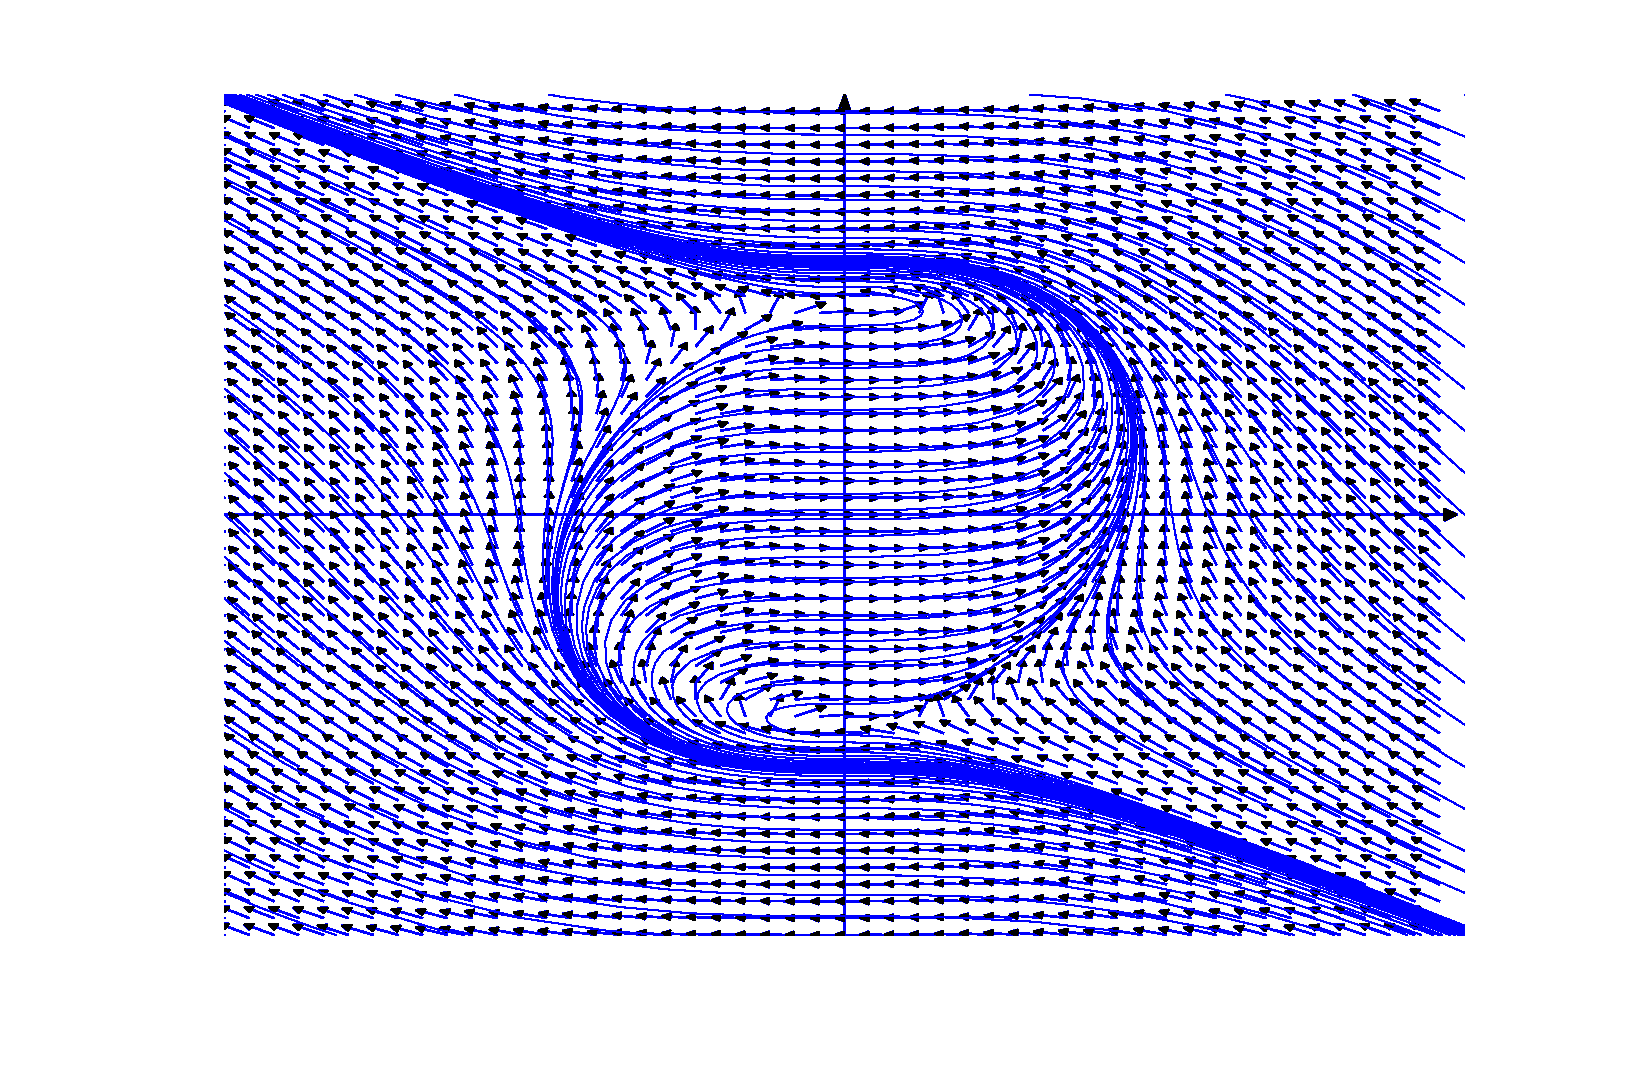
\includegraphics[bb=-78 148 689 643,width=5.67in,height=3.66in,keepaspectratio]{cover}
\end{figure}

%\vspace*{.2in}


\bf\huge
\href{http://ramanujan.math.trinity.edu/wtrench/index.shtml}
{William F. Trench}
\\\large
Andrew G. Cowles Distinguished Professor Emeritus\\
Department of Mathematics\\
Trinity University \\
San Antonio, Texas, USA\\
\href{mailto:{wtrench@trinity.edu}}
{wtrench@trinity.edu}
\large


\enlargethispage{2in}

\begin{quote}
This book has been judged to meet the evaluation criteria set by the
Editorial  Board
of the American Institute of Mathematics in connection with the Institute's
\href{http://www.aimath.org/textbooks/}
{Open
Textbook Initiative}.
It may be copied, modified, redistributed, translated,  and
built upon  subject to the  Creative Commons
\href{http://creativecommons.org/licenses/by-nc-sa/3.0/deed.en_G}
{Attribution-NonCommercial-ShareAlike 3.0 Unported
License}.
\end{quote}

\end{center}


\newpage
\vspace*{2in}
\thispagestyle{empty}
\vspace{1in}
\medskip

\noindent
{This book was  published previously by Brooks/Cole Thomson Learning}

\medskip

\noindent
 Reproduction  is
permitted
for any valid  noncommercial educational, mathematical, or scientific
purpose.
However,
charges for
profit beyond reasonable printing costs
are  prohibited.

\bigskip


\newpage
\setcounter{page}{1}
\pagenumbering{roman}
\thispagestyle{empty}
\noindent
\vspace*{3in}
\centerline{\bf\Huge TO BEVERLY}


\thispagestyle{empty}
\setcounter{page}{1}
\pagenumbering{roman}
\pdfbookmark[0]{Table of Contents}{contents}
\markboth
{\hskip1em Contents\hfill}
{\hfill Contents\hskip1em}
\vspace*{3.9pc}
\centerline{\bf \Huge Contents}
\vspace*{4.8pc}
\bf
  Chapter~1 \space Introduction\hskip1em
\hfill1

\vspace*{15pt}

1.2 \space First Order Equations\hfill1


\vspace*{15pt}

  Chapter~2 \space First Order Equations\hskip1em
\hfill5

\vspace*{15pt}

2.1 \space Linear First Order Equations\hfill5

2.2 \space Separable Equations \hfill8

2.3 \space Existence and Uniqueness of Solutions of Nonlinear Equations\hfill  11

2.4 \space Transformation of Nonlinear Equations into Separable Equations\hfill  13

2.5 \space Exact Equations\hfill    17

2.6 \space  Integrating Factors \hfill 21


\vspace*{15pt}

  Chapter~3 \space Numerical Methods\hskip1em
\hfill  25

\vspace*{15pt}

3.1 \space Euler's Method\hfill            25

3.2 \space The Improved Euler Method and Related Methods\hfill29

3.3 \space The Runge-Kutta Method\hfill  34

\vspace*{15pt}

  Chapter~4 \space Applications of First Order Equations\hskip1em
\hfill39

\vspace*{15pt}

 4.1 \space Growth and Decay \hfill 39

 4.2 \space Cooling and Mixing\hfill  40

 4.3 \space Elementary Mechanics\hfill  43

4.4 \space Autonomous Second Order Equations\hfill 45

4.5 \space Applications to Curves\hfill  46



  Chapter~5 \space Linear Second Order Equations\hskip1em
\hfill51

\vspace*{15pt}

5.1 \space Homogeneous Linear Equations\hfill 51

5.2 \space Constant Coefficient Homogeneous Equations\hfill 55

5.3 \space Nonhomgeneous Linear Equations\hfill  58

5.4 \space The Method of Undetermined Coefficients I\hfill 60


5.5 \space The Method of Undetermined Coefficients II\hfill 64


5.6 \space Reduction of Order\hfill   75

5.7 \space Variation of Parameters\hfill 79

\vspace*{15pt}

Chapter~6 \space   Applcations of Linear Second Order  Equations
\hfill85

\vspace*{15pt}

6.1 \space Spring Problems I\hfill 85


6.2 \space Spring Problems II\hfill   87

6.3 \space  The RLC Circuit\hfill  89

6.4 \space Motion Under a Central Force\hfill  90


\vspace*{15pt}


  Chapter~7 \space Series Solutions of Linear Second Order Equations\hskip1em
\hfill  108

\vspace*{15pt}

7.1 \space Review of Power Series\hfill 91

7.2  \space Series Solutions Near an Ordinary Point I\space \hfill  93


7.3  \space Series Solutions Near an Ordinary Point II\space \hfill  96


7.4 \space Regular Singular Points; Euler Equations\hfill    102

7.5 \space The Method of Frobenius I\space \hfill     103


7.6 \space The Method of Frobenius II\space \hfill108


7.7 \space The Method of Frobenius III \hfill   118


\vspace*{15pt}

Chapter~8 \space Laplace Transforms\hskip1em
\hfill       125

\vspace*{15pt}

8.1 \space Introduction to the Laplace Transform\hfill 125

8.2 \space The Inverse Laplace Transform\hfill   127

8.3 \space Solution of Initial Value Problems\hfill 134

8.4 \space The Unit Step Function\hfill               140

8.5 \space Constant Coefficient Equations with Piecewise Continuous
Forcing\\ \hspace*{.24in}Functions\hfill         143

8.6 \space Convolution\hfill152

8.7 \space Constant Cofficient Equations with Impulses\hfill55





\vspace*{15pt}

  Chapter~9 \space Linear Higher Order Equations\hskip1em
\hfill      159

\vspace*{15pt}

9.1 \space Introduction to Linear Higher Order Equations\hfill 159

9.2 \space Higher Order Constant Coefficient Homogeneous Equations\hfill
171

9.3 \space Undetermined Coefficients for Higher Order Equations\hfill
175

9.4 \space Variation of Parameters for Higher Order Equations\hfill  181

\vspace*{15pt}

  Chapter~10 \space  Linear Systems of Differential Equations\hskip1em
\hfill 221

\vspace*{15pt}

10.1 \space Introduction to Systems of Differential Equations\hfill 191

10.2 \space Linear Systems of Differential Equations\hfill 192

10.3 \space  Basic Theory of Homogeneous Linear Systems\hfill  193


10.4 \space Constant Coefficient Homogeneous Systems I\hfill 194


10.5 \space Constant Coefficient Homogeneous Systems II\hfill   201



10.6 \space Constant Coefficient Homogeneous Systems II\hfill     245



10.7 \space  Variation of Parameters for Nonhomogeneous Linear Systems\hfill
218

\vspace*{15pt}

  Chapter
\hfill 221

\vspace*{15pt}

11.1 \space Eigenvalue Problems for ${\mathbf y''+\lambda y=0}$\hfill 221

11.2 \space Fourier Expansions I\hfill  223


11.3 \space Fourier Expansions II\hfill 229


\vspace*{15pt}


  Chapter~12 \space Fourier  Solutions of Partial Differential
Equations\hskip1em
\hfill     239

\vspace*{15pt}

12.1 \space The Heat Equation\hfill     239

12.2 \space The Wave Equation\hfill    247

12.3 \space Laplace's Equation in Rectangular Coordinates\hfill   260

12.4 \space Laplace's Equation in Polar Coordinates\hfill   270


\vspace*{15pt}

Chapter~13\space Boundary Value Problems for Second Order Ordinary
Differential Equations  \hfill 273

13.1 Two-Point Boundary Value Problems  \hfill  273


13.2 Sturm-Liouville Problems  \hfill 279

\rm
\newpage
\setcounter{page}{1}
\pagenumbering{arabic}
\thispagestyle{empty}


\setcounter{chapter}{1}
\pagenumbering{arabic}
\setcounter{page}{1}
\thispagestyle{empty}
\pdfbookmark[0]{Chapter 1}{chapter:1}
\chaptertitle{Introduction}

\newsection{2}{Basic Concepts}{Basic Concepts}
\subpdfbookmark{Section 1.2} {section:1.2}

\newcommand{\thissection}{\sectiontitle{\,BASIC CONCEPTS}}
\thissection
      \vspace*{-17.5pt}


\exer{1.2.2}
\part{a} If $y=ce^{2x}$, then $y'=2ce^{2x}=2y$.

\part{b}  If $y=\dst {x^2\over3}+{c\over x}$, then
$y'=\dst{2x\over3}-{c\over x^2}$, so $xy'+y=\dst{2x^2\over3}-{c\over x
}+{x^2\over3}+{c\over x}=x^2$.

\part{c} If
$$
y=\dst{1\over2}+ce^{-x^2}, \mbox{\quad then \quad}
y'=-2xce^{-x^2}
$$
and
$$
y'+2xy=-2xce^{-x^2}+2x\dst\left({1\over2}+ce^{-x^2}\right)
=-2xce^{-x^2}+x+2cxe^{-x^2}=x.
$$

\part{d}
If
$$
y=\dst{1+ce^{-x^2/2}\over1-ce^{-x^2/2}}
$$
then
\begin{eqnarray*}
y'&=&{(1-ce^{-x^2/2})(-cxe^{-x^2/2})-(1+ce^{-x^2/2})cxe^{-x^2/2}\over
(1-cxe^{-x^2/2})^2}\\[2\jot]
&=&{-2cxe^{-x^2/2}\over(1-ce^{-x^2/2})^2}
\end{eqnarray*}
and
\begin{eqnarray*}
y^2-1&=&\left(1+ce^{-x^2/2}\over1-ce^{-x^2/2}\right)^2-1\\[2\jot]
&=&{(1+ce^{-x^2/2})^2-(1-ce^{-x^2/2})^2\over(1-ce^{-x^2/2})^2}\\[2\jot]
&=&{4ce^{-x^2/2}\over(1-ce^{-x^2/2})^2},
\end{eqnarray*}

\medskip
\centerline{1}


so
$$
2y'+x(y^2-1)={-4cx+4cx\over(1-ce^{-x^2/2})^2}=0.
$$


\part{e}
If $y=\dst\tan\left( {x^3\over3}+c\right)$, then
$y'=x^2\dst\sec^2\left({x^3\over3}+c\right)=
x^2\left(1+\tan^2\dst\left({x^3\over3+c}\right)\right)=
x^2(1+y^2)$.

\part{f}
If
\vspace*{-5ex}
\begin{eqnarray*}
y&=&(c_1+c_2x)e^x+\sin x+x^2,\mbox{\quad then}\\
y'&=&(c_1+2c_2x)e^x+\cos x+2x,\\
y'&=&(c_1+3c_2x)e^x-\sin x+2,\\
\arraytext{and}
y''-2y'+y&=&c_1e^x(1-2+1)+c_2xe^x(3-4+1)\\
&&-\sin x-2\cos x+\sin x+2-4x+x^2\\
&=&-2 \cos x+x^2-4x+2.
\end{eqnarray*}

\part{g} If $y=c_1e^x+c_2x+\dst{2\over x}$, then
$y'=c_1e^x+c_2-\dst{2\over x^2}$ and $y''=c_1e^x+\dst{4\over x^3}$, so
$(1-x)y''+xy'- y=c_1(1-x+x-1)+c_2(x-x)+\dst {4(1-x)\over x^3}-{2\over
x}-{2\over x}= {4(1-x-x^2)\over x^3}$

\part{h}
If $y=\dst{c_1\sin x+c_2 \cos x\over x^{1/2}}+4x+8$
then
 $y'=\dst{c_1\cos x-c_2 \sin x\over x^{1/2}}
-{c_1\sin x+c_2 \cos x\over 2x^{3/2}}+4$ and
$y''=-\dst{c_1\sin x+c_2 \cos x\over x^{1/2}}
-{c_1\sin x-c_2 \cos x\over x^{3/2}}+{3\over4}
{c_1\sin x+c_2 \cos x\over x^{5/2}}$, so
$\dst x^2y''+xy'+\left(x^2-{1\over4}\right)y=
c_1\left(-x^{-3/2}\sin x-x^{1/2}\cos x+
{3\over4}x^{-1/2}\sin x +x^{1/2}\cos x-\right.$
\mbox{}\\
$\dst\left.
{1\over2}x^{-1/2}\sin x+x^{3/2}\sin
x-{1\over4}x^{-1/2}
\sin x\right)+
\dst c_2\left(-x^{-3/2}\cos x+x^{1/2}\sin x
+{3\over4}x^{-1/2}\cos x \right.$
\mbox{}\\
$\dst\left.-x^{1/2}\sin x-{1\over2}x^{-1/2}\cos x+
 x^{3/2}\cos
x-{1\over4}x^{-1/2}\cos x\right)+4x+\left(x^2-{1\over4}\right)
(4x+8)=
4x^3+8x^2+3x-2$.


\exer{1.2.4}
\part{a} If $y'=-xe^x$, then
$y=-xe^x+\int e^x\,dx+c=(1-x)e^x+c$,
and $y(0)=1\Rightarrow 1=1+c$, so $c=0$ and $y=(1-x)e^x$.

\part{b}
If
$y'=x\sin x^2$, then
$y=-\dst{1\over2}\cos x^2+c$;
$\dst y\left({\sqrt{\pi\over2}}\right)=1 \Rightarrow 1=0+c$,
so $c=1$ and $y=1-\dst{1\over2}\cos x^2$.

\part{c} Write $y'=\tan x=\dst{\sin x\over\cos x}=-\dst{1\over\cos
x}{d\over dx}(\cos x)$. Integrating this yields $y=-\ln|\cos x|+c$;
 $y(\pi/4)=3\Rightarrow 3=-\ln\left(\cos(\pi/4)\right)+c$, or
$3=\ln\sqrt2+c$, so $c=3-\ln\sqrt2$, so
$y=-\ln(|\cos x|)+3-\ln\sqrt2=3-\ln(\sqrt2|\cos x|)$.

\part{d} If $y''=x^4$, then $y'=\dst{x^5\over5}+c_1$; $y'(2)=-1
\Rightarrow\dst{32\over5}+c_1=-1\Rightarrow c_1=-\dst{37\over15}$,
so $y'=\dst{x^5\over5}-{37\over15}$. Therefore, $y=\dst{x^6\over30}
-{37\over15}(x-2)+c_2$; $y(2)=-1\Rightarrow\dst{64\over30}+c_2=-1
\Rightarrow c_2=-\dst{47\over15}$, so
$y=-\dst{47\over15}-{37\over5}(x-2)+{x^6\over30}$.

\enlargethispage{1in}
\part{e} (A) $\int xe^{2x}\,dx=\dst{xe^{2x}\over2}-{1\over2}
\int e^{2x}\,dx={xe^{2x}\over2}-{e^{2x}\over4}$. Therefore,
$y'=\dst{xe^{2x}\over2}-{e^{2x}\over4}+c_1$; $y'(0)=1\Rightarrow
-\dst{1\over4}+c_1={5\over4}\Rightarrow c_1=\dst{5\over4}$,
so $y'=\dst{xe^{2x}\over2}-{e^{2x}\over4}+{5\over4}$;
Using (A) again,
$y=\dst{xe^{2x}\over4}-{e^{2x}\over8}-{e^{2x}\over8}+{5\over4}x+c_2
={xe^{2x}\over4}-{e^{2x}\over4}+{5\over4}x+c_2$; $y(0)=7
\Rightarrow-\dst{1\over4}+c_2=7\Rightarrow c_2=\dst{29\over4}$, so
$y=\dst{xe^{2x}\over4}-{e^{2x}\over4}+{5\over4}x+{29\over4}$.

\part{f} (A) $\int x\sin x\,dx=-x\cos x+\int \cos x\,dx=-x\cos x+\sin
x$ and (B) $\int x\cos x\,dx=x\sin x-\int\sin x\,dx=x\sin x+\cos x$.
If $y''=-x\sin x$, then (A) implies that $y'=x\cos x-\sin x+c_1$;
$y'(0)=-3\Rightarrow c=-3$, so $y'=x\cos x-\sin x-3$. Now (B) implies
that $y=x\sin x+\cos x+\cos x-3x+c_2=x\sin x+2\cos x-3x+c_2$;
$y(0)=1\Rightarrow 2+c_2=1\Rightarrow c_2=-1$, so $y=x \sin x+2 \cos
x-3x-1$.


\part{g} If $y'''=x^2e^x$, then $y''=\int x^2e^x\,dx=x^2e^x-2\int
xe^x\,dx=x^2e^x-2xe^x+2e^x+c_1$; $y''(0)=3\Rightarrow
2+c_1=3\Rightarrow c_1=1$, so (A) $y''=(x^2-2x+2)e^x+1$. Since $\int
(x^2-2x+2)e^x\,dx=(x^2-2x+2)e^x-\int (2x-2)e^x\,dx
=(x^2-2x+2)e^x-(2x-2)e^x+2e^x=(x^2-4x+6)e^x$, (A) implies that
$y'=(x^2-4x+6)e^x+x+c_2$; $y'(0)=-2\Rightarrow 6+c_2=-2\Rightarrow
c_2=-8$, so (B) $y'=(x^2-4x+6)e^x+x-8$; Since $\int
(x^2-4x+6)e^x\,dx=(x^2-4x+6)e^x-\int (2x-4)e^x\,dx
=(x^2-4x+6)e^x-(2x-4)e^x+2e^x=(x^2-6x+12)e^x$, (B) implies that
$y=(x^2-6x+12)e^x+\dst{x^2\over2}-8x+c_3$; $y(0)=1\Rightarrow
12+c_3=1\Rightarrow c_3=-11$, so
$y=(x^2-6x+12)e^x+\dst{x^2\over2}-8x-11$.

\part{h} If $y'''=2+\sin2x$, then $y''=\dst2x-{\cos 2x\over 2}+c_1$;
$y''(0)=3\Rightarrow -\dst{1\over 2}+c_1=3\Rightarrow c_1=\dst{7\over
2}$, so $y''=\dst2x-{\cos 2x\over 2}+{7\over 2}$. Then
$y'=x^2-\dst{\sin 2x\over 4}+{7\over 2}x+c_2$; $y'(0)=-6\Rightarrow
c_2=-6$, so $y'=x^2-\dst{\sin 2x\over 4}+{7\over 2}x-6$. Then
$y=\dst{x^3\over 3}+{\cos 2x\over 8}+{7\over 4}x^2-6x+c_3$;
$y(0)=1\Rightarrow \dst{1\over 8}+c_3=1\Rightarrow c_3=\dst{7\over
8}$, so $\dst y={x^3\over3}+{\cos 2x\over8}+
{7\over4}x^2-6x+{7\over8}$.

\part{i} If $y'''=2x+1$, then $y''=x^2+x+c_1$; $y''(2)=7\Rightarrow
6+c_1=7\Rightarrow c_1=1$; so $y''=x^2+x+1$. Then $y'=\dst{x^3\over
3}+{x^2\over 2}+(x-2)+c_2$; $y'(2)=-4\Rightarrow \dst{14\over
3}+c_2=-4\Rightarrow c_2=-\dst{26\over 3}$, so $y'=\dst{x^3\over
3}+{x^2\over 2}+(x-2)-{26\over 3}$. Then $y=\dst{x^4\over
12}+{x^3\over 6}+{1\over 2}(x-2)^2-{26\over 3}(x-2)+c_3$;
$y(2)=1\Rightarrow \dst{8\over 3}+c_3=1\Rightarrow c_3=-\dst{5\over
3}$, so $\dst y={x^4\over 12}+{x^3\over6}+{1\over2} (x-2)^2-{26\over3}
(x-2)-{5\over3}$.


\exer{1.2.6}
\part{a} If $y=x^2(1+\ln x)$, then $y(e)=e^2(1+\ln e)=2e^2$;
$y'=2x(1+\ln x)+x=3x+2x\ln x$, so $y'(e)=3e+2e\ln e=5e$; (A)
$y''=3+2+2\ln x=5+2\ln x$. Now, $3xy'-4y=3x(3x+2x\ln x)-4x^2(1+\ln
x)=5x^2+2x^2\ln x=x^2y''$, from (A).

\part{b} If $y=\dst{x^2\over3}+x-1$, then $y(1)=\dst{1\over
3}+1-1={1\over 3}$; $y'=\dst{2\over 3}x+1$, so $y'(1)=\dst{2\over
3}+1={5\over 3}$; (A) $y''=\dst{2\over 3}$. Now
$x^2-xy'+y+1=x^2-\dst x\left({2\over 3}x+1\right)+{x^2\over
3}+x-1+1={2\over 3}x^2=x^2y''$, from (A).

\part{c} If $y=(1+x^2)^{-1/2}$, then $y(0)=(1+0^2)^{-1/2}=1$;
$y'=-x(1+x^2)^{-3/2}$, so $y'(0)=0$; (A) $y''=(2x^2-1)(1+x^2)^{-5/2}$.
Now,
$(x^2-1)y-x(x^2+1)y'=(x^2-1)(1+x^2)^{-1/2}-x(x^2+1)(-x)(1+x^2)^{-3/2}
=(2x^2-1)(1+x^2)^{-1/2}=y''(1+x^2)^2$ from (A), so
$y''=\dst{(x^2-1)y-x(x^2+1)y'\over (x^2+1)^2}$.

\part{d} If $y=\dst{x^2\over 1-x}$, then $y(1/2)=\dst{1/4\over
1-1/2}={1\over 2}$; $y'=-\dst{x(x-2)\over(1-x)^2}$, so
$y'(1/2)=\dst{(-1/2)(-3/2)\over(1-1/2)^2}=3$; (A) $y''=\dst{2\over
(1-x)^3}$. Now, (B) $x+y=x+\dst{x^2\over1-x}={x\over1-x}$ and (C)
$xy'-y=\dst-{x^2(x-2)\over(1-x)^2}-{x^2\over1-x}={x^2\over(1-x)^2}$.
From (B) and (C), $(x+y)(xy'-y)=\dst{x^3\over(1-x)^3}={x^3\over2}y''$,
so $y''=\dst{2(x+y)(xy'-y)\over x^3}$.



\exer{1.2.8}
\part{a}
$y=(x-c)^a$ is defined and  $x-c=y^{1/a}$ on $(c,\infty)$;
moreover, $y'=a(x-c)^{a-1}=a\left(y^{1/a}\right)^{a-1}=ay^{(a-1)/a}$.

\part{b}  if $a>1$ or $a<0$, then $y\equiv0$  is a solution of
(B) on $(-\infty,\infty)$.


\exer{1.2.10}
\part{a} Since $y'=c$ we must show that the right side of
(B)  reduces to $c$ for all values of $x$
in some interval. If $y=c^2+cx+2c+1$,
\begin{eqnarray*}
x^2+4x+4y&=&x^2+4x+4c^2+4cx+8c+4\\
&=&x^2+4(1+c)x+4(c^2+2c+1)\\
&=&x^2+4(1+c)+2(c+1)^2=(x+2c+2)^2.
\end{eqnarray*}

Therefore, $\sqrt{x^2+4x+4y}=x+2c+2$ and the right side of
(B) reduces to $c$ if
$x>-2c-2$.


\part{b}
If $y_1=-\dst{x(x+4)\over4}$, then $y_1'=-\dst{x+2\over2}$
and $x^2+4x+4y=0$ for all $x$. Therefore, $y_1$ satisfies
(A) on $(-\infty,\infty)$.



\newpage

\thispagestyle{empty}
\setcounter{chapter}{2}
\pdfbookmark[0]{Chapter 2}{chapter:2}
\chaptertitle{First Order Equations}

\newsection{1}{First Order Equations}{Linear First Order Equations}
\subpdfbookmark{Section 2.1} {section:2.1}

\setcounter{section}{1}
\renewcommand{\thissection}
{\sectiontitle{\,LINEAR FIRST ORDER EQUATIONS}}
\thissection

\vspace{-20pt}





\exer{2.1.2}
$\dst{y'\over y}=-3x^2$;\quad $|\ln|y|=-x^3+k$;\quad $y=ce^{-x^3}$.
$y=ce^{-(\ln x)^2/2}$.

\exer{2.1.4}
$\dst{y'\over y}=-\dst{3\over x}$;\quad $\ln|y|=-3\ln|x|+k=-\ln|x|^3+k$;\quad
$y=\dst{c\over x^3}$.

\exer{2.1.6}
$\dst{y'\over y}=-\dst{1+x\over x}=-\dst{1\over x}-1$;\quad
$|\ln|y|=-\ln|x|-x+k$;\quad
$y=\dst{ce^{-x}\over x}$;\quad
$y(1)=1\Rightarrow
 c=e$;\quad
$y=\dst{e^{-(x-1)}\over x}$.


\exer{2.1.8}
$\dst{y'\over y}=-\dst{1\over x}-\cot x$;
\quad $|\ln|y|=-\ln|x|-\ln|\sin x|+k=-\ln|x\sin x|+k$;\quad
$y=\dst{c\over x\sin x}$;\quad $y(\pi/2)=2\Rightarrow
c=\pi$;\quad $y=\dst{\pi\over x\sin x}$.


\exer{2.1.10}
$\dst{y'\over y}=-\dst{k\over x}$;\quad
$|\ln|y|=-k\ln|x|+k_1=\ln|x^{-k}|+k_1$;\quad
$y=c|x|^{-k}$;\quad
$y(1)=3\Rightarrow c=3$;\quad $y=3x^{-k}$.


\exer{2.1.12}
 $\dst{y_1'\over y_1}=-3$;\quad $\ln|y_1|=-3x$;\quad
$y_1=e^{-3x}$;\quad $y=ue^{-3x}$;\quad
$u'e^{-3x}=1$;\quad $u'=e^{3x}$;\quad $u=\dst{e^{3x}\over3}+c$;\quad
$y=\dst{1\over3}+ce^{-3x}$.



\exer{2.1.14}
$\dst{y_1'\over y_1}=-2x$;\quad
$\ln|y_1|=-x^2$;\quad
$y_1=e^{-x^2}$;\quad
$y=ue^{-x^2}$;\quad
$u'e^{-x^2}=xe^{-x^2}$;\quad
$u'=x$;\quad
$u=\dst{x^2\over2}+c$;\quad
$y=e^{-x^2}\dst\left({x^2\over2}+c\right)$.



\exer{2.1.16}
$\dst{y_1'\over y_1}=-{1\over x}$;\quad
$\ln|y_1|=-\ln|x|$;\quad $y_1=\dst{1\over x}$;\quad $y=\dst{u\over
x}$;\quad
$\dst{u'\over x}=\dst{7\over x^2}+3$;\quad $u'=\dst{7\over
x}+3x$;\quad
$u=7\ln|x|+\dst{3x^2\over2}+c$;\quad $y=\dst{7\ln|x|\over
x}+\dst{3x\over2}+\dst{c\over x}$.

\medskip
\smallskip
\centerline{5}


\exer{2.1.18}
$\dst{y_1'\over y_1}=-{1\over x}-2x$; \quad
$\ln|y_1|=-\ln|x|-x^2$;\quad $y_1=\dst{e^{-x^2}\over x}$;\quad
$y=\dst{ue^{-x^2}\over x}$;\quad
$\dst{u'e^{-x^2}\over x}=x^2e^{-x^2}$;\quad
 $u'=x^3$;\quad
$u=\dst{x^4\over4}+c$;\quad
$y=e^{-x^2}\dst{\left({x^3\over4}+{c\over x}\right)}$.

\exer{2.1.20}
 $\dst{y_1'\over y_1}=-\tan x$;\quad
$\ln|y_1|=\ln|\cos x|$;\quad
$y_1=\cos x$;\quad $y=u\cos x$;\quad $u'\cos x=\cos x$;\quad
$u'=1$;\quad $u=x+c$;\quad $y=(x+c)\cos x$.


\exer{2.1.22}
$\dst{y_1'\over y_1}=\dst{4x-3\over(x-2)(x-1)}=\dst{5\over
x-2}-\dst{1\over x-1}$;\quad
$\ln|y_1|=5\ln|x-2|-\ln|x-1|=\dst{\ln\left|(x-2)^5\over
x-1\right|}$;\quad
$y_1=\dst{(x-2)^5\over x-1}$;\quad
 $y=\dst{u(x-2)^5\over x-1}$;\quad
$\dst{u'(x-2)^5\over x-1}=\dst{(x-2)^2\over x-1}$;\quad
$u'=\dst{1\over (x-2)^3}$;\quad
$u=-\dst{1\over 2}\dst{1\over(x-2)^2} +c$;\quad $y=-\dst{1\over
2}{(x-2)^3\over (x-1)}+c\dst{(x-2)^5\over (x-1)}$.


\exer{2.1.24}
$\dst{y_1'\over y_1}=-\dst{3\over x}$;\quad
$\ln|y_1|=-3\ln|x|=\ln|x|^{-3}$;\quad
$y_1=\dst{1\over x^3}$;\quad
$y=\dst{u\over x^3}$;\quad
$\dst{u'\over x^3}=\dst{e^x\over x^2}$;\quad
$u'=xe^x$;\quad
$u=xe^x-e^x+c$;\quad
$y=\dst{e^x\over x^2}-\dst{e^x\over x^3}+\dst{c\over x^3}$.



\exer{2.1.26}
$\dst{y_1'\over y_1}=-\dst{4x\over1+x^2}$;\quad
$\ln|y_1|=-2\ln(1+x^2)=\ln(1+x^2)^{-2}$;\quad
$y_1=\dst{1\over(1+x^2)^2}$;\quad
$y=\dst{u\over(1+x^2)^2}$;\quad
$\dst{u'\over(1+x^2)^2}={2\over(1+x^2)^2}$;\quad
$u'=2$;\quad
$u=2x+c$;\quad
$y=\dst{2x+c\over(1+x^2)^2}$;\quad
$y(0)=1\Rightarrow c=1$;\quad
$y=\dst{2x+1\over(1+x^2)^2}$.



\exer{2.1.28}
$\dst{y_1'\over y_1}=-\cot x$;\quad
$\ln|y_1|=-\ln|\sin x|$;\quad
$y_1=\dst{1\over\sin x}$;\quad
$y=\dst{u\over\sin x}$;\quad
$\dst{u'\over\sin x}=\cos x$;\quad
$u'=\sin x\cos x$;\quad
$u=\dst{\sin^2x\over2}+c$;\quad
$y=\dst{\sin x\over2}+c\csc x$;\quad
$y(\pi/2)=1\Rightarrow c={1\over2}$;\quad
$y=\dst{1\over2}(\sin x+\csc x)$.

\exer{2.1.30}
$\dst{y_1'\over y_1}=-\dst{3\over x-1}$;\quad
$\ln|y_1|=-3\ln|x-1|
=\ln|x-1|^{-3}$;\quad
$y_1=\dst{1\over(x-1)^3}$;\quad
$y=\dst{u\over(x-1)^3}$;\quad
$\dst{u'\over(x-1)^3}=
\dst{1\over(x-1)^4}+\dst{\sin
x\over(x-1)^3}$;\quad
$u'=\dst{1\over x-1}+\sin x$;\quad
$u=\ln|x-1|-\cos x+c$;\quad
$y=\dst{\ln|x-1|-\cos x+c\over(x-1)^3}$;\quad
$y(0)=1\Rightarrow c=0$;\quad
$y=\dst{\ln|x-1|-\cos x\over(x-1)^3}$.


\exer{2.1.32}
$\dst{y_1'\over y_1}=-\dst{2\over x}$;\quad
$\ln|y_1|=2\ln|x|=\ln(x^2)$;\quad
$y_1=x^2$;\quad
$y=ux^2$;\quad
$u'x^2=-x$;\quad
$u'=-\dst{1\over x}$;\quad
$u=-\ln|x|+c$;\quad
$y=x^2(c-\ln|x|)$;\quad
$y(1)=1\Rightarrow c=1$;\quad
$y=x^2(1-\ln x)$.


\exer{2.1.34}
$\dst{y_1'\over y_1}=-\dst{3\over x-1}$;\quad
$\ln|y_1|=-3\ln|x-1|=\ln|x-1|^{-3}$;\quad
$y_1=\dst{1\over(x-1)^3}$;\quad
$y=\dst{u\over(x-1)^3}$;\quad
$\dst{u'\over(x-1)^3}=\dst{1+(x-1)\sec^2x\over(x-1)^4}$;\quad
$u'=\dst{1\over x-1}+\sec^2x$;\quad
$u=\ln|x-1|+\tan x+c$;\quad
$y=\dst{\ln|x-1|+\tan x+c\over(x-1)^3}$;\quad
$y(0)=-1\Rightarrow c=1$;\quad
$y=\dst{\ln|x-1|+\tan
x+1\over(x-1)^3}$.



\exer{2.1.36}
$\dst{y_1'\over y_1}=\dst{2x\over x^2-1}$;\quad
$\ln|y_1|=\ln|x^2-1|$;\quad
$y_1=x^2-1$;\quad
$y=u(x^2-1)$;\quad
$u'(x^2-1)=x$;\quad
$u'=\dst{x\over x^2-1}$;\quad
$u=\dst{1\over2}\ln|x^2-1|+c$;\quad
$y=(x^2-1)\left(\dst{1\over2}\ln|x^2-1|+c\right)$;\quad
$y(0)=4\Rightarrow c=-4$;\quad
$y=(x^2-1)\left(\dst{1\over2}\ln|x^2-1|-4\right)$.


\exer{2.1.38}
$\dst{y_1'\over y_1}=-2x$;\quad
$\ln|y_1|=-x^2$;\quad
$y_1=e^{-x^2}$;\quad
$y=ue^{-x^2}$;\quad
$u'e^{-x^2}=x^2$;\quad
$u'=x^2e^{x^2}$;\quad
$u=c+\dst{\int_0^xt^2e^{t^2}\,dt}$;\quad
$y=e^{-x^2}\left(c+\dst{\int_0^xt^2e^{t^2}\,dt}\right)$;\quad
$y(0)=3\Rightarrow c=3$;\quad
$y=e^{-x^2}\left(3+\dst{\int_0^xt^2e^{t^2}\,dt}\right)$.


\exer{2.1.40}
$\dst{y_1'\over y_1}=-1$;\quad
$\ln|y_1|=-x$;\quad
$y_1=e^{-x}$;\quad
$y=ue^{-x}$;\quad
$u'e^{-x}=\dst{e^{-x}\tan x\over x}$;\quad
$u'=\dst{\tan x\over x}$;\quad
$u=c+\dst{\int_1^x\dst{\tan t\over t}\,dt}$;\quad
$y=e^{-x}\left(c+\dst{\int_1^x\dst{\tan t\over t}\,dt}\right)$;\quad
$y(1)=0\Rightarrow c=0$;\quad
$y=e^{-x}\dst{\int_1^x\dst{\tan t\over t}\,dt}$.


\exer{2.1.42}
$\dst{y_1'\over y_1}=-1-{1\over x}$;\quad
$\ln|y_1|=-x-\ln|x|$;\quad
$y_1=\dst{e^{-x}\over x}$;\quad
$y=\dst{ue^{-x}\over x}$;\quad
$\dst{u'e^{-x}\over x}=\dst{e^{x^2}\over x}$;\quad
$u'=e^xe^{x^2}$;\quad
$u=c+\dst{\int_1^xe^te^{t^2}\,dt}$;\quad
$y=\dst{{e^{-x}\over x}\left(c+\int_1^xe^te^{t^2}\,dt\right)}$;\quad
$y(1)=2\Rightarrow c=2e$;\quad
$y=\dst{{1\over
x}\left(2e^{-(x-1)}+e^{-x}\int_1^xe^te^{t^2}\,dt\right)}$.


\exer{2.1.44}
{\bf (b)} Eqn. (A) is equivalent to
$$
y'-{2\over x}=-{1\over x}
\eqno{\rm (B)}
$$
on $(-\infty,0)$ and $(0,\infty)$. Here
$\dst{y_1'\over y_1}=\dst{2\over x}$;\quad $\ln|y_1|=2\ln|x|$;\quad
$y_1=x^2$;\quad
$y=ux^2$;\quad $u'x^2=-\dst{1\over x}$;\quad $u'=-\dst{1\over
x^3}$;\quad
$u=\dst{1\over2x^2}+c$, so $y=\dst{1\over2}+cx^2$ is the general
solution of (A) on $(-\infty,0)$ and $(0,\infty)$.

{\bf (c)}
From the proof of \part{b}, any solution of (A) must be of the form
$$
y=\left\{\begin{array}{ll}\dst{{1\over2}+c_1x^2}, &x
\ge 0,\\[2\jot]
\dst{{1\over2}+c_2x^2}, &x < 0,\end{array}\right.
\eqno{\rm (C)}
$$
for $x\ne0$, and any function of the form (C)
satisfies (A) for $x\ne0$. To complete the proof we
must show that any function of the form (C) is
differentiable and satisfies (A) at $x=0$. By
definition,
$$
y'(0)=\lim_{x\to0}{y(x)-y(0)\over x-0}=\lim_{x\to0}{y(x)-1/2\over
x}
$$
if the limit exists. But
$$
{y(x)-1/2\over x}=\left\{\begin{array}{cl} c_1x,&x>0\\
c_2x,&x<0,\end{array}\right.
$$
so $y'(0)=0$. Since $0y'(0)-2y(0)=0\cdot0-2(1/2)=-1$, any function of
the form (C) satisfies (A) at
$x=0$.

{\bf (d)} From \part{b} any solution $y$ of (A) on
$(-\infty,\infty)$ is of the form (C), so
$y(0)=1/2$.

{\bf (e)} If $x_0>0$, then every function of the form
(C) with $c_1=\dst{y_0-1/2\over x_0^2}$ and $c_2$
arbitrary is a solution of the initial value problem on
$(-\infty,\infty)$. Since these functions are all identical on
$(0,\infty)$, this does not contradict Theorem~2.1.1, which
implies that (B) (so
(A)) has exactly one solution on $(0,\infty)$ such
that $y(x_0)=y_0$. A similar argument applies if $x_0<0$.


\exer{2.1.46}
{\bf (a)} Let $y=c_1y_1+c_2y_2$. Then
\begin{eqnarray*}
y'+p(x)y&=&(c_1y_1+c_2y_2)'+p(x)(c_1y_1+c_2y_2)\\[2\jot]
&=&c_1y_1'+c_2y_2'+c_1p(x)y_1+c_2p(x)y_2\\[2\jot]
&=&c_1(y_1'+p(x)y_1)+c_2(y_2+p(x)y_2)=c_1f_1(x)+c_2f_2(x).
\end{eqnarray*}

{\bf (b)}  Let $f_1=f_2=f$ and $c_1=-c_2=1$.

{\bf (c)}  Let $f_1=f$, $f_2=0$, and $c_1=c_2=1$.



\exer{2.1.48}
{\bf (a)}
If $z=\tan y$, then $z'=(\sec^2y)y'$, so $z'-3z=-1$;\;
$z_1=e^{3x}$;\;
$z=ue^{3x}$;\;
$u'e^{3x}=-1$;\;
$u'=-e^{-3x}$;\;
$u=\dst{e^{-3x}\over3}+c$;\;
$z=\dst{1\over3}+ce^{3x}=\tan y$;\;
$y=\tan^{-1}\dst{\left({1\over3}+ce^{3x}\right)}$.



{\bf (b)}
If $z=e^{y^2}$, then $z'=2yy'e^{y^2}$, so $z'+\dst{2\over
x}z=\dst{1\over x^2}$;\;
$z_1=\dst{1\over x^2}$;\;
$z=\dst{u\over x^2}$;\;
$\dst{u'\over x^2}=\dst{1\over x^2}$;\;
$u'=1$;\;
$u=x+c$;\;
$z=\dst{1\over x}+\dst{c\over x^2}=e^{y^2}$;\;
$y=\pm\dst{\left[\ln\left(\dst{1\over x}+\dst{c\over
x^2}\right)\right]^{1/2}}$.


{\bf (c)}
Rewrite the equation as $\dst{y'\over y}+\dst{2\over x}\ln y=4x$.
If $z=\ln y$, then $z'=\dst{y'\over y}$, so $z'+\dst{2\over x}z=4x$;
\
$z_1=\dst{1\over x^2}$;\;
$z=\dst{u\over x^2}$;\;
$\dst{u'\over x^2}=4x$;\;
$u'=4x^3$;\;
$u=x^4+c$;\;
$z=x^2+\dst{c\over x^2}=\ln y$;\;
$y=\exp\dst\left(x^2+{c\over x^2}\right)$.


{\bf (d)}
If $z=-\dst{1\over 1+y}$, then $z'=\dst{y'\over(1+y)^2}$, so
$z'+\dst{1\over x}z=-\dst{3\over x^2}$;\;
$z_1=\dst{1\over x}$;\;
$z=\dst{u\over x}$;\;
$\dst{u'\over x}=-\dst{3\over x^2}$;\;
$u'=-\dst{3\over x}$;\;
$u=-3\ln|x|-c$;\;
$z=-\dst{3\ln|x|+c\over x}=-\dst{1\over1+y}$;\;
$y=-1+\dst{x\over3\ln|x|+c}$.



\newsection{2}{First Order Equations}
{Separable Equations}
\currentpdfbookmark{Section 2.2}{section:2.2}
\renewcommand{\thissection}{\sectiontitle{\, SEPARABLE  EQUATIONS}}
\thissection
\vspace*{-15pt}






\exer{2.2.2}
By inspection, $y\equiv k\pi$ ($k=$integer) is a constant solution.
Separate variables to find others: $\dst{\left(\cos y\over\sin
y\right)}y'=-\sin x$;\ $\ln (|\sin y|)=\cos x+c$.



\exer{2.2.4}
 $y\equiv0$ is a  constant solution.
Separate variables to find others: $\dst{\left(\ln y\over
y\right)y'}=-x^2$;\ $\dst{(\ln y)^2\over2}=-{x^3\over3}+c$.


\exer{2.2.6}
 $y\equiv1$ and $y\equiv-1$ are constant solutions.
For others, separate variables:
$(y^2-1)^{-3/2}yy'=\dst{1\over x^2}$;\;
$-(y^2-1)^{-1/2}=-\dst{1\over x}-c=-\dst{\left(1+cx\over x\right)}$;\;
$(y^2-1)^{1/2}=\dst\left(x\over1+cx\right)$;\;
$(y^2-1)=\dst{\left(x\over1+cx\right)^2}$;\;
$y^2=1+\dst{\left(x\over1+cx\right)^2}$;\;
$y=\pm\dst{\left(1+\left(x\over1+cx\right)^2\right)^{1/2}}$.


\exer{2.2.8}
By inspection, $y\equiv0$ is a constant solution. Separate variables
to find others: $\dst{y'\over y}=-\dst{x\over1+x^2}$;\;
$\ln|y|=-\dst{1\over2}\ln(1+x^2)+k$;\;
 $y=\dst{c\over\sqrt{1+x^2}}$,
which includes the constant solution $y\equiv0$.


\exer{2.2.10}
$(y-1)^2y'=2x+3$;\ $\dst{(y-1)^3\over3}=x^2+3x+c$;\;
$(y-1)^3=3x^2+9x+c$;\;
$\dst{y=1+\big(3x^2+9x+c)^{1/3}}$.



\exer{2.2.12}
$\dst{y'\over y(y+1)}=-x$;\ $\dst{\left[{1\over y}-{1\over
y+1}\right]y'}=-x$;\ $\dst{\ln\left|y\over
y+1\right|}=-\dst{x^2\over2}+k$;\ $\dst{y\over
y+1}=ce^{-x^2/2}$;\ $y(2)=1\Rightarrow c=\dst{e^2\over2}$;\;
$y=(y+1)ce^{-x^2/2}$;\ $y(1-ce^{-x^2/2})=ce^{-x^2/2}$;\;
$y=\dst{ce^{-x^2/2}\over1-ce^{-x^2}/2}$;\ setting
$c=\dst{e^2\over2}$ yields
 $\dst{y={e^{-(x^2-4)/2}
\over2-e^{-(x^2-4)/2}}}$.


\exer{2.2.14}
$\dst{y'\over(y+1)(y-1)(y-2)}=-\dst{1\over x+1}$;\;
$\dst{\left[{1\over6}{1\over y+1}-{1\over2}{1\over
y-1}+{1\over3}{1\over y-2}\right]}y'=-{1\over x+1}$;\;
$\dst{\left[{1\over y+1}-{3\over y-1}+{2\over
y-2}\right]y'}=-\dst{6\over x+1}$;\;
$\ln|y+1|-3\ln|y-1|+2\ln|y-2|=-6\ln|x+1|+k$;\;
$\dst{(y+1)(y-2)^2\over(y-1)^3}=\dst{c\over(x+1)^6}$;\;
$y(1)=0\Rightarrow c=-256$;\;
$\dst{(y+1)(y-2)^2\over(y-1)^3}=-\dst{256\over(x+1)^6}$.


\exer{2.2.16}
$\dst{y'\over y(1+y^2)}=2x$;\ $\dst{\left[{1\over y}-{y\over
y^2+1}\right]y'}=2x$;\ $\dst{\ln\left(|y|\over
\sqrt{y^2+1}\right)}=x^2+k$;\ $\dst{y\over
\sqrt{y^2+1}}=ce^{x^2}$;\ $y(0)=1\Rightarrow c=\dst{1\over\sqrt2}$;\;
$\dst{y\over\sqrt{y^2+1}}=\dst{e^{x^2}\over\sqrt2}$;\;
$2y^2=(y^2+1)e^{x^2}$;\ $y^2(2-e^{x^2})=e^{2x^2}$;
$y=\dst{1\over\sqrt{2e^{-2x^2}-1}}$.


\exer{2.2.18}
$\dst{y'\over(y-1)(y-2)}=-2x$;\ $\dst{\left[{1\over
y-2}-{1\over y-1}\right]}y'=-2x$;\ $\dst{\ln\left|y-2\over
y-1\right|}=-x^2+k$;\ $\dst{y-2\over y-1}=ce^{-x^2}$;\;
$y(0)=3\Rightarrow c=\dst{1\over2}$;\ $\dst{y-2\over
y-1}=\dst{e^{-x^2}\over2}$;\ $y-2=\dst{e^{-x^2}\over2}(y-1)$;\;
$\dst{y\left(1-{e^{-x^2}\over2}\right)}=2-\dst{e^{-x^2}\over2}$;\;
$y=\dst{4-e^{-x^2}\over2-e^{-x^2}}$. \
The interval of validity is $(-\infty,\infty)$.



\exer{2.2.20}
$\dst{y'\over y(y-2)}=-1$;\ $\dst{{1\over2}\left[{1\over
y-2}-{1\over y}\right]y'}=-1$;\;
 $\dst{\left[{1\over
y-2}-{1\over y}\right]y'}=-2$;\ $\dst{\ln\left|y-2\over
y\right|}=-2x+k$;\ $\dst{y-2\over y}=ce^{-2x}$;\;
$y(0)=1\Rightarrow c=-1$;\ $\dst{y-2\over y}=-e^{-2x}$;\;
$y-2=-ye^{-2x}$;\ $y(1+e^{-2x})=2$;\;
   $y=\dst{2\over
1+e^{-2x}}$. The interval of validity is $(-\infty,\infty)$.


\exer{2.2.22}
$y\equiv2$ is a constant solution of the differential equation, and
it satisfies the initial condition. Therefore, $y\equiv2$ is a
solution of the initial value problem. The interval of validity is
$(-\infty,\infty)$.



\exer{2.2.24}
$\dst{y'\over1+y^2}=\dst{1\over1+x^2}$;\ $\tan^{-1}y=
\tan^{-1}x+k$;\ $y=\tan(\tan^{-1}x+k)$. Now use
the identity $\tan(A+B)=\dst{\tan A+\tan B\over1-\tan A\tan B}$ with
$A=\tan^{-1}x$ and $B=\tan^{-1}c$ to rewrite $y$ as
$y=\dst{x+c\over1-cx}$, where $c=\tan k$.

\exer{2.2.26}
$(\sin y)y'=\cos x$;\ $-\cos
y=\sin x+c$;\  $y(\pi)=\dst{\pi\over2}\Rightarrow
c=0$, so (A)  $\cos y=-\sin
x$. To obtain $y$ explicity we  note that $-\sin x=\cos(x+\pi/2)$, so
(A) can be rewritten as  $\cos y=\cos(x+\pi/2)$. This equation
holds if an only if one of the following conditions holds for some
integer $k$:
$$
\mbox{(B)}\ y=x+{\pi\over2}+2k\pi;\\mbox{(C)}\
y=-x-{\pi\over2}+2k\pi.
$$
Among these choices the only way to satisfy the initial condition
is to let $k=1$ in (C), so $y=-x+\dst{3\pi\over2}.$



\exer{2.2.28}
Rewrite the equation as $P'=-a\alpha P(P-1/\alpha)$.
By inspection, $P\equiv0$ and $P\equiv1/\alpha$ are constant
solutions.
Separate variables to find others: $\dst{P'\over
P(P-1/\alpha)}=-a\alpha$;\;
 $\dst{\left[{1\over P-1/\alpha}-{1\over P}\right]P'}=-a
$;\ $\dst{\ln\left|P-1/\alpha\over P\right|}=-at+k$;\;
(A) $\dst{P-1/\alpha\over
P}=ce^{-\alpha t}$; $P(1-ce^{-\alpha t})=1/\alpha$;\;
(B) $P=\dst{1\over\alpha(1-ce^{-\alpha t})}$. From (A),
 $P(0)=P_0\Rightarrow c=\dst{P_0-1/\alpha\over P_0}$.
Substituting this into (B) yields
$P=\dst{P_0\over\alpha
P_0+(1-\alpha P_0)e^{-at}}$. From this
$\lim_{t\to\infty}P(t)=1/\alpha$.


\exer{2.2.30}
If $q=rS$ the equation for $I$ reduces to $I'=-rI^2$, so
$\dst{I'\over I^2}=-r$; $-\dst{1\over I}=-rt-\dst{1\over I_0}$;
so $I=\dst{I_0\over1+rI_0t}$ and $\lim_{t\to\infty}I(t)=0$. If $q\ne
rS$, then rewrite the equation for $I$ as $I'=-rI(I-\alpha)$ with
$\alpha=S-\dst{q\over r}$. Separating variables yields
$\dst{I'\over I(I-\alpha)}=-r$;\;
 $\dst{\left[{1\over I-\alpha}-{1\over I}\right]I'}=-r\alpha
$;\ $\dst{\ln\left|I-\alpha\over I\right|}=-r\alpha t+k$;\;
(A) $\dst{I-\alpha\over
I}=ce^{-r\alpha t}$; $I(1-ce^{-r\alpha t})=\alpha$;\;
(B) $I=\dst{\alpha\over 1-ce^{-r\alpha t}}$. From (A),
 $I(0)=I_0\Rightarrow c=\dst{I_0-\alpha\over I_0}$.
Substituting this into (B) yields
$I=\dst{\alpha I_0\over I_0+(\alpha-I_0)e^{-r\alpha t}}$.
If $q<rS$, then $\alpha>0$ and
$\lim_{t\to\infty}I(t)=\alpha=S-\dst{q\over r}$.
If $q>rS$, then $\alpha<0$ and $\lim_{t\to\infty}I(t)=0$.


\exer{2.2.34}
The given equation is separable if $f=ap$, where $a$ is a constant.
In this case the equation is
$$
y'+p(x)y=ap(x).
\eqno{\rm (A)}
$$
Let $P$ be an antiderivative  of $p$; that is, $P'=p$.

{\sc Solution by Separation of Variables.} $y'=-p(x)(y-a)$;\;
$\dst{y'\over y-a}=-p(x)$;\ $\ln|y-a|=-P(x)+k$;\;
$y-a=ce^{-P(x)}$;\ $y=a+ce^{-P(x)}$.

{\sc Solution by Variation of Parameters.} $y_1=e^{-P(x)}$
is a solution of the complementary equation, so solutions of
(A) are of the form $y=ue^{-P(x)}$ where
$u'e^{-P(x)}=ap(x)$. Hence, $u'=ap(x)e^{P(x)}$;\;
$u=ae^{P(x)}+c$;\ $y=a+ce^{-P(x)}$.


\exer{2.2.36} Rewrite the given equation as
(A) $y'-\dst{2\over x}y=\dst{x^5\over y+x^2}$.
 $y_1=x^2$ is a solution of $y'-\dst{2\over x}y=0$.
Look for solutions of (A)  of the form $y=ux^2$.
Then $u'x^2=\dst{x^5\over(u+1)x^2}=\dst{x^3\over u+1}$;\;
$u'=\dst{x\over u+1}$;\;
$(u+1)u'=x$;\;
$\dst{(1+u)^2\over2}=\dst{x^2\over2}+\dst{c\over2}$;\;
$u=-1\pm\sqrt{x^2+c}$;\ $y=x^2\left(-1\pm\sqrt{x^2+c}\right)$.


\exer{2.2.38}
$y_1=e^{2x}$ is a solution of $y'-2y=0$.
Look for solutions of the nonlinear equation of the form $y=ue^{2x}$.
Then $u'e^{2x}=\dst{xe^{2x}\over1-u}$;\ $u'=\dst{x\over1-u}$;\;
$(1-u)u'=x$;\;
$-\dst{(1-u)^2\over2}=\dst{1\over2}(x^2-c)$;\;
$u=1\pm\sqrt{c-x^2}$;\;
$y=e^{2x}\left(1\pm\sqrt{c-x^2}\right)$.



\newsection{3}{First Order Equations}
{Existence and Uniqueness of Solutions of Nonlinear Equations}
\currentpdfbookmark{Section 2.3}{section:2.3}
\renewcommand{\thissection}{\sectiontitle{\,
EXISTENCE AND UNIQUENESS OF SOLUTIONS OF NONLINEAR EQUATIONS }}
\thissection
\vspace*{-15pt}




\exer{2.3.2}
$f(x,y)=\dst{e^x+y\over x^2+y^2}$ and $f_y(x,y)=\dst{1\over
x^2+y^2}-\dst{2y(e^x+y)\over(x^2+y^2)^2}$ are both continuous at all
$(x,y)\ne(0,0)$. Hence,  Theorem~2.3.1 implies that if
$(x_0,y_0)\ne(0,0)$, then  the initial
value problem has a a unique solution on some open interval containing
$x_0$.  Theorem~2.3.1 does not apply
if $(x_0,y_0)=(0,0)$.

\exer{2.3.4}
$f(x,y)=\dst{x^2+y^2\over\ln xy}$ and $f_y(x,y)=\dst{2y\over\ln
xy}-\dst{x^2+y^2\over x(\ln xy)^2}$ are both continuous at all $(x,y)$
such that $xy>0$ and $xy\ne1$. Hence,  Theorem~2.3.1 implies
that if
$x_0y_0>0$ and $x_0y_0\ne1$, then the
initial value problem has unique solution on an open interval
containing $x_0$.   Theorem~2.3.1 does not apply
if $x_0y_0\le0$ or $x_0y_0=1$.


\exer{2.3.6}
$f(x,y)=2xy$ and $f_y(x,y)=2x$ are both continuous at all $(x,y)$.
Hence,  Theorem~2.3.1 implies that if $(x_0,y_0)$
is arbitrary, then the initial value problem
has a  unique solution on some open interval containing  $x_0$.


\exer{2.3.8}
$f(x,y)=\dst{2x+3y\over x-4y}$ and $f_y(x,y)=\dst{3\over
x-4y}+4\dst{2x+3y\over(x-4y)^2}$ are both continuous at all $(x,y)$
such that $x\ne4y$. Hence,  Theorem~2.3.1 implies that if
$x_0\ne4y_0$, then the
initial value problem has a  unique solution on some open interval
containing  $x_0$.
  Theorem~2.3.1 does not apply if $x_0=4y_0$.

\exer{2.3.10}
$f(x,y)=x(y^2-1)^{2/3}$ is continuous at all $(x,y)$, but
$f_y(x,y)=\dst{4\over3}xy(y^2-1)^{1/3}$ is continuous at $(x,y)$ if
and only if $y\ne\pm1$. Hence,  Theorem~2.3.1 implies that
if $y_0\ne\pm1$, then the
initial value problem has a  unique solution on some open interval
containing  $x_0$, while  if $y_0=\pm1$, then the initial value problem
 has at least one solution (possibly not unique on any
open interval containing  $x_0$).


\exer{2.3.12}
$f(x,y)=(x+y)^{1/2}$ and $f_y(x,y)=\dst{1\over2(x+y)^{1/2}}$ are both
continuous at all $(x,y)$ such that $x+y>0$ Hence,
 Theorem~2.3.1 implies that if $x_0+y_0>0$, then the initial
value problem has a
 unique solution on some open interval containing  $x_0$.
 Theorem~2.3.1 does not apply if $x_0+y_0\le0$.

\exer{2.3.14}
To apply  Theorem~2.3.1, rewrite the given initial value problem
as (A) $y'=f(x,y),\ y(x_0)=y_0$, where $f(x,y)=-p(x)y+q(x)$ and
$f_y(x,y)=-p(x)$. If $p$ and $f$ are continuous on some open interval
$(a,b)$ containing $x_0$, then $f$ and $f_y$ are continuous on some
open
rectangle containing $(x_0,y_0)$, so  Theorem~2.3.1 implies
that (A) has a unique solution  on {\it some\/} open
interval
containing $x_0$. The conclusion of Theorem~2.1.2 is more
specific:
the solution of (A) exists and is unique on $(a,b)$. For example, in
the extreme case where $(a,b)=(-\infty,\infty)$,  Theorem~2.3.1
still implies only existence and uniqueness on {\it some\/} open
interval containing $x_0$, while  Theorem~2.1.2 implies that the
solution exists and is unique on $(-\infty,\infty)$.


\exer{2.3.16}
First find solutions of (A) $y'=y^{2/5}$. Obviously $y\equiv0$ is a
solution. If $y\not\equiv0$, then we can separate variables on any
open interval where $y$ has no zeros: $y^{-2/5}y'=1$;\;
$\dst{5\over3}y^{3/5}=x+c$;\;
$y=\dst{\left({3\over5}(x+c)^{5/3}\right)}$. (Note that this solution
is also defined  at $x=-c$, even though  $y(-c)=0$. To satisfy the
initial condition, let $c=1$. Thus,
$y=\dst{\left({3\over5}(x+1)^{5/3}\right)}$ is a solution of the
initial value problem on $(-\infty,\infty)$; moreover,
since $f(x,y)=y^{2/5}$ and $f_y(x,y)=\dst{2\over5}y^{-3/5}$
are both continuous  at all $(x,y)$ such that $y\ne0$,
this is the only
solution on $(-5/3,\infty)$, by an argument similar to that given in
Example~2.3.7, the function
$$
y =
\dst{\left\{
\begin{array}{cl}
0, &  -\infty< x \le -{5\over 3} \\[3pt]
\left({3\over 5}x + 1\right)^{5/3}, & -{5\over3} < x < \infty
\end{array}\right.}
$$
(To see that $y$ satisfies $y'=y^{2/5}$  at $x=-\dst{5\over3}$
use an argument similar to that of
Discussion~2.3.15-2)
For every $\dst{a \ge {5\over 3}}$, the following function is also a
solution:
$$
y =
\left\{
\begin{array}{cl}
\left( {3\over 5} (x+a) \right)^{5/3}, & - \infty < x < -a, \\[3pt]
0, &  -a \le x \le -{5\over 3} \\[3pt]
\left({3\over 5}x + 1\right)^{5/3}, & -{5\over3} < x < \infty.
\end{array}\right.
$$


\exer{2.3.18}
Obviously, $y_1\equiv1$ is a solution.
From Discussion~2.3.18 (taking $c=0$
in the two families of solutions) yields
$y_2=1+|x|^3$ and $y_3=1-|x|^3$. Other solutions are
$y_4=1+x^3$, $y_5=1-x^3$,
$$
y_6=\dst{\left\{\begin{array}{ccl}1+x^3,&x\ge 0,\\
1,&x<0\end{array}\right.};\quad
y_7=\dst{\left\{\begin{array}{ccl}1-x^3,&x\ge 0,\\
1,&x<0\end{array}\right.};
$$
$$
y_8=\dst{\left\{\begin{array}{ccl}1,&x\ge 0,\\
1+x^3,&x<0\end{array}\right.};\quad
y_9=\dst{\left\{\begin{array}{ccl}1,&x\ge 0,\\
1-x^3,&x<0\end{array}\right.}
$$


It is straightforward to verify that all these functions satisfy
$y'=3x(y-1)^{1/3}$  for all $x\ne0$. Moreover,
 $y_i'(0)=\dst{\lim_{x\to0}{y_i(x)-1\over x}}=0$ for
$1\le i\le 9$, which implies that they also satisfy the equation at
$x=0$.



\exer{2.3.20}
Let $y$ be any solution of (A) $y'=3x(y-1)^{1/3},\ y(3)=-7$.
By continuity, there is some open interval $I$ containing  $x_0=3$
on which $y(x)<1$. From
Discussion~2.3.18,
 $y=1+(x^2+c)^{3/2}$ on $I$;\ $y(3)=-7\Rightarrow c=-5$;\;
(B) $y=1-(x^2-5)^{3/2}$.  It now follows that every solution of (A)
satisfies $y(x)<1$
and is given by (B) on $(\sqrt5,\infty)$; that is,
(B) is the unique solution of (A) on
$(\sqrt5,\infty)$.
 This solution can be extended uniquely to
$(0,\infty)$ as
$$
y=
\left\{
\begin{array}{cl}
1, & 0< x\le\sqrt5,\\
1-(x^2-5)^{3/2}, & \sqrt5<x<\infty
\end{array}\right.
$$
It can be extended to $(-\infty,\infty)$ in infinitely many ways.
Thus,
$$
\dst y= \left\{
\begin{array}{cl}
 1, &-\infty< x\le\sqrt5,\\
1-(x^2-5)^{3/2},& \sqrt5<x<\infty
\end{array} \right.$$
is a solution of the initial value problem on $(-\infty,\infty)$.
Moroever, if
$\alpha\ge0$, then
$$
y= \left\{
\begin{array}{cl}
 1+(x^2-\alpha^2)^{3/2},& -\infty<x<-\alpha, \\
1, & -\alpha\le x\le\sqrt5,\\
1-(x^2-5)^{3/2},& \sqrt5<x<\infty,
\end{array}\right. $$
and
$$
y= \left\{
\begin{array}{cl}
 1-(x^2-\alpha^2)^{3/2},& -\infty<x<-\alpha, \\
1, & -\alpha\le x\le\sqrt5,\\
1-(x^2-5)^{3/2},& \sqrt5<x<\infty,
\end{array} \right.
$$
are also solutions of the initial value problem  on
$(-\infty,\infty)$.



\vspace*{5pt}
\newsection{4}{First Order Equations}
{Transformation of Nonlinear Equations into Separable Equations}
\currentpdfbookmark{Section 2.4}{section:2.4}
\renewcommand{\thissection}{\sectiontitle{\,
TRANSFORMATION OF NONLINEAR EQUATIONS INTO SEPARABLE EQUATIONS }}
\thissection

\vspace*{-17.5pt}





\exer{2.4.2}
 Rewrite as $y'-\dst{2\over7x}y=-\dst{x\over7y^6}$. Then
$\dst{y_1'\over y_1}=\dst{2\over7x}$;\;
$\ln|y_1|=\dst{2\over7}\ln|x|=\ln|x|^{2/7}$;\;
$y_1=x^{2/7}$;\;
$y=ux^{2/7}$;\;
$u'x^{2/7}=-\dst{1\over7u^6x^{5/7}}$;\;
$u^6u'=-\dst{1\over7x}$;\;
$\dst{u^7\over7}=-\dst{1\over7}\ln|x|+\dst{c\over7}$;\;
$u=(c-\ln|x|)^{1/7}$;\;
$y=x^{2/7}(c-\ln|x|)^{1/7}$.


\exer{2.4.4}
 Rewrite as $y'+\dst{2x\over1+x^2}y=\dst{1\over(1+x^2)^2y}$.
Then
$\dst{y_1'\over y_1}=-\dst{2x\over1+x^2}$;\;
$\ln|y_1|=-\ln(1+x^2)$;\;
$y_1=\dst{1\over1+x^2}$;\;
$y=\dst{u\over1+x^2}$;\;
$\dst{u'\over1+x^2}=\dst{1\over u(1+x^2)}$;\;
$u'u=1$;\;
$\dst{u^2\over2}=x+\dst{c\over2}$;\;
$u=\pm\sqrt{2x+c}$;\;
$y=\pm\dst{{\sqrt{2x+c}\over1+x^2}}$.


\exer{2.4.6}
$\dst{y_1'\over y_1}=\dst{{1\over3}\left({1\over x}+1\right)}$;\;
$\ln|y_1|=\dst{1\over3}(\ln|x|+x)$;\;
$y_1=x^{1/3}e^{x/3}$;\;
$y=ux^{1/3}e^{x/3}$;\;
$u'x^{1/3}e^{x/3}=x^{4/3}e^{4x/3}u^4$;\;
$\dst{u'\over u^4}=xe^x$;\;
$-\dst{1\over3u^3}=(x-1)e^x-\dst{c\over3}$;\;
$u=\dst{1\over[3(1-x)e^x+c]^{1/3}}$;\;
$y=\dst{\left[x\over3(1-x)+ce^{-x}\right]^{1/3}}$.


\exer{2.4.8}
$\dst{y_1'\over y_1}=x$;\;
$\ln|y_1|=\dst{x^2\over2}$;\;
$y_1=e^{x^2/2}$;\;
$y=ue^{x^2/2}$;\;
$u'e^{x^2/2}=xu^{3/2}e^{3x^2/4}$;\;
$\dst{u'\over u^{3/2}}=xe^{x^2/4}$;\;
(A) $-\dst{2\over u^{1/2}}=2e^{x^2/4}+2c$;\;
$u^{1/2}=-\dst{1\over c+e^{x^2/4}}$;\;
$u^=\dst{1\over(c+e^{x^2/4})^2}$;\;
$y=\dst{1\over(1+ce^{-x^2/4})^2}$. Because of (A) we must choose $c$
so that $y(1)=4$ and $1+ce^{-1/4}<0$. This implies that
$c=-3e^{1/4}$;\;
$y=\dst{\left[1-{3\over2}e^{-(x^2-1)/4}\right]^{-2}}$.


\exer{2.4.10}
$\dst{y_1'\over y_1}=2$;\;
$\ln|y_1|=2x$;\;
$y_1=e^{2x}$;\;
$y=ue^{2x}$;\;
$u'e^{2x}=2u^{1/2}e^x$;\;
$u^{-1/2}u'=2e^{-x}$;\;
$2u^{1/2}=-2e^{-x}+2c$;\;
$u^{1/2}=c-e^{-x}>0$;\;
$y(0)=1\Rightarrow u(0)=1\Rightarrow
c=2$;\;
$u=(2-e^{-x})^2$;\;
$y=(2e^x-1)^2$.


\exer{2.4.12}
Rewrite as $y'+\dst{2\over x}y=\dst{y^3\over x^2}$. Then
$\dst{y_1'\over y_1}=-\dst{2\over x}$;\;
$\ln|y_1|=-2\ln|x|=\ln x^{-2}$;\;
$y_1=\dst{1\over x^2}$;\;
$y=\dst{u\over x^2}$;\;
$\dst{u'\over x^2}=\dst{u^3\over x^8}$;\;
$\dst{u'\over u^3}=\dst{1\over x^6}$;\;
$-\dst{1\over2u^2}=-\dst{1\over5x^5}+c$;\;
$y(1)=\dst{1\over\sqrt2}\Rightarrow u(1)=\dst{1\over\sqrt2}\Rightarrow
c=-\dst{4\over5}$;\;
$u=\dst{\left[5x^5\over2(1+4x^5)\right]^{1/2}}$;\;
$y=\dst{\left[5x\over2(1+4x^5)\right]^{1/2}}$.


\exer{2.4.14}
$P=ue^{at}$;\ $u'e^{at}=-a\alpha u^2e^{2at}$;\ $\dst{u'\over
u^2}=-a\alpha e^{at}$;\ $-\dst{1\over
u}=-a\int_0^t\alpha(\tau)e^{a\tau}\,d\tau-\dst{1\over P_0}$;\;
$P=\dst{P_0e^{at}\over1+aP_0\int_0^t\alpha(\tau)e^{a\tau}\,d\tau}$,
which can also be written as
$P=\dst{P_0\over
e^{-at}+aP_0e^{-at}\int_0^t\alpha(\tau)e^{a\tau}\,d\tau}$.
Therefore, $\lim_{t\to\infty}P(t)=
\dst{\left\{\begin{array}{rl}\infty&\mbox{ if }L=0,\\0&\mbox{ if
}L=\infty,\\ 1/aL&\mbox{ if } 0<L<\infty.\end{array}\right.}$

\exer{2.4.16}
$y=ux$;\ $u'x+u=u^2+2u$;\;
(A) $u'x=u(u+1)$. Since $u\equiv0$ and $u\equiv-1$ are constant
solutions of (A), $y\equiv0$ and $y=-x$ are
solutions of the given equation. The nonconstant solutions of (A)
satisfy
$=\dst{u'\over u(u+1)}={1\over x}$;\;
$\dst{\left[{1\over u}-{1\over u+1}\right]u'}=\dst{1\over x}$;\;
$\dst{\ln\left|u\over u+1\right|}=\ln|x|+k$;\;
$\dst{u\over u+1}=cx$;\ $u=(u+1)cx$;\ $u(1-cx)=cx$;\;
$u=\dst{cx\over1-cx}$;\;
$y=\dst{cx^2\over1-cx}$.

\exer{2.4.18}
$y=ux$;\ $u'x+u=u+\sec$;\;
$u'x=\sec u$;\;
$(\cos u)u'=\dst{1\over x}$;\;
$\sin u=\ln|x|+c$;\;
$u=\sin^{-1}(\ln|x|+c)$;\;
$y=x\sin^{-1}(\ln|x|+c)$.



\exer{2.4.20}
Rewrite the given equation as $y'=\dst{x^2+2y^2\over xy}$;\;
$y=ux$;\ $u'x+u=\dst{1\over u}+2u$;\;
$u'x=\dst{1+u^2\over u}$;\;
$\dst{uu'\over1+u^2}=\dst{1\over x}$;\;
$\dst{1\over2}\ln(1+u^2)=\ln|x|+k$;\;
$\dst{\ln\left(1+{y^2\over x^2}\right)}=\ln x^2+2k$;\;
$\dst{1+{y^2\over x^2}}=cx^2$;\;
$x^2+y^2=cx^4$;\ $y=\pm x\sqrt{cx^2-1}$.



\exer{2.4.22}
$y=ux$;\ $u'x+u=u+u^2$;\;
$u'x=u^2$;\;
$\dst{u'\over u^2}=\dst{1\over x}$;\;
$-\dst{1\over u}=\ln|x|+c$;\;
$y(-1)=2\Rightarrow u(-1)=-2\Rightarrow c=\dst{1\over2}$;\;
$u=-\dst{2\over2\ln|x|+1}$;\;
$y=-\dst{2x\over2\ln|x|+1}$.


\exer{2.4.24}
Rewrite the given equation as $y'=-\dst{x^2+y^2\over xy}$;\;
$y=ux$;\ $u'x+u=-\dst{1\over u}-u$;\;
$u'x=-\dst{1+2u^2\over u}$;\;
$-\dst{uu'\over1+2u^2}=\dst{1\over x}$;\;
$-\dst{1\over4}\ln(1+2u^2)=\ln|x|+k$;\;
$x^4(1+2u^2)=c$;\;
$y(1)=2\Rightarrow u(1)=2\Rightarrow c=9$;\;
$x^4(1+2u^2)=9$;\;
$u^2=\dst{9-x^4\over2x^4}$;\;
$u=\dst{1\over x^2}\dst{\left(9-x^4\over2\right)^{1/2}}$;\;
$y=\dst{1\over x}\dst{\left(9-x^4\over2\right)^{1/2}}$.

\exer{2.4.26}
Rewrite the given equation as $y'=2+\dst{y^2\over
x^2}+4\dst{y\over x}$;\;
$y=ux$;\ $u'x+u=2+u^2+4u$;\;
$u'x=u^2+3u+2=(u+1)(u+2)$;\;
$\dst{u'\over(u+1)(u+2)}=\dst{1\over x}$;\;
$\dst{\left[{1\over u+1}-{1\over u+2}\right]u'}=\dst{1\over x}$;\;
$\dst{\ln\left|u+1\over u+2\right|}=\ln|x|+k$;\;
$\dst{u+1\over u+2}=cx$;\;
$y(1)=1\Rightarrow u(1)=1\Rightarrow c=\dst{2\over3}$;\;
$\dst{u+1\over u+2}=\dst{2\over3}x$;\;
$u+1=\dst{2\over3}x(u+2)$;\;
$u\dst{\left(1-{2\over3}x\right)}=-1+\dst{4\over3}x$;\;
$u=-\dst{4x-3\over2x-3}$;\;
$y=-\dst{x(4x-3)\over2x-3}$.

\exer{2.4.28}
$y=ux$;\ $u'x+u=\dst{1+u\over1-u}$;\;
$u'x=\dst{1+u^2\over1-u}$;\;
$\dst{(1-u)u'\over1+u^2}=\dst{1\over x}$;\;
$\tan^{-1}u-\dst{1\over2}\ln(1+u^2)=\ln|x|+c$;\;
$\tan^{-1}\dst{y\over
x}-\dst{1\over2}\ln\dst{\left(1+{y^2\over x^2}\right)}=\ln|x|+c$;\;
$\tan^{-1}\dst{y\over
x}-\dst{1\over2}\ln(x^2+y^2)=c$.

\exer{2.4.30}
$y=ux$;
$u'x+u=\dst{u^3+2u^2+u+1\over(u+1)^2}=\dst{u(u+1)^2+1\over(u+1)^2}
=u+\dst{1\over(u+1)^2}$;
$u'x=\dst{1\over(u+1)^2}$;\;
$(u+1)^2u'=\dst{1\over x}$;\;
$\dst{(u+1)^3\over3}=\ln|x|+c$;\;
$(u+1)^3=3(\ln|x|+c)$;\;
$\dst\left({y\over x}+1\right)^3=3(\ln|x|+c)$;\;
$(y+x)^3=3x^3(\ln|x|+c)$.



\exer{2.4.32}
$y=ux$;\ $u'x+u=\dst{u\over u-2}$;\;
(A)  $u'x=\dst{u(u-3)\over2-u}$;\;
Since $u\equiv0$ and $u\equiv3$
are constant solutions of (A), $y\equiv0$ and
$y=3x$ are solutions of the given equation.
The nonconstant solutions of (A) satisfy
$\dst{(2-u)u'\over u(u-3)}=\dst{1\over x}$;\;
$\dst{\left[{1\over u-3}+{2\over
u}\right]u'}=-\dst{3\over x}$;\;
$\ln|u-3|+2\ln|u|=-3\ln|x|+k$;\;
$u^2(u-3)=\dst{c\over x^3}$;\;
$y^2(y-3x)=c$.


\exer{2.4.34}
$y=ux$;\;
$u'x+u=
\dst {1+u+3u^3 \over 1+3u^2}=u+{1 \over 1+3u^2}$;\;
$(1+3u^2)u'=\dst{1\over x}$;\;
$u+u^3=\ln |x|+c$;\;
$\dst{{y\over x}+{y^3\over x^3}}=\ln |x|+c$.


\exer{2.4.36}
Rewrite the given equation as $y'=\dst{x^2-xy+y^2\over xy}$;\;
$y=ux$;\ $u'x+u=\dst{1\over u}-1+u$;\;
$u'x=\dst{1-u\over u}$;\;
$\dst{uu'\over u-1}=-\dst{1\over x}$;\;
$\dst{\left[1+{1\over u-1}\right]u'}=-\dst{1\over x}$;\;
$u+\ln|u-1|=-\ln|x|+k$;\;
$e^u(u-1)=\dst{c\over x}$;\;
$e^{y/x}(y-x)=c$.



\exer{2.4.38}
$y=ux$;\;
$u'x+u=1+\dst{1\over u}+u$;\;
(A) $u'x=\dst{u+1\over u}$.
Since (A)  has the constant solution $u=-1$;
$y=-x$ is
a solution of the given equation. The nonconstant solutions of (A)
satisfy
$\dst{uu'\over u+1}=\dst{1\over x}$;\;
$\dst{\left[1-{1 \over u+1}\right]u'}={1\over x}$;\;
$u-\ln |u+1|=\ln |x|+c$;\;
$\dst{y\over x}-\dst{\ln\left|{y\over x}-1\right|}=\ln|x|+c$;\;
$y-x\ln|y-x|=cy$.

\exer{2.4.40}
If $x=X-X_0$ and $y=Y-Y_0$, then $\dst{dy\over dx}=\dst{dY\over
dx}=\dst{dY\over dX}\dst{dX\over dx}=\dst{dY\over dX}$, so $y=y(x)$
satisfies the given equation if and only if $Y=Y(X)$ satisfies
 $$
{dY\over dX}=\dst{a(X-X_0)+b(Y-Y_0)+\alpha\over
c(X-X_0)+d(Y-Y_0)+\beta},
$$
 which reduces to the nonlinear homogeneous equation
$$
{dY\over dX}=\dst{aX+bY\over cX+dY}
$$
 if and only if
$$
\begin{array}{rcl}
aX_0+bY_0&=&\alpha\\
cX_0+dY_0&=&\beta.
\end{array}
\eqno{\rm (B)}
$$
We will now show that
if $ad-bc\ne0$, then it is possible (for any choice of $\alpha$
and $\beta$) to solve (B).
Multiplying the first equation in (B) by $d$ and
 the second by  $b$ yields
\begin{eqnarray*}
daX_0+dbY_0&=&d\alpha  \\
bcX_0+bdY_0&=&b\beta.
\end{eqnarray*}
Subtracting the second of these equations from the first yields
 $(ad-bc)X_0=\alpha d-\beta b$.
Since $ad-bc\ne0$, this implies that $X_0=\dst{\alpha d-\beta b\over
ad-bc}$. Multiplying the first equation in (B) by
$c$ and the second by $a$ yields
\begin{eqnarray*}
caX_0+cbY_0&=&c\alpha  \\
acX_0+adY_0&=&a\beta.
\end{eqnarray*}
Subtracting the first of these equation from the second yields
 $(ad-bc)Y_0=\alpha c-\beta a$. Since $ad-bc\ne0$ this implies that
$Y_0=\dst{\alpha c-\beta a\over ad-bc}$.


\exer{2.4.42}
For the given equation, (B)
of Exercise~2.4.40 is
\begin{eqnarray*}
2X_0+Y_0&=&\phantom{-}1\\
X_0+2Y_0&=&-4.
\end{eqnarray*}
Solving this pair of equations yields   $X_0=2$ and $Y_0=-3$.
The transformed differential equation is
$$
{dY\over dX}=\dst{2X+Y\over X+2Y}.
\eqno{\rm (A)}
$$
Let $Y=uX$;\;
$u'X+U=\dst{2+u\over1+2u}$;\;
(B) $u'X=-\dst{2(u-1)(u+1)\over 2u+1}$. Since $u\equiv1$ and
$u\equiv-1$
satisfy (B), $Y=X$ and $Y=-X$ are solutions of (A).
 Since $X=x+2$ and $Y=y-3$, it follows that $y=x+5$
and $y=-x+1$ are solutions of the given equation. The nonconstant
solutions of (B) satisfy
$\dst{(2u+1)u'\over(u-1)(u+1)}=-\dst{2\over X}$;\;
$\dst{\left[{1\over u+1}+{3\over u-1}\right]u'}=-\dst{4\over
X}$;\;
$\ln|u+1|+3\ln|u-1|=-4\ln|X|+k$;\;
$\dst{(u+1)(u-1)^3}=\dst{c\over X^4}$;\;
$(Y+X)(Y-X)^3=c$;\;
Setting $X=x+2$ and $Y=y-3$ yields
$(y+x-1)(y-x-5)^3=c$.


\exer{2.4.44}
Rewrite the given equation as $y'=\dst{y^3+x\over3xy^2}$;\;
$y=ux^{1/3}$;\;
$u'x^{1/3}+\dst{1\over3x^{2/3}}u=\dst{u^3+1\over3u^2x^{2/3}}$;\;
$u'x^{1/3}=\dst{1\over3x^{2/3}u^2}$;\;
$u^2u'=\dst{1\over3x}$;\;
$\dst{u^3\over3}=\dst{1\over3}(\ln|x|+c)$;\;
$u=(\ln|x|+c)^{1/3}$;\;
$y=x^{1/3}(\ln|x|+c)^{1/3}$.


\exer{2.4.46}
Rewrite the given equation as $y'=\dst{2(y^2+x^2y-x^4)\over
x^3}$;\;
$y=ux^2$;\;
$u'x^2+2xu=2x(u^2+u-1)$;\;
(A) $u'x^2=2x(u^2-1)$.
Since $u\equiv1$ and $u\equiv-1$ are constant solutions of (A),
$y=x^2$ and $y=-x^2$ are solutions of the given equation. The
nonconstant solutions of (A) satisfy
$\dst{u'\over u^2-1}=\dst{2\over x}$;\;
$\dst{\left[{1\over u-1}-{1\over u+1}\right]u'}=\dst{4\over x}$;\;
$\dst{\ln\left|u-1\over u+1\right|}=4\ln|x|+k$;\;
$\dst{u-1\over u+1}=cx^4$;\;
$(u-1)=(u+1)cx^4$;\;
$u(1-cx^4)=1+cx^4$;\;
$u=\dst{1+cx^4\over1-cx^4}$;\;
$y=\dst{x^2(1+cx^4)\over1-cx^4}$.


\exer{2.4.48}
$y=u\tan x$;\;
$u'\tan x+u\sec^2x=(u^2+u+1)\sec^2x$;\;
$u'\tan x=(u^2+1)\sec^2x$;\;
$\dst{u'\over u^2+1}=\sec^2x\cot x=\cot x+\tan x$;\;
$\tan^{-1}u=\ln|\sin x|-\ln|\cos x|+c=\ln|\tan x|+c$;\;
$u=\tan(\ln|\tan x|+c)$;\;
$y=\tan x\ \tan(\ln|\tan x|+c)$.


\exer{2.4.50}
Rewrite the given equation as $y'=\dst{(y+\sqrt
x)^2\over2x(y+2\sqrt x)}$;\;
$y=ux^{1/2}$;\;
$u'x^{1/2}+\dst{1\over2\sqrt x}u=\dst{(u+1)^2\over2\sqrt x\
(u+2)}$;\;
$u'x^{1/2}=\dst{1\over2\sqrt x\ (u+2)}$;\;
$(u+2)u'=\dst{1\over2x}$;\;
$\dst{(u+2)^2\over2}=\dst{1\over2}(\ln|x|+c)$;\;
$(u+2)^2=\ln|x|+c$;\;
$u=-2\pm\sqrt{\ln|x|+c}$;\;
$y=x^{1/2}(-2\pm\sqrt{\ln|x|+c})$.


\exer{2.4.52}
$y_1=\dst{1\over x^2}$ is a solution of $y'+\dst{2\over x}y=0$.
Let $y=\dst{u\over x^2}$; then
$$
\dst{u'\over x^2}=\dst{3x^2(u^2/x^4)+6x(u/x^2)+2\over
x^2\left(2x(u/x^2)+3\right)}=
\dst{3(u/x)^2+6(u/x)+2\over x^2\left(2(u/x)+3\right)},
$$
so (A) $u'=\dst{3(u/x)^2+6(u/x)+2\over2(u/x)+3}$. Since (A)
is a homogeneous nonlinear equation, we now substitute $u=vx$
into (A). This yields
$v'x+v=\dst{3v^2+6v+2\over2v+3}$;\;
$v'x=\dst{(v+1)(v+2)\over2v+3}$;\;
$\dst{(2v+3)v'\over(v+1)(v+2)}=\dst{1\over x}$;\;
$\dst{\left[{1\over v+1}+{1\over v+2}\right]v'}=\dst{1\over x}$;\;
$\ln|(v+1)(v+2)|=\ln|x|+k$;\;
(B) $(v+1)(v+2)=cx$.
Since $y(2)=2\Rightarrow u(2)=8\Rightarrow v(2)=4$, (B) implies that
$c=15$.\ $(v+1)(v+2)=15x$;\;
$v^2+3v+2-15x=0$. From the quadratic formula,
$v=\dst{-3+\sqrt{1+60x}\over2}$;\;
$u=vx=\dst{x(-3+\sqrt{1+60x})\over2}$;\;
$y=\dst{u\over x^2}=\dst{-3+\sqrt{1+60x}\over2x}$.


\exer{2.4.54}
Differentiating  (A) $y_1(x)=\dst{y(ax)\over a}$   yields
(B) $y_1'(x)=\dst{1\over a}y'(ax)\cdot a=y'(ax)$. Since
$y'(x)=q(y(x)/x)$ on some interval $I$, (C) $y'(ax)=q(y(ax)/ax)$
on some interval $J$. Substituting (A) and (B) into (C)
yields $y_1'(x)=q(y_1(x)/x)$ on $J$.


\exer{2.4.56}
  If $y=z+1$, then
$z'+z=xz^2$;\;
$z=ue^{-x}$;\;
$u'e^{-x}=xu^2e^{-2x}$;\;
$\dst{u'\over u^2}=xe^{-x}$;\;
$-\dst{1\over u}=-e^{-x}(x+1)-c$;\;
$u=\dst{1\over e^{-x}(x+1)+c}$;\;
$z=\dst{1\over x+1+ce^x}$;\;
$y=1+\dst{1\over x+1+ce^x}$.


\exer{2.4.58}
If $y=z+1$, then
$z'+\dst{2\over x}z=z^2$;\;
$z_1=\dst{1\over x^2}$;\;
$z=\dst{u\over x^2}$;\;
$\dst{u'\over x^2}=\dst{u^2\over x^4}$;\;
$\dst{u'\over u^2}=\dst{1\over x^2}$;\;
$-\dst{1\over u}=-\dst{1\over x}+c=-\dst{1-cx\over x}$;\;
$u=-\dst{x\over 1-cx}$;\;
$z=-\dst{1\over x(1-cx)}$;\;
$y=1-\dst{1\over x(1-cx)}$.

\newsection{5}{First Order Equations}
{Exact Equations}
\currentpdfbookmark{Section 2.5}{section:2.5}
\renewcommand{\thissection}{\sectiontitle{\,
EXACT EQUATIONS}}
\thissection

\vspace*{-10pt}






\exer{2.5.2}
$M(x,y)=3y\cos x+4xe^x+2x^2e^x$;\;
$N(x,y)=3\sin x+3$;\;
$M_y(x,y)=3\cos x=N_x(x,y)$,
so the  equation is exact.
We must find $F$ such that
(A) $F_x(x,y)=3y\cos x+4xe^x+2x^2e^x$ and
(B) $F_y(x,y)=3\sin x+3$.
Integrating (B) with respect to $y$ yields
(C) $F(x,y)=3y\sin x+3y+\psi(x)$.
Differentiating (C) with respect to $x$  yields
(D) $F_x(x,y)=3y\cos x+\psi'(x)$.
Comparing (D) with (A)  shows that
(E) $\psi'(x)=4xe^x+2x^2e^x$.
Integration by parts yields
$\dst{\int}xe^x\,dx=xe^x-e^x$ and
$\dst{\int}x^2e^x\,dx=x^2e^x-2xe^x+2e^x$.
Substituting from the last two equations into (E) yields
$\psi(x)=2x^2e^x$.
Substituting this into (C) yields
$F(x,y)=3y\sin x+3y+2x^2e^x$.
Therefore, $3y\sin x+3y+2x^2e^x=c$.


\exer{2.5.4}
$M(x,y)=2x-2y^2$;\;
$N(x,y)=12y^2-4xy$;\;
$M_y(x,y)=-4y=N_x(x,y)$,
so the  equation is exact.
We must find $F$ such that
(A) $F_x(x,y)=2x-2y^2$ and
(B) $F_y(x,y)=12y^2-4xy$.
Integrating (A) with respect to $x$ yields
(C) $F(x,y)=x^2-2xy^2+\phi(y)$.
Differentiating (C) with respect to $y$  yields
(D) $F_y(x,y)=-4xy+\phi'(y)$.
Comparing (D) with (B)  shows that
$\phi'(y)=12y^2$, so we take
$\phi(y)=4y^3$.
Substituting this into (C) yields
$F(x,y)=x^2-2xy^2+4y^3$.
Therefore, $x^2-2xy^2+4y^3=c$.


\exer{2.5.6}
$M(x,y)=4x+7y$;\;
$N(x,y)=3x+4y$;\;
$M_y(x,y)=7\ne3=N_x(x,y)$,
so the  equation is not exact.

\exer{2.5.8}
$M(x,y)=2x+y$;\;
$N(x,y)=2y+2x$;\;
$M_y(x,y)=1\ne2=N_x(x,y)$,
so the  equation is not exact.


\exer{2.5.10}
$M(x,y)=2x^2+8xy+y^2$;\;
$N(x,y)=2x^2+\dst{xy^3\over3}$;\;
$M_y(x,y)=8x+2y\ne4x+\dst{y^3\over3}=N_x(x,y)$,
so the  equation is not exact.


\exer{2.5.12}
$M(x,y)=y\sin xy+xy^2\cos xy$;\;
$N(x,y)=x\sin xy+xy^2\cos xy$;\;
$M_y(x,y)=3xy\cos xy+(1-x^2y^2)\sin xy\ne(xy+y^2)\cos
xy+(1-xy^3)\sin xy=N_x(x,y)$, so the equation is not exact.


\exer{2.5.14}
$M(x,y)=e^x(x^2y^2+2xy^2)+6x$;\;
$N(x,y)=2x^2ye^x+2$;\;
$M_y(x,y)=2xye^x(x+2)=N_x(x,y)$,
so the  equation is  exact.
We must find $F$ such that
(A) $F_x(x,y)=e^x(x^2y^2+2xy^2)+6x$ and
(B) $F_y(x,y)=2x^2ye^x+2$.
Integrating (B) with respect to $y$ yields
(C) $F(x,y)=x^2y^2e^x+2y+\psi(x)$.
Differentiating (C) with respect to $x$  yields
(D) $F_x(x,y)=e^x(x^2y^2+2xy^2)+\psi'(x)$.
Comparing (D) with (A)  shows that
$\psi'(x)=6x$, so we take
$\psi(x)=3x^2$.
Substituting this into (C) yields
$F(x,y)=x^2y^2e^x+2y+3x^2$.
Therefore, $x^2y^2e^x+2y+3x^2=c$.


\exer{2.5.16}
$M(x,y)=e^{xy}(x^4y+4x^3)+3y$;\;
$N(x,y)=x^5e^{xy}+3x$;\;
$M_y(x,y)=x^4e^{xy}(xy+5)+3=N_x(x,y)$,
so the  equation is  exact.
We must find $F$ such that
(A) $F_x(x,y)=e^{xy}(x^4y+4x^3)+3y$ and
(B) $F_y(x,y)=x^5e^{xy}+3x$.
Integrating (B) with respect to $y$ yields
(C) $F(x,y)=x^4e^{xy}+3xy+\psi(x)$.
Differentiating (C) with respect to $x$  yields
(D) $F_x(x,y)=e^{xy}(x^4y+4x^3)+3y+\psi'(x)$.
Comparing (D) with (A)  shows that
$\psi'(x)=0$, so we take
$\psi(x)=0$.
Substituting this into (C) yields
$F(x,y)=x^4e^{xy}+3xy$.
Therefore,  $x^4e^{xy}+3xy=c$.


\exer{2.5.18}
$M(x,y)=4x^3y^2-6x^2y-2x-3$;\;
$N(x,y)=2x^4y-2x^3$;\;
$M_y(x,y)=8x^3y-6x^2=N_x(x,y)$,
so the  equation is exact.
We must find $F$ such that
(A) $F_x(x,y)=4x^3y^2-6x^2y-2x-3$ and
(B) $F_y(x,y)=2x^4y-2x^3$.
Integrating (A) with respect to $x$ yields
(C) $F(x,y)=x^4y^2-2x^3y-x^2-3x+\phi(y)$.
Differentiating (C) with respect to $y$  yields
(D) $F_y(x,y)=2x^4y-2x^3+\phi'(y)$.
Comparing (D) with (B)  shows that
$\phi'(y)=0$, so we take
$\phi(y)=0$.
Substituting this into (C) yields
$F(x,y)=x^4y^2-2x^3y-x^2-3x$.
Therefore, $x^4y^2-2x^3y-x^2-3x=c$.
Since $y(1)=3\Rightarrow c=-1$,
$x^4y^2-2x^3y-x^2-3x+1=0$ is an implicit solution of the initial
value problem. Solving this for $y$ by means of the quadratic formula
yields $y=\dst{x+\sqrt{2x^2+3x-1}\over x^2}$.


\exer{2.5.20}
$M(x,y)=(y^3-1)e^x$;\;
$N(x,y)=3y^2(e^x+1)$;\;
$M_y(x,y)=3y^2e^x=N_x(x,y)$,
so the  equation is exact.
We must find $F$ such that
(A) $F_x(x,y)=(y^3-1)e^x$ and
(B) $F_y(x,y)=3y^2(e^x+1)$.
Integrating (A) with respect to $x$ yields
(C) $F(x,y)=(y^3-1)e^x+\phi(y)$.
Differentiating (C) with respect to $y$  yields
(D) $F_y(x,y)=3y^2e^x+\phi'(y)$.
Comparing (D) with (B)  shows that
$\phi'(y)=3y^2$, so we take
$\phi(y)=y^3$.
Substituting this into (C) yields
$F(x,y)=(y^3-1)e^x+y^3$.
Therefore, $(y^3-1)e^x+y^3=c$.
Since $y(0)=0\Rightarrow c=-1$,
$(y^3-1)e^x+y^3=-1$ is an implicit solution of  the initial value
problem. Therefore, $y^3(e^x+1)=e^x-1$, so
$y=\dst{\left(e^x-1\over e^x+1\right)^{1/3}}$.


\exer{2.5.22}
$M(x,y)=(2x-1)(y-1)$;\;
$N(x,y)=(x+2)(x-3)$;\;
$M_y(x,y)=2x-1=N_x(x,y)$,
so the  equation is exact.
We must find $F$ such that
(A) $F_x(x,y)=(2x-1)(y-1)$ and
(B) $F_y(x,y)=(x+2)(x-3)$.
Integrating (A) with respect to $x$ yields
(C) $F(x,y)=(x^2-x)(y-1)+\phi(y)$.
Differentiating (C) with respect to $y$  yields
(D) $F_y(x,y)=x^2-x+\phi'(y)$.
Comparing (D) with (B)  shows that
$\phi'(y)=-6$, so we take
$\phi(y)=-6y$.
Substituting this into (C) yields
$F(x,y)=(x^2-x)(y-1)-6y$.
Therefore, $(x^2-x)(y-1)-6y=c$.
Since $y(1)=-1\Rightarrow c=6$,
$(x^2-x)(y-1)-6y=6$ is an implicit solution of  the initial value
problem. Therefore, $(x^2-x-6)y=x^2-x+6$, so
$y=\dst{x^2-x+6\over(x-3)(x+2)}$.


\exer{2.5.24}
$M(x,y)=e^x(x^4y^2+4x^3y^2+1)$;\;
$N(x,y)=2x^4ye^x+2y$;\;
$M_y(x,y)=2x^3ye^x(x+4)=N_x(x,y)$,
so the  equation is  exact.
We must find $F$ such that
(A) $F_x(x,y)=e^x(x^4y^2+4x^3y^2+1)$ and
(B) $F_y(x,y)=2x^4ye^x+2y$.
Integrating (B) with respect to $y$ yields
(C) $F(x,y)=x^4y^2e^x+y^2+\psi(x)$.
Differentiating (C) with respect to $x$  yields
(D) $F_x(x,y)=e^xy^2(x^4+4x^3)+\psi'(x)$.
Comparing (D) with (A)  shows that
$\psi'(x)=e^x$, so we take
$\psi(x)=e^x$.
Substituting this into (C) yields
$F(x,y)=(x^4y^2+1)e^x+y^2$.
Therefore, $(x^4y^2+1)e^x+y^2=c$.


\exer{2.5.28}
$M(x,y)=x^2+y^2$;\;
$N(x,y)=2xy$;\;
$M_y(x,y)=2y=N_x(x,y)$,
so the  equation is exact.
We must find $F$ such that
(A) $F_x(x,y)=x^2+y^2$ and
(B) $F_y(x,y)=2xy$.
Integrating (A) with respect to $x$ yields
(C) $F(x,y)=\dst{x^3\over3}+xy^2+\phi(y)$.
Differentiating (C) with respect to $y$  yields
(D) $F_y(x,y)=2xy+\phi'(y)$.
Comparing (D) with (B)  shows that
$\phi'(y)=0$, so we take
$\phi(y)=0$.
Substituting this into (C) yields
$F(x,y)=\dst{x^3\over3}+xy^2$.
Therefore, $\dst{x^3\over3}+xy^2=c$.


\exer{2.5.30}
{\bf (a)}
Exactness requires that
$N_x(x,y)=M_y(x,y)=\dst{\partial\over\partial
y}(x^3y^2+2xy+3y^2)=2x^3y+2x+6y$.
 Hence, $N(x,y)=\dst{x^4y\over4}+x^2+6xy+g(x)$,
where $g$ is  differentiable.

{\bf (b)}
Exactness requires that
$N_x(x,y)=M_y(x,y)=\dst{\partial\over\partial y}(\ln xy+2y\sin
x)=\dst{1\over y}+2\sin x$.
 Hence, $N(x,y)=\dst{x\over y}-2\cos x+g(x)$,
where $g$ is  differentiable.

{\bf (c)}
Exactness requires that
$N_x(x,y)=M_y(x,y)=\dst{\partial\over\partial y}(x\sin x+y\sin
y)=y\cos y+\sin y$.
 Hence, $N(x,y)=x(y\cos y+\sin y)+g(x)$,
where $g$ is  differentiable.

\exer{2.5.32}
 The assumptions imply that
$\dst{\partial M_1\over\partial y}=\dst{\partial N_1\over\partial x}$\
and\ $\dst{\partial M_2\over\partial y}=\dst{\partial N_2\over\partial
x}$. Therefore, $\dst{\partial \over\partial
y}(M_1+M_2)=\dst{\partial M_1\over\partial y}+\dst{\partial
M_2\over\partial y}=\dst{\partial N_1\over\partial x}+\dst{\partial
N_2\over\partial x}=\dst{\partial \over\partial x}(N_1+N_2)$,
which implies that $(M_1+M_2)\,dx+(N_1+N_2)\,dy=0$ is exact on $R$.


\exer{2.5.34}
Here $M(x,y)=Ax^2+Bxy+Cy^2$ and
$N(x,y)=Dx^2+Exy+Fy^2$. Since $M_y=Bx+2Cy$ and $N_x=2Dx+Ey$, the
equation is exact if and only if $B=2D$ and $E=2C$.


\exer{2.5.36}
Differentiating (A)
$F(x,y)=\dst{\int^y_{y_0}N(x_0,s)\,ds}+\dst{\int^x_{x_0}M(t,y)\,dt}$
with respect to $x$ yields $F_x(x,y)=M(x,y)$, since the first
integral
in (A) is independent of $x$ and $M(t,y)$ is a continuous function
of
$t$ for each fixed $y$. Differentiating  (A)  with respect to $y$
and using the assumption that $M_y=N_x$ yields
$F_y(x,y)=N(x_0,y)+\dst{\int^x_{x_0}{\partial M
\over\partial y}(t,y)\,dt}
=N(x_0,y)+\dst{\int^x_{x_0}{\partial N
\over\partial x} (t,y)\,dt}
=N(x_0,y)+N(x,y)-N(x_0,y)=N(x,y)$.


\exer{2.5.38}
$y_1=\dst{1\over x^2}$ is a solution of $y'+\dst{2\over x}y=0$.
Let $y=\dst{u\over x^2}$; then
$$
\dst{u'\over x^2}=-\dst{2x(u/x^2)\over
\left(x^2+2x^2(u/x^2)+1\right)}=
-\dst{2xu\over x^2(x^2+2u+1)},
$$
so  $u'=-\dst{2xu\over x^2+2u+1}$, which can be rewritten as (A)
$2xu\,dx+(x^2+2u+1)\,du=0$. Since $\dst{\dst{\partial \over\partial
u}}(2xu)=\dst{\dst{\partial \over\partial x}}(x^2+2u+1)=2x$, (A)
is exact. To solve (A)
we must find $F$ such that
(A) $F_x(x,u)=2xu$ and
(B) $F_u(x,u)=x^2+2u+1$.
Integrating (A) with respect to $x$ yields
(C) $F(x,u)=x^2u+\phi(u)$.
Differentiating (C) with respect to $u$  yields
(D) $F_u(x,u)=x^2+\phi'(u)$.
Comparing (D) with (B)  shows that
$\phi'(u)=2u+1$, so we take
$\phi(u)=u^2+u$.
Substituting this into (C) yields
$F(x,u)=x^2u+u^2+u=u(x^2+u+1)$.
Therefore, $u(x^2+u+1)=c$.
Since $y(1)=-2\Rightarrow u(1)=-2,
c=0$. Therefore,  $u(x^2+u+1)=0$. Since $u\equiv0$ does not satisfy
$u(1)=-2$, it follows that $u=-x^2-1$ and $y=-1-\dst{1\over x^2}$.


\exer{2.5.40}
$y_1=e^{-x^2}$ is a solution of $y'+2xy=0$.
Let $y=ue^{-x^2}$; then
$u'e^{-x^2}=-e^{-x^2}\dst{\left({3x+2u\over 2x+3u}\right)}$,
so  $u'=-\dst{3x+2u\over2x+3u}$, which can be rewritten as (A)
$(3x+2u)\,dx+(2x+3u)\,du=0$. Since $\dst{\dst{\partial
\over\partial
u}}(3x+2u)=\dst{\dst{\partial \over\partial x}}(2x+3u)=2$, (A)
is exact. To solve (A)
we must find $F$ such that
(A) $F_x(x,u)=3x+2u$ and
(B) $F_u(x,u)=2x+3u$.
Integrating (A) with respect to $x$ yields
(C) $F(x,u)=\dst{3x^2\over2}+2xu+\phi(u)$.
Differentiating (C) with respect to $u$  yields
(D) $F_u(x,u)=2x+\phi'(u)$.
Comparing (D) with (B)  shows that
$\phi'(u)=3u$, so we take
$\phi(u)=\dst{3u^2\over2}$.
Substituting this into (C) yields
$F(x,u)=\dst{3x^2\over2}+2xu+\dst{3u^2\over2}$.
Therefore, $\dst{3x^2\over2}+2xu+\dst{3u^2\over2}=c$.
Since $y(0)=-1\Rightarrow u(0)=-1,
c=\dst{3\over2}$. Therefore,  $3x^2+4xu+3u^2=3$
is an implicit solution of the initial value problem.
Rewriting this as $3u^2+4xu+(3x^2-3)=0$ and
 solving  for $u$ by means of the quadratic formula
yields $u=-\dst{\left(2x+\sqrt{9-5x^2}\over3\right)}$, so
 $y=-e^{-x^2}\dst{\left(2x+\sqrt{9-5x^2}\over3\right)}$.


\exer{2.5.42}
Since $M\,dx+N\,dy=0$ is exact,  (A) $M_y=N_x$.
Since $-N\,dx+M\,dy=0$ is exact,  (B) $M_x=-N_y$.
Differentiating (A) with respect to $y$ and (B) with respect to
$x$ yields (C) $M_{yy}=N_{xy}$ and (D) $M_{xx}=-N_{yx}$.
Since $N_{xy}=N_{yx}$, adding (C) and (D) yields $M_{xx}+M_{yy}=0$.
Differentiating (A) with respect to $x$ and (B) with respect to
$y$ yields (E) $M_{yx}=N_{xx}$ and (F) $M_{xy}=-N_{yy}$.
Since $M_{xy}=M_{yx}$, subtracting (F) from (E) yields
$N_{xx}+N_{yy}=0$.


\exer{2.5.44}
{\bf (a)}
If $F(x,y)=x^2-y^2$, then $F_x(x,y)=2x$, $F_y(x,y)=-2y$,
$F_{xx}(x,y)=2$, and $F_{yy}(x,y)=-2$.
Therefore, $F_{xx}+F_{yy}=0$, and $G$ must satisfy
(A) $G_x(x,y)=2y$ and (B) $G_y(x,y)=2x$.
Integrating (A) with respect to $x$ yields
(C) $G(x,y)=2xy+\phi(y)$.
Differentiating
(C) with respect to
$y$ yields
(D) $G_y(x,y)=2x+\phi'(y)$.
Comparing (D) with (B)  shows that
$\phi'(y)=0$, so we take
$\phi(y)=c$.
Substituting this into (C) yields
$G(x,y)=2xy+c$.

{\bf (b)}
If $F(x,y)=e^x\cos y$, then $F_x(x,y)=e^x\cos y$,
 $F_y(x,y)=-e^x\sin y$,
$F_{xx}(x,y)=e^x\cos y$, and $F_{yy}(x,y)=-e^x\cos y$.
Therefore, $F_{xx}+F_{yy}=0$, and $G$ must satisfy
(A) $G_x(x,y)=e^x\sin y$ and (B) $G_y(x,y)=e^x\cos y$.
Integrating (A) with respect to $x$ yields
(C) $G(x,y)=e^x\sin y+\phi(y)$.
Differentiating (C) with respect to $y$  yields
(D) $G_y(x,y)=e^x\cos y+\phi'(y)$.
Comparing (D) with (B)  shows that
$\phi'(y)=0$, so we take
$\phi(y)=c$.
Substituting this into (C) yields
$G(x,y)=e^x\sin y+c$.

{\bf (c)}
If $F(x,y)=x^3-3xy^2$ , then $F_x(x,y)=3x^2-3y^2$, $F_y(x,y)=-6xy$,
$F_{xx}(x,y)=6x$, and $F_{yy}(x,y)=-6x$.
Therefore, $F_{xx}+F_{yy}=0$, and $G$ must satisfy
(A) $G_x(x,y)=6xy$ and (B) $G_y(x,y)=3x^2-3y^2$.
Integrating (A) with respect to $x$ yields
(C) $G(x,y)=3x^2y+\phi(y)$.
Differentiating (C) with respect to $y$  yields
(D) $G_y(x,y)=3x^2+\phi'(y)$.
Comparing (D) with (B)  shows that
$\phi'(y)=-3y^2$, so we take
$\phi(y)=-y^3+c$.
Substituting this into (C) yields
$G(x,y)=3x^2y-y^3+c$.

{\bf (d)}
If $F(x,y)=\cos x\cosh y$, then $F_x(x,y)=-\sin x\cosh y$,
$F_y(x,y)=\cos x\sinh y$,
$F_{xx}(x,y)=-\cos x\cosh y$, and $F_{yy}(x,y)=\cos x\cosh y$.
Therefore, $F_{xx}+F_{yy}=0$, and $G$ must satisfy
(A) $G_x(x,y)=-\cos x\sinh y$ and (B) $G_y(x,y)=-\sin x\cosh y$.
Integrating (A) with respect to $x$ yields
(C) $G(x,y)=-\sin x\sinh y+\phi(y)$.
Differentiating (C) with respect to $y$  yields
(D) $G_y(x,y)=-\sin x\cosh y+\phi'(y)$.
Comparing (D) with (B)  shows that
$\phi'(y)=0$, so we take
$\phi(y)=c$.
Substituting this into (C) yields
$G(x,y)=-\sin x\sinh y+c$.

{\bf (e)}
If $F(x,y)=\sin x\cosh y$, then $F_x(x,y)=\cos x\cosh y$,
 $F_y(x,y)=\sin x\sinh y$,
$F_{xx}(x,y)=-\sin x\cosh y$, and $F_{yy}(x,y)=\sin x\cosh y$.
Therefore, $F_{xx}+F_{yy}=0$, and $G$ must satisfy
(A) $G_x(x,y)=-\sin x\sinh y$ and (B) $G_y(x,y)=\cos x\cosh y$.
Integrating (A) with respect to $x$ yields
(C) $G(x,y)=\cos x\sinh y+\phi(y)$.
Differentiating (C) with respect to $y$  yields
(D) $G_y(x,y)=\cos x\cosh y+\phi'(y)$.
Comparing (D) with (B)  shows that
$\phi'(y)=0$, so we take
$\phi(y)=c$.
Substituting this into (C) yields
$G(x,y)=\cos x\sinh y+c$.

\newsection{6}{Integrating Factors}
{Exact Equations}
\currentpdfbookmark{Section 2.6}{section:2.6}
\renewcommand{\thissection}{\sectiontitle{\,
INTEGRATING FACTORS}}
\thissection

      \vspace*{-17.5pt}

\exer{2.6.2}
{\bf (a)} and {\bf (b)}. To show that $\mu(x,y)=\dst{1\over(x-y)^2}$
is an integrating
factor for (A) and that (B) is exact, it suffices to observe that
$\dst{{\partial \over\partial x}\left(xy\over x-y\right)}=-
\dst{y^2\over(x-y)^2}$ and
$\dst{{\partial \over\partial y}\left(xy\over x-y\right)}=
\dst{x^2\over(x-y)^2}$. By Theorem~2.5.1 this also shows that
(C) is an implicit solution of (B). Since
$\mu(x,y)$ is never zero, any solution of (B)  is a solution of~(A).

{\bf (c)} If we interpret (A) as $-y^2+x^2y'=0$, then substituting
$y=x$ yields $-x^2+x^2\cdot1=0$.

\note{In Exercises~2.6.3--2.6.23, the given
equation is multiplied by an integrating factor to produce an exact
equation, and an implicit solution is found for the latter. For a
complete analysis of the relationship between the sets of solutions of
the two equations it is necessary to check for additional solutions of
the given equation ``along which" the integrating factor is undefined,
or for solutions of the exact equation ``along which" the integrating
factor vanishes. In the interests of brevity we omit these tedious
details except in cases where there actually is a difference between
the sets of solutions of the two equations.}


\exer{2.6.4}
$M(x,y)=3x^2y$;\;
$N(x,y)=2x^3$;\;
$M_y(x,y)-N_x(x,y)=3x^2-6x^2=-3x^2$;\;
$p(x)=\dst{M_y(x,y)-N_x(x,y)\over
N(x,y)}=-\dst{3x^2\over2x^3}=-\dst{3\over2x}$;\;
$\int p(x)\,dx=-\dst{3\over2}\ln|x|$;\;
$\mu(x)=P(x)=x^{-3/2}$;
therefore
$3x^{1/2}y\,dx+2x^{3/2}\,dy=0$
is exact.
We must find $F$ such that
(A) $F_x(x,y)=3x^{1/2}y$ and
(B) $F_y(x,y)=2x^{3/2}$.
Integrating (A) with respect to $x$ yields
(C) $F(x,y)=2x^{3/2}y+\phi(y)$.
Differentiating (C) with respect to $y$  yields
(D) $F_y(x,y)=2x^{3/2}+\phi'(y)$.
Comparing (D) with (B)  shows that
$\phi'(y)=0$, so we take
$\phi(y)=0$.
Substituting this into (C) yields
$F(x,y)=2x^{3/2}y$,
so $x^{3/2}y=c$.


\exer{2.6.6}
$M(x,y)=5xy+2y+5$;\;
$N(x,y)=2x$;\;
$M_y(x,y)-N_x(x,y)=(5x+2)-2=5x$;\;
$p(x)=\dst{M_y(x,y)-N_x(x,y)\over
N(x,y)}=\dst{5x\over2x}=\dst{5\over2}$;\;
$\int p(x)\,dx=\dst{5x\over2}$;\;
$\mu(x)=P(x)=e^{5x/2}$;
therefore
$e^{5x/2}(5xy+2y+5)\,dx+2xe^{5x/2}\,dy=0$
is exact.
We must find $F$ such that
(A) $F_x(x,y)=e^{5x/2}(5xy+2y+5)$ and
(B) $F_y(x,y)=2xe^{5x/2}$.
Integrating (B) with respect to $y$ yields
(C) $F(x,y)=2xye^{5x/2}+\psi(x)$.
Differentiating (C) with respect to $x$  yields
(D) $F_x(x,y)=5xye^{5x/2}+2ye^{5x/2}+\psi'(x)$.
Comparing (D) with (A)  shows that
$\psi'(x)=5e^{5x/2}$, so we take
$\psi(x)=2e^{5x/2}$.
Substituting this into (C) yields
$F(x,y)=2e^{5x/2}(xy+1)$,
so $e^{5x/2}(xy+1)=c$.


\exer{2.6.8}
$M(x,y)=27xy^2+8y^3$;\;
$N(x,y)=18x^2y+12xy^2$;\;
$M_y(x,y)-N_x(x,y)=(54xy+24y^2)-(36xy+12y^2)=18xy+12y^2$;\;
$p(x)=\dst{M_y(x,y)-N_x(x,y)\over N(x,y)}=\dst{18xy+12y^2\over
18x^2y+12y^2x}=\dst{1\over x}$;\;
$\int p(x)\,dx=\ln|x|$;\;
$\mu(x)=P(x)=x$;
therefore
$(27x^2y^2+8xy^3)\,dx+(18x^3y+12x^2y^2)\,dy=0$
is exact.
We must find $F$ such that
(A) $F_x(x,y)=27x^2y^2+8xy^3$ and
(B) $F_y(x,y)=18x^3y+12x^2y^2$.
Integrating (A) with respect to $x$ yields
(C) $F(x,y)=9x^3y^2+4x^2y^3+\phi(y)$.
Differentiating (C) with respect to $y$  yields
(D) $F_y(x,y)=18x^3y+12x^2y^2+\phi'(y)$.
Comparing (D) with (B)  shows that
$\phi'(y)=0$, so we take
$\phi(y)=0$.
Substituting this into (C) yields
$F(x,y)=9x^3y^2+4x^2y^3$,
so $x^2y^2(9x+4y)=c$.

\exer{2.6.10}
$M(x,y)=y^2$;\;
$N(x,y)= \dst{\left(xy^2+3xy+{1\over y}\right)}$;\;
$M_y(x,y)-N_x(x,y)=2y-(y^2+3y)=-y(y+1)$;\;
$q(y)=\dst{N_x(x,y)-M_y(x,y)\over M(x,y)}=\dst{y(y+1)\over y^2}=
1+\dst{1\over y}$;\;
$\int q(y)\,dy=y\ln|y|$;\;
$\mu(y)=Q(y)=ye^y$;
therefore
$y^3e^y\,dx+e^y(xy^3+3xy^2+1)\,dy=0$
is exact.
We must find $F$ such that
(A) $F_x(x,y)=y^3e^y$ and
(B) $F_y(x,y)=e^y(xy^3+3xy^2+1)$.
Integrating (A) with respect to $x$ yields
(C) $F(x,y)=xy^3e^y+\phi(y)$.
Differentiating (C) with respect to $y$  yields
(D) $F_y(x,y)=xy^3e^y+3xy^2e^y+\phi'(y)$.
Comparing (D) with (B)  shows that
$\phi'(y)=e^y$, so we take
$\phi(y)=e^y$.
Substituting this into (C) yields
$F(x,y)=xy^3e^y+e^y$,
so $e^y(xy^3+1)=c$.




\exer{2.6.12}
$M(x,y)=x^2y+4xy+2y$;\;
$N(x,y)=x^2+x$;\;
$M_y(x,y)-N_x(x,y)=(x^2+4x+2)-(2x+1)=x^2+2x+1=(x+1)^2$;\;
$p(x)=\dst{M_y(x,y)-N_x(x,y)\over N(x,y)}=\dst{(x+1)^2\over
x(x+1)}=1+\dst{1\over x}$;\;
$\int p(x)\,dx=x+\ln|x|$;\;
$\mu(x)=P(x)=xe^x$;
therefore
$e^x(x^3y+4x^2y+2xy)\,dx+e^x(x^3+x^2)\,dy=0$
is exact.
We must find $F$ such that
(A) $F_x(x,y)=e^x(x^3y+4x^2y+2xy)$ and
(B) $F_y(x,y)=e^x(x^3+x^2)$.
Integrating (B) with respect to $y$ yields
(C) $F(x,y)=y(x^3+x^2)e^x+\psi(x)$.
Differentiating (C) with respect to $x$  yields
(D) $F_x(x,y)=e^x(x^3y+4x^2y+2xy)+\psi'(x)$.
Comparing (D) with (A)  shows that
$\psi'(x)=0$, so we take
$\psi(x)=0$.
Substituting this into (C) yields
$F(x,y)=y(x^3+x^2)e^x=x^2y(x+1)e^x$,
so $x^2y(x+1)e^x=c$.



\exer{2.6.14}
$M(x,y)=\cos x\cos y$;\;
$N(x,y)=\sin x\cos y-\sin x\sin y+y$;\;
$M_y(x,y)-N_x(x,y)=-\cos x\sin y-(\cos x\cos y-\cos x\sin y)
=-\cos x\cos y$;\;
$q(y)=\dst{N_x(x,y)-M_y(x,y)\over M(x,y)}=\dst{\cos x\cos y
\over\cos x\cos y}=1$;\;
$\int q(y)\,dy=1$;\;
$\mu(y)=Q(y)=e^y$;
therefore
$e^y\cos x\cos y\,dx+e^y(\sin x\cos y-\sin x\sin y+y)\,dy=0$
is exact.
We must find $F$ such that
(A) $F_x(x,y)=e^y\cos x\cos y$ and
(B) $F_y(x,y)=e^y(\sin x\cos y-\sin x\sin y+y)$.
Integrating (A) with respect to $x$ yields
(C) $F(x,y)=e^y\sin x\cos y+\phi(y)$.
Differentiating (C) with respect to $y$  yields
(D) $F_y(x,y)=e^y(\sin x\cos y-\sin x\sin y)+\phi'(y)$.
Comparing (D) with (B)  shows that
$\phi'(y)=ye^y$, so we take
$\phi(y)=e^y(y-1)$.
Substituting this into (C) yields
$F(x,y)=e^y(\sin x\cos y+y-1)$,
so $e^y(\sin x\cos y+y-1)=c$.

\exer{2.6.16}
$M(x,y)=y\sin y$;\;
$N(x,y)=x(\sin y-y\cos y)$;\;
 $M_y(x,y)-N_x(x,y)=(y\cos y+\sin y)-(\sin y-y\cos y)=2y\cos y$;
$q(y)=\dst{N_x(x,y)-M_y(x,y)\over N(x,y)}=-\dst{2\cos y\over\sin y}$;\;
$\int q(y)\,dy=-2\ln|\sin y|$;\;
$\mu(y)=Q(y)=\dst{1\over\sin^2y}$;
therefore
$\dst{\left(y\over\sin y\right)}\,dx+
x\dst{\left({1\over\sin y}-{y\cos y\over\sin^2y}\right)}\,dy=0$
is exact. We must find $F$ such that
(A) $F_x(x,y)=\dst{y\over\sin y}$ and
(B) $F_y(x,y)=x\dst{\left({1\over\sin y}-{y\cos y\over\sin^2y}\right)}$.
Integrating (A) with respect to $x$ yields
(C) $F(x,y)=\dst{xy\over\sin y}+\phi(y)$.
Differentiating (C) with respect to $y$  yields
(D) $F_y(x,y)=x\dst{\left({1\over\sin y}-{y\cos y\over\sin^2y}\right)}
+\phi'(y)$.
Comparing (D) with (B)  shows that
$\phi'(y)=0$, so we take
$\phi(y)=0$.
Substituting this into (C) yields
$F(x,y)=\dst{xy\over\sin y}$,
so $\dst{xy\over\sin y}=c$. In addition, the given equation has the
constant solutions $y=k\pi$, where $k$ is an integer.


\exer{2.6.18}
$M(x,y)=\alpha y+\gamma xy$;\;
$N(x,y)=\beta x+ \delta xy$;\;
 $M_y(x,y)-N_x(x,y)=(\alpha+\gamma x)-(\beta+\delta y)$;
and  $p(x)N(x,y)-q(y)M(x,y)=p(x)x(\beta + \delta y)-
q(y)y(\alpha +\gamma x)$.
so exactness requires that
 $(\alpha+\gamma x)-(\beta+\delta y)=
p(x)x(\beta+\delta y)-
q(y)y(\alpha+\gamma x)$,
which holds if
  $p(x)x=-1$ and $q(y)y=-1$. Thus
 $p(x)=-\dst{1\over x}$;\;
 $q(y)=-\dst{1\over y}$;\;
$\int p(x)\,dx=-\ln|x|$;\;
$\int q(y)\,dy=-\ln|y|$;\;
$P(x)=\dst{1\over x}$;
$Q(y)=\dst{1\over y}$;
$\mu(x,y)=\dst{1\over xy}$.
Therefore,
$\dst{\left({\alpha\over x}+\gamma\right)}\,dx+
\dst{\left({\beta\over y}+\delta\right)}\,dy=0$
is exact.
We must find $F$ such that
(A) $F_x(x,y)=\dst{{\alpha\over x}+\gamma}$ and
(B) $F_y(x,y)=\dst{{\beta\over y}+\delta}$.
Integrating (A) with respect to $x$ yields
(C) $F(x,y)=\alpha\ln|x|+\gamma x+\phi(y)$.
Differentiating (C) with respect to $y$  yields
(D) $F_y(x,y)=\phi'(y)$.
Comparing (D) with (B)  shows that
$\phi'(y)=\dst{{\beta\over y}+\delta}$, so we take
$\phi(y)=\beta\ln|y|+\delta y$.
Substituting this into (C) yields
$F(x,y)=\alpha\ln|x|+\gamma x+\beta\ln|y|+\delta y$,
so $|x|^\alpha|y|^\beta e^{\gamma x}e^{\delta y}=c$.
The given equation also has the solutions $x\equiv0$
and $y\equiv0$.



\exer{2.6.20}
$M(x,y)=2y$;\;
$N(x,y)=3(x^2+x^2y^3)$;\;
 $M_y(x,y)-N_x(x,y)=2-(6x+6xy^3)$;
and  $p(x)N(x,y)-q(y)M(x,y)=3p(x)(x^2+x^2y^3)-2q(y)y$.
so exactness requires that
(A) $2-6x-6xy^3=3p(x)x(x+xy^3)-2q(y)y$.
To obtain  similar terms on the two sides of (A)
we let  $p(x)x=a$ and $q(y)y=b$  where $a$ and $b$ are constants
such that $2-6x-6xy^3=3a(x+xy^3)-2b$, which  holds if
$a=-2$ and $b=-1$. Thus,
 $p(x)=-\dst{2\over x}$;\;
 $q(y)=-\dst{1\over y}$;\;
$\int p(x)\,dx=-2\ln|x|$;\;
$\int q(y)\,dy=-\ln|y|$;\;
$P(x)=\dst{1\over x^2}$;
$Q(y)=\dst{1\over y}$;
$\mu(x,y)=\dst{1\over x^2y}$.
Therefore,
$\dst{2\over x^2}\,dx+3\dst{\left({1\over y}+y^2\right)}\,dy=0$
is exact.
We must find $F$ such that
(B) $F_x(x,y)=\dst{2\over x^2}$ and
(C) $F_y(x,y)=3\dst{\left({1\over y}+y^2\right)}$.
Integrating (B) with respect to $x$ yields
(D) $F(x,y)=-\dst{2\over x}+\phi(y)$.
Differentiating (D) with respect to $y$  yields
(E) $F_y(x,y)=\phi'(y)$.
Comparing (E) with (C)  shows that
$\phi'(y)=3\dst{\left({1\over y}+y^2\right)}$, so we take
$\phi(y)=y^3+3\ln|y|$.
Substituting this into (D) yields
$F(x,y)=-\dst{2\over x}+y^3+3\ln|y|$,
so $-\dst{2\over x}+y^3+3\ln|y|=c$.
The given equation also has the solutions $x\equiv0$
and $y\equiv0$.

\exer{2.6.22}
$M(x,y)=x^4y^4$;\;
$N(x,y)=x^5y^3$;\;
 $M_y(x,y)-N_x(x,y)=4x^4y^3-5x^4y^3=-x^4y^3$;
and  $p(x)N(x,y)-q(y)M(x,y)=p(x)x^5y^3-q(y)x^4y^4$.
so exactness requires that
 $-x^4y^3=p(x)x^5y^3-q(y)x^4y^4$, which is equivalent to
 $p(x)x-q(y)y=-1$. This holds if
 $p(x)x=a$ and $q(y)y=a+1$  where $a$ is an arbitrary real number.
Thus,
 $p(x)=\dst{a\over x}$;\;
 $q(y)=\dst{a+1\over y}$;\;
$\int p(x)\,dx=a\ln|x|$;\;
$\int q(y)\,dy=(a+1)\ln|y|$;\;
$P(x)=|x|^a$;
$Q(y)=|y|^{a+1}$;
$\mu(x,y)=|x^a||y|^{a+1}$.
Therefore,
$|x|^a|y|^{a+1}\left(x^4y^4\,dx+x^5y^3\,dy\right)=0$
is exact for any choice of $a$. For simplicity we let $a=-4$,
so (A)  is equivalent to $y\,dx+x\,dy=0$.
We must find $F$ such that
(B) $F_x(x,y)=y$ and
(C) $F_y(x,y)=x$.
Integrating (B) with respect to $x$ yields
(D) $F(x,y)=xy+\phi(y)$.
Differentiating (D) with respect to $y$  yields
(E) $F_y(x,y)=x+\phi'(y)$.
Comparing (E) with (C)  shows that
$\phi'(y)=0$, so we take
$\phi(y)=0$.
Substituting this into (D) yields
$F(x,y)=xy$,
so $xy=c$.


\exer{2.6.24}
$M(x,y)=x^4y^3+y$;\;
$N(x,y)=x^5y^2-x$;\;
$M_y(x,y)-N_x(x,y)=(3x^4y^2+1)-(5x^4y^2-1)=-2x^4y^2+2$;\;
$p(x)=\dst{M_y(x,y)-N_x(x,y)\over N(x,y)}=-\dst{2x^4y^2-2
\over x^5y^2-x}=-\dst{2\over x}$;\;
$\int p(x)\,dx=-2\ln|x|$;\;
$\mu(x)=P(x)=\dst{1\over x^2}$;
therefore
$\dst{\left(x^2y^3+{y\over x^2}\right)}\,dx+
\dst{\left(x^3y^2-{1\over x}\right)}\,dy=0$
is exact.
We must find $F$ such that
(A) $F_x(x,y)=\dst{\left(x^2y^3+{y\over x^2}\right)}$ and
(B) $F_y(x,y)=\dst{\left(x^3y^2-\dst{1\over x}\right)}$.
Integrating (A) with respect to $x$ yields
(C) $F(x,y)=\dst{x^3y^3\over3}-\dst{y\over x}+\phi(y)$.
Differentiating (C) with respect to $y$  yields
(D) $F_y(x,y)=x^3y^2-\dst{1\over x}+\phi'(y)$.
Comparing (D) with (B)  shows that
$\phi'(y)=0$, so we take
$\phi(y)=0$.
Substituting this into (C) yields
$F(x,y)=\dst{x^3y^3\over3}-\dst{y\over x}$,
so $\dst{x^3y^3\over3}-\dst{y\over x}=c$.


\exer{2.6.26}
$M(x,y)=12xy+6y^3$;\;
$N(x,y)=9x^2+10xy^2$;\;
 $M_y(x,y)-N_x(x,y)=(12x+18y^2)-(18x+10y^2)=-6x+8y^2$;
and  $p(x)N(x,y)-q(y)M(x,y)=p(x)x(9x+10y^2)-q(y)y(12x+6y^2)$,
so exactness requires that
(A) $-6x+8y^2=p(x)x(9x+10y^2)-q(y)y(12x+6y^2)$.
To obtain  similar terms on the two sides of (A)
we let  $p(x)x=a$ and $q(y)y=b$  where $a$ and $b$ are constants
such that $-6x+8y^2=a(9x+10y^2)-b(12x+6y^2)$, which holds if
  $9a-12b=-6$, $10a-6b=8$; that is, $a=b=2$. Thus
 $p(x)=\dst{2\over x}$;\;
 $q(y)=\dst{2\over y}$;\;
$\int p(x)\,dx=2\ln|x|$;\;
$\int q(y)\,dy=2\ln|y|$;\;
$P(x)=x^2$;
$Q(y)=y^2$;
$\mu(x,y)=x^2y^2$.
Therefore,
$(12x^3y^3+6x^2y^5)\,dx+(9x^4y^2+10x^3y^4)\,dy=0$
is exact.
We must find $F$ such that
(B) $F_x(x,y)=12x^3y^3+6x^2y^5$ and
(C) $F_y(x,y)=9x^4y^2+10x^3y^4$.
Integrating (B) with respect to $x$ yields
(D) $F(x,y)=3x^4y^3+2x^3y^5+\phi(y)$.
Differentiating (D) with respect to $y$  yields
(E) $F_y(x,y)=9x^4y^2+10x^3y^4+\phi'(y)$.
Comparing (E) with (C)  shows that
$\phi'(y)=0$, so we take
$\phi(y)=0$.
Substituting this into (D) yields
$F(x,y)=3x^4y^3+2x^3y^5$,
so $x^3y^3(3x+2y^2)=c$.



\exer{2.6.28}
$M(x,y)=ax^my+by^{n+1}$;\ $N(x,y)=cx^{m+1}+dxy^n$;\;
$M_y(x,y)-N_x(x,y)=\left[ax^{m+1}+(n+1)by^n\right]-\left[(m+1)cx^m
+dy^n\right]$;\;
$p(x)N(x,y)-q(y)M(x,y)=xp(x)(cx^m+dy^n)-yp(y)(ax^m+by^n)$.
Let (A)  $xp(x)=\alpha$ and (B) $yp(y)=\beta$, where $\alpha$
and $\beta$ are to be chosen so that
$\left[ax^{m+1}+(n+1)by^n\right]-\left[(m+1)cx^m
+dy^n\right]=\alpha(cx^m+dy^n)-\beta(ax^m+by^n)$, which will hold if
$$
\begin{array}{rclcl}
c\alpha-a\beta&=&\phantom{-}a-(m+1)c&=_{\mbox{df}}&A\\
d\alpha-b\beta&=&-d+\,(n+1)b&=_{\mbox{df}}&B.
\end{array}
\eqno{\rm (C)}
$$
Since $ad-bc\ne0$ it can be verified that
$\alpha=\dst{aB-bA\over ad-bc}$ and $\beta=\dst{cB-dA\over ad-bc}$
satisfy (C). From (A) and (B),
$p(x)=\dst{\alpha\over x}$ and $q(y)=\dst{\beta\over y}$, so
$\mu(x,y)=x^\alpha y^\beta$  is an integrating factor for the given
equation.


\exer{2.6.30}
\part{a}
Since $M(x,y)=p(x)y-f(x)$  and $N(x,y)=1$,
$\dst{M_y(x,y)-N_x(x,y)\over N(x,y)}=p(x)$ and Theorem~2.6.1
implies that $\mu(x)\pm e^{\int p(x)\,dx}$  is an integrating factor
for (C).

\part{b}  Multiplying (A) through $\mu=\pm e^{\int p(x)\,dx}$
yields  (D) $\mu(x)y'+\mu'(x)y=\mu(x)f(x)$, which is equivalent to
$(\mu(x)y)'=\mu(x)f(x)$. Integrating this yields
$\dst\mu(x)y=c+\int\mu(x)f(x)\,dx$, so
$y=\dst{1\over\mu(x)}\left(c+\int
\mu(x)f(x)\,dx\right)$, which  is equivalent to (B) since
$y_1=\dst{1\over\mu}$ is a nontrivial solution of $y'+p(x)y=0$.


\newpage
\thispagestyle{empty}

\setcounter{chapter}{3}
\pdfbookmark[0]{Chapter 3}{chapter:3}
\chaptertitle{Numerical Methods}

\newsection{1}{Numerical Methods}{Euler's Method}
\subpdfbookmark{Section 3.1} {section:3.1}

\renewcommand{\thissection}{\sectiontitle
{\,EULER'S METHOD}}
\thissection

\vspace*{-15pt}



\exer{3.1.2}
$y_1=1.200000000,\ y_2=1.440415946,\ y_3=1.729880994$

\exer{3.1.4}
$y_1=2.962500000,\ y_2=2.922635828,\ y_3=2.880205639$


\exer{3.1.6}
{\small
\begin{tabular}{|c|r|r|r|r|}\hline
\multicolumn{1}{|c|}{$x$}&
\multicolumn{1}{|c|}{$h=0.1$}&
\multicolumn{1}{|c|}{$h=0.05$}&
\multicolumn{1}{|c|}{$h=0.025$}&
\multicolumn{1}{|c|}{Exact}\\ \hline
0.0 &  2.000000000 &   2.000000000 &  2.000000000 &   2.000000000 \\
0.1 &  2.100000000 &   2.169990965 &  2.202114518 &   2.232642918 \\
0.2 &  2.514277288 &   2.649377900 &  2.713011720 &   2.774352565 \\
0.3 &  3.317872752 &   3.527672599 &  3.628465025 &   3.726686582 \\
0.4 &  4.646592772 &   4.955798226 &  5.106379369 &   5.254226636 \\
0.5 &  6.719737638 &   7.171467977 &  7.393322991 &   7.612186259 \\
0.6 &  9.876155616 &  10.538384528 & 10.865186799 &  11.188475269 \\
0.7 & 14.629532397 &  15.605686107 & 16.088630652 &  16.567103199 \\
0.8 & 21.751925418 &  23.197328550 & 23.913328531 &  24.623248150 \\
0.9 & 32.399118931 &  34.545932627 & 35.610005377 &  36.665439956 \\
1.0 & 48.298147362 &  51.492825643 & 53.076673685 &  54.647937102 \\
\hline
\end{tabular}}



\exer{3.1.8}
{\small
\begin{tabular}{|c|r|r|r|r|}\hline
\multicolumn{1}{|c|}{$x$}&
\multicolumn{1}{|c|}{$h=0.05$}&
\multicolumn{1}{|c|}{$h=0.025$}&
\multicolumn{1}{|c|}{$h=0.0125$}&
\multicolumn{1}{|c|}{Exact}\\ \hline
1.00 &  2.000000000 & 2.000000000 & 2.000000000 &  2.000000000 \\
1.05 &  2.250000000 & 2.259280190 & 2.264490570 &  2.270158103 \\
1.10 &  2.536734694 & 2.559724746 & 2.572794280 &  2.587150838 \\
1.15 &  2.867950854 & 2.910936426 & 2.935723355 &  2.963263785 \\
1.20 &  3.253613825 & 3.325627715 & 3.367843117 &  3.415384615 \\
1.25 &  3.706750613 & 3.820981064 & 3.889251900 &  3.967391304 \\
1.30 &  4.244700641 & 4.420781829 & 4.528471927 &  4.654198473 \\
1.35 &  4.891020001 & 5.158883503 & 5.327348558 &  5.528980892 \\
1.40 &  5.678467290 & 6.085075790 & 6.349785943 &  6.676923077 \\
1.45 &  6.653845988 & 7.275522641 & 7.698316221 &  8.243593315 \\
1.50 &  7.886170437 & 8.852463793 & 9.548039907 & 10.500000000 \\
\hline
\end{tabular}}


\medskip
\vspace*{0pt}
\centerline{25}
\newpage


\exer{3.1.10}
{\small
\begin{tabular}{|c|r|r|r|r|r|r|}\hline
\multicolumn{1}{|c|}{$x$}&
\multicolumn{1}{|c|}{$h=0.1$}&
\multicolumn{1}{|c|}{$h=0.05$}&
\multicolumn{1}{|c|}{$h=0.025$}&
\multicolumn{1}{|c|}{$h=0.1$}&
\multicolumn{1}{|c|}{$h=0.05$}&
\multicolumn{1}{|c|}{$h=0.025$}\\ \hline
1.0 & 1.000000000 & 1.000000000 & 1.000000000 & 0.0000 & 0.0000  &  0.0000  \\
1.1 & 0.920000000 & 0.921898275 & 0.922822717 &-0.0384 & -0.0189 & -0.0094  \\
1.2 & 0.847469326 & 0.851018464 & 0.852746371 &-0.0745 & -0.0368 & -0.0183  \\
1.3 & 0.781779403 & 0.786770087 & 0.789197876 &-0.1092 & -0.0540 & -0.0268  \\
1.4 & 0.722453556 & 0.728682209 & 0.731709712 &-0.1428 & -0.0707 & -0.0351  \\
1.5 & 0.669037867 & 0.676299618 & 0.679827306 &-0.1752 & -0.0868 & -0.0432  \\
1.6 & 0.621054176 & 0.629148585 & 0.633080163 &-0.2062 & -0.1023 & -0.0509  \\
1.7 & 0.578000416 & 0.586740390 & 0.590986601 &-0.2356 & -0.1170 & -0.0583  \\
1.8 & 0.539370187 & 0.548588902 & 0.553070392 &-0.2631 & -0.1310 & -0.0653  \\
1.9 & 0.504674296 & 0.514228603 & 0.518877246 &-0.2889 & -0.1441 & -0.0719  \\
2.0 & 0.473456737 & 0.483227470 & 0.487986391 &-0.3129 & -0.1563 & -0.0781 \\
\hline
&\multicolumn{3}{c|}{Approximate Solutions}&
\multicolumn{3}{c|}{Residuals}\\\hline
\end{tabular}}

\exer{3.1.12}
{\small
\begin{tabular}{|c|r|r|r|r|r|}
\hline
\multicolumn{1}{|c|}{$x$}&
\multicolumn{1}{|c|}{$h=0.1$}&
\multicolumn{1}{|c|}{$h=0.05$}&
\multicolumn{1}{|c|}{$h=0.025$}&
\multicolumn{1}{|c|}{``Exact"}\\ \hline
1.0 &  0.000000000 &  0.000000000 &  0.000000000 &  0.000000000 \\
1.1 & -0.100000000 & -0.099875000 & -0.099780455 & -0.099664000 \\
1.2 & -0.199000000 & -0.198243434 & -0.197800853 & -0.197315517 \\
1.3 & -0.294996246 & -0.293129862 & -0.292110713 & -0.291036003 \\
1.4 & -0.386095345 & -0.382748403 & -0.380986158 & -0.379168221 \\
1.5 & -0.470695388 & -0.465664569 & -0.463078857 & -0.460450590 \\
1.6 & -0.547627491 & -0.540901018 & -0.537503081 & -0.534085626 \\
1.7 & -0.616227665 & -0.607969574 & -0.603849795 & -0.599737720 \\
1.8 & -0.676329533 & -0.666833345 & -0.662136956 & -0.657473792 \\
1.9 & -0.728190908 & -0.717819639 & -0.712718751 & -0.707670533 \\
2.0 & -0.772381768 & -0.761510960 & -0.756179726 & -0.750912371 \\
\hline
\end{tabular}}



\exer{3.1.14}
{\small
\begin{tabular}{|c|r|r|r|r|}
\hline
\multicolumn{5}{|c|}{Euler's method}\\\hline
\multicolumn{1}{|c|}{$x$}&
\multicolumn{1}{|c|}{$h=0.1$}&
\multicolumn{1}{|c|}{$h=0.05$}&
\multicolumn{1}{|c|}{$h=0.025$}&
\multicolumn{1}{|c|}{``Exact"}\\ \hline
2.0 &  2.000000000 &  2.000000000 &  2.000000000 &  2.000000000 \\
2.1 &  2.420000000 &  2.440610764 &  2.451962006 &  2.464119569 \\
2.2 &  2.922484288 &  2.972198224 &  2.999753046 &  3.029403212 \\
2.3 &  3.524104434 &  3.614025082 &  3.664184099 &  3.718409925 \\
2.4 &  4.244823572 &  4.389380160 &  4.470531822 &  4.558673929 \\
2.5 &  5.108581185 &  5.326426396 &  5.449503467 &  5.583808754 \\
2.6 &  6.144090526 &  6.459226591 &  6.638409411 &  6.834855438 \\
2.7 &  7.385795229 & 7.828984275  & 8.082588076  & 8.361928926 \\
2.8 &  8.875017001 & 9.485544888  & 9.837137672  & 10.226228709 \\
2.9 & 10.661332618 & 11.489211987 & 11.969020902 & 12.502494409 \\
3.0 &12.804226135 & 13.912944662 & 14.559623055 & 15.282004826 \\
\hline
\end{tabular}}

{\small
\begin{tabular}{|c|r|r|r|r|}
\hline
\multicolumn{5}{|c|}{Euler semilinear method}\\\hline
\multicolumn{1}{|c|}{$x$}&
\multicolumn{1}{|c|}{$h=0.1$}&
\multicolumn{1}{|c|}{$h=0.05$}&
\multicolumn{1}{|c|}{$h=0.025$}&
\multicolumn{1}{|c|}{``Exact"}\\ \hline
2.0 &  2.000000000 &  2.000000000 &  2.000000000 &  2.000000000 \\
2.1 &  2.467233571 &  2.465641081 &  2.464871435 &  2.464119569 \\
2.2 &  3.036062650 &  3.032657307 &  3.031011316 &  3.029403212 \\
2.3 &  3.729169725 &  3.723668026 &  3.721008466 &  3.718409925 \\
2.4 &  4.574236356 &  4.566279470 &  4.562432696 &  4.558673929 \\
2.5 &  5.605052990 &  5.594191643 &  5.588940276 &  5.583808754 \\
2.6 &  6.862874116 &  6.848549921 &  6.841623814 &  6.834855438 \\
2.7 &  8.398073101 &  8.379595572 &  8.370660695 &  8.361928926 \\
2.8 & 10.272163096 & 10.248681420 & 10.237326199 & 10.226228709 \\
2.9 & 12.560265110 & 12.530733531 & 12.516452106 & 12.502494409 \\
3.0 & 15.354122287 & 15.317257705 & 15.299429421 & 15.282004826 \\
\hline
\end{tabular}}


\exer{3.1.16}
{\small
\begin{tabular}{|c|r|r|r|r|r|}
\hline
\multicolumn{5}{|c|}{Euler's method}\\\hline
\multicolumn{1}{|c|}{$x$}&
\multicolumn{1}{|c|}{$h=0.2$}&
\multicolumn{1}{|c|}{$h=0.1$}&
\multicolumn{1}{|c|}{$h=0.05$}&
\multicolumn{1}{|c|}{``Exact"}\\ \hline
1.0 & 2.000000000 & 2.000000000 & 2.000000000 & 2.000000000 \\
1.2 & 1.768294197 & 1.786514499 & 1.794412375 & 1.801636774 \\
1.4 & 1.603028371 & 1.628427487 & 1.639678822 & 1.650102616 \\
1.6 & 1.474580412 & 1.502563111 & 1.515157063 & 1.526935885 \\
1.8 & 1.368349549 & 1.396853671 & 1.409839229 & 1.422074283 \\
2.0 & 1.276424761 & 1.304504818 & 1.317421794 & 1.329664953 \\
2.2 & 1.194247156 & 1.221490111 & 1.234122458 & 1.246155344 \\
2.4 & 1.119088175 & 1.145348276 & 1.157607418 & 1.169334346 \\
2.6 & 1.049284410 & 1.074553688 & 1.086419453 & 1.097812069 \\
2.8 & 0.983821745 & 1.008162993 & 1.019652023 & 1.030719114 \\
3.0 & 0.922094379 & 0.945604800 & 0.956752868 & 0.967523153 \\
\hline
\end{tabular}}

{\small
\begin{tabular}{|c|r|r|r|r|r|}
\hline
\multicolumn{5}{|c|}{Euler semilinear method}\\\hline
\multicolumn{1}{|c|}{$x$}&
\multicolumn{1}{|c|}{$h=0.2$}&
\multicolumn{1}{|c|}{$h=0.1$}&
\multicolumn{1}{|c|}{$h=0.05$}&
\multicolumn{1}{|c|}{``Exact"}\\ \hline
1.0 & 2.000000000 & 2.000000000 & 2.000000000 & 2.000000000 \\
1.2 & 1.806911831 & 1.804304958 & 1.802978526 & 1.801636774 \\
1.4 & 1.659738603 & 1.654968381 & 1.652547436 & 1.650102616 \\
1.6 & 1.540257861 & 1.533652916 & 1.530308405 & 1.526935885 \\
1.8 & 1.438532932 & 1.430361800 & 1.426232584 & 1.422074283 \\
2.0 & 1.348782285 & 1.339279577 & 1.334486249 & 1.329664953 \\
2.2 & 1.267497415 & 1.256876924 & 1.251528766 & 1.246155344 \\
2.4 & 1.192497494 & 1.180958765 & 1.175157264 & 1.169334346 \\
2.6 & 1.122416379 & 1.110147777 & 1.103988310 & 1.097812069 \\
2.8 & 1.056405906 & 1.043585743 & 1.037158237 & 1.030719114 \\
3.0 & 0.993954754 & 0.980751307 & 0.974140320 & 0.967523153 \\
\hline
\end{tabular}}


\exer{3.1.18}
{\small
\begin{tabular}{|c|r|r|r|r|r|}
\hline
\multicolumn{5}{|c|}{Euler's method}\\\hline
\multicolumn{1}{|c|}{$x$}&
\multicolumn{1}{|c|}{$h=0.2$}&
\multicolumn{1}{|c|}{$h=0.1$}&
\multicolumn{1}{|c|}{$h=0.05$}&
\multicolumn{1}{|c|}{``Exact"}\\ \hline
0.0 & 1.000000000 & 1.000000000 & 1.000000000 & 1.000000000 \\
0.2 & 1.200000000 & 1.186557290 & 1.179206574 & 1.171515153 \\
0.4 & 1.333543409 & 1.298441890 & 1.280865289 & 1.263370891 \\
0.6 & 1.371340142 & 1.319698328 & 1.295082088 & 1.271251278 \\
0.8 & 1.326367357 & 1.270160237 & 1.243958980 & 1.218901287 \\
1.0 & 1.233056306 & 1.181845667 & 1.158064902 & 1.135362070 \\
1.2 & 1.122359136 & 1.080477477 & 1.060871608 & 1.042062625 \\
1.4 & 1.013100262 & 0.981124989 & 0.965917496 & 0.951192532 \\
1.6 & 0.914000211 & 0.890759107 & 0.879460404 & 0.868381328 \\
1.8 & 0.827848558 & 0.811673612 & 0.803582000 & 0.795518627 \\
2.0 & 0.754572560 & 0.743869878 & 0.738303914 & 0.732638628 \\
\hline
\end{tabular}}

{\small
\begin{tabular}{|c|r|r|r|r|r|}
\hline
\multicolumn{5}{|c|}{Euler semilinear method}\\\hline
\multicolumn{1}{|c|}{$x$}&
\multicolumn{1}{|c|}{$h=0.2$}&
\multicolumn{1}{|c|}{$h=0.1$}&
\multicolumn{1}{|c|}{$h=0.05$}&
\multicolumn{1}{|c|}{``Exact"}\\ \hline
0.0 & 1.000000000 & 1.000000000 & 1.000000000 & 1.000000000 \\
0.2 & 1.153846154 & 1.162906599 & 1.167266650 & 1.171515153 \\
0.4 & 1.236969953 & 1.250608357 & 1.257097924 & 1.263370891 \\
0.6 & 1.244188456 & 1.258241892 & 1.264875987 & 1.271251278 \\
0.8 & 1.195155456 & 1.207524076 & 1.213335781 & 1.218901287 \\
1.0 & 1.115731189 & 1.125966437 & 1.130768614 & 1.135362070 \\
1.2 & 1.025938754 & 1.034336918 & 1.038283392 & 1.042062625 \\
1.4 & 0.937645707 & 0.944681597 & 0.948002346 & 0.951192532 \\
1.6 & 0.856581823 & 0.862684171 & 0.865583126 & 0.868381328 \\
1.8 & 0.784832910 & 0.790331183 & 0.792963532 & 0.795518627 \\
2.0 & 0.722610454 & 0.727742966 & 0.730220211 & 0.732638628 \\
\hline
\end{tabular}}

\exer{3.1.20}
{\small
\begin{tabular}{|c|r|r|r|r|}
\hline
\multicolumn{5}{|c|}{Euler's method}\\\hline
\multicolumn{1}{|c|}{$x$}&
\multicolumn{1}{|c|}{$h=0.1$}&
\multicolumn{1}{|c|}{$h=0.05$}&
\multicolumn{1}{|c|}{$h=0.025$}&
\multicolumn{1}{|c|}{``Exact"}\\ \hline
0.0 & 1.000000000 & 1.000000000 & 1.000000000 & 1.000000000 \\
0.1 & 0.700000000 & 0.725841563 & 0.736671690 & 0.746418339 \\
0.2 & 0.498330000 & 0.532982493 & 0.547988831 & 0.561742917 \\
0.3 & 0.356272689 & 0.392592562 & 0.408724303 & 0.423724207 \\
0.4 & 0.254555443 & 0.289040639 & 0.304708942 & 0.319467408 \\
0.5 & 0.181440541 & 0.212387189 & 0.226758594 & 0.240464879 \\
0.6 & 0.128953069 & 0.155687255 & 0.168375130 & 0.180626161 \\
0.7 & 0.091393543 & 0.113851516 & 0.124744976 & 0.135394692 \\
0.8 & 0.064613612 & 0.083076641 & 0.092230966 & 0.101293057 \\
0.9 & 0.045585102 & 0.060505907 & 0.068068776 & 0.075650324 \\
1.0 & 0.032105117 & 0.043997045 & 0.050159310 & 0.056415515 \\
\hline
\end{tabular}}
\medskip

{\small
\begin{tabular}{|c|r|r|r|r|}
\hline
\multicolumn{5}{|c|}{Euler semilinear method}\\\hline
\multicolumn{1}{|c|}{$x$}&
\multicolumn{1}{|c|}{$h=0.1$}&
\multicolumn{1}{|c|}{$h=0.05$}&
\multicolumn{1}{|c|}{$h=0.025$}&
\multicolumn{1}{|c|}{``Exact"}\\ \hline
0.0 & 1.000000000 & 1.000000000 & 1.000000000 & 1.000000000 \\
0.1 & 0.740818221 & 0.743784320 & 0.745143557 & 0.746418339 \\
0.2 & 0.555889275 & 0.558989106 & 0.560410719 & 0.561742917 \\
0.3 & 0.418936461 & 0.421482025 & 0.422642541 & 0.423724207 \\
0.4 & 0.315890439 & 0.317804400 & 0.318668549 & 0.319467408 \\
0.5 & 0.237908421 & 0.239287095 & 0.239902094 & 0.240464879 \\
0.6 & 0.178842206 & 0.179812811 & 0.180239888 & 0.180626161 \\
0.7 & 0.134165506 & 0.134840668 & 0.135133367 & 0.135394692 \\
0.8 & 0.100450939 & 0.100918118 & 0.101117514 & 0.101293057 \\
0.9 & 0.075073968 & 0.075396974 & 0.075532643 & 0.075650324 \\
1.0 & 0.056020154 & 0.056243980 & 0.056336491 & 0.056415515 \\
\hline
\end{tabular}}


\exer{3.1.22}
{\small
\begin{tabular}{|c|r|r|r|r|}
\hline
\multicolumn{5}{|c|}{Euler's method}\\\hline
\multicolumn{1}{|c|}{$x$}&
\multicolumn{1}{|c|}{$h=0.1$}&
\multicolumn{1}{|c|}{$h=0.05$}&
\multicolumn{1}{|c|}{$h=0.025$}&
\multicolumn{1}{|c|}{``Exact"}\\ \hline
2.0 & 1.000000000 & 1.000000000 & 1.000000000 & 1.000000000 \\
2.1 & 1.000000000 & 1.005062500 & 1.007100815 & 1.008899988 \\
2.2 & 1.020500000 & 1.026752091 & 1.029367367 & 1.031723469 \\
2.3 & 1.053489840 & 1.059067423 & 1.061510137 & 1.063764243 \\
2.4 & 1.093521685 & 1.097780573 & 1.099748225 & 1.101614730 \\
2.5 & 1.137137554 & 1.140059654 & 1.141496651 & 1.142903776 \\
2.6 & 1.182269005 & 1.184090031 & 1.185056276 & 1.186038851 \\
2.7 & 1.227745005 & 1.228755801 & 1.229350441 & 1.229985178 \\
2.8 & 1.272940309 & 1.273399187 & 1.273721920 & 1.274092525 \\
2.9 & 1.317545833 & 1.317651554 & 1.317786528 & 1.317967533 \\
3.0 & 1.361427907 & 1.361320824 & 1.361332589 & 1.361383810 \\
\hline
\end{tabular}}
\medskip

\enlargethispage{1in}

{\small
\begin{tabular}{|c|r|r|r|r|}
\hline
\multicolumn{5}{|c|}{Euler semilinear method}\\\hline
\multicolumn{1}{|c|}{$x$}&
\multicolumn{1}{|c|}{$h=0.1$}&
\multicolumn{1}{|c|}{$h=0.05$}&
\multicolumn{1}{|c|}{$h=0.025$}&
\multicolumn{1}{|c|}{``Exact"}\\ \hline
2.0 & 1.000000000 & 1.000000000 & 1.000000000 & 1.000000000 \\
2.1 & 0.982476904 & 0.996114142 & 1.002608435 & 1.008899988 \\
2.2 & 0.988105346 & 1.010577663 & 1.021306044 & 1.031723469 \\
2.3 & 1.009495813 & 1.037358814 & 1.050731634 & 1.063764243 \\
2.4 & 1.041012955 & 1.071994816 & 1.086964414 & 1.101614730 \\
2.5 & 1.078631301 & 1.111346365 & 1.127262285 & 1.142903776 \\
2.6 & 1.119632590 & 1.153300133 & 1.169781376 & 1.186038851 \\
2.7 & 1.162270287 & 1.196488725 & 1.213325613 & 1.229985178 \\
2.8 & 1.205472927 & 1.240060456 & 1.257146091 & 1.274092525 \\
2.9 & 1.248613584 & 1.283506001 & 1.300791772 & 1.317967533 \\
3.0 & 1.291345518 & 1.326535737 & 1.344004102 & 1.361383810 \\
\hline
\end{tabular}}


\newpage




\newsection{2}{Numerical Methods}
{The Improved Euler Method and Related Methods}
\currentpdfbookmark{Section 3.2}{section:3.2}
\renewcommand{\thissection}{\sectiontitle{\,
THE IMPROVED EULER METHOD AND RELATED METHODS}}
\thissection

\vspace*{-15pt}

\exer{3.2.2}
$y_1=1.220207973,\ y_2=1.489578775\ y_3=1.819337186$


\exer{3.2.4}
$y_1=2.961317914$;\ $y_2=2.920132727$;\ $y_3=2.876213748$.



\exer{3.2.6}
{\small
\begin{tabular}{|c|r|r|r|r|}\hline
\multicolumn{1}{|c|}{$x$}&
\multicolumn{1}{|c|}{$h=0.1$}&
\multicolumn{1}{|c|}{$h=0.05$}&
\multicolumn{1}{|c|}{$h=0.025$}&
\multicolumn{1}{|c|}{Exact}\\ \hline
0.0 &  2.000000000 &  2.000000000 &  2.000000000 &   2.000000000 \\
0.1 &  2.257138644 &  2.238455342 &  2.234055168 &   2.232642918 \\
0.2 &  2.826004666 &  2.786634110 &  2.777340360 &   2.774352565 \\
0.3 &  3.812671926 &  3.747167263 &  3.731674025 &   3.726686582 \\
0.4 &  5.387430580 &  5.285996803 &  5.261969043 &   5.254226636 \\
0.5 &  7.813298361 &  7.660199197 &  7.623893064 &   7.612186259 \\
0.6 & 11.489337756 & 11.260349005 & 11.206005869 &  11.188475269 \\
0.7 & 17.015861211 & 16.674352914 & 16.593267820 &  16.567103199 \\
0.8 & 25.292140630 & 24.783149862 & 24.662262731 &  24.623248150 \\
0.9 & 37.662496723 & 36.903828191 & 36.723608928 &  36.665439956 \\
1.0 & 56.134480009 & 55.003390448 & 54.734674836 &  54.647937102 \\
\hline
\end{tabular}}

\exer{3.2.8}
{\small
\begin{tabular}{|c|r|r|r|r|}\hline
\multicolumn{1}{|c|}{$x$}&
\multicolumn{1}{|c|}{$h=0.05$}&
\multicolumn{1}{|c|}{$h=0.025$}&
\multicolumn{1}{|c|}{$h=0.0125$}&
\multicolumn{1}{|c|}{Exact}\\ \hline
1.00 & 2.000000000  &  2.000000000 &  2.000000000 &  2.000000000 \\
1.05 & 2.268367347  &  2.269670336 &  2.270030868 &  2.270158103 \\
1.10 & 2.582607299  &  2.585911295 &  2.586827341 &  2.587150838 \\
1.15 & 2.954510022  &  2.960870733 &  2.962638822 &  2.963263785 \\
1.20 & 3.400161788  &  3.411212150 &  3.414293964 &  3.415384615 \\
1.25 & 3.942097142  &  3.960434900 &  3.965570792 &  3.967391304 \\
1.30 & 4.612879780  &  4.642784826 &  4.651206769 &  4.654198473 \\
1.35 & 5.461348619  &  5.510188575 &  5.524044591 &  5.528980892 \\
1.40 & 6.564150753  &  6.645334756 &  6.668600859 &  6.676923077 \\
1.45 & 8.048579617  &  8.188335998 &  8.228972215 &  8.243593315 \\
1.50 &10.141969585  & 10.396770409 & 10.472502111 & 10.500000000 \\
\hline
\end{tabular}}



\exer{3.2.10}
{\small
\begin{tabular}{|c|r|r|r|r|r|r|}\hline
\multicolumn{1}{|c|}{$x$}&
\multicolumn{1}{|c|}{$h=0.1$}&
\multicolumn{1}{|c|}{$h=0.05$}&
\multicolumn{1}{|c|}{$h=0.025$}&
\multicolumn{1}{|c|}{$h=0.1$}&
\multicolumn{1}{|c|}{$h=0.05$}&
\multicolumn{1}{|c|}{$h=0.025$}\\ \hline
1.0 & 1.000000000 & 1.000000000 & 1.000000000 &0.00000 & 0.000000 &  0.000000  \\
1.1 & 0.923734663 & 0.923730743 & 0.923730591 &0.00004 & 0.000001 & -0.000001  \\
1.2 & 0.854475600 & 0.854449616 & 0.854444697 &0.00035 & 0.000068 &  0.000015  \\
1.3 & 0.791650344 & 0.791596016 & 0.791584634 &0.00078 & 0.000167 &  0.000039  \\
1.4 & 0.734785779 & 0.734703826 & 0.734686010 &0.00125 & 0.000277 &  0.000065  \\
1.5 & 0.683424095 & 0.683318666 & 0.683295308 &0.00171 & 0.000384 &  0.000091  \\
1.6 & 0.637097057 & 0.636973423 & 0.636945710 &0.00213 & 0.000483 &  0.000115  \\
1.7 & 0.595330359 & 0.595193634 & 0.595162740 &0.00250 & 0.000572 &  0.000137  \\
1.8 & 0.557658422 & 0.557513000 & 0.557479947 &0.00283 & 0.000650 &  0.000156  \\
1.9 & 0.523638939 & 0.523488343 & 0.523453958 &0.00311 & 0.000718 &  0.000173  \\
2.0 & 0.492862999 & 0.492709931 & 0.492674855 &0.00335 & 0.000777 &  0.000187  \\
\hline
&\multicolumn{3}{c|}{Approximate Solutions}&
\multicolumn{3}{c|}{Residuals}\\\hline
\end{tabular}}



\exer{3.2.12}
{\small
\begin{tabular}{|c|r|r|r|r|r|}
\hline
\multicolumn{1}{|c|}{$x$}&
\multicolumn{1}{|c|}{$h=0.1$}&
\multicolumn{1}{|c|}{$h=0.05$}&
\multicolumn{1}{|c|}{$h=0.025$}&
\multicolumn{1}{|c|}{``Exact"}\\ \hline
1.0 &  0.000000000 &  0.000000000 &  0.000000000 &  0.000000000 \\
1.1 & -0.099500000 & -0.099623114 & -0.099653809 & -0.099664000 \\
1.2 & -0.196990313 & -0.197235180 & -0.197295585 & -0.197315517 \\
1.3 & -0.290552949 & -0.290917718 & -0.291006784 & -0.291036003 \\
1.4 & -0.378532718 & -0.379013852 & -0.379130237 & -0.379168221 \\
1.5 & -0.459672297 & -0.460262848 & -0.460404546 & -0.460450590 \\
1.6 & -0.533180153 & -0.533868468 & -0.534032512 & -0.534085626 \\
1.7 & -0.598726853 & -0.599496413 & -0.599678824 & -0.599737720 \\
1.8 & -0.656384109 & -0.657214624 & -0.657410640 & -0.657473792 \\
1.9 & -0.706530934 & -0.707400266 & -0.707604759 & -0.707670533 \\
2.0 & -0.749751364 & -0.750637632 & -0.750845571 & -0.750912371 \\
\hline
\end{tabular}}

\exer{3.2.14}
{\small
\begin{tabular}{|c|r|r|r|r|}
\hline
\multicolumn{5}{|c|}{Improved Euler method}\\\hline
\multicolumn{1}{|c|}{$x$}&
\multicolumn{1}{|c|}{$h=0.1$}&
\multicolumn{1}{|c|}{$h=0.05$}&
\multicolumn{1}{|c|}{$h=0.025$}&
\multicolumn{1}{|c|}{``Exact"}\\ \hline
2.0 &  2.000000000 &  2.000000000 &  2.000000000 &  2.000000000 \\
2.1 &  2.461242144 &  2.463344439 &  2.463918368 &  2.464119569 \\
2.2 &  3.022367633 &  3.027507237 &  3.028911026 &  3.029403212 \\
2.3 &  3.705511610 &  3.714932709 &  3.717507170 &  3.718409925 \\
2.4 &  4.537659565 &  4.553006531 &  4.557202414 &  4.558673929 \\
2.5 &  5.551716960 &  5.575150456 &  5.581560437 &  5.583808754 \\
2.6 &  6.787813853 &  6.822158665 &  6.831558101 &  6.834855438 \\
2.7 &  8.294896222 &  8.343829180 &  8.357227947 &  8.361928926 \\
2.8 & 10.132667135 & 10.200955596 & 10.219663917 & 10.226228709 \\
2.9 & 12.373954732 & 12.467758807 & 12.493470722 & 12.502494409 \\
3.0 & 15.107600968 & 15.234856000 & 15.269755072 & 15.282004826 \\
\hline
\end{tabular}}

{\small
\begin{tabular}{|c|r|r|r|r|}
\hline
\multicolumn{5}{|c|}{Improved Euler semilinear method}\\\hline
\multicolumn{1}{|c|}{$x$}&
\multicolumn{1}{|c|}{$h=0.1$}&
\multicolumn{1}{|c|}{$h=0.05$}&
\multicolumn{1}{|c|}{$h=0.025$}&
\multicolumn{1}{|c|}{``Exact"}\\ \hline
2.0 &  2.000000000 &  2.000000000 &  2.000000000 &  2.000000000 \\
2.1 &  2.464261688 &  2.464155139 &  2.464128464 &  2.464119569 \\
2.2 &  3.029706047 &  3.029479005 &  3.029422165 &  3.029403212 \\
2.3 &  3.718897663 &  3.718531995 &  3.718440451 &  3.718409925 \\
2.4 &  4.559377397 &  4.558849990 &  4.558717956 &  4.558673929 \\
2.5 &  5.584766724 &  5.584048510 &  5.583868709 &  5.583808754 \\
2.6 &  6.836116246 &  6.835170986 &  6.834934347 &  6.834855438 \\
2.7 &  8.363552464 &  8.362335253 &  8.362030535 &  8.361928926 \\
2.8 & 10.228288880 & 10.226744312 & 10.226357645 & 10.226228709 \\
2.9 & 12.505082132 & 12.503142042 & 12.502656361 & 12.502494409 \\
3.0 & 15.285231726 & 15.282812424 & 15.282206780 & 15.282004826 \\
\hline
\end{tabular}}

\exer{3.2.16}
{\small
\begin{tabular}{|c|r|r|r|r|r|}
\hline
\multicolumn{5}{|c|}{Improved Euler method}\\\hline
\multicolumn{1}{|c|}{$x$}&
\multicolumn{1}{|c|}{$h=0.2$}&
\multicolumn{1}{|c|}{$h=0.1$}&
\multicolumn{1}{|c|}{$h=0.05$}&
\multicolumn{1}{|c|}{``Exact"}\\ \hline
1.0 & 2.000000000 & 2.000000000 & 2.000000000 & 2.000000000 \\
1.2 & 1.801514185 & 1.801606135 & 1.801629115 & 1.801636774 \\
1.4 & 1.649911580 & 1.650054870 & 1.650090680 & 1.650102616 \\
1.6 & 1.526711768 & 1.526879870 & 1.526921882 & 1.526935885 \\
1.8 & 1.421841570 & 1.422016119 & 1.422059743 & 1.422074283 \\
2.0 & 1.329441172 & 1.329609020 & 1.329650971 & 1.329664953 \\
2.2 & 1.245953205 & 1.246104819 & 1.246142713 & 1.246155344 \\
2.4 & 1.169162994 & 1.169291515 & 1.169323639 & 1.169334346 \\
2.6 & 1.097677870 & 1.097778523 & 1.097803683 & 1.097812069 \\
2.8 & 1.030626179 & 1.030695880 & 1.030713305 & 1.030719114 \\
3.0 & 0.967473721 & 0.967510790 & 0.967520062 & 0.967523153 \\
\hline
\end{tabular}}

{\small
\begin{tabular}{|c|r|r|r|r|r|}
\hline
\multicolumn{5}{|c|}{Improved Euler semilinear method}\\
\hline
\multicolumn{1}{|c|}{$x$}&
\multicolumn{1}{|c|}{$h=0.2$}&
\multicolumn{1}{|c|}{$h=0.1$}&
\multicolumn{1}{|c|}{$h=0.05$}&
\multicolumn{1}{|c|}{``Exact"}\\ \hline
1.0 & 2.000000000 & 2.000000000 & 2.000000000 & 2.000000000 \\
1.2 & 1.801514185 & 1.801606135 & 1.801629115 & 1.801636774 \\
1.4 & 1.649911580 & 1.650054870 & 1.650090680 & 1.650102616 \\
1.6 & 1.526711768 & 1.526879870 & 1.526921882 & 1.526935885 \\
1.8 & 1.421841570 & 1.422016119 & 1.422059743 & 1.422074283 \\
2.0 & 1.329441172 & 1.329609020 & 1.329650971 & 1.329664953 \\
2.2 & 1.245953205 & 1.246104819 & 1.246142713 & 1.246155344 \\
2.4 & 1.169162994 & 1.169291515 & 1.169323639 & 1.169334346 \\
2.6 & 1.097677870 & 1.097778523 & 1.097803683 & 1.097812069 \\
2.8 & 1.030626179 & 1.030695880 & 1.030713305 & 1.030719114 \\
3.0 & 0.967473721 & 0.967510790 & 0.967520062 & 0.967523153 \\
\hline
\end{tabular}}


\exer{3.2.18}
{\small
\begin{tabular}{|c|r|r|r|r|r|}
\hline
\multicolumn{5}{|c|}{Improved Euler method}\\\hline
\multicolumn{1}{|c|}{$x$}&
\multicolumn{1}{|c|}{$h=0.2$}&
\multicolumn{1}{|c|}{$h=0.1$}&
\multicolumn{1}{|c|}{$h=0.05$}&
\multicolumn{1}{|c|}{``Exact"}\\ \hline
0.0 & 1.000000000 & 1.000000000 & 1.000000000 & 1.000000000 \\
0.2 & 1.166771705 & 1.170394902 & 1.171244037 & 1.171515153 \\
0.4 & 1.255835116 & 1.261642355 & 1.262958788 & 1.263370891 \\
0.6 & 1.263517157 & 1.269528214 & 1.270846761 & 1.271251278 \\
0.8 & 1.212551997 & 1.217531648 & 1.218585457 & 1.218901287 \\
1.0 & 1.130812573 & 1.134420589 & 1.135150284 & 1.135362070 \\
1.2 & 1.039104333 & 1.041487727 & 1.041938536 & 1.042062625 \\
1.4 & 0.949440052 & 0.950888923 & 0.951132561 & 0.951192532 \\
1.6 & 0.867475787 & 0.868263999 & 0.868364849 & 0.868381328 \\
1.8 & 0.795183973 & 0.795523696 & 0.795530315 & 0.795518627 \\
2.0 & 0.732679223 & 0.732721613 & 0.732667905 & 0.732638628 \\
\hline
\end{tabular}}

{\small
\begin{tabular}{|c|r|r|r|r|r|}
\hline
\multicolumn{5}{|c|}{
Improved Euler semilinear method}\\\hline
\multicolumn{1}{|c|}{$x$}&
\multicolumn{1}{|c|}{$h=0.2$}&
\multicolumn{1}{|c|}{$h=0.1$}&
\multicolumn{1}{|c|}{$h=0.05$}&
\multicolumn{1}{|c|}{``Exact"}\\ \hline
0.0 & 1.000000000 & 1.000000000 & 1.000000000 & 1.000000000 \\
0.2 & 1.170617859 & 1.171292452 & 1.171459576 & 1.171515153 \\
0.4 & 1.261629934 & 1.262938347 & 1.263262919 & 1.263370891 \\
0.6 & 1.269173253 & 1.270734290 & 1.271122186 & 1.271251278 \\
0.8 & 1.216926014 & 1.218409355 & 1.218778420 & 1.218901287 \\
1.0 & 1.133688235 & 1.134944960 & 1.135257876 & 1.135362070 \\
1.2 & 1.040721691 & 1.041728386 & 1.041979126 & 1.042062625 \\
1.4 & 0.950145706 & 0.950931597 & 0.951127345 & 0.951192532 \\
1.6 & 0.867573431 & 0.868179975 & 0.868331028 & 0.868381328 \\
1.8 & 0.794899034 & 0.795364245 & 0.795480063 & 0.795518627 \\
2.0 & 0.732166678 & 0.732521078 & 0.732609267 & 0.732638628 \\
\hline
\end{tabular}}

\exer{3.2.20}
{\small
\begin{tabular}{|c|r|r|r|r|}
\hline
\multicolumn{5}{|c|}{Improved Euler method}\\\hline
\multicolumn{1}{|c|}{$x$}&
\multicolumn{1}{|c|}{$h=0.1$}&
\multicolumn{1}{|c|}{$h=0.05$}&
\multicolumn{1}{|c|}{$h=0.025$}&
\multicolumn{1}{|c|}{``Exact"}\\ \hline
0.0 & 1.000000000 & 1.000000000 & 1.000000000 & 1.000000000 \\
0.1 & 0.749165000 & 0.747022742 & 0.746561141 & 0.746418339 \\
0.2 & 0.565942699 & 0.562667885 & 0.561961242 & 0.561742917 \\
0.3 & 0.428618351 & 0.424803657 & 0.423978964 & 0.423724207 \\
0.4 & 0.324556426 & 0.320590918 & 0.319732571 & 0.319467408 \\
0.5 & 0.245417735 & 0.241558658 & 0.240723019 & 0.240464879 \\
0.6 & 0.185235654 & 0.181643813 & 0.180866303 & 0.180626161 \\
0.7 & 0.139546094 & 0.136310496 & 0.135610749 & 0.135394692 \\
0.8 & 0.104938506 & 0.102096319 & 0.101482503 & 0.101293057 \\
0.9 & 0.078787731 & 0.076340645 & 0.075813072 & 0.075650324 \\
1.0 & 0.059071894 & 0.056999028 & 0.056553023 & 0.056415515 \\
\hline
\end{tabular}}
\medskip

{\small
\begin{tabular}{|c|r|r|r|r|}
\hline
\multicolumn{5}{|c|}{Improved Euler semilinear method}\\\hline
\multicolumn{1}{|c|}{$x$}&
\multicolumn{1}{|c|}{$h=0.1$}&
\multicolumn{1}{|c|}{$h=0.05$}&
\multicolumn{1}{|c|}{$h=0.025$}&
\multicolumn{1}{|c|}{``Exact"}\\ \hline
0.0 & 1.000000000 & 1.000000000 & 1.000000000 & 1.000000000 \\
0.1 & 0.745595127 & 0.746215164 & 0.746368056 & 0.746418339 \\
0.2 & 0.560827568 & 0.561515647 & 0.561686492 & 0.561742917 \\
0.3 & 0.422922083 & 0.423524585 & 0.423674586 & 0.423724207 \\
0.4 & 0.318820339 & 0.319306259 & 0.319427337 & 0.319467408 \\
0.5 & 0.239962317 & 0.240339716 & 0.240433757 & 0.240464879 \\
0.6 & 0.180243441 & 0.180530866 & 0.180602470 & 0.180626161 \\
0.7 & 0.135106416 & 0.135322934 & 0.135376855 & 0.135394692 \\
0.8 & 0.101077312 & 0.101239368 & 0.101279714 & 0.101293057 \\
0.9 & 0.075489492 & 0.075610310 & 0.075640381 & 0.075650324 \\
1.0 & 0.056295914 & 0.056385765 & 0.056408124 & 0.056415515 \\
\hline
\end{tabular}}

\exer{3.2.22}
{\small
\begin{tabular}{|c|r|r|r|r|}
\hline
\multicolumn{5}{|c|}{Improved Euler method}\\\hline
\multicolumn{1}{|c|}{$x$}&
\multicolumn{1}{|c|}{$h=0.1$}&
\multicolumn{1}{|c|}{$h=0.05$}&
\multicolumn{1}{|c|}{$h=0.025$}&
\multicolumn{1}{|c|}{``Exact"}\\ \hline
2.0 & 1.000000000 & 1.000000000 & 1.000000000 & 1.000000000 \\
2.1 & 1.010250000 & 1.009185754 & 1.008965733 & 1.008899988 \\
2.2 & 1.033547273 & 1.032105322 & 1.031811002 & 1.031723469 \\
2.3 & 1.065562151 & 1.064135919 & 1.063849094 & 1.063764243 \\
2.4 & 1.103145347 & 1.101926450 & 1.101685553 & 1.101614730 \\
2.5 & 1.144085693 & 1.143140125 & 1.142957158 & 1.142903776 \\
2.6 & 1.186878796 & 1.186202854 & 1.186075600 & 1.186038851 \\
2.7 & 1.230530804 & 1.230088035 & 1.230007943 & 1.229985178 \\
2.8 & 1.274404357 & 1.274147657 & 1.274104430 & 1.274092525 \\
2.9 & 1.318104153 & 1.317987551 & 1.317971490 & 1.317967533 \\
3.0 & 1.361395309 & 1.361379259 & 1.361382239 & 1.361383810 \\
\hline
\end{tabular}}
\medskip

{\small
\begin{tabular}{|c|r|r|r|r|}
\hline
\multicolumn{5}{|c|}{Improved
 Euler semilinear method}\\\hline
\multicolumn{1}{|c|}{$x$}&
\multicolumn{1}{|c|}{$h=0.1$}&
\multicolumn{1}{|c|}{$h=0.05$}&
\multicolumn{1}{|c|}{$h=0.025$}&
\multicolumn{1}{|c|}{``Exact"}\\ \hline
2.0 & 1.000000000 & 1.000000000 & 1.000000000 & 1.000000000 \\
2.1 & 1.012802674 & 1.009822081 & 1.009124116 & 1.008899988 \\
2.2 & 1.038431870 & 1.033307426 & 1.032108359 & 1.031723469 \\
2.3 & 1.072484834 & 1.065821457 & 1.064263950 & 1.063764243 \\
2.4 & 1.111794329 & 1.104013534 & 1.102197168 & 1.101614730 \\
2.5 & 1.154168041 & 1.145554968 & 1.143547198 & 1.142903776 \\
2.6 & 1.198140189 & 1.188883373 & 1.186728849 & 1.186038851 \\
2.7 & 1.242762459 & 1.232984559 & 1.230712361 & 1.229985178 \\
2.8 & 1.287441845 & 1.277221941 & 1.274850828 & 1.274092525 \\
2.9 & 1.331821976 & 1.321210992 & 1.318753047 & 1.317967533 \\
3.0 & 1.375699933 & 1.364730937 & 1.362193997 & 1.361383810 \\
\hline
\end{tabular}}


\exer{3.2.24}
{\small
\begin{tabular}{|c|r|r|r|r|}\hline
\multicolumn{1}{|c|}{$x$}&
\multicolumn{1}{|c|}{$h=0.1$}&
\multicolumn{1}{|c|}{$h=0.05$}&
\multicolumn{1}{|c|}{$h=0.025$}&
\multicolumn{1}{|c|}{Exact}\\ \hline
1.0 & 1.000000000 & 1.000000000 & 1.000000000 & 1.000000000 \\
1.1 & 1.151019287 & 1.153270661 & 1.153777957 & 1.153937085 \\
1.2 & 1.238798618 & 1.241884421 & 1.242580821 & 1.242799540 \\
1.3 & 1.289296258 & 1.292573128 & 1.293313355 & 1.293546032 \\
1.4 & 1.317686801 & 1.320866599 & 1.321585242 & 1.321811247 \\
1.5 & 1.333073855 & 1.336036248 & 1.336705820 & 1.336916440 \\
1.6 & 1.341027170 & 1.343732006 & 1.344343232 & 1.344535503 \\
1.7 & 1.345001345 & 1.347446389 & 1.347998652 & 1.348172348 \\
1.8 & 1.347155352 & 1.349355473 & 1.349852082 & 1.350008229 \\
1.9 & 1.348839325 & 1.350816158 & 1.351261995 & 1.351402121 \\
2.0 & 1.350890736 & 1.352667599 & 1.353067951 & 1.353193719\\
\hline
\end{tabular}}



\exer{3.2.26}
{\small
\begin{tabular}{|c|r|r|r|r|}\hline
\multicolumn{1}{|c|}{$x$}&
\multicolumn{1}{|c|}{$h=0.05$}&
\multicolumn{1}{|c|}{$h=0.025$}&
\multicolumn{1}{|c|}{$h=0.0125$}&
\multicolumn{1}{|c|}{Exact}\\ \hline
1.00 &  2.000000000 &  2.000000000 &  2.000000000 &  2.000000000 \\
1.05 &  2.268496358 &  2.269703943 &  2.270043628 &  2.270158103 \\
1.10 &  2.582897367 &  2.585985695 &  2.586855275 &  2.587150838 \\
1.15 &  2.954995034 &  2.960992388 &  2.962683751 &  2.963263785 \\
1.20 &  3.400872342 &  3.411384294 &  3.414355862 &  3.415384615 \\
1.25 &  3.943047906 &  3.960651794 &  3.965644965 &  3.967391304 \\
1.30 &  4.614039436 &  4.643018510 &  4.651277424 &  4.654198473 \\
1.35 &  5.462568051 &  5.510357362 &  5.524069547 &  5.528980892 \\
1.40 &  6.564985580 &  6.645224236 &  6.668472955 &  6.676923077 \\
1.45 &  8.047824947 &  8.187384679 &  8.228413044 &  8.243593315 \\
1.50 & 10.136329642 & 10.393419681 & 10.470731411 & 10.500000000 \\
\hline
\end{tabular}}



\exer{3.2.28}
{\small
\begin{tabular}{|c|r|r|r|r|r|}
\hline
\multicolumn{1}{|c|}{$x$}&
\multicolumn{1}{|c|}{$h=0.1$}&
\multicolumn{1}{|c|}{$h=0.05$}&
\multicolumn{1}{|c|}{$h=0.025$}&
\multicolumn{1}{|c|}{``Exact"}\\ \hline
0.0 & 1.000000000 & 1.000000000 & 1.000000000 & 1.000000000 \\
0.1 & 0.984142840 & 0.984133302 & 0.984130961 & 0.984130189 \\
0.2 & 0.965066124 & 0.965044455 & 0.965039117 & 0.965037353 \\
0.3 & 0.942648578 & 0.942611457 & 0.942602279 & 0.942599241 \\
0.4 & 0.916705578 & 0.916648569 & 0.916634423 & 0.916629732 \\
0.5 & 0.886970525 & 0.886887464 & 0.886866778 & 0.886859904 \\
0.6 & 0.853066054 & 0.852948011 & 0.852918497 & 0.852908668 \\
0.7 & 0.814458249 & 0.814291679 & 0.814249848 & 0.814235883 \\
0.8 & 0.770380571 & 0.770143777 & 0.770083998 & 0.770063987 \\
0.9 & 0.719699643 & 0.719355385 & 0.719267905 & 0.719238519 \\
1.0 & 0.660658411 & 0.660136630 & 0.660002840 & 0.659957689 \\
\hline
\end{tabular}}



\exer{3.2.30}
{\small
\begin{tabular}{|c|r|r|r|r|r|}
\hline
\multicolumn{1}{|c|}{$x$}&
\multicolumn{1}{|c|}{$h=0.1$}&
\multicolumn{1}{|c|}{$h=0.05$}&
\multicolumn{1}{|c|}{$h=0.025$}&
\multicolumn{1}{|c|}{``Exact"}\\ \hline
1.0 & 0.000000000 & 0.000000000  &  0.000000000 &  0.000000000 \\
1.1 &-0.099666667 &-0.099665005  & -0.099664307 & -0.099674132 \\
1.2 &-0.197322275 &-0.197317894  & -0.197316222 & -0.197355914 \\
1.3 &-0.291033227 &-0.291036361  & -0.291036258 & -0.291123993 \\
1.4 &-0.379131069 &-0.379160444  & -0.379166504 & -0.379315647 \\
1.5 &-0.460350276 &-0.460427667  & -0.460445166 & -0.460662347 \\
1.6 &-0.533897316 &-0.534041581  & -0.534075026 & -0.534359685 \\
1.7 &-0.599446325 &-0.599668984  & -0.599721072 & -0.600066382 \\
1.8 &-0.657076288 &-0.657379719  & -0.657450947 & -0.657845646 \\
1.9 &-0.707175010 &-0.707553135  & -0.707641993 & -0.708072516 \\
2.0 &-0.750335016 &-0.750775571  & -0.750879100 & -0.751331499 \\
\hline
\end{tabular}}


\exer{3.2.32}
\part{a}
Let $x_i=a+ih$, $i=0,1,\dots,n$. If $y$ is the solution of the initial
value problem $y'=f(x)$, $y(a)=0$, then $y(b)=\int_a^bf(x)\,dx$.
The improved  Euler method yields
$y_{i+1}=y_i+.5h\left(f(a+ih)+f(a+(i+1)h)\right)$,
$i=0,1,\dots,n-1$,
where $y_0=a$ and $y_n$ is an approximation to $\dst\int_a^bf(x)\,dx$.
But
$$
y_n=\dst\sum_{i=0}^{n-1}(y_{i+1}-y_i) =.5h\left(f(a)+f(b)\right)
+h\sum_{i=1}^{n-1}f(a+ih).
$$


\part{c} The local truncation error is a multiple of
$y'''(\tilde x_i)=f''(\tilde x_i)$, where $x_i<\tilde
x_i<x_{i+1}$. Therefore, the quadrature formula is exact
if $f$ is a polynomial of degree  $<2$.

\part{d}
Let
$E(f)=\dst\int_a^bf(x)\,dx-y_n$.  Note that E is linear.
If $f$ is a polynomial of degree $2$, then $f(x)=f_0(x)+K(x-a)^2$
where $\deg(f_0)\le1$. Since
$E(f_0)=0$ from \part{c} and
\begin{eqnarray*}
E((x-a)^2)&=&{(b-a)^3\over3}-{(b-a)^2h\over2}-h^3\sum_{i=1}^{n-1}i^2\\
&=&h^3\left[{n^3\over3}-{n^2\over2}-{n(n-1)(2n-1)\over6}\right]
=-{nh^3\over6}=-{(b-a)h^2\over6},
\end{eqnarray*}
$E(f)=-\dst{K(b-a)h^2\over6}$; therefore the error is proportional
to  $h^2$.


\newsection{3}{Numerical Methods}
{The Runge--Kutta Method}
\currentpdfbookmark{Section 3.3}{section:3.3}
\renewcommand{\thissection}{\sectiontitle{\,
THE RUNGE--KUTTA METHOD}}
\thissection

\vspace{-15pt}



\exer{3.3.2}
$y_1=1.221551366,\ y_2=1.492920208$


\exer{3.3.4}
$ y_1=2.961316248$;\ $ y_2=2.920128958$.



\exer{3.3.6}
{\small
\begin{tabular}{|c|r|r|r|r|}\hline
\multicolumn{1}{|c|}{$x$}&
\multicolumn{1}{|c|}{$h=0.1$}&
\multicolumn{1}{|c|}{$h=0.05$}&
\multicolumn{1}{|c|}{$h=0.025$}&
\multicolumn{1}{|c|}{Exact}\\ \hline
0.0 &   2.000000000 &  2.000000000 &  2.000000000 &   2.000000000 \\
0.1 &   2.232752507 &  2.232649573 &  2.232643327 &   2.232642918 \\
0.2 &   2.774582759 &  2.774366625 &  2.774353431 &   2.774352565 \\
0.3 &   3.727068686 &  3.726710028 &  3.726688030 &   3.726686582 \\
0.4 &   5.254817388 &  5.254263005 &  5.254228886 &   5.254226636 \\
0.5 &   7.613077020 &  7.612241222 &  7.612189662 &   7.612186259 \\
0.6 &  11.189806778 & 11.188557546 & 11.188480365 &  11.188475269 \\
0.7 &  16.569088310 & 16.567225975 & 16.567110808 &  16.567103199 \\
0.8 &  24.626206255 & 24.623431201 & 24.623259496 &  24.623248150 \\
0.9 &  36.669848687 & 36.665712858 & 36.665456874 &  36.665439956 \\
1.0 &  54.654509699 & 54.648344019 & 54.647962328 &  54.647937102 \\
\hline
\end{tabular}}


\exer{3.3.8}
{\small
\begin{tabular}{|c|r|r|r|r|}\hline
\multicolumn{1}{|c|}{$x$}&
\multicolumn{1}{|c|}{$h=0.05$}&
\multicolumn{1}{|c|}{$h=0.025$}&
\multicolumn{1}{|c|}{$h=0.0125$}&
\multicolumn{1}{|c|}{Exact}\\ \hline
1.00 &  2.000000000 &  2.000000000 &  2.000000000 &  2.000000000 \\
1.05 &  2.270153785 &  2.270157806 &  2.270158083 &  2.270158103 \\
1.10 &  2.587139846 &  2.587150083 &  2.587150789 &  2.587150838 \\
1.15 &  2.963242415 &  2.963262317 &  2.963263689 &  2.963263785 \\
1.20 &  3.415346864 &  3.415382020 &  3.415384445 &  3.415384615 \\
1.25 &  3.967327077 &  3.967386886 &  3.967391015 &  3.967391304 \\
1.30 &  4.654089950 &  4.654191000 &  4.654197983 &  4.654198473 \\
1.35 &  5.528794615 &  5.528968045 &  5.528980049 &  5.528980892 \\
1.40 &  6.676590929 &  6.676900116 &  6.676921569 &  6.676923077 \\
1.45 &  8.242960669 &  8.243549415 &  8.243590428 &  8.243593315 \\
1.50 & 10.498658198 & 10.499906266 & 10.499993820 & 10.500000000 \\
\hline
\end{tabular}}


\exer{3.3.10}
{\small
\begin{tabular}{|c|r|r|r|r|r|r|}\hline
\multicolumn{1}{|c|}{$x$}&
\multicolumn{1}{|c|}{$h=0.1$}&
\multicolumn{1}{|c|}{$h=0.05$}&
\multicolumn{1}{|c|}{$h=0.025$}&
\multicolumn{1}{|c|}{$h=0.1$}&
\multicolumn{1}{|c|}{$h=0.05$}&
\multicolumn{1}{|c|}{$h=0.025$}\\ \hline
1.0 & 1.000000000 & 1.000000000 & 1.000000000 & 0.000000000 &  0.0000000000 &   0.00000000000\\
1.1 & 0.923730622 & 0.923730677 & 0.923730681 &-0.000000608 & -0.0000000389 &  -0.00000000245 \\
1.2 & 0.854443253 & 0.854443324 & 0.854443328 &-0.000000819 & -0.0000000529 &  -0.00000000335 \\
1.3 & 0.791581155 & 0.791581218 & 0.791581222 &-0.000000753 & -0.0000000495 &  -0.00000000316 \\
1.4 & 0.734680497 & 0.734680538 & 0.734680541 &-0.000000523 & -0.0000000359 &  -0.00000000233 \\
1.5 & 0.683288034 & 0.683288051 & 0.683288052 &-0.000000224 & -0.0000000178 &  -0.00000000122 \\
1.6 & 0.636937046 & 0.636937040 & 0.636937040 & 0.000000079 &  0.0000000006 &  -0.00000000009 \\
1.7 & 0.595153053 & 0.595153029 & 0.595153028 & 0.000000351 &  0.0000000171 &   0.00000000093 \\
1.8 & 0.557469558 & 0.557469522 & 0.557469520 & 0.000000578 &  0.0000000309 &   0.00000000179 \\
1.9 & 0.523443129 & 0.523443084 & 0.523443081 & 0.000000760 &  0.0000000421 &   0.00000000248 \\
2.0 & 0.492663789 & 0.492663738 & 0.492663736 & 0.000000902 &  0.0000000508 &   0.00000000302 \\
\hline
&\multicolumn{3}{c|}{Approximate Solutions}&
\multicolumn{3}{c|}{Residuals}\\\hline
\end{tabular}}


\exer{3.3.12}
{\small
\begin{tabular}{|c|r|r|r|r|r|}
\hline
\multicolumn{1}{|c|}{$x$}&
\multicolumn{1}{|c|}{$h=0.1$}&
\multicolumn{1}{|c|}{$h=0.05$}&
\multicolumn{1}{|c|}{$h=0.025$}&
\multicolumn{1}{|c|}{``Exact"}\\ \hline
1.0 &  0.000000000 &  0.000000000 &  0.000000000 &  0.000000000 \\
1.1 & -0.099663901 & -0.099663994 & -0.099664000 & -0.099664000 \\
1.2 & -0.197315322 & -0.197315504 & -0.197315516 & -0.197315517 \\
1.3 & -0.291035700 & -0.291035983 & -0.291036001 & -0.291036003 \\
1.4 & -0.379167790 & -0.379168194 & -0.379168220 & -0.379168221 \\
1.5 & -0.460450005 & -0.460450552 & -0.460450587 & -0.460450590 \\
1.6 & -0.534084875 & -0.534085579 & -0.534085623 & -0.534085626 \\
1.7 & -0.599736802 & -0.599737663 & -0.599737717 & -0.599737720 \\
1.8 & -0.657472724 & -0.657473726 & -0.657473788 & -0.657473792 \\
1.9 & -0.707669346 & -0.707670460 & -0.707670529 & -0.707670533 \\
2.0 & -0.750911103 & -0.750912294 & -0.750912367 & -0.750912371 \\
\hline
\end{tabular}}


\exer{3.3.14}
{\small
\begin{tabular}{|c|r|r|r|r|}
\hline
\multicolumn{5}{|c|}{Runge--Kutta method}\\\hline
\multicolumn{1}{|c|}{$x$}&
\multicolumn{1}{|c|}{$h=0.1$}&
\multicolumn{1}{|c|}{$h=0.05$}&
\multicolumn{1}{|c|}{$h=0.025$}&
\multicolumn{1}{|c|}{``Exact"}\\ \hline
2.0 &  2.000000000 &  2.000000000 &  2.000000000 &  2.000000000 \\
2.1 &  2.464113907 &  2.464119185 &  2.464119544 &  2.464119569 \\
2.2 &  3.029389360 &  3.029402271 &  3.029403150 &  3.029403212 \\
2.3 &  3.718384519 &  3.718408199 &  3.718409812 &  3.718409925 \\
2.4 &  4.558632516 &  4.558671116 &  4.558673746 &  4.558673929 \\
2.5 &  5.583745479 &  5.583804456 &  5.583808474 &  5.583808754 \\
2.6 &  6.834762639 &  6.834849135 &  6.834855028 &  6.834855438 \\
2.7 &  8.361796619 &  8.361919939 &  8.361928340 &  8.361928926 \\
2.8 & 10.226043942 & 10.226216159 & 10.226227891 & 10.226228709 \\
2.9 & 12.502240429 & 12.502477158 & 12.502493285 & 12.502494409 \\
3.0 & 15.281660036 & 15.281981407 & 15.282003300 & 15.282004826 \\
 \hline
\end{tabular}}

{\small
\begin{tabular}{|c|r|r|r|r|}
\hline
\multicolumn{5}{|c|}{Runge--Kutta semilinear method}\\\hline
\multicolumn{1}{|c|}{$x$}&
\multicolumn{1}{|c|}{$h=0.1$}&
\multicolumn{1}{|c|}{$h=0.05$}&
\multicolumn{1}{|c|}{$h=0.025$}&
\multicolumn{1}{|c|}{``Exact"}\\ \hline
2.0 &  2.000000000 &  2.000000000 &  2.000000000 &  2.000000000 \\
2.1 &  2.464119623 &  2.464119573 &  2.464119570 &  2.464119569 \\
2.2 &  3.029403325 &  3.029403219 &  3.029403212 &  3.029403212 \\
2.3 &  3.718410105 &  3.718409936 &  3.718409925 &  3.718409925 \\
2.4 &  4.558674188 &  4.558673945 &  4.558673930 &  4.558673929 \\
2.5 &  5.583809105 &  5.583808776 &  5.583808755 &  5.583808754 \\
2.6 &  6.834855899 &  6.834855467 &  6.834855440 &  6.834855438 \\
2.7 &  8.361929516 &  8.361928963 &  8.361928928 &  8.361928926 \\
2.8 & 10.226229456 & 10.226228756 & 10.226228712 & 10.226228709 \\
2.9 & 12.502495345 & 12.502494468 & 12.502494413 & 12.502494409 \\
3.0 & 15.282005990 & 15.282004899 & 15.282004831 & 15.282004826 \\
\hline
\end{tabular}}

\exer{3.3.16}
{\small
\begin{tabular}{|c|r|r|r|r|r|}
\hline
\multicolumn{5}{|c|}{Runge--Kutta method}\\\hline
\multicolumn{1}{|c|}{$x$}&
\multicolumn{1}{|c|}{$h=0.2$}&
\multicolumn{1}{|c|}{$h=0.1$}&
\multicolumn{1}{|c|}{$h=0.05$}&
\multicolumn{1}{|c|}{``Exact"}\\ \hline
1.0 & 2.000000000 & 2.000000000 & 2.000000000 & 2.000000000 \\
1.2 & 1.801636785 & 1.801636775 & 1.801636774 & 1.801636774 \\
1.4 & 1.650102633 & 1.650102617 & 1.650102616 & 1.650102616 \\
1.6 & 1.526935904 & 1.526935886 & 1.526935885 & 1.526935885 \\
1.8 & 1.422074302 & 1.422074284 & 1.422074283 & 1.422074283 \\
2.0 & 1.329664970 & 1.329664954 & 1.329664953 & 1.329664953 \\
2.2 & 1.246155357 & 1.246155345 & 1.246155344 & 1.246155344 \\
2.4 & 1.169334355 & 1.169334347 & 1.169334346 & 1.169334346 \\
2.6 & 1.097812074 & 1.097812070 & 1.097812069 & 1.097812069 \\
2.8 & 1.030719113 & 1.030719114 & 1.030719114 & 1.030719114 \\
3.0 & 0.967523147 & 0.967523152 & 0.967523153 & 0.967523153 \\
\hline
\end{tabular}}

{\small
\begin{tabular}{|c|r|r|r|r|r|}
\hline
\multicolumn{5}{|c|}{Runge--Kutta semilinear method}\\\hline
\multicolumn{1}{|c|}{$x$}&
\multicolumn{1}{|c|}{$h=0.2$}&
\multicolumn{1}{|c|}{$h=0.1$}&
\multicolumn{1}{|c|}{$h=0.05$}&
\multicolumn{1}{|c|}{``Exact"}\\ \hline
1.0 & 2.000000000 & 2.000000000 & 2.000000000 & 2.000000000 \\
1.2 & 1.801636785 & 1.801636775 & 1.801636774 & 1.801636774 \\
1.4 & 1.650102633 & 1.650102617 & 1.650102616 & 1.650102616 \\
1.6 & 1.526935904 & 1.526935886 & 1.526935885 & 1.526935885 \\
1.8 & 1.422074302 & 1.422074284 & 1.422074283 & 1.422074283 \\
2.0 & 1.329664970 & 1.329664954 & 1.329664953 & 1.329664953 \\
2.2 & 1.246155357 & 1.246155345 & 1.246155344 & 1.246155344 \\
2.4 & 1.169334355 & 1.169334347 & 1.169334346 & 1.169334346 \\
2.6 & 1.097812074 & 1.097812070 & 1.097812069 & 1.097812069 \\
2.8 & 1.030719113 & 1.030719114 & 1.030719114 & 1.030719114 \\
3.0 & 0.967523147 & 0.967523152 & 0.967523153 & 0.967523153 \\
\hline
\end{tabular}}


\exer{3.3.18}
{\small
\begin{tabular}{|c|r|r|r|r|r|}
\hline
\multicolumn{5}{|c|}{Runge--Kutta method}\\\hline
\multicolumn{1}{|c|}{$x$}&
\multicolumn{1}{|c|}{$h=0.2$}&
\multicolumn{1}{|c|}{$h=0.1$}&
\multicolumn{1}{|c|}{$h=0.05$}&
\multicolumn{1}{|c|}{``Exact"}\\ \hline
0.0 & 1.000000000 & 1.000000000 & 1.000000000 & 1.000000000 \\
0.2 & 1.171515610 & 1.171515156 & 1.171515152 & 1.171515153 \\
0.4 & 1.263365845 & 1.263370556 & 1.263370869 & 1.263370891 \\
0.6 & 1.271238957 & 1.271250529 & 1.271251232 & 1.271251278 \\
0.8 & 1.218885528 & 1.218900353 & 1.218901230 & 1.218901287 \\
1.0 & 1.135346772 & 1.135361174 & 1.135362016 & 1.135362070 \\
1.2 & 1.042049558 & 1.042061864 & 1.042062579 & 1.042062625 \\
1.4 & 0.951181964 & 0.951191920 & 0.951192495 & 0.951192532 \\
1.6 & 0.868372923 & 0.868380842 & 0.868381298 & 0.868381328 \\
1.8 & 0.795511927 & 0.795518241 & 0.795518603 & 0.795518627 \\
2.0 & 0.732633229 & 0.732638318 & 0.732638609 & 0.732638628 \\
\hline
\end{tabular}}

{\small
\begin{tabular}{|c|r|r|r|r|r|}
\hline
\multicolumn{5}{|c|}{Runge--Kutta semilinear method}\\\hline
\multicolumn{1}{|c|}{$x$}&
\multicolumn{1}{|c|}{$h=0.2$}&
\multicolumn{1}{|c|}{$h=0.1$}&
\multicolumn{1}{|c|}{$h=0.05$}&
\multicolumn{1}{|c|}{``Exact"}\\ \hline
0.0 & 1.000000000 & 1.000000000 & 1.000000000 & 1.000000000 \\
0.2 & 1.171517316 & 1.171515284 & 1.171515161 & 1.171515153 \\
0.4 & 1.263374485 & 1.263371110 & 1.263370904 & 1.263370891 \\
0.6 & 1.271254636 & 1.271251485 & 1.271251291 & 1.271251278 \\
0.8 & 1.218903802 & 1.218901442 & 1.218901297 & 1.218901287 \\
1.0 & 1.135363869 & 1.135362181 & 1.135362077 & 1.135362070 \\
1.2 & 1.042063952 & 1.042062706 & 1.042062630 & 1.042062625 \\
1.4 & 0.951193560 & 0.951192595 & 0.951192536 & 0.951192532 \\
1.6 & 0.868382157 & 0.868381378 & 0.868381331 & 0.868381328 \\
1.8 & 0.795519315 & 0.795518669 & 0.795518629 & 0.795518627 \\
2.0 & 0.732639212 & 0.732638663 & 0.732638630 & 0.732638628 \\
\hline
\end{tabular}}


\exer{3.3.20}
{\small
\begin{tabular}{|c|r|r|r|r|}
\hline
\multicolumn{5}{|c|}{Runge--Kutta method}\\\hline
\multicolumn{1}{|c|}{$x$}&
\multicolumn{1}{|c|}{$h=0.1$}&
\multicolumn{1}{|c|}{$h=0.05$}&
\multicolumn{1}{|c|}{$h=0.025$}&
\multicolumn{1}{|c|}{``Exact"}\\ \hline
0.0 & 1.000000000 & 1.000000000 & 1.000000000 & 1.000000000 \\
0.1 & 0.746430962 & 0.746418992 & 0.746418376 & 0.746418339 \\
0.2 & 0.561761987 & 0.561743921 & 0.561742975 & 0.561742917 \\
0.3 & 0.423746057 & 0.423725371 & 0.423724274 & 0.423724207 \\
0.4 & 0.319489811 & 0.319468612 & 0.319467478 & 0.319467408 \\
0.5 & 0.240486460 & 0.240466046 & 0.240464947 & 0.240464879 \\
0.6 & 0.180646105 & 0.180627244 & 0.180626225 & 0.180626161 \\
0.7 & 0.135412569 & 0.135395665 & 0.135394749 & 0.135394692 \\
0.8 & 0.101308709 & 0.101293911 & 0.101293107 & 0.101293057 \\
0.9 & 0.075663769 & 0.075651059 & 0.075650367 & 0.075650324 \\
1.0 & 0.056426886 & 0.056416137 & 0.056415552 & 0.056415515 \\
\hline
\end{tabular}}
\medskip

{\small
\begin{tabular}{|c|r|r|r|r|}
\hline
\multicolumn{5}{|c|}{
 Runge--Kutta  semilinear method}\\\hline
\multicolumn{1}{|c|}{$x$}&
\multicolumn{1}{|c|}{$h=0.1$}&
\multicolumn{1}{|c|}{$h=0.05$}&
\multicolumn{1}{|c|}{$h=0.025$}&
\multicolumn{1}{|c|}{``Exact"}\\ \hline
0.0 & 1.000000000 & 1.000000000 & 1.000000000 & 1.000000000 \\
0.1 & 0.746416306 & 0.746418217 & 0.746418332 & 0.746418339 \\
0.2 & 0.561740647 & 0.561742780 & 0.561742908 & 0.561742917 \\
0.3 & 0.423722193 & 0.423724084 & 0.423724199 & 0.423724207 \\
0.4 & 0.319465760 & 0.319467308 & 0.319467402 & 0.319467408 \\
0.5 & 0.240463579 & 0.240464800 & 0.240464874 & 0.240464879 \\
0.6 & 0.180625156 & 0.180626100 & 0.180626158 & 0.180626161 \\
0.7 & 0.135393924 & 0.135394645 & 0.135394689 & 0.135394692 \\
0.8 & 0.101292474 & 0.101293021 & 0.101293055 & 0.101293057 \\
0.9 & 0.075649884 & 0.075650297 & 0.075650322 & 0.075650324 \\
1.0 & 0.056415185 & 0.056415495 & 0.056415514 & 0.056415515 \\
\hline
\end{tabular}}


\exer{3.3.22}
{\small
\begin{tabular}{|c|r|r|r|r|}
\hline
\multicolumn{5}{|c|}{Runge--Kutta method}\\\hline
\multicolumn{1}{|c|}{$x$}&
\multicolumn{1}{|c|}{$h=0.1$}&
\multicolumn{1}{|c|}{$h=0.05$}&
\multicolumn{1}{|c|}{$h=0.025$}&
\multicolumn{1}{|c|}{``Exact"}\\ \hline
2.0 & 1.000000000 & 1.000000000 & 1.000000000 & 1.000000000 \\
2.1 & 1.008912398 & 1.008900636 & 1.008900025 & 1.008899988 \\
2.2 & 1.031740789 & 1.031724368 & 1.031723520 & 1.031723469 \\
2.3 & 1.063781819 & 1.063765150 & 1.063764295 & 1.063764243 \\
2.4 & 1.101630085 & 1.101615517 & 1.101614774 & 1.101614730 \\
2.5 & 1.142915917 & 1.142904393 & 1.142903811 & 1.142903776 \\
2.6 & 1.186047678 & 1.186039295 & 1.186038876 & 1.186038851 \\
2.7 & 1.229991054 & 1.229985469 & 1.229985194 & 1.229985178 \\
2.8 & 1.274095992 & 1.274092692 & 1.274092535 & 1.274092525 \\
2.9 & 1.317969153 & 1.317967605 & 1.317967537 & 1.317967533 \\
3.0 & 1.361384082 & 1.361383812 & 1.361383809 & 1.361383810 \\
\hline
\end{tabular}}
\medskip

{\small
\begin{tabular}{|c|r|r|r|r|}
\hline
\multicolumn{5}{|c|}{Runge--Kutta semilinear method}\\\hline
\multicolumn{1}{|c|}{$x$}&
\multicolumn{1}{|c|}{$h=0.1$}&
\multicolumn{1}{|c|}{$h=0.05$}&
\multicolumn{1}{|c|}{$h=0.025$}&
\multicolumn{1}{|c|}{``Exact"}\\ \hline
2.0 & 1.000000000 & 1.000000000 & 1.000000000 & 1.000000000 \\
2.1 & 1.008913934 & 1.008900843 & 1.008900041 & 1.008899988 \\
2.2 & 1.031748526 & 1.031725001 & 1.031723564 & 1.031723469 \\
2.3 & 1.063798300 & 1.063766321 & 1.063764371 & 1.063764243 \\
2.4 & 1.101656264 & 1.101617259 & 1.101614886 & 1.101614730 \\
2.5 & 1.142951721 & 1.142906691 & 1.142903955 & 1.142903776 \\
2.6 & 1.186092475 & 1.186042105 & 1.186039051 & 1.186038851 \\
2.7 & 1.230043983 & 1.229988742 & 1.229985397 & 1.229985178 \\
2.8 & 1.274156172 & 1.274096377 & 1.274092762 & 1.274092525 \\
2.9 & 1.318035787 & 1.317971658 & 1.317967787 & 1.317967533 \\
3.0 & 1.361456502 & 1.361388196 & 1.361384079 & 1.361383810 \\
\hline
\end{tabular}}


\exer{3.3.24}
{\small
\begin{tabular}{|r|r|r|r|r|}
\hline
\multicolumn{1}{|c|}{$x$}&
\multicolumn{1}{|c|}{$h=.1$}&
\multicolumn{1}{|c|}{$h=.05$}&
\multicolumn{1}{|c|}{$h=.025$}&
\multicolumn{1}{|c|}{Exact}\\ \hline
1.00  &  0.142854841 &  0.142857001 &  0.142857134 &  0.142857143 \\
1.10  &  0.053340745 &  0.053341989 &  0.053342066 &  0.053342071 \\
1.20  & -0.046154629 & -0.046153895 & -0.046153849 & -0.046153846 \\
1.30  & -0.153363206 & -0.153362764 & -0.153362736 & -0.153362734 \\
1.40  & -0.266397049 & -0.266396779 & -0.266396762 & -0.266396761 \\
1.50  & -0.383721107 & -0.383720941 & -0.383720931 & -0.383720930 \\
1.60  & -0.504109696 & -0.504109596 & -0.504109589 & -0.504109589 \\
1.70  & -0.626598326 & -0.626598268 & -0.626598264 & -0.626598264 \\
1.80  & -0.750437351 & -0.750437320 & -0.750437318 & -0.750437318 \\
1.90  & -0.875050587 & -0.875050574 & -0.875050573 & -0.875050573 \\
2.00  & -1.000000000 & -1.000000000 & -1.000000000 & -1.000000000 \\
\hline
\end{tabular}}


\exer{3.3.26}
{\small
\begin{tabular}{|r|r|r|r|r|}
\hline
\multicolumn{1}{|c|}{$x$}&
\multicolumn{1}{|c|}{$h=.1$}&
\multicolumn{1}{|c|}{$h=.05$}&
\multicolumn{1}{|c|}{$h=.025$}&
\multicolumn{1}{|c|}{Exact}\\ \hline
 0.50  &  -8.954103230 & -8.954063245 &  -8.954060698 & -8.954060528 \\
 0.60  &  -5.059648314 & -5.059633293 &  -5.059632341 & -5.059632277 \\
 0.70  &  -2.516755942 & -2.516749850 &  -2.516749465 & -2.516749439 \\
 0.80  &  -0.752508672 & -0.752506238 &  -0.752506084 & -0.752506074 \\
 0.90  &   0.530528482 &  0.530529270 &   0.530529319 &  0.530529323 \\
 1.00  &   1.500000000 &  1.500000000 &   1.500000000 &  1.500000000 \\
 1.10  &   2.256519743 &  2.256519352 &   2.256519328 &  2.256519326 \\
 1.20  &   2.863543039 &  2.863542454 &   2.863542417 &  2.863542415 \\
 1.30  &   3.362731379 &  3.362730700 &   3.362730658 &  3.362730655 \\
 1.40  &   3.782361948 &  3.782361231 &   3.782361186 &  3.782361183 \\
 1.50  &   4.142171279 &  4.142170553 &   4.142170508 &  4.142170505 \\
\hline
\end{tabular}}



\exer{3.3.28}
\part{a}
Let $x_i=a+ih$, $i=0,1,\dots,n$. If $y$ is the solution of the initial
value problem $y'=f(x)$, $y(a)=0$, then $y(b)=\int_a^bf(x)\,dx$.
The Runge-Kutta method yields
$y_{i+1}=\dst
y_i+{h\over6}\left(f(a+ih)+4f(a+(2i+1)h/2)+f(a+(i+1)h)\right)$,
$i=0,1,\dots,n-1$,
where $y_0=a$ and $y_n$ is an approximation to $\dst\int_a^bf(x)\,dx$.
But
$$
y_n=\dst\sum_{i=0}^{n-1}(y_{i+1}-y_i) =
{h\over6}(f(a)+f(b))+
{h\over3}\sum_{i=1}^{n-1}f(a+ih)+{2h\over3}\sum_{i=1}^n
f\left(a+(2i-1)h/2\right).
$$




\part{c} The local truncation error is a multiple of
$y^{(5)}(\tilde x_i)=f^{(4)}(\tilde x_i)$, where $x_i<\tilde
x_i<x_{i+1}$. Therefore, the quadrature formula is exact
if $f$ is a polynomial of degree $<4$.

\part{d}
Let
$E(f)=\dst\int_a^bf(x)\,dx-y_n$. Note that $E$ is linear.
If $f$ is a polynomial of degree $4$, then $f(x)=f_0(x)+K(x-a)^4$
where $\deg(f_0)\le3$ and $K$ is constant. Since
$E(f_0)=0$ from \part{c} and
\begin{eqnarray*}
E((x-a)^4)&=&{(b-a)^5\over5}-{(b-a)^4h\over6}-{h^5\over3}\sum_{i=1}^{n-1}
i^4-{2h^5\over3}\sum_{i=1}^n(i-1/2)^4\\
&=&h^5\left[{n^5\over5}-{n^4\over6}-\left({n^5\over15}
-{n^4\over6}+{n^3\over9}-{n\over90}\right)-\left(
{2n^5\over15}-{n^3\over9}+{7n\over360}\right)\right]\\
&=&-{nh^5\over120}=-{(b-a)h^4\over120},
\end{eqnarray*}
$E(f)=-\dst{(b-a)h^4\over120}$; thus, the error is proportional to
$h^4$.

\newpage
\thispagestyle{empty}

\setcounter{chapter}{4}
\pdfbookmark[0]{Chapter 4}{chapter:4}
\chaptertitle{Applications of First Order Equations}

\newsection{1}
{Applications of First Order Equations}
{Growth and Decay}
\subpdfbookmark{Section 4.1} {section:4.1}

\renewcommand{\thissection}{\sectiontitle
{\,GROWTH AND DECAY}}
\thissection

\vspace{-20pt}



\exer{4.1.2}
$k\tau=\ln2$ and $\tau=2\Rightarrow k=\dst{\ln2\over2}$;
$Q(t)=Q_0e^{-t\ln2/2}$; if $Q(T)=\dst{Q_0\over10}$, then
$\dst{Q_0\over10}=Q_0e^{-T\ln2/2}$; $\ln10=\dst{T\ln2\over2}$;
$T=\dst{2\ln10\over\ln2}$ days.


\exer{4.1.4}
Let $t_1$ be the elapsed time since the tree died.
Since $p(t)=e^{-(t\ln2)\tau}$, it follows that
$p_1=p_0e^{-(t_1\ln2)/\tau}$, so $\dst{\ln\left(p_1\over p_0\right)}
=-\dst{t_1\over\tau}\ln2$ and
 $t_1=\dst{\tau {\ln(p_0/p_1)\over\ln2}}$.




\exer{4.1.6}
$Q=Q_0e^{-kt}$;
$Q_1=Q_0e^{-kt_1}$;
$Q_2=Q_0e^{-kt_2}$; $\dst{Q_2\over Q_1}=e^{-k(t_2-t_1)}$;
$\dst{\ln\left(Q_1\over Q_2\right)}=k(t_2-t_1)$; $k=\dst{{1\over
t_2-t_1}\ln\left(Q_1\over Q_2\right)}$.


\exer{4.1.8}
$Q'=.06Q,\ Q(0)=Q_0$;\ $Q=Q_0e^{.06t}$. We must find $\tau$
such that $Q(\tau)=2Q_0$; that is, $Q_0e^{.06\tau}=2Q_0$, so
$.06\tau=\ln2$ and $\tau=\dst{\ln2\over.06} =\dst{50\ln2\over3}$ yr.


\exer{4.1.10}
\part{a} If $T$ is the time to triple the value, then
$Q(T)=Q_0e^{.05T}=3Q_0$, so $e^{.05T}=3$.
Therefore, $.05T=\ln3$ and $T=20\ln3$.

\part{b} If $Q(10)=100000$, then  $Q_0e^{.5}=100000$,
so $Q_0=100000e^{-.5}$

\exer{4.1.12}
$Q'=-\dst{Q^2\over2},\ Q(0)=50$;\, $\dst{Q'\over
Q^2}=-\dst{1\over2}$;\,$-\dst{1\over Q}=-\dst{t\over2}+c$;\,
$Q(0)=50\Rightarrow c=-\dst{1\over50}$;\, $\dst{1\over
Q}=\dst{t\over2}+\dst{1\over50}=\dst{1+25t\over50}$;\,
$Q=\dst{50\over1+25t}$. Now $Q(T)=25\Rightarrow1+25T=2\Rightarrow
25T=1\Rightarrow T=\dst{1\over25}$ years.


\exer{4.1.14}
Since $\tau=1500$, $k=\dst{\ln2\over1500}$; hence
$Q=Q_0e^{-(t\ln2)/1500}$. If $Q(t_1)=\dst{3Q_0\over4}$, then
$e^{-(t_1\ln2)/1500}=\dst{3\over4}$;\,
$-t_1\dst{\ln2\over1500}=\ln\dst{\left(3\over4\right)}=
-\ln\dst{\left(4\over3\right)}$;\,
$t_1=1500\dst{\ln\left(4\over3\right)\over\ln2}$. Finally,
$Q(2000)=Q_0e^{-{4\over3}\ln2}=2^{-4/3}Q_0$.

\vspace*{.5in}
\enlargethispage {1in}
\centerline{39}
\newpage



\exer{4.1.16}
(A) $S'=1-\dst{S\over10},\ S(0)=20$. Rewrite the
differential equation in (A) as (B) $S'+\dst{S\over10}=1$. Since
$S_1=e^{-t/10}$ is a solution of the complementary equation, the
solutions of (B) are given by $S=ue^{-t/10}$, where $u'e^{-t/10}=1$.
Therefore, $u'=e^{t/10}$;\ $u=10e^{t/10}+c$;\;
$S=10+ce^{-t/10}$. Now $S(0)=20\Rightarrow c=10$, so
$S=10+10e^{-t/10}$ and
 $\lim_{t\to\infty}S(t)=10$ g.


\exer{4.1.18}
 (A) $V'=-750+\dst{V\over20},\ V(0)=25000$. Rewrite the
differential equation in (A) as (B) $V'-\dst{V\over20}=-750$. Since
$V_1=e^{t/20}$ is a solution of the complementary equation, the
solutions of (B) are given by $V=ue^{t/20}$, where $u'e^{t/20}=-750$.
Therefore, $u'=-750e^{-t/20}$;\ $u=15000e^{-t/20}+c$;\;
$V=15000+ce^{t/20}$;\ $V(0)=25000\Rightarrow c=10000$. Therefore,
$V=15000+10000e^{t/20}$.


\exer{4.1.20}
$p'=\dst{p\over2}-\dst{p^2\over8}=-\dst{1\over8}p(p-4)$;\,
$\dst{p'\over p(p-4)}=-\dst{1\over8}$;\, $\dst{{1\over4}\left[
{1\over p-4}-{1\over p}\right]}p'=-\dst{1\over8}$;\,
 $\dst{\left[
{1\over p-4}-{1\over p}\right]}p'=-\dst{1\over2}$;\,
$\dst{\left|p-4\over p\right]}=-\dst{t\over2}+k$;\,
$\dst{p-4\over p}=ce^{-t/2}$;\, $p(0)=100\Rightarrow
c=\dst{24\over25}$;\, $\dst{p-4\over p}=\dst{24\over25}e^{-t/2}$;\,
$p-4=\dst{24\over25}pe^{-t/2}$;\,
$p\dst{\left(1-{24\over25}e^{-t/2}\right)}=4$;\,
$p=\dst{4\over1-{24\over25}e^{-t/2}}=\dst{100\over24-24e^{-t/2}}$.


\exer{4.1.22}
\part{a}$P'=rP-12M$.

\part{b}
$P=ue^{rt}$; $u'e^{rt}=-12M$; $u'=-12Me^{rt}$;
$u=\dst{12M\over r}e^{-rt}+c$; $P=\dst{12M\over r}+ce^{rt}$;
$P(0)=P_0\Rightarrow c=P_0-\dst{12M\over r}$;
$\dst{P={12M\over r}(1-e^{rt})+P_0e^{rt}}$.

\part{c} Since $P(N)=0$, the answer to \part{b} implies that
 $\dst{M={rP_0\over 12(1-e^{-rN})}}$


\exer{4.1.24}
The researcher's salary is the solution of the initial value problem
$S'=aS,\ S(0)=S_0$. Therefore, $S=S_0e^{at}$. If $P=P(t)$ is the value
of the trust fund, then $P'=-S_0e^{at}+rP$, or $P'-rP=-S_0e^{at}$.
Therefore, (A) $P=ue^{rt}$, where $u'e^{rt}=-S_0e^{at}$,
 so (B) $u'=-S_0e^{(a-r)t}$. If $a\ne r$, then (B) implies that
$u=\dst{S_0\over r-a}e^{(a-r)t}+c$, so (A) implies that
$P=\dst{S_0\over r-a}e^{at}+ce^{rt}$. Now $P(0)=P_0\Rightarrow
c=P_0-\dst{S_0\over r-a}$; therefore
$P=\dst{S_0\over r-a}e^{at}+\left(P_0-{S_0\over r-a}\right)e^{rt}$.
We must choose $P_0$ so that $P(T)=0$; that is,
$P=\dst{S_0\over r-a}e^{aT}+\left(P_0-{S_0\over r-a}\right)e^{rT}=0$.
Solving this for $P_0$ yields
$P_0=\dst{S_0(1-e^{(a-r)T})\over r-a}$.
If $a=r$, then (B) becomes
$u'=-S_0$, so $u=-S_0t+c$ and (A) implies that
$P=(-S_0t+c)e^{rt}$. Now $P(0)=P_0\Rightarrow
c=P_0$; therefore
$P=(-S_0t+P_0)e^{rt}$.
To make $P(T)=0$ we must take $P_0=S_0T$.



\exer{4.1.26}
$Q'=\dst{at\over1+btQ^2}-kQ$;\  $\lim_{t\to\infty}Q(t)=(a/bk)^{1/3}$.


\newsection{2}{Applications of First Order Equations}
{Cooling and Mixing}
\currentpdfbookmark{Section 4.2}{section:4.2}
\renewcommand{\thissection}{\sectiontitle{\,
COOLING AND MIXING}}
\thissection

\vspace*{-12.5pt}





\exer{4.2.2}
Since $T_0=100$ and $T_M=-10$, $T=-10+110e^{-kt}$. Now
$T(1)=80\Rightarrow 80=-10+110e^{-k}$, so $e^{-k}=\dst{9\over11}$
and $k=\ln\dst{11\over9}$. Therefore, $T=-10+110e^{-t\ln{11\over9}}$.


\exer{4.2.4}
Let $T$ be the thermometer reading.
Since $T_0=212$ and $T_M=70$, $T=70+142e^{-kt}$. Now
$T(2)=125\Rightarrow 125=70+142e^{-2k}$, so
$e^{-2k}=\dst{55\over142}$
and $k=\dst{1\over2}\ln\dst{142\over55}$. Therefore,
(A) $T=70+142e^{-{t\over2}\ln{142\over55}}$.

{\bf (a)}
$T(2)=70+142e^{-2\ln{142\over55}}=70+142\dst{\left(55\over142\right)^2}
\approx91.30^\circ$F.


{\bf (b)} Let $\tau$ be the time when
 $T(\tau)=72$, so $72=70+142e^{-{\tau\over2}\ln{142\over55}}$, or
$e^{-{\tau\over2}\ln{142\over55}}=\dst{1\over71}$. Therefore,
$\tau=2\dst{\ln71\over\ln{142\over55}}\approx8.99$ min.

{\bf (c)}  Since (A) implies that $T>70$ for all $t>0$, the
thermometer will never read $69^\circ$F.

\exer{4.2.6}
Since $T_M=20$, $T=20+(T_0-20)e^{-kt}$. Now
$T_0-5=20+(T_0-20)e^{-4k}$  and $T_0-7=20+(T_0-20)e^{-8k}$. Therefore,
$\dst{T_0-25\over T_0-20}=e^{-4k}$ and $\dst\left({T_0-27\over
T_0-20}\right)=e^{-8k}$, so  $\dst{T_0-27\over
T_0-20}=\dst\left({T_0-25\over T_0-20}\right)^2$,
which implies that $(T_0-20)(T_0-27)=(T_0-25)^2$, or
$T_0^2-47T_0+540=T_0^2-50T_0+625$; hence $3T_0=85$
and  $T_0=\dst {(85/3)^\circ C}$.



\exer{4.2.8}
$Q'=3-\dst{3\over40}Q,\quad Q(0)=0$. Rewrite the differential equation
as (A) $Q'+\dst{3\over40}Q=3$. Since $Q_1=e^{-3t/40}$ is a solution of
the complementary equation, the solutions of (A) are given by
$Q=ue^{-3t/40}$ where $u'e^{-3t/40}=3$. Therefore,$u'=3e^{3t/40}$,
$u=40e^{3t/40}+c$, and $Q=40+ce^{-3t/40}$. Now $Q(0)=0\Rightarrow
c=-40$, so $Q=40(1-e^{-3t/40})$.


\exer{4.2.10}
$Q'=\dst{3\over2}-\dst{Q\over20},\quad Q(0)=10$. Rewrite the
differential equation as (A) $Q'+\dst{Q\over20}=\dst{3\over2}$. Since
$Q_1=e^{-t/20}$ is a solution of the complementary equation, the
solutions of (A) are given by $Q=ue^{-t/20}$ where
$u'e^{-t/20}=\dst{3\over2}$. Therefore,$u'=\dst{3\over2}e^{t/20}$,
$u=30e^{t/20}+c$, and $Q=30+ce^{-t/20}$. Now $Q(0)=10\Rightarrow
c=-20$, so $Q=30-20e^{-t/20}$ and $K=\dst{Q\over100}=.3-.2e^{-t/20}$.



\exer{4.2.12}
$Q'=10-\dst{Q\over5}$, or
 (A) $Q'+\dst{Q\over5}=10$. Since $Q_1=e^{-t/5}$ is a solution
of the complementary equation, the solutions of (A) are given by
$Q=ue^{-t/5}$ where $u'e^{-t/5}=10$. Therefore,$u'=10e^{t/5}$,
$u=50e^{t/10}+c$, and $Q=50+ce^{-t/5}$. Since
$\lim_{t\to\infty}Q(t)=50$, the mininum capacity is 50 gallons.



\exer{4.2.14}
 Since there are $2t+600$ gallons of mixture in the tank at
time $t$ and mixture is being drained at 4
gallons/min, $Q'=3-\dst{2\over t+300}Q,\quad Q(0)=40$.
 Rewrite the differential
equation
as (A) $Q'+\dst{2\over t+300}Q=3$. Since $Q_1=\dst{1\over(t+300)^2}$
is a
solution of the complementary equation, the solutions of (A) are given
by
$Q=\dst{u\over(t+300)^2}$ where $\dst{u'\over(t+300)^2}=3$. Therefore,
$u'=3(t+300)^2$,
$u=(t+300)^3+c$, and $Q=t+300+\dst{c\over(t+300)^2}$.
 Now
$Q(0)=40\Rightarrow c=-234\times10^5$, so
 $Q= t+300-\dst{234 \times 10^5\over(t+300)^2},
\, 0\le t\le300$.



\exer{4.2.16}
{\bf (a)} $S'=-k_m(S-T_m),\ S(0)=0$, so (A)
$S=T_m+(S_0-T_m)e^{-k_mt}$.
$T'=-k(T-S)=-k\left(T-T_m-(S_0-T_m)e^{-k_mt}\right)$,
from
(A). Therefore,$T'+kT=kT_m+k(S_0-T_m)e^{-k_mt}$; $T=ue^{-kt}$;
(B) $u'=kT_me^{kt}+k(S_0-T_m)e^{(k-k_m)t}$;
 $u=T_me^{kt}+\dst{k\over
k-k_m}(S_0-T_m)e^{(k-k_m)t}+c$;
 $T(0)=T_0\Rightarrow
 c=T_0-T_m-\dst{k\over k-k_m}(S_0-T_m)$;
 $u=T_me^{kt}+\dst{k\over
k-k_m}(S_0-T_m)e^{(k-k_m)t}+T_0-T_m-\dst{k\over k-k_m}(S_0-T_m)$;
$T=T_m+(T_0-T_m)e^{-kt}+\dst{k(S_0-T_m)\over
(k-k_m)}\left(e^{-k_mt}-e^{-kt}\right)$.

{\bf (b)} If $k=k_m$ (B) becomes
(B) $u'=kT_me^{kt}+k(S_0-T_m)$; $u=T_me^{kt}+k(S_0-T_m)t+c$;
$T(0)=T_0\Rightarrow c=T_0-T_m$;
$u=T_me^{kt}+k(S_0-T_m)t+(T_0-T_m)$;
$T=T_m+k(S_0-T_m)te^{-kt}+(T_0-T_m)e^{-kt}$.

{\bf (c)} $\lim_{t\to\infty}T(t)=\lim_{t\to\infty}S(t)=T_m$
in either  case.


\exer{4.2.18}
$V'=aV-bV^2=-bV(V-b/a)$; $\dst{V'\over V(V-a/b)}=-b$;
$\dst\left[{1\over V-a/b}-{1\over V}\right]V'=-a$;
$\ln\dst\left|V-a/b\over V\right|=-at+k$; (A) $\dst{V-a/b\over
V}=ce^{-at}$; (B) $V=\dst{{a\over b}{1\over1-ce^{-at}}}$. Since
$V(0)=V_0$,  (A) $\Rightarrow c=\dst{V_0-a/b\over V_0}$. Substituting
this into (B) yields
$V=\dst{a\over b}\dst{V_0\over V_0-\left(V_0-a/b
\right)e^{-at}}$ so $\lim_{t\to\infty}V(t)=a/b$

\exer{4.2.20}
If $Q_n(t)$ is the number of pounds of salt in $T_n$ at time $t$, then
$Q_{n+1}'+\dst{r\over W}Q_{n+1}=rc_n(t),\ n=0,1,\dots$, where
$c_0(t)\equiv c$. Therefore,$Q_{n+1}=u_{n+1}e^{-rt/w}$;
(A) $u_{n+1}'=re^{rt/W}c_n(t)$. In particular, with $n=0$,
$u_1=cW(e^{rt/W}-1)$, so $Q_1=cW(1-e^{-rt/W})$  and
$c_1=c(1-e^{-rt/W})$. We will shown by induction that
$c_n=c\dst{\left(1-e^{-rt/W}\sum_{j=0}^{n-1}{1\over
j!}\left(rt\over W\right)^j\right)}$.
 This is true for $n=1$; if it is
true for a given $n$, then, from (A),
$$
u_{n+1}'=cre^{rt/W}
\left(1-e^{-rt/W}\sum_{j=0}^{n-1}{1\over
j!}\left(rt\over W\right)^j\right)
=cre^{rt/W}-cr
\sum_{j=0}^{n-1}{1\over
j!}\left(rt\over W\right)^j,
$$
so (since $Q_{n+1}(0)=0$),
$$
u_{n+1}=cW(e^{rt/W}-1)-c\sum_{j=0}^{n-1}{1\over(j+1)!}
{r^{j+1}\over W^j}t^{j+1}.
$$
Therefore,
$$
c_{n+1}={1\over W}u_{n+1}e^{-rt/W}=
c\dst{\left(1-e^{-rt/W}\sum_{j=0}^n{1\over
j!}\left(rt\over W\right)^j\right)},
$$
which completes the induction. From this, $\lim_{t\to\infty}c_n(t)=c$.



\exer{4.2.22}
Since the incoming solution contains 1/2 lb of salt per gallon
and there are always 600 gallons in the tank, we conclude
intuitively that $\lim_{t\to\infty}Q(t)=300$.
To verify this rigorously,
note that $Q_1(t)=\dst\exp\left(-{1\over150}\int_0^t
a(\tau)\,d\tau\right)$ is a solution of the complementary equation,
(A) $Q_1(0)=1$, and (B) $\lim_{t\to\infty}Q_1(t)=0$ (since
$\lim_{t\to\infty}a(t)=1$).  Therefore,$Q=Q_1u$; $Q_1u'=2$;
$u'=\dst{2\over Q_1}$;
$u=\dst Q_0+2\int_0^t{d\tau\over Q_1(\tau)}$ (see (A)), and
$Q(t)=\dst Q_0Q_1(t)+2Q_1(t)\int_0^t{d\tau\over Q_1(\tau)}$.
From (B),
$\dst\lim_{t\to\infty}Q(t)=2\lim_{t\to\infty}Q_1(t)
\int_0^t{d\tau\over Q_1(\tau)}$, a $0\cdot\infty$ indeterminate
form. By L'Hospital's rule,
$\dst\lim_{t\to\infty}Q(t)=2\lim_{t\to\infty}
\dst{1\over Q_1(t)}\bigg/\left(-Q_1'(t)\over Q_1^2(t)\right)
=-2\lim_{t\to\infty}{Q_1(t)\over Q_1'(t)}=300$.

vspace*{10pt}

\newsection{3}{Applications of First Order Equations}
{Elementary Mechanics}
\currentpdfbookmark{Section 4.3}{section:4.3}
\renewcommand{\thissection}{\sectiontitle{\,
ELEMENTARY MECHANICS}}
\thissection


\vspace*{-17.5pt}

\exer{4.3.2}
The firefighter's mass is $m=\dst{192\over32}=6$ sl, so
 $6v'=-192-kv$, or (A) $v'+\dst{k\over6}v=-32$.
Since $v_1=e^{-kt/6}$ is a solution of the complementary equation,
the solutions of (A) are $v=ue^{-kt/6}$ where $u'e^{-kt/6}=-32$.
Therefore,$u'=-32e^{kt/6}$;\ $u=-\dst{192\over k}e^{kt/6}+c$;\;
$v=-\dst{192\over k}+ce^{-kt/6}$. Now $v(0)=0\Rightarrow
c=\dst{192\over k}$. Therefore,$v=-\dst{192\over k}(1-e^{-kt/6})$
and $\lim_{t\to\infty}v(t)=-\dst{192\over k}=-16$ ft/s, so $k=12$
lb-s/ft and $v=-16(1-e^{-2t})$.

\exer{4.3.3}
 $m=\dst{64000\over32}=2000$, so
 $2000v'=50000-2000v$, or (A)
$v'+v=25$.
Since $v_1=e^{-t}$ is a solution of the complementary equation,
the solutions of (A) are $v=ue^{-t}$ where $u'e^{-t}=25$.
Therefore,$u'=25e^t$;\ $u=25e^t+c$;\;
$v=25+ce^{-t}$. Now $v(0)=0\Rightarrow
c=-25$. Therefore,$v=25(1-e^{-t})$
and $\lim_{t\to\infty}v(t)=25$ ft/s.


\exer{4.3.4}
 $20v'=10-\dst{1\over2}v$, or (A)
$v'+\dst{1\over20}v=\dst{1\over2}$.
Since $v_1=e^{-t/40}$ is a solution of the complementary equation,
the solutions of (A) are $v=ue^{-t/40}$ where
$u'e^{-t/40}=\dst{1\over2}$. Therefore,$u'=\dst{e^{t/40}\over2}$;\;
$u=20e^{t/40}+c$;\;
$v=20+ce^{-t/40}$. Now $v(0)=-7\Rightarrow
c=-27$. Therefore,$v=20-27e^{-t/40}$.



\exer{4.3.6}
 $m=\dst{3200\over32}=100$ sl. The
component of the gravitational force in the direction of motion is
$-3200\cos(\pi/3)=-1600$ lb. Therefore,
$100v'=-1600+v^2$. Separating variables yields
$\dst{v'\over(v-40)(v+40)}=\dst{1\over100}$, or $\dst{\left[{1\over
v-40}-{1\over v+40}\right]}={4\over5}$. Therefore,
$\dst{\ln\left|v-40\over
v+40\right|}=\dst{4t\over5}+k$ and $\dst{v-40\over v+40}=ce^{4t/5}$.
Now $v(0)=-64\Rightarrow c=\dst{13\over3}$; therefore $\dst{v-40\over
v+40}=\dst{13e^{4t/5}\over3}$, so
$v=\dst{40(3+13e^{4t/5})\over3-13e^{4t/5}}$, or
$v=-\dst{40(13+3e^{-4t/5})\over13-3e^{-4t/5}}$.



\exer{4.3.8}
From Example~4.3.1, (A) $v=-\dst{mg\over
k}+\dst\left(v_0+{mg\over k}\right)e^{-kt/m}$. Integrating this yields
(B) $y=-\dst{mgt\over
k}-\dst{{m\over k}\left(v_0+{mg\over k}\right)}e^{-kt/m}+c$.
Now $y(0)=y_0\Rightarrow c=y_0+\dst{{m\over k}\left(v_0+{mg\over
k}\right)}$. Substituting this into (B) yields
\begin{eqnarray*}
y&=&-\dst{mgt\over
k}-\dst{{m\over k}\left(v_0+{mg\over k}\right)}e^{-kt/m}+
y_0+\dst{{m\over k}\left(v_0+{mg\over k}\right)}\\
&=&y_0+{m\over k}\left(v_0-gt+{mg\over
k}-\left(v_0+{mg\over k}\right)e^{-kt/m}\right)\\
&=&y_0+{m\over k}(v_0-v-gt)
\end{eqnarray*}
where the last equality follows from (A).


\exer{4.3.10}
 $m=\dst{256\over32}=8$ sl.
Since the
resisting force is 1 lb when $|v|=4\ \mbox{ft/s}$,
$k=\dst{1\over16}$.
 Therefore,
$8v'=-256+\dst{1\over16}v^2=\dst{1\over16}\left(v^2-(64)^2\right)$.
Separating variables yields
$\dst{v'\over(v-64)(v+64)}=\dst{1\over128}$, or $\dst{\left[{1\over
v-64}-{1\over v+64}\right]}v'=1$. Therefore,$\dst{\ln\left|v-64\over
v+64\right|}=t+k$ and $\dst{v-64\over v+64}=ce^t$.
Now $v(0)=0\Rightarrow c=-1$; therefore $\dst{v-64\over
v+64}=-e^t$, so
$v=\dst{64(1-e^t)\over1+e^t}$, or
$v=-\dst{64(1-e^{-t})\over1+e^{-t}}$.  Therefore,
$\lim_{t\to\infty}v(t)=-64$.




\exer{4.3.12}
{\bf (a)} $mv'=-mg-kv^2=-mg(1+\gamma^2v^2)$, where
$\gamma=\dst{\sqrt{k\over
mg}}$. Therefore,(A)  $\dst{v'\over1+\gamma^2v^2}=-g$. With the
substitution $u=\gamma v$,
 $\dst\int{dv\over1+\gamma^2 v^2}
=\dst{{1\over\gamma}\int{du\over1+u^2}}=\dst{1\over\gamma}\tan^{-1}u=
\dst{1\over\gamma}\tan^{-1}(\gamma v)$.
Therefore,
$\dst{{1\over\gamma}\tan^{-1}(\gamma v)}=-gt+c$. Now
$v(0)=v_0\Rightarrow c=\dst{{1\over\gamma}\tan^{-1}(\gamma v_0)}$, so
$\dst{{1\over\gamma}\tan^{-1}(\gamma v)}=-gt+
\dst{{1\over\gamma}\tan^{-1}(\gamma v_0)}$.
Since $v(T)=0$, it follows that $T=\dst{1\over\gamma g}\tan^{-1}\gamma v_0
=\dst{\sqrt{{m\over kg}}
\tan^{-1}\left(v_0 \sqrt{{k\over mg}}\right)}$.

{\bf (b)} Replacing $t$ by $t-T$ and setting $v_0=0$in the answer to
the previous exercise yields
$v =-\dst{\sqrt{mg\over k} \,
{1-e^{-2\sqrt{gk\over m}\, (t-T)}\over {1+e^{-2\sqrt{gk\over m}\,
(t-T)}}}}$.


\exer{4.3.14}
{\bf (a)} $mv'=-mg+f(|v|)$; since $s=|v|=-v$, (A) $ms'=mg-f(s)$.

{\bf (b)} Since $f$ is increasing and $\lim_{t\to\infty}f(s)\le mg$,
$mg-f(s)>0$ for all~$s$. This and (A) imply that $s$ is an increasing
function of $t$, so either (B) $\lim_{t\to\infty}s(t)=\infty$
or (C ) $\lim_{t\to\infty}s(t)=\overline s<\infty$. However,
(A) and (C) imply that $s'(t)>K=g-f(\overline s)/m$ for all $t>0$.
Consequently, $s(t)>s_0+Kt$ for all $t>0$, which contradicts (C)
because $K>0$.

{\bf (c)} There is a unique positive number $s_T$ such that
$f(s_T)=mg$, and $s\equiv s_T$ is a constant solution of (A).
Now suppose that $s(0)<s_T$. Then Theorem~2.3.1
implies that (D) $s(t)<s_T$ for all $t>0$, so (A) implies that
$s$ is strictly increasing. This and (D) imply that
$\lim_{t\to\infty}s(t)=\overline s\le s_T$. If $\overline s<s_T$
then (A) implies that $s'(t)>K=g-f(\overline s)/m$. Consequently,
$s(t)>s(0)+Kt$, which contradicts (D) because $K>0$. Therefore,
$s(0)<s_T\Rightarrow\lim_{t\to\infty}s(t)=s_T$. A similar proof with
inequlities reversed shows that
$s(0)>s_T\Rightarrow\lim_{t\to\infty}s(t)=s_T$.


\exer{4.3.16}
{\bf (a)} (A) $mv'=-mg+k\sqrt{|v|}$; since the magnitude of the
resistance is 64 lb when $v=16$ ft/s, $4k=64$, so $k=16 \
\mbox{lb$\cdot$ s}^{1/2}/\mbox{ft}^{1/2}$. Since $m=2$ and $g=32$,
(A) becomes $2v'=-64+16\sqrt{|v|}$, or $v'=-32+8\sqrt{|v|}$.

{\bf (b)} From Exercise~4.3.14\part{c}, $v_T$ is the negative
number such that $-32+8\sqrt{|v_T|}=0$; thus, $v_T=-16$ ft/s.




\exer{4.3.18}
With $h=0$, $v_e=\sqrt{2gR}$, where $R$ is the radius of the moon and
$g$ is the acceleration due to gravity at the moon's surface. With
length in miles, $g=\dst{5.31\over5280}$ mi/s$^2$, so
$v_e=\dst{\sqrt{2\cdot5.31\cdot1080\over5280}} \approx 1.47$
miles/s.



\exer{4.3.20}
Suppose that there is a number $y_m$ such that $y(t)\le y_m$ for all
$t\ge0$ and let $\alpha=\dst{gR^2\over(y_m+R)^2}$. Then
$\dst{d^2y\over dt^2}\le-\alpha$ for all $t\ge 0$. Integrating this
inequality from $t=0$ to $t=T>0$ yields $v(T)-v_0\le -\alpha T$, or
$v(T)\le v_0-\alpha T$, so $v(T) < 0$ for $T>\dst{v_0\over\alpha}$.
This implies that the vehicle must eventually fall back to Earth,
which contradicts the assumption that it continues to climb forever.

\vspace*{3pt}

\newsection{4}{Applications of First Order Equations}
{Autonomous Second Order Equations}
\currentpdfbookmark{Section 4.4}{section:4.4}
\renewcommand{\thissection}{\sectiontitle{\,
AUTONOMOUS SECOND ORDER EQUATIONS}}
\thissection

\vspace*{-17.5pt}

\exer{4.4.1}
$\overline y=0$ is a stable equilibrium.
The phase plane equivalent is $\dst{v{dv\over dy}}+y^3=0$, so the
 trajectories are $v^2+\dst{y^4\over4}=c$.





\exer{4.4.2}
$\overline y=0$ is an unstable equilibrium.
The phase plane equivalent is $\dst{v{dv\over dy}}+y^2=0$, so the
 trajectories are $v^2+\dst{2y^3\over3}=c$.



\exer{4.4.4}
$\overline y=0$ is a stable equilibrium.
The phase plane equivalent is $\dst{v{dv\over dy}}+ye^{-y}=0$, so the
 trajectories are $v^2-e^{-y}(y+1)=c$.




\exer{4.4.6}
$p(y)=y^3-4y=(y+2)y(y-2)$, so the
 equilibria are $-2,0,2$.
Since
$$
\begin{array}{rcl}
y(y-2)(y+2)&<0& \mbox{ if } y<-2\mbox{ or }0<y<2,\\
&>0&\mbox{ if }-2<y<0\mbox{ or }y>2,
\end{array}
$$
$0$ is unstable and $-2,2$ are stable. The phase plane equivalent is
$\dst{v{dv\over dy}}+y^3-4y=0$, so the trajectories are
$2v^2+y^4-8y^2=c$. Setting $(y,v)=(0,0)$ yields $c=0$, so the equation
of the separatrix is $2v^2-y^4+8y^2=0$.


\exer{4.4.8}
$p(y)=y(y-2)(y-1)(y+2)$, so the
 equilibria are $-2,0,1,2$.
Since
$$
\begin{array}{rcl}
y(y-2)(y-1)(y+2)&>0& \mbox{ if } y<-2\mbox{ or }0<y<1\mbox{ or }
y>2,\\
&<0&\mbox{ if }-2<y<0\mbox{ or }1<y<2,
\end{array}
$$
$0,2$ are stable and $-2,1$ are unstable. The phase plane
equivalent is
$\dst{v{dv\over dy}}+y(y-2)(y-1)(y+2)=0$, so the trajectories are
$30v^2+y^2(12y^3-15y^2-80y+120)=c$. Setting $(y,v)=(-2,0)$
and $(y,v)=(1,0)$
yields
$c=496$ and $c=37$ respectively, so the equations of the separatrices
are $30v^2+y^2(12y^3-15y^2-80y+120)=496$
and $30v^2+y^2(12y^3-15y^2-80y+120)=37$.


\exer{4.4.10}
$p(y)=y^3-ay$.
If $a\le0$, then $p(0)=0$, $p(y)>0$ if $y>0$, and $p(y)<0$ if $y<0$, so
$0$ is  stable.
 If $a>0$, then
\begin{eqnarray*}
y^3-ay=y(y-\sqrt a)(y+\sqrt a)&>&0\mbox{ if }-\sqrt a<y<0\mbox{ or }
y>\sqrt a,\\
&<&0\mbox{ if }y<-\sqrt a\mbox{ or }0<y<\sqrt a,
\end{eqnarray*}
so $-\sqrt a$ and $\sqrt a$ are  stable  and $0$
is unstable. We say that $a=0$ is a critical value
because  it separates the two cases.



\exer{4.4.12}
$p(y)=y-ay^3$. If $a\le0$, then $p(0)=0$, $p(y)>0$ if $y>0$, and
$p(y)<0$ if $y<0$, so $0$ is stable. If $a>0$, then
\begin{eqnarray*}
y-ay^3=-ay(y-1/\sqrt a)(y+1/\sqrt a)&>&0\mbox{ if }y<-1/\sqrt
a<y<0\mbox{ or } 0<y<1/\sqrt a\\
&<&0\mbox{ if }-1/\sqrt a<y<0\mbox{ or }y>1/\sqrt a,
\end{eqnarray*}
so $-\sqrt a$ and $\sqrt a$ are unstable and $0$ is stable. We say
that $a=0$ is a critical value because it separates the two cases.



\exer{4.4.24}
\part{a} Since $v'=-p(y)\ge k$ and $v(0)=0$, $v\ge kt$ and therefore
$y\ge y_0+kt^2/2$ for $0\le t<T$.

\part{b}
Let $0<\epsilon<\rho$.
Suppose that $y$ is the solution of the initial value problem
(A) $y''+p(y)=0,\quad y(0)=y_0,\quad y'(0)=0$, where $\overline
y<y_0<\overline y+\epsilon$. Now let $Y=y-\overline y$ and
$P(Y)=p(Y+\overline y)$. Then $P(0)=0$ and $P(Y)<0$ if
$0<Y\le\rho$ . Morover, $Y$ is the solution of
 $Y''+p(Y)=0,\quad Y(0)=Y_0,\quad Y''(0)=0$, where $Y_0=y_0-\overline
y$, so $0<Y_0<\epsilon$. From \part{a}, $Y(t)\ge\epsilon$ for some
$t>0$. Therefore,$y(t)>\overline y+\epsilon$ for some $t>0$,
so $\overline y$ is an unstable equilibrium of $y''+p(y)=0$.



\newsection{5}{Applications of First Order Equations}
{Applications to Curves}
\currentpdfbookmark{Section 4.5}{section:4.5}
\renewcommand{\thissection}{\sectiontitle{\,
APPLICATIONS TO CURVES}}
\thissection


\exer{4.5.2}
Differentiating (A) $e^{xy}=cy$ yields (B) $(xy'+y)e^{xy}=cy'$. From
(A), $c=\dst{e^{xy}\over y}$. Substituting this into (B) and
cancelling $e^{xy}$ yields $xy'+y=\dst{y'\over y}$, so
$y'=-\dst{y^2\over(xy-1)}$.

\exer{4.5.4}
Solving $y=x^{1/2}+cx$ for $c$ yields $c=\dst{y\over x}-x^{-1/2}$, and
differentiating yields $0=\dst{y'\over x}-\dst{y\over
x^2}+\dst{x^{-3/2}\over2}$, or $xy'-y=-\dst{x^{1/2}\over2}$.


\exer{4.5.6}
Rewriting $\dst{y=x^3+{c\over x}}$ as $xy=x^4+c$ and differentiating
yields $xy'+y=4x^3$.


\exer{4.5.8}
Rewriting $y=e^x+c(1+x^2)$ as
$\dst{y\over1+x^2}=\dst{e^x\over1+x^2}+c$ and differentiating yields
$\dst{y'\over1+x^2}-\dst{2xy\over(1+x^2)^2}=
\dst{e^x\over1+x^2}-\dst{2xe^x\over(1+x^2)^2}$, so
$(1+x^2)y'-2xy=(1-x)^2e^x$.


\exer{4.5.10}
If (A) $y=f+cg$, then (B) $y'=f'+cg'$. Mutiplying (A) by $g'$
and (B) by $g$ yields
(C) $yg'=fg'+cgg'$ and  (D) $y'g=f'g+cg'g$, and subtracting (C)
from (D) yields
$y'g-yg'=f'g-fg'$.


\exer{4.5.12} Let $(x_0,y_0)$ be the center
and $r$ be the radius of a circle in the family. Since $(-1,0)$ and
$(1,0)$ are on the circle, $(x_0+1)^2+y_0^2=(x_0-1)^2+y_0^2$, which
implies that $x_0=0$. Therefore,the equation of the circle is (A)
$x^2+(y-y_0)^2=r^2$. Since $(1,0)$ is on the circle, $r^2=1+y_0^2$.
Substituting this into (A) shows that the equation of the circle is
$x^2+y^2-2yy_0=1$, so $2y_0=\dst{x^2+y^2-1\over y}$. Differentiating
$y(2x+2yy')-y'(x^2+y^2-1)=0$, so $y'(y^2-x^2+1)+2xy=0$.


\exer{4.5.14}
From Example~4.5.6 the equation of the line tangent to the
parabola at $(x_0,x_0^2)$ is (A) $y=-x_0^2+2x_0x$.

{\bf (a)} From (A), $(x,y)=(5,9)$ is on the tangent line through
$(x_0,x_0^2)$ if and only if $9=-x_0^2+10x_0$, or
$x_0^2-10x_0+9=(x_0-1)(x_0-9)=0$. Letting $x_0=1$ in (A) yields the
line $y=-1+2x$, tangent to the parabola at $(x_0,x_0^2)=(1,1)$.
Letting $x_0=9$ in (A) yields the line $y=-81+18x$, tangent to the
parabola at $(x_0,x_0^2)=(9,81)$.

{\bf (b)} From (A), $(x,y)=(6,11)$ is on the tangent line through
$(x_0,x_0^2)$ if and only if $11=-x_0^2+12x_0$, or
$x_0^2-12x_0+11=(x_0-1)(x_0-11)=0$. Letting $x_0=1$ in (A) yields the
line $y=-1+2x$, tangent to the parabola at $(x_0,x_0^2)=(1,1)$.
Letting $x_0=11$ in (A) yields the line $y=-121+22x$, tangent to the
parabola at $(x_0,x_0^2)=(11,21)$.

{\bf (c)} From (A), $(x,y)=(-6,20)$ is on the tangent line through
$(x_0,x_0^2)$ if and only if $20=-x_0^2-12x_0$, or
$x_0^2+12x_0+20=(x_0+2)(x_0+10)=0$. Letting $x_0=-2$ in (A) yields the
line $y=-4-4x$, tangent to the parabola at $(x_0,x_0^2)=(-2,4)$.
Letting $x_0=-10$ in (A) yields the line $y=-100-20x$, tangent to the
parabola at $(x_0,x_0^2)=(-10,100)$.

{\bf (d)} From (A), $(x,y)=(-3,5)$ is on the tangent line through
$(x_0,x_0^2)$ if and only if $5=-x_0^2-6x_0$, or
$x_0^2+6x_0+5=(x_0+1)(x_0+5)=0$. Letting $x_0=-1$ in (A) yields the
line $y=-1-2x$, tangent to the parabola at $(x_0,x_0^2)=(-1,1)$.
Letting $x_0=-5$ in (A) yields the line $y=-25-10x$, tangent to the
parabola at $(x_0,x_0^2)=(-5,25)$.

\exer{4.5.15}
{\bf (a)} If $(x_0,y_0)$ is any point on the circle such that
$x_0\ne\pm1$ (and therefore $y_0\ne0$), then differentiating (A)
yields $2x_0+2y_0y_0'=0$, so $y_0'=-\dst{x_0\over y_0}$. Therefore,the
equation of the tangent line is $y=y_0-\dst{x_0\over y_0}(x-x_0)$.
Since $x_0^2+y_0^2=1$, this is equivalent to (B).

{\bf (b)}
Since $y'=-\dst{x_0\over y_0}$ on the tangent line, we can rewrite (B)
as $y-xy'=\dst{1\over y_0}$. Hence (F) $\dst{1\over(y-xy')^2}=y_0^2$
and (G) $x_0^2=1-y_0^2=\dst{(y-xy')^2-1\over(y-xy')^2}$. Since
$(y')^2=\dst{x_0^2\over y_0^2}$, (F) and (G) imply that
$(y')^2=(y-xy')^2-1$, which implies (C).

{\bf (c)}
Using the quadratic formula to solve (C) for $y'$
yields
$$
y'=\dst{xy\pm\sqrt{x^2+y^2-1}\over x^2-1}
\eqno{\rm (H)}
$$
if $(x,y)$ is on a tangent  line with slope $y'$.
If $y=\dst{1-x_0x\over y_0}$, then
$x^2+y^2-1=x^2+\dst{\left(1-x_0x\over
y_0\right)^2}-1=\dst{\left(x-x_0\over y_0\right)^2}$
(since $x_0^2+y_0^2=1$). Since $y'=-\dst{x_0\over y_0}$, this implies
that (H) is equivalent to
$-\dst{x_0\over y_0}=\dst{{1\over x^2-1}\left[{x(1-x_0x)\over y_0}
\pm\left|x-x_0\over y_0\right|\right]}$,
which holds if and only if we choose the ``$\pm$" so that
 $\pm\dst{\left|x-x_0\over y_0\right|}=-\dst{\left(x-x_0\over
y_0\right)}$.  Therefore,we must choose $\pm=-$ if $\dst{x-x_0\over
y_0}>0$, so (H) reduces to (D),
or  $\pm=+$ if $\dst{x-x_0\over
y_0}<0$, so (H) reduces to (E).

{\bf (d)} Differentiating (A)
yields $2x+2yy'=0$, so $y'=-\dst{x\over y}$ on either semicircle.
Since (D) and (E) both reduce to $y'=\dst{xy\over1-x^2}=-\dst{x\over y
}$ (since $x^2+y^2=1$) on both semicircles, the conclusion follows.

{\bf (e)} From (D) and (E) the slopes of tangent lines from (5,5)
tangent to the circle are
$y'=\dst{25\pm\sqrt49\over24}=\dst{3\over4},\dst{4\over3}$. Therefore,
tangent lines are $y=5+\dst{3\over4}(x-5)=\dst{1+3x/5\over4/5}$ and
$y=5+\dst{4\over3}(x-5)=\dst{1-4x/5\over-3/5}$, which intersect the
circle at $(-3/5,4/5)$ $(4/5,-3/5)$, respectively. (See (B)).

\exer{4.5.16}
{\bf (a)} If $(x_0,y_0)$ is any point on the parabola such that
$x_0>0$ (and therefore $y_0\ne0$), then differentiating (A) yields
$1=2y_0y_0'$, so $y_0'=\dst{1\over 2y_0}$. Therefore,the equation of
the tangent line is $y=y_0+\dst{1\over2y_0}(x-x_0)$. Since
$x_0=y_0^2$, this is equivalent to (B).

{\bf (b)}
Since $y'=\dst{1\over2y_0}$ on the tangent line, we can rewrite (B) as
$\dst{y_0\over2}=y-xy'$. Substituting this into (B) yields
$y=(y-xy')+\dst{x\over4(y-xy')}$, which implies~(C).

{\bf (c)}
Using the quadratic formula to solve (C) for $y'$ yields
$$
y'=\dst{y\pm\sqrt{y^2-x}\over2x}
\eqno{\rm (F)}
$$
if $(x,y)$ is on a tangent line with slope $y'$. If
$y=\dst{y_0\over2}+\dst{x\over2y_0}$, then
$y^2-x=\dst{{1\over4}\left(y_0-\dst{x\over y_0}\right)^2}$ so (F) is
equivalent to $\dst{1\over2y_0}= \dst{y_0+\dst{x\over
y_0}\pm\left|y_0-\dst{x\over y_0}\right|\over4x}$ which holds if and
only if we choose the ``$\pm$" so that $\pm\dst{\left|y_0-{x\over y_0}
\right|}=-\dst{\left(y_0-{x\over y_0}\right)}$. Therefore,we must
choose $\pm=+$ if $x>y_0^2=x_0$, so (F) reduces to (D), or $\pm=-$ if
$x<y_0^2=x_0$, so (F) reduces to (E).

{\bf (d)} Differentiating (A) yields $1=2yy'$, so $y'=\dst{1\over2y}$
on either half of the parabola. Since (D) and (E) both reduce to this
if $x=y^2$, the conclusion follows.


\exer{4.5.18}
The equation of the line tangent to the curve at $(x_0,y(x_0))$
is $y=y(x_0)+y'(x_0)(x-x_0)$. Since $y(x_0/2)=0$,
$y(x_0)-\dst{y'(x_0)x_0\over2}=0$. Since $x_0$ is arbitrary,
it follows that $y'=\dst{2y\over x}$, so
$\dst{y'\over y}=\dst{2\over x}$, $\ln|y|=2\ln|x|+k$, and
$y=cx^2$. Since $(1,2)$ is on the curve, $c=2$. Therefore,$y=2x^2$.


\exer{4.5.20}
The equation of the line tangent to the curve at $(x_0,y(x_0))$ is
$y=y(x_0)+y'(x_0)(x-x_0)$. Since $(x_1,y_1)$ is on the line,
$y(x_0)+y'(x_0)(x_1-x_0)=y_1$. Since $x_0$ is arbitrary, it follows
that $y+y'(x_1-x)=y_1$, so $\dst{y'\over y-y_1}=\dst{1\over x-x_1}$,
$\ln|y-y_1|=\ln|x-x_1|+k$, and $y-y_1=c(x-x_1)$.


\exer{4.5.22}
The equation of the line tangent to the curve at $(x_0,y(x_0))$ is
$y=y(x_0)+y'(x_0)(x-x_0)$. Since $y(0)=x_0$, $x_0=y(x_0)-y'(x_0)x_0$.
Since $x_0$ is arbitrary, it follows that $x=y-xy'$, so (A)
$y'-\dst{y\over x}=-1$. The solutions of (A) are of the form $y=ux$,
where $u'x=-1$, so $u'=-\dst{1\over x}$. Therefore,$u=-\ln|x|+c$ and
$y=-x\ln|x|+cx$.


\exer{4.5.24}
The equation of the line normal to the curve at $(x_0,y_0)$ is
$y=y(x_0)-\dst{x-x_0\over y'(x_0)}$. Since $y(0)=2y(x_0)$,
$y(x_0)+\dst{x_0\over y'(x_0)}=2y(x_0)$. Since $x_0$ is arbitrary, it
follows that $y'y=x$, so (A)
$\dst{y^2\over2}=\dst{x^2\over2}+\dst{c\over2}$ and $y^2=x^2+c$. Now
$y(2)=1\leftrightarrow c=-3$. Therefore,$y=\sqrt{x^2-3}$.


\exer{4.5.26}
Differentiating the given equation yields $2x+4y+4xy'+2yy'=0$, so
$y'=-\dst{x+2y\over2x+y}$ is a differential equation for the given
family, and (A) $y'=\dst{2x+y\over x+2y}$ is a differential equation
for the orthogonal trajectories. Substituting $y=ux$ in (A) yields
$u'x+u=\dst{2+u\over1+2u}$, so $u'x=-\dst{2(u^2-1)\over1+2u}$ and
$\dst{1+2u\over(u-1)(u+1)}u'=-\dst{2\over x}$, or $\dst{\left[{3\over
u-1}+{1\over u+1}\right]}u'=-\dst{4\over x}$. Therefore,
$3\ln|u-1|+\ln|u+1|=-4\ln|x|+K$, so $(u-1)^3(u+1)=\dst{k\over x^4}$.
Substituting $u=\dst{y\over x}$ yields the orthogonal trajectories
$(y-x)^3(y+x)=k$.


\exer{4.5.28}
Differentiating yields $ye^{x^2}(1+2x^2)+xe^{x^2}y'=0$, so
$y'=\dst{y(1+2x^2)\over x}$ is a differential equation for the given
family. Therefore,(A) $y'=-\dst{x\over y(1+2x^2)}$ is a differential
equation for the orthogonal trajectories. From (A),
$yy'=-\dst{x\over1+2x^2}$, so
$\dst{y^2\over2}=-\dst{1\over4}\ln(1+2x^2)+\dst{k\over2}$, and the
orthogonal trajectories are given by
$y^2=-\dst{1\over2}\ln(1+2x^2)+k$.


\exer{4.5.30}
Differentiating (A) $y=1+cx^2$ yields (B) $y'=2cx$. From (C),
$c=\dst{y-1\over x^2}$. Substituting this into (B) yields the
differential equation $y'=\dst{2(y-1)\over x}$ for the given family of
parabolas. Therefore,$y'=-\dst{x\over2(y-1)}$ is a differential
equation for the orthogonal trajectories. Separating variables yields
$2(y-1)y'=-x$, so $(y-1)^2=-\dst{x^2\over2}+k$. Now
$y(-1)=3\leftrightarrow k=\dst{9\over2}$, so
$(y-1)^2=-\dst{x^2\over2}+\dst{9\over2}$. Therefore,(D)
$y=\dst{1+\sqrt{9-x^2\over2}}$. This curve interesects the parabola
(A) if and only if the equation (C) $cx^2=\dst\sqrt{9-x^2\over2}$ has
a solution $x^2$ in $(0,9)$. Therefore,$c>0$ is a necessaary condition
for intersection. We will show that it is also sufficient. Squaring
both sides of (C) and simplifying yields $2c^2x^4+x^2-9=0$. Using the
quadratic formula to solve this for $x^2$ yields
$x^2=\dst{-1+\sqrt{1+72c^2}\over4c^2}$. The condition $x^2<9$ holds if
and only if $-1+\sqrt{1+72c^2}<36c^4$, which is equivalent to
$1+72c^2<(1+36c^2)^2=1+72c^2+1296c^4$, which holds for all $c>0$.


\exer{4.5.32}
The angles $\theta$ and $\theta_1$  from the $x$-axis to the tangents
to $C$ and $C_1$ satisfy $\tan\theta=f(x_0,y_0)$ and
$\tan\theta_1=\dst{f(x_0,y_0)+\tan\alpha\over1-f(x_0,y_0)\tan\alpha}=
\dst{\tan\theta+\tan\alpha\over1-\tan\theta\tan\alpha}=\tan(\theta+\alpha)$.
Therefore, assuming $\theta$ and $\theta_1$ are both in $[0,2\pi)$,
$\theta_1=\theta+\alpha$.

\exer{4.5.34}
Circles centered at the origin are given by $x^2+y^2=r^2$.
Differentiating yields $2x+2yy'=0$, so $y'=-\dst{x\over y}$ is a
differential equation for the given family, and
$y'=\dst{-(x/y)+\tan\alpha\over1+(x/y)\tan\alpha}$ is a differential
equation for the desired family. Substituting $y=ux$ yields
$u'x+u=\dst{-1/u+\tan\alpha\over1+(1/u)\tan\alpha}=\dst{-1+u\tan\alpha\over
u+\tan\alpha}$. Therefore,$u'x=-\dst{1+u^2\over u+\tan\alpha}$,
$\dst{u+\tan\alpha\over 1+u^2}u'=-\dst{1\over x}$ and
$\dst{1\over2}\ln(1+u^2)+\tan\alpha\tan^{-1}u=-\ln|x|+k$. Substituting
$u=\dst{y\over x}$ yields $\dst{{1\over2}\ln (x^2+y^2)+(\tan\alpha)
\tan^{-1}{y\over x}=k}$.



\newpage
\thispagestyle{empty}
\mbox{}
\newpage
\thispagestyle{empty}
\setcounter{chapter}{5}
\pdfbookmark[0]{Chapter 5}{chapter:5}
\chaptertitle{Linear Second Order Equations}

\newsection{1} {Linear Second  Order Equations}
{Homogeneous Linear Equations}
\subpdfbookmark{Section 5.1} {section:5.1}

\renewcommand{\thissection}{\sectiontitle
{\,HOMOGENEOUS LINEAR EQUATIONS}}
\thissection

\vspace*{-17.5pt}

\exer{5.1.2}
{\bf (a)} If $y_1=e^x\cos x$, then $y_1'=e^x(\cos x -\sin x)$  and
$y_1''=e^x(\cos x-\sin x-\sin x-\cos x)=-2e^x\sin x$, so
$y_1''-2y_1'+2y_1=e^x(-2\sin x-2\cos x+2\sin x+2\cos x)=0$. If
$y_2=e^x\sin x$, then
$y_2'=e^x(\sin x+\cos x)$ and
$y_2''=e^x(\sin x+\cos x+\cos x-\sin x)=2e^x\cos x$, so
$y_2''-2y_2'+2y_2=e^x(2\cos x-2\sin x-2\cos x+2\sin x)=0$.

{\bf (b)} If (B) $y=e^x(c_1\cos x+c_2\sin x)$, then
$$
y'=e^x\left(c_1(\cos x-\sin x)+c_2(\sin x+\cos x)\right)
\eqno{\rm (C)}
$$
 and
\begin{eqnarray*}
y''&=&c_1e^x(\cos x-\sin x-\sin x-\cos x)\\&&+c_2e^x(\sin x+\cos
x+\cos x-\sin x)\\ &=&2e^x(-c_1\sin x+c_2\cos x),
\end{eqnarray*}
 so
\begin{eqnarray*}
y''-2y'+2y&=&c_1e^x(-2\sin x-2\cos x+2\sin x+2\cos x)\\
&&+c_2e^x(2\cos x-2\sin x-2\cos x+2\sin x)=0.
\end{eqnarray*}

{\bf (c)} We must choose $c_1$ and $c_2$ in (B) so that $y(0)=3$
and $y'(0)=-2$. Setting $x=0$ in (B) and (C) shows that
$c_1=3$ and $c_1+c_2=-2$, so $c_2=-5$. Therefore,
 $y=e^x(3\cos x-5\sin x)$.

{\bf (d)} We must choose $c_1$ and $c_2$ in (B) so that $y(0)=k_0$
and $y'(0)=k_1$. Setting $x=0$ in (B) and (C) shows that
$c_1=k_0$ and $c_1+c_2=k_1$, so $c_2=k_1-k_0$.  Therefore,
$y=e^x\left(k_0\cos x+(k_1-k_0)\sin x\right)$.

\exer{5.1.4}
{\bf (a)} If $y_1=\dst{1\over x-1}$, then $y_1'=-\dst{1\over(x-1)^2}$
and
$y_1''=\dst{2\over(x-1)^3}$, so
\begin{eqnarray*}
(x^2-1)y_1''+4xy_1'+2y_1&=&\dst{2(x^2-1)\over(x-1)^3}-\dst{4x\over(x-1)^2}
+\dst{2\over x-1}\\[2\jot]
&=&\dst{2(x+1)-4x+2(x-1)\over(x-1)^2}=0.
\end{eqnarray*}
Similar manipulations show that
$(x^2-1)y_2''+4xy_2'+2y_2=0$. The general solution on each of
the intervals $(-\infty,-1)$, $(-1,1)$, and $(1,\infty)$ is
(B) $y=\dst{c_1\over x-1}+\dst{c_2\over x+1}$.


\vspace*{.2in}
\centerline{51}
\newpage


{\bf (b)} Differentiating (B) yields (C)
$y'=-\dst{c_1\over(x-1)^2}-\dst{c_2\over(x+1)^2}$.
 We must choose $c_1$ and $c_2$ in (B) so that $y(0)=-5$
and $y'(0)=1$. Setting $x=0$ in (B) and (C) shows that
$-c_1+c_2=-5,\ -c_1-c_2=1$. Therefore,$c_1=2$ and $c_2=-3$,
so $y=\dst{{2\over x-1}-{3\over x+1}}$ on $(-1,1)$.


{\bf (d)}
The Wronskian of  $\{y_1,y_2\}$ is
$$
W(x)=\left| \begin{array}{cc}
\dst \phantom{-}\frac{1}{x-1} & \dst \phantom{-}\frac{1}{x+1}\\[2\jot]
\dst -\frac{1}{(x-1)^2} & \dst - \frac{1}{(x+1)^2} \end{array} \right|
=\frac{2}{(x^2-1)^2},
\eqno{\rm (D)}
$$
so $W(0)=2$. Since
$p(x)=\dst{4x\over x^2-1}$, so $\dst{\int_0^x p(t)\,dt}=
\dst{\int_0^x {4t\over t^2-1}\,dt}=\ln(x^2-1)^2$, Abel's
formula implies that
$W(x)=W(0)e^{-\ln(x^2-1)^2}=\dst{2\over(x^2-1)^2}$, consistent
with (D).


\exer{5.1.6}  From Abel's formula,
$W(x)=W(\pi)e^{-3\int_\pi^x (t^2+1)\,dt}=0\cdot
e^{-3\int_\pi^x (t^2+1)\,dt}=0$.


\exer{5.1.8}
$p(x)=\dst{1\over x}$; therefore $\dst{\int_1^x
p(t)\,dt}=\dst{\int_1^x{dt\over t}}=\ln x$, so Abel's
formula yields $W(x)=W(1)e^{-\ln x}=\dst{1\over x}$.

\exer{5.1.10}
$p(x)=-2$;\;
$P(x)=-2x$;\;
$y_2=uy_1=ue^{3x}$;\;
$u'=\dst{Ke^{-P(x)}\over y_1^2(x)}=\dst{Ke^{2x}\over
e^{6x}}=Ke^{-4x}$;\;
$u=-\dst{K\over4}e^{-4x}$.
Choose $K=-4$;  then
$y_2=e^{-4x}e^{3x}=e^{-x}$.


\exer{5.1.12}
$p(x)=-2a$;\;
$P(x)=-2ax$;\;
$y_2=uy_1=ue^{ax}$;\;
$u'=\dst{Ke^{-P(x)}\over y_1^2(x)}=\dst{Ke^{2ax}\over e^{2ax}}=K$;\;
$u=Kx$.
Choose $K=1$; then
$y_2=xe^{ax}$.

\exer{5.1.14}
$p(x)=-\dst{1\over x}$;\;
$P(x)=-\ln x$;\;
$y_2=uy_1=ux$;\;
$u'=\dst{Ke^{-P(x)}\over y_1^2(x)}=\dst{Kx\over
x^2}=\dst{K\over x}$;\;
$u=K\ln x$.
Choose $K=1$; then
$y_2=x\ln x$.


\exer{5.1.16}
$p(x)=-\dst{1\over x}$;\;
$P(x)=-\ln|x|$;\;
$y_2=uy_1=ux^{1/2}e^{2x}$;\;
$u'=\dst{Ke^{-P(x)}\over y_1^2(x)}=\dst{Kx\over xe^{4x}}=e^{-4x}$;\;
$u=-\dst{Ke^{-4x}\over4}$.
Choose $K=-4$; then
$y_2=e^{-4x}(x^{1/2}e^{2x})=x^{1/2}e^{-2x}$.


\exer{5.1.18}
$p(x)=-\dst{2\over x}$;\;
$P(x)=-2\ln|x|$;\;
$y_2=uy_1=ux\cos x$;\;
$u'=\dst{Ke^{-P(x)}\over y_1^2(x)}=\dst{Kx^2\over x^2\cos^2
x}=K\sec^2x$;\;
$u=K\tan x$.
Choose $K=1$; then
$y_2=\tan x(x\cos x)=x\sin x$.

\exer{5.1.20}
$p(x)=-\dst{3x+2\over3x-1}=-1-\dst{3\over3x-1}$;\;
$P(x)=-x-\ln|3x-1|$;\;
$y_2=uy_1=ue^{2x}$;\;
$u'=\dst{Ke^{-P(x)}\over y_1^2(x)}=\dst{K(3x-1)e^x\over
e^{4x}}=K(3x-1)e^{-3x}$;\;
$u=-Kxe^{-3x}$.
Choose $K=-1$; then
$y_2=xe^{-3x}e^{2x}=xe^{-x}$.


\exer{5.1.22}
$p(x)=-\dst{2(2x^2-1)\over
x(2x+1)}=-2-\dst{2\over2x+1}+\dst{2\over x}$;\;
$P(x)=-2x-\ln|2x+1|+2\ln|x|$;\;
$y_2=uy_1=\dst{u\over x}$;\;
$u'=\dst{Ke^{-P(x)}\over y_1^2(x)}=\dst{K(2x+1)e^{2x}\over
x^2}x^2=K(2x+1)e^{2x}$;\;
$u=Kxe^{2x}$.
Choose $K=1$; then
$y_2=\dst{xe^{2x}\over x}=e^{2x}$.


\exer{5.1.24}
Suppose that $y\equiv0$ on $(a,b)$. Then $y'\equiv0$ and $y''\equiv0$
on $(a,b)$, so $y$ is a solution of (A) $y''+p(x)y'+q(x)y=0,\
y(x_0)=0,\ y'(x_0)=0$ on $(a,b)$. Since Theorem~5.1.1
implies that (A) has only one solution on $(a,b)$, the conclusion
follows.


\exer{5.1.26}
If $\{z_1,z_2\}$ is a fundamental set of solutions of
(A) on $(a,b)$, then every solution $y$ of
(A) on $(a,b)$ is a linear combination of
$\{z_1,z_2\}$; that is, $y=c_1z_1+c_2z_2=c_1(\alpha y_1+\beta
y_2)+c_2(\gamma y_1+\delta y_2)
=(c_1\alpha+c_2\gamma)y_1+(c_1\beta+c_2\delta)y_2$, which shows that
every solution of (A) on $(a,b)$ can be written as
a linear combination of $\{y_1,y_2\}$. Therefore,$\{y_1,y_2\}$ is a
fundamental set of solutions of (A) on $(a,b)$.


\exer{5.1.28}
The Wronskian of  $\{y_1,y_2\}$ is
$$
W=\left| \begin{array}{cc}
y_1 & y_2 \\[2\jot]
y'_1 & y'_2
\end{array} \right|=
\left| \begin{array}{cc}
y_1 & ky_1 \\[2\jot]
y'_1 & ky'_1
\end{array} \right|=k(y_1y_1'-y_1'y_1)=0.
$$

nor $y_2$ can be a solution of $y''+p(x)y'+q(x)y=0$ on  $(a,b)$.

\exer{5.1.30}
$W(x_0)=\left(y_1(x_0)y_2'(x_0)-y_1'(x_0)y_2(x_0)\right)=0$
if either $y_1(x_0)=y_2(x_0)=0$ or
$y_1'(x_0)=y_2'(x_0)=0$, and  Theorem~5.1.6
implies that  $\{y_1,y_2\}$ is linearly dependent on  $(a,b)$.


\exer{5.1.32}
Let $x_0$ be an arbitrary point in  $(a,b)$. By the motivating
argument preceding  Theorem~5.1.4,
(B) $W(x_0)=y_1(x_0)y_2'(x_0)-y_1'(x_0)y_2(x_0)\ne0$. Now let $y$ be
the solution of $y''+p(x)y'+q(x)y=0,\ y(x_0)=y_1(x_0),\
y'(x_0)=y_1'(x_0)$. By assumption,  $y$ is a linear combination
of
 $\{y_1,y_2\}$ on  $(a,b)$; that is,  $y=c_1y_1+c_2y_2$, where
\begin{eqnarray*}
c_1y_1(x_0)+c_2y_2(x_0)&=&y_1(x_0)\\
c_1y_1'(x_0)+c_2y_2'(x_0)&=&y_1'(x_0).
\end{eqnarray*}
Solving this system by Cramers' rule yields
$$
c_1={1\over W(x_0)}
\left| \begin{array}{cc}
y_1(x_0) & y_2(x_0) \\[2\jot]
y_1'(x_0) & y'_2(x_0)
\end{array} \right|=1
\mbox{ and }
c_2={1\over W(x_0)}
\left| \begin{array}{cc}
y_1(x_0) & y_1(x_0)\\[2\jot]
y'_1(x_0) &y_1(x_0)
\end{array} \right|=0.
$$
Therefore,$y=y_1$, which
shows that $y_1$ is a solution of (A). A similar argument shows that
$y_2$ is a solution of (A).


\exer{5.1.34}
Expanding  the determinant by cofactors of its first column shows that
the first equation in the exercise can be written as
$$
{y\over W}\left| \begin{array}{cc}
y_1' & y_2' \\[2\jot]
y_1'' & y_2''
\end{array} \right|-
{y'\over W}\left| \begin{array}{cc}
y_1 & y_2 \\[2\jot]
y_1'' & y_2''
\end{array} \right|+
{y''\over W}\left| \begin{array}{cc}
y_1 & y_2 \\[2\jot]
y'_1 & y'_2
\end{array} \right|=0,
$$
which is of the form (A) with
$$
p=-{1\over W}\left| \begin{array}{cc}
y_1 & y_2 \\[2\jot]
y_1'' & y_2''
\end{array} \right|
\mbox{\quad and \quad}
q={1\over W}\left| \begin{array}{cc}
y_1' & y_2' \\[2\jot]
y_1'' & y_2''
\end{array} \right|.
$$


\exer{5.1.36}  Theorem~5.1.6 implies that
that there are constants $c_1$ and $c_2$ such that
(B) $y=c_1y_1+c_2y_2$
on $(a,b)$. To see that $c_1$ and $c_2$ are unique, assume that (B)
holds, and let $x_0$ be a point in  $(a,b)$. Then (C)
$y'=c_1y_1'+c_2y_2'$. Setting $x=x_0$ in (B) and (C) yields
$$
\begin{array}{rcc}
c_1y_1(x_0)+c_2y_2(x_0)&=&y(x_0)\\
c_1y_1'(x_0)+c_2y_2'(x_0)&=&y'(x_0).
\end{array}
$$
Since  Theorem~5.1.6  implies that
$y_1(x_0)y_2'(x_0)-y_1'(x_0)y_2(x_0)\ne0$, the argument preceding
 Theorem~5.1.4 implies that $c_1$ and $c_2$ are given
uniquely by
$$
c_1={y_2'(x_0)y(x_0)-y_2(x_0)y'(x_0)\over
y_1(x_0)y_2'(x_0)-y_1'(x_0)y_2(x_0)}\,\
c_2={y_1(x_0)y'(x_0)-y_1'(x_0)y(x_0)\over
y_1(x_0)y_2'(x_0)-y_1'(x_0)y_2(x_0)}\,.
$$


\exer{5.1.38}
The general solution of $y''=0$ is $y=c_1+c_2x$, so $y'=c_2$. Imposing
the stated initial conditions on $y_1=c_1+c_2x$  yields $c_1+c_2x_0=1$
and $c_2=0$; therefore $c_1=1$, so $y_1=1$.
Imposing the stated initial conditions on $y_2=c_1+c_2x$  yields
$c_1+c_2x_0=0$ and $c_2=1$; therefore $c_1=-x_0$, so $y_2=x-x_0$.
The solution of the general initial value problem is
$y=k_0+k_1(x-x_0)$.


\exer{5.1.40}
Let $y_1=a_1\cos\omega x+a_2\sin\omega x$ and
 $y_2=b_1\cos\omega x+b_2\sin\omega x$. Then
\begin{eqnarray*}
\phantom{(-}a_1\cos\omega x_0+a_2\sin\omega x_0\phantom{)}&=&1\\
\omega(-a_1\sin\omega x_0+a_2\cos\omega x_0)&=&0
\end{eqnarray*}
and
\begin{eqnarray*}
\phantom{(-}b_1\cos\omega x_0+b_2\sin\omega x_0\phantom{)}&=&0\\
\omega(-b_1\sin\omega x_0+b_2\cos\omega x_0)&=&1.
\end{eqnarray*}
Solving these systems yields $a_1=\cos\omega x_0$,
$a_2=\sin\omega x_0$, $b_1=-\dst{\sin\omega x_0\over\omega}$, and
$b_2=\dst{\cos\omega x_0\over\omega}$. Therefore,
$y_1=\cos\omega x_0\cos\omega x+\sin\omega x_0\sin\omega
x=\cos\omega(x-x_0)$ and
 $y_2=\dst{1\over\omega}(-\sin\omega x_0\cos\omega x+\cos\omega x_0
\sin\omega x)=\dst{1\over\omega}\sin\omega(x-x_0)$.
 The solution of the general
initial value problem is
$y=k_0\cos\omega(x-x_0)+\dst{k_1\over\omega}\sin\omega(x-x_0)$.


\exer{5.1.42}
{\bf (a)}
 If $y_1=x^2$, then $y_1'=2x$ and $y_1''=2$, so
$x^2y_1''-4xy_1'+6y_1=x^2(2)-4x(2x)+6x^2=0$
for $x$ in $(-\infty,\infty)$.
 If $y_2=x^3$, then $y_2'=3x^2$ and $y_2''=6x$, so
$x^2y_2''-4xy_2'+6y_2=x^2(6x)-4x(3x^2)+6x^3=0$
for $x$ in $(-\infty,\infty)$. If $x\ne0$, then $y_2(x)/y_1(x)=x$,
which is nonconstant on $(-\infty,0)$ and $(0,\infty)$, so
Theorem~5.1.6 implies that  $\{y_1,y_2\}$ is a fundamental
set of solutions of (A) on each of these intervals.

{\bf (b)} Theorem~5.1.6 and \part{a} imply that $y$
satisfies (A) on $(-\infty,0)$ and on $(0,\infty)$ if and only if
$y=\dst{\left\{\begin{array}{rr}
a_1x^2+a_2x^3,&x> 0,\\
b_1x^2+b_2x^3,&x<0.
\end{array}\right.}$
 Since $y(0)=0$ we can  complete the proof that $y$ is
a solution of
(A) on $(-\infty,\infty)$ by showing
that $y'(0)$ and $y''(0)$ both exist if and only if $a_1=b_1$. Since
$$
\dst{{y(x)-y(0)\over
x-0}=\left\{\begin{array}{cl}a_1x+a_2x^2,&\mbox{
if }x>0,\\ b_1x+b_2x^2,&\mbox{ if }x<0,\end{array}\right.}
$$
 it follows
that $y'(0)=\dst{\lim_{x\to0}{y(x)-y(0)\over x-0}}=0$. Therefore,
$y'=\dst{\left\{\begin{array}{rr}
2a_1x+3a_2x^2,&x\ge 0,\\
2b_1x+3b_2x^2,&x<0.
\end{array}\right.}$
Since
$\dst{y'(x)-y'(0)\over
x-0}=\dst{\left\{\begin{array}{cl}2a_1+3a_2x,&\mbox{
if }x>0,\\ 2b_1+3b_2x,&\mbox{ if }x<0,\end{array}\right.}$ it
follows
that $y''(0)=\dst{\lim_{x\to0}{y'(x)-y'(0)\over x-0}}$ exists
if and only if $a_1=b_1$.  By renaming $a_1=b_1=c_1$, $a_2=c_2$,
and $b_2=c_3$  we see that $y$ is a solution of
(A) on $(-\infty,\infty)$ if and only if
$y=\dst{\left\{\begin{array}{rr}
c_1x^2+c_2x^3,&x\ge 0,\\
c_1x^2+c_3x^3,&x<0.
\end{array}\right.}$

{\bf (c)} We have shown that $y(0)=y'(0)=0$ for any choice
of $c_1$ and $c_2$ in (C). Therefore,the given initial value problem
has a solution if and only if $k_0=k_1=0$, in which case every
function of the form (C) is a solution.

{\bf (d)}  If $x_0>0$, then $c_1$ and $c_2$ in (C) are uniquely
determined by $k_0$ and $k_1$, but $c_3$ can be chosen arbitrarily.
Therefore,(B) has a unique solution on
$(0,\infty)$, but infinitely many solutions on $(-\infty,\infty)$.
  If $x_0<0$, then $c_1$ and $c_3$ in (C) are uniquely
determined by $k_0$ and $k_1$, but $c_2$ can be chosen arbitrarily.
Therefore,(B) has a unique solution on
$(-\infty,0)$, but infinitely many solutions on $(-\infty,\infty)$.


\exer{5.1.44}
{\bf (a)}
 If $y_1=x^3$, then $y_1'=3x^2$ and $y_1''=6x$, so
$x^2y_1''-6xy_1'+12y_1=x^2(6x)-6x(3x^2)+12x^3=0$
for $x$ in $(-\infty,\infty)$.
 If $y_2=x^4$, then $y_2'=4x^3$ and $y_2''=12x^2$, so
$x^2y_2''-6xy_2'+12y_2=x^2(12x^2)-6x(4x^3)+12x^4=0$
for $x$ in $(-\infty,\infty)$.
If $x\ne0$, then $y_2(x)/y_1(x)=x$, which
is nonconstant on $(-\infty,0)$ and $(0,\infty)$, so
Theorem~5.1.6 implies that  $\{y_1,y_2\}$ is a fundamental
set of solutions of (A) on each of these intervals.

{\bf (b)}
 Theorem~5.1.2 and \part{a} imply that $y$ satisfies (A) on
$(-\infty,0)$ and on $(0,\infty)$ if and only if
(C) $y=\dst{\left\{\begin{array}{rr}
a_1x^3+a_2x^4,&x> 0,\\
b_1x^3+b_2x^4,&x<0.
\end{array}\right.}$
Since $y(0)=0$ we can  complete the proof that $y$ is
a solution of
(A) on $(-\infty,\infty)$ by showing
that $y'(0)$ and $y''(0)$ both exist for any choice of $a_1$, $a_2$,
$b_1$, and $b_2$. Since
$\dst{{y(x)-y(0)\over
x-0}=\left\{\begin{array}{cl}a_1x^2+a_2x^3,&\mbox{
if }x>0,\\ b_1x^2+b_2x^3,&\mbox{ if }x<0,\end{array}\right.}$ it
follows
that $y'(0)=\dst{\lim_{x\to0}{y(x)-y(0)\over x-0}}=0$. Therefore,
$y'=\dst{\left\{\begin{array}{rr}
3a_1x^2+4a_2x^3,&x\ge 0,\\
3b_1x^2+4b_2x^3,&x<0.
\end{array}\right.}$
Since
$\dst{y'(x)-y'(0)\over
x-0}=\dst{\left\{\begin{array}{cl}3a_1x+4a_2x^2,&\mbox{
if }x>0,\\ 3b_1x+4b_2x^2,&\mbox{ if }x<0,\end{array}\right.}$ it
follows that $y''(0)=\dst{\lim_{x\to0}{y'(x)-y'(0)\over x-0}}=0$.
Therefore,(B) is a solution of (A) on $(-\infty,\infty)$.

{\bf (c)} We have shown that $y(0)=y'(0)=0$ for any choice
of $a_1$, $a_2$, $b_1$, and $b_2$ in (B). Therefore,the given initial
value
problem has a solution if and only if $k_0=k_1=0$, in which case every
function of the form (B) is a solution.

{\bf (d)}  If $x_0>0$, then $a_1$ and $a_2$ in (B) are uniquely
determined by $k_0$ and $k_1$, but $b_1$ and $b_2$ can be chosen
arbitrarily. Therefore,(C) has a unique solution on
$(0,\infty)$, but infinitely many solutions on $(-\infty,\infty)$.
  If $x_0<0$, then $b_1$ and $b_2$ in (B) are uniquely
determined by $k_0$ and $k_1$, but $a_1$ and $a_2$ can be chosen
arbitrarily. Therefore,(C) has a unique solution on
$(-\infty,0)$, but infinitely many solutions on $(-\infty,\infty)$.


\newsection{2}{Linear Second Order Equations}
{Constant Coefficient Homogeneous Equations}
\currentpdfbookmark{Section 5.2}{section:5.2}
\renewcommand{\thissection}{\sectiontitle{\,
CONSTANT COEFFICIENT HOMOGENEOUS EQUATIONS}}
\thissection

\vspace*{-17.5pt}




\exer{5.2.2}
$p(r)=r^2-4r+5=(r-2)^2+1$;\;
$y=e^{2x}(c_1 \cos x+c_2 \sin x)$.

\exer{5.2.4}
$p(r)=r^2-4r+4=(r-2)^2$;\;
 $y=e^{2x}(c_1+c_2x)$.

\exer{5.2.6}
$p(r)=r^2+6r+10=(r+3)^2+1$;\;
$y=e^{-3x}(c_1 \cos x+c_2 \sin x)$.


\exer{5.2.8}
$p(r)=r^2+r=r(r+1)$;\;
 $y=c_1+c_2e^{-x}$.


\exer{5.2.10}
$p(r)=r^2+6r+13y=(r+3)^2+4$;\;
 $y=e^{-3x}(c_1\cos 2x+c_2\sin 2x)$.


\exer{5.2.12}
$p(r)=10r^2-3r-1=(2r-1)(5r+1)=10(r-1/2)
(r+1/5)$;\;
$y=c_1e^{-x/5}+c_2e^{x/2}$.


\exer{5.2.14}
$p(r)=6r^2-r-1=(2r-1)(3r+1)=6(r-1/2) (r+1/3)$;\;
$y=c_1e^{-x/3}+c_2e^{x/2}$;\;
$y'=-\dst{c_1\over3}e^{-x/3}+\dst{c_2\over2}e^{x/2}$;\;
 $y(0)=10\Rightarrow c_1+c_2=10,\ y'(0)=0\Rightarrow -\dst{c_1\over3}
+\dst{c_2\over2}=0$;\ $c_1=6, c_2=4$;\;
$y=4e^{x/2}+6e^{-x/3}$.



\exer{5.2.16}
$p(r)=4r^2-4r-3=(2r-3)(2r+1)= 4(r-3/2)(r+1/2)$;
$y=c_1e^{-x/2} +c_2e^{3x/2}$;\;
$y'=-\dst{c_1\over2}e^{-x/2} +\dst{3c_2\over2}e^{3x/2}$;\;
 $y(0)=\dst{13\over 12}\Rightarrow c_1+c_2=\dst{13\over12},\
y'(0)=\dst{23 \over 24}\Rightarrow
-\dst{c_1\over2}+\dst{3c_2\over2}=\dst{23\over24}$;\;
$c_1=\dst{1\over3}, c_2=\dst{3\over4}$;\;
$y=\dst{e^{-x/2}\over 3}+\dst{3e^{3x/2}\over4}$.


\exer{5.2.18}
$p(r)=r^2+7r+12=(r+3)(r+4)$;\;
$y=c_1e^{-4x}+c_2e^{-3x}$;\;
$y'=-4c_1e^{-4x}-3c_2e^{-3x}$;\;
 $y(0)=-1\Rightarrow c_1+c_2=-1,\ y'(0)=0\Rightarrow -4c_1-3c_2=0$;\;
$c_1=3$, $c_2=-4$;\;
$y=3e^{-4x}-4e^{-3x}$.






\exer{5.2.20}
$p(r)=36r^2-12r+1=(6r-1)^2=36(r-1/6)^2$;\;
$y=e^{x/6}(c_1+c_2x)$;\;
$y'=\dst{e^{x/6}\over6}(c_1+c_2x)+c_2e^{x/6}$;\;
$y(0)=3\Rightarrow c_1=3,\ y'(0)=\dst{5\over2}\Rightarrow
\dst{c_1\over6}+c_2=\dst{5\over2}\Rightarrow c_2=2$;\;
$y=e^{x/6}(3+2x)$.



\exer{5.2.22}
\part{a}
From (A), $ay''(x)+by'(x)+cy(x)=0$ for all $x$. Replacing $x$ by
$x-x_0$ yields (C) $ay''(x-x_0)+by'(x-x_0)+cy(x-x_0)=0$. If
$z(x)=y(x-x_0)$, then the chain rule implies that $z'(x)=y'(x-x_0)$
and $z''(x)=y''(x-x_0)$, so (C) is equivalent to $az''+bz'+cz=0$.


\part{b}  If  $\{y_1,y_2\}$  is a fundamental set of solutions of
(A) then Theorem~5.1.6  implies that
$y_2/y_1$ is nonconstant. Therefore,
$\dst{z_2(x)\over z_1(x)}=\dst{y_2(x-x_0)\over y_1(x-x_0)}$ is also
nonconstant, so Theorem~5.1.6 implies that  $\{z_1,z_2\}$ is a
fundamental set of solutions of (A).

\part{c}
\it Let $p(r)=ar^2+br+c$ be the characteristic polynomial of {\rm(A)}.
Then:
\begin{itemize}
\item
If $p(r)=0$  has distinct real roots $r_1$ and $r_2$, then the general
solution of {\rm(A)} is
$$
y=c_1e^{r_1(x-x_0)}+c_2e^{r_2(x-x_0)}.
$$
\item
If $p(r)=0$  has a repeated root  $r_1$, then
the general solution of {\rm(A)} is
$$
y=e^{r_1(x-x_0)}(c_1+c_2(x-x_0)).
$$
\item % (c)
If $p(r)=0$  has complex conjugate roots $r_1=\lambda+i\omega$
and
$r_2=\lambda-i\omega$ $($where $\omega>0)$, then the general solution
of {\rm(A)} is
$$
y=e^{\lambda (x-x_0)}(c_1\cos\omega(x-x_0)+c_2\sin\omega(x-x_0)).
$$
\end{itemize} \rm

\exer{5.2.24}
$p(r)=r^2-6r-7=(r-7)(r+1)$;
\begin{eqnarray*}
y&=&c_1e^{-(x-2)}+c_2e^{7(x-2)};\\
y'&=&-c_1e^{-(x-2)}+7c_2e^{7(x-2)};
\end{eqnarray*}
$y(2)=-\dst{1\over3}\Rightarrow c_1+c_2=-\dst{1\over3},\
y'(2)=-5\Rightarrow -c_1+7c_2=-5$;\;
$c_1=\dst{1\over3}, c_2=-\dst{2\over3}$;\;
$y=\dst{1\over3}e^{-(x-2)}-{2\over3}e^{7(x-2)}$.

\exer{5.2.26}
$p(r)=9r^2+6r+1=(3r+1)^2=9(r+1/3)^2$;
\begin{eqnarray*}
y&=&e^{-(x-2)/3}\left(c_1+c_2(x-2)\right);\\
y'&=&-{1\over3}e^{-(x-2)/3}\left(c_1+c_2(x-2)\right)
+c_2e^{-(x-2)/3};
\end{eqnarray*}
$y(2)=2\Rightarrow c_1=2,\
y'(2)=-\dst{14\over3}\Rightarrow -\dst{c_1\over3}+c_2=-\dst{14\over3}
\Rightarrow c_2=-4$;\;
$y=e^{-(x-2)/3}\left(2-4(x-2)\right)$.

\exer{5.2.28}
$p(r)=r^2+3$;
\begin{eqnarray*}
y&=&c_1\dst{\cos \sqrt3\left(x-{\pi\over3}\right)+c_2\sin
\sqrt3\left(x-{\pi\over3}\right)};\\
y'&=&-\sqrt3c_1\dst{\sin
\sqrt3\left(x-{\pi\over3}\right)+\sqrt3c_2\cos
\sqrt3\left(x-{\pi\over3}\right)};
\end{eqnarray*}
$y(\pi/3)=2\Rightarrow c_1=2,\ y'(\pi/3)=-1\Rightarrow
c_2=-\dst{1\over\sqrt3}$;\;
$$
y=2\cos \sqrt3\left(x-{\pi\over3}\right)-{1\over\sqrt3}\sin
\sqrt3\left(x-{\pi\over3}\right).
$$


\exer{5.2.30}
$y$ is a solution of $ay''+by'+cy=0$  if and only if
\begin{eqnarray*}
y&=&\phantom{r_1}c_1e^{r_1(x-x_0)}+\phantom{r_2}e^{r_2(x-x_0)}\\
y'&=&r_1c_1e^{r_1(x-x_0)}+r_2e^{r_2}(x-x_0).
\end{eqnarray*}
Now $y_1(x_0)=k_0$ and $y_1'(x_0)=k_1\Rightarrow c_1+c_2=k_0,
r_1c_1+r_2c_2=k_1$. Therefore,$c_1=\dst{r_2k_0-k_1\over r_2-r_1}$
and $c_2=\dst{k_1-r_1k_0\over r_2-r_1}$. Substituting $c_1$ and $c_2$
into  the above equations for $y$ and y' yields
\begin{eqnarray*}
y&=&{r_2k_0-k_1\over r_2-r_1}e^{r_1(x-x_0)}+
{k_1-r_1k_0\over r_2-r_1}e^{r_2(x-x_0)}\\[2\jot]
&=&{k_0\over
r_2-r_1}\left(r_2e^{r_1(x-x_0)}-r_1e^{r_2(x-x_0)}\right)+{k_1\over
r_2-r_1} \left(e^{r_2(x-x_0)}-e^{r_1(x-x_0)}\right).
\end{eqnarray*}



\exer{5.2.32}
\setcounter{equation}{0}
$y$ is a solution of $ay''+by'+cy=0$  if and only if
\begin{equation}
y=\phantom{\lambda}e^{\lambda(x-x_0)}\left(c_1\cos\omega(x-x_0)+c_2\sin\omega(x-x_0)\right)
\tag{A}
\end{equation}
and
\begin{eqnarray*}
y'&=&\lambda
e^{\lambda(x-x_0)}\left(c_1\cos\omega(x-x_0)+c_2\sin\omega(x-x_0)\right)\\
&&
+\omega
e^{\lambda(x-x_0)}\left(-c_1\sin\omega(x-x_0)+c_2\cos\omega(x-x_0)\right).
\end{eqnarray*}
Now $y_1(x_0)=k_0\Rightarrow c_1=k_0$ and $y_1'(x_0)=k_1\Rightarrow
\lambda c_1+\omega c_2=k_1$,  so $c_2=\dst{k_1-\lambda
k_0\over\omega}$.
 Substituting $c_1$ and $c_2$
into
(A) yields
$$
y=e^{\lambda(x-x_0)}\left[k_0\cos\omega(x-x_0)+\left(k_1-\lambda k_0
\over\omega\right)\sin\omega(x-x_0)\right].
$$

\exer{5.2.34}
\part{b}
\begin{eqnarray*}
e^{i\theta_1}e^{i\theta_2}&=&(\cos\theta_1+i\sin\theta_1)
(\cos\theta_2+i\sin\theta_2)\\
&=&(\cos\theta_1\cos\theta_2-\sin\theta_1\sin\theta_2)
+i(\sin\theta_1\cos\theta_2+\cos\theta_1\sin\theta_2)\\
&=&\cos(\theta_1+\theta_2)+i\sin(\theta_1+\theta_2)=e^{i(\theta_1+\theta_2)}.
\end{eqnarray*}

\part{c}
\begin{eqnarray*}
e^{z_1+z_2}&=&e^{(\alpha_1+i\beta_1)+(\alpha_2+i\beta_2)}
=e^{(\alpha_1+\alpha_2)+i(\beta_1+\beta_2)}\\
&=&e^{(\alpha_1+\alpha_2)}e^{i(\beta_1+\beta_2)} \mbox{ (from
(F) with $\alpha=\alpha_1+\alpha_2$ and $\beta=\beta_1+\beta_2$)}\\
&=&e^{\alpha_1}e^{\alpha_2}e^{i(\beta_1+\beta_2)}
\mbox{ (property of the real--valued exponential function)}\\
&=&e^{\alpha_1}e^{\alpha_2}e^{i\beta_1}e^{i\beta_2}
\mbox{ (from \part{b})}\\
&=&e^{\alpha_1}e^{i\beta_1}e^{\alpha_2}e^{i\beta_2}
=e^{\alpha_1+i\beta_1}e^{\alpha_2+i\beta_2}=e^{z_1}e^{z_2}.
\end{eqnarray*}

\part{d}
The real and imaginary parts of $z_1=e^{(\lambda+i\omega)x}$ are
$u_1=e^{\lambda x}\cos\omega x$ and $v_1=e^{\lambda x}\sin\omega x$,
which are both solutions of $ay''+by'+cy=0$, by
Theorem~5.2.1(c). Similarly, the real and imaginary parts of
$z_2=e^{(\lambda-i\omega)x}$ are $u_2=e^{\lambda x}\cos(-\omega
x)=e^{\lambda x}\cos\omega x$ and $v_1=e^{\lambda x}\sin(-\omega
x)=-e^{\lambda x}\sin\omega x$, which are both solutions of
$ay''+by'+cy=0$, by Theorem~5.2.1,(c).



\newsection{3}{Linear Second Order Equations}
{Nonhomogeneous Linear Equations}
\currentpdfbookmark{Section 5.3}{section:5.3}
\renewcommand{\thissection}{\sectiontitle{\,
NONHOMOGENEOUS LINEAR EQUATIONS}}
\thissection


\vspace*{-17.5pt}

\exer{5.3.2}
The characteristic polynomial of the complementary equation is
$p(r)=r^2-4r+5=(r-2)^2+1$, so
$\{e^{2x}\cos x,e^{2x}\sin x\}$
is a fundamental set of solutions for the complementary equation.
Let $y_p=A+Bx$; then
$y_p''-4y_p'+5y_p=-4B+5(A+Bx)=1+5x$.
Therefore,$5B=5,\  -4B+5A=1$, so $B=1$, $A=1$.
Therefore,$y_p=1+x$ is a particular solution and
$y=1+x+e^{2x}(c_1\cos x+c_2\sin x)$ is the general solution.

\exer{5.3.4}
The characteristic polynomial of the complementary equation is
$p(r)=r^2-4r+4=(r-2)^2$, so  $\{e^{2x},xe^{2x}\}$
is a fundamental set of solutions for the complementary equation.
Let $y_p=A+Bx+Cx^2$; then
$y_p''-4y_p'+4y_p=2C-4(B+2Cx)+4(A+Bx+Cx^2)=(2C-4B+4A)+(-8C+4B)x+4Cx^2
=2+8x-4x^2$. Therefore,$4C=-4,\ -8C+4B=8,\
2C-4B+4A=2$, so $C=-1$, $B=0$, and $A=1$.
Therefore,$y_p=1-x^2$ is a particular solution and
 $y=1-x^2+e^{2x}(c_1+c_2x)$ is the general solution.


\exer{5.3.6}
The characteristic polynomial of the complementary equation is
$p(r)=r^2+6r+10=(r+3)^2+1$, so
$\{e^{-3x}\cos x,e^{-3x}\sin x\}$
is a fundamental set of solutions for the complementary equation.
Let $y_p=A+Bx$; then
$y_p''+6y_p'+10y_p=6B+10(A+Bx)=22+20x$.
Therefore,$10B=20,\  6B+10A=22$, so $B=2$, $A=1$.
Therefore,$y_p=1+2x$ is a particular solution and
(A) $y=1+2x+e^{-3x}(c_1\cos x+c_2\sin x)$ is the general solution.
Now $y(0)=2\Rightarrow 2=1+c_1\Rightarrow c_1=1$. Differentiating (A)
yields
$y'=2-3e^{-3x}(c_1\cos x+c_2\sin x) +e^{-3x}(-c_1\sin x+c_2\cos x)$,
so $y'(0)=-2\Rightarrow
-2=2-3c_1+c_2\Rightarrow c_2=-1$.
 $y=1+2x+e^{-3x}(\cos x-\sin x)$ is the solution of the initial
value problem.



\exer{5.3.8}
If $y_p=\dst{A\over x}$, then $x^2y_p''+7xy_p'+8y_p=
A\dst{\left(x^2\left(2\over x^3\right)+7x\left(-1\over
x^2\right)+\left(8\over x\right)\right)}=\dst{3A\over x}=\dst{6\over
x}$ if $A=2$. Therefore,$y_p=\dst{2\over x}$ is a particular solution.


\exer{5.3.10}
If $y_p=Ax^3$, then  $x^2y_p''-xy_p'+y_p=
A\left(x^2(6x)-x(3x^2)+x^3\right)=4Ax^3=2x^3$ if $A=\dst{1\over2}$.
 Therefore,$y_p=\dst{x^3\over2}$ is a particular solution.


\exer{5.3.12}
If $y_p=Ax^{1/3}$, then $x^2y_p''+xy_p'+y_p=
A\dst{\left(x^2\left(-2x^{-5/3}\over9\right)+x\left(x^{-2/3}\over3\right)
+x^{1/3}\right)}=\dst{10A\over9}x^{1/3}=10x^{1/3}$
if $A=9$. Therefore,$y_p=9x^{1/3}$ is a particular solution.


\exer{5.3.14}
If $y_p=\dst{A\over x^3}$, then  $x^2y_p''+3xy_p'-3y_p=
A\dst{\left(x^2\left(12\over x^5\right)+3x\left(-3\over x^4\right)
+{3\over x^3}\right)}=0$. Therefore,$y_p$ is not a solution of the
given equation for any choice of $A$.


\exer{5.3.16}
The characteristic polynomial of the complementary equation is
$p(r)=r^2+5r-6=(r+6)(r-1)$, so
 $\{e^{-6x},e^{x}\}$
is a fundamental set of solutions for the complementary equation.
Let $y_p=Ae^{3x}$; then
$y_p''+5y_p'-6y_p=p(3)Ae^{3x}=18Ae^{3x}=6e^{3x}$ if
$A=\dst{1\over3}$.
Therefore,$y_p=\dst{e^{3x}\over3}$ is a particular solution and
 $y=\dst{e^{3x}\over3}+c_1e^{-6x}+c_2e^{x}$ is the general solution.


\exer{5.3.18}
The characteristic polynomial of the complementary equation is
$p(r)=r^2+8r+7=(r+1)(r+7)$, so
 $\{e^{-7x},e^{-x}\}$
is a fundamental set of solutions for the complementary equation.
Let $y_p=Ae^{-2x}$; then
$y_p''+8y_p'+7y_p=p(-2)Ae^{-2x}=-5Ae^{-2x}=10e^{-2x}$ if $A=-2$.
Therefore,$y_p=-2e^{-2x}$ is a particular solution  and
(A) $y=-2e^{-2x}+c_1e^{-7x}+c_2e^{-x}$ is the general solution.
Differentiating (A) yields
 $y'=4e^{-2x}-7c_1e^{-7x}-c_2e^{-x}$.
Now $y(0)=-2 \Rightarrow -2=-2+c_1+c_2$ and $y'(0)=10\Rightarrow
10=4-7c_1-c_2$. Therefore,$c_1=-1$ and $c_2=1$, so
$y=-2e^{-2x}-e^{-7x}+e^{-x}$
 is the solution of the initial value problem.


\exer{5.3.20}
The characteristic polynomial of the complementary equation is
$p(r)=r^2+2r+10=(r+1)^2+9$, so
$\{e^{-x}\cos3x,e^{-x}\sin3x\}$
is a fundamental set of solutions for the complementary equation.
If $y_p=Ae^{x/2}$, then
$y_p''+2y_p'+10y_p=p(1/2)Ae^{x/2}=\dst{45\over4}Ae^{x/2}=e^{x/2}$
if $A=\dst{4\over45}$.
Therefore, $y_p=\dst{4\over45}e^{x/2}$ is a particular solution and
$y=\dst{4\over45}e^{x/2}+e^{-x}(c_1\cos3x+c_2\sin3x)$
 is the general solution.



\exer{5.3.22}
The characteristic polynomial of the complementary equation is
$p(r)=r^2-7r+12=(r-4)(r-3)$. If $y_p=Ae^{4x}$, then
$y_p''-7y_p'+12y_p=p(4)Ae^{4x}=0\cdot e^{4x}=0$, so
$y_p''-7y_p'+12y_p\ne5e^{4x}$ for any choice of $A$.


\exer{5.3.24}
The characteristic polynomial of the complementary equation is
$p(r)=r^2-8r+16=(r-4)^2$, so
 $\{e^{4x},xe^{4x}\}$
is a fundamental set of solutions for the complementary equation.
If $y_p=A\cos x+B\sin x$, then
$y_p''-8y_p'+16y_p=-(A\cos x+B\sin x)-8(-A\sin x+B\cos x)+
16(A\cos x+B\sin x)=(15A-8B)\cos x+(8A+15B)\sin x$, so
$15A-8B=23,\ 8A+15B=-7$, which implies that $A=1$ and $B=-1$.
Hence $y_p=\cos x-\sin x$ and
 $y=\cos x-\sin x+e^{4x}(c_1+c_2x)$ is the general solution.


\exer{5.3.26}
The characteristic polynomial of the complementary equation is
$p(r)=r^2-2r+3=(r-1)^2+2$, so
$\{e^x\cos \sqrt{2}x,e^{x}\sin \sqrt{2} x\}$
is a fundamental set of solutions for the complementary equation.
If $y_p=A\cos3x+B\sin3x$, then
$y_p''-2y_p'+3y_p=-9(A\cos3x+B\sin3x)-6(-A\sin3x+B\cos3x)+
3(A\cos3x+B\sin3x)=-(6A+6B)\cos3x+(6A-6B)\sin3x$, so
$-6A-6B=-6,\ 6A-6B=6$, which implies that $A=1$ and $B=0$.
Hence $y_p=\cos3x$ is a particular solution and
$y=\cos3x+e^x(c_1\cos \sqrt{2}x+c_2\sin \sqrt{2} x)$
 is the general solution.


\exer{5.3.28}
The characteristic polynomial of the complementary equation is
$p(r)=r^2+7r+12=(r+3)(r+4)$, so $\{e^{-4x},e^{-3x}\}$ is a fundamental
set of solutions for the complementary equation. If
$y_p=A\cos2x+B\sin2x$, then
$y_p''+7y_p'+12y_p=-4(A\cos2x+B\sin2x)+14(-A\sin2x+B\cos2x)+ 12(A\cos
x+B\sin x)=(8A+14B)\cos2x+(8B-14a)\sin2x$, so $8A+14B=-2,\
-14A+8B=36$, which implies that $A=-2$ and $B=1$. Hence
$y_p=-2\cos2x+\sin2x$ is a particular solution and (A)
$y=-2\cos2x+\sin2x+c_1e^{-4x}+c_2e^{-3x}$ is the general solution.
Differentiating (A) yields
$y'=2\sin2x+2\cos2x-4c_1e^{-4x}-3c_2e^{-3x}$. Now $y(0)=-3 \Rightarrow
-3=-2+c_1+c_2$ and $y'(0)=3\Rightarrow 3=2-4c_1-3c_2$. Therefore,
$c_1=2$ and $c_2=-3$, so $y=-2\cos2x+\sin2x+2e^{-4x}-3e^{-3x}$ is the
solution of the initial value problem.


\exer{5.3.30}
$\{\cos\omega_0x,\sin\omega_0x\}$ is a fundamental set of
solutions of the complementary equation.
If $y_p=A\cos\omega x+B\sin\omega x$, then $y_p''+\omega_0^2y_p=
-\omega^2(A\cos\omega x+B\sin\omega x)+\omega_0^2(A\cos\omega
x+B\sin\omega x)=(\omega_0^2-\omega^2)(A\cos\omega x+B\sin\omega x)
=M\cos\omega x+N\sin\omega x$ if
$A=\dst{M\over\omega_0^2-\omega^2}$ and
$B=\dst{N\over\omega_0^2-\omega^2}$. Therefore,
$$
y_p= \dst{1\over\omega_0^2-\omega^2}(M\cos\omega
x+N\sin\omega x)
$$
is a particular solution of the given equation and
$$
y=\dst{1\over\omega_0^2-\omega^2}(M\cos\omega x+N\sin\omega
x)+c_1\cos\omega_0x+c_2\sin\omega_0x
$$
 is the general solution.


\exer{5.3.32}
If $y_p=A\cos\omega x+B\sin\omega x$, then
$ay_p''+by_p'+cy_p=-a\omega^2(A\cos\omega
x+B\sin\omega x)+b\omega(-A\sin\omega x+B\cos\omega x)+c(A\cos\omega
x+B\sin\omega x)=\left[(c-a\omega^2)A+b\omega B\right]\cos\omega
x +\left[-b\omega A+(c-a\omega^2)B\right]\sin\omega x$. Therefore,
$y_p$ is a solution of (A) if and only if the set of equations (B)
$(c-a\omega^2)A+b\omega B=M,\ -b\omega A+(c-a\omega^2)B=N$
has a solution. If $(c-a\omega^2)^2+(b\omega)^2\ne0$, then (B)
has the solution
$A=\dst{(c-a\omega^2)M-b\omega N\over(c-a\omega^2)^2+(b\omega)^2}$,
$B=\dst{(c-a\omega^2)N+b\omega M\over(c-a\omega^2)^2+(b\omega)^2}$,
 and $y_p=A\cos\omega x+B\sin\omega x$ is a solution of (A).
If $(c-a\omega^2)^2+(b\omega)^2=0$  (which is true if and only if
the left side of (A) is of the form $a(y''+\omega^2y)$, then
the coefficients of $A$ and $B$ in (B) are all zero, so (B) does not
have a solution, so (A) does not have a solution of the
form $y_p=A\cos\omega x+B\sin\omega x$.


\exer{5.3.34}
From Exercises~5.3.2 and 5.3.17,
$y_{p_1}=1+x$ and $y_{p_2}=e^{2x}$  are particular solutions of
$y''-4y'+5y=1+5x$
and
$y''-4y'+5y=e^{2x}$
respectively, and $\{e^{2x}\cos x,e^{2x}\sin x\}$
is a fundamental set of solutions of the  complementary equation.
Therefore,$y_p=y_{p_1}+y_{p_2}=1+x+e^{2x}$
is a particular solution of the given equation, and
$y=1+x+e^{2x}(1+c_1\cos x+c_2\sin x)$
is the general solution.


\exer{5.3.36}
From Exercises~5.3.4 and 5.3.19,
$y_{p_1}=1-x^2$ and $y_{p_2}=e^{x}$  are particular solutions of
$y''-4y'+4y=2+8x-4x^2$
and
$y''-4y'+4y=e^{x}$
respectively, and $\{e^{2x},xe^{2x}\}$
is a fundamental set of solutions of the complementary equation.
Therefore,$y_p=y_{p_1}+y_{p_2}=1-x^2+e^{x}$
is a particular solution of the given equation, and
$y=1-x^2+e^{x}+e^{2x}(c_1+c_2x)$
is the general solution.


\exer{5.3.38}
From Exercises~5.3.6 and 5.3.21,
$y_{p_1}=1+2x$ and $y_{p_2}=e^{-3x}$  are particular solutions of
$y''+6y'+10y=22+20x$
and
$y''+6y'+10y=e^{-3x}$
respectively, and $\{e^{-3x}\cos x,e^{-3x}\sin x\}$
is a fundamental set of solutions of the complementary equation.
Therefore,$y_p=y_{p_1}+y_{p_2}=1+2x+e^{-3x}$
is a particular solution of the given equation, and
$y=1+2x+e^{-3x}(1+c_1\cos x+c_2\sin x)$
is the general solution.

\exer{5.3.40}
Letting $c_1=c_2=0$ shows that (A) $y_p''+p(x)y_p'+q(x)y_p=f$.
Letting $c_1=1$ and $c_2=0$ shows that  (B) $(y_1+y_p)''+
p(x)(y_1+y_p)'+q(x)(y_1+y_p)=f$. Now subtract (A) from (B)
to see that $y_1''+p(x)y_1'+q(x)y_1=0$.
Letting $c_1=0$ and $c_2=1$ shows that  (C) $(y_2+y_p)''+
p(x)(y_2+y_p)'+q(x)(y_2+y_p)=f$. Now subtract (A) from (C)
to see that $y_2''+p(x)y_2'+q(x)y_2=0$.


\newsection{4}{Linear Second Order Equations I}
{The Method of Undetermined Coefficients I}
\currentpdfbookmark{Section 5.4}{section:5.4}
\renewcommand{\thissection}{\sectiontitle{\,
THE METHOD OF UNDETERMINED COEFFICIENTS I}}
\thissection

\vspace*{-17.5pt}

\exer{5.4.2}
If $y=ue^{-3x}$, then
$y''-6y'+5y=e^{-3x}\left[(u''-6u'+9u)-6(u'-3u)+5u\right]=
e^{-3x}(35-8x)$, so $u''-12u'+32u =35-8x$ and $u_p=A+Bx$, where
$-12B+32(A+Bx)=35-8x$. Therefore,$32B=-8$, $32A-12B=35$, so
$B=-\dst{1\over4}$, $A=1$, and $u_p=\dst{1-{x\over4}}$. Therefore,
$y_p=\dst{e^{-3x}\left(1-{x\over4}\right)}$.

\exer{5.4.4}
If $y=ue^{2x}$, then
$y''+2y'+y=e^{2x}\left[(u''+4u'+4u)+2(u'+2u)+u\right]=
e^{2x}(-7-15x+9x^2)$ so $u''+6u'+9u =-7-15x+9x^2$ and $u_p=A+Bx+Cx^2$,
where $2C+6(B+2Cx)+9(A+Bx+Cx^2)=-7-15x+9x^2$. Therefore,$9C=9$,
$9B+12C=-15$, $9A+6B+2C=-7$, so $C=1$, $B=-3$, $A=1$, and
$u_p=1-3x+x^2$. Therefore,$y_p=e^{2x}(1-3x+x^2)$.


\exer{5.4.6}
If $y=ue^x$, then $y''-y'-2y=e^x\left[(u''+2u'+u)-(u'+u)-2u\right]=
e^x(9+2x-4x^2)$ so $u''+u'-2u =9+2x-4x^2$, and $u_p=A+Bx+Cx^2$, where
$2C+(B+2Cx)-2(A+Bx+Cx^2)=9+2x-4x^2$. Therefore,$-2C=-4$, $-2B+2C=2$,
$-2A+B+2C=9$, so $C=2$, $B=1$, $A=-2$, and $u_p=-2+x+2x^2$. Therefore,
$y_p=e^x(-2+x+2x^2)$.


\exer{5.4.8}
If $y=ue^x$, then $y''-3y'+2y=e^x\left[(u''+2u'+u)-3(u'+u)+2u\right]=
e^x(3-4x)$, so $u''-u'=3-4x$ and $u_p=Ax+Bx^2$, where
$2B-(A+2Bx)=3-4x$. Therefore,$-2B=-4$, $-A+2B=3$, so $B=2$, $A=1$, and
$u_p=x(1+2x)$. Therefore,$y_p=xe^x(1+2x)$.


\exer{5.4.10}
If $y=ue^{2x}$, then
$2y''-3y'-2y=e^{2x}\left[2(u''+4u'+4u)-3(u'+2u)-2u\right]=
e^{2x}(-6+10x)$, so $2u''+5u'=-6+10x$ and $u_p=Ax+Bx^2$, where
$2(2B)+5(A+2Bx)=-6+10x$. Therefore,$10B=10$, $5A+4B=-6$, so $B=1$,
$A=-2$, and $u_p=x(-2+x)$. Therefore,$y_p=xe^{2x}(-2+x)$.


\exer{5.4.12}
If $y=ue^x$, then $y''-2y'+y=e^x\left[(u''+2u'+u)-2(u'+u)+u\right]=
e^x(1-6x)$, so $u''=1-6x$ Integrating twice and taking the constants
of integration to be zero yields
$u_p=\dst{x^2\left({1\over2}-x\right)}$. Therefore,
$y_p=\dst{x^2e^x\left({1\over2}-x\right)}$.


\exer{5.4.14}
If $y=ue^{-x/3}$, then
$9y''+6y'+y=e^{-x/3}\dst{\left[9\left(u''-{2u'\over3}+{u\over9}\right)
+6\left(u'-{u\over3}\right)+u\right]}= e^{-x/3}(2-4x+4x^2)$, so
$9u''=2-4x+4x^2$, or $u''=\dst{1\over9}(2-4x+4x^2)$. Integrating twice
and taking the constants of integration to be zero yields
$u_p=\dst{{x^2\over27}(3-2x+x^2)}$. Therefore,
$y_p=\dst{{x^2e^{-x/3}\over27}(3-2x+x^2)}$.

\exer{5.4.16}
If $y=ue^x$, then $y''-6y'+8y=e^x\left[(u''+2u'+u)-6(u'+u)+8u\right]=
e^x(11-6x)$, so $u''-4u'+3u =11-6x$ and $u_p=A+Bx$, where
$-4B+3(A+Bx)=11-6x$. Therefore,$3B=-6$, $3A-4B=11$, so $B=-2$, $A=1$
and $u_p=1-2x$. Therefore,$y_p=e^x(1-2x)$. The characteristic
polynomial of the complementary equation is
$p(r)=r^2-6r+8=(r-2)(r-4)$, so $\{e^{2x},e^{4x}\}$ is a fundamental
set of solutions of the complementary equation. Therefore,
$y=e^x(1-2x)+c_1e^{2x}+c_2e^{4x}$ is the general solution of the
nonhomogeneous equation.


\exer{5.4.18}
If $y=ue^x$, then $y''+2y'-3y=e^x\left[(u''+2u'+u)+2(u'+u)-3u\right]=
-16xe^x$, so $u''+4u'=-16x$ and $u_p=Ax+Bx^2$, where
$2B+4(A+2Bx)=-16x$. Therefore,$8B=-16$, $4A+2B=0$, so $B=-2$, $A=1$,
and $u_p=x(1-2x)$. Therefore,$y_p=xe^x(1-2x)$. The characteristic
polynomial of the complementary equation is
$p(r)=r^2+2r-3=(r+3)(r-1)$, so $\{e^x,e^{-3x}\}$ is a fundamental set
of solutions of the complementary equation. Therefore,
$y=xe^x(1-2x)+c_1e^x+c_2e^{-3x}$ is the general solution of the
nonhomogeneous equation.


\exer{5.4.20}
If $y=ue^{2x}$, then
$y''-4y'-5y=e^{2x}\left[(u''+4u'+4u)-4(u'+2u)-5u\right]=
9e^{2x}(1+x)$, so $u''-9u =9+9x$ and $u_p=A+Bx$, where
$-9(A+Bx)=9+9x$. Therefore,$-9B=-9$, $-9A=9$, so $B=-1$, $A=-1$, and
$u_p=-1-x$. Therefore,$y_p=-e^{2x}(1+x)$. The characteristic
polynomial of the complementary equation is
$p(r)=r^2-4r-5=(r-5)(r+1)$, so $\{e^{-x},e^{5x}\}$ is a fundamental
set of solutions of the complementary equation. Therefore,(A)
$y=-e^{2x}(1+x)+c_1e^{-x}+c_2e^{5x}$ is the general solution of the
nonhomogeneous equation. Differentiating (A) yields
$y'=-2e^{2x}(1+x)-e^{2x}-c_1e^{-x}+5c_2e^{5x}$. Now $y(0)=0,\
y'(0)=-10\Rightarrow 0=-1+c_1+c_2,\ -10=-3-c_1+5c_2$, so $c_1=2$,
$c_2=-1$. Therefore,$y=-e^{2x}(1+x)+2e^{-x}-e^{5x}$ is the solution of
the initial value problem.


\exer{5.4.22}
If $y=ue^{-x}$, then
$y''+4y'+3y=e^{-x}\left[(u''-2u'+u)+4(u'-u)+3u\right]= -e^{-x}(2+8x)$,
so $u''+2u'=-2-8x$ and $u_p=Ax+Bx^2$, where $2B+2(A+2Bx)=-2-8x$.
Therefore,$4B=-8$, $2A+2B=-2$, so $B=-2$, $A=1$, and $u_p=x(1-2x)$.
Therefore,$y_p=xe^{-x}(1-2x)$. The characteristic polynomial of the
complementary equation is $p(r)=r^2+4r+3=(r+3)(r+1)$, so
$\{e^{-x},e^{-3x}\}$ is a fundamental set of solutions of the
complementary equation. Therefore,(A)
$y=xe^{-x}(1-2x)+c_1e^{-x}+c_2e^{-3x}$ is the general solution of the
nonhomogeneous equation. Differentiating (A) yields
$y'=-xe^{-x}(1-2x)+e^{-x}(1-4x)-c_1e^{-x}-3c_2e^{-3x}$. Now $y(0)=1,\
y'(0)=2\Rightarrow 1=c_1+c_2,\ 2=1-c_1-3c_2$, so $c_1=2$, $c_2=-1$.
Therefore,$y=e^{-x}(2+x-2x^2)-e^{-3x}$ is the solution of the initial
value problem.


\exer{5.4.24}
We must find particular solutions $y_{p_1}$ and $y_{p_2}$ of (A)
$y''+y'+y=xe^x$ and (B) $y''+y'+y=e^{-x}(1+2x)$, respectively. To find
a particular solution of (A) we write $y=ue^x$. Then
$y''+y'+y=e^x\left[(u''+2u'+u)+(u'+u)+u\right]= xe^x$ so $u''+3u'+3u
=x$ and $u_p=A+Bx$, where $3B+3(A+Bx)=x$. Therefore,$3B=1$, $3A+3B=0$,
so $B=\dst{1\over3}$, $A=-\dst{1\over3}$, and $u_p=-\dst{1\over3}(1-x)
$, so $y_{p_1}=-\dst{e^x\over3}(1-x)$. To find a particular solution
of (B) we write $y=ue^{-x}$. Then
$y''+y'+y=e^{-x}\left[(u''-2u'+u)+(u'-u)+u\right]= e^{-x}(1+2x)$, so
$u''-u'+u =1+2x$ and $u_p=A+Bx$, where $-B+(A+Bx)=1+2x$. Therefore,
$B=2$, $A-B=1$, so $A=3$, and $u_p=2+3x$, so $y_{p_2}=e^{-x}(3+2x)$.
Now $y_p=y_{p_1}+y_{p_2}=-\dst{{e^x\over3}(1-x)+e^{-x}(3+2x)}$.


\exer{5.4.26}
We must find particular solutions $y_{p_1}$ and $y_{p_2}$ of (A)
$y''-8y'+16y=6xe^{4x}$ and (B) $y''-8y'+16y=2+16x+16x^2$,
respectively. To find a particular solution of (A) we write
$y=ue^{4x}$. Then
$y''-8y'+16y=e^x\left[(u''+8u'+16u)-8(u'+4u)+16u\right]= 6xe^{4x}$, so
$u'' =6x$, $u_p=x^3$. and $y_{p_1}=x^3e^{4x}$. To find a particular
solution of (B) we write $y_p=A+Bx+Cx^2$. Then
$y_p''-8y_p'+16y_p=2C-8(B+2Cx)+16(A+Bx+Cx^2)=(16A-8B+2C)
+(16B-16C)x+16Cx^2=2+16x+16x^2$ if $16C=16$, $16B-16C=16$,
$16A-8B+2C=2$. Therefore,$C=1$, $B=2$, $A=1$, and $y_{p_2}=1+2x+x^2$.
Now $y_p=y_{p_1}+y_{p_2}=x^3e^{4x}+1+2x+x^2$.


\exer{5.4.28}
We must find particular solutions $y_{p_1}$ and $y_{p_2}$ of (A)
$y''-2y'+2y=e^x(1+x)$ and (B) $y''-2y'+2y=e^{-x}(2-8x+5x^2)$,
respectively. To find a particular solution of (A) we write $y=ue^x$.
Then $y''-2y'+2y=e^x\left[(u''+2u'+u)-2(u'+u)+2u\right]= e^x(1+x)$, so
$u''+u=1+x$ and $u_p=1+x$, so $y_{p_1}=e^x(1+x)$. To find a particular
solution of (B) we write $y=ue^{-x}$. Then
$y''-2y'+2y=e^{-x}\left[(u''-2u'+u)-2(u'-u)+2u\right]=
e^{-x}(2-8x+5x^2)$, so $u''-4u'+5u =2-8x+5x^2$ and $u_p=A+Bx+Cx^2$,
where $2C-4(B+2Cx)+5(A+Bx+Cx^2)=2-8x+5x^2$. Therefore,$5C=5$,
$5B-8C=-8$, $5A-4B+2C=2$, so $C=1$, $B=0$, $A=0$, and $u_p=x^2$.
Therefore,$y_{p_2}=x^2e^{-x}$. Now
$y_p=y_{p_1}+y_{p_2}=e^x(1+x)+x^2e^{-x}$.


\exer{5.4.30}
\part{a}
If $y=ue^{\alpha x}$, then $ay''+by'+cy=e^{\alpha x}\left[a(u''+2\alpha
u'+\alpha^2u)+b(u'+\alpha u)+cu\right]= e^{\alpha x}
\left[au''+(2a\alpha+b))u'+(a\alpha^2+b\alpha+c)u\right] =e^{\alpha
x}(au''+p'(\alpha)u'+p(\alpha)u)$. Therefore,$ay''+by'+cy=e^{\alpha
x}G(x)$ if and only if $au''+p'(\alpha)u'+p(\alpha)u=G(x)$.

\part{b}
Substituting $u_p=A+Bx+Cx^2+Dx^3$ into (B) yields
\begin{eqnarray*}
&&a(2C+6Dx)+p'(\alpha)(B+2Cx+3Dx^2)+p(\alpha)(A+Bx+Cx^2+Dx^3)\\
&&=[p(\alpha)A+p'(\alpha)B+2aC]+[p(\alpha)B+2p'(\alpha)C+6aD]x
\\ &&\quad+[p(\alpha)C +3p'(\alpha)D]x^2+p(\alpha)Dx^3=
g_0+g_1x+g_2x^2+g_3x^3
\end{eqnarray*}
 if
$$
\begin{array}{rcr}
p(\alpha)D&=&g_3\\
p(\alpha)C+3p'(\alpha)D&=&g_2\\
p(\alpha)B+2p'(\alpha)C+6aD&=&g_1\\
p(\alpha)A+p'(\alpha)B+2aC\phantom{+6aD}&=&g_0.
\end{array}
\eqno{\rm (C)}
$$
Since $e^{\alpha x}$ is not a solution of the complementary equation,
$p(\alpha)\ne0$. Therefore,the triangular system
(C) can be solved successively for $D$, $C$, $B$
and $A$.

\part{c}
Since $e^{\alpha x}$ is a solution of the complementary equation while
$xe^{\alpha x}$ is not, $p(\alpha)=0$ and $p'(\alpha)\ne0$. Therefore,
(B) reduces to  (D) $au''+p'(\alpha)u=G(x)$.
Substituting $u_p=Ax+Bx^2+Cx^3+Dx^4$ into (D) yields
\begin{eqnarray*}
&&a(2B+6Cx+12Dx^2)+p'(\alpha)(A+2Bx+3Cx^2+4Dx^3)\\
&&=(p'(\alpha)A+2aB)+(2p'(\alpha)B+6aC)x
+(3p'(\alpha)C +12aD)x^2\\  &&\quad+4p'(\alpha)Dx^3=
g_0+g_1x+g_2x^2+g_3x^3
\end{eqnarray*}
 if
$$
\begin{array}{rcr}
4p'(\alpha)D&=&g_3\\
3p'(\alpha)C+12aD&=&g_2\\
2p'(\alpha)B+6aC\phantom{+12aD}&=&g_1\\
p'(\alpha)A+2aB\phantom{+6aC+12aD}&=&g_0.
\end{array}
$$
Since $p'(\alpha)\ne0$ this triangular system can be solved
successively for $D$, $C$, $B$ and $A$.

\part{d}
Since $e^{\alpha x}$ and $xe^{\alpha x}$ are solutions of the
complementary equation,
 $p(\alpha)=0$ and $p'(\alpha)=0$. Therefore,
(B) reduces to  (D) $au''=G(x)$, so $u''=\dst{G(x)\over a}$.
Integrating this twice and taking the constants of integration yields
the particular solution $u_p=x^2\dst{\left({g_0\over2}+
{g_1\over6}x+{g_2\over12}x^2+{g_3\over20}x^3\right)}$.



\exer{5.4.32}
If $y_p=Axe^{4x}$, then
$y_p''-7y_p'+12y_p=[(8+16x)-7(1+4x)+12x]Ae^{4x}=Ae^{4x}=5e^{4x}$
if $A=1$, so $y_p=5xe^{4x}$.


\exer{5.4.34}
If $y_p=e^{3x}(A+Bx+Cx^2)$, then
\begin{eqnarray*}
y_p''-3y_p'+2y_p&=&e^{3x}[(9A+6B+2C)+(9B+12C)x+9Cx^2]\\
&&\quad-3e^{3x}[(3A+B)+(3B+2C)x+3Cx^2]\\ &&\quad+2e^{3x}(A+Bx+Cx^2)\\
&=&e^{3x}[(2A+3B+2C)+(2B+6C)x+2Cx^2]\\&=& e^{3x}(-1+2x+x^2)
\end{eqnarray*}
if $2C=1,\ 2B+6C=2,\ 2A+3B+2C= -1$. Therefore,$C=\dst{1\over2}$,
$B=-\dst{1\over2}$, $A=-\dst{1\over4}$, and
$y_p=-\dst{e^{3x}\over4}(1+2x-2x^2)$.


\exer{5.4.36}
If $y_p=e^{-x/2}(Ax^2+Bx^3+Cx^4)$, then
\begin{eqnarray*}
4y_p''+4y_p'+y_p&=&e^{-x/2}[8A-(8A-24B)x+(A-12B+48C)x^2]\\
 &&\quad+e^{-x/2}[(B-16C)x^3+Cx^4]\\
&&+e^{-x/2}[8Ax-(2A-12B)x^2-(2B-16C)x^3-2Cx^4]\\
&&\quad+e^{-x/2}(Ax^2+Bx^3+Cx^4)\\ &=&e^{-x/2}(8A+24Bx+48Cx^2)=
e^{-x/2}(-8+48x+144x^2)
\end{eqnarray*}
if $48C=144$, $24B=48$, and $8A=-8$. Therefore,$C=3$, $B=2$, $A=-1$,
and $y_p=x^2e^{-x/2}(-1+2x+3x^2)$.


\exer{5.4.38} If $y=\int e^{\alpha x}P(x)\,dx$, then
$y'=e^{\alpha x}P(x)$. Let $y=ue^{\alpha x}$; then $(u'+\alpha
u)e^{\alpha x}=e^{\alpha x}P(x)$, which implies (A). We must show that
it is possible to choose $A_0,\dots,A_k$ so that (B)
$(A_0+A_1x\cdots+A_kx^k)'+\alpha(A_0+A_1x\cdots+A_kx^k)=
p_0+p_1x+\cdots+p_kx^k$. By equating the coefficients of $x^k,
x^{k-1},\dots,1$ (in that order) on the two sides of (B), we see that
(B) holds if and only if $\alpha A_k=p_k$ and $(k-j+1)A_{k-j+1}+\alpha
A_k=p_{k-j},\ 1\le j\le k$.


\exer{5.4.40}
If $y=\int x^ke^{\alpha x}\,dx$, then $y'=x^ke^{\alpha x}$. Let
$y=ue^{\alpha x}$; then $(u'+\alpha u)e^{\alpha x}=x^ke^{\alpha x}$,
so $u'+\alpha u=x^k$. This equation has a
particular solution $u_p=A_0+A_1x\cdots+A_kx^k$, where (A)
$(A_0+A_1x\cdots+A_kx^k)'+\alpha(A_0+A_1x\cdots+A_kx^k)=
x^k$. By equating the coefficients of $x^k,
x^{k-1},\dots,1$  on the two sides of (A), we see that
(A) holds if and only if $\alpha A_k=1$ and
$(k-j+1)A_{k-j+1}+\alpha
A_k-j=0,\ 1\le j\le k$.  Therefore, $A_k=\dst{1\over\alpha}$,
$A_{k-1}=-\dst{k\over\alpha^2}$, $A_{k-2}=\dst{k(k-1)\over\alpha^3}$,
and, in general,
$A_{k-j}=(-1)^j\dst{k(k-1)\cdots(k-j+1)\over\alpha^{j+1}}=
\dst{(-1)^jk!\over\alpha^{j+1}(k-j)!},\
1\le
j\le k$. By introducing the index $r=k-j$ we can rewrite this as
$A_r=\dst{(-1)^{k-r}k!\over\alpha^{k-r+1}r!},\ 0\le r\le k$.
Therefore,
$u_p=\dst{{(-1)^kk!\over \alpha^{k+1}}\sum_{r=0}^k{(-\alpha
x)^r\over r!}}$ and
$y=\dst{{(-1)^kk!e^{\alpha x}\over \alpha^{k+1}}\sum_{r=0}^k{(-\alpha
x)^r\over r!}+c}$.


\newsection{5}{Linear Second Order Equations}
{The Method of Undetermined Coefficients II}
\currentpdfbookmark{Section 5.5}{section:5.5}
\renewcommand{\thissection}{\sectiontitle{\,
THE METHOD OF UNDETERMINED COEFFICIENTS II}}
\thissection


\vspace*{-17.5pt}

\exer{5.5.2}
Let
\begin{eqnarray*}
y_p&=&(A_0+A_1x)\cos x+(B_0+B_1x)\sin x; \mbox{ then}\\
y_p'&=&(A_1+B_0+B_1x)\cos x+(B_1-A_0-A_1x)\sin x\\
y_p''&=&(2B_1-A_0-A_1x)\cos x-(2A_1+B_0+B_1x)\sin x, \mbox{ so}
\end{eqnarray*}
\begin{eqnarray*}
y_p''+3y_p'+y_p&=&(3A_1+3B_0+2B_1+3B_1x)\cos x \\
&&+(3B_1-3A_0-2A_1-3A_1x)\sin x \\
&=&(2-6x)\cos x-9\sin x
\end{eqnarray*}
if $3B_1=-6$, $-3A_1=0$, $3B_0+3A_1+2B_1=2$, $-3A_0+3B_1+2A_1=-9$.
Therefore,$A_1=0$,   $B_1=-2$, $A_0=1$, $B_0=2$, and
 $y_p=\cos x+(2-2x)\sin x$.


\exer{5.5.4}
Let $y=ue^{2x}$. Then
\begin{eqnarray*}
y''+3y'-2y&=&e^{2x}\left[(u''+4u'+4u)+3(u'+2u)-2u\right]\\
&=&e^{2x}(u''+7u'+8u)=-e^{2x}(5\cos2x+9\sin2x)
\end{eqnarray*}
if $u''+7u'+8u=-5\cos2x-9\sin2x$. Now let $u_p=A\cos2x+B\sin2x$. Then
\begin{eqnarray*}
u_p''+7u_p'+8u_p&=&-4(A\cos2x+B\sin2x)+14(-A\sin2x+B\cos2x)\\&&
+8(A\cos2x+B\sin2x)\\ &=&
(4A+14B)\cos2x-(14A-4B)\sin2x\\ &=&-5\cos2x-9\sin2x
\end{eqnarray*}
if $4A+14B=-5$, $-14A+4B=-9$. Therefore,$A=\dst{1\over2}$,
$B=-\dst{1\over2}$,
$$
 u_p=\dst{{1\over2}(\cos2x-\sin2x)}, \mbox{ and }
y_p=\dst{{e^{2x}\over2}(\cos2x-\sin2x)}.
$$


\exer{5.5.6}
Let $y=ue^{-2x}$. Then
\begin{eqnarray*}
y''+3y'-2y&=&e^{-2x}\left[(u''-4u'+4u)+3(u'-2u)-2u\right]\\
&=&e^{-2x}(u''-u'-4u)\\ &=&
e^{-2x}\left[(4+20x)\cos 3x+(26-32x)\sin 3x\right]
\end{eqnarray*}
if $u''-u'-4u=(4+20x)\cos 3x+(26-32x)\sin 3x$.
Let
\begin{eqnarray*}
u_p&=&(A_0+A_1x)\cos3x+(B_0+B_1x)\sin3x; \mbox{ then}\\
u_p'&=&(A_1+3B_0+3B_1x)\cos3x+(B_1-3A_0-3A_1x)\sin3x\\
u_p''&=&(6B_1-9A_0-9A_1x)\cos3x-(2A_1+9B_0+9B_1x)\sin3x,\mbox{ so}\\
\end{eqnarray*}
\begin{eqnarray*}
u_p''-u_p'-4u_p&=&-\left[13A_0+A_1+3B_0-6B_1+(13A_1+3B_1)x\right]\cos3x
\\ &&-\left[13B_0+B_1-3A_0+6A_1+(13B_1-3A_1)x\right]\sin3x\\
&=&(4+20x)\cos 3x+(26-32x)\sin 3x \mbox{\ if}
\end{eqnarray*}
$$
\begin{array}{rcr}
-13A_1-\phantom{1}3B_1&=&20\\ \phantom{-1}3A_1-13B_1&=&-32
\end{array}
\mbox{ and }
\begin{array}{rcr}
-13A_0-\phantom{1}3B_0-\phantom{6}A_1+6B_1&=&4\phantom{.}\\
\phantom{-1}3A_0-13B_0-6A_1-\phantom{6}B_1&=&26.
\end{array}
$$
From the first two equations, $A_1=-2$, $B_1=2$. Substituting these in
the last two equations yields $-13A_0-3B_0=-10$, $3A_0-13B_0=16$.
Solving this pair yields $A_0=1$, $B_0=-1$. Therefore,
$$
 u_p=(1-2x)(\cos 3x-\sin 3x) \mbox{ and }
y_p=e^{-2x}(1-2x)(\cos 3x-\sin 3x).
$$


\exer{5.5.8}
Let
\begin{eqnarray*}
y_p&=&(A_0x+A_1x^2)\cos x+(B_0x+B_1x^2)\sin x;\mbox{ then}\\
y_p'&=&\left[A_0+(2A_1+B_0)x+B_1x^2\right]\cos x
+\left[B_0+(2B_1-A_0)x-B_1x^2\right]\sin x\\
y_p''&=&
\left[2A_1+2B_0-(A_0-4B_1)x-A_1x^2\right]\cos x\\ &&+
\left[2B_1-2A_0-(B_0+4A_1)x-B_1x^2\right]\sin x, \mbox{ so}
\end{eqnarray*}
\begin{eqnarray*}
y_p''+y_p&=&(2A_1+2B_0+4B_1x)\cos x+(2B_1-2A_0-4A_1x)\sin x\\ &=&
(-4+8x)\cos x+(8-4x)\sin x
\end{eqnarray*}
if $4B_1=8$, $-4A_1=-4$, $2B_0+2A_1=-4$, $-2A_0+2B_1=8$. Therefore,
$A_1=1$, $B_1=2$, $A_0=-2$, $B_0=-3$, and $y_p=-x\left[(2-x)\cos
x+(3-2x)\sin x\right]$.



\exer{5.5.10}
Let $y=ue^{-x}$. Then
\begin{eqnarray*}
y''+2y'+2y&=&e^{-x}\left[(u''-2u'+u)+2(u'-u)+2u\right]\\
&=&e^{-x}(u''+u)= e^{-x}(8\cos x-6\sin x)
\end{eqnarray*}
 if $u''+u=8\cos x-6\sin x$.
Now let
\begin{eqnarray*}
u_p&=&Ax\cos x+Bx\sin x; \mbox{ then}\\
u_p'&=&(A+Bx)\cos x+(B-Ax)\sin x\\
u_p''&=&(2B-Ax)\cos x-(2A+Bx)\sin x, \mbox{ so}
\end{eqnarray*}
$$
u_p''+u_p=2B\cos x-2A\sin x=8\cos x-6\sin x
$$
if $2B=8$, $-2A=-6$. Therefore,$A=3$, $B=4$, $u_p=x(3\cos x+4\sin x)$,
and $y_p=xe^{-x}(3\cos x+4\sin x)$.


\exer{5.5.12}
Let
\begin{eqnarray*}
y_p&=&(A_0+A_1x+A_2x^2)\cos x +(B_0+B_1x+B_2x^2)\sin x;\mbox{ then}\\
y_p'&=&\left[A_1+B_0+(2A_2+B_1)x+B_2x^2\right]\cos x\\ &&
+\left[B_1-A_0+(2B_2-A_1)x-A_2x^2\right]\sin x, \\
y_p''&=&\left[-A_0+2A_2+2B_1-(A_1-4B_2)x-A_2x^2\right]\cos x\\ &&+
\left[-B_0+2B_2-2A_1-(B_1+4A_2)x-B_2x^2\right]\sin x,\mbox{ so}
\end{eqnarray*}
\begin{eqnarray*}
y_p''+2y_p'+y_p&=&2\left[A_1+A_2+B_0+B_1+(2A_2+B_1+2B_2)x+
B_2x^2\right]\cos x\\ && +
2\left[B_1+B_2-A_0-A_1+(2B_2-A_1-2A_2)x-A_2x^2\right]\sin x\\
&=&8x^2\cos x-4x\sin x \mbox{ if}
\end{eqnarray*}
$$
\mbox{(i) } \begin{array}{rcl} 2B_2&=&8\\-2A_2&=&0\end{array},
\mbox{ (ii) } \begin{array}{rcr} 2B_1+4A_2+4B_2&=&0
\\-2A_1-4A_2+4B_2&=&-4\end{array},
$$
$$
\mbox{ (iii) } \begin{array}{rcl}2B_0+2A_1+2B_1+2A_2&=&0
\\-2A_0-2A_1+2B_1+2B_2&=&0\end{array}.
$$
From (i), $A_2=0$, $B_2=4$. Substituting these into (ii) and solving
for $A_1$ and $B_1$ yields $A_1=10$, $B_1=-8$. Substituting the known
coefficients into (iii) and solving for $A_0$ and $B_0$ yields
$A_0=-14$, $B_0=-2$. Therefore,$y_p=-(14-10x)\cos x-(2+8x-4x^2)\sin
x$.


\exer{5.5.14}
Let
\begin{eqnarray*}
y_p&=&(A_0+A_1x+A_2x^2)\cos2x +(B_0+B_1x+B_2x^2)\sin2x;\mbox{ then}\\
y_p'&=&\left[A_1+2B_0+(2A_2+2B_1)x+2B_2x^2\right]\cos2x\\ &&
+\left[B_1-2A_0+(2B_2-2A_1)x-2A_2x^2\right]\sin2x\\
y_p''&=&\left[-4A_0+2A_2+4B_1 -(4A_1-8B_2)x-4A_2x^2\right]\cos2x\\
&&+ \left[-4B_0-2B_2-4A_1
-(4B_1+8A_2)x-4B_2x^2\right]\sin2x,\mbox{ so}\\
\end{eqnarray*}
\begin{eqnarray*}
y_p''+3y_p'+2y_p&=&\left[-2A_0+3A_1+4A_2+6B_0+4B_1\right.\\ &&\left.
-(2A_1-6A_2-6B_1-8B_2)x-
(2A_2-6B_2)x^2\right]\cos2x\\ &&
+\left[-2B_0+3B_1+4B_2-6A_0-4A_1\right.\\ &&\left.
-(2B_1-6B_2+6A_1+8A_2)x-(2B_2+6A_2)x^2\right]\sin2x\\
&=&(1-x-4x^2)\cos2x-(1+7x+2x^2)\sin2x \mbox{ if}
\end{eqnarray*}
$$
\mbox{(i) } \begin{array}{rcl}-2A_2+6B_2&=&-4
\\-6A_2-2B_2&=&-2\end{array},
\mbox{ (ii) } \begin{array}{rcr} -2A_1+6B_1+6A_2+8B_2&=&-1
\\-6A_1-2B_1-8A_2+6B_2&=&-7\end{array},
$$
$$
\mbox{ (iii) }
\begin{array}{rcr}-2A_0+6B_0+3A_1+4B_1+2A_2&=&1
\\-6A_0-2B_0-4A_0+3B_1+2B_2&=&-1\end{array}.
$$
From (i), $A_2=\dst{1\over2}$, $B_2=-\dst{1\over2}$. Substituting
these into (ii) and solving for $A_1$ and $B_1$ yields $A_1=0$,
$B_1=0$. Substituting the known coefficients into (iii) and solving
for $A_0$ and $B_0$ yields $A_0=0$, $B_0=0$. Therefore,
$y_p=\dst{x^2\over2}(\cos2x-\sin2x)$.

\exer{5.5.16}
Let $y=ue^x$. Then
\begin{eqnarray*}
y''-2y'+y&=&e^x\left[(u''+2u'+u)-2(u'+u)+u\right]=e^xu''\\
&=&-e^x\left[(3+4x-x^2)\cos x+(3-4x-x^2)\sin x\right]
\end{eqnarray*}
 if $u''=-(3+4x-x^2)\cos x-(3-4x-x^2)\sin x$.
Now let
\begin{eqnarray*}
u_p&=&(A_0+A_1x+A_2x^2)\cos x +(B_0+B_1x+B_2x^2)\sin x;\mbox{ then}\\
u_p'&=&\left[A_1+B_0+(2A_2+B_1)x+B_2x^2\right]\cos x\\ &&
+\left[B_1-A_0+(2B_2-A_1)x-A_2x^2\right]\sin x, \\
u_p ''&=&\left[-A_0+2A_2+2B_1-(A_1-4B_2)x-A_2x^2\right]\cos x\\ &&+
\left[-B_0+2B_2-2A_1-(B_1+4A_2)x-B_2x^2\right]\sin x\\
&=&-(3+4x-x^2)\cos x-(3-4x-x^2)\sin x\mbox{ if }
\end{eqnarray*}
$$
\mbox{(i) } \begin{array}{rcl}-A_2&=&1\\ -B_2&=&1 \end{array},
\mbox{ (ii) } \begin{array}{rcr} -A_1+4B_2&=&-4
\\ -B_1-4A_2&=&4\end{array},
$$
$$
\mbox{ (iii) }
\begin{array}{rcr}-A_0+2B_1+2A_2&=&-3
\\ -B_0-2A_1+2B_2&=&-3\end{array}.
$$
From (i), $A_2=-1$, $B_2=-1$. Substituting these into (ii) and solving
for $A_1$ and $B_1$ yields $A_1=0$, $B_1=0$. Substituting the known
coefficients into (iii) and solving for $A_0$ and $B_0$ yields
$A_0=1$, $B_0=1$. Therefore,$u_p=(1-x^2)(\cos x+\sin x)$ and
$y_p=e^x(1-x^2)(\cos x+\sin x)$.


\exer{5.5.18}
Let $y=ue^{-x}$. Then
\begin{eqnarray*}
y''+2y'+y&=&e^{-x}\left[(u''-2u'+u)+2(u'-u)+u\right]\\ &=&
e^{-x}u''=e^{-x}\left[(5-2x)\cos x-(3+3x)\sin x\right]
\end{eqnarray*}
 if $u''=(5-2x)\cos x-(3+3x)\sin x$. Let
\begin{eqnarray*}
u_p&=&(A_0+A_1x)\cos x+(B_0+B_1x)\sin x; \mbox{ then}\\
u_p'&=&(A_1+B_0+B_1x)\cos x+(B_1-A_0-A_1x)\sin x\\
u_p''&=&(2B_1-A_0-A_1x)\cos x-(2A_1+B_0+B_1x)\sin x\\
&=&(5-2x)\cos x-(3+3x)\sin x
\end{eqnarray*}
if $-A_1=-2$, $-B_1=-3$, $-A_0+2B_1=5$, $-B_0-2A_1$=-3. Therefore,
$A_1=2$, $B_1=3$, $A_0=1$, $B_0=-1$, $u_p=e^{-x}\left[(1+2x)\cos
x-(1-3x)\sin x\right]$, and $y_p=e^{-x}\left[(1+2x)\cos x-(1-3x)\sin
x\right]$.


\exer{5.5.20}
Let
\begin{eqnarray*}
y_p&=&(A_0x+A_1x^2+A_2x^3)\cos x +(B_0x+B_1x^2+B_2x^3)\sin x;\mbox{
then}
\\ y_p'&=&\left[A_0+(2A_1+B_0)x+(3A_2+B_1)x^2+B_2x^3\right]\cos x\\ &&
+\left[B_0+(2B_1-A_0)x+(3B_2-A_1)x^2-A_2x^3\right]\sin x\\
y_p''&=&\left[2A_1+2B_0-(A_0-6A_2-4B_1)x-(A_1-6B_2)x^2-A_2x^3\right]\cos x\\ &&+
\left[2B_1-2A_0-(B_0+6B_2+4A_1)x-(B_1+6A_2)x^2-B_2x^3\right]\sin x, \mbox{ so}
\end{eqnarray*}
\begin{eqnarray*}
y_p''+y_p&=&\left[2A_1+2B_0+(6A_2+4B_1)x+6B_2x^2\right]\cos x\\ && +
\left[2B_1-2A_0+(6B_2-4A_1)x-6A_2x^2\right]\sin x\\
&=&(2+2x)\cos x+(4+6x^2)\sin x \mbox{ if}
\end{eqnarray*}
$$
\mbox{(i) } \begin{array}{rcl} 6B_2&=&0\\-6A_2&=&6\end{array},
\mbox{ (ii) } \begin{array}{rcr}\phantom{-}4B_1+6A_2&=&2
\\-4A_1+6B_2&=&0\end{array},
\mbox{ (iii) } \begin{array}{rcl}\phantom{-}2B_0+2A_1&=&2
\\-2A_0+2B_1&=&4\end{array}.
$$
From (i), $A_2=-1$, $B_2=0$. Substituting these into (ii) and solving
for $A_1$ and $B_1$ yields $A_1=0$, $B_1=2$. Substituting the known
coefficients into (iii) and solving for $A_0$ and $B_0$ yields
$A_0=0$, $B_0=2$. Therefore,$y_p=-x^3\cos x+(x+2x^2)\sin x$.




\exer{5.5.22}
Let $y=ue^x$. Then
\begin{eqnarray*}
y''-7y'+6y&=&e^x\left[(u''+2u'+u)-7(u'+u)+6u\right]\\ &=&e^x(u''-5u')=
-e^x(17\cos x-7\sin x)
\end{eqnarray*}
 if $u''-5u'=-17\cos x+7\sin x$.
Now let  $u_p=A\cos x+B\sin x$. Then
\begin{eqnarray*}
u_p''-5u_p'&=&-(A\cos x+B\sin x)-5(-A\sin x+B\cos x)\\
&=& (-A-5B)\cos x-(B-5A)\sin x=-17\cos x+7\sin x
\end{eqnarray*}
if $-A-5B=-17$, $5A-B=7$. Therefore,$A=2$, $B=3$, $u_p=2\cos x+3\sin
x$, and $y_p=e^x(2\cos x+3\sin x)$. The characteristic polynomial of
the complementary equation is $p(r)=r^2-7r+6=(r-1)(r-6)$, so
$\{e^x,e^{6x}\}$ is a fundamental set of solutions of the
complementary equation. Therefore,
(A) $y=e^x(2\cos x+3\sin x)+c_1e^x+c_2e^{6x}$
is the general solution of the nonhomogeneous
equation. Differentiating (A) yields
$y'=e^x(2\cos x+3\sin x)+e^x(-2\sin x+3\cos x)+c_1e^x+6c_2e^{6x}$,
so $y(0)=4,\ y'(0)=2\Rightarrow 4=2+c_1+c_2,\
2=2+3+c_1+6c_2\Rightarrow c_1+c_2=2,\ c_1+6c_2=-3$, so $c_1=3$,
$c_2=-1$, and
 $y=e^x(2\cos x+3\sin x)+3e^x-e^{6x}$.


\exer{5.5.24}
Let $y=ue^x$. Then
\begin{eqnarray*}
y''+6y'+10y&=&e^x\left[(u''+2u'+u)+6(u'+u)+10u\right]\\
&=&e^x(u''+8u'+17u)=
-40e^x\sin x
\end{eqnarray*}
 if  $u''+8u'+17u=-40\sin x$.
Let $u_p=A\cos x+B\sin x$. Then
\begin{eqnarray*}
u_p''+6u_p'+17u_p&=&-(A\cos x+B\sin x)+8(-A\sin x+B\cos x)\\
&&+17(A\cos x+B\sin x)\\ &=& (16A+8B)\cos x-(8A-16B)\sin
x=-40\sin x
\end{eqnarray*}
if $16A+8B=0$, $-8A+16B=-40$. Therefore,$A=1$, $B=-2$, and
$y_p=e^x(\cos x-2\sin x)$. The characteristic polynomial of the
complementary equation is $p(r)=r^2+6r+10=(r+3)^2+1$, so
$\{e^{-3x}\cos x,e^{-3x}\sin x\}$ is a fundamental set of solutions
of the complementary equation, and (A) $y=e^x(\cos x-2\sin
x)+e^{-3x}(c_1\cos x+c_2\sin x)$ is the general solution of the
nonhomogeneous equation. Therefore,$y(0)=2\Rightarrow 2=1+c_1$, so
$c_1=1$. Differentiating (A) yields $y'=e^x(\cos x-2\sin x)-e^x(\sin
x+2\cos x) -3e^{-3x}(c_1\cos x+c_2\sin x) +e^{-3x}(-c_1\sin x+c_2\cos
x)$. Therefore,$y'(0)=-3\Rightarrow -3=1-2-3c_1+c_2$, so $c_2=1$, and
$y=e^x(\cos x-2\sin x)+e^{-3x}(\cos x+\sin x)$.


\exer{5.5.26}
Let $y=ue^{3x}$. Then
\begin{eqnarray*}
y''-3y'+2y&=&e^{3x}\left[(u''+6u'+9u)-3(u'+3u)+2u\right]\\
&=&e^{3x}(u''+3u'+2u)=
e^{3x}\left[21\cos x-(11+10x)\sin x\right]
\end{eqnarray*}
if $u''+3u'+2u=21\cos x-(11+10x)\sin x$.
Now let
\begin{eqnarray*}
u_p&=&(A_0+A_1x)\cos x+(B_0+B_1x)\sin x; \mbox{ then}\\
u_p'&=&(A_1+B_0+B_1x)\cos x+(B_1-A_0-A_1x)\sin x\\
u_p''&=&(2B_1-A_0-A_1x)\cos x-(2A_1+B_0+B_1x)\sin x, \mbox{ so}
\end{eqnarray*}
\begin{eqnarray*}
u''+3u'+2u&=&\left[A_0+3A_1+3B_0+2B_1+(A_1+3B_1)x\right]\cos x\\
&&+\left[B_0+3 B_1-3A_0-2A_1+(B_1-3A_1)x\right]\sin x \\
&=&21\cos x-(11+10x)\sin x \mbox{ if}
\end{eqnarray*}
$$
\begin{array}{rcr}
\phantom{-3}A_1+3B_1&=&0\\ -3A_1+\phantom{3}B_1&=&-10
\end{array}
\mbox{\  and \ }
\begin{array}{rcr}
\phantom{-3} A_0+3B_0+3A_1+2B_1&=&21\\
-3A_0+\phantom{3}B_0-2A_1+3B_1&=&-11
\end{array}.
$$
From the first two equations $A_1=3$, $B_1=-1$. Substituting these in
last two equations yields and solving for $A_0$ and $B_0$ yields
$A_0=2$, $B_0=4$. Therefore,
$u_p=(2+3x)\cos x+(4-x)\sin x$ and
$y_p=e^{3x}\left[(2+3x)\cos x+(4-x)\sin x\right]$.
The characteristic polynomial of the complementary equation is
$p(r)=r^2-3r+2=(r-1)(r-2)$, so $\{e^x,e^{2x}\}$ is a fundamental
set of solutions of the complementary equation, and
(A) $y=e^{3x}\left[(2+3x)\cos x+(4-x)\sin x\right]+c_1e^x+c_2e^{2x}$
is the general solution of the nonhomogeneous
equation. Differentiating (A) yields
\begin{eqnarray*}
y'&=&3e^{3x}\left[(2+3x)\cos x+(4-x)\sin x\right]\\ &&+
e^{3x}\left[(7-x)\cos x-(3+3x)\sin x\right]+c_1e^x+2c_2e^{2x}.
\end{eqnarray*}
 Therefore,$y(0)=0,\ y'(0)=6\Rightarrow 0=2+c_1+c_2,\
6=6+7+c_1+2c_2$, so $c_1+c_2=-2,\ c_1+2c_2=-7$.  Therefore,
$c_1=3$, $c_2=-5$, and
 $y=e^{3x}\left[(2+3x)\cos x+(4-x)\sin x\right]+3e^x-5e^{2x}$.


\exer{5.5.28}
We must find particular solutions $y_{p_1}$, $y_{p_2}$, and $y_{p_3}$
of
(A) $y''+y=4\cos x-2\sin x$ and
(B) $y''+y=xe^x$, and
(C) $y''+y=e^{-x}$, respectively.
To find a particular solution of (A) we write
\begin{eqnarray*}
y_{p_1}&=&Ax\cos x+Bx\sin x; \mbox{ then}\\
y_{p_1}'&=&(A+Bx)\cos x+(B-Ax)\sin x\\
y_{p_1}''&=&(2B-Ax)\cos x-(2A+Bx)\sin x, \mbox{ so}
\end{eqnarray*}
$y_{p_1}''+y_{p_1}=2B\cos x-2A\sin x=4\cos x-2\sin x$ if $2B=4$,
$-2A=-2$. Therefore, $A=1$, $B=2$, and $y_{p_1}=x(\cos x+2\sin x)$.
To find a particular solution of (B) we write $y=ue^x$. Then
\begin{eqnarray*}
y''+y&=&e^x\left[(u''+2u'+u)+u\right]\\ &=&e^x(u''+2u'+2u)=xe^x
\end{eqnarray*}
if $u''+2u'+2u=x$. Now $u_p=A+Bx$, where $2B+2(A+Bx)=x$. Therefore,
$2B=1$, $2A+2B=0$, so $B=\dst{1\over2}$, $A=-\dst{1\over2}$,
$u_p=-\dst{1\over2}(1-x)$, and $y_{p_2}=-\dst{e^x\over2}(1-x)$. To
find a particular solution of (C) we write $y_{p_3}=Ae^{-x}$. Then
$y_{p_3}''+y_{p_3}=2Ae^{-x}=e^{-x}$ if $2A=1$, so $A=\dst{1\over2}$
and $y_{p_3}=\dst{e^{-x}\over2}$ Now $y_p=y_{p_1}+y_{p_2}+y_{p_3}=
x(\cos x+2\sin x)-\dst{e^x\over2}(1-x)+\dst{e^{-x}\over2}$.


\exer{5.5.30}
We must find particular solutions $y_{p_1}$, $y_{p_2}$ and $y_{p_3}$
of
(A) $y''-2y'+2y=4xe^x\cos x$,
(B) $y''-2y'+2y=xe^{-x}$, and
(C) $y''-2y'+2y=1+x^2$, respectively.
To find a particular solution of (A) we write $y=ue^x$. Then
$y''-2y'+2y=e^x\left[(u''+2u'+u)-2(u'+u)+2u\right]=e^x(u''+u)=
4xe^x\cos x$ if $u''+u=4x\cos x$. Now let
\begin{eqnarray*}
u_p&=&(A_0x+A_1x^2)\cos x+(B_0x+B_1x^2)\sin x;\mbox{ then}\\
u_p'&=&\left[A_0+(2A_1+B_0)x+B_1x^2\right]\cos x
+\left[B_0+(2B_1-A_0)x-B_1x^2\right]\sin x\\
u_p''&=&
\left[2A_1+2B_0-(A_0-4B_1)x-A_1x^2\right]\cos x\\ &&+
\left[2B_1-2A_0-(B_0+4A_1)x-B_1x^2\right]\sin x, \mbox{ so}
\end{eqnarray*}
\begin{eqnarray*}
u_p''+u_p&=&(2A_1+2B_0+4B_1x)\cos x+(2B_1-2A_0-4A_1x)\sin x\\ &=&
4x\cos x
\end{eqnarray*}
if $4B_1=4$, $-4A_1=0$, $2B_0+2A_1=0$, $-2A_0+2B_1=0$. Therefore,
$A_1=0$, $B_1=1$, $A_0=1$, $B_0=0$, $u_p=x(\cos x+x\sin x)$, and
$y_{p_1}=xe^x(\cos x+x\sin x)$. To find a particular solution of (B)
we write $y=ue^{-x}$. Then
\begin{eqnarray*}
y''-2y'+2y&=&e^{-x}\left[(u''-2u'+u)-2(u'-u)+2u\right]\\ &=&
e^{-x}(u''-4u'+5u)=xe^{-x}
\end{eqnarray*}
if $u''-4u'+5u=x$. Now $u_p=A+Bx$ where $-4B+5(A+Bx)=x$. Therefore,
$5B=1$, $5A-4B=0$, $B=\dst{1\over5}$, $A=\dst{4\over25}$,
$u_p=\dst{1\over25}(4+5x)$, and $y_{p_2}=\dst{e^{-x}\over25}(4+5x)$.
To find a particular solution of (C) we write $y_{p_3}=A+Bx+Cx^2$.
Then
\begin{eqnarray*}
y_{p_3}''-2y_{p_3}'+2y_{p_3}&=&2C-2(B+2Cx)+2(A+Bx+Cx^2)\\ &=&
(2A-2B+2C)+(2B-4C)x+2Cx^2=1+x^2
\end{eqnarray*}
if $2A-2B+2C=1$, $2B-4C=0$, $2C=1$. Therefore,$C=\dst{1\over2}$,
$B=1$, $A=1$, and $y_{p_3}=1+x+\dst{x^2\over2}$. Now
$y_p=y_{p_1}+y_{p_2}+y_{p_3}= xe^x(\cos x+x\sin
x)+\dst{e^{-x}\over25}(4+5x)+1+x+\dst{x^2\over2}$.


\exer{5.5.32}
We must find particular solutions $y_{p_1}$ and $y_{p_2}$ of
(A) $y''-4y'+4y=6e^{2x}$ and
(B) $y''-4y'+4y=25\sin x$, respectively.
To find a particular solution of (A), let
 $y=ue^{2x}$. Then
\begin{eqnarray*}
y''-4y'+4y&=&e^{2x}\left[(u''+4u'+4u)-4(u'+2u)+4u\right]\\
&=&e^{2x}u''=6e^{2x}
\end{eqnarray*}
if $u''=6$. Integrating twice and taking the constants of integration
to be zero yields $u_p=3x^2$, so $y_{p_1}=3x^2e^{2x}$.
To find a particular solution of (B), let
 $y_{p_2}=A\cos x+B\sin x$. Then
\begin{eqnarray*}
y_{p_2}''-4y_{p_2}'+4y_{p_2}&=&-(A\cos x+B\sin x)-4(-A\sin x+B\cos x)\\
&&+4(A\cos x+B\sin x)\\ &=& (3A-4B)\cos x+(4A+3B)\sin x=25\sin x
\end{eqnarray*}
if $3A-4B=0$, $4A+3B=25$. Therefore,$A=4$, $B=3$, and $y_{p_2}=4\cos
x+3\sin x$. Now $y_p=y_{p_1}+y_{p_2}=3x^2e^{2x}+4\cos x+3\sin x$. The
characteristic polynomial of the complementary equation is
$p(r)=r^2-4r+4=(r-2)^2$, so $\{e^{2x},xe^{2x}\}$ is a fundamental set
of solutions of the complementary equation. Therefore,(C)
$y=3x^2e^{2x}+4\cos x+3\sin x+e^{2x}(c_1+c_2x)$ is the general
solution of the nonhomogeneous equation. Now $y(0)=5\Rightarrow
5=4+c_1$, so $c_1=1$. Differentiating (C) yields
$y'=6e^{2x}(x+x^2)-4\sin x+3\cos x+2e^{2x}(c_1+c_2x)+c_2e^{2x}$, so
$y'(0)=3\Rightarrow 3=3+2+c_2$. Therefore,$c_2=-2$, and
$y=(1-2x+3x^2)e^{2x}+4\cos x+3\sin x$.



\exer{5.5.34}
We must find particular solutions $y_{p_1}$ and $y_{p_2}$ of
(A) $y''+4y'+4y=2\cos2x+3\sin2x$ and
(B) $y''+4y'+4y=e^{-x}$,  respectively.
To find a particular solution of (A) we write
 $y_{p_1}=A\cos2x+B\sin2x$. Then
\begin{eqnarray*}
y_{p_1}''+4y_{p_1}'+4y_{p_1}&=&
-4(A\cos2x+B\sin2x)+8(-A\sin2x+B\cos2x)\\ &&+4(A\cos2x+B\sin2x)
=-8A\sin2x+8B\cos2x\\ &=& 2\cos2x+3\sin2x
\end{eqnarray*}
if $8B=2$, $-8A=3$. Therefore,$A=-\dst{3\over8}$, $B=\dst{1\over4}$,
and $y_{p_1}=-\dst{3\over8}\cos2x+\dst{1\over4}\sin2x$. To find a
particular solution of (B) we write $y_{p_2}=Ae^{-x}$. Then
$y_{p_2}''+4y_{p_2}'+4y_{p_2}=A(1-4+4)e^{-x}=Ae^{-x}=e^{-x}$ if $A=1$.
Therefore,$y_{p_2}=e^{-x}$. Now $y_p=y_{p_1}+y_{p_2}=
-\dst{3\over8}\cos2x+\dst{1\over4}\sin2x+e^{-x}$. The characteristic
polynomial of the complementary equation is $p(r)=r^2+4r+4=(r-2)^2$,
so $\{e^{2x},xe^{2x}\}$ is a fundamental set of solutions of the
complementary equation. Therefore,(C)
$y=-\dst{3\over8}\cos2x+\dst{1\over4}\sin2x+e^{-x}+e^{-2x}(c_1+c_2x)$
is the general solution of the nonhomogeneous equation. Now
$y(0)=-1\Rightarrow -1=-\dst{3\over8}+1+c_1$, so
$c_1=-\dst{13\over8}$. Differentiating (C) yields
$y'=\dst{3\over4}\sin2x+\dst{1\over2}\cos2x-e^{-x}-2e^{-2x}(c_1+c_2x)
+c_2e^{-2x}$, so $y'(0)=2\Rightarrow 2=\dst{1\over2}-1-2c_1+c_2$.
Therefore,$c_2=-\dst{3\over4}$, and
$y=\dst{-{3\over8}\cos2x+{1\over4}\sin2x+e^{-x}-{13\over8}e^{-2x}-
{3\over4}xe^{-2x}}$.


\exer{5.5.36}
\part{a}, \part{b}, and \part{c} require only routine
manipulations.
\part{d}
The coefficients of $\sin\omega x$ in
$y_p'$, $y_p''$, $ay_p''+by_p'+cy_p$,
and $y_p''+\omega^2 y_p$  can be obtained by replacing $A$ by $B$
and $B$ by $-A$ in the corresponding coefficients of $\cos\omega x$.



\exer{5.5.38}
Let $y=ue^{\lambda x}$. Then
\begin{eqnarray*}
ay''+by'+cy&=&e^{\lambda x}\left[a(u''+2\lambda u'+\lambda^2u)
+b(u'+\lambda u)+cu\right]\\
&=&e^{\lambda
x}\left[au''+(2a\lambda+b)u'+(a\lambda^2+b\lambda+c)u\right]\\
&=&e^{\lambda x}\left[au''+p'(\lambda)u'+p(\lambda)u\right]\\
&=&e^{\lambda x}\left(P(x)\cos \omega x+Q(x)\sin \omega x\right)
\mbox{ if}
\end{eqnarray*}
(A) $au''+p'(\lambda)u'+p(\lambda)u
P(x)\cos \omega x+Q(x)\sin \omega x$,
where $p(r)=ar^+br+c$ is that characteristic polynomial
of the  complementary equation (B) $ay''+by'+cy=0$.
If $e^{\lambda x}\cos\omega x$ and $e^{\lambda
x}\sin\omega x$ are not solutions of (B), then
$\cos\omega x$ and $\sin\omega x$ are not solutions of the
complementary equation for (A).  Then  Theorem~5.5.1
implies that  (A) has a particular solution
$$
u_p=(A_0+A_1x+\cdots+A_kx^k)\cos\omega x+
(B_0+B_1x+\cdots+B_kx^k)\sin\omega x,
$$
 and $y_p=u_pe^{\lambda x}$
is a particular solution of the stated form for the given equation.
If $e^{\lambda x}\cos\omega x$ and $e^{\lambda
x}\sin\omega x$ are  solutions of (B), then
$\cos\omega x$ and $\sin\omega x$ are solutions of the
complementary equation for (A).  Then  Theorem~5.5.1
implies that  (A) has a particular solution
$$
u_p=(A_0x+A_1x^2+\cdots+A_kx^{k+1})\cos\omega x+
(B_0x+B_1x^2+\cdots+B_kx^{k+1})\sin\omega x,
$$
and $y_p=u_pe^{\lambda x}$ is a particular solution of the stated form
for the given equation.

\exer{5.5.40}
\part{a} Let $y=\int x^2\cos x\,dx$; then
$y'=x^2\cos x$ Now let
\begin{eqnarray*}
y_p&=&(A_0+A_1x+A_2x^2)\cos x +(B_0+B_1x+B_2x^2)\sin x;\mbox{ then}\\
y_p'&=&\left[A_1+B_0+(2A_2+B_1)x+B_2x^2\right]\cos x\\  &&
+\left[B_1-A_0+(2B_2-A_1)x-A_2x^2\right]\sin x
=x^2\cos x \mbox{ if}
\end{eqnarray*}
$$
\mbox{(i)}
\begin{array}{rcl} \phantom{-}B_2&=&1\\ -A_2&=&0 \end{array},
\mbox{ (ii) }
\begin{array}{rcl}
\phantom{-}B_1+2A_2&=&0\\ -A_1+2B_2&=&0\end{array},
\mbox{ (iii) }
\begin{array}{rcl} \phantom{-}B_0+A_1&=&0\\ -A_0+B_1&=&0
\end{array}.
$$
Solving these equations yields $A_2=0$, $B_2=1$, $A_1=2$, $B_1=0$,
$A_0=0$, $B_0=-2$. Therefore,$y_p=2x\cos x-(2-x^2)\sin x$ and
$y=2x\cos x-(2-x^2)\sin x+c$.

\part{b} Let $y=\int x^2e^x\cos x\,dx=ue^x$; then
$y'=(u'+u)e^x=x^2e^x\cos x$ if $u'+u=x^2\cos x$. Now let
\begin{eqnarray*}
u_p&=&(A_0+A_1x+A_2x^2)\cos x +(B_0+B_1x+B_2x^2)\sin x;\mbox{ then}\\
u_p'&=&\left[A_1+B_0+(2A_2+B_1)x+B_2x^2\right]\cos x\\ &&
+\left[B_1-A_0+(2B_2-A_1)x-A_2x^2\right]\sin x, \mbox{ so}
\end{eqnarray*}
\begin{eqnarray*}
u_p''+u_p&=&\left[A_0+A_1+B_0+(A_1+2A_2+B_1)x+(A_2+B_2)x^2\right]\cos
x\\ && +\left[B_0+B_1-A_0+(B_1+2B_2-A_1)x+(B_2-A_2)x^2\right]\sin x\\
&=&x^2\cos x \mbox{ if}
\end{eqnarray*}
$$
\mbox{(i)}
\begin{array}{rcl} \phantom{-}A_2+B_2&=&1\\ -A_2+B_2&=&0 \end{array},
\mbox{ (ii) }
\begin{array}{rcl}
\phantom{-}A_1+B_1+2A_2&=&0\\ -A_1+B_1+2B_2&=&0\end{array},
$$
$$
\mbox{ (iii) }
\begin{array}{rcl} \phantom{-}A_0+B_0+A_1&=&0\\ -A_0+B_0+B_1&=&0
\end{array}.
$$
From (i), $A_2=\dst{1\over2}$, $B_2=\dst{1\over2}$. Substituting these
into (ii) and solving for $A_1$ and $B_1$ yields $A_1=0$, $B_1=-1$.
Substituting these into (iii) and solving for $A_0$ and $B_0$ yields
$A_0=-\dst{1\over2}$, $B_0=\dst{1\over2}$. Therefore,
$u_p=-\dst{1\over2}\left[(1-x^2)\cos x-(1-x)^2\sin x\right]$ and
$y=-\dst{e^x\over2}\left[(1-x^2)\cos x-(1-x)^2\sin x\right]$.

\part{c} Let $y=\int xe^{-x}\sin2x\,dx=ue^{-x}$; then
$y'=(u'-u)e^{-x}=xe^{-x}\sin2x$ if $u'-u=x\sin2x$. Now let
\begin{eqnarray*} u_p&=&(A_0+A_1x)\cos2x +(B_0+B_1x)\sin2x;\mbox{
then}\\ u_p'&=&\left[(A_1+2B_0)+2B_1x\right]\cos2x
+\left[(B_1-2A_0)-2A_1x\right]\sin2x,\mbox{ so} \end{eqnarray*}
\begin{eqnarray*}
u_p''-u_p&=&\left[-A_0+A_1+2B_0-(A_1-2B_1)x\right]\cos2x\\ &&
+\left[-B_0+B_1-2A_0-(B_1+2A_1)x\right]\sin2x=x\sin2x\mbox{ if}
\end{eqnarray*} $$ \mbox{(i)} \begin{array}{rcl} -A_1+2B_1&=&0\\
-2A_1-\phantom{2}B_1&=&1 \end{array}, \mbox{ (ii) } \begin{array}{rcl}
-\phantom{2}A_0+2B_0+A_1&=&0\\ -2A_0-\phantom{2}B_0+B_1&=&0
\end{array}. $$ From (i), $A_1=-\dst{2\over5}$, $B_1=-\dst{1\over5}$.
Substituting these into (ii) and solving for $A_0$ and $B_0$ yields
$A_0=-\dst{4\over25}$, $B_0=\dst{3\over25}$. Therefore,$$
u_p=-\dst{1\over25}\left[(4+10x)\cos 2x-(3-5x)\sin2x\right]+c \mbox{
and } $$ $$ y_p=-\dst{e^{-x}\over25}\left[(4+10x)\cos
2x-(3-5x)\sin2x\right]+c. $$

\part{d} Let $y=\int x^2e^{-x}\sin x\,dx=ue^{-x}$; then
$y'=(u'-u)e^{-x}=x^2e^{-x}\sin x$ if $u'-u=x^2\sin x$.
Now let
\begin{eqnarray*}
u_p&=&(A_0+A_1x+A_2x^2)\cos x +(B_0+B_1x+B_2x^2)\sin x;\mbox{ then}\\
u_p'&=&\left[A_1+B_0+(2A_2+B_1)x+B_2x^2\right]\cos x\\ &&
+\left[B_1-A_0+(2B_2-A_1)x-A_2x^2\right]\sin x, \mbox{ so}
\end{eqnarray*}
\begin{eqnarray*}
u_p''-u_p&=&\left[-A_0+A_1+B_0-(A_1-2A_2-B_1)x-(A_2-B_2)x^2\right]\cos
 x\\ && +\left[-B_0+B_1-A_0-(B_1-2B_2+A_1)x-(B_2+A_2)x^2\right]\sin
x\\ &=&x^2\sin x \mbox{ if}
\end{eqnarray*}
$$
\mbox{(i)}
\begin{array}{rcl} -A_2+B_2&=&0\\ -A_2-B_2&=&1 \end{array},
\mbox{ (ii) }
\begin{array}{rcl}
-A_1+B_1+2A_2&=&0\\ -A_1-B_1+2B_2&=&0\end{array},
$$
$$
\mbox{ (iii) }
\begin{array}{rcl} -A_0+B_0+A_1&=&0\\ -A_0-B_0+B_1&=&0
\end{array}.
$$
From (i), $A_2=-\dst{1\over2}$, $B_2=-\dst{1\over2}$. Substituting
these into (ii) and solving for $A_1$ and $B_1$ yields $A_1=-1$,
$B_1=0$. Substituting these into (iii) and solving for $A_0$ and $B_0$
yields $A_0=-\dst{1\over2}$, $B_0=\dst{1\over2}$. Therefore,
$$
 u_p=-{e^{-x}\over2}\left[(1+x)^2\cos x-(1-x^2)\sin
x \right] \mbox{ and }
$$
$$
y=-{e^{-x}\over2}\left[(1+x)^2\cos x-(1-x^2)\sin
x \right]+c.
$$

\part{e} Let $y=\int x^3e^x\sin x\,dx=ue^x$; then
$y'=(u'+u)e^x=x^3e^x\sin x$ if $u'+u=x^3\sin x$. Now let
\begin{eqnarray*}
u_p&=&(A_0+A_1x+A_2x^2+A_3x^3)\cos x +(B_0+B_1x+B_2x^2+B_3x^3)\sin
x;\mbox{ then}\\
u_p'&=&\left[A_1+B_0+(2A_2+B_1)x+(3A_3+B_2)x^2+B_3x^3\right]\cos x\\
&&+\left[B_1-A_0+(2B_2-A_1)x+(3B_3-A_2)x^2-A_3x^3\right]\sin x,
\mbox{ so}
\end{eqnarray*}
\begin{eqnarray*}
u_p''+u_p&=&\left[A_0+A_1+B_0+(A_1+2A_2+B_1)x\right.\\
&&\left.+(A_2+3A_3+B_2)x^2
+(A_3+B_3)x^3\right]\cos x
\\ && +\left[B_0+B_1-A_0+(B_1+2B_2-A_1)x\right.\\
&&\left.+(B_2+3B_3-A_2)x^2
+(B_3-A_3)x^3\right]\sin x
=x^3\sin x \mbox{ if}
\end{eqnarray*}
$$
\mbox{(i) }
\begin{array}{rcl} \phantom{-}A_3+B_3&=&0\\ -A_3+B_3&=&1 \end{array},
\mbox{ (ii) }
\begin{array}{rcl} \phantom{-}A_2+B_2+3A_3&=&0\\ -A_2+B_2+3B_3&=&0
\end{array},
$$
$$
\mbox{(iii) }
\begin{array}{rcl}
\phantom{-}A_1+B_1+2A_2&=&0\\ -A_1+B_1+2B_2&=&0\end{array},
\mbox{ (iv) }
\begin{array}{rcl} \phantom{-}A_0+B_0+A_1&=&0\\ -A_0+B_0+B_1&=&0
\end{array}.
$$
From (i), $A_3=-\dst{1\over2}$, $B_3=\dst{1\over2}$. Substituting
these into (ii) and solving for $A_2$ and $B_2$ yields
$A_2=\dst{3\over2}$, $B_2=0$. Substituting these into (iii) and
solving for $A_1$ and $B_1$ yields $A_1=-\dst{3\over2}$,
$B_1=-\dst{3\over2}$. Substituting these into (iv) and solving for
$A_0$ and $B_0$ yields $A_0=0$, $B_0=\dst{3\over2}$. Therefore,
$$
u_p=-\dst{1\over2}\left[x(3-3x+x^2)\cos
x-(3-3x+x^3)\sin x\right] \mbox{ and}
$$
$$
y=-\dst{e^x\over2}\left[x(3-3x+x^2)\cos x-(3-3x+x^3)\sin x\right]+c.
$$

\part{f} Let $y=\int e^x\left[x\cos x-(1+3x)\sin x\right]\,dx=ue^x$;
then $y'=(u'+u)e^x=e^x\left[x\cos x-(1+3x)\sin x\right]$ if
$u'+u=x\cos x-(1+3x)\sin x$. Now let
\begin{eqnarray*}
u_p&=&(A_0+A_1x)\cos x +(B_0+B_1x)\sin x;\mbox{ then}\\
u_p'&=&\left[A_1+B_0+B_1x\right]\cos x
+\left[B_1-A_0-A_1x\right]\sin x,\mbox{ so}
\end{eqnarray*}
\begin{eqnarray*}
u_p''+u_p&=&\left[A_0+A_1+B_0+(A_1+B_1)x\right]\cos x\\ &&
+\left[B_0+B_1-A_0+(B_1-A_1)x\right]\sin x\\ &=&x\cos x-(1+3x)\sin x
\mbox{ if}
\end{eqnarray*}
$$
\mbox{(i)}
\begin{array}{rcr}\phantom{-}A_1+B_1&=&1\\ -A_1+B_1&=&-3
\end{array},
\mbox{ (ii) }
\begin{array}{rcr} \phantom{-}A_0+B_0+A_1&=&0\\ -A_0+B_0+B_1&=&-1
\end{array}.
$$
From (i), $A_1=2$, $B_1=-1$. Substituting
these into (ii) and solving for $A_0$ and $B_0$ yields $A_0=-1$,
$B_0=-1$. Therefore,
 $u_p=-\left[(1-2x)\cos x+(1+x)\sin x\right]$ and
$y=-e^x\left[(1-2x)\cos x+(1+x)\sin x\right]+c$.

\part{g} Let $y=\int e^{-x}\left[(1+x^2)\cos x+(1-x^2)\sin
x\right]\,dx =ue^{-x}$; then $$
y'=(u'-u)e^{-x}=e^{-x}\left[(1+x^2)\cos x+(1-x^2)\sin x\right] $$ if
$u'-u=(1+x^2)\cos x+(1-x^2)\sin x$. Now let \begin{eqnarray*}
u_p&=&(A_0+A_1x+A_2x^2)\cos x +(B_0+B_1x+B_2x^2)\sin x;\mbox{ then}\\
u_p'&=&\left[A_1+B_0+(2A_2+B_1)x+B_2x^2\right]\cos x\\ &&
+\left[B_1-A_0+(2B_2-A_1)x-A_2x^2\right]\sin x, \mbox{ so}
\end{eqnarray*} \begin{eqnarray*}
u_p''-u_p&=&\left[-A_0+A_1+B_0-(A_1-2A_2-B_1)x-(A_2-B_2)x^2\right]\cos
x\\ && +\left[-B_0+B_1-A_0-(B_1-2B_2+A_1)x-(B_2+A_2)x^2\right]\sin x\\
&=& (1+x^2)\cos x+(1-x^2)\sin x \mbox{ if} \end{eqnarray*} $$
\mbox{(i)} \begin{array}{rcr} -A_2+B_2&=&1\\ -A_2-B_2&=&-1
\end{array}, \mbox{ (ii) } \begin{array}{rcr} -A_1+B_1+2A_2&=&0\\
-A_1-B_1+2B_2&=&0\end{array}, $$ $$ \mbox{ (iii) } \begin{array}{rcl}
-A_0+B_0+A_1&=&1\\ -A_0-B_0+B_1&=&1 \end{array}. $$ From (i), $A_2=0$,
$B_2=1$. Substituting these into (ii) and solving for $A_1$ and $B_1$
yields $A_1=1$, $B_1=1$. Substituting these into (iii) and solving for
$A_0$ and $B_0$ yields $A_0=0$, $B_0=0$. Therefore,$u_p=x\cos
x+x(1+x)\sin x$ and $y=e^{-x}\left[x\cos x+x(1+x)\sin x\right]+c$.




\newsection{6}{Linear Second Order Equations}
{Reduction of Order}
\currentpdfbookmark{Section 5.6}{section:5.6}
\renewcommand{\thissection}{\sectiontitle{\,
REDUCTION OF ORDER}}
\thissection


\vspace*{-5pt}

\note{The term $uy_1''$ is indicated by ``$\cdots$" in some of the
following solutions, where $y_1''$ is complicated. Since this term
always drops out of the differential equation for $u$, it is not
necessary to include it.}



\exer{5.6.2}
If $y=ux$, then $y'=u'x+u$ and $y''=u''x+2u'$, so
$x^2y''+xy'-y=x^3u''+3x^2u'=\dst{4\over x^2}$ if $u'=z$, where (A)
$z'+\dst{3\over x}z=\dst{4\over x^5}$. Since $\dst{\int{3\over
x}\,dx}=3\ln|x|$, $z_1=\dst{1\over x^3}$ is a solution of the
complementary equation for (A). Therefore,the solutions of (A) are of
the form (B) $z=\dst{v\over x^3}$, where $\dst{v'\over
x^3}=\dst{4\over x^5}$, so $v'=\dst{4\over x^2}$. Hence,
$v=-\dst{4\over x}+C_1$;\ $u'=z=-\dst{4\over x^4}+\dst{C_1\over x^3}$
(see (B));\ $u=\dst{4\over 3x^3}-\dst{C_1\over2x^2}+C_2$;\;
$y=ux=\dst{4\over 3x^2}-\dst{C_1\over2x}+C_2x$, or $y=\dst{4\over
3x^2}+c_1x+\dst{c_2\over x}$. As a byproduct, $\{x,1/x\}$ is a
fundamental set of solutions of the complementary equation.


\exer{5.6.4}
If $y=ue^{2x}$, then $y'=(u'+2u)e^{2x}$ and $y''=(u''+4u'+4u)e^{2x}$,
so $y''-3y'+2y=(u''+u')e^{2x}=\dst{1\over1+e^{-x}}$ if $u'=z$, where
(A) $z'+z=\dst{e^{-2x}\over1+e^{-x}}$. Since $z_1=e^{-x}$ is a
solution of the complementary equation for (A), the solutions of (A)
are of the form (B) $z=ve^{-x}$, where
$v'e^{-x}=\dst{e^{-2x}\over1+e^{-x}}$, so
$v'=\dst{e^{-x}\over1+e^{-x}}$. Hence, $v=-\ln(1+e^{-x})+C_1$;\;
$u'=z=-e^{-x}\ln(1+e^{-x})+C_1e^{-x}$ (see (B));\;
$u=(1+e^{-x})\ln(1+e^{-x})-1-e^{-x}-C_1e^{-x}+C_2$;\;
$y=ue^{2x}=(e^{2x}+e^x)\ln(1+e^{-x})-(C_1+1)e^x+(C_2-1)e^{2x}$, or
$y=(e^{2x}+e^x) \ln (1+e^{-x})+c_1e^{2x}+c_2e^x$. As a byproduct,
$\{e^{2x},e^x\}$ is a fundamental set of solutions of the
complementary equation.


\exer{5.6.6}
If $y=ux^{1/2}e^x$, then
$y'=u'x^{1/2}e^x+u\dst{\left(x^{1/2}+{x^{-1/2}\over2}\right)}e^x$ and
$y''=u''x^{1/2}e^x+2u'\dst{\left(x^{1/2}+{x^{-1/2}\over2}\right)}e^x+\cdots$
so $4x^2y''+(4x-8x^2)y'+(4x^2-4x-1)y=e^x(4x^{5/2}u''+8x^{3/2}u')
=4x^{1/2}e^x(1+4x)$ if $u'=z$, where (A) $z'+\dst{2\over
x}z=\dst{1+4x\over x^2}$. Since $\dst{\int\dst{2\over x}\,dx}=
2\ln|x|$, $z_1=\dst{2\over x^2}$ is a solution of the complementary
equation for (A). Therefore,the solutions of (A) are of the form (B)
$z=\dst{v\over x^2}$, where $\dst{v'\over x^2}=\dst{1+4x\over x^2}$,
so $v'=1+4x$. Hence, $v=x+2x^2+C_1$;\ $u'=z=\dst{1\over
x}+2+\dst{C_1\over x^2}$ (see (B));\ $u=\ln x+2x-\dst{C_1\over
x}+C_2$;\ $y=ux^{1/2}e^x=e^x(2x^{3/2}+x^{1/2}\ln
x-C_1x^{-1/2}+C_2x^{1/2})$, or $y=e^x(2x^{3/2}+x^{1/2}\ln
x+c_1x^{1/2}+c_2x^{-1/2})$. As a byproduct,
$\{x^{1/2}e^x,x^{-1/2}e^{-x}\}$ is a fundamental set of solutions of
the complementary equation.


\exer{5.6.8}
If $y=ue^{-x^2}$, then $y'=u'e^{-x^2}-2xue^{-x^2}$ and
$y''=u''e^{-x^2}-4xu'e^{-x^2}+\cdots$, so
$y''+4xy'+(4x^2+2)y=u''e^{-x^2}=8e^{-x(x+2)}=8e^{-x^2}e^{-2x}$ if
$u''=8e^{-2x}$. Therefore,$u'=-4e^{-2x}+C_1$;\ $u=2e^{-2x}+C_1x+C_2$,
and $y=ue^{-x^2}=e^{-x^2}(2e^{-2x}+C_1x+C_2)$, or
$y=e^{-x^2}(2e^{-2x}+c_1+c_2x)$. As a byproduct,
$\{e^{-x^2},xe^{-x^2}\}$ is a fundamental set of solutions of the
complementary equation.


\exer{5.6.10}
If $y=uxe^{-x}$, then $y'=u'xe^{-x}-ue^{-x}(x-1)$ and
$y''=u''xe^{-x}-2u'e^{-x}(x-1)+\cdots$, so
$x^2y''+2x(x-1)y'+(x^2-2x+2)y=x^3u''=x^3e^{2x}$ if $u''=e^{3x}$.
Therefore,$u'=\dst{e^{3x}\over3}+C_1$;\;
$u=\dst{e^{3x}\over9}+C_1x+C_2$, and
$y=uxe^{-x}=\dst{xe^{2x}\over9}+xe^{-x}(C_1x+C_2)$, or
$y=\dst{xe^{2x}\over9}+xe^{-x}(c_1+c_2x)$. As a byproduct,
$\{xe^{-x},x^2e^{-x}\}$ is a fundamental set of solutions of the
complementary equation.


\exer{5.6.12}
If $y=ue^x$, then $y'=(u'+u)e^x$ and $y''=(u''+2u'+u)e^x$, so
$(1-2x)y''+2y'+(2x-3)y=e^x\left[(1-2x)u''+(4-4x)u'\right]=(1-4x+4x^2)e^x$
if $u'=z$, where (A) $z'+\dst{4-4x\over1-2x}z=1-2x$. Since
$\dst{\int{4-4x\over1-2x}\,dx}=
\dst{\int{\left(2+{2\over1-2x}\right)}\,dx}=2x-\ln|1-2x|$,
$z_1=(1-2x)e^{-2x}$ is a solution of the complementary equation for
(A). Therefore,the solutions of (A) are of the form (B)
$z=v(1-2x)e^{-2x}$, where $v'(1-2x)e^{-2x}=(1-2x)$, so $v'=e^{2x}$.
Hence, $v=\dst{e^{2x}\over2}+C_1$;\;
$u'=z=\dst{\left({1\over2}+C_1e^{-2x}\right)(1-2x)}$ (see (B));\;
$u=-\dst{(2x-1)^2\over8}+C_1xe^{-2x}+C_2$;\;
$y=ue^x=-\dst{(2x-1)^2e^x\over8}+C_1xe^{-x}+C_2e^x$, or
$y=-\dst{(2x-1)^2e^x\over8}+c_1e^x+c_2xe^{-x}$. As a byproduct,
$\{e^x,xe^{-x}\}$ is a fundamental set of solutions of the
complementary equation.


\exer{5.6.14}
If $y=ue^{-x}$, then $y'=(u'-u)e^{-x}$ and $y''=(u''-2u'+u)e^{-x}$, so
$2xy''+(4x+1)y'+(2x+1)y=e^{-x}(2xu''+u')=3x^{1/2}e^{-x}$ if $u'=z$,
where (A) $z'+\dst{1\over2x}z=\dst{3\over2}x^{-1/2}$. Since $\dst{\int
{1\over2x}\,dx}=\dst{1\over2}\ln|x|$, $z_1=x^{-1/2}$ is a solution of
the complementary equation for (A). Therefore,the solutions of (A) are
of the form (B) $z=vx^{-1/2}$, where
$v'x^{-1/2}=\dst{3\over2}x^{-1/2}$, so $v'=\dst{3\over2}$. Hence,
$v=\dst{3x\over2}+C_1$;\ $u'=z=\dst{3\over2}x^{1/2}+C_1x^{-1/2}$ (see
(B));\ $u=x^{3/2}+2C_1x^{1/2}+C_2$;\;
$y=ue^{-x}=e^{-x}(x^{3/2}+2C_1x^{1/2}+C_2)$, or
$y=e^{-x}(x^{3/2}+c_1+c_2x^{1/2})$ As a byproduct, is a
$\{e^{-x},x^{1/2}e^{-x}\}$ fundamental set of solutions of the
complementary equation.


\exer{5.6.16}
If $y=ux^{1/2}$, then $y'=u'x^{1/2}+\dst{u\over2x^{1/2}}$ and
$y''=u''x^{1/2}+\dst{u'\over x^{1/2}}+\cdots$ so
$4x^2y''-4x(x+1)y'+(2x+3)y=4x^{5/2}(u''-u')=4x^{5/2}e^{2x}$ if $u'=z$,
where (A) $z'-z=e^{2x}$. Since $z_1=e^x$ is a solution of the
complementary equation for (A), the solutions of (A) are of the form
(B) $z=ve^x$, where $v'e^x=e^{2x}$, so $v'=e^x$. Hence, $v=e^x+C_1$;\;
$u'=z=e^{2x}+C_1e^x$ (see (B));\ $u=\dst{e^{2x}\over2}+C_1e^x+C_2$;\;
$y=ux^{1/2}=x^{1/2}\dst{\left({e^{2x}\over2}+C_1e^x+C_2\right)}$, or
$y=x^{1/2}\dst{\left({e^{2x}\over2}+c_1+c_2e^x\right)}$. As a
byproduct, $\{x^{1/2},x^{1/2}e^x\}$ is a fundamental set of solutions
of the complementary equation.


\exer{5.6.18}
If $y=ue^x$, then $y'=(u'+u)e^x$ and $y''=(u''+2u'+u)e^x$, so
$xy''+(2-2x)y'+(x-2)y=e^x(xu''+2u')=0$ if $\dst{u''\over
u'}=-\dst{2\over x}$;\ $\ln|u'|=-2\ln|x|+k$; $u'=\dst{C_1\over x^2}$;\;
$u=-\dst{C_1\over x}+C_2$. Therefore,$y=ue^x=e^x\dst{\left(-{C_1\over
x}+C_2\right)}$ is the general solution, and $\{e^x,e^x/x\}$ is a
fundamental set of solutions.


\exer{5.6.20}
If $y=u\ln|x|$, then $y'=u'\ln|x|+\dst{u\over x}$ and
$y''=u''\ln|x|+\dst{2u'\over x}\cdots$, so $x^2(\ln |x|)^2y''-(2x \ln
|x|)y'+(2+\ln |x|)y=x^2(\ln|x|)^3u''=0$ if $u''=0$;\ $u'=C_1$;\;
$u=C_1x+C_2$. Therefore,$y=u\ln|x|=(C_1x+C_2)\ln|x|$ is the general
solution, and $\{\ln|x|,x\ln|x|\}$ is a fundamental set of solutions.


\exer{5.6.22}
If $y=ue^x$, then $y'=u'e^x+ue^x$ and $y''=u''e^x+2u'e^x+ue^x$, so
$xy''-(2x+2)y'+(x+2)y=e^x(xu''-2u')=0$ if $\dst{u''\over
u'}=\dst{2\over x}$;\ $\ln|u'|=2\ln|x|+k$;\ $u'=C_1x^2$;\;
$u=\dst{C_1x^3\over3}+C_2$. Therefore,
$y=ue^x=\dst\left({C_1x^3\over3}+C_2\right)e^x$ is the general
solution, and $\{e^x,x^3e^x\}$ is a fundamental set of solutions.


\exer{5.6.24}
If $y=ux\sin x$, then $y'=u'x\sin x+u(x\cos x+\sin x)$ and
$y''=u''x\sin x+2u'(x\cos x+\sin x)+\cdots$, so
$x^2y''-2xy'+(x^2+2)y=(x^3\sin x)u''+2(x^3\cos x)u'=0$ if
$\dst{u''\over u'}=-\dst{2\cos x\over\sin x}$;\ $\ln|u'|=-2\ln|\sin
x|+k$;\ $u'=\dst{C_1\over\sin^2x}$;\ $u=-C_1\cot x+C_2$. Therefore,
$y=ux\sin x=x(-C_1\cos x+C_2\sin x)$ is the general solution, and
$\{x\sin x,x\cos x\}$ is a fundamental set of solutions.


\exer{5.6.26}
If $y=ux^{1/2}$, then $y'=u'x^{1/2}+\dst{u\over2x^{1/2}}$ and
$y''=u''x^{1/2}+\dst{u'\over x^{1/2}}+\cdots$ so $4x^2(\sin
x)y''-4x(x\cos x+\sin x)y'+(2x\cos x+3\sin x)y=4x^{5/2}(u''\sin
x-u'\cos x)=0$ if $\dst{u''\over u'}=\dst{\cos x\over\sin x}$;\;
$\ln|u'|=\ln|\sin x|+k$;\ $u'=C_1\sin x$;\ $u=-C_1\cos x+C_2$.
Therefore,$y=ux^{1/2}=(-C_1\cos x+C_2)x^{1/2}$ is the general
solution, and $\{x^{1/2},x^{1/2}\cos x\}$ is a fundamental set of
solutions.


\exer{5.6.28}
If $y=\dst{u\over x}$, then $y'=\dst{u'\over x}-\dst{u\over x^2}$ and
$y''=\dst{u''\over x}-\dst{2u'\over x^2}+\cdots$, so
$(2x+1)xy''-2(2x^2-1)y'-4(x+1)y=(2x+1)u''-(4x+4)u'=0$ if
$\dst{u''\over u'}=\dst{4x+4\over2x+1}=2+\dst{2\over2x+1}$;\;
$\ln|u'|=2x+\ln|2x+1|+k$; $u'=C_1(2x+1)e^{2x}$;\ $u=C_1xe^{2x}+C_2$.
Therefore,$y=\dst{u\over x}=C_1e^{2x}+\dst{C_2\over x}$ is the general
solution, and $\{1/x,e^{2x}\}$ is a fundamental set of solutions.


\exer{5.6.30}
If $y=ue^{2x}$, then $y'=(u'+2u)e^{2x}$ and $y''=(u''+4u'+4u)e^{2x}$,
so $xy''-(4x+1)y'+(4x+2)y =e^{2x}(xu''-u')=0$ if $\dst{u''\over
u'}=\dst{1\over x}$;\ $\ln|u'|=\ln|x|+k$; $u'=C_1x$;\;
$u=\dst{C_1x^2\over 2}+C_2$. Therefore,
$y=ue^{2x}=e^{2x}\dst{\left({C_1x^2\over2}+C_2\right)}$ is the general
solution, and $\{e^{2x},x^2e^{2x}\}$ is a fundamental set of
solutions.




\exer{5.6.32}
If $y=ue^{2x}$, then $y'=(u'+2u)e^{2x}$ and $y''=(u''+4u'+4u)e^{2x}$,
so
$(3x-1)y''-(3x+2)y'-(6x-8)y=e^{2x}\left[(3x-1)u''+(9x-6)u'\right]=0$
if $\dst{u''\over u'}=-\dst{9x-6\over3x-1}=-3+\dst{3\over3x-1}$.
Therefore,$\ln|u'|=-3x+\ln|3x-1|+k$, so $u'=C_1(3x-1)e^{-3x}$,
$u=-C_1xe^{-3x}+C_2$. Therefore,the general solution is
$y=ue^{2x}=-C_1xe^{-x}+C_2e^{2x}$, or (A) $y=c_1e^{2x}+c_2xe^{-x}$.
Now $y(0)=2\Rightarrow c_1=2$. Differentiating (A) yields
$y'=2c_1e^{2x}+c_2(e^{-x}-xe^{-x})$. Now $y'(0)=3\Rightarrow
3=2c_1+c_2$, so $c_2=-1$ and $y=2e^{2x}-xe^{-x}$.


\exer{5.6.34}
If $y=ux$, then $y'=u'x+u$  and $y''=u''x+2u'$, so
$x^2y''+2xy'-2y=x^3u''+4x^2u'=x^2$
if $u'=z$, where  (A) $z'+\dst{4\over x}z=\dst{1\over x}$.
Since $\dst{\int{4\over x}\,dx}=4\ln|x|$,
$z_1=\dst{1\over x^4}$
is a solution of the complementary equation for  (A). Therefore,the
solutions of (A) are of the form (B) $z=\dst{v\over x^4}$, where
$\dst{v'\over x^4}=\dst{1\over x}$, so $v'=x^3$.
Hence, $v=\dst{x^4\over 4}+C_1$;\;
$u'=z=\dst{1\over4}+\dst{C_1\over x^4}$ (see (B));\;
$u=\dst{x\over4}-\dst{C_1\over3x^3}+C_2$.
 Therefore,the general solution is
$y=ux=\dst{x^2\over4}-\dst{C_1\over3x^2}+C_2x$, or
(C) $y=\dst{x^2\over4}+c_1x+\dst{c_2\over x^2}$.
Differentiating (C) yields
 $y'=\dst{x\over2}+c_1-2\dst{c_2\over x^3}.$
Now $y(1)=\dst{5\over4},\ y'(1)=\dst{3\over2}\Rightarrow
c_1+c_2=1,\ c_1-2c_2=1$, so $c_1=1$, $c_2=0$ and
$y=\dst{x^2\over4}+x$.




\exer{5.6.36}
If $y=uy_1$, then $y'=u'y_1+uy_1'$  and $y''=u''y_1+2u'y_1'+uy_1''$,
so  $y''+p_1(x)y'+p_2(x)y=y_1u''+(2y_1'+p_1y_1)u'=0$ if $u$
is any function such that
(B) $\dst{u''\over u'}=-2\dst{y_1'\over y_1}-p_1$. If
 $\ln|u'(x)|=-2\ln|y_1(x)|-\dst{\int_{x_0}^x} p_1(t)\,dt$,
then $u$ satisfies (B); therefore, if
(C) $u'(x)=\dst{1\over y_1^2(x)}\exp\left(-\int_{x_0}^x
p_1(s)\,ds\right)$, then $u$ satisfies (B).
Since $u(x)=\dst{\int^x_{x_0}{1\over y^2_1(t)} \exp
\left(-\int^t_{x_0}p_1(s) ds\right)}$ satisfies (C), $y_2=uy_1$ is a
solution of (A) on $(a,b)$. Since $\dst{y_2\over y_1}=u$ is
nonconstant, Theorem~5.1.6 implies that $\{y_1,y_2\}$ is a
fundamental set of solutions of (A) on $(a,b)$.


\exer{5.6.38}
\part{a} The associated linear equation is (A) $z''+k^2z=0$, with
characteristic polynomial $p(r)=r^2+k^2$. The general solution of (A)
is $z=c_1\cos kx+c_2\sin kx$. Since $z'=-kc_1\sin kx+kc_2\cos kx$,
$y=\dst{z'\over z}=\dst{-kc_1\sin kx+kc_2\cos kx\over c_1 \cos
kx+c_2\sin kx}$.

\part{b} The associated linear equation is (A) $z''-3z'+2z=0$, with
characteristic polynomial $p(r)=r^2-3r+2=(r-1)(r-2)$. The general
solution of (A) is $z=c_1e^x+c_2e^{2x}$. Since $z'=c_1e^x+c_2e^{2x}$,
$y=\dst{z'\over z}=\dst{c_1+2c_2e^x\over c_1+c_2e^x}$.

\part{c} The associated linear equation is (A) $z''+5z'-6z=0$, with
characteristic polynomial $p(r)=r^2+5r-6=(r+6)(r-1)$. The general
solution of (A) is $z=c_1e^{-6x}+c_2e^x$. Since
$z'=-6c_1e^{-6x}+c_2e^x$, $y=\dst{z'\over z}=\dst{-6c_1+c_2e^{7x}\over
c_1+c_2e^{7x}}$.

\part{d} The associated linear equation is (A) $z''+8z'+7z=0$, with
characteristic polynomial $p(r)=r^2+8r+7=(r+7)(r+1)$. The general
solution of (A) is $z=c_1e^{-7x}+c_2e^{-x}$. Since
$z'=-7c_1e^{-7x}-2c_2e^{-x}$, $y=\dst{z'\over
z}=-\dst{7c_1+c_2e^{6x}\over c_1+c_2e^{6x}}$.

\part{e} The associated linear equation is (A) $z''+14z'+50z=0$, with
characteristic polynomial $p(r)=r^2+14r+50=(r+7)^2+1$. The general
solution of (A) is $z=e^{-7x}(c_1\cos x+c_2\sin x)$. Since
$z'=-7e^{-7x}(c_1\cos x+c_2\sin x)+ e^{-7x}(-c_1\sin x+c_2\cos
x)=-(7c_1-c_2)\cos x-(c_1+7c_2)\sin x$, $y=\dst{z'\over
z}=-\dst{(7c_1-c_2)\cos x+(c_1+7c_2)\sin x\over c_1\cos x+c_2\sin x}$.

\part{f} The given equation is equivalent to (A)
$y'+y^2-\dst{1\over6}y-\dst{1\over6}=0$. The associated linear
equation is (B) $z''-\dst{1\over6}z'-\dst{1\over6}z=0$, with
characteristic polynomial
$p(r)=r^2-\dst{1\over6}r-\dst{1\over6}=\dst{\left(r+\dst{1\over3}\right)
\left(r-\dst{1\over2}\right)}$. The general solution of (B) is
$z=c_1e^{-x/3}+c_2e^{x/2}$. Since
$z'=-\dst{c_1\over3}e^{-x/3}+\dst{c_2\over2}e^{x/2}$, $y=\dst{z'\over
z} =\dst{-2c_1+3c_2e^{5x/6}\over 6(c_1+c_2e^{5x/6})}$.

\part{g} The given equation is equivalent to (A)
$y'+y^2-\dst{1\over3}y+\dst{1\over36}=0$. The associated linear
equation is (B) $z''-\dst{1\over3}z'+\dst{1\over36}z=0$, with
characteristic polynomial $p(r)=r^2-\dst{1\over3}r+\dst{1\over36}=
\dst{\left(r-\dst{1\over6}\right)^2}$. The general solution of (B) is
$z=e^{x/6}(c_1+c_2x)$. Since
$z'=\dst{e^{x/6}\over6}(c_1+c_2x)+c_2e^{x/6}=\dst{e^{x/6}\over6}
(c_1+c_2(x+6))$, $y=\dst{z'\over
z}=\dst{c_1+c_2(x+6)\over6(c_1+c_2x)}$.


\exer{5.6.40}
\part{a} Suppose that $z$ is a solution of (B)
and let $y=\dst{z'\over rz}$. Then
(D) $\dst{z''\over rz}+\left[p(x)-{r'(x)\over r(x)}\right]
y+q(x)=0$
and  $y'=\dst{z''\over rz}-\dst{{1\over r}\left(z'\over
z\right)^2}-\dst{r'z'\over r^2z}=\dst{z''\over
rz}-ry^2-\dst{r'\over r}y$, so
$\dst{z''\over rz}=y'+ry^2+\dst{r'\over r}y$. Therefore,
(D) implies that
$y$
satisfies (A). Now suppose that $y$ is a solution of (A) and let $z$
be any function such that $z'=ryz$. Then $z''=r'yz+ry'z+ryz'=
\dst{r'\over r}z'+
(y'+ry^2)rz
=\dst{r'\over r}z'-(p(x)y+q(x))rz$, so
$z''-\dst{r'\over r}z'+p(x)ryz+q(x)rz=0$,
which implies that $z$ satisfies (B), since $ryz=z'$.

\part{b}  If $\{z_1,z_2\}$ is a fundamental set of solutions of
(B) on  $(a,b)$, then $z=c_1z_1+c_2z_2$ is the general solution of
(B) on $(a,b)$. This and \part{a} imply that (C) is the general
solution of (A) on $(a,b)$.



\newsection{7}{Linear Second Order Equations}
{Variation of Parameters}
\currentpdfbookmark{Section 5.7}{section:5.7}
\renewcommand{\thissection}{\sectiontitle{\,
VARIATION OF PARAMETERS}}
\thissection

\vspace*{-15pt}

\exer{5.7.2}
(A) $y_p=u_1\cos2x+u_2\sin2x$;
\setcounter{equation}{1}
\begin{eqnarray*}
\phantom{-2}u_1'\cos
2x+\phantom{2}u_2'\sin2x&=&0\qquad\text{(B)}\\ %(B)
-2u_1'\sin2x+2u_2'\cos 2x&=&\sin2x\sec^2x.\qquad \text{(C)} %(C)
\end{eqnarray*}
Multiplying (B) by $2\sin2x$ and (C)
by $\cos2x$ and adding the resulting equations yields $2u_2'=\tan2x$,
so $u_2'=\dst{\tan2x\over2}$. Then (B) implies that
$u_1'=-u_2'\tan(2x)=-\dst{\tan^22x\over2}=\dst{1-\sec^22x\over2}$.
Therefore,$u_1=\dst{x\over2}-\dst{\tan2x\over4}$ and
$u_2=-\dst{\ln|\cos2x|\over4}$. Now (A) yields $y_p=-\dst{\sin
2x\ln|\cos 2x|\over4} +\dst{x\cos 2x\over2}-\dst{\sin2x\over4}$. Since
$\sin2x$ satisfies the complementary equation we redefine
$y_p=-\dst{\sin 2x\ln|\cos 2x|\over4} +\dst{x\cos 2x\over2}$.


\exer{5.7.4}
(A) $y_p=u_1e^x\cos x+u_2e^x\sin x$;
\setcounter{equation}{1}
\begin{eqnarray*}
u_1'e^x\cos x+u_2'e^x\sin
x&=&0\qquad\text{(B)} \\ %(B)
u_1'(e^x\cos x-e^x\sin x)+u_2'(e^x\sin x+e^x\cos x)&=&3e^x\sec x. \qquad\text{(C)}
 %(C)
\end{eqnarray*}
Subtracting (B)  from (C) and
cancelling  $e^x$ from the resulting equations yields
\begin{eqnarray*}
\phantom{-}u_1'\cos x+u_2'\sin x&=&0\qquad\text{(D)}\\ %(D)
-u_1'\sin x+u_2'\cos x&=&3\sec x.\qquad\text{(E)} %(E)
 \end{eqnarray*}
 Multiplying (D) by $\sin x$ and
 (E) by $\cos x$
and adding the results yields $u_2'=3$. From (D),
$u_1'=-u_2'\tan x=-3\tan x$. Therefore $u_1=3\ln|\cos x|$, $u_2=3x$.
Now (A) yields $y_p=3e^x(\cos x \ln |\cos x|+x\sin x)$.


\exer{5.7.6} (A)
$y_p=u_1e^x+u_2e^{-x}$;
\setcounter{equation}{1}
\begin{eqnarray*}
u_1'e^x+u_2'e^{-x}&=&0\qquad\text{(B)}\\ %(B)
u_1'e^x-u_2'e^{-x}&=&\dst{4e^{-x}\over 1+e^{-2x}}.\qquad\text{(C)} %(C)
\end{eqnarray*}
Adding (B) to (C) yields
$2u_1'e^x=\dst{4e^{-x}\over 1+e^{-2x}}$, so $u_1'=\dst{2e^{-2x}\over
1-e^{-2x}}$. From (B),
$u_2'=-e^{2x}u_1'=-\dst{2\over1-e^{-2x}}=\dst{2e^{2x}\over1-e^{2x}}$.
Using the substitution $v=e^{-2x}$ we integrate $u_1'$ to obtain
$u_1=\ln(1-e^{-2x})$. Using the substitution $v=e^{2x}$ we integrate
$u_2'$ to obtain $u_1=\ln(1-e^{2x})$. Now (A) yields
$y_p=e^x\ln(1-e^{-2x})-e^{-x}\ln(e^{2x}-1)$.


\exer{5.7.8}
(A) $y_p=u_1e^x+u_2\dst{e^x\over x}$;
\setcounter{equation}{1}
\begin{eqnarray*}
u_1'e^x+u_2'{e^x\over x}&=&0\qquad\text{(B)}\\ %(B)
u_1'e^x+u_2'\left({e^x\over x}-{e^x\over x^2}\right)&=&{e^{2x}\over
x}.\qquad\text{(C)} %(C)
\end{eqnarray*}
Subtracting (B) from (C) yields
$-\dst{u_2'e^x\over x^2}=\dst{e^{2x}\over x}$, so $u_2'=-xe^x$. From
(B), $u_1'=\dst{u_2'\over x}=e^x$. Therefore
$u_1=e^x$, $u_2=-xe^x+e^x$. Now (A) yields $y_p=\dst{e^{2x}\over x}$.


\exer{5.7.10}
(A) $y_p=u_1e^{-x^2}+u_2xe^{-x^2}$;
\setcounter{equation}{1}
\begin{eqnarray*}
u_1'e^{-x^2} +u_2'xe^{-x^2}&=&0\qquad\text{(B)}\\ %(B)
-2xu_1'e^{-x^2}+u_2'(e^{-x^2}-2x^2e^{-x^2})&=
&4e^{-x(x+2)}.\qquad\text{(C)} %(C)
\end{eqnarray*}
Multiplying (B) by $2x$ and adding the result to
(C) yields $u_2'e^{-x^2}=4e^{-x(x+2)}$, so
$u_2'=4e^{-2x}$. From (B), $u_1'=-u_2'x=-4xe^{-2x}$.
Therefore $u_1=(2x+1)e^{-2x}$, $u_2=-2e^{-2x}$. Now (A) yields
$y_p=e^{-x(x+2)}$.


\exer{5.7.12}
(A) $y_p=u_1x+u_2x^3$;
\setcounter{equation}{1}
\begin{eqnarray*}
u_1'x+\phantom{3}u_2'x^3&=&0\qquad\text{(B)}\\ %(B)
u_1'\phantom{x}+3u_2'x^2&=&\dst{2x^4\sin x\over
x^2}=2x^2\sin x \qquad\text{(C)}. %(C)
\end{eqnarray*}
Multiplying (B) by $\dst{1\over x}$ and subtracting
the result from (C) yields $2x^2u_2'=2x^2\sin x$, so
$u_2'=\sin x$. From (B), $u_1'=-u_2'x^2=-x^2\sin x$.
Therefore $u_1=(x^2-2)\cos x-2x\sin x$, $u_2=-\cos x$. Now (A) yields
$y_p=-2x^2\sin x-2x\cos x$.


\exer{5.7.14}
(A) $y_p=u_1\cos\sqrt x+u_2\sin\sqrt x$;
\setcounter{equation}{1}
\begin{eqnarray*}
u_1'\cos\sqrt x+u_2'\sin\sqrt x&=&0\qquad\text{(B)}\\ %(B)
-u_1'{\sin\sqrt x\over2\sqrt
x}+u_2'{\cos\sqrt x\over2\sqrt x}&=&{\sin\sqrt x\over4x}\qquad\text{(C)}.
 %(C)
\end{eqnarray*}
Multiplying (B) by $\dst{\sin\sqrt x\over2\sqrt x}$
and (C) by $\cos\sqrt x$ and adding the resulting
equations yields $\dst{u_2'\over2\sqrt x}=\dst{\sin\sqrt x\cos\sqrt
x\over4x}$, so $u_2'=\dst{\sin\sqrt x\cos\sqrt x\over2\sqrt x}$. From
(B), $u_1'=-u_2'\tan\sqrt x=-\dst{\sin^2\sqrt
x\over2\sqrt x}$. Therefore, $u_1=\dst{\sin\sqrt x\cos\sqrt
x\over2}-\dst{\sqrt x\over2}$, $u_2=\dst{\sin^2\sqrt x\over2}$. Now
(A) yields $y_p=\dst{\sin\sqrt x\over2}-\dst{\sqrt x\cos\sqrt
x\over2}$. Since $\sin\sqrt x$ satisfies the complementary equation we
redefine $y_p=-\dst{\sqrt x\cos\sqrt x\over2}$.


\exer{5.7.16}
(A) $y_p=u_1x^a+u_2x^a\ln x$;
\setcounter{equation}{1}
\begin{eqnarray*}
u_1'x^a+u_2'x^a\ln x&=&0\qquad\text{(B)}\\ %(B)
au_1'x^{a-1}+u_2'(ax^{a-1}\ln x+x^{a-1})&=&{x^{a+1}\over
x^2}=x^{a-1}\qquad\text{(C)}. %(C)
\end{eqnarray*}
Multiplying (B) by $\dst{a\over x}$ and subtracting
the result from (C) yields $u_2'x^{a-1}=x^{a-1}$, so
$u_2'=1$. From (B), $u_1'=-u_2'\ln x=-\ln x$.
Therefore, $u_1=x-\ln x$, $u_2=x$. Now (A) yields $y_p=x^{a+1}$.


\exer{5.7.18}
$y_p=u_1e^{x^2}+u_2e^{-x^2}$;
\setcounter{equation}{1}
\begin{eqnarray*}
u_1'e^{x^2} +u_2'e^{-x^2}&=&0\qquad\text{(B)}\\ %(B)
2u_1'xe^{x^2}-2u_2'xe^{-x^2}&=&{8x^5\over
x}=8x^4. \qquad\text{(B)}%(C)
\end{eqnarray*}
Multiplying (B) by $2x$ and adding the result to
(C) yields $4u_1'xe^{x^2}=8x^4$, so
$u_1'=2x^3e^{-x^2}$. From (B),
$u_2'=-u_1'e^{2x^2}=-2x^3e^{x^2}$. Therefore $u_1=-e^{-x^2}(x^2+1)$,
$u_2=-e^{x^2}(x^2-1)$. Now (A) yields $y_p=-2x^2$.


\exer{5.7.20}
(A) $y_p=u_1\sqrt xe^{2x}+u_2\sqrt xe^{-2x}$;
\setcounter{equation}{1}
\begin{eqnarray*}
u_1'\sqrt xe^{2x}+u_2'\sqrt xe^{-2x}&=&0\qquad\text{(B)}\\ %(B)
u_1'e^{2x}\left(2\sqrt x+{1\over2\sqrt x}\right)-u_2'e^{-2x}
\left(2\sqrt x-{1\over2\sqrt x}\right)&=&{8x^{5/2}\over4x^2}
=2\sqrt x\qquad\text{(C)}. %(C)
\end{eqnarray*}
Multiplying (B) by $\dst{1\over2x}$, subtracting the
result from (C), and cancelling common factors from
the resulting equations yields
\begin{eqnarray*}
u_1'e^{2x}+u_2'e^{-2x}&=&0\qquad\text{(D)}\\ %(D)
u_1'e^{2x}-u_2'e^{-2x}&=&1.\qquad\text{(E)} %(E)
\end{eqnarray*}
Adding (D) to (E) yields
$2u_1'e^{2x}=1$, so $u_1'=\dst{e^{-2x}\over2}$. From
(D), $u_2'=-u_1'e^{4x}=-\dst{e^{2x}\over2}$.
Therefore, $u_1=-\dst{e^{-2x}\over4}$, $u_2=-\dst{e^{2x}\over4}$. Now
(A) yields $y_p=-\dst{\sqrt x\over2}$.


\exer{5.7.22}
(A)$y_p=u_1xe^x+u_2xe^{-x}$;
\begin{eqnarray*}
u_1'xe^x+u_2'xe^{-x}&=&0\qquad\text{(B)}\\ %(B)
u_1'(x+1)e^x-u_2'(x-1)e^{-x}&=&{3x^4\over x^2}=3x^2\qquad\text{(C)}.
 %(C)
\end{eqnarray*}
Multiplying (B) by $\dst{1\over x}$, subtracting the
resulting equation from (C), and cancelling common
factors yields
\begin{eqnarray*}
u_1'e^x+u_2'e^{-x}&=&0\qquad\text{(D)}\\ %(D)
u_1'e^x-u_2'e^{-x}&=&3x.\qquad\text{(E)} %(E)
\end{eqnarray*}
Adding (D) to (E) yields
$2u_1'e^x=3x$, so $u_1'=\dst{3xe^{-x}\over2}$. From
(D), $u_2'=-u_1'e^{2x}=-\dst{3xe^x\over2}$.
Therefore $u_1=-\dst{3e^x(x+1)\over2}$, $u_2=-\dst{3e^x(x-1)\over2}$.
Now (A) yields $y_p=-3x^2$.


\exer{5.7.24}
(A) $y_p=\dst{u_1\over x}+u_2x^3$;\;
\begin{eqnarray*}
\phantom{-}\dst{u_1'\over
x}+\phantom{3}u_2'x^3&=&0\qquad\text{(B)}\\ %(B)
-\dst{u_1'\over x^2}+3u_2'x^2&=&{x^{3/2}\over
x^2}=x^{-1/2}. \qquad\text{(C)}%(C)
\end{eqnarray*}
Multiplying (B) by $\dst{1\over x}$ and
adding the result to (C) yields
$4u_2'x^2=x^{-1/2}$, so $u_2'=\dst{x^{-5/2}\over4}$. From
(B), $u_1'=-u_2'x^4=-\dst{x^{3/2}\over4}$.
Therefore $u_1=-\dst{x^{5/2}\over10}$, $u_2=-\dst{x^{-3/2}\over6}$.
Now (A) yields $y_p=-\dst{4x^{3/2}\over15}$.


\exer{5.7.26}
(A) $y_p=u_1x^2e^x+u_2x^3e^x$;\;
\begin{eqnarray*}
u_1'x^2e^x+u_2'x^3e^x&=&0\qquad\text{(B)}\\ %(B)
u_1'(x^2e^x+2xe^x)+u_2'(x^3e^x+3x^2e^x)&=&{2xe^x\over
x^2}=\dst{2e^x\over x}.\qquad\text{(C)} %(C)
\end{eqnarray*}
Subtracting (B) from (C)
and cancelling common factors in the resulting equations
yields
\begin{eqnarray*}
\phantom{2x}u_1'+\phantom{3}u_2'x&=&0\qquad\text{(D)}\\ %(D)
2u_1'x+3u_2'x^2&=&{2\over x}.\qquad\text{(E)} %(E)
\end{eqnarray*}
Multiplying (D) by $2x$ and subtracting the result
from (E) yields $x^2u_2'=\dst{2\over x}$, so
$u_2'=\dst{2\over x^3}$. From (D),
$u_1'=-u_2'x=-\dst{2\over x^2}$. Therefore $u_1=\dst{2\over x}$,
$u_2=-\dst{1\over x^2}$. Now (A) yields $y_p=xe^x$.


\exer{5.7.28}
(A) $y_p=u_1x+u_2e^x$;\;
\begin{eqnarray*}
u_1'x+u_2'e^x&=&0\qquad\text{(B)}\\ %(B)
u_1'+u_2'e^x&=&{2(x-1)^2e^x\over
x-1}=2(x-1)e^x.\qquad\text{(C)} %(C)
\end{eqnarray*}
Subtracting (B) from (C)
yields $u_1'(1-x)=2(x-1)e^x$, so $u_1'=-2e^x$. From
(B), $u_2'=-u_1'xe^{-x}=2x$. Therefore,
$u_1=-2e^x$, $u_2=x^2$. Now (A) yields $y_p=xe^x(x-2)$.



\exer{5.7.30}
(A) $y_p=u_1e^{2x}+u_2xe^{-x}$;
\setcounter{equation}{1}
\begin{eqnarray*}
u_1'e^{2x}+u_2'xe^{-x}&=&0\qquad\text{(B)}\\ %(B)
2u_1'e^{2x}+u_2'(e^{-x}-xe^{-x})&=&{(3x-1)^2e^{2x}\over
3x-1}=(3x-1)e^{2x}.\qquad\text{(C)} %(C)
\end{eqnarray*}
Multiplying (B) by $2$ and subtracting the result
from (C) yields $u_2'(1-3x)e^{-x}=(3x-1)e^{2x}$, so
$u_2'=-e^{3x}$. From (B), $u_1'=-u_2'xe^{-3x}=x$.
Therefore $u_1=\dst{x^2\over2}$, $u_2=-\dst{e^{3x}\over3}$. Now (A)
yields $y_p=\dst{xe^{2x}(3x-2)\over3}$. The general solution of the
given equation is $y=\dst{xe^{2x}(3x-2)\over3}+c_1e^{2x}+c_2xe^{-x}$.
Differentiating this yields
$y'=\dst{e^{2x}(3x^2+x-1)\over3}+2c_1e^{2x}+c_2(1-x)e^{-x}$. Now
$y(0)=1,\ y'(0)=2\Rightarrow c_1=1,\ 2=-\dst{1\over3} +2c_1+c_2$, so
$c_2=\dst{1\over3}$, and
$y=\dst{e^{2x}(3x^2-2x+6)\over6}+\dst{xe^{-x}\over3}$.

\exer{5.7.32}
(A) $y_p=u_1(x-1)e^x+u_2(x-1)$;
\setcounter{equation}{1}
\begin{eqnarray*}
u_1'(x-1)e^x+u_2'(x-1)&=&0 \qquad\text{(B)}
\\ %(B)
u_1'xe^x+u_2'&=&{(x-1)^3e^x\over(x-1)^2}=(x-1)e^x. \qquad\text{(C)}
 %(C)
\end{eqnarray*}
From (B), $u_1'=-u_2'e^{-x}$. Substituting this into
(C) yields $-u_2'(x-1)=(x-1)e^x$, so $u_2'=-e^x$,
$u_1'=1$. Therefore $u_1=x$, $u_2=e^x$. Now (A) yields
$y_p=e^x(x-1)^2$. The general solution of the given equation is
$y=(x-1)^2e^x+c_1(x-1)e^x+c_2(x-1)$. Differentiating this yields
$y'=(x^2-1)e^x+c_1xe^x+c_2$. Now $y(0)=4,\ y'(0)=-6\Rightarrow
4=1-c_1-c_2,\ -6=-1+c_2$, so $c_1=2, c_2=-5$ and
$y=(x^2-1)e^x-5(x-1)$.


\exer{5.7.34}
(A) $y_p=u_1x+\dst{u_2\over x^2}$;
\setcounter{equation}{1}
\begin{eqnarray*}
u_1'x+\phantom{2}{u_2'\over x^2}&=&0\qquad\text{(B)}\\ %(B)
u_1'\phantom{x}-{2u_2'\over x^3}&=&-{2x^2\over
x^2}=-2.\qquad\text{(C)} %(C)
\end{eqnarray*}
Multiplying (B) by $\dst{2\over x}$ and adding the
result to (C) yields $3u_1'=-2$, so
$u_1'=-\dst{2\over3}$. From (B),
$u_2'=-u_1'x^3=\dst{2x^3\over3}$. Therefore $u_1=-\dst{2x\over3}$,
$u_2=\dst{x^4\over6}$. Now (A) yields $y_p=-\dst{x^2\over2}$. The
general solution of the given equation is
$y=-\dst{x^2\over2}+c_1x+\dst{c_2\over x^2}$. Differentiating this
yields $y'=-x+c_1-\dst{2c_2\over x^3}$. Now $y(1)=1,\
y'(1)=-1\Rightarrow 1=-\dst{1\over2}+c_1+c_2,\ -1=-1+c_1-2c_2$, so
$c_1=1, c_2=\dst{1\over2}$, and
$y=-\dst{x^2\over2}+x+\dst{1\over2x^2}$.




\exer{5.7.36}
Since $\overline y=y_p-a_1y_1-a_2y_2$,
\begin{eqnarray*}
P_0(x)\overline y''+P_1(x)\overline y'+P_2(x)\overline y&=&
P_0(x)(y_p-a_1y_1-a_2y_2)''\\ &&+P_1(x)(y_p-a_1y_1-a_2y_2)'\\ &&+
P_2(x)(y_p-a_1y_1-a_2y_2)\\ &=&
(P_0(x)y_p''+P_1(x)y_p'+P_2(x)y_p)\\ &&
-a_1\left[P_0(x)y_1''+P_1(x)y_1'+P_2(x)y_1\right]\\ &&
-a_2\left[P_0(x)y_2''+P_1(x)y_2'+P_2(x)y_2\right]\\
&=&F(x)-a_1\cdot0-a_2\cdot0=F(x);
\end{eqnarray*}
 hence $\overline y$
is a particular solution of (A).

\exer{5.7.38}
\setcounter{equation}{3}
\part{a} $y_p=u_1e^x+u_2e^{-x}$ is a solution of (A) on
$(a,\infty)$ if $u_1'e^x+u_2'e^{-x}=0$ and $u_1'e^x-u_2'e^{-x}
=f(x)$. Solving these two equations yields
$u_1'=\dst{e^{-x}f\over2}$,
$u_2'=-\dst{e^xf\over2}$. The functions
$u_1(x)=\dst{1\over2}\dst{\int_0^x}e^{-t}f(t)\,dt$
and $u_2(x)=-\dst{1\over2}\dst{\int_0^x}e^tf(t)\,dt$ satisfy
these conditions. Therefore,
\begin{eqnarray*}
y_p(x)&=&{e^x\over2}\int_0^xe^{-t}f(t)\,dt
-{e^{-x}\over2}\int_0^xe^tf(t)\,dt \\
&=&{1\over2}\int_0^xf(t)\left(e^{(x-t)-e^{-(x-t)}}\right)\,dt
=\int_0^x f(t)\sinh(x-t)\,dt.
\end{eqnarray*}
is a particular solution of $y''-y=f(x)$. Differentiating
$y_p$ yields
\begin{eqnarray*}
y_p'(x)&=&{e^x\over2}\int_0^xe^{-t}f(t)\,dt+{e^{x}\over2}e^{-x}
+{e^{-x}\over2}\int_0^xe^tf(t)\,dt-{e^{-x}\over2}e^x\\
&=&{e^x\over2}\int_0^xe^{-t}f(t)\,dt
+{e^{-x}\over2}\int_0^xe^tf(t)\,dt\\
&=&{1\over2}\int_0^xf(t)\left(e^{(x-t)}+e^{-(x-t)}\right)\,dt
=\int_0^x f(t)\cosh(x-t)\,dt.
\end{eqnarray*}
Since $y_p(x_0)=y_p'(x_0)=0$, the solution of the initial value
problem is
\begin{eqnarray*}
y&=&y_p+k_0\cosh x+k_1\sinh x\\
&=&k_0\cosh x+k_1\sinh x+\int_0^x\sinh (x-t)f(t)\,dt.
\end{eqnarray*}
The derivative of the solution is
\begin{eqnarray*}
y'&=&y_p'+k_0\sinh x+k_1\cosh x\\
&=&k_0\sinh x+k_1\cosh x+\int_0^x\cosh (x-t) f(t)\,dt.
\end{eqnarray*}


\newpage
\thispagestyle{empty}

\setcounter{chapter}{6}
\pdfbookmark[0]{Chapter 6}{chapter:6}
\chaptertitle{Applications of Linear Second Order Equations}

\newsection{1} {Applications of Linear Second  Order Equations}
{Spring Problems I}
\subpdfbookmark{Section 6.1} {section:6.1}

\renewcommand{\thissection}{\sectiontitle
{\,SPRING PROBLEMS I}}
\thissection

 \vspace*{-15pt}

\exer{6.1.2}
Since $\dst{k\over m}=\dst{g\over\Delta l}=\dst{32\over.1}=320$ the
equation of motion is (A) $y''+320y=0$. The general solution of (A) is
$y=c_1\cos8\sqrt5t+c_2\sin8\sqrt5t$, so $y'=8\sqrt5(-c_1\sin8\sqrt5
t+c_2\cos8\sqrt5t)$. Now $y(0)=-\dst{1\over4}\Rightarrow
c_1=-\dst{1\over4}$ and $y'(0)=-2\Rightarrow
c_2=-\dst{1\over4\sqrt5}$, so $y=\dst{
-{1\over4}\cos8\sqrt{5}t-{1\over 4\sqrt{5}}\sin8\sqrt{5}t}$ ft.


\exer{6.1.4}
Since $\dst{k\over m}=\dst{g\over\Delta l}=\dst{32\over.5}=64$ the
equation of motion is (A) $y''+64y=0$. The general solution of (A) is
$y=c_1\cos8t+c_2\sin8t$, so $y'=8(-c_1\sin8t+c_2\cos8t)$. Now
$y(0)=\dst{1\over4}\Rightarrow c_1=\dst{1\over4}$ and
$y'(0)=-\dst{1\over2}\Rightarrow c_2=-\dst{1\over16}$, so
$y=\dst{{1\over4}\cos8t-{1\over16}\sin8t}$ ft;\;
$R=\dst{\sqrt{17}\over16}$ ft;\ $\omega_0=8$ rad/s;\ $T=\pi/4$ s;
$\phi\approx-.245\mbox{ rad}\approx -14.04^\circ$.


\exer{6.1.6}
Since $k=\dst{mg\over\Delta l}=\dst{(9.8)10\over.7}=140$, the equation
of motion of the 2 kg mass is (A) $y''+70y=0$. The general solution of
(A) is $y=c_1\cos\sqrt{70}t+c_2\sin\sqrt{70}t$, so
$y'=\sqrt{70}(-c_1\sin\sqrt{70}t+c_2\cos\sqrt{70}t)$. Now
$y(0)=-\dst{1\over4}\Rightarrow c_1-\dst{1\over4}=$ and
$y'(0)=2\Rightarrow c_2=\dst{2\over\sqrt{70}}$, so
$y=\dst{-{1\over4}\cos\sqrt{70}\;t+{2
\over\sqrt{70}}\sin\sqrt{70}\;t}$ m;\ $R= \dst{{1\over4}\sqrt{67\over
35}}$ m;\ $\omega_0=\sqrt{70}$ rad/s; $T=2\pi/\sqrt{70}$ s;\;
$\phi\approx 2.38\mbox{ rad}\approx 136.28^\circ$.


\exer{6.1.8}
Since $\dst{k\over m}=\dst{g\over\Delta l}=\dst{32\over1/2}=64$ the
equation of motion is (A) $y''+64y=0$. The general solution of (A) is
$y=c_1\cos8t+c_2\sin8t$, so $y'=8(-c_1\sin8t+c_2\cos8t)$. Now
$y(0)=\dst{1\over2}\Rightarrow c_1=\dst{1\over2}$ and
$y'(0)=-3\Rightarrow c_2=-\dst{3\over8}$, so
$y=\dst{{1\over2}\cos8t-{3\over8}\sin 8t}$\mbox{ ft}.


\exer{6.1.10}
$m=\dst{64\over32}=2$, so the equation of motion is $2y''+8y=2\sin t$,
or (A) $y''+4y=\sin t$. Let $y_p=A\cos t+B\sin t$; then $y_p''=-A\cos
t-B\sin t$, so $y_p''+4y_p=3A\cos t+3B\sin t= \sin t$ if $3A=0$,
$3B=1$. Therefore,$A=0$, $B=\dst{1\over3}$, and $y_p=\dst{1\over3}\sin
t$. The general solution of

\enlargethispage{1in}
\bigskip
\centerline{85}
\newpage


\noindent
(A) is (B) $y=\dst{1\over3}\sin
t+c_1\cos2t+c_2\sin2t$, so $y(0)=\dst{1\over2}\Rightarrow
c_1=\dst{1\over2}$. Differentiating (B) yields $y'=\dst{1\over3}\cos
t-2c_1\sin2t+2c_2\cos2t$, so $y'(0)=2\Rightarrow
2=\dst{1\over3}+2c_2$, so $c_2=\dst{5\over6}$. Therefore,
$y=\dst{{1\over3}\sin t+{1\over2}\cos2t+{5\over6}\sin2t}$ ft.


\exer{6.1.12}
$m=\dst{4\over32}=\dst{1\over8}$ and $k=\dst{mg\over\Delta l}=4$, so
the equation of motion is $\dst{1\over8}y''+4y=\dst{1\over4}\sin8t$,
or (A) $y''+32y=2\sin8t$. Let $y_p=A\cos8t+B\sin8t$; then
$y_p''=-64A\cos t-64B\sin8t$, so $y_p''+32y_p=-32A\cos8t-32B\sin8t=
2\sin8t$ if $-32A=0$, $-32B=2$. Therefore,$A=0$, $B=-\dst{1\over16}$,
and $y_p=-\dst{1\over16}\sin8t$. The general solution of (A) is (B)
$y=-\dst{1\over16}\sin8t+c_1\cos4\sqrt2t+c_2\sin4\sqrt2t$, so
$y(0)=\dst{1\over3}\Rightarrow c_1=\dst{1\over3}$. Differentiating (B)
yields $y'=-\dst{1\over2}\cos
8t+4\sqrt2(-c_1\sin4\sqrt2t+c_2\cos4\sqrt2t)$, so $y'(0)=-1\Rightarrow
-1=-\dst{1\over2}+4\sqrt2c_2$, so $c_2=-\dst{1\over8\sqrt2}$.
Therefore,$y=\dst{-{1\over16}\sin8t+{1\over3}\cos4\sqrt2t
-{1\over8\sqrt2 }\sin 4\sqrt2t}$~ft.




\exer{6.1.14}
Since $T=\dst{{2\pi\over\omega_0}=2\pi\sqrt{m\over k}}$
the period is proportional to the square root of the mass.
Therefore, doubling the mass mutiplies the period by $\sqrt2$;
hence the period of the system with the 20 gm mass is
 $T=4\sqrt{2}$~s.


\exer{6.1.16}
$m=\dst{6\over32}=\dst{3\over16}$ and $k=\dst{mg\over\Delta
l}=\dst{6\over1/3}=18$ so the equation of motion is
$\dst{3\over16}y''+18y=4\sin\omega t-6\cos\omega t$, or (A)
$y''+96y=\dst{64\over3}\sin\omega t-32\cos\omega t$. The displacement
will be unbounded if $\omega=\sqrt{96}=4\sqrt6$, in which case (A)
becomes (B) $y''+96y=\dst{64\over3}\sin4\sqrt6t-32\cos4\sqrt6t$. Let
\begin{eqnarray*}
y_p&=&At\cos4\sqrt6t+Bt\sin4\sqrt6t; \mbox{ then}\\
y_p'&=&(A+4\sqrt6Bt)\cos4\sqrt6t+(B-4\sqrt6At)\sin4\sqrt6t\\
y_p''&=&(8\sqrt6B-96At)\cos4\sqrt6t-(8\sqrt6A+96Bt)\sin4\sqrt6t,
\mbox{ so}
\end{eqnarray*}
$$
 y_p''+96y_p=8\sqrt6B\cos4\sqrt6t-8\sqrt6A\sin4\sqrt6t=
{64\over3}\sin4\sqrt6t-32\cos4\sqrt6t
$$
if $8\sqrt6B=-32$, $-8\sqrt6A=\dst{64\over3}$. Therefore,
$A=-\dst{8\over3\sqrt6}$, $B=-\dst{4\over\sqrt6}$, and
$y_p=-\dst{t\over\sqrt6}\dst\left({8\over3}\cos4\sqrt6t+
4\sin4\sqrt6t\right)$.
The general solution of (B) is
$$
y=-\dst{t\over\sqrt6}\left({8\over3}\cos4\sqrt6t+4\sin4\sqrt6t\right)
+c_1\cos4\sqrt6t+c_2\sin4\sqrt6t,
\eqno{\rm (C)}
$$
so $y(0)=0\Rightarrow c_1=0$. Differentiating
(C) yields
\begin{eqnarray*}
y'&=&-\dst\left({8\over3\sqrt6}\cos4\sqrt6t+
{4\over\sqrt6}\sin4\sqrt6t\right)
-4t\dst\left(-{8\over3}\sin4\sqrt6t+
4\cos4\sqrt6t\right)\\
&&+4\sqrt6(-c_1\sin4\sqrt6t+c_2\cos\sqrt6t),
\end{eqnarray*}
so $y'(0)=0\Rightarrow 0=-\dst{8\over3\sqrt6}+4\sqrt6c_2$, and
$c_2=\dst{1\over9}$. Therefore,
$$
y=-\dst{{t\over
\sqrt6}\left({8\over3}\cos4\sqrt6t+4\sin
4\sqrt6t\right)+{1\over9}\sin 4\sqrt6t}\mbox{ ft}.
$$


\exer{6.1.18}
The equation of motion is (A) $y''+\omega_0^2y=0$. The general
solution of (A) is $y=c_1\cos\omega_0t+c_2\sin\omega_0t$.
Now $y(0)=y_0\Rightarrow c_1=y_0$. Since
 $y'=\omega_0(-c_1\sin\omega_0t+c_2\cos\omega_0t)$,
$y'(0)=v_0\Rightarrow c_2=\dst{v_0\over\omega_0}$. Therefore,
$y=y_0\cos\omega_0 t+\dst{v_0\over\omega_0}\sin\omega_0t$;
$$
R={1\over\omega_0} \sqrt{(\omega_0y_0)^2+(v_0)^2};\;
\cos\phi=\dst{y_0\omega_0\over
\sqrt{(\omega_0y_0)^2+(v_0)^2}}\,;\ \sin\phi=\dst{v_0\over
\sqrt{(\omega_0y_0)^2+(v_0)^2}}\,.
$$

{\bf Discussion~6.1.1}
In Exercises~19, 20, and 21 we use
the fact that in a spring--mass system with mass $m$ and spring
constant $k$ the period of the motion is $T=2\pi\dst{\sqrt{m\over
k}}$. Therefore, if we have two systems with masses $m_1$ and $m_2$
and spring constants $k_1$ and $k_2$, then the periods are related by
$\dst{T_2\over T_1}=\dst{\sqrt{m_2k_1\over m_1k_2}}$. We will use this
formula in the solutions of these exercises.


\exer{6.1.20}
Let $m_2=2m_1$. Since $k_1=k_2$, $\dst{T_2\over
T_1}=\sqrt{\dst{2m_1\over m_1}}=\sqrt2$, so $T_2=\sqrt2T_1$.

\exer{6.1.21}
Suppose that $T_2=3T_1$. Since $m_1=m_2$, $\dst{\sqrt{k_1\over
k_2}}=3$, $k_1=9k_2$.



\newsection{2} {Applications of Linear Second  Order Equations}
{Spring Problems II}
\currentpdfbookmark{Section 6.2}{section:6.2}

\renewcommand{\thissection}{\sectiontitle
{\,SPRING PROBLEMS II }}
\thissection

\vspace*{-15pt}


\exer{6.2.2}
Since $k=\dst{mg\over\Delta l}=\dst{16\over3.2}=5$ the equation of
motion is $\dst{1\over2}y''+y'+5y=0$, or (A) $y''+2y'+10y=0$. The
characteristic polynomial of (A) is $p(r)=r^2+2r+10=(r+1)^2+9$.
Therefore,the general solution of (A) is
$y=e^{-t}(c_1\cos3t+c_2\sin3t)$, so
$y'=-y+3e^{-t}(-c_1\sin3t+c_2\cos3t)$. Now $y(0)=-3$ and
$y'(0)=2\Rightarrow c_1=-3$ and $2=3+3c_2$, or $c_2=-\dst{1\over3}$.
Therefore,$y=\dst{-e^{-t}\left(3\cos3t+{1\over3}\sin3t\right)}$ ft.
The time--varying amplitude is $\dst{\sqrt{82}\over3}e^{-t}$ ft.



\exer{6.2.4}
Since $k=\dst{mg\over\Delta l}=\dst{96\over3.2}=30$ the equation of
motion is $3y''+18y'+30y=0$, or (A) $y''+6y'+10y=0$. The
characteristic polynomial of (A) is $p(r)=r^2+6r+10=(r+3)^2+1$.
Therefore,the general solution of (A) is $y=e^{-3t}(c_1\cos t+c_2\sin
t)$, so $y'=-3y+e^{-3t}(-c_1\sin t+c_2\cos t)$. Now
$y(0)=-\dst{5\over4}$ and $y'(0)=-12\Rightarrow c_1=-\dst{5\over4}$
and $-12=\dst{15\over4}+c_2$, or $c_2=-\dst{63\over4}$. Therefore,
$y=-\dst{e^{-3t}\over4}(5\cos t+63\sin t)$ ft.

\exer{6.2.6}
Since $k=\dst{mg\over\Delta l}=\dst{8\over.32}=25$ the equation of
motion is $\dst{1\over4}y''+\dst{3\over2}y'+25y=0$, or (A)
$y''+6y'+100y=0$. The characteristic polynomial of (A) is
$p(r)=r^2+6r+100=(r+3)^2+91$. Therefore,the general solution of (A) is
$y=e^{-3t}(c_1\cos\sqrt{91}t+c_2\sin\sqrt{91}t)$, so
$y'=-3y+\sqrt{91}e^{-3t}(-c_1\sin\sqrt{91}t+c_2\cos\sqrt{91}t)$. Now
$y(0)=\dst{1\over2}$ and $y'(0)=4\Rightarrow c_1=\dst{1\over2}$ and
$4=-\dst{3\over2}+\sqrt{91}c_2$, or $c_2=\dst{11\over2\sqrt91}$.
Therefore,$y=\dst{{1\over2}e^{-3t}\left(\cos\sqrt{91}t+{11\over
\sqrt{91}}\sin\sqrt{91}t\right)}$ ft.


\exer{6.2.8}
Since $k=\dst{mg\over\Delta l}=\dst{20\cdot980\over5}=3920$ the
equation of motion is $20y''+400y'+3920y=0$, or (A) $y''+20y'+196y=0$.
The characteristic polynomial of (A) is
$p(r)=r^2+20r+196=(r+10)^2+96$. Therefore,the general solution of (A)
is $y=e^{-10t}(c_1\cos4\sqrt6t+c_2\sin4\sqrt6t)$, so
$y'=-10y+4\sqrt6e^{-10t}(-c_1\sin4\sqrt6t+c_2\cos4\sqrt6t)$. Now
$y(0)=9$ and $y'(0)=0\Rightarrow c_1=9$ and $0=-90+4\sqrt6c_2$, or
$c_2=\dst{45\over2\sqrt6}$. Therefore,
$y=\dst{e^{-10t}\left(9\cos4\sqrt{6}t+{45\over2\sqrt{6}}\sin4\sqrt{6}
t\right)}$ cm.


\exer{6.2.10}
Since $k=\dst{mg\over\Delta l}=\dst{32\over1}=32$ the equation of
motion is (A) $y''+3y'+32y=0$. The characteristic polynomial of (A) is
$p(r)=r^2+3r+32=\left(r+\dst{3\over2}\right)^2+\dst{119\over4}$.
Therefore,the general solution of (A) is
$y=e^{-3t/2}\dst{\left(c_1\cos{\sqrt{119}\over2}t
+c_2\sin{\sqrt{119}\over2}t\right)}$, so $y'=-\dst{3\over2}y+
\dst{\sqrt{119}\over2}e^{-3t/2}
\dst{\left(-c_1\sin{\sqrt{119}\over2}t+c_2\cos{\sqrt{119}\over2}t\right)}$.
Now $y(0)=\dst{1\over2}$ and $y'(0)=-3\Rightarrow c_1=\dst{1\over2}$
and $-3=-\dst{3\over4}+\dst{\sqrt{119}\over2}c_2$, or
$c_2=-\dst{9\over2\sqrt{119}}$. Therefore,
$y=\dst{e^{-{3\over2}t}\left({1\over2}\cos {\sqrt{119}\over2} t
-{9\over2\sqrt{119}}\sin{\sqrt{119}\over2}t\right)}$ ft.


\exer{6.2.12}
Since $k=\dst{mg\over\Delta l}=\dst{2\over.32}=\dst{25\over4}$ the
equation of motion is
$\dst{1\over16}y''+\dst{1\over8}y'+\dst{25\over4}y=0$, or (A)
$y''+2y'+100y=0$. The characteristic polynomial of (A) is
$p(r)=r^2+2r+100=(r+1)^2+99$. Therefore,the general solution of (A) is
$y=e^{-t}(c_1\cos3\sqrt{11}t+c_2\sin3\sqrt{11}t)$, so
$y'=-y+3\sqrt{11}e^{-t}(-c_1\sin3\sqrt{11}t+c_2\cos3\sqrt{11}t)$. Now
$y(0)=-\dst{1\over3}$ and $y'(0)=5\Rightarrow c_1=-\dst{1\over3}$ and
$5=\dst{1\over3}+3\sqrt{11}c_2$, or $c_2=\dst{14\over9\sqrt{11}}$.
Therefore,$\dst{y=e^{-t}\left(-{1\over3}\cos3\sqrt{11} t+
{14\over9\sqrt{11}}\sin3\sqrt{11}t\right)}$ ft.



\exer{6.2.14}
Since $k=\dst{mg\over\Delta l}=32$ the
equation of motion is
(A) $y''+12y'+32y=0$.
The characteristic polynomial of (A) is
$p(r)=r^2+12r+32=(r+8)(r+4)$. Therefore,
the general solution of (A) is $y=c_1e^{-8t}+c_2e^{-4t}$, so
$y'=-8c_1e^{-8t}-4c_2e^{-4t}$. Now $y(0)=-\dst{2\over3}$ and
$y'(0)=0\Rightarrow c_1+c_2=\dst{2\over3},\-8c_1-4c_2=0$, so
$c_1=-\dst{2\over3}$,  $c_2=\dst{4\over3}$, and
$y=-\dst{2\over3}(e^{-8t}-2e^{-4t})$.


\exer{6.2.16}
Since $k=\dst{mg\over\Delta l}=\dst{100\cdot980\over98}=100$ the
equation of motion is
$100y''+600y'+1000y=0$, or
(A) $y''+6y'+10y=0$.
The characteristic polynomial of (A) is
$p(r)=r^2+6r+10=(r+3)^2+1$. Therefore,
the general solution of (A) is
$y=e^{-3t}(c_1\cos t+c_2\sin t)$, so
$y'=-3y+e^{-t}(-c_1\sin t+c_2\cos t)$.
Now $y(0)=10$ and $y'(0)=-100\Rightarrow c_1=10$ and
$-100=-30+c_2$, or $c_2=-70$. Therefore,
$y=e^{-3t}(10\cos t-70\sin t)$ cm.


\exer{6.2.18}
The equation of motion is
(A) $2y''+4y'+20y=3\cos4t-5\sin4t$.
The steady  state component of the solution of (A)
is of the form
$y_p=A\cos4t+B\sin4t$; therefore $y_p'=-4A\sin4t+4B\cos4t$
and $y_p''=-16A\cos4t-16B\sin4t$, so
$2y_p''+4y_p'+20y_p=(-12A+16B)\cos4t-(16A+12B)\sin4t=3\cos4t-5\sin4t$
if $-12A+16B=3$, $-16A-12B=-5$; therefore $A=\dst{11\over100}$,
$B=\dst{27\over100}$, and
 $y_p=\dst{{11\over100}\cos4t+{27\over100}\sin4t}$ cm.



\exer{6.2.20}
Since $k=\dst{mg\over\Delta l}=\dst{9.8\over.49}=20$ the
equation of motion is
(A) $y''+4y'+20y=8\sin2t-6\cos2t$.
The steady  state component of the solution of (A)
is of the form
$y_p=A\cos2t+B\sin2t$; therefore $y_p'=-2A\sin2t+2B\cos2t$
and $y_p''=-4A\cos2t-4B\sin2t$, so
$y_p''+4y_p'+20y_p=(16A+8B)\cos2t-(8A-16B)\sin2t=8\sin2t-6\cos2t$
if $16A+8B=-6$, $-8A+16B=8$; therefore $A=-\dst{1\over2}$,
$B=\dst{1\over4}$, and
$y=\dst{-{1\over2}\cos2t+{1\over4}\sin2t}$ m.


\exer{6.2.22}
If $e^{r_1t}(c_1+c_2t)=0$, then (A) $c_1+c_2t=0$. If $c_2=0$, then
$c_1\ne0$ (by assumption), so (A) is impossible. If $c_1\ne0$, then the
left side of (A) is strictly monotonic and therefore cannot have the
same value for two distinct values of $t$.


\exer{6.2.24}
If $y=e^{-ct/2m}(c_1\cos\omega_1t+c_2\sin\omega_1t)$, then
$y'=-\dst{c\over2m}y+\omega_1
e^{-ct/2m}(-c_1\sin\omega_1t+c_2\cos\omega_1t)$, so $y(0)=y_0$ and
$y'(0)=v_0\Rightarrow c_1=y_0$ and
$v_0=-\dst{cy_0\over2m}+c_2\omega_1$, so $c_2=\dst{{1\over\omega_1}
\left(v_0+{cy_0\over2m}t\right)}$ and $y=\dst{e^{-ct/2m}
\left(y_0\cos\omega_1t+{1\over\omega_1}\left(v_0+{cy_0\over
2m}\right)\sin\omega_1t\right)}$.

\exer{6.2.26}
If $y=e^{r_1t}(c_1+c_2t)$, then $y'=r_1y+c_2e^{r_1t}$, so $y(0)=y_0$
and $y'(0)=v_0\Rightarrow c_1=y_0$ and $v_0=r_1y_0+c_2$, so
$c_2=v_0-r_1y_0$. Therefore,
$y=e^{r_1t}\dst{\left(y_0+(v_0-r_1y_0)t\right)}$.


\newsection{3} {Applications of Linear Second  Order Equations}
{The RLC Circuit}
\currentpdfbookmark{Section 6.3}{section:6.3}

\renewcommand{\thissection}{\sectiontitle
{\,THE RLC CIRCUIT}}
\thissection

\vspace*{-17.5pt}

\exer{6.3.2}
$\dst{1\over20}Q''+2Q'+100Q=0$;\, $Q''+40Q'+2000Q=0$;\,
$r^2+40r+2000=(r+20)^2+1600=0$;\,
$r=-20\pm40i$;\,
$Q=e^{-20t}(2\cos40t+c_2\sin40t)$ (since $Q_0=2$);\,
$I=Q'=e^{-20t}\left((40c_2-40)\cos40t-(20c_2+80)\sin40t\right)$;\,
$I_0=2\Rightarrow 40c_2-40=2\Rightarrow c_2=\dst{21\over20}$,
so $20c_2+80=101$;\,
$I=e^{-20t}(2\cos40t-101\sin40t)$.



\exer{6.3.4}
$\dst{1\over10}Q''+6Q'+250Q=0$;\, $Q''+60Q'+2500Q=0$;\,
$r^2+60r+2500=(r+30)^2+1600=0$;\,
$r=-30\pm40i$;\,
$Q=e^{-30t}(3\cos40t+c_2\sin40t)$ (since $Q_0=3$);\,
$I=Q'=e^{-30t}\left((40c_2-90)\cos40t-(30c_2+120)\sin40t\right)$;\,
$I_0=-10\Rightarrow 40c_2-90=-10\Rightarrow c_2=2$,
so $-30c_2-120=-180$;\,
$I=-10e^{-30t}(\cos40t+18\sin40t)$.


\exer{6.3.6}
$Q_p=A\cos10t+B\sin10t$;
$Q_p'=10B\cos10t-10A\sin10t$;
$Q_p''=-100A\cos10t-100B\sin10t$;
$\dst{1\over10}Q_p''+3Q_p'+100Q_9=
(90A+30B)\cos10t-(30A-90B)\sin10t=5\cos10t-5\sin10t$,
so $90A+30B=5$, $-30A+90B=-5$. Therefore, $A=1/15$, $B=-1/30$,
$Q_p=\dst{\cos10t\over15}-{\sin10t\over30}$, and
$I_p=\dst-{1\over3}(\cos10t+2\sin10t)$.


\exer{6.3.8}
$Q_p=A\cos 50t+B\sin 50t$;
$Q_p'=50B\cos 50t-50A\sin 50t$;
$Q_p''=-2500A\cos 50t-2500B\sin 50t$;
$\dst{1\over10}Q_p''+2Q_p'+100Q_p
(-150A+100B)\cos 50t-(100A+150B)\sin 50t=3\cos50t-6\sin50t$,
so $-150A+100B=3$, $-100A+1500B=-6$. Therefore,$A=3/650$,
$B=12/325$, $Q_p=\dst{3\over650}(\cos50t+8\sin50t)$, and
$I_p= \dst{3\over13}(8\cos50t-\sin50t)$.


\exer{6.3.10}
$Q_p=A\cos 30t+B\sin 30t$;
$Q_p'=30B\cos 30t-30A\sin 30t$;
$Q_p''=-900A\cos 30t-900B\sin 30t$;
$\dst{1\over20}Q_p''+4Q_p'+125Q_p=
(80A+120B)\cos 30t-(120A-80B)\sin 30t=15\cos30t-30\sin30t$, so
$80A+120B=15$, $-120A+80B=-30$,
$A=3/13$, $B=-3/104$,
$Q_p=
\dst{3\over104}(8\cos 30t-\sin 30t)$, and
$I_p=-\dst{45\over52}(\cos30t+8\sin30t)$.


\exer{6.3.12}
Let $\sigma=\sigma(\omega)$ be the amplitude of $I_p$.
From the solution of  Exercise~6.3.11,
$Q_p=A\cos\omega t+B\cos\omega t$, where
$A=\dst{(1/C-L\omega^2)U-R\omega V\over\Delta}$,
$B=\dst{R\omega U+(1/C-L\omega^2)V\over\Delta}$,  and
$\Delta=(1/C-L\omega^2)^2+R^2\omega^2$. Since
$I_p=Q'_p=\omega(-A\sin\omega t+B\cos\omega t)$, it follows that
$\sigma^2(\omega)=\dst{\omega^2(A^2+B^2)}=\dst{U^2+V^2\over\rho(\omega)}$,
with
$\rho(\omega)=\dst{\Delta\over\omega^2}=(1/C\omega-L\omega)^2+R^2$,
which attains it mininmum value $R^2$ when
$\omega=\omega_0=\dst{1\over\sqrt{LC}}$. The maximum amplitude of
$I_p$ is
$\sigma(\omega)=\dst{\sqrt{U^2+V^2}\over R}$.


\newsection{4} {Applications of Linear Second  Order Equations}
{Motion Under a Central Force}
\currentpdfbookmark{Section 6.4}{section:6.4}

\renewcommand{\thissection}{\sectiontitle
{\,MOTION UNDER A CENTRAL FORCE}}
\thissection


\vspace*{-17.5pt}

\exer{6.4.2}
Let $h=r_0^2\theta_0'$; then $\rho=\dst{h^2\over k}$. Since
$r=\dst{\rho\over 1+e\cos(\theta-\phi)}$, it follows that (A)
$e\cos(\theta-\phi)=\dst{\rho\over r}-1$. Differentiating this with
respect to $t$ yields $-e\sin(\theta-\phi)\theta'=-\dst{\rho r'\over
r^2}$, so (B) $e\sin(\theta-\phi)=\dst{\rho r'\over h}$, since
$r^2\theta'\equiv h$.
Squaring and adding (A) and (B) and setting $t=0$ in the result yields
$e=\dst{\left[\left({\rho\over r_0}-1\right)^2+\left(\rho r_0'\over
h\right)^2\right]^{1/2}}$. If $e=0$, then $\theta_0$ is undefined, but
also irrelevant; if $e\ne0$, then set $t=0$ in (A) and (B) to see that
$\phi=\theta_0-\alpha$, where $-\pi\le\alpha<\pi$,
$\cos\alpha=\dst{{1\over e}\left({\rho\over r_0}-1\right)}$ and
$\sin\alpha=\dst{\rho r_0'\over eh}$


\exer{6.4.4}
Recall that
(A) $\dst{\frac{d^{2}u}d{\theta^{2}}}=-\dst{\frac{1}{mh^{2}u^{2}}f(1/u)}$.
Let $u=\dst{1\over r}=\dst{1\over c\theta^2}$; then $\dst{d^2u\over
d\theta^2}=\dst{6\over c\theta^4}= 6cu^2$.
 $6cu^2+u=-\dst{1\over mh^2u^2}f(1/u)$, so
$f(1/u)=-mh^2(6cu^4+u^3)$ and $f(r)=-mh^2\dst\left({6c\over
r^4}+{1\over r^3}\right)$.



\exer{6.4.6}
{\bf (a)} With $f(r)=-\dst{mk\over r^3}$, Eqn.~6.4.11 becomes
(A) $\dst{d^2u\over d\theta^2}+\left(1-{k\over h^2}\right)u=0$. The
initial conditions imply that $u(\theta_0)=\dst{1\over r_0}$ and
$\dst{du\over d\theta}(\theta_0)=-\dst{r_0'\over h}$ (see
Eqn.~(6.4.)

{\bf (b)} Let $\gamma=\left|1-\dst{k\over h^2}\right|^{1/2}$. (i) If
$h^2<k$, then (A) becomes $\dst{d^2u\over d\theta^2}-\gamma^2u=0$, and
the solution of the initial value problem for $u$ is $u=\dst{1\over
r_0}\cosh\gamma(\theta-\theta_0)-\dst{r_0'\over\gamma
h}\sinh\gamma(\theta-\theta_0)$; therefore $r=r_0\left(
\cosh\gamma(\theta-\theta_0)-\dst{r_0r_0'\over\gamma
h}\sinh\gamma(\theta-\theta_0)\right)^{-1}$. (ii) If $h^2=k$, then (A)
becomes $\dst{d^2u\over d\theta^2}=0$, and the solution of the initial
value problem for $u$ is $u=\dst{1\over r_0}-\dst{r_0'\over
h}(\theta-\theta_0)$; therefore $r=r_0\left(1 -\dst{r_0r_0'\over
h}(\theta-\theta_0)\right)^{-1}$. (iii) If $h^2>k$, then (A) becomes
$\dst{d^2u\over d\theta^2}+\gamma^2u=0$, and the solution of the
initial value problem for $u$ is $u=\dst{1\over
r_0}\cos\gamma(\theta-\theta_0)-\dst{r_0'\over\gamma
h}\sin\gamma(\theta-\theta_0)$; therefore $r=r_0\left(
\cos\gamma(\theta-\theta_0)-\dst{r_0r_0'\over\gamma
h}\sin\gamma(\theta-\theta_0)\right)^{-1}$.


\newpage
\thispagestyle{empty}
\setcounter{chapter}{7}
\pdfbookmark[0]{Chapter 7}{chapter:7}
\chaptertitle{Series Solutions of Linear Second Equations}

\newsection{1} {Series Solutions of Linear Second Equations}
{Review of Power Series}
\subpdfbookmark{Section 7.1} {section:7.1}

\renewcommand{\thissection}{\sectiontitle
{\,REVIEW OF POWER SERIES}}
\thissection

\vspace*{-12.5pt}

\exer{7.1.2}
From Theorem~7.1.3, $\sum_{m=0}^\infty b_mz^m$ converges
if $|z|<1/L$ and diverges if $|z|>1/L$.
 Therefore,
$\sum_{m=0}^\infty b_m(x-x_0)^2$ converges if $|x-x_0|<1/\sqrt{L}$
and diverges if $|x-x_0|>1/\sqrt{L}$.


\exer{7.1.4}
From Theorem~7.1.3, $\sum_{m=0}^\infty b_mz^m$ converges
if $|z|<1/L$ and diverges if $|z|>1/L$.
 Therefore,
$\sum_{m=0}^\infty b_m(x-x_0)^{km}$ converges if
$|x-x_0|<1/\sqrt[k]{L}$ and diverges if $|x-x_0|>1/\sqrt[k]{L}$.



\exer{7.1.12}
$\dst(1+3x^2)y''+3x^2y'-2y=
\sum_{n=2}^\infty n(n-1)a_nx^{n-2}
+3\sum_{n=2}^\infty n(n-1)a_nx^n
+3\sum_{n=1}^\infty na_nx^{n+1}-2\sum_{n=0}^\infty a_nx^n
=\sum_{n=0}^\infty (n+2)(n+1)a_{n+2}x^n
+3\sum_{n=1}^\infty n(n-1)na_nx^n
+3\sum_{n=1}^\infty (n-1)a_{n-1}x^n-2\sum_{n=0}^\infty a_nx^n
=2a_2-2a_0+\sum_{n=1}^\infty
[(n+2)(n+1)a_{n+2}+(3n(n-1)-2)a_n+3(n-1)a_{n-1}]x^n$.
\exer{7.1.13}
$\dst (1+2x^2)y''+(2-3x)y'+4y=
\sum_{n=2}^\infty n(n-1)a_nx^{n-2}
+2\sum_{n=2}^\infty n(n-1)a_nx^n
+2\sum_{n=1}^\infty na_nx^{n-1}-2\sum_{n=0}^\infty a_nx^n
+4\sum_{n=0}^\infty a_nx^n
=\sum_{n=0}^\infty (n+2)(n+1)a_{n+2}x^n
+2\sum_{n=0}^\infty n(n-1)a_nx^n
+2\sum_{n=0}^\infty (n+1)a_{n+1}x^n-3\sum_{n=0}^\infty a_nx^n
+4\sum_{n=0}^\infty a_nx^n
\sum_{n=0}^\infty
\left[(n+2)(n+1)a_{n+2}+2(n+1)a_{n+1}+(2n^2-5n+4)a_n\right]x^n$.

\enlargethispage{1in}

\exer{7.1.14}
$\dst  (1+x^2)y''+(2-x)y'+3y=
\sum_{n=2}^\infty n(n-1)a_nx^{n-2}
+\sum_{n=2}^\infty n(n-1)a_nx^n
+2\sum_{n=1}^\infty na_nx^{n-1}-\sum_{n=1}^\infty na_nx^n
+3\sum_{n=0}^\infty a_nx^n
=\sum_{n=0}^\infty (n+2)(n+1)a_{n+2}x^n
\\+\sum_{n=0}^\infty n(n-1)a_nx^n
+2\sum_{n=0}^\infty (n+1)a_{n+1}x^n-\sum_{n=0}^\infty na_nx^n
+3\sum_{n=0}^\infty a_nx^n
\\=\sum_{n=0}^\infty
\left[(n+2)(n+1)a_{n+2}+2(n+1)a_{n+1}+(n^2-2n+3)a_n\right]x^n$.



\medskip
\centerline{91}
\newpage



\exer{7.1.16}
Let $t=x+1$; then $\dst xy''+(4+2x)y'+(2+x)y=(-1+t)y''+(2+2t)y'+(1+t)y
=-\sum_{n=2}^\infty n(n-1)a_nt^{n-2}
+\sum_{n=2}^\infty n(n-1)a_nt^{n-1}
+2\sum_{n=1}^\infty n a_nt^{n-1}
+2\sum_{n=1}^\infty n a_nt^n
+\sum_{n=0}^\infty  a_nt^n
+\sum_{n=0}^\infty  a_nt^{n+1}
=-\sum_{n=0}^\infty (n+2)(n+1)a_{n+2}t^n
+\sum_{n=0}^\infty (n+1)na_{n+1}t^n
+2\sum_{n=0}^\infty (n+1) a_{n+1}t^n
+2\sum_{n=0}^\infty n a_nt^n
+\sum_{n=0}^\infty  a_nt^n
+\sum_{n=1}^\infty  a_{n-1}t^n
=(-2a_2+2a_1+a_0)
+\sum_{n=1}^\infty
 \left[-(n+2)(n+1)a_{n+2}+(n+1)(n+2)a_{n+1}+(2n+1)a_n+a_{n-1}\right]
(x+2)^n$.


\exer{7.1.20}
$y'(x)=\dst x^r\sum_{n=0}^\infty na_nx^{n-1}+rx^{r-1}\sum_{n=0}^\infty
a_nx^n=\sum_{n=0}^\infty (n+r)x^{n+r-1}$

$y''=\dst{d\over dx}y'(x)={d\over dx}\left[x^{r-1}\sum_{n=0}^\infty
(n+r)a_nx^n\right]=x^{r-1}\sum_{n=0}^\infty (n+r)na_nx^{n-1}+
(r-1)x^{r-2}\sum_{n=0}^\infty (n+r)a_nx^n=\sum_{n=0}^\infty
(n+r)(n+r-1)a_nx^{n+r-2}$.



\exer{7.1.22}
$x^2(1+x)y''+x(1+2x)y'-(4+6x)y=
(x^2y''+xy'-4y)+x(x^2y''+2xy'-6y)=\dst
\sum_{n=0}^\infty [(n+r)(n+r-1)+(n+r)-4]a_nx^{n+r}
+\sum_{n=0}^\infty [(n+r)(n+r-1)+2(n+r)-6]a_nx^{n+r+1}
=\sum_{n=0}^\infty (n+r-2)(n+r+2)a_nx^{n+r}
+\sum_{n=0}^\infty (n+r+3)(n+r-2)a_nx^{n+r+1}
=\sum_{n=0}^\infty (n+r-2)(n+r+2)a_nx^{n+r}
+\sum_{n=1}^\infty (n+r+2)(n+r-3)a_{n-1}x^{n+r}
=x^r\sum_{n=0}^\infty  b_nx^n$ with
$b_0=(r-2)(r+2)a_0$ and
$b_n=(n+r-2)(n+r+2)a_n+(n+r+2)(n+r-3)a_{n-1}$, $n\ge1$.


\exer{7.1.24}
$x^2(1+3x)y''+x(2+12x+x^2)y'+2x(3+x)y=
(x^2y''+2xy')+x(3x^2y''+12xy'+6y)+x^2(xy'+2y)=\dst
\sum_{n=0}^\infty [(n+r)(n+r-1)+2(n+r)]a_nx^{n+r}
+\sum_{n=0}^\infty [3(n+r)(n+r-1)+12(n+r)+6]a_nx^{n+r+1}
+\sum_{n=0}^\infty[(n+r)+2]a_nx^{n+r+2 }
=\sum_{n=0}^\infty (n+r)(n+r+1)a_nx^{n+r}
+3\sum_{n=0}^\infty (n+r+1)(n+r+2)a_nx^{n+r+1}
+\sum_{n=0}^\infty (n+r+2)a_nx^{n+r+2}
=\sum_{n=0}^\infty (n+r)(n+r+1)a_nx^{n+r}
+3\sum_{n=1}^\infty (n+r)(n+r+1)a_{n-1}x^{n+r}
+\sum_{n=2}^\infty (n+r)a_{n-2}x^{n+r}
=x^r\sum_{n=0}^\infty  b_nx^n$ with
$b_0=r(r+1)a_0$,
$b_1=(r+1)(r+2)a_1+3(r+1)(r+2)a_0$,
$b_n=(n+r)(n+r+1)a_n+3(n+r)(n+r+1)a_{n-1}+(n+r)a_{n-2}$,
$n\ge2$.



\exer{7.1.26}
$x^2(2+x^2)y''+2x(5+x^2)y'+2(3-x^2)y=
(2x^2y''+10xy'+6y)+x^2(x^2y''+2xy'-2y)=\dst
\sum_{n=0}^\infty [2(n+r)(n+r-1)+10(n+r)+6]a_nx^{n+r}
+\sum_{n=0}^\infty [(n+r)(n+r-1)+2(n+r)-2]a_nx^{n+r+2}
=2\sum_{n=0}^\infty (n+r+1)(n+r+3)a_nx^{n+r}
+\sum_{n=0}^\infty (n+r-1)(n+r+2)a_nx^{n+r+2}
=2\sum_{n=0}^\infty (n+r+1)(n+r+3)a_nx^{n+r}
+\sum_{n=2}^\infty (n+r-3)(n+r)a_{n-2}x^{n+r}
=x^r\sum_{n=0}^\infty  b_nx^n$ with
$b_0=2(r+1)(r+3)a_0$,
$b_1=2(r+2)(r+4)a_1$
$b_n=2(n+r+1)(n+r+3)a_n+(n+r-3)(n+r)a_{n-2}$,
$n\ge2$.

\newsection{2} {Series Solutions of Linear Second Order Equations}
{Series Solutions Near an Ordinary Point I}
\currentpdfbookmark{Section 7.2}{section:7.2}

\renewcommand{\thissection}{\sectiontitle
{\,SERIES SOLUTIONS NEAR AN ORDINARY POINT I}}
\thissection

\vspace*{-17.5pt}

\exer{7.2.2}
$p(n)=n(n-1)+2n-2=(n+2)(n-1)$;
$a_{n+2}=-{n-1\over n+1}a_n$;
$a_{2m+2}=-\dst{2m-1\over2m+1}a_{2m}$, so
$a_{2m}=\dst{(-1)^m\over2m-1}a_0$;
$a_{2m+3}=\dst-{m\over m+2}a_{2m+1}=0$
if  $m\ge0$;
$y=\dst{a_0\sum_{m=0}^\infty(-1)^{m+1}{x^{2m}\over2m-1}+a_1x}$.

\exer{7.2.4}
$p(n)=-n(n-1)-8n-12=-(n+3)(n+4)$;
$a_{n+2}=-{(n+3)(n+4)\over(n+2)(n+1)}a_n$;
$a_{2m+2}=-\dst{(m+2)(2m+3)\over(m+1)(2m+1)}a_{2m}$, so
$a_{2m}=(m+1)(2m+1)a_0$;
$a_{2m+3}=\dst{(m+2)(2m+5)\over(m+1)(2m+3)}a_{2m+1}$
 so $a_{2m+1}=\dst{(m+1)(2m+3)\over3}a_1$;
$y=\dst{a_0\sum_{m=0}^\infty(m+1)(2m+1)x^{2m}+{a_1\over3}\sum_{m=0}^\infty
(m+1)(2m+3)x^{2m+1}}$.


\exer{7.2.6}
$p(n)=n(n-1)+2n+\dst{1\over4}={(2n+1)^2\over4}$;
$a_{n+2}=-{(2n+1)^2\over4(n+2)(n+1)}a_n$;
$a_{2m+2}=-\dst{(4m+1)^2\over8(m+1)(2m+1)}a_{2m}$, so
$a_{2m}=\dst
(-1)^m\left[\prod_{j=0}^{m-1}{(4j+1)^2\over2j+1}\right]{1\over8^mm!}a_0$;
$a_{2m+3}=-\dst{(4m+3)^2\over8(2m+3)(m+1)}a_{2m+1}$
 so $a_{2m+1}=\dst
(-1)^m\left[\prod_{j=0}^{m-1}{(4j+3)^2\over2j+3}\right]
{1\over8^mm!}a_1$;
$y=\dst{a_0\sum_{m=0}^\infty
(-1)^m\left[\prod_{j=0}^{m-1}{(4j+1)^2\over2j+1}\right]{x^{2m}\over8^mm!}
+a_1\sum_{m=0}^\infty
(-1)^m\left[\prod_{j=0}^{m-1}{(4j+3)^2\over2j+3}\right]
{x^{2m+1}\over8^mm!}}$




\exer{7.2.8}
$p(n)=n(n-1)-10n+28=(n-7)(n-4)$;
$a_{n+2}=-{(n-7)(n-4)\over(n+2)
(n+1)}a_n$;
$a_{2m+2}=-\dst{2(2m-7)(m-2)\over2(m+1)(2m+1)}a_{2m}$, so
$a_2=-14a_0$, $a_4=-\dst{5\over6}a_2={35\over3}a_0$,
$a_{2m}=0$ if $m\ge3$;
$a_{2m+3}=-\dst{(m-3)(2m-3)\over(2m+3)(m+1)}a_{2m+1}$,
so $a_3=-3a_1$, $a_5=-\dst{1\over5}a_3={3\over5}a_1$,
$a_7=\dst{1\over21}a_5={1\over35}a_1$;\\
$y=\dst{a_0\left(1-14x^2+{35\over3}x^4\right)+a_1\left(x-3x^3+{3\over5}x^5
+{1\over35}x^7\right)}$.



\exer{7.2.10}
$p(n)=2n+3$;
$a_{n+2}=\dst-{2n+3\over(n+2)(n+1)}a_n$;
$a_{2m+2}=-\dst{4m+3\over2(m+1)(2m+1)}a_{2m}$, so
$a_{2m}=\dst\left[\prod_{j=0}^{m-1}{4j+3\over2j+1}\right]
{(-1)^m\over2^mm!}a_0$;
$a_{2m+3}=-\dst{4m+5\over2(2m+3)(m+1)}a_{2m+1}$
 so $a_{2m+1}=\dst
\left[\prod_{j=0}^{m-1}{4j+5\over2j+3}\right]{(-1)^m\over
2^mm!}a_1$;
$y=\dst{a_0\sum_{m=0}^\infty
(-1)^m\left[\prod_{j=0}^{m-1}{4j+3\over2j+1}\right]{x^{2m}\over2^mm!}
+a_1\sum_{m=0}^\infty
(-1)^m\left[\prod_{j=0}^{m-1}{4j+5\over2j+3}\right]{x^{2m+1}\over
2^mm!}}$


\exer{7.2.12}
$p(n)=2n(n-1)-9n-6=(n-6)(2n+1)$;
$a_{n+2}=\dst-{(n-6)(2n+1)\over(n+2)(n+1)}a_n$;
$a_0=y(0)=1$; $a_1=y'(0)=-1$.


\exer{7.2.13}
$p(n)=8n(n-1)+2=2(2n-1)^2$;
$a_{n+2}=\dst-{2(2n-1)^2\over(n+2)(n+1)}a_n$;
$a_0=y(0)=2$; $a_1=y'(0)=-1$.



\exer{7.2.16}
$p(n)=-1$;
$a_{n+2}=\dst{1\over(n+2)(n+1)}a_n$;
$a_{2m+2}=\dst{1\over(2m+2)(2m+1)}a_{2m}$, so
$a_{2m}=\dst{1\over(2m)!}a_0$;
$a_{2m+3}=\dst{1\over(2m+3)(2m+1)}a_{2m+1}$,
so $a_{2m+1}=\dst{1\over(2m+1)!}a_1$;
$y=\dst{a_0\sum_{m=0}^\infty{(x-3)^{2m}\over(2m)!}+a_1\sum_{m=0}^\infty
{(x-3)^{2m+1}\over(2m+1)!}}$.



\exer{7.2.18}
Let $t=x-1$;  then $(1-2t^2)y''-10ty'-6y=0$;
$p(n)=-2n(n-1)-10n-6=-2(n+1)(n+3)$;
$a_{n+2}=\dst{2(n+3)\over n+2}a_n$;
$a_{2m+2}=\dst{2m+3\over m+1}a_{2m}$, so
$a_{2m}=\dst{1\over m!}\left[\prod_{j=0}^{m-1}(2j+3)\right]a_0$;
$a_{2m+3}=\dst{4(m+2)\over 2m+3}a_{2m+1}$,
so $a_{2m+1}=\dst{4^m(m+1)!\over\prod_{j=0}^{m-1}(2j+3)}a_1$;
$y=\dst{a_0\sum_{m=0}^\infty \left[\prod_{j=0}^{m-1}(2j+3)\right]{
(x-1)^{2m}\over m!}}\\+\dst{a_1\sum_{m=0}^\infty
{4^m(m+1)!\over\prod_{j=0}^{m-1}(2j+3)}(x-1)^{2m+1}}$.



\exer{7.2.20}
Let $t=x+1$;  then
$\dst\left(1+{3t^2\over3}\right)y''-{9t\over2}y'+{3\over2}y=0$;
$p(n)=\dst{3\over2}n(n-1)+{9\over2}n+{3\over2}={3\over2}(n+1)^2$;
$a_{n+2}=-\dst{3(n+1)\over2(n+2)}a_n$;
$a_{2m+2}=-\dst{3(2m+1)\over4(m+1)}a_{2m}$, so
$a_{2m}=(-1)^m\dst\left[\prod_{j=0}^{m-1}(2j+1)\right]{3^m\over4^mm!}a_0$;
$a_{2m+3}=-\dst{3(m+1)\over2m+3}a_{2m+1}$,
so $a_{2m+1}=\dst(-1)^m{3^mm!\over\prod_{j=0}^{m-1}(2j+3)}a_1$;\\
$y=\dst{a_0\sum_{m=0}^\infty(-1)^m\left[\prod_{j=0}^{m-1}(2j+1)\right]
{3^m\over4^mm!}(x+1)^{2m}+a_1\sum_{m=0}^\infty(-1)^m{3^mm!\over
\prod_{j=0}^{m-1}(2j+3)}(x+1)^{2m+1}}$.


\exer{7.2.22}
$p(n)=n+3$;
$a_{n+2}=-\dst{n+3\over(n+2)(n+1)}a_n$;
$a_0=y(3)=-2$; $a_1=y'(3)=3$.



\exer{7.2.24}
Let $t=x-3$; $(1+4t^2)y''+y=0$;
$p(n)=(4n(n-1)+1=2n-1)^2$;
$a_{n+2}=-\dst{(2n-1)^2\over(n+2)(n+1)}a_n$;
$a_0=y(3)=4$; $a_1=y'(3)=-6$.





\exer{7.2.26}
Let $t=x+1$;
$\dst\left(1+{2t^2\over3}\right)y''-{20\over3}ty'+20y=0$;
$p(n)=\dst{2\over3}n(n-1)-{20\over3}n+20={2(n-6)(n-5)\over3}$;
$a_{n+2}=-\dst{2(n-6)(n-5)\over3(n+2)(n+1)}a_n$;
$a_0=y(-1)=3$; $a_1=y'(-1)=-3$.


\exer{7.2.28}
From Theorem~7.2.2,
$a_{n+2}=\dst-{p(n) \over(n+2)(n+1)}a_n$;
$a_{2m+2}=\dst-{p(2m)\over(2m+2)(2m+1)}a_{2m}$, so $a_{2m}=\dst
\left[\prod^{m-1}_{j=0}p(2j)\right] {(-1)^m\over(2m)!}a_0$;
$a_{2m+3}=\dst-{p(2m+1)\over(2m+3)(2m+2)}a_{2m}$, so $a_{2m+1}=\dst
\left[\prod^{m-1}_{j=0}p(2j+1)\right]{(-1)^m\over(2m+1)!}a_1$.




\exer{7.2.30}
\part{a}
Here
$p(n)=-[n(n-1)+2bn-\alpha(\alpha+2b-1)]=-(n-\alpha)(n+\alpha+2b-1)$,
so Exercise~7.2.28 implies that $y_1$ and $y_2$ have the stated
forms. If $\alpha=2k$, then
$$
y_1=\sum_{m=0}^\infty \left[\prod_{j=0}^{m-1}(2j-2k)(2j+2k+2b-1)
\right]{x^{2m}\over(2m)!}
\eqno{\rm(C)}.
$$
If $\alpha=2k+1$, then
$$
y_2=\sum_{m=0}^\infty \left[\prod_{j=0}^{m-1}(2j-2k)(2j+2k+2b)
\right]{x^{2m+1}\over(2m+1)!}.
\eqno{\rm(D)}
$$
Since $2b$ is not a negative integer and $\prod_{j=0}^{m-1}(2j-2k)=0$
if $m>k$, $y_1$ in (C) and $y_2$ in (D) have the stated properties.
This implies the conclusions regarding $P_n$.

\part{b} Multiplying (A) through by $(1-x^2)^{b-1}$ yields
$$
[(1-x^2)^b P_n']'=-n(n+2b-1)(1-x^2)^{b-1}P_n.
\eqno{\rm(E)}
$$

\part{c}
Therefore,
$$
[(1-x^2)^b P_m']'=-m(m+2b-1)(1-x^2)^{b-1}P_m.
\eqno{\rm(F)}
$$
Subtract  $P_n$ times (F) from $P_m$ times (E) to obtain (B).

\part{d} Integrating the left side of (B) by parts over $[-1,1]$
yields zero, which implies the conclusion.


\exer{7.2.32}
\part{a}
Let $Ly=(1+\alpha x^3)y''+\beta x^2y'+\gamma xy$. If
$y=\dst\sum_{n=0}^\infty a_nx^n$, then
$Ly=\dst\sum_{n=2}^\infty n(n-1)a_nx^{n-2}+\sum_{n=0}^\infty
p(n)a_nx^{n+1}=
2a_2+\sum_{n=0}^\infty [(n+3)(n+2)a_{n+3}+p(n)a_n]x^{n+1}
= 0$ if and only if $a_2=0$ and $\dst
a_{n+3}=-{p(n)\over(n+3)(n+2)}a_n$ for $n\ge0$.


\exer{7.2.34}  $p(r)=-2r(r-1)-10r-8=-2(r+2)^2$;
(A) $\dst\prod_{j=0}^{m-1}{p(3j)\over3j+2}=
\prod_{j=0}^{m-1}{(-2)(3j+2)^2\over3j+2}
=(-1)^m2^m\prod_{j=0}^{m-1}(3j+2)$;
(B) $\dst\prod_{j=0}^{m-1}{p(3j+1)\over3j+4}=
\prod_{j=0}^{m-1}{(-2)(3j+3)^2\over3j+4}
={(-1)^m2^m(m!)^2\over\prod_{j=0}^{m-1}(3j+4)}$.
Substituting (A) and (B) into the
result of Exercise~7.2.32\part{c} yields

$y=\dst{a_0\sum_{m=0}^\infty
\left(2\over3\right)^m\left[\prod_{j=0}^{m-1}(3j+2)\right]{x^{3m}\over m!}
+a_1\sum_{m=0}^\infty{6^mm!\over\prod_{j=0}^{m-1}(3j+4)}x^{3m+1}}$.


\exer{7.2.36}  $p(r)=-2r(r-1)+6r+24=-2(r-6)(r+2)$;
(A) $\dst\prod_{j=0}^{m-1}{p(3j)\over3j+2}=\prod_{j=0}^{m-1}
(-6)(j-2)$.


(B) $\dst\prod_{j=0}^{m-1}{p(3j+1)\over3j+4}=
\prod_{j=0}^{m-1}{(-6)(j+1)(3j-5)\over3j+4}=
(-1)^m6^mm\prod_{j=0}^{m-1}{3j-5\over3j+4}$.
Substituting (A) and (B) into the
result of Exercise~7.2.32\part{c} yields

$y=\dst{a_0(1-4x^3+4x^6)+a_1\sum_{m=0}^\infty
2^m\left[\prod_{j=0}^{m-1}{3j-5\over3j+4}\right]x^{3m+1}}$.


\exer{7.2.38}
\part{a}
Let $Ly=(1+\alpha x^{k+2})y''+\beta x^{k+1}y'+\gamma x^ky$. If
$y=\dst\sum_{n=0}^\infty a_nx^n$, then
$Ly=\dst\sum_{n=2}^\infty n(n-1)a_nx^{n-2}+\sum_{n=0}^\infty
p(n)a_nx^{n+k}=
\sum_{n=-k}^{-1}(n+k+2)(n+k-1)a_{n+k+2}x^{n+k}+\sum_{n=0}^\infty
[(n+k+2)(n+k+1)a_{n+k+2}+p(n)a_n]x^{n+k}
= 0$ if and only if $a_k=0$ for $2\le n\le k+1$ and (A) $\dst
a_{n+k+1}=-{p(n)\over(n+k+2)(n+k+1)}a_n$ for $n\ge0$.

\part{b} If $a_n=0$ the $a_{n+(k+2)m}=0$ for all $m\ge0$, from
(A).



\exer{7.2.40}  $k=2$ and
$p(r)=1$;
(A) $\dst\prod_{j=0}^{m-1}{p(4j)\over4j+3}=
{1\over\prod_{j=0}^{m-1}(4j+3)}$;
(B) $\dst\prod_{j=0}^{m-1}{p(4j+1)\over(4j+5)}=
{1\over\prod_{j=0}^{m-1}4j+5}$.
Substituting (A) and (B) into the
result of Exercise~t.2.38\part{c} yields

$y=\dst{a_0\sum_{m=0}^\infty
(-1)^m{x^{4m}\over4^mm!\prod_{j=0}^{m-1}(4j+3)}+a_1\sum_{m=0}^\infty
(-1)^m{x^{4m+1}\over4^mm!\prod_{j=0}^{m-1}(4j+5)}}$.



\exer{7.2.42}  $k=6$ and
$p(r)=r(r-1)-16r+72=(r-9)(r-8) $;
(A) $\dst\prod_{j=0}^{m-1}{p(8j)\over8j+7}=
\prod_{j=0}^{m-1}{8(j-1)(8j-9)\over8j+7}$;


(B) $\dst\prod_{j=0}^{m-1}{p(8j+1)\over(8j+9)}=
\prod_{j=0}^{m-1}{8(j-1)(8j-7)\over8j+9}$;

Substituting (A) and (B) into the
result of Exercise~7.2.38\part{c} yields


$y=\dst{a_0\left(1-{9\over7}x^8\right)+a_1\left(x-{7\over9}x^9\right)}$.



\exer{7.2.44}  $k=4$ and
$p(r)=r+6$;
(A) $\dst\prod_{j=0}^{m-1}{p(6j)\over6j+5}=
\prod_{j=0}^{m-1}{6(j+1)\over6j+5}={6^mm!\over\prod_{j=0}^{m-1}
(6j+5)}$;


(B) $\dst\prod_{j=0}^{m-1}{p(6j+1)\over(6j+7)}=1$;

Substituting (A) and (B) into the
result of Exercise~7.2.38\part{c} yields


$y=\dst{a_0\sum_{m=0}^\infty(-1)^m{x^{6m}\over\prod_{j=0}^{m-1}(6j+5)}+
a_1\sum_{m=0}^\infty(-1)^m{x^{6m+1}\over6^mm!}}$.

\newsection{3} {Series Solutions of Linear Second Order Equations}
{Series Solutions Near an Ordinary Point II}
\currentpdfbookmark{Section 7.3}{section:7.3}

\renewcommand{\thissection}{\sectiontitle
{\,SERIES SOLUTIONS NEAR AN ORDINARY POINT II}}
\thissection

\vspace*{-17.5pt}


\exer{7.3.2}
If $y=\dst\sum_{n=0}^\infty a_nx^n$, then
$(1+x+2x^2)y''+(2+8x)y'+4y=
\dst \sum_{n=2}^\infty n(n-1)a_nx^{n-2}
+\sum_{n=2}^\infty n(n-1)a_nx^{n-1}
+2\sum_{n=2}^\infty n(n-1)a_nx^n
+2\sum_{n=1}^\infty na_nx^{n-1}
+8\sum_{n=1}^\infty na_nx^n
+4\sum_{n=0}^\infty a_nx^n
=\sum_{n=0}^\infty(n+2)(n+1)(a_{n+2}+a_{n+1}+2a_n)x^n=0$
if
$a_{n+2}=-a_{n+1}-2a_n$, $a_n\ge0$.
Starting with $a_0=-1$ and $a_1=2$ yields
$y=\dst{-1+2x-4x^3+4x^4+4x^5-12x^6+4x^7+\cdots}$.

\exer{7.3.4}
If $y=\dst\sum_{n=0}^\infty a_nx^n$, then
$(1+x+3x^2)y''+(2+15x)y'+12y=
\dst \sum_{n=2}^\infty n(n-1)a_nx^{n-2}
+\sum_{n=2}^\infty n(n-1)a_nx^{n-1}
+3\sum_{n=2}^\infty n(n-1)a_nx^n
+2\sum_{n=1}^\infty na_nx^{n-1}
+15\sum_{n=1}^\infty na_nx^n
+12\sum_{n=0}^\infty a_nx^n
=\sum_{n=0}^\infty[(n+2)(n+1)a_{n+2}+(n+1)(n+2)a_{n+1}+3(n+2)^2a_n]x^n=0$
if
$a_{n+2}=-a_{n+1}-\dst{3(n+2)\over n+1}a_n$,
$a_n\ge0$. Starting with $a_0=0$ and $a_1=1$ yields
$y=\dst{x-x^2-{7\over2}x^3+{15\over2}x^4+{45\over8}x^5
-{261\over8}x^6+{207\over16}x^7+\cdots}$.


\exer{7.3.6}
If $y=\dst\sum_{n=0}^\infty a_nx^n$, then
$(3+3x+x^2)y''+(6+4x)y'+2y=
3\dst \sum_{n=2}^\infty n(n-1)a_nx^{n-2}
+3\sum_{n=2}^\infty n(n-1)a_nx^{n-1}
+\sum_{n=2}^\infty n(n-1)a_nx^n
+6\sum_{n=1}^\infty na_nx^{n-1}
+4\sum_{n=1}^\infty na_nx^n
+2\sum_{n=0}^\infty a_nx^n
=\sum_{n=0}^\infty(n+2)(n+1)[3a_{n+2}+3a_{n+1}+a_n]x^n=0$
if
$a_{n+2}=-a_{n+1}-a_n/3$,
$a_n\ge0$. Starting with $a_0=7$ and $a_1=3$ yields
$y=\dst{7+3x-{16\over3}x^2+{13\over3}x^3-{23\over9}x^4+{10\over9}x^5
-{7\over27}x^6-{1\over9}x^7+\cdots}$.




\exer{7.3.8}
 The equation is equivalent to
 $(1+t+2t^2)y''+(2+6t)y'+2y=0$ with $t=x-1$.
If $y=\dst\sum_{n=0}^\infty a_nt^n$, then
$(1+t+2t^2)y''+(2+6t)y'+2y=
\dst \sum_{n=2}^\infty n(n-1)a_nt^{n-2}
+\sum_{n=2}^\infty n(n-1)a_nt^{n-1}
+2\sum_{n=2}^\infty n(n-1)a_nt^n
+2\sum_{n=1}^\infty na_nt^{n-1}
+6\sum_{n=1}^\infty na_nt^n
+2\sum_{n=0}^\infty a_nt^n
=\sum_{n=0}^\infty(n+1)[(n+2)a_{n+2}+(n+2)a_{n+1}+2(n+1)a_n]t^n=0$
if
$a_{n+2}=-\dst a_{n+1}-{2(n+1)\over n+2}a_n$,
$a_n\ge0$. Starting with $a_0=1$ and $a_1=-1$ yields
$y=\dst{1-(x-1)+{4\over3}(x-1)^3-{4\over3}(x-1)^4-{4\over5}(x-1)^5
+{136\over45}(x-1)^6-{104\over63}(x-1)^7+\cdots}$.



\exer{7.3.10}
 The equation is equivalent to
 $(1+t+t^2)y''+(3+4t)y'+2y=0$ with $t=x-1$.
If $y=\dst\sum_{n=0}^\infty a_nt^n$, then
$(1+t+t^2)y''+(3+4t)y'+2y=
\dst \sum_{n=2}^\infty n(n-1)a_nt^{n-2}
+\sum_{n=2}^\infty n(n-1)a_nt^{n-1}
+\sum_{n=2}^\infty n(n-1)a_nt^n
+3\sum_{n=1}^\infty na_nt^{n-1}
+4\sum_{n=1}^\infty na_nt^n
+2\sum_{n=0}^\infty a_nt^n
=\sum_{n=0}^\infty(n+1)[(n+2)a_{n+2}+(n+3)a_{n+1}+(n+2)a_n]t^n=0$
if
$a_{n+2}=-\dst{n+3\over n+2}a_{n+1}-a_n$,
$a_n\ge0$. Starting with $a_0=2$ and $a_1=-1$ yields
$y=\dst{2-(x-1)-{1\over2}(x-1)^2+{5\over3}(x-1)^3-{19\over12}(x-1)^4
+{7\over30}(x-1)^5+{59\over45}(x-1)^6-{1091\over630}(x-1)^7+\cdots}$



\exer{7.3.12}
 The equation is equivalent to
 $(1+2t+t^2)y''+(1+7t)y'+8y=0$ with $t=x-1$.
If $y=\dst\sum_{n=0}^\infty a_nt^n$, then
$(1+2t+t^2)y''+(1+7t)y'+8y=
\dst \sum_{n=2}^\infty n(n-1)a_nt^{n-2}
+2\sum_{n=2}^\infty n(n-1)a_nt^{n-1}
+\sum_{n=2}^\infty n(n-1)a_nt^n
+\sum_{n=1}^\infty na_nt^{n-1}
+7\sum_{n=1}^\infty na_nt^n
+8\sum_{n=0}^\infty a_nt^n
=\sum_{n=0}^\infty[(n+2)(n+1)a_{n+2}+(n+1)(2n+1)a_{n+1}+(n+2)(n+4)a_n]t^n=0$
if
$a_{n+2}=-\dst{2n+1\over n+2}a_{n+1}-{n+4\over n+1}a_n$,
$a_n\ge0$. Starting with $a_0=1$ and $a_1=-2$ yields
$y=\dst{1-2(x-1)-3(x-1)^2+8(x-1)^3-4(x-1)^4-{42\over5}(x-1)^5
+19(x-1)^6-{604\over35}(x-1)^7+\cdots}$


\exer{7.3.16}
If $y=\dst\sum_{n=0}^\infty a_nx^n$, then
$(1-x)y''-(2-x)y'+y=
\dst \sum_{n=2}^\infty n(n-1)a_nx^{n-2}
-\sum_{n=2}^\infty n(n-1)a_nx^{n-1}
-2\sum_{n=1}^\infty na_nx^{n-1}
+\sum_{n=1}^\infty na_nx^n
+\sum_{n=0}^\infty a_nx^n
=\sum_{n=0}^\infty[(n+2)(n+1)a_{n+2}-(n+2)(n+1)a_{n+1}+(n+1)a_n]x^n=0$
if
$a_{n+2}=a_{n+1}-\dst{a_n\over n+2}$,$a_n\ge0$.


\exer{7.3.18}
If $y=\dst\sum_{n=0}^\infty a_nx^n$, then
$(1+x^2)y''+y'+2y=
\dst \sum_{n=2}^\infty n(n-1)a_nx^{n-2}
+\sum_{n=2}^\infty n(n-1)a_nx^n
+\sum_{n=1}^\infty na_nx^{n-1}
+2\sum_{n=0}^\infty a_nx^n
=\sum_{n=0}^\infty[(n+2)(n+1)a_{n+2}+(n+1)a_{n+1}+(n^2-n+2)a_n]x^n=0$
if
 $a_{n+2}=-\dst{1\over n+2}a_{n+1}-
\dst{n^2-n+2\over(n+2)(n+1)}a_n$.

\exer{7.3.20}
 The equation is equivalent to
 $(3+2t)y''+(1+2t)y'-(1-2t)y=0$ with $t=x-1$.
If $y=\dst\sum_{n=0}^\infty a_nt^n$, then
$(3+2t)y''+(1+2t)y'-(1-2t)y=
3\dst \sum_{n=2}^\infty n(n-1)a_nt^{n-2}
+2\sum_{n=2}^\infty n(n-1)a_nt^{n-1}
+\sum_{n=1}^\infty na_nt^{n-1}
+2\sum_{n=1}^\infty na_nt^n
-\sum_{n=0}^\infty a_nt^n
+2\sum_{n=0}^\infty a_nt^{n+1}
=(6a_2+a_1-a_0)+
\sum_{n=1}^\infty[3(n+2)(n+1)a_{n+2}+(n+1)(2n+1)a_{n+1}+
(2n-1)a_n+2a_{n-1}]t^n=0$  if $a_2=-\dst{a_1-a_0\over6}$ and
$a_{n+2}=-\dst{2n+1\over3(n+2)}a_{n+1}-{2n-1\over3(n+2)(n+1)}a_n
-{2\over3(n+2)(n+1)}a_{n-1}$,
$n\ge1$. Starting with $a_0=1$ and $a_1=-2$ yields
$y=\dst{1-2(x-1)+{1\over2}(x-1)^2-{1\over6}(x-1)^3+{5\over36}(x-1)^4
-{73\over1080}(x-1)^5+\cdots}$.


\exer{7.3.22}
 The equation is equivalent to
 $(1+t)y''+(2-2t)y'+(3+t)y=0$ with $t=x+3$.
If $y=\dst\sum_{n=0}^\infty a_nt^n$, then
$(1+t)y''+(2-2t)y'+(3+t)y=
\dst \sum_{n=2}^\infty n(n-1)a_nt^{n-2}
+\sum_{n=2}^\infty n(n-1)a_nt^{n-1}
+2\sum_{n=1}^\infty na_nt^{n-1}
-2\sum_{n=1}^\infty na_nt^n
+3\sum_{n=0}^\infty a_nt^n
+\sum_{n=0}^\infty a_nt^{n+1}
=(2a_2+2a_1+3a_0)+
\sum_{n=1}^\infty[(n+2)(n+1)a_{n+2}+(n+2)(n+1)a_{n+1}
-(2n-3)a_n+a_{n-1}]t^n=0$  if $a_2=-\dst{2a_1+3a_0\over2}$ and
$a_{n+2}=\dst-a_{n+1}+{(2n-3)a_n-a_{n-1}\over(n+2)(n+1)}$,
$n\ge1$. Starting with $a_0=2$ and $a_1=-2$ yields

$y=\dst{2-2(x+3)-(x+3)^2+(x+3)^3-{11\over12}(x+3)^4+
{67\over60}(x+3)^5+\cdots}$.


\exer{7.3.24}
 The equation is equivalent to
 $(1+2t)y''+3y'+(1-t)y=0$ with $t=x+1$.
If $y=\dst\sum_{n=0}^\infty a_nt^n$, then
$(1+2t)y''+3y'+(1-t)y=
\dst \sum_{n=2}^\infty n(n-1)a_nt^{n-2}
+2\sum_{n=2}^\infty n(n-1)a_nt^{n-1}
+3\sum_{n=1}^\infty na_nt^{n-1}
+\sum_{n=0}^\infty a_nt^n
-\sum_{n=0}^\infty a_nt^{n+1}
=(2a_2+3a_1+a_0)+
\sum_{n=1}^\infty[(n+2)(n+1)a_{n+2}+(2n+3)(n+1)a_{n+1}
+a_n-a_{n-1}]t^n=0$  if $a_2=-\dst{3a_1+a_0\over2}$ and
$a_{n+2}=\dst-{2n+3\over n+2}a_{n+1}-{a_n-a_{n-1}\over(n+2)(n+1)}$,
$n\ge1$. Starting with $a_0=2$ and $a_1=-3$ yields
$y=\dst{2-3(x+1)+{7\over2}(x+1)^2-5(x+1)^3+{197\over24}(x+1)^4
-{287\over20}(x+1)^5+\cdots}$.


\exer{7.3.26}
 The equation is equivalent to
 $(6-2t)y''+(3+t)y=0$ with $t=x-2$.
If $y=\dst\sum_{n=0}^\infty a_nt^n$, then
$(6-2t)y''+(3+t)y=
6\dst \sum_{n=2}^\infty n(n-1)a_nt^{n-2}
-2\sum_{n=2}^\infty n(n-1)a_nt^{n-1}
+3\sum_{n=0}^\infty a_nt^n
+\sum_{n=0}^\infty a_nt^{n+1}
=(12a_2+3a_0)+
\sum_{n=1}^\infty[6(n+2)(n+1)a_{n+2}-2(n+1)na_{n+1}+3a_n
+a_{n-1}]t^n=0$  if $a_2=-\dst{a_0\over4}$ and
$a_{n+2}=\dst{n\over3(n+2)}a_{n+1}-{3a_n+a_{n-1}\over6(n+2)(n+1)}$,
$n\ge1$. Starting with $a_0=2$ and $a_1=-4$ yields
$y=\dst{2-4(x-2)-{1\over2}(x-2)^2+{2\over9}(x-2)^3+{49\over432}(x-2)^4
+{23\over1080}(x-2)^5+\cdots}$.


\exer{7.3.28}
 The equation is equivalent to
 $(2+4t)y''-(1-2t)y=0$ with $t=x+4$.
If $y=\dst\sum_{n=0}^\infty a_nt^n$, then
$(2+4t)y''-(1-2t)y=
2\dst \sum_{n=2}^\infty n(n-1)a_nt^{n-2}
+4\sum_{n=2}^\infty n(n-1)a_nt^{n-1}
-\sum_{n=0}^\infty a_nt^n
+2\sum_{n=0}^\infty a_nt^{n+1}
=(4a_2-a_0)+
\sum_{n=1}^\infty[2(n+2)(n+1)a_{n+2}+4(n+1)na_{n+1}
-a_n+2a_{n-1}]t^n=0$  if $a_2=\dst{a_0\over4}$ and
$a_{n+2}=\dst-{2n\over
n+2}a_{n+1}+{a_n-2a_{n-1}\over2(n+2)(n+1)}$,
$n\ge1$. Starting with $a_0=-1$ and $a_1=2$ yields
$y=\dst{-1+2(x+1)-{1\over4}(x+1)^2+{1\over2}(x+1)^3-{65\over96}(x+1)^4
+{67\over80}(x+1)^5+\cdots}$.

N=5; b=zeros(N,1); b(1)=-1;b(2)=2; b(3)=b(1)/4;
for n=1:N-2
   b(n+3)=-2*n*b(n+2)/(n+2)+(b(n+1)-2*b(n))/(2*(n+2)*(n+1));
end


\exer{7.3.29}
Let $Ly=(1+\alpha x+\beta x^2)y''+(\gamma+\delta x)y'+\epsilon y$.
If $y=\dst\sum_{n=0}^\infty a_nx^n$, then
$Ly=\dst\sum_{n=2}^\infty n(n-1)a_nx^{n-2}+
\alpha\sum_{n=2}^\infty n(n-1)a_nx^{n-1}+
\beta\sum_{n=2}^\infty n(n-1)a_nx^n+
\gamma\sum_{n=1}^\infty na_nx^{n-1}+
\delta\sum_{n=1}^\infty na_nx^n+
\epsilon\sum_{n=0}^\infty a_nx^n=
\sum_{n=0}^\infty (n+2)(n+1)a_{n+2}x^n+
\alpha\sum_{n=0}^\infty (n+1)na_{n+1}x^n+
\beta\sum_{n=0}^\infty n(n-1)a_nx^n+
\gamma\sum_{n=0}^\infty (n+1)a_{n+1}x^n+
\delta\sum_{n=0}^\infty na_nx^n+
\epsilon\sum_{n=0}^\infty a_nx^n=\sum_{n=0}^\infty b_nx^n$,
where
$b_n=(n+1)(n+2)a_{n+2}+(n+1)(\alpha
n+\gamma)a_{n+1}+[\beta n(n-1)+\delta n+\epsilon]a_n$, which implies
the conclusion.

\exer{7.3.30}
\part{a} Let $\gamma=2\alpha$, $\delta=4\beta$, and $\epsilon=2\beta$
in Exercise~7.3.29 to obtain (B).

\part{b} If $a_n=c_1r_1^n+c_2r_2^n$, then $a_{n+2}+\alpha
a_{n+1}+\beta a_n=c_1r_1^n(r_1^2+\alpha
r+\beta)+c_2r_2^n(r_2^2+\alpha
r_2+\beta)=c_1r_1^nP_0(r_1)+c_2r_2^nP_0(r_2)=0$, so $\{a_n\}$
satisfies (B). Since $1/r_1$ and $1/r_2$ are the zeros
of $P_0$, Theorem~7.2.1 implies  that $\sum_{n=0}^\infty
(c_1r_1^n+c_2r_2^n)x^n$ is a solution of (A) on $(-\rho,\rho)$.

\part{c} If $|x|<\rho$, then $|r_1x|<\rho$ and $|r_2x|<1$, so
$\dst\sum_{n=0}^\infty r_i^nx^n={1\over1-r_ix}=y_i$, $i=1,2$.
Therefore,
\part{b} implies that $\{y_1,y_2\}$ is a fundamental set of solutions
of (A) on $(-\rho,\rho)$.

\part{d} (A) can written as $P_0y''+2P_0'y'+P_0''y=(P_0y)''=0$.
Therefore,$P_0y=a+bx$ where $a$ and $b$ are arbitrary constants, and
 a partial fraction expansion shows that  the general solution of
(A)
on any interval not containing $1/r_1$ or $1/r_2$ is $y=\dst{a+bx\over
P_0(x)}={c_1\over1-r_1x}+{c_2\over1-r_2x}=c_1y_1+c_2y_2$.

\part{e} If $a_n=c_1r_1^n+c_2r_2^n$, then $a_{n+2}+\alpha
a_{n+1}+\beta a_n=c_1r_1^n(r_1^2+\alpha
r+\beta)+c_2r_1^n[(n+2)r_1^2+\alpha(n+1)
r_2+\beta n)=(c_1+nc_2)r_1^nP_0(r_1)+c_2r_1^nP_0'(r_1)=0$, so
$\{a_n\}$ satisfies (B). Since $1/r_1$ is the only  zero
of $P_0$, Theorem~7.2.1 implies  that $\sum_{n=0}^\infty
(c_1+c_2n)r_1^n)x^n$ is a solution of (A) on $(-\rho,\rho)$.


\part{f} If $|x|<\rho$, then $|r_1x|<\rho$, so
$\dst\sum_{n=0}^\infty r_1^nx^n={1\over1-r_1x}=y_1$.
Differentiating this and multiplying the result by $x$
shows that
$\dst\sum_{n=0}^\infty nr_1^nx^n={r_1x\over(1-r_1x)^2}=r_1y_2$.
Therefore,
\part{e} implies that $\{y_1,y_2\}$ is a fundamental set of solutions
of (A) on $(-\rho,\rho)$.

\part{g} The argument is the same as in \part{c}, but now the
partial fraction expansion can be written as
 $y=\dst{a+bx\over
P_0(x)}={c_1\over1-r_1x}+{c_2x\over(1-r_2x)^2}=c_1y_1+c_2y_2$.


\exer{7.3.32}
If $y=\dst\sum_{n=0}^\infty a_nx^n$, then
$y''+2xy'+(3+2x^2)y=
\dst \sum_{n=2}^\infty n(n-1)a_nx^{n-2}
+2\sum_{n=1}^\infty na_nx^n
+3\sum_{n=0}^\infty a_nx^n
+2\sum_{n=0}^\infty a_nx^{n+2}
=(2a_2+3a_0)+(6a_3+5a_1)x+
\sum_{n=2}^\infty[(n+2)(n+1)a_{n+2}+(2n+3)a_n+2a_{n-2}]x^n=0$ if
$a_2=-3a_0/2$, $a_3=-5a_1/6$, and
$a_{n+2}=-\dst{(2n+3)a_n+2a_{n-2}\over(n+2)(n+1)}$,
 $n\ge2$.
Starting with $a_0=1$ and $a_1=-2$ yields
$y=\dst{1-2x-{3\over2}x^2+{5\over3}x^3+{17\over24}x^4-{11\over20}x^5+\cdots}$.


\exer{7.3.34}
If $y=\dst\sum_{n=0}^\infty a_nx^n$, then
$y''+5xy'-(3-x^2)y=
\dst \sum_{n=2}^\infty n(n-1)a_nx^{n-2}
+5\sum_{n=1}^\infty na_nx^n
-3\sum_{n=0}^\infty a_nx^n
+\sum_{n=0}^\infty a_nx^{n+2}
=(2a_2-3a_0)+(6a_3+2a_1)x+
\sum_{n=2}^\infty[(n+2)(n+1)a_{n+2}+(5n-3)a_n+a_{n-2}]x^n=0$ if
$a_2=3a_0/2$, $a_3=-a_1/3$, and
$a_{n+2}=-\dst{(5n-3)a_n+a_{n-2}\over(n+2)(n+1)}$,
 $n\ge2$.
Starting with $a_0=6$ and $a_1=-2$ yields
$y=\dst{6-2x+9x^2+{2\over3}x^3-{23\over4}x^4-{3\over10}x^5+\cdots}$.


\exer{7.3.36}
If $y=\dst\sum_{n=0}^\infty a_nx^n$, then
$y''-3xy'+(2+4x^2)y=
\dst \sum_{n=2}^\infty n(n-1)a_nx^{n-2}
-3\sum_{n=1}^\infty na_nx^n
+2\sum_{n=0}^\infty a_nx^n
+4\sum_{n=0}^\infty a_nx^{n+2}
=(2a_2+2a_0)+(6a_3-a_1)x+
\sum_{n=2}^\infty[(n+2)(n+1)a_{n+2}-(3n-2)a_n+4a_{n-2}]x^n=0$ if
$a_2=-a_0$, $a_3=a_1/6$, and
$a_{n+2}=\dst{(3n-2)a_n-4a_{n-2}\over(n+2)(n+1)}$,
 $n\ge2$.
Starting with $a_0=3$ and $a_1=6$ yields
$y=\dst{3+6x-3x^2+x^3-2x^4-{17\over20}x^5+\cdots}$.


\exer{7.3.38}
If $y=\dst\sum_{n=0}^\infty a_nx^n$, then
$3y''+2xy'+(4-x^2)y=
3\dst \sum_{n=2}^\infty n(n-1)a_nx^{n-2}
+2\sum_{n=1}^\infty na_nx^n
+4\sum_{n=0}^\infty a_nx^n
-\sum_{n=0}^\infty a_nx^{n+2}
=(6a_2+4a_0)+(18a_3+6a_1)x+
\sum_{n=2}^\infty[3(n+2)(n+1)a_{n+2}+(2n+4)a_n-a_{n-2}]x^n=0$ if
$a_2=-2a_0/3$, $a_3=-a_1/3$, and
$a_{n+2}=-\dst{(2n+4)a_n-a_{n-2}\over3(n+2)(n+1)}$,
 $n\ge2$.
Starting with $a_0=-2$ and $a_1=3$ yields
$y=\dst-2+3x+{4\over3}x^2-x^3-{19\over54}x^4+{13\over60}x^5+\cdots$.




\exer{7.3.40}
If $y=\dst\sum_{n=0}^\infty a_nx^n$, then
$(1+x)y''+x^2y'+(1+2x)y=
\dst \sum_{n=2}^\infty n(n-1)a_nx^{n-2}
+ \sum_{n=2}^\infty n(n-1)a_nx^{n-1}
+\sum_{n=1}^\infty na_nx^{n+1}
+\sum_{n=0}^\infty a_nx^n
+2\sum_{n=0}^\infty a_nx^{n+1}
=(2a_2+a_0)+
\sum_{n=1}^\infty[(n+2)(n+1)a_{n+2}+(n+1)na_{n+1}+a_n+(n+1)a_{n-1}]x^n=0$
if
$a_2=-a_0/2$ and
$a_{n+2}=-\dst{(n+1)na_{n+1}+a_n+(n+1)a_{n-1}\over(n+2)(n+1)}$,
 $n\ge1$.
Starting with $a_0=-2$ and $a_1=3$ yields
$y=\dst{-2+3x+x^2-{1\over6}x^3-{3\over4}x^4+{31\over120}x^5+\cdots}$.


\exer{7.3.42}
If $y=\dst\sum_{n=0}^\infty a_nx^n$, then
$(1+x^2)y''+(2+x^2)y'+xy=
\dst \sum_{n=2}^\infty n(n-1)a_nx^{n-2}
+\dst \sum_{n=2}^\infty n(n-1)a_nx^n
+2\sum_{n=1}^\infty na_nx^{n-1}
+\sum_{n=1}^\infty na_nx^{n+1}
+\sum_{n=1}^\infty a_nx^{n+1}
=(2a_2+2a_1)+
\sum_{n=1}^\infty[(n+2)(n+1)a_{n+2}+2(n+1)a_{n+1}+n(n-1)a_n+na_{n-1}]x^n=0$
if
$a_2=-a_1$ and
$a_{n+2}=-\dst{[2(n+1)a_{n+1}+n(n-1)a_n+na_{n-1}]\over(n+2)(n+1)}$,
 $n\ge1$.
Starting with $a_0=-3$ and $a_1=5$ yields
$y=\dst{-3+5x-5x^2+{23\over6}x^3-{23\over12}x^4+{11\over30}x^5+\cdots}$.


\exer{7.3.44}
 The equation is equivalent to
 $y''+(1+3t^2)y'+(1+2t)y=0$ with $t=x-2$.
If $y=\dst\sum_{n=0}^\infty a_nt^n$, then
$y''+(1+3t^2)y'+(1+2t)y=
\dst \sum_{n=2}^\infty n(n-1)a_nt^{n-2}
+\sum_{n=1}^\infty na_nt^{n-1}
+3\sum_{n=1}^\infty na_nt^{n+1}
+\sum_{n=0}^\infty a_nt^n
+2\sum_{n=0}^\infty a_nt^{n+1}=(2a_2+a_1+a_0)+
\sum_{n=1}^\infty[(n+2)(n+1)a_{n+2}+
(n+1)a_{n+1}+a_n+(3n-1)a_{n-1}]t^n=0$ if $a_2=-(a_1+a_0)/2$ and
$a_{n+2}=-\dst{[(n+1)a_{n+1}+a_n+(3n-1)a_{n-1}]\over
(n+2)(n+1)}$,
$n\ge1$. Starting with $a_0=2$ and $a_1=-3$ yields

$y=\dst{2-3(x+2)+{1\over2}(x+2)^2-{1\over3}(x+2)^3+{31\over24}(x+2)^4-
{53\over120}(x+2)^5+\cdots}$.



\exer{7.3.46}
 The equation is equivalent to
 $(1-t^2)y''-(7-8t+t^2)y'+ty=0$ with $t=x+2$.
If $y=\dst\sum_{n=0}^\infty a_nt^n$, then
$(1-t^2)y''-(7-8t+t^2)y'+ty=
\dst \sum_{n=2}^\infty n(n-1)a_nt^{n-2}
- \sum_{n=2}^\infty n(n-1)a_nt^n
-7\sum_{n=1}^\infty na_nt^{n-1}
+8\sum_{n=1}^\infty na_nt^n
-\sum_{n=1}^\infty na_nt^{n+1}
+\sum_{n=0}^\infty a_nt^{n+1}
=(2a_2-7a_1)+
\sum_{n=1}^\infty[(n+2)(n+1)a_{n+2}
-7(n+1)a_{n+1}-n(n-9)a_n-(n-2)a_{n-1}]t^n=0$ if $a_2=7a_1/2$
and
$a_{n+2}=\dst{[7(n+1)a_{n+1}+n(n-9)a_n+(n-2)a_{n-1}]\over
(n+2)(n+1)}$,
$n\ge1$. Starting with $a_0=2$ and $a_1=-1$ yields

$y=\dst{2-(x+2)-{7\over2}(x+2)^2-{43\over6}(x+2)^3-{203\over24}(x+2)^4-{167
\over30}(x+2)^5+\cdots}$.



\exer{7.3.48}
 The equation is equivalent to
 $(1+3t+2t^2)y''-(3+t-t^2)y'-(3+t)y=0$ with $t=x-1$.
If $y=\dst\sum_{n=0}^\infty a_nt^n$, then
$(1+3t+2t^2)y''-(3+t-t^2)y'-(3+t)y=
\dst \sum_{n=2}^\infty n(n-1)a_nt^{n-2}
+3\sum_{n=2}^\infty n(n-1)a_nt^{n-1}
+2\sum_{n=2}^\infty n(n-1)a_nt^n
-3\sum_{n=1}^\infty na_nt^{n-1}
-\sum_{n=1}^\infty na_nt^n
+\sum_{n=1}^\infty na_nt^{n+1}
-3\sum_{n=0}^\infty a_nt^n
-\sum_{n=0}^\infty a_nt^{n+1}
=(2a_2-3a_1-3a_0)+
\sum_{n=1}^\infty[(n+2)(n+1)a_{n+2}
+3(n^2-1)a_{n+1}+(2n^2-3n-3)(n+1)a_n+(n-2)a_{n-1}]t^n=0$ if
$a_2=3(a_1+a_0)/2$ and
$a_{n+2}=-\dst{[3(n^2-1)a_{n+1}+(2n^2-3n-3)(n+1)a_n+(n-2)a_{n-1}]\over
(n+2)(n+1)}$,
$n\ge1$. Starting with $a_0=1$ and $a_1=0$ yields
$y=\dst{1+{3\over2}(x-1)^2+{1\over6}(x-1)^3-{1\over8}(x-1)^5+\cdots}$.



\newsection{4} {Series Solutions of Linear Second Order Equations}
{Regular Singular Points; Euler Equations}
\currentpdfbookmark{Section 7.4}{section:7.4}

\renewcommand{\thissection}{\sectiontitle
{\,REGULAR SINGULAR POINTS; EULER EQUATIONS}}
\thissection





\exer{7.4.2}
$p(r)=r(r-1)-7r+7=(r-7)(r-1)$; $y=c_1x+c_2x^7$.




\exer{7.4.4}
$p(r)=r(r-1)+5r+4=(r+2)^2$;$y=x^{-2}(c_1+c_2 \ln x)$



\exer{7.4.6}
$p(r)=r(r-1)-3r+13=(r-2)^2+9$;
 $y=x^2[c_1 \cos (3 \ln x)+c_2 \sin (3 \ln x)]$.



\exer{7.4.8}
$p(r)=12r(r-1)-5r+6=(3r-2)(4r-3)$;
$y=c_1x^{2/3}+c_2 x^{3/4}$.



\exer{7.4.10}
$p(r)=3r(r-1)-r+1=(r-1)(3r-1)$; $y=c_1x+c_2x^{1/3}$.




\exer{7.4.12}
$p(r)=r(r-1)+3r+5=(r+1)^2+4$;
$y=\dst{
 {1\over x}\left[c_1\cos(2 \ln x)+c_2\sin(2 \ln x\right]}$


\exer{7.4.14}
$p(r)=r(r-1)-r+10=(r-1)^2+9$;
 $y=x\left[c_1\cos(3 \ln x)+c_2\sin(3 \ln x)\right]$.



\exer{7.4.16}
$p(r)=2r(r-1)+3r-1=(r+1)(2r-1)$;
$y=\dst{{c_1\over x}+c_2 x^{1/2}}$.




\exer{7.4.18}
$p(r)=2r(r-1)+10r+9=2(r+2)^2+1$;
$y=\dst{{1\over x^2}
\left[c_1\cos\left({1\over\sqrt{2}} \ln x\right)+c_2\sin
\left({1\over\sqrt{2}} \ln x\right) \right]}$.


\exer{7.4.20}
If $p(r)=ar(r-1)+br+c=a(r-r_1)^2$, then (A) $p(r_1)=p'(r_1)=0$.
If $y=ux^{r_1}$, then $y'=u'x^{r_1}+r_1ux^{r_1-1}$
and $y''=u''x^{r_1}+2r_1u'x_1^{r_1-1}+r_1(r_1-1)x_1^{r_1-2}$, so
\begin{eqnarray*}
ax^2y''+bxy'+cy&=&ax^{r_1+2}u''+(2ar_1+b)x^{r_1+1}u'
+\left(ar_1(r_1-1)+br_1+c\right)x^{r_1}u\\
&=&ax^{r_1+2}u''+p'(r_1)x_1^{r_1+1}u'+p(r)x^{r_1}u=ax^{r_1+2}u'',
\end{eqnarray*}
from (A). Therefore,$u''=0$, so $u=c_1+c_2x$ and
$y=x^{r_1}(c_1+c_2x)$.


\exer{7.4.22}
\part{a} If $t=x-1$ and $Y(t)=y(t+1)=y(x)$, then
$\dst(1-x^2)y''-2xy'+\alpha(\alpha+1)y=
-t(2+t){d^2Y\over dt^2}-2(1+t){dY\over dt}+\alpha(\alpha+1)Y=0$,
so $y$ satisfies Legendre's equation if and only if $Y$ satisfies
(A) $\dst t(2+t){d^2Y\over dt^2}+2(1+t){dY\over
dt}-\alpha(\alpha+1)Y=0$. Since (A) can be rewritten as
$\dst t^2(2+t){d^2Y\over dt^2}+2t(1+t){dY\over
dt}-\alpha(\alpha+1)tY=0$, (A) has a regular singular point at
$t=0_0$.


\part{b} If $t=x+1$ and $Y(t)=y(t-1)=y(x)$, then
$\dst(1-x^2)y''-2xy'+\alpha(\alpha+1)y=
t(2-t){d^2Y\over dt^2}+2(1-t){dY\over dt}+\alpha(\alpha+1)Y$,
so $y$ satisfies Legendre's equation if and only if $Y$ satisfies
(B) $\dst t(2-t){d^2Y\over dt^2}+2(1-t){dY\over
dt}+\alpha(\alpha+1)Y$,
 Since (B) can be rewritten as
(B) $\dst t^2(2-t){d^2Y\over dt^2}+2t(1-t){dY\over
dt}+\alpha(\alpha+1)tY$,
(B) has a regular singular point at
$t=0_0$.





\newsection{5} {Series Solutions of Linear Second Order Equations}
{The Method of Frobenius I}
\currentpdfbookmark{Section 7.5}{section:7.5}

\renewcommand{\thissection}{\sectiontitle
{\,The Method of Frobenius I }}
\thissection

\vspace*{-17.5pt}

\exer{7.5.2}
$p_0(r)=r(3r-1)$;
$p_1(r)=2(r+1)$;
$p_2(r)=-4(r+2)$.

$a_1(r)=\dst-{2\over3r+2}$;
$a_n(r)=\dst-{2a_{n-1}(r)-4a_{n-2}(r)\over3n+3r-1}$,
$n\ge1$.

$r_1=1/3$;
$a_1(1/3)=-2/3$;
$a_n(1/3)=\dst-{2a_{n-1}(1/3)-4a_{n-2}(1/3)\over3n}$,
$n\ge$1;

$y_1=\dst{x^{1/3}\left(1-{2\over3}x+{8\over9}x^2-
{40\over81}x^3+\cdots\right)}$.


$r_2=0$;
$a_1(0)=-1$;
$a_n(0)=-\dst{2a_{n-1}(0)-4a_{n-2}(0)\over3n-1}$,
$n\ge1$;

$y_2=\dst{1-x+{6\over5}x^2-{4\over5}x^3+\cdots}$.

%N=5; b1=zeros(N,1); b1(1)=1;b1(2)=-2/3;
%b2=zeros(N,1); b2(1)=1;b2(2)=-1;
%for n=2:N-1
%   b1(n+1)=-(2*b1(n)-4*b1(n-1))/(3*n);
%   b2(n+1)=-(2*b2(n)-4*b2(n-1))/(3*n-1);
%end
%[b1 b2]



\exer{7.5.4}
$p_0(r)=(r+1)(4r-1)$;
$p_1(r)=2(r+2)$;
$p_2(r)=4r+7$.

$a_1(r)=\dst-{2\over 4r+3}$;
$a_n(r)=\dst-{2\over 4n+4r-1}a_{n-1}(r)-{1\over n+r+1}a_{n-2}(r)$,
$n\ge1$.

$r_1=1/4$;
$a_1(1/4)=-1/2$;
$a_n(1/4)=\dst-{1\over 2n}a_{n-1}(1/4)-{4\over 4n+5}a_{n-2}(1/4)$,
$n\ge$1;


$y_1=\dst{x^{1/4}\left(1-{1\over2}x-{19\over104}x^2+
{1571\over10608}x^3+\cdots\right)}$.

$r_2=-1$;
$a_1(-1)=2$;
$a_n(-1)=\dst-{2\over 4n-5}a_{n-1}(-1)-{1\over n}a_{n-2}(-1)$,
$n\ge1$;

$y_2=\dst{x^{-1}\left(1+2x-{11\over6}x^2-{1\over7}x^3+\cdots\right)}$.


\exer{7.5.6}
$p_0(r)=r(5r-1)$;
$p_1(r)=(r+1)^2$;
$p_2(r)=2(r+2)(5r+9)$.


$a_1(r)=\dst-{r+1\over5r+4}\dst$;
$a_n(r)=\dst-{n+r\over5n+5r-1}a_{n-1}(r)-2a_{n-2}(r)$,
$n\ge1$.

$r_1=1/5$;
$a_1(1/5)=-6/25$;
$a_n(1/5)=\dst-{5n+1\over25n}a_{n-1}(1/5)-2a_{n-2}(1/5)$,
$n\ge$1;

$y_1=\dst{x^{1/5}\left(1-{6\over25}x-{1217\over625}x^2+
{41972\over46875}x^3
+\cdots\right)}$.


$r_2=0$;
$a_1(0)=-1/4$;
$a_n(0)=\dst-{n\over5n-1}a_{n-1}(0)-2a_{n-2}(0)$,
$n\ge1$;

$y_2=\dst{x-{1\over4}x^2-{35\over18}x^3+{11\over12}x^4+\cdots}$.


\exer{7.5.8}
$p_0(r)=(3r-1)(6r+1)$;
$p_1(r)=(3r+2)(6r+1)$;
$p_2(r)=3r+5$.

$a_1(r)=\dst-{6r+1\over6r+7}$;
$a_n(r)=\dst-{6n+6r-5\over6n+6r+1}a_{n-1}(r)-{1\over6n+6r+1}a_{n-2}(r)$,
$n\ge1$.

$r_1=1/3$;
$a_1(1/3)=-1/3$;
$a_n(1/3)=\dst-{2n-1\over2n+1}a_{n-1}(1/3)-{1\over6n+3}a_{n-2}(1/3)$,
$n\ge$1;

$y_1=\dst{x^{1/3}\left(1-{1\over3}x+{2\over15}x^2-
{5\over63}x^3+\cdots\right)}$.


$r_2=-1/6$;
$a_1(-1/6)=0$;
$a_n(-1/6)=\dst-{n-1\over n}a_{n-1}(-1/6)-{1\over6n}a_{n-2}(-1/6)$,
$n\ge1$;

$y_2=\dst{x^{-1/6}\left(1-{1\over12}x^2+{1\over18}x^3+\cdots\right)}$.


\exer{7.5.10}
$p_0(r)=(2r+1)(5r-1)$;
$p_1(r)=(2r-1)(5r+4)$;
$p_2(r)=2(2r+5)(5r-1)$.

$a_1(r)=\dst-{2r-1\over2r+3}$;
$a_n(r)=\dst-{2n+2r-3\over2n+2r+1}a_{n-1}(r)-
{10n+10r-22\over5n+5r-1}a_{n-2}(r)$,
$n\ge1$.

$r_1=1/5$;
$a_1(1/5)=3/17$;
$a_n(1/5)=\dst-{10n-13\over10n+7}a_{n-1}(1/5)-{2n-4\over n}a_{n-2}(1/5)$,
$n\ge$1;


$y_1=\dst{x^{1/5}\left(1+{3\over17}x-{7\over153}x^2-
{547\over5661}x^3+\cdots\right)}$.

$r_2=-1/2$;
$a_1(-1/2)=1$;
$a_n(-1/2)=\dst-{n-2\over n}a_{n-1}(-1/2)-{20n-54\over10n-7}a_{n-2}(-1/2)$,
$n\ge1$;

$y_2=\dst{x^{-1/2}\left(1+x+{14\over13}x^2-{556\over897}x^3+\cdots\right)}$.


\exer{7.5.14}
$p_0(r)=(r+1)(2r-1)$;
$p_1(r)=2r+1$;
$a_n(r)=-\dst{1\over n+r+1}a_{n-1}(r)$.

$r_1=1/2$; $a_n(1/2)=\dst-{2\over 2n+3}a_{n-1}(1/2)$;
$y_1=\dst{x^{1/2}\sum_{n=0}^\infty{(-2)^n\over\prod_{j=1}^n(2j+3)}x^n}$.

$r_2=-1$; $a_n(-1)=\dst-{1\over n}a_{n-1}(-1)$;
$y_2=\dst{x^{-1}\sum_{n=0}^\infty{(-1)^n\over n!}x^n}$.


\exer{7.5.16}
$p_0(r)=(r+2)(2r-1)$;
$p_1(r)=r+3$;
$a_n(r)=-\dst{1\over 2n+2r-1}a_{n-1}(r)$.

$r_1=1/2$;
$a_n(1/2)= -\dst{1\over 2n}a_{n-1}(1/2)$;
$y_1=\dst{x^{1/2}\sum_{n=0}^\infty {(-1)^n\over2^nn!}x^n}$.


$r_2=-2$;
$a_n(-2)=-\dst{1\over 2n-5}a_{n-1}(-2)$;
$y_2=\dst{{1\over x^2}\sum_{n=0}^\infty{(-1)^n\over\prod_{j=1}^n(2j-5)}
x^n}$.


\exer{7.5.18}
$p_0(r)=(r-1)(2r-1)$;
$p_1(r)= -2$;
$a_n(r)=\dst{2\over (n+r-1)(2n+2r-1)}a_{n-1}(r)$.

$r_1=1$;
$a_n(1)=\dst{2\over n(2n+1})a_{n-1}(1)$;
$y_1=\dst{x\sum_{n=0}^\infty{2^n\over
n!\prod_{j=1}^n(2j+1)}x^n}$.

$r_2=1/2$;
$a_n(1/2)=\dst{2\over n(2n-1})a_{n-1}(1/2)$;
$y_2=\dst{x^{1/2}\sum_{n=0}^\infty{2^n\over
n!\prod_{j=1}^n(2j-1)}x^n}$.


\exer{7.5.20}
$p_0(r)=(r-1)(3r+1)$;
$p_1(r)=r-3$;
$a_n(r)=-\dst{n+r-4\over (n+r-1)(3n+3r+1)}a_{n-1}(r)$.

$r_1=$;
$a_n(1)=-\dst{n-3\over n(3n+4)}a_{n-1}(1)$;
$y_1=\dst{x\left(1+{2\over7}x+{1\over70}x^2\right)}$.

$r_2=-1/3$;
$a_n(-1/3)=-\dst{3n-13\over 3n(3n-4)}a_{n-1}(-1/3)$;
$y_2=\dst{x^{-1/3}\sum_{n=0}^\infty{(-1)^n\over3^nn!}\left(\prod_{j=1}^n
{3j-13\over3j-4}\right)x^n}$.


\exer{7.5.22}
$p_0(r)=(r-1)(4r-1)$;
$p_1(r)=r(r+2)$;
$a_n(r)=-\dst{n+r+1\over 4n+4r-1}a_{n-1}(r)$.

$r_1=1$;
$a_n(1)= -\dst{n+2\over 4n+3}a_{n-1}(1)$;
$y_1=\dst{x\sum_{n=0}^\infty{(-1)^n(n+2)!\over2\prod_{j=1}^n(4j+3)}
x^n}$.

$r_2=1/4$;
$a_n(1/4)=-\dst{4n+5\over 16n}a_{n-1}(1/4)$;
$y_2=\dst{x^{1/4}\sum_{n=0}^\infty{(-1)^n\over16^nn!}\prod_{j=1}^n(4j+5)
x^n}$


\exer{7.5.24}
$p_0(r)=(r+1)(3r-1)$;
$p_1(r)=2(r+2)(2r+3)$;
$a_n(r)=-2\dst{2n+2r+1\over 3n+3r-1}a_{n-1}(r)$.

$r_1=1/3$;
$a_n(1/3)=-2\dst{6n+5\over 9n}a_{n-1}(1/3)$;
$y_1=\dst{x^{1/3}\sum_{n=0}^\infty{(-1)^n\over
n!}\left(2\over9\right)^n\left(\prod_{j=1}^n(6j+5)\right)
x^n}$;

$r_2=-1$;
$a_n(-1)=-2\dst{2n-1\over 3n-4}a_{n-1}(-1)$;
$y_2=\dst{x^{-1}\sum_{n=0}^\infty(-1)^n2^n\left(\prod_{j=1}^n
{2j-1\over3j-4}\right) x^n}$


\exer{7.5.28}
$p_0(r)=(2r-1)(4r-1)$;
$p_1(r)=(r+1)^2$;
$a_n(r)=\dst-{(n+r)^2\over(2n+2r-1)(4n+4r-1)} a_{n-1}(r)$.

$r_1=1/2$;
$a_n(1/2)=\dst-{4n^2+4n+1\over8n(4n+1)} a_{n-1}(1/2)$;
$y_1=\dst{x^{1/2}\left(1-{9\over40}x+{5\over128}x^2-{245\over39936}x^3
+\cdots\right)}$.

$r_2=1/4$;
$a_n(1/4)=\dst-{16n^2+8n+1\over32n(4n-1)} a_{n-1}(1/4)$;
$y_2=\dst{x^{1/4}\left(1-{25\over96}x+{675\over14336}x^2-
{38025\over5046272}x^3
+\cdots\right)}$.


\exer{7.5.30}
$p_0(r)=(2r-1)(2r+1)$;
$p_1(r)=(2r+1)(3r+1)$;
$a_n(r)=\dst-{(3n+3r-2)\over(2n+2r+1)} a_n(r)$.

$r_1=1/2$;
$a_n(1/2)=\dst-{6n-1\over4(n+1)} a_{n-1}(1/2)$;
$y_1=\dst{x^{1/2}\left(1-{5\over8}x+{55\over96}x^2
-{935\over1536}x^3+\cdots\right)}$.

$r_2=-1/2$;
$a_n(-1/2)=\dst-{6n-7\over4n} a_{n-1}(-1/2)$;
$y_2=\dst{x^{-1/2}\left(1+{1\over4}x-{5\over32}x^2
-{55\over384}x^3+\cdots\right)}$.


\exer{7.5.32}
$p_0(r)=(2r+1)(3r+1)$;
$p_1(r)=(r+1)(r+2)$;
$a_n(r)=\dst{(n+r)(n+r+1)\over(2n+2r+1)(3n+3r+1)} a_n(r)$.

$r_1=-1/3$;
$a_n(-1/3)=\dst-{(3n-1)(3n+2)\over9n(6n+1)}a_{n-1}(-1/3)$;
$y_1=\dst{x^{-1/3}\left(1-{10\over63}x+{200\over7371}x^2-
{17600\over3781323}x^3
+\cdots\right)}$.

$r_2=-1/2$;
$a_n(-1/2)=\dst-{(2n-1)(2n+1)\over4n(6n-1)} a_{n-1}(-1/2)$;
$y_2=\dst{x^{-1/2}\left(1-{3\over20}x+{9\over352}x^2
-{105\over23936}x^3
+\cdots\right)}$.



\exer{7.5.34}
$p_0(r)=(2r-1)(4r-1)$;
$p_2(r)=-(2r+3)(4r+3)$;
$a_{2m}(r)=\dst{8m+4r-5\over8m+4r-1}a_{2m-2}(r)$.

$r_1=1/2$;
$a_{2m}(1/2)=\dst{8m-3\over8m+1}a_{2m-2}(1/2)$;
$y_1=\dst{x^{1/2}\sum_{m=0}^\infty\left(\prod_{j=1}^m{8j-3\over8j+
1}\right)x^{2m}}$.

$r_2=1/4$;
$a_{2m}(1/4)=\dst{2m-1\over2m}a_{2m-2}(1/4)$;
$y_2=\dst{x^{1/4}\sum_{m=0}^\infty{1\over2^mm!}\left(\prod_{j=1}^m(2j-1)
\right)x^{2m}}$

\exer{7.5.36}
$p_0(r)=r(3r-1)$;
$p_2(r)=(r-4)(r+2)$;
$a_{2m}(r)=-\dst{2m+r-6\over6m+3r-1}a_{2m-2}(r)$.

$r_1=1/3$;
$a_{2m}(1/3)=-\dst{6m-17\over18m}a_{2m-2}(1/3)$;
$y_1=\dst{x^{1/3}\sum_{m=0}^\infty{(-1)^m\over18^mm!}\left(\prod_{j=1}^m
(6j-17)\right) x^{2m}}$.

$r_2=0$;
$a_{2m}(0)=-\dst{2m-6\over6m-1}a_{2m-2}(0)$;
$y_2=\dst{1+{4\over5}x^2+{8\over55}x^4}$


\exer{7.5.38}
$p_0(r)=(2r-1)(3r-1)$;
$p_2(r)=-(r+1)(3r+5)$;
$a_{2m}(r)=\dst{2m+r-1\over4m+2r-1}a_{2m-2}(r)$.

$r_1=1/2$;
$a_{2m}(1/2)=\dst{4m-1\over8m}a_{2m-2}(1/2)$;
$y_1=\dst{x^{1/2}\sum_{m=0}^\infty{1\over8^mm!}\left(\prod_{j=1}^m(4j-1)
 \right)x^{2m}}$.

$r_2=1/3$;
$a_{2m}(1/3)=\dst{6m-2\over12m-1}a_{2m-2}(1/3)$;
$y_2=\dst{x^{1/3}\sum_{m=0}^\infty2^m\left(\prod_{j=1}^m{3j-1\over12j-1}
\right) x^{2m}}$.


\exer{7.5.40}
$p_0(r)=(2r-1)(2r+1)$;
$p_1(r)=(r+1)(2r+3)$;
$a_{2m}(r)=-\dst{2m+r-1\over4m+2r+1}a_{2m-2}(r)$.

$r_1=1/2$;
$a_{2m}(1/2)=-\dst{4m-1\over4(2m+1)}a_{2m-2}(1/2)$;
$y_1=\dst{x^{1/2}\sum_{m=0}^\infty{(-1)^m\over4^m}\left(\prod_{j=1}^m
{4j-1\over2j+1}\right)x^{2m}}$.

$r_2=-1/2$;
$a_{2m}(-1/2)=-\dst{4m-3\over8m}a_{2m-2}(-1/2)$;
$y_2=\dst{x^{-1/2}\sum_{m=0}^\infty{(-1)^m\over8^mm!}\left(\prod_{j=1}^m
(4j-3)\right)x^{2m}}$


\exer{7.5.42}
$p_0(r)=(r+1)(3r-1)$;
$p_1(r)=(r-1)(3r+5)$;
$a_{2m}(r)=-\dst{2m+r-3\over2m+r+1}a_{2m-2}(r)$.

$r_1=1/3$;
$a_{2m}(1/3)=-\dst{3m-4\over3m+2}a_{2m-2}(1/3)$;
$y_1=\dst{x^{1/3}\sum_{m=0}^\infty(-1)^m\left(\prod_{j=1}^m
{3j-4\over3j+2}\right)x^{2m}}$.

$r_2=-1$;
$a_{2m}(-1)=-\dst{m-2\over m}a_{2m-2}(-1)$;
 $y_2=\dst{x^{-1}(1+x^2)}$


\exer{7.5.44}
$p_0(r)=(r+1)(2r-1)$;
$p_1(r)=r^2$;
$a_{2m}(r)=-\dst{(2m+r-2)^2\over(2m+r+1)(4m+2r-1)}a_{2m-2}(r)$.

$r_1=1/2$;
$a_{2m}(1/2)=-\dst{(4m-3)^2\over8m(4m+3)}a_{2m-2}(1/2)$;
$y_1=\dst{x^{1/2}\sum_{m=0}^\infty{(-1)^m\over8^mm!}\left(\prod_{j=1}^m
{(4j-3)^2\over4j+3}\right)x^{2m}}$.

$r_2=-1$;
$a_{2m}(-1)=-\dst{(2m-3)^2\over2m(4m-3)}a_{2m-2}(-1)$;
$y_2=\dst{x^{-1}\sum_{m=0}^\infty{(-1)^m\over2^mm!}\left(\prod_{j=1}^m
{(2j-3)^2\over4j-3}\right)x^{2m}}$.


\exer{7.5.46}
$p_0(r)=(3r-1)(3r+1)$;
$p_1(r)=3r+5$;
$a_{2m}(r)=-\dst{1\over6m+3r+1}a_{2m-2}(r)$.

$r_1=1/3$;
$a_{2m}(1/3)=-\dst{1\over2(3m+1)}a_{2m-2}(1/3)$;
$y_1=\dst{x^{1/3}\sum_{m=0}^\infty{(-1)^m\over2^m\prod_{j=1}^m(3j+1)}
x^{2m}}$.

$r_2=-1/3$;
$a_{2m}(-1/3)=-\dst{1\over6m}a_{2m-2}(-1/3)$;
$y_2=\dst{x^{-1/3}\sum_{m=0}^\infty{(-1)^m\over6^mm!} x^{2m}}$


\exer{7.5.48}
$p_0(r)=2(r+1)(4r-1)$;
$p_2(r)=(r+3)^2$;
$a_{2m}(r)=\dst-{2m+r+1\over2(8m+4r-1)} a_{2m-2}(r)$.

$r_1=1/4$;
$a_{2m}(1/4)=\dst-{8m+5\over64m} a_{2m-2}(1/4)$;
$y_1=\dst{x^{1/4}\left(1-{13\over64}x^2+{273\over8192}x^4-
{2639\over524288}x^6 +\cdots\right)}$.


$r_2=-1$;
$a_{2m}(-1)=\dst-{m\over8m-5} a_{2m-2}(-1)$;
$y_2=\dst{x^{-1}\left(1-{1\over3}x^2+{2\over33}x^4-{2\over209}x^6
+\cdots\right)}$.


\exer{7.5.50}
$p_0(r)=(2r-1)(2r+1)$;
$p_2(r)=(2r+5)^2$;
$a_{2m}(r)=\dst-{4m+2r+1\over4m+2r-1} a_{2m-2}(r)$.

$r_1=1/2$;
$a_{2m}(1/2)=\dst-{2m+1\over2m} a_{2m-2}(1/2)$;
$y_1=\dst{x^{1/2}\left(1-{3\over2}x^2+{15\over8}x^4-{35\over16}x^6
+\cdots\right)}$.


$r_2=-1/2$;
$a_{2m}(-1/2)=\dst-{2m\over2m-1} a_{2m-2}(-1/2)$;
$y_2=\dst{x^{-1/2}\left(1-2x^2+{8\over3}x^4-{16\over5}x^6
+\cdots\right)}$.


\exer{7.5.52}
\part{a}
Multiplying (A) $c_1y_1+c_2y_2\equiv0$ by $x^{-r_2}$ yields
$c_1x^{r_1-r_2}\sum_{n=0}^\infty a_nx^n+
c_2\sum_{n=0}^\infty b_nx^n=0$, $0<x<\rho$.
Letting $x\to0+$ shows that $c_2=0$, since $b_0=1$. Now (A)
reduces to $c_1y_1\equiv0$, so $c_1=0$. Therefore,$y_1$
and $y_2$ are linearly independent on $(0,\rho)$.

\part{b} Since
$y_1=\sum_{n=0}^\infty a_n(r_1)x^n$ and
$y_2=\sum_{n=0}^\infty a_n(r_2)x^n$ are linearly independent solutions
of $Ly=0$  $(0,\rho)$, $\{y_1,y_2\}$ is a fundamental
set of solutions of $Ly=0$ on $(0,\rho)$, by Theorem~5.1.6.



\exer{7.5.54}
\part{a}  If $x>0$, then $|x|^rx^n=x^{n+r}$, so the assertions
are obvious. If $x<0$, then $|x|^r=(-x)^r$, so
$\dst{d\over dx}|x|^r=-r(-x)^{r-1}={r(-x)^r\over x}={r|x|^r\over x}$.
Therefore,(A) $\dst{d\over dx}(|x|^rx^n)={r|x|^r\over
x}x^n+|x|^r(nx^{n-1})=(n+r)|x|^rx^{n-1}$ and
$\dst{d^2\over dx^2}(|x|^rx^n)=(n+r){d\over dx}(|x|^rx^{n-1})=
(n+r)(n+r-1)|x|^rx^{n-2}$, from (A) with $n$ replaced by $n-1$.


 \exer{7.5.56}
\part{a} Here $p_1\equiv0$, so Eqn.~(7.5.12) reduces to
$a_0(r)=1$, $a_1(r)=0$, $a_n(r)=-\dst{p_2(n+r-2)\over
p_0(n+r)}a_{n-2}(r)$, $r\ge0$, which implies that $a_{2m+1}(r)=0$
for $m=1,2,3,\dots$. Therefore,Eqn.~(7.5.12) actually reduces to
$a_0(r)=1$, $a_{2m}(r)=\dst-{p_2(2m+r-2)\over p_0(2m+r)}$, which
holds because of condition (A).

\part{b} Similar to the proof of Exercise~7.5.55\part{a}.

\part{c}
$p_0(2m+r_1)=2m\alpha_0(2m+r_1-r_2)$,
which is nonzero if $m>0$, since $r_1-r_2\ge0$. Therefore, the
assumptions of Theorem~7.5.2 hold with $r=r_1$, and
$Ly_1=p_0(r_1)x^{r_1}=0$.
If $r_1-r_2$ is not an even integer, then
$p_0(2m+r_2)=2m\alpha_0(2m-r_1+r_2)\ne0$, $m=1,2,\cdots$.
Hence, the assumptions of Theorem~7.5.2 hold with $r=r_2$ and
 $Ly_2=p_0(r_2)x^{r_2}=0$.
From Exercise~7.5.52,
$\{y_1,y_2\}$ is a fundamental set of solutions.

\part{d}
 Similar to the proof of Exercise~7.5.55\part{c}.




\exer{7.5.58}
\part{a} From Exercise~7.5.57, $b_n=0$ for $n\ge1$.


\exer{7.5.60} \part{a}
$\dst(\alpha_0+\alpha_1x+\alpha_2x^2)\sum_{n=0}^\infty a_nx^n=
\alpha_0a_0+ (\alpha_0a_1+\alpha_1a_0)x+
\sum_{n=2}^\infty(\alpha_0a_n+\alpha_1a_{n-1}+\alpha_2a_{n-2})x^n=1$,
so $\dst\sum_{n=0}^\infty
a_nx^n={\alpha_0a_0\over\alpha_0+\alpha_1x+\alpha_2x^2}$.

\part{b}  If
$\dst{p_1(r-1)\over p_0(r)}=
{\alpha_1\over\alpha_0}$ and
$\dst{p_2(r-2)\over p_0(r)}=
{\alpha_2\over\alpha_0}$, then Eqn.~(7.5.12) is equivalent to
$a_0(r)=1$, $\alpha_0a_1(r)+\alpha_1a_0(r)=0$, $\alpha_0a_n(r)
+\alpha_1a_{n-1}(r)+\alpha_2a_{n-2}(r)=0$,\quad  $n\ge2$.
Therefore,Theorem~7.5.2 implies the conclusion.


\exer{7.5.62}
$p_0(r)=(2r-1)(3r-1)$;
$p_1(r)=0$;
$p_2(r)=2(2r+3)(3r+5)$;
$\dst{p_1(r-1)\over p_0(r)}=0={\alpha_1\over\alpha_0}$;
$\dst{p_2(r-2)\over p_0(r)}=2={\alpha_2\over\alpha_0}$;
$y_1=\dst{x^{1/3}\over1+2x^2}$; $y_2=\dst{x^{1/2}\over1+2x^2}$.


\exer{7.5.64}
$p_0(r)=5(3r-1)(3r+1)$;
$p_1(r)=(3r+2)(3r+4)$;
$p_2(r)=0$;
$\dst{p_1(r-1)\over p_0(r)}={1\over5}={\alpha_1\over\alpha_0}$;
$\dst{p_2(r-2)\over p_0(r)}=0={\alpha_2\over\alpha_0}$;
$y_1=\dst{x^{1/3}\over5+x}$; $y_2=\dst{x^{-1/3}\over5+x}$.


\exer{7.5.66}
$p_0(r)=(2r-3)(2r-1)$;
$p_1(r)=3(2r-1)(2r+1)$;
$p_2(r)=(2r+1)(2r+3)$;
$\dst{p_1(r-1)\over p_0(r)}=3={\alpha_1\over\alpha_0}$;
$\dst{p_2(r-2)\over p_0(r)}=1={\alpha_2\over\alpha_0}$;
$y_1=\dst{x^{1/2}\over1+3x+x^2}$;  $y_2=\dst{x^{3/2}\over1+3x+x^2}$.

\exer{7.5.68}
$p_0(r)=3(r-1)(4r-1)$;
$p_1(r)=2r(4r+3)$;
$p_2(r)=(r+1)(4r+7)$;
$\dst{p_1(r-1)\over p_0(r)}={2\over3}={\alpha_1\over\alpha_0}$;
$\dst{p_2(r-2)\over p_0(r)}={1\over3}={\alpha_2\over\alpha_0}$;
$y_1=\dst{x\over3+2x+x^2}$; $y_2=\dst{x^{1/4}\over3+2x+x^2}$.


\newsection{6} {Series Solutions of Linear Second Order Equations}
{The Method of Frobenius II}
\currentpdfbookmark{Section 7.6}{section:7.6}

\renewcommand{\thissection}{\sectiontitle
{\,THE METHOD OF FROBENIUS II }}
\thissection


\vspace*{-17.5pt}


\exer{7.6.2}
$p_0(r)=(r+1)^2$;
$p_1(r)=(r+2)(r+3)$;
$p_2(r)=(r+3)(2r-1)$;

$a_1(r)=\dst-{r+3\over r+2}$;
$a_n(r)=\dst-{n+r+2\over n+r+1}a_{n-1}(r)-{2n+2r-5\over
n+r+1}a_{n-2}(r)$,
$n\ge2$.

$a_1'(r)=\dst{1\over(r+2)^2}$;
$a_n'(r)=\dst-{n+r+2\over n+r+1}a_{n-1}'(r)-{2n+2r-5\over
n+r+1}a_{n-2}'(r)+{1\over(n+r+1)^2}a_{n-1}(r)-{7\over(n+r+1)^2}a_{n-2}(r)$,
$n\ge2$.

$r_1=-1$;
$a_1(-1)=-2$;
$a_n(-1)=\dst-{n+1\over n}a_{n-1}(-1)-{2n-7\over n}a_{n-2}(-1)$,
$n\ge2$;

$\dst{y_1=x^{-1}\left(1-2x+{9\over2}x^2-{20\over3}x^3+\cdots\right)}$;

$a_1'(-1)=1$;
$a_n'(-1)=\dst-{n+1\over n}a_{n-1}(-1)-{2n-7\over n}a_{n-2}(-1)
+{1\over n^2}a_{n-1}(-1)-{7\over n^2}a_{n-2}(-1)$,
$n\ge2$;

$\dst{y_2=
y_1\ln x+1-{15\over4}x+{133\over18}x^2+\cdots}$.


\exer{7.6.4}
$p_0(r)=(2r-1)^2$;
$p_1(r)=(2r+1)(2r+3)$;
$p_2(r)=(2r+1)(2r+3)$;

$a_1(r)=\dst-{2r+3\over2r+1}$;
$a_n(r)=\dst
-{(2n+2r+1)a_{n-1}(r)-(2n+2r-3)a_{n-2}(r)\over2n+2r-1}$,
$n\ge2$.

$a_1'(r)=\dst\dst{4\over(2r+1)^2}$;
$a_n'(r)=\dst
-{(2n+2r+1)a_{n-1}'(r)-(2n+2r-3)a_{n-2}'(r)\over2n+2r-1}
+{4(a_{n-1}(r)-a_{n-2}(r))\over(2n+2r-1)^2}$;
$n\ge2$.

$r_1=1/2$;
$a_1(1/2)=-2$;
$a_n(1/2)=\dst
-{(n+1)a_{n-1}(1/2)+(n-1)a_{n-2}(1/2)\over n}$;
$n\ge2$;

$\dst{y_1=x^{1/2}\left(1-2x+{5\over2}x^2-2x^3+\cdots\right)}$;

$a_1'(1/2)=1$;
$a_n'(1/2)=\dst
-{(n+1)a_{n-1}'(1/2)+(n-1)a_{n-2}'(1/2)\over n}
+{a_{n-1}(1/2)-a_{n-2}(1/2)\over n^2}$,
$n\ge2$;

$\dst{y_2=
y_1\ln x+x^{3/2}\left(1-{9\over4}x+{17\over6}x^2+
\cdots\right)}$.


\exer{7.6.6}
$p_0(r)=(3r+1)^2$;
$p_1(r)=3(3r+4)$;
$p_2(r)=-2(3r+7)$;

$a_1(r)=\dst-{3\over3r+4}$;
$a_n(r)=\dst
{-3a_{n-1}(r)+2a_{n-2}(r)\over3n+3r+1}$;
$n\ge2$;

$a_1'(r)=\dst{9\over(3r+4)^2}$;
$a_n'(r)=\dst
{-3a_{n-1}'(r)+2a_{n-2}'(r)\over3n+3r+1}
+{9a_{n-1}(r)-6a_{n-2}(r)\over(3n+3r+1)^2}$;
$n\ge2$.

$r_1=-1/3$;
$a_1(-1/3)=-1$;
$a_n(-1/3)=\dst
{-3a_{n-1}(-1/3)+2a_{n-2}(-1/3)\over3n}$,
$n\ge2$;

$\dst{y_1=x^{-1/3}\left(1-x+{5\over6}x^2-{1\over2}x^3+\cdots\right)}$;

$a_1'(-1/3)=1$;
$a_n'(-1/3)=\dst
{-3a_{n-1}'(r)+2a_{n-2}'(r)\over3n}
+{3a_{n-1}(r)-2a_{n-2}(r)\over3n^2}$;
$n\ge2$;

$\dst{y_2=
y_1\ln x+x^{2/3}\left(1-{11\over12}x+{25\over36}x^2+
\cdots\right)}$.


\exer{7.6.8}
$p_0(r)=(r+2)^2$;
$p_1(r)=2(r+3)^2$;
$p_2(r)=3(r+4)$;

$a_1(r)=-2$;
$a_n(r)=\dst
-2a_{n-1}(r)-{3a_{n-2}(r)\over n+r+2}$;
$n\ge2$;


$a_1'(r)=0$;
$a_n'(r)=\dst
-2a_{n-1}'(r)-{3a_{n-2}'(r)\over n+r+2}
+{3a_{n-2}(r)\over(n+r+2)^2}$,
$n\ge2$.

$r_1=-2$;
$a_1(-2)=-2$;
$a_n(-2)=\dst
-2a_{n-1}(-2)-{3a_{n-2}(-2)\over n}$,
$n\ge2$;

$\dst{y_1=x^{-2}\left(1-2x+{5\over2}x^2-3x^3+\cdots\right)}$;

$a_1'(-2)=0$;
$a_n'(-2)=\dst
-2a_{n-1}(-2)-{3a_{n-2}(-2)\over n}+{3a_{n-2}(-2)\over n^2}$;
$n\ge2$;

$\dst{y_2=y_1\ln x+{3\over4}-{13\over6}x+\cdots}$.


\exer{7.6.10}
$p_0(r)=(4r+1)^2$;
$p_1(r)=4r+5$;
$p_2(r)=2(4r+9)$;

$a_1(r)=\dst-{1\over4r+5}$;
$a_n(r)=\dst
-{a_{n-1}(r)+2a_{n-2}(r)\over4n+4r+1}$;
$n\ge2$;


$a_1'(r)=\dst{4\over(4r+5)^2}$;
$a_n'(r)=\dst
-{a_{n-1}'(r)+2a_{n-2}'(r)\over4n+4r+1}
+{4a_{n-1}(r)+8a_{n-2}(r)\over(4n+4r+1)^2}$;
$n\ge2$.


$r_1=-1/4$;
$a_1(-1/4)=-1/4$;
$a_n(-1/4)=\dst
-{a_{n-1}(-1/4)+2a_{n-2}(-1/4)\over4n}$;
$n\ge2$;

$\dst{y_1=x^{-1/4}\left(1-{1\over4}x-{7\over32}x^2+{23\over384}x^3
+\cdots\right)}$;

$a_1'(-1/4)=1/4$;
$a_n'(-1/4)=\dst
-{a_{n-1}'(-1/4)+2a_{n-2}'(-1/4)\over4n}
+{a_{n-1}(-1/4)+2a_{n-2}(-1/4)\over4n^2}$;
$n\ge2$;

$\dst{y_2=
y_1\ln x+x^{3/4}\left({1\over4}+{5\over64}x-{157\over2304}x^2
+\cdots\right)}$.


\exer{7.6.12}
$p_0(r)=(2r-1)^2$;
$p_1(r)=4$;

$a_n(r)=\dst-{4\over(2n+2r-1)^2}a_{n-1}(r)$;

 $a_n(r)=\dst{(-4)^n\over\prod_{j=1}^n(2j+2r-1)}$.

By logarithmic differentiation,
$a_n'(r)=\dst a_n(r)\sum_{j=1}^n{2\over2j+2r-1}$;

$r_1=1/2$;
$a_n(1/2)=\dst{(-1)^n\over(n!)^2}$;

$a_n'(1/2)=a_n(1/2)\dst\left(-2\sum_{j=1}^n{1\over j}\right)$;

$\dst{y_1=x^{1/2}\sum_{n=0}^\infty {(-1)^n\over(n!)^2}x^n}$;

$\dst{y_2=y_1\ln x-2x^{1/2}\sum_{n=1}^\infty
{(-1)^n\over(n!)^2}\left(\sum_{j=1}^n{1\over j}\right)x^n}$;



\exer{7.6.14}
$p_0(r)=(r-2)^2$;
$p_1(r)=r^2$;
$a_n(r)=\dst-{(n+r-1)^2\over(n+r-2)^2}a_{n-1}(r)$;
 $a_n(r)=\dst(-1)^n{(n+r-1)^2\over(r-1)^2}$;
$a_n'(r)=(-1)^{n+1}\dst{2n(r+n-1)\over(r-1)^3}$;
$r_1=2$;
$a_n(2)=(-1)^n(n+1)^2$;
$a_n'(2)=(-1)^{n+1}2n(n+1)$;
$\dst{y_1=x^2\sum_{n=0}^\infty} (-1)^n(n+1)^2x^n$;
$\dst{y_2=y_1\ln
x-2x^2\sum_{n=1}^\infty(-1)^nn(n+1)x^n}$.



\exer{7.6.16}
$p_0(r)=(5r-1)^2$;
$p_1(r)=r+1$;

$a_n(r)=\dst-{(n+r)\over(5n+5r-1)^2}
a_{n-1}(r)$;

 $a_n(r)=(-1)^n\dst\prod_{j=1}^n{(j+r)\over(5j+5r-1)^2}$;

By logarithmic differentiation,

$a_n'(r)=-\dst a_n(r)\sum_{j=1}^n{(5j+5r+1)\over(j+r)(5j+5r-1)}$;

$r_1=1/5$;
$a_n(1/5)=\dst(-1)^n\prod_{j=1}^n{(5j+1)\over125^n(n!)^2}$;

$a_n'(1/5)=a_n(1/5)\dst
\sum_{j=1}^n{5j+2\over j(5j+1)}$;

$\dst{y_1=x^{1/5}\sum_{n=0}^\infty{(-1)^n\prod_{j=1}^n(5j+1)\over
125^n(n!)^2} x^n}$;

$\dst{y_2=
y_1\ln
x-x^{1/5}\sum_{n=1}^\infty{(-1)^n\prod_{j=1}^n(5j+1)\over125^n(n!)^2}
\left(\sum_{j=1}^n{5j+2\over j(5j+1)}\right)x^n}$.


\exer{7.6.18}
$p_0(r)=(3r-1)^2$;
$p_1(r)=(2r-1)^2$;

$a_n(r)=\dst-{(2n+2r-3)^2\over(3n+3r-1)^2}a_{n-1}(r)$;

 $a_n(r)=(-1)^n\dst\prod_{j=1}^n{(2j+2r-3)^2\over(3j+3r-1)^2}$;

By logarithmic differentiation,

$a_n'(r)=14\dst a_n(r)\sum_{j=1}^n{1\over(2j+2r-3)(3j+3r-1)}$;

$r_1=1/3$;
$a_n(1/3)=\dst{(-1)^n\prod_{j=1}^n(6j-7)^2\over81^n(n!)^2}$;

$a_n'(1/3)=\dst14a_n(1/3)
\sum_{j=1}^n{1\over j(6j-7)})$;

$\dst{y_1=x^{1/3}\sum_{n=0}^\infty{(-1)^n\prod_{j=1}^n(6j-7)^2\over
81^n(n!)^2}
x^n}$;

$\dst{y_2=y_1\ln
x+14x^{1/3}\sum_{n=1}^\infty{(-1)^n\prod_{j=1}^n(6j-7)^2\over
81^n(n!)^2}\left(\sum_{j=1}^n{1\over j(6j-7)})\right)x^n}$.


\exer{7.6.20}
$p_0(r)=(r+1)^2$;
$p_1(r)=-2(r+2)(2r+3)$;

$a_n(r)=\dst{2(2n+2r+1)\over n+r+1}
a_{n-1}(r)$, $n\ge1$;
 $a_n(r)=2^n\dst\prod_{j=1}^n{2j+2r+1\over j+r+1}$;

By logarithmic differentiation,

$a_n'(r)=\dst a_n(r)\sum_{j=1}^n{1\over(j+r+1)(2j+2r+1)}$;

$r_1=-1$;
$a_n(-1)=\dst{2^n\prod_{j=1}^n(2j-1)\over n!}$;

$a_n'(-1)=a_n(-1)\dst\sum_{j=1}^n{1\over j(2j-1)}$;

$\dst{y_1={1\over x}\sum_{n=0}^\infty {2^n\prod_{j=1}^n(2j-1)\over n!}
x^n}$;

$\dst{y_2=y_1\ln
x+{1\over x}\sum_{n=1}^\infty{2^n\prod_{j=1}^n(2j-1)\over n!}
\left(\sum_{j=1}^n{1\over j(2j-1)}\right)x^n}$.



\exer{7.6.22}
$p_0(r)=2(r-2)^2$;
$p_1(r)=(r-1)(2r+1)$;

$a_n(r)=\dst-{2n+2r-1\over2(n+r-2)}a_{n-1}(r)$;

 $a_n(r)=\dst{(-1)^n\over 2^n}\prod_{j=1}^n{2j+2r-1\over j+r-2}$;

By logarithmic differentiation,

$a_n'(r)=-3\dst a_n(r)\sum_{j=1}^n{1\over(j+r-2)(2j+2r-1)}$;

$r_1=2$;
$a_n(2)=\dst{(-1)^n\prod_{j=1}^n(2j+3)\over2^nn!}$;

$a_n'(2)=-3a_n(2)\dst\sum_{j=1}^n\dst{1\over j(2j+ 3)}$;

$\dst{y_1=x^2\sum_{n=0}^\infty
{(-1)^n\prod_{j=1}^n(2j+3)\over2^nn!}x^n}$;

$\dst{y_2=y_1\ln x-3x^2\sum_{n=0}^\infty
{(-1)^n\prod_{j=1}^n(2j+3)\over2^nn!}
\left(\sum_{j=1}^n{1\over j(2j+ 3)}\right)x^n}$.


\exer{7.6.24}
$p_0(r)=(r-3)^2$;
$p_1(r)=-2(r-1)(r+2)$;

$a_n(r)=\dst
{2(n+r-2)(n+r+1)\over(n+r-3)^2}a_{n-1}(r)$;


$a_n'(r)=\dst
{2(n+r-2)(n+r+1)\over(n+r-3)^2}a_{n-1}'(r)
-{2(5n+5r-7)\over(n+r-3)^3}a_{n-1}(r)$;

$r_1=3$;
$a_n(3)=\dst
{2(n+1)(n+4)\over n^2}a_{n-1}(3)$;

$\dst{y_1=x^3(1+20x+180x^2+1120x^3+\cdots}$;

$a_n'(3)=\dst
{2(n+1)(n+4)\over n^2}a_{n-1}'(3)
-{2(5n+8)\over n^3}a_{n-1}(3)$;

$\dst{y_2=y_1\ln
x-x^4\left(26+324x+{6968\over3}x^2+\cdots\right)}$


\exer{7.6.26}
$p_0(r)=r^2$;
$p_1(r)=r^2+r+1$;

$a_n(r)=\dst
-{(n^2+n(2r-1)+r^2-r+1)\over(n+r)^2}a_{n-1}(r)$;


$a_n'(r)=\dst
-{(n^2+n(2r-1)+r^2-r+1)\over(n+r)^2}a_{n-1}'(r)
-{(n+r-2)\over(n+r)^3}a_{n-1}(r)$;

$r_1=0$;
$a_n(0)=\dst-{(n^2-n+1)\over n^2}a_{n-1}(0)$;

$\dst{y_1=1-x+{3\over4}x^2-{7\over12}x^3+\cdots}$;

$a_n'(0)=\dst
-{(n^2-n+1)\over n^2}a_{n-1}'(0)-{(n-2)\over n^3}a_{n-1}(0)$;

$\dst{y_2=y_1\ln x+x\left(1-{3\over4}x+{5\over9}x^2+\cdots\right)}$.



\exer{7.6.28}
$p_0(r)=(r-1)^2$;
$p_2(r)=r+1$;

$a_{2m}(r)=\dst-{1\over 2m+r-1}
a_{2m-2}(r)$, $n\ge1$;
 $a_{2m}(r)=\dst{(-1)^m\over\prod_{j=1}^m(2j+r-1)}$;

By logarithmic differentiation,

$a_{2m}'(r)=\dst a_{2m}(r)\sum_{j=1}^m$;

$r_1=1$;
$a_{2m}(1)=\dst{(-1)^m\over2^mm!}$;

$a_{2m}'(1)=-\dst{1\over2}a_{2m}(1)\sum_{j=1}^m{1\over j}$;

$\dst{y_1=x\sum_{m=0}^\infty{(-1)^m\over2^mm!}x^{2m}}$;

$\dst{y_2=y_1\ln x-{x\over2}\sum_{m=1}^\infty{(-1)^m\over
2^mm!}\left(\sum_{j=1}^m{1\over j}\right)x^{2m}}$.


\exer{7.6.30}
$p_0(r)=(2r-1)^2$;
$p_2(r)=2r+3$;

$a_{2m}(r)=\dst-{1\over4m+2r-1}
a_{2m-2}(r)$;

 $a_{2m}(r)=\dst{(-1)^m\over\prod_{j=1}^m(4j+2r-1)}$;

By logarithmic differentiation,

$a_{2m}'(r)=-2\dst a_{2m}(r)\sum_{j=1}^m{1\over4j+2r-1}$;

$r_1=1/2$;
$a_{2m}(1/2)=\dst{(-1)^m\over4^mm!}$;

$a_{2m}'(1/2)=-\dst{1\over2}a_{2m}(1/2)\sum_{j=1}^m{1\over j}$;

$\dst{y_1=x^{1/2}\sum_{m=0}^\infty{(-1)^m\over4^mm!}x^{2m}}$;

$\dst{y_2=y_1\ln x-{x^{1/2}\over2}\sum_{m=1}^\infty{(-1)^m\over
4^mm!}\left(\sum_{j=1}^m{1\over j}\right) x^{2m}}$.

\exer{7.6.32}
$p_0(r)=(2r-1)^2$;
$p_2(r)=(r+1)(2r+3)$;
$a_{2m}(r)=\dst-{2m+r-1\over4m+2r-1}
a_{2m-2}(r)$;

 $a_{2m}(r)=(-1)^m\dst\prod_{j=1}^m{2j+r-1\over4j+2r-1}$;

By logarithmic differentiation,

$a_{2m}'(r)=\dst a_{2m}(r)\sum_{j=1}^m{1\over(2j+r-1)(4j+2r-1)}$;

$r_1=1/2$;
$a_{2m}(1/2)=\dst{(-1)^m\prod_{j=1}^m(4j-1)\over8^mm!}$;

$a_{2m}'(1/2)=a_{2m}(1/2)\dst\sum_{j=1}^m{1\over2j(4j-1)}$;


$\dst{y_1=x^{1/2}\sum_{m=0}^\infty{(-1)^m\prod_{j=1}^m(4j-1)\over8^mm!}
x^{2m}}$;

$\dst{y_2=y_1\ln
x+{x^{1/2}\over2}\sum_{m=1}^\infty{(-1)^m\prod_{j=1}^m(4j-1)\over8^mm!}
\left(\sum_{j=1}^m{1\over j(4j-1)}\right)x^{2m}}$.


\exer{7.6.34}
$p_0(r)=(4r+1)^2$;
$p_2(r)=(r-1)(4r+9)$;

$a_{2m}(r)=\dst-{2m+r-3\over8m+4r+1}
a_{2m-2}(r)$;

 $a_{2m}(r)=(-1)^m\dst\prod_{j=1}^m{2j+r-3\over8j+4r+1}$;

By logarithmic differentiation,

$a_{2m}'(r)=\dst a_{2m}(r)\sum_{j=1}^m{13\over(2j+r-3)(8j+4r+1)}$;

$r_1=-1/4$;
$a_{2m}(-1/4)=\dst{(-1)^m\prod_{j=1}^m(8j-13)\over(32)^mm!}$;

$a_{2m}'(-1/4)=a_{2m}(-1/4)\dst\sum_{j=1}^m{13\over2j(8j-13)}$;


$\dst{y_1=x^{-1/4}\sum_{m=0}^\infty{(-1)^m\prod_{j=1}^m(8j-13)\over(32)^mm!}
x^{2m}}$;

$\dst{y_2=y_1\ln
x+{13\over2}x^{-1/4}\sum_{m=1}^\infty{(-1)^m\prod_{j=1}^m(8j-13)\over(32)^mm!}
\left(\sum_{j=1}^m{1\over j(8j-13)}\right)x^{2m}}$.


\exer{7.6.36}
$p_0(r)=(2r-1)^2$;
$p_2(r)=16r(r+1)$;

$a_{2m}(r)=\dst-{16(2m+r-2)(2m+r-1)\over(4m+2r-1)^2}
a_{2m-2}(r)$;


$a_{2m}(r)=(-16)^m\dst\prod_{j=1}^m{(2j+r-2)(2j+r-1)\over(4j+2r-1)^2}$;

By logarithmic differentiation,

$a_{2m}'(r)=\dst
a_{2m}(r)\sum_{j=1}^m{8j+4r-5\over(2j+r-2)(2j+r-1)(4j+2r-1)}$;

$r_1=1/2$;
$a_{2m}(1/2)=\dst{(-1)^m\prod_{j=1}^m(4j-3)(4j-1)\over4^m(m!)^2}$;

$a_{2m}'(1/2)=a_{2m}(1/2)\dst\sum_{j=1}^m{8j-3\over j(4j-3) (4j-1)}$;


$\dst{y_1=x^{1/2}\sum_{m=0}^\infty{(-1)^m\prod_{j=1}^m(4j-3)(4j-1)\over4^m(m!)^2}
x^{2m}}$;

$\dst{y_2=y_1\ln
x+x^{1/2}\sum_{m=1}^\infty{(-1)^m\prod_{j=1}^m(4j-3)(4j-1)\over4^m(m!)^2}
\left(\sum_{j=1}^m{8j-3\over j(4j-3) (4j-1)}\right)x^{2m}}$.


\exer{7.6.38}
$p_0(r)=(r+1)^2$;
$p_2(r)=(r+3)(2r-1)$;

$a_{2m}(r)=\dst-{4m+2r-5\over2m+r+1}
a_{2m-2}(r)$;

 $a_{2m}(r)=(-1)^m\dst\prod_{j=1}^m{4j+2r-5\over2j+r+1}$;

By logarithmic differentiation,

$a_{2m}'(r)=\dst a_{2m}(r)\sum_{j=1}^m{7\over(2j+r+1)(4j+2r-5)}$;

$r_1=-1$;
$a_{2m}(-1)=\dst{(-1)^m\prod_{j=1}^m(4j-7)\over2^mm!}$;

$a_{2m}'(-1)=a_{2m}(-1)\dst\sum_{j=1}^m{7\over2j(4j-7)}$;

$\dst{y_1={1\over x
}\sum_{m=0}^\infty{(-1)^m\prod_{j=1}^m(4j-7)\over2^mm!} x^{2m}}$;

$\dst{y_2=y_1\ln
x+{7\over2x}\sum_{m=1}^\infty{(-1)^m\prod_{j=1}^m(4j-7)\over2^mm!}
\left(\sum_{j=1}^m{1\over j(4j-7)}\right)x^{2m}}$.


\exer{7.6.40}
$p_0(r)=(r-1)^2$;
$p_2(r)=r+1$;

$a_{2m}(r)=\dst-{1\over2m+r-1}a_{2m-2}(r)$;


$a_{2m}'(r)=\dst
-{1\over2m+r-1}a_{2m-2}'(r)+{1\over(2m+r-1)^2}a_{2m-2}(r)$;

$r_1=1$;
$a_{2m}(1)=\dst-{1\over2m}a_{2m-2}(1)$;

$\dst{y_1=x\left(1-{1\over2}x^2+{1\over8}x^4-{1\over48}x^6+\cdots\right)}$;

$a_{2m}'(1)=\dst
-{1\over2m}a_{2m-2}'(1)+{1\over4m^2}a_{2m-2}(1)$,
$m\ge1$;


$\dst{y_2=y_1 \ln x+x^3\left({1\over4}-{3\over32}x^2+
{11\over576}x^4+\cdots\right)}$.


\exer{7.6.42}
$p_0(r)=2(r+3)^2$;
$p_2(r)=r^2-2r+2$;

$a_{2m}(r)=\dst
-{4m^2+4m(r-3)+r^2-6r+10\over2(2m+r+3)^2}a_{2m-2}(r)$;


$a_{2m}'(r)=\dst
-{4m^2+4m(r-3)+r^2-6r+10\over2(2m+r+3)^2}a_{2m-2}'(r)
-{12m+6r-19\over(2m+r+3)^3}a_{2m-2}(r)$;

$r_1=-3$;
$a_{2m}(-3)=\dst-{4m^2-24m+37\over8m^2}a_{2m-2}(-3)$;

$\dst{y_1=x^{-3}\left(1-{17\over8}x^2+{85\over256}x^4-
{85\over18432}x^6+\cdots\right)}$;


$a_{2m}'(-3)=\dst
-{4m^2-24m+37\over8m^2}a_{2m-2}'(-3)+{37-12m\over8m^3}a_{2m-2}(-3)$,
$m\ge1$;

$\dst{y_2=y_1\ln x
+x^{-1}\left({25\over8}-{471\over512}x^2+{1583\over110592}x^4
+\cdots\right)}$.


\exer{7.6.44}
$p_0(r)=(r+1)^2$;
$p_1(r)=2(2-r)(r+1)$;
$r_1=-1$.

$a_n(r)=\dst{2(n+r)(n+r-3)\over(n+r+1)^2}
a_{n-1}(r)$;
 $a_n(r)=2^n\dst\prod_{j=1}^n{(j+r)(j+r-3)\over(j+r+1)^2}$,
$n\ge0$. Therefore,$a_n(-1)=0$ if $n\ge1$ and $y_1=1/x$.
If $n\ge4$, then $a_n(r)=(r+1)^2b_n(r)$, where $b_n'(-1)$
exists; therefore $a_n'(-1)=0$ if $n\ge4$. For $r=1,2,3$,
$a_n(r)=(r+1)c_n(r)$, where
$c_1(r)=\dst{2(r-2)\over(r+2)^2}$,
$c_2(r)=\dst{4(r-2)(r-1)\over(r+2)(r+3)^2}$,
$c_3(r)=\dst
{8r(r-2)(r-1)\over(r+2)(r+3)(r+4)^2}$. Hence,
$a_1'(-1)=c_1(-1)=-6$, $a_2'(-1)=c_2(-1)=6$, $a_3'(-1)=c_3(-1)=-8/3$,
and
 $\dst{y_2=y_1\ln x-6+6x-{8\over3}x^2}$.


\exer{7.6.46}
$p_0(r)=(r+1)^2$;
$p_1(r)=-(r-1)(r+2)$;
$r_1=-1$.


$a_n(r)=\dst{n+r-2\over n+r+1}
a_{n-1}(r)$;
 $a_n(r)=\dst\prod_{j=1}^m{j+r-2\over j+r+1}$,
$n\ge0$. Therefore,$a_1(-1)=-2$, $a_2(-1)=1$, and $a_n(-1)=0$
if $n\ge3$, so
$\dst{y_1={(x-1)^2\over x}}$.

$a_1(r)=\dst{r-1\over r+2}$, $a_1'(r)=\dst{3\over(r+2)^2}$,
$a_1'(-1)=3$;
$a_2(r)=\dst
{r(r-1)\over(r+2)(r+3)}$,
$a_2'(r)=\dst
{6(r^2+2r-1)\over(r+2)^2(r+3)^2}$,
$a_2'(-1)=-3$;
if $n\ge3$
$a_n(r)=(r+1)c_n(r)$ where
$c_n(r)=\dst{r(r-1)\over(n+r)(n+r-1)(n+r+1)}$, so $a_n'(-1)=c_n(-1)=
\dst{2\over n(n-2)(n-1)}$ and
 $\dst{y_2=y_1\ln x+3-3x+2\sum_{n=2}^\infty
{1\over n(n^2-1)}x^n}$.


\exer{7.6.48}
$p_0(r)=(r-2)^2$;
$p_1(r)=-(r-5)(r-1)$;
$r_1=2$.


$a_n(r)=\dst {n+r-6\over n+r-2}
a_{n-1}(r)$;

 $a_n(r)=\dst\prod_{j=1}^m{j+r-6\over j+r-2}$,
$n\ge0$. Therefore,$a_1(2)=-3$, $a_2(2)=3$, $a_3(2)=-1$, and
$a_n(2)=0$ if $n\ge4$, so $y_1=x^2(1-x)^3$.


$a_1(r)=\dst{r-5\over r-1}$, $a_1'(r)=\dst{4\over(r-1)^2}$,
$a_1'(2)=4$;

$a_2(r)=\dst{(r-5)(r-4)\over r(r-1)}$,
$a_2'(r)=\dst{4(2r^2-10r+5)\over r^2(r-1)^2}$,
$a_2'(2)=-7$;

$a_3(r)=\dst{(r-5)(r-4)(r-3)\over r(r-1)(r+1)}$,
$a_3'(r)=\dst{12(r^4-8r^3+16r^2-5)\over r^2(r-1)^2(r+1)^2}$,
$a_3'(2)=11/3$; if $n\ge4$, then
$a_n(r)=(r-2)c_n(r)$ where
$c_n(r)=\dst
{(r-5)(r-4)(r-3)\over(n+r-5)(n+r-4)(n+r-3)(n+r-2)}$, so
$a_n'(2)=c_n(2)=-\dst{6\over n(n-2)(n^2-1)}$ and

$\dst{y_2=y_1\ln
x+x^3\left(4-7x+{11\over3}x^2-6\sum_{n=3}^\infty{1\over
n(n-2)(n^2-1)}x^n\right)}$.


\exer{7.6.50}
$p_0(r)=(3r-1)^2$;
$p_2(r)=7-3r$;
$r_1=1/3$.

$a_{2m}(r)=\dst{6m+3r-13\over(6m+3r-1)^2}
a_{2m-2}(r)$;

 $a_{2m}(r)=\dst\prod_{j=1}^m{6j+3r-13\over(6j+3r-1)^2}$,
$m\ge0$. Therefore,$a_2(1/3)=1/6$ and $a_{2m}(1/3)=0$ if $m\ge2$,
so $\dst{y_1=x^{1/3}\left(1-{1\over6}x^2\right)}$.


$a_2(r)=\dst{3r-7\over(3r+5)^2}$;
$a_2'(r)=\dst{3(19-3r)\over(3r+5)^3}$; $a_2'(1/3)= 1/4$.
If $m\ge2$, then $a_{2m}(r)=(r-1/3)c_{2m}(r)$ where
$c_{2m}(r)=\dst{3(3r-7)\over(6m+3r-7)(6m+3r-1)\prod_{j=1}^m(6j+3r-1)}$,
so
$a_{2m}'(1/3)=c_{2m}(1/3)=-\dst{1\over12}{1\over6^{m-1}(m-1)m\,m!}$,
and

 $\dst{y_2=y_1\ln x
+x^{7/3}\left({1\over4}-{1\over12}\sum_{m=1}^\infty
{1\over6^mm(m+1)(m+1)!}x^{2m}\right)}$.


\exer{7.6.52}
$p_0(r)=(2r+1)^2$;
$p_2(r)=7-2r$;
$r_1=-1/2$.

$a_{2m}(r)=\dst{4m+2r-11\over(4m+2r+1)^2}
a_{2m-2}(r)$;

 $a_{2m}(r)=\dst\prod_{j=1}^m{4j+2r-11\over(4j+2r+1)^2}$,
$m\ge0$. Therefore,$a_2(-1/2)=-1/2$, $a_4(-1/2)=1/32$, and
$a_{2m}(-1/2)=0$ if $m\ge3$, so
$\dst{y_1=x^{-1/2}\left(1-{1\over2}x^2+{1\over32}x^4\right)}$.



$a_2(r)=\dst{2r-7\over(2r+5)^2}$,
$a_2'(r)=\dst{2(19-2r)\over(2r+5)^3}$,
$a_2'(-1/2)=5/8$,


$a_4(r)=\dst{(2r-7)(2r-3)\over(2r+5)^2(2r+9)^2}$,
$a_4'(r)=-\dst{4(8r^3-60r^2-146r+519)\over(2r+5)^3(2r+9)^3}$,
$a_4'(-1/2)=-9/128$; if $m\ge3$, then $a_{2m}(r)=(r+1/2)c_{2m}(r)$
where

$c_{2m}(r)=\dst{2(2r-7)(2r-3)\over(4m+2r-7)(4m+2r-3)(4m+2r+1)\prod_{j=1}^m
(4j+2r+1)}$, so
$a_{2m}'(-1/2)=c_{2m}(-1/2)=\dst{1\over4^m(m-2)(m-1)m\,m!}$, and

$\dst{y_2=y_1\ln x+x^{3/2}\left({5\over8}-{9\over128}x^2
+\sum_{m=2}^\infty{1\over4^{m+1}(m-1)m(m+1)(m+1)!}x^{2m}\right)}$.

\exer{7.6.54}
\part{a} If $p_0(r)=\alpha_0(r-r_1)^2$, then
(A) $a_n(r)=\dst{(-1)^n\over\alpha_0^n}
\prod_{j=1}^n{p_1(j+r-1)\over(j+r-r_1)^2}$.
Therefore,
$a_n(r_1)=\dst{(-1)^n\over\alpha_0^n(n!)^2}\prod_{j=1}^np_1(j+r_1-1)$.
Theorem~7.6.2  implies  $Ly_1=0$.

\part{b}
From (A),
$\dst\ln|a_n(r)|=-n\ln|\alpha_0|+\sum_{j=1}^n\left(\ln|p_1(j+r-1)|
-2\ln|j+r-r_1|\right)$, so
$a_n'(r)=\dst a_n(r)\sum_{j=1}^n\left({p_1'(j+r-1)\over
p_1(j+r-1)}-{2\over j+r-r_1}\right)$ and
$a_n'(r_1)=\dst a_n(r_1)\sum_{j=1}^n\left({p_1'(j+r_1-1)\over
p_1(j+r_1-1)}-{2\over j}\right)$.
Theorem~7.6.2  implies that $Ly_2=0$.

\part{c}  Since $p_1(r)=\gamma_1$, $y_1$ and $y_2$ reduce to the
stated forms.  If $\gamma_1=0$, then $y_1=x^{r_1}$ and $y_2=x^{r_1}\ln
x$, which are solutions of the Euler equation $\alpha_0
x^2y''+\beta_0 xy'+\gamma_0 y$.

\exer{7.6.54}
\part{a} $Ly_1=p_0(r_1)x^{r_1}=0$. Now use the fact that
$p_0(j+r_1)=\alpha_0j^2$, so
$\prod_{j=1}^np_0(j+r_1)=\alpha_0^n(n!)^2$.

\part{b} From Theorem~7.6.2, $y_2=\dst y_1\ln
x+x^{r_1}\sum_{n=1}^\infty a_n'(r_1)x^n$ is a second solution
of $Ly=0$. Since
$a_n(r)=\dst{(-1)^n\over\alpha_0^n}\prod_{j=1}^n{p_1(j+r-1)\over
(j+r-r_1)^2}$, (A)
$\ln|a_n(r)|=-n\ln|\alpha_0|+\dst\sum_{j=1}^n\ln|p_1(j+r-1)|-2\sum_{j=1}^n
\ln|j+r-r_1|$, provided that $p_1(j+r-1)$ and $j+r-r_1$
are nonzero for all positive integers $j$. Differentiating (A)
and then setting $r=r_1$ yields
$\dst{a_n'(r_1)\over a_n(r_1)}=\sum_{j=1}^n{p_1'(j+r_1-1)\over
p_2(j+r_1-1)}-2\sum_{j=1}^n{1\over j}$, which implies the conclusion.

\part{c} In this case $p_1(r)=\gamma_1$ and $p_1'(r)=0$, so
$a_n(r_1)=\dst{(-1)^n\over(n!)^2}\left(\gamma_1\over\alpha_0\right)^n$
and $\dst J_n=-2\sum_{j=1}^n{1\over j}$.
If $\gamma_1=0$, then $y_1=x^{r_1}$ and $y_2=x^{r_1}\ln x$,
while the differential equation
is an Euler equation with  indicial polynomial $\alpha_0(r-r_1^2)$.
See Theorem~7.4.3.


\exer{7.6.56}
$p_0(r)=r^2$; $p_1(r)=1$; $r_1=0$.
$a_{2m}(r)=\dst-{a_{2m-1}(r)\over(2m+r)^2}$, $m\ge1$;
$a_{2m}(r)=\dst{(-1)^m\over\prod_{j=1}^m(2j+r)^2}$,  $m\ge0$.
Therefore,$a_{2m}(0)=\dst{(-1)^m\over4^m(m!)^2}$, so
$\dst{y_1=\sum_{m=0}^\infty{(-1)^m\over4^m(m!)^2}x^{2m}}$.

By logarithmic differentiation, $a_{2m}'(r)=-2a_{2m}(r)\dst
\sum_{j=1}^m{1\over2m+r}$, so
 $a_{2m}'(0)=-a_{2m}(0)\dst\sum_{j=1}^m{1\over j}$ and
$\dst{y_2=y_1\ln x-
\sum_{m=1}^\infty{(-1)^m\over4^m(m!)^2}
\left(\sum_{j=1}^m{1\over j}\right)x^{2m}}$.


\exer{7.6.58}
$p_0(r)=(2r-1)^2$;
$p_1(r)=(2r+1)^2$;
$p_2(r)=0$;
$\dst{p_1(r-1)\over p_0(r)}=1={\alpha_1\over\alpha_0}$;
$\dst{p_2(r-2)\over p_0(r)}=0={\alpha_2\over\alpha_0}$;
$y_1=\dst{x^{1/2}\over1+x}$; $y_2=\dst{x^{1/2}\ln x\over1+x}$.

\exer{7.6.60}
$p_0(r)=2(r-1)^2$;
$p_1(r)=0$;
$p_2(r)=-(r+1)^2$;
$\dst{p_1(r-1)\over p_0(r)}=0={\alpha_1\over\alpha_0}$;
$\dst{p_2(r-2)\over p_0(r)}=-1/2={\alpha_2\over\alpha_0}$;
$y_1=\dst{x\over2-x^2}$; $y_2=\dst{x\ln x\over2-x^2}$.


\exer{7.6.62}
$p_0(r)=4(r-1)^2$;
$p_1(r)=3r^2$;
$p_2(r)=0$;
$\dst{p_1(r-1)\over p_0(r)}=3/4={\alpha_1\over\alpha_0}$;
$\dst{p_2(r-2)\over p_0(r)}=0={\alpha_2\over\alpha_0}$;
$y_1=\dst{x\over4+3x}$; $y_2=\dst{x\ln x\over4+3x}$.

\exer{7.6.64}
$p_0(r)=(r-1)^2$;
$p_1(r)=-2r^2$;
$p_2(r)=(r+1)^2$;
$\dst{p_1(r-1)\over p_0(r)}=-2={\alpha_1\over\alpha_0}$;
$\dst{p_2(r-2)\over p_0(r)}=1={\alpha_2\over\alpha_0}$;
$y_1=\dst{x\over(1-x)^2}$; $y_2=\dst{x\ln x\over(1-x)^2}$.


\exer{7.6.66}
See the proofs of Theorems~7.6.1 and 7.6.2.


\newsection{7} {Series Solutions of Linear Second Order Equations}
{The Method of Frobenius III}
\currentpdfbookmark{Section 7.7}{section:7.7}

\renewcommand{\thissection}{\sectiontitle
{\,THE METHOD OF FROBENIUS III }}
\thissection


\vspace*{-17.2pt}

\exer{7.7.2}
$p_0(r)=r(r-1)$;
$p_1(r)=1$;
$r_1=1$; $r_2=0$; $k=r_1-r_2=1$;

$a_n(r)=\dst-{1\over(n+r)(n+r-1)}
a_{n-1}(r)$;


 $a_n(r)=\dst{(-1)^n\over\prod_{j=1}^n(j+r)(j+r-1)}$;

$a_n(1)=\dst{(-1)^n\over n!(n+1)!}$;

$\dst{y_1=x\sum_{n=0}^\infty{(-1)^n\over n!(n+1)!}x^n}$;

$z=1$; $C=-p_1(0)a_0(0)=-1$.

By logarithmic differentiation,

$a_n'(r)=-\dst a_n(r)\sum_{j=1}^n{2n+2r-1\over(n+r)(n+r-1)}$;

$a_n'(1)=-\dst a_n(1)\sum_{j=1}^n{2j+1\over j(j+1)}$;

$\dst{y_2=1-y_1\ln x
+x\sum_{n=1}^\infty{(-1)^n\over
n!(n+1)!}\left(\sum_{j=1}^n{2j+1\over j(j+1)}\right)x^n}$.


\exer{7.7.4}
$p_0(r)=r(r-1)$;
$p_1(r)=r+1$;
$r_1=1$; $r_2=0$; $k=r_1-r_2=1$;
$a_n(r)=\dst-{a_{n-1}(r)\over n+r-1}$;
 $a_n(r)=\dst{(-1)^n\over\prod_{j=1}^n(j+r-1)}$;
$a_n(1)=\dst{(-1)^n\over n!}$;
$\dst{y_1=x\sum_{n=0}^\infty{(-1)^n\over n!}x^n=xe^{-x}}$;
$z=1$;
$C=-p_1(0)a_0(0)=-1$.
By logarithmic differentiation,
$a_n'(r)=-\dst a_n(r)\sum_{j=1}^n{1\over j+r-1}$;
$a_n'(1)=-\dst a_n(1)\sum_{j=1}^n{1\over j}$;
$\dst{y_2=1-y_1\ln x+x\sum_{n=1}^\infty{(-1)^n\over
n!}\left(\sum_{j=1}^n{1\over j}\right)x^n}$.


\exer{7.7.6}
$p_0(r)=(r-1)(r+2)$;
$p_1(r)=r+3$;
$r_1=1$; $r_2=-2$; $k=r_1-r_2=3$.
$a_n(r)=\dst-{1\over n+r-1}
a_{n-1}(r)$;
 $a_n(r)=\dst{(-1)^n\over\prod_{j=1}^n(j+r-1)}$;
$a_n(1)=\dst{(-1)^n\over n!}$;
$\dst{y_1=x\sum_{n=0}^\infty {(-1)^n\over n!}x^n=xe^{-x}}$;
$z=x^{-2}\left(\dst1+{1\over2}x+{1\over2}x^2\right)$;
$C=-\dst{p_1(0)\over 3}a_2(-2)=-1/2$.
By logarithmic differentiation,
$a_n'(r)=-\dst a_n(r)\sum_{j=1}^n{1\over j+r-1}$;
$a_n'(1)=\dst a_n(1)\sum_{j=1}^n{1\over j}$;
 $\dst{y_2=x^{-2}\left(1+{1\over2}x+{1\over2}x^2\right)-{1\over2}
\left(y_1\ln x-x\sum_{n=1}^\infty{(-1)^n\over
n!}\left(\sum_{j=1}^n{1\over j}\right)x^n\right)}$;


\exer{7.7.8}
$p_0(r)=(r+2)(r+7)$;
$p_1(r)=1$;
$r_1=-2$; $r_2=-7$; $k=r_1-r_2=5$;
$a_n(r)=\dst-{a_{n-1}(r)\over(n+r+2)(n+r+7)}$;
$a_n(r)=\dst{(-1)^n\over\prod_{j=1}^n(j+r+2)(j+r+7)}$;
$a_n(-2)=120\dst\prod_{j=1}^n{(-1)^n\over n!(n+5)!}$;
$\dst{y_1={120\over x^2}\sum_{n=0}^\infty{(-1)^n\over
n!(n+5)!}x^n}$;

$z=\dst
x^{-7}\left(1+{1\over4}x+{1\over24}x^2+{1\over144}x^3
+{1\over576}x^4\right)$;
$C=-\dst{p_1(-3)\over5}a_4(-7)=-1/2880$.
By logarithmic differentiation,
$a_n'(r)=-\dst a_n(r)\sum_{j=1}^n-{2j+2r+9\over(j+r+2)(j+r+7)}$;
$a_n'(-2)=-\dst a_n(-2)\sum_{j=1}^n{2j+5\over j(j+5)}$;

$\dst{y_2=x^{-7}\left(1+{1\over4}x+{1\over24}x^2+{1\over144}x^3
+{1\over576}x^4\right)-{1\over2880}\left(y_1\ln x-{120\over x^2}
\sum_{n=1}^\infty{(-1)^n\over
n!(n+5)!}\left(\sum_{j=1}^n{2j+5\over j(j+5)}\right)x^n\right)}$.


\exer{7.7.10}
$p_0(r)=r(r-4)$;
$p_1(r)=(r-6)(r-5)$;
$r_1=4$; $r_2=0$; $k=r_1-r_2=4$;
$a_n(r)=\dst
-{(n+r-7)(n+r-6)\over(n+r)(n+r-4)}
a_{n-1}(r)$;
 $a_n(r)=(-1)^n\dst\prod_{j=1}^n{(j+r-7)(j+r-6)\over(j+r)(j+r-4)}$.
Setting $r=4$ yields
$\dst{y_1=x^4\left(1-{2\over5}x\right)}$.
$z=\dst1+10x+50x^2+200x^3$;
$C=-\dst{p_1(3)\over 4}a_3(0)=-300$.
$a_1(r)=-\dst{(r-6)(r-5)\over(r-3)(r+1)}$;
$a_1'(r)=-\dst{3(3r^2-22r+31)\over(r-3)^2(r+1)^2}$;
$a_1'(4)=27/25$.
$a_2(r)=(r-4)c_2(r)$, with
$c_2(r)=\dst{(r-6)(r-5)^2\over(r-3)(r-2)(r+1)(r+2)}$, so
$a_2'(4)=c_2(4)=-1/30$.
If $n\ge3$, then $a_n(r)=(r-4)^2b_n(r)$ where $b_n'(4)$ exists, so
$a_n'(4)=0$  and
$\dst{y_2=1+10x+50x^2+200x^3-300\left(y_1\ln
x+{27\over25}x^5-{1\over30}x^6\right)}$.


\exer{7.7.12}
$p_0(r)=(r-2)(r+2)$;
$p_1(r)=-2r-1$;
$r_1=2$; $r_2=-2$; $k=r_1-r_2=4$;
$a_n(r)=\dst{2j+2r-1\over(j+r-2)(j+r+2)}
a_{n-1}(r)$;
 $a_n(r)=\dst\prod_{j=1}^n{2n+2r-1\over(n+r-2)(n+r+2)}$;
$a_n(2)={1\over n!}\left(\prod_{j=1}^n{2j+3\over j+4}\right)$;
$\dst{y_1=x^2\sum_{n=0}^\infty{1\over n!}\left(\prod_{j=1}^n{2j+3\over
j+4}\right)x^n}$;
$z=\dst x^{-2}\left(1+x+{1\over4}x^2-{1\over12}x^3\right)$;
$C=-\dst{p_1(1)\over 4}a_3(-2)=-1/16$.
By logarithmic differentiation,

$a_n'(r)=-2\dst a_n(r)\sum_{j=1}^n
{j^2+j(2r-1)+r^2-r+4\over(j+r-2)(j+r+2)(2j+2r-1)}$;
$a_n'(2)=-2\dst a_n(2)\sum_{j=1}^n{(j^2+3j+6)\over
j(j+4)(2j+3)}$;

$\dst{y_2=x^{-2}\left(1+x+{1\over4}x^2-{1\over12}x^3\right)-{1\over16}
y_1\ln x+ {x^2\over8}\sum_{n=1}^\infty{1\over
n!}\left(\prod_{j=1}^n{2j+3\over j+4}
\right)\left(\sum_{j=1}^n{(j^2+3j+6)\over j(j+4)(2j+3)}\right)x^n}$.


\exer{7.7.14}
$p_0(r)=(r+1)(r+7)$;
$p_1(r)=(r+5)(2r+1)$;
$r_1=-1$; $r_2=-7$; $k=r_1-r_2=6$;
$a_n(r)=\dst -{(n+r+4)(2n+2r-1)\over(n+r+1)(n+r+7)} a_{n-1}(r)$;
 $a_n(r)=(-1)^n\dst\prod_{j=1}^n
{(j+r+4)(2j+2r-1)\over(j+r+1)(j+r+7)}$;
$a_n(-1)=
\dst{(-1)^n\over
n!}\left(\prod_{j=1}^n{(j+3)(2j-3)\over j+6}\right)$;
$y_1=\dst{{1\over x}\sum_{n=0}^\infty{(-1)^n\over
n!}\left(\prod_{j=1}^n{(j+3)(2j-3)\over j+6}\right)x^n}$;
$z=\dst{x^{-7}\left(1+{26\over5}x+{143\over20}x^2\right)}$;
$C=-\dst{p_1(-2)\over 6}a_5(-7)=0$;
$y_2=\dst{x^{-7}\left(1+{26\over5}x+{143\over20}x^2\right)}$.


\exer{7.7.16}
$p_0(r)=(3r-10)(3r+2)$;
$p_1(r)=r(3r-4)$;
$r_1=10/3$; $r_2=-2/3$; $k=r_1-r_2=4$;
$a_n(r)=\dst-{(n+r-1)(3n+3r-7)\over(3n+3r-10)(3n+3r+2)}
a_{n-1}(r)$;
$a_n(r)=(-1)^n\dst\prod_{j=1}^n{(j+r-1)(3j+3r-7)\over(3j+3r-10)(3j+3r+2)}$;
$a_n(10/3)=\dst{(-1)^n(n+1)\over9^n}\left(\prod_{j=1}^n{3j+7\over
j+4}\right)$;
$y_1=\dst{x^{10/3}\sum_{n=0}^\infty{(-1)^n(n+1)\over9^n}
\left(\prod_{j=1}^n{3j+7\over j+4}\right)x^n}$;
$z=\dst{x^{-2/3}\left(1+{4\over27}x-{1\over243}x^2\right)}$;
$C=-\dst{p_1(7/3)\over36}a_3(-2/3)=0$;
$y_2=\dst{x^{-2/3}\left(1+{4\over27}x-{1\over243}x^2\right)}$.



\exer{7.7.18}
$p_0(r)=(r-3)(r+2)$;
$p_1(r)=(r+1)^2$;
$r_1=3$; $r_2=-2$; $k=r_1-r_2=5$;
$a_n(r)=\dst-{(n+r)^2\over(n+r-3)(n+r+2)} a_{n-1}(r)$;
 $a_n(r)=(-1)^n\dst\prod_{j=1}^n{(j+r)^2\over(j+r-3)(j+r+2)}$;
$a_n(3)= {(-1)^n\over n!}\left(\prod_{j=1}^n{(j+3)^2\over
j+5}\right)$;
$y_1=\dst{x^3\sum_{n=0}^\infty{(-1)^n\over
n!}\left(\prod_{j=1}^n{(j+3)^2\over
j+5}\right)x^n}$;
$z=\dst{x^{-2}\left(1+{1\over4}x\right)}$;
$C=-\dst{p_1(2)\over5}a_4(-2)=0$;
$y_2=\dst{x^{-2}\left(1+{1\over4}x\right)}$.



\exer{7.7.20}
$p_0(r)=(r-6)(r-1)$;
$p_1(r)=(r-8)(r-4)$;
$r_1=6$; $r_2=1$; $k=r_1-r_2=5$;
$a_n(r)=\dst-{(n+r-9)(n+r-5)\over(n+r-6)(n+r-1)}
a_{n-1}(r)$;
$y_1=\dst{x^6\left(1+{2\over3}x+{1\over7}x^2\right)}$;
$z=\dst{x\left(1+{21\over4}x+{21\over2}x^2+{35\over4}x^3\right)}$;
$C=-\dst{p_1(5)\over6}a_5(1)=0$;
$y_2=\dst{x\left(1+{21\over4}x+{21\over2}x^2+{35\over4}x^3\right)}$.


\exer{7.7.22}
$p_0(r)=r(r-10)$;
$p_1(r)=2(r-6)(r+1)$;
$r_1=10$; $r_2=0$; $k=r_1-r_2=10$;
$a_n(r)=\dst -{2(n+r-7)\over n+r-10}a_{n-1}(r)$;
 $a_n(r)=(-2)^n\dst{(n+r-9)(n+r-8)(n+r-7)\over(r-9)(r-8)(r-7)}$;
$a_n(10)=\dst{(-1)^n2^n(n+1)(n+2)(n+3)\over6}$;
$y_1=\dst{{x^{10}\over6}\sum_{n=0}^\infty(-1)^n2^n(n+1)(n+2)(n+3)x^n}$;
$z=\dst\left(1-{4\over3}x+{5\over3}x^2-{40\over21}x^3
+{40\over21}x^4-{32\over21}x^5+{16\over21}x^6\right)$;
$C=-\dst{p_1(9)\over10}a_9(0)=0$;
$y_2=\dst\left(1-{4\over3}x+{5\over3}x^2-{40\over21}x^3
+{40\over21}x^4-{32\over21}x^5+{16\over21}x^6\right)$.


{\bf Note: in the solutions to Exercises~7.7.23--7.7.40,
$z=x^{r_2}\sum_{m=0}^{k-1}a_{2m}(r_2)x^{2m}$.}




\exer{7.7.24}
$p_0(r)=(r-6)(r-2)$;
$p_2(r)=r$;
$r_1=6$; $r_2=2$; $k=(r_1-r_2)/2=2$;
$a_{2m}(r)=\dst-{a_{2m-2}(r)\over2m+r-6}
$;
 $a_{2m}(r)=\dst{(-1)^m\over\prod_{j=1}^m(2j+r-6)}$;
$a_{2m}(6)=\dst{(-1)^m\over2^mm!}$;
$\dst{y_1=x^6\sum_{m=0}^\infty{(-1)^m\over2^mm!}x^{2m}=x^6e^{-x^2/2}}$;
$z=\dst x^2\left(1+{1\over2}x^2\right)$;
$C=-\dst{p_2(4)\over4}a_2(2)=-1/2$.
By logarithmic differentiation,
$a_{2m}'(r)=-\dst a_{2m}(r)\sum_{j=1}^m{1\over2j+r-6}$;
$a_{2m}'(6)=-\dst a_{2m}(6)\sum_{j=1}^m{1\over2j}$;
$\dst{y_2=x^2\left(1+{1\over2}x^2\right)-{1\over2}y_1\ln
x+{x^6\over4}\sum_{m=1}^\infty{(-1)^m\over2^mm!}\left(\sum_{j=1}^m
{1\over j}\right)x^{2m}}$.


\exer{7.7.26}
$p_0(r)=(r-1)(r+1)$;
$p_2(r)=2r+10$;
$r_1=1$; $r_2=-1$; $k=(r_1-r_2)/2=1$;
$a_{2m}(r)=\dst-{2(2m+r+3)\over(2m+r-1)(2m+r+1)}a_{2m-2}(r)$;
 $a_{2m}(r)=(-2)^m\dst\prod_{j=1}^m{2j+r+3\over(2j+r-1)(2j+r+1)}$;
$a_{2m}(1)=\dst{(-1)^m(m+2)\over2\, m!}$;
$\dst{y_1={x\over2}\sum_{m=0}^\infty{(-1)^m(m+2)\over m!}x^{2m}}$;
$z=x^{-1}$;
$C=-\dst{p_2(-1)\over 2}a_0(-1)=-4$.
By logarithmic differentiation,

$a_{2m}'(r)=-\dst a_{2m}(r)\sum_{j=1}^m
{(4j^2+4j(r+3)+r^2+6r+1)\over(2j+r-1)(2j+r+1)(2j+r+3)}$;

$a_{2m}'(1)=-\dst a_{2m}(1)\sum_{j=1}^m{j^2+4j+2\over2j(j+1)(j+2)}$;

$\dst{y_2=x^{-1}-4y_1\ln x+x\sum_{m=1}^\infty{(-1)^m(m+2)\over
m!}\left(\sum_{j=1}^m{j^2+4j+2\over j(j+1)(j+2)} \right)x^{2m}}$.




\exer{7.7.28}
$p_0(r)=(2r+1)(2r+5)$;
$p_2(r)=2r+3$;
$r_1=-1/2$; $r_2=-5/2$; $k=(r_1-r_2)/2=1$;
$a_{2m}(r)=\dst-{(4m+2r-1)\over(4m+2r+1)(4m+2r+5)}a_{2m-2}(r)$;
$a_{2m}(r)=(-1)^m\dst\prod_{j=1}^m{(4j+2r-1)\over(4j+2r+1)(4j+2r+5)}$;
$a_{2m}(-1/2)=\dst{(-1)^m\prod_{j=1}^m(2j-1)\over8^mm!(m+1)!}$;
$\dst{y_1=x^{-1/2}\sum_{m=0}^\infty
{(-1)^m\prod_{j=1}^m(2j-1)\over8^mm!(m+1)!}
x^{2m}}$;
$z=x^{-5/2}$;
$C=-\dst{p_2(-5/2)\over8}a_0(-5/2)=1/4$.
By logarithmic differentiation,

$a_{2m}'(r)=-2\dst a_{2m}(r)\sum_{j=1}^m
{(16j^2+8j(2r-1)+4r^2-4r-11)\over(4j+2r-1)(4j+2r+1)(4j+2r+5)}$;
$a_{2m}'(-1/2)=-\dst a_{2m}(-1/2)\sum_{j=1}^m{2j^2-2j-1\over
2j(j+1)(2j-1)}$;

$\dst{y_2=x^{-5/2}+{1\over4}y_1\ln x
-x^{-1/2}\sum_{m=1}^\infty{(-1)^m\prod_{j=1}^m(2j-1)\over8^{m+1}m!(m+1)!}
\left(\sum_{j=1}^m{2j^2-2j-1\over j(j+1)(2j-1)}\right) x^{2m}}$.


\exer{7.7.30}
$p_0(r)=(r-2)(r+2)$;
$p_2(r)=-2(r+4)$;
$r_1=2$; $r_2=-2$; $k=(r_1-r_2)/2=2$;
$a_{2m}(r)=\dst{2\over2m+r-2}a_{2m-2}(r)$;
 $a_{2m}(r)=\dst{2^m\over\prod_{j=1}^m(2j+r-2)}$;
$a_{2m}(2)=\dst{1\over m!}$;
$\dst{y_1=x^2\sum_{m=0}^\infty{1\over m!}x^{2m}=x^2e^{x^2}}$;
$z=x^{-2}(1-x^2)$;
$C=-\dst{p_2(0)\over4}a_2(-2)=-2$.
By logarithmic differentiation,
$a_{2m}'(r)=-\dst a_{2m}(r)\sum_{j=1}^m{1\over2j+r-2} $;
$a_{2m}'(2)=-\dst a_{2m}(2)\sum_{j=1}^m{1\over2j}$;
$\dst{y_2=x^{-2}(1-x^2)-2y_1\ln x+x^2\sum_{m=1}^\infty{1\over
m!}\left(\sum_{j=1}^m{1\over j}\right)x^{2m}}$.


\exer{7.7.32}
$p_0(r)=(3r-13)(3r-1)$;
$p_2(r)=2(5-3r)$;
$r_1=13/3$; $r_2=1/3$; $k=(r_1-r_2)/2=2$;
$a_{2m}(r)=\dst{2(6m+3r-11)\over(6m+3r-13)(6m+3r-1)}a_{2m-2}(r)$;
$a_{2m}(r)=2^m\dst\prod_{j=1}^m{(6j+3r-11)\over(6j+3r-13)(6j+3r-1)}$;
$a_{2m}(13/3)=\dst{\prod_{j=1}^m(3j+1) \over9^mm!(m+2)!}$;
$\dst{y_1=2x^{13/3}\sum_{m=0}^\infty{\prod_{j=1}^m(3j+1)
\over9^mm!(m+2)!}x^{2m}}$;
$z=\dst x^{1/3}\left(1+{2\over9}x^2\right)$;
$C=-\dst{p_2(7/3)\over36}a_2(1/3)=2/81$.
By logarithmic differentiation,
$a_{2m}'(r)=-9\dst a_{2m}(r)\sum_{j=1}^m
{(12j^2+4j(3r-11)+3r^2-22r+47)\over(6j+3r-13)(6j+3r-11)(6j+3r-1)}$;
$a_{2m}'(13/3)=-\dst
a_{2m}(13/3)\sum_{j=1}^m{3j^2+2j+2\over2j(j+2)(3j+1)}$;

$\dst{y_2=x^{1/3}\left(1+{2\over9}x^2\right)+{2\over81}\left(
y_1\ln
x-x^{13/3}\sum_{m=0}^\infty{\prod_{j=1}^m(3j+1)\over9^mm!(m+2)!}
\left(\sum_{j=1}^m{3j^2+2j+2\over j(j+2)(3j+1)}\right)x^{2m}\right)}$.


\exer{7.7.34}
$p_0(r)=(r-2)(r+2)$;
$p_2(r)=-3(r-4)$;
$r_1=2$; $r_2=-2$; $k=(r_1-r_2)/2=2$;
$a_{2m}(r)=\dst{3(2m+r-6)\over(2m+r-2)(2m+r+2)}
a_{2m-2}(r)$;
$\dst{y_1=x^2\left(1-{1\over2}x^2\right)}$;
$z=\dst x^{-2}\left(1+{9\over2}x^2\right)$;
$C=-\dst{p_2(0)\over4}a_2(-2)=-27/2$;
$a_2(r)=\dst{3(r-4)\over r(r+4)}$,
$a_2'(r)=-\dst{3(r^2-8r-16)\over r^2(r+4)^2}$,
$a_2'(2)=7/12$. If $m\ge2$, then $a_{2m}(r)=(r-2)c_{2m}(r)$ where
$c_{2m}(r)=\dst{3^m(r-4)\over(2m+r-4)(2m+r-2)\prod_{j=1}^m(2j+r+2)}$,
so $a_{2m}'(2)=c_{2m}(2)=\dst -{\left(3\over2\right)^m \over
m(m-1)(m+2)!}$;
$\dst{y_2=x^{-2}\left(1+{9\over2}x^2\right)-{27\over2}\left(
y_1\ln x+{7\over12}x^4-x^2\sum_{m=2}^\infty{\left(3\over2\right)^m
\over m(m-1)(m+2)!}x^{2m}\right)}$.



\exer{7.7.36}
$p_0(r)=(2r-5)(2r+7)$;
$p_2(r)=(2r-1)^2$;
$r_1=5/2$; $r_2=-7/2$; $k=(r_1-r_2)/2=3$;
$a_{2m}(r)=\dst-{4m+2r-5\over4m+2r+7}a_{2m-2}(r)$;
 $a_{2m}(r)=\dst
{(2r-1)(2r+3)(2r+7)\over(4m+2r-1)(4m+2r+3)(4m+2r+7)}$;
$a_{2m}(5/2)=\dst{(-1)^m\over(m+1)(m+2)(m+3)}$;
$y_1=\dst{x^{5/2}\sum_{m=0}^\infty{(-1)^m\over(m+1)(m+2)(m+3)}x^{2m}}$;
$z=\dst{x^{-7/2}(1+x^2)^2}$
$C=-\dst{p_2(1/2)\over24}a_4(-7/2)=0$;
$y_2=\dst{x^{-7/2}(1+x^2)^2}$.


\exer{7.7.38}
$p_0(r)=(r-3)(r+7)$;
$p_2(r)=r(r+1)$;
$r_1=3$; $r_2=-7$; $k=(r_1-r_2)/2=5$;
$a_{2m}(r)=\dst-{(2m+r-2)(2m+r-1)\over(2m+r-3)(2m+r+7)}
a_{2m-2}(r)$;
$a_{2m}(r)=(-1)^m\dst\prod_{j=1}^m{(2j+r-2)(2j+r-1)\over(2j+r-3)(2j+r+7)}$;
$a_{2m}(3)=\dst (-1)^m{m+1\over2^m}\left(\prod_{j=1}^m{2j+1\over
j+5}\right)$;
$y_1=\dst{x^3\sum_{m=0}^\infty(-1)^m{m+1\over2^m}\left(\prod_{j=1}^m{2j+1\over
j+5}\right)x^{2m}}$;
$z=\dst{x^{-7}\left(1+{21\over8}x^2+{35\over16}x^4+{35\over64}x^6\right)}$
$C=-\dst{p_2(1)\over10}a_8(-7)=0$;
$y_2=\dst{x^{-7}\left(1+{21\over8}x^2+{35\over16}x^4+{35\over64}x^6\right)}$.


\exer{7.7.40}
$p_0(r)=(2r-3)(2r+5)$;
$p_2(r)=(2r-1)(2r+1)$;
$r_1=3/2$; $r_2=-5/2$; $k=(r_1-r_2)/2=2$;
$a_{2m}(r)=\dst-{4m+2r-5\over4m+2r+5}
a_{2m-2}(r)$;
 $a_{2m}(r)=(-1)^m\dst\prod_{j=1}^m{4j+2r-5\over4j+2r+5}$;
$a_{2m}(3/2)=\dst{(-1)^m \prod_{j=1}^m(2j-1)\over2^{m-1}(m+2)!}$;
$y_1=\dst{x^{3/2}\sum_{m=0}^\infty{(-1)^m
\prod_{j=1}^m(2j-1)\over2^{m-1}(m+2)!}x^{2m}}$;
$z=\dst{x^{-5/2}\left(1+{3\over2}x^2\right)}$
$C=-\dst{p_2(-1/2)\over16}a_2(-5/2)=0$;
$y_2=\dst{x^{-5/2}\left(1+{3\over2}x^2\right)}$.


\exer{7.7.42} $p_0(r)=r^2-\nu^2$; $p_2(r)=1$; $r_1=\nu$;
$r_2=-\nu$; $k=(r_1-r_2)/2=\nu$;
$a_{2m}(r)=-\dst{a_{2m-2}(r)\over(2m+r+\nu)(2m+r-\nu)}$;
$a_{2m}(r)=\dst{(-1)^m\over\prod_{j=1}^m(2j+r+\nu)(2j+r-\nu)}$;
$a_{2m}(\nu)=\dst{(-1)^m\over4^mm!\prod_{j=1}^m(j+\nu)}$;
$a_{2m}(-\nu)=\dst{(-1)^m\over4^mm!\prod_{j=1}^m(j-\nu)}$,
$j=0,\dots,\nu-1$; $\dst{y_1=x^\nu\sum_{m=0}^\infty{(-1)^m\over4^mm!
\prod_{j=1}^m(j+\nu)}x^{2m}}$; $\dst
z=x^{-\nu}\sum_{m=0}^{\nu-1}{(-1)^m\over4^mm!
\prod_{j=1}^m(j-\nu)}x^{2m}$; $C=-\dst{p_2(\nu-2)\over
2\nu}a_{2\nu-2}(-\nu)= -{a_{2\nu-2}(-\nu)\over 2\nu}=
-{2\over4^\nu\nu!(\nu-1)!}$. By logarithmic differentiation,
$a_{2m}'(r)=-2\dst
a_{2m}(r)\sum_{j=1}^m{2j+\nu\over(2j+r+\nu)(2j+r-\nu)}$;
$a_{2m}'(\nu)=-\dst a_{2m}(\nu)\sum_{j=1}^m{2j+\nu\over2j(j+\nu)}$;
$\dst{y_2=x^{-\nu}\sum_{m=0}^{\nu-1}{(-1)^m\over4^mm!\prod_{j=1}^m(j-\nu)}x^{2m}
-{2\over4^\nu\nu!(\nu-1)!}\left(y_1 \ln x-{x^\nu\over2}
\sum_{m=1}^\infty{(-1)^m\over4^mm!\prod_{j=1}^m(j+\nu)}
\left(\sum_{j=1}^m{2j+\nu\over j(j+\nu)}\right) x^{2m}\right)}$.



\exer{7.7.44}
Since
$a_n(r_2)=-\dst{p_1(n+r_2-1)\over p_0(n+r_2)}a_{n-1}(r_2)$,
$1\le n\le k-1$, $a_{k-1}(r_2)=(-1)^{k-1}\dst\prod_{j=1}^{k-1}
{p_1(r_2+j-1)\over p_0(r_2+j)}$. But $C=-\dst{p_1(r_1-1)\over
k\alpha_0}a_{k-1}(r_2)=-{p_1(r_2+k-1)\over k\alpha_0}a_{k-1}(r_2)
=(-)^k{\prod_{j=1}^kp_1(r_2+j-1)\over k\alpha_0\prod_{j=1}^{k-1}
p_0(r_2+j)}=0$ if and only if $\dst\prod_{j=1}^kp_1(r_2+j-1)=0$.



\exer{7.7.46} Since $p_1(r)=\gamma_1$,
$a_n(r)=\dst-{\gamma_1\over\alpha_0(n+r-r_1)(n+r-r_2)}a_{n-1}(r)$ and
(A) $a_n(r)=\dst(-1)^n\left(\gamma_1\over\alpha_0\right)^n
{1\over\prod_{j=1}^n(j+r-r_1)(j+r-r_2)}$. Therefore,
$a_n(r_1)=\dst{(-1)^n\over n!}\left(\gamma_1\over\alpha_0\right)^n
{1\over\prod_{j=1}^n(j+k)}$ for $n\ge0$ (so $Ly_1=0$) and
$a_n(r_2)=\dst{(-1)^n\over n!}\left(\gamma_1\over\alpha_0\right)^n
{1\over\prod_{j=1}^n(j-k)}$ for $n=0,\dots,k-1$. $Ly_2=0$ if $y_2=\dst
x^{r_2}\sum_{n=0}^{k-1} a_n(r_2)x^n+C\left(y_1\ln x+
x^{r_1}\sum_{n=1}^\infty a_n'(r_1)x^n\right)$ if
$C=\dst-{\gamma_1\over k\alpha_0}a_{k-1}(r_2)=-{\gamma_1\over
k\alpha_0}{(-1)^{k-1}\over(k-1)!}
\left(\gamma_1\over\alpha_0\right)^{k-1}{(-1)^{k-1}\over(k-1)!}
=-{1\over k!(k-1)!} \left(\gamma_1\over\alpha_0\right)^k$. From (A),
$\ln|a_n(r)|=\dst-n\ln\left|\gamma_1\over\alpha_0\right|
-\sum_{j=1}^n(\left(\ln|j+r-r_1|+\ln|j+r-r_2|\right)$, so
$a_n'(r)=\dst-a_n(r)\sum_{j=1}^n\left({1\over j+r-r_1}+ {1\over
j+r-r_2}\right)$ and $a_n'(r_1)=\dst-a_n(r_1)\sum_{j=1}^n {2j+k\over
j(j+k)}$.



\exer{7.7.48} \part{a} From Exercise~7.6.66\part{a} of
Section~7.6, $\dst L\left({\partial y\over \partial
r}(x,r)\right)=p'_0(r)x^r+x^rp_0(r)\ln x$. Setting $r=r_1$ yields
$\dst L\left(y_1\ln x+x^{r_1}\sum_{n=1}^\infty
a_n'(r_1)\right)=p_0'(r_1)x^{r_1}$. Since
$p_0'(r)=\alpha_0(2r-r_1-r_2)$, $p_0'(r_1)~=~k\alpha_0$.

\part{b} From Exercise~7.5.57 of Section~7.5, $\dst
L\left(x^{r_2}\sum_{n=0}^\infty a_n(r_2)x^n\right)=x^{r_2}
\sum_{n=0}^\infty b_nx^n$, where $b_0=p_0(r_2)=0$ and
$b_n=\dst\sum_{j=0}^np_j(n+r_2-j)a_{n-j}(r_2)$ if $n\ge1$. From the
definition of $\{a_n(r_2)\}$, $b_n=0$ if $n\ne k$, while
$b_k=\dst\sum_{j=0}^kp_k(k+r_2-j)a_{k-j}(r_2)=
\sum_{j=1}^kp_j(r_1-j)a_{k-j}(r_2)$.

\part{d} Let $\{\tilde a_n(r_2)\}$ be the coefficients that would
obtained if $\tilde a_k(r_2)=0$. Then $a_n(r_2)=\tilde a_n(r_2)$ if
$n=0,\dots,k-1$, and (A) $a_n(r_2)-\tilde a_n(r_2)=-\dst{1\over
p_0(n+r_2)}\sum_{j=0}^{n-k} p_j(n+r_2-j)(a_{n-j}(r_2)-\tilde
a_{n-j}{r_2})$ if $n>k$. Now let $c_m=a_{k+m}(r_2)-\tilde
a_{k+m}(r_2)$. Setting $n=m+k$ in (A) and recalling the $k+r_2=r_1$
yields (B) $c_m=\dst-{1\over p_0(m+r_1)}\sum_{j=0}^m
p_j(m+r_1-j)c_{m-j}$. Since $c_k=a_k(r_2)$, (B) implies that
$c_m=a_k(r_2)a_m(r_1)$ for all $m\ge0$, which implies the conclusion.


\newpage
\thispagestyle{empty}

\setcounter{chapter}{8}
\pdfbookmark[0]{Chapter 8}{chapter:8}
\chaptertitle{Laplace Transforms}

\newsection{1} {Laplace Transforms}
{Introduction to the Laplace Transform}
\subpdfbookmark{Section 8.1} {section:8.1}

\renewcommand{\thissection}{\sectiontitle
{\,INTRODUCTION TO THE LAPLACE TRANSFORM}}
\thissection

\vspace*{-17.2pt}

\exer{8.1.2} \part{a} $\cosh t\sin t=\dst{{1\over
2}\left(e^t\sin t+e^{-t}\sin t\right)}
\leftrightarrow\dst{{1\over2}\left[{1\over(s-1)^2+1}+{1\over(s+1)^2+1}\right]}
=\dst{s^2+2\over[(s-1)^2+1][(s+1)^2+1]}$.



\part{b} $\dst
\sin^2t={1-\cos2t\over2}\leftrightarrow{1\over2}\left[{1\over s}
-{s\over(s^2+4)}\right]={2\over s(s^2+4)}$.

\part{c}  $\dst \cos^22t={1\over2}\left[{1\over s}+{s\over
s^2+16}\right]=
{s^2+8\over s(s^2+16)}$.

\part{d} $\cosh^2
t=\dst{(e^t+e^{-t})^2)\over4}=\dst{(e^{2t}+2+e^{-2t})\over4}
\leftrightarrow\dst{{1\over4}\left({1\over s-2}+{2\over s}+{1\over
s+2}\right)} =\dst{s^2-2\over s(s^2-4)}$.

\part{e} $t\sinh2t=\dst{te^{2t}-te^{-2t}\over2}
\leftrightarrow\dst{{1\over2}\left({1\over(s-2)^2}-{1\over(s+2)^2}\right)}
=\dst{4s\over(s^2-4)^2}$.

\part{f}  $\dst\sin t\cos t={\sin2t\over2}\leftrightarrow{1\over
s^2+4}$.

\part{g}  $\dst\sin(t+\pi/4)=\sin
t\cos(\pi/4)+\cos
t\cos(\pi/4)\leftrightarrow{1\over\sqrt{2}}\,{s+1\over s^2+1}$.

\part{h} $\cos 2t -\cos 3t\leftrightarrow\dst{s\over
s^2+4}-\dst{s\over s^2+9}=\dst{5s\over(s^2+4)(s^2+9)}$.

\part{i} $\sin 2t +\cos4t\leftrightarrow\dst{2\over
s^2+4}+\dst{s\over s^2+16} =\dst{s^3+2s^2+4s+32\over(s^2+4)(s^2+16)}$.


\exer{8.1.6}
If $F(s)=\dst\int_0^\infty e^{-st}f(t)\,dt$, then
$F'(s)=\dst\int_0^\infty(-te^{-st})f(t)\,dt=-\int_0^\infty
e^{-st}(tf(t))\,dt$. Applying this argument repeatedly yields
the assertion.



\exer{8.1.8}
Let $f(t)=1$ and $F(s)=1/s$. From
Exercise~8.1.6,
$t^n\leftrightarrow(-1)^nF^{(n)}(s)=n!/s^{n+1}$.



\exer{8.1.10} If $|f(t)|\le Me^{s_0t}$ for  $t\ge t_0$, then
$|f(t)e^{-st}|\le Me^{-(s-s_0)t}$ for  $t\ge t_0$. Let
 $g(t)=e^{-st}f(t)$, $w(t)=Me^{-(s-s_0)t}$, and $\tau=t_0$.
Since $\int_{t_0}^\infty w(t)\,dt$ converges if $s>s_0$, $F(s)$
is defined for $s>s_0$.


\exer{8.1.12}
$\dst\int_0^Te^{-st}\left(\int_0^tf(\tau)\,d\tau\right)\,dt
=-{e^{-st}\over s}\int_0^t f(\tau)\,d\tau\bigg|_0^T+{1\over
s}\int_0^Te^{-st}f(t)\,dt =-{e^{-sT}\over s}\int_0^T
f(\tau)\,d\tau+{1\over s}\int_0^Te^{-st}f(t)\,dt$. Since $f$ is of
exponential order $s_0$, the second integral on the right converges to
\medskip
\centerline{125}


$\dst{1\over s}{\cal L}(f)$ as $T\to\infty$ (Exercise~8.1.10).
Now it suffices to show that (A)
$\dst\lim_{T\to\infty}e^{-sT}\int_0^Tf(\tau)\,d\tau=0$ if $s>s_0$.
Suppose that $|f(t)|\le Me^{s_0t}$ if $t\ge t_0$ and $|f(t)|\le K$ if
$0\le t\le t_0$, and let $T> t_0$. Then
$\dst\left|\int_0^Tf(\tau)\,d\tau\right|
\le\left|\int_0^{t_0}f(\tau)\,d\tau\right|+
\left|\int_{t_0}^Tf(\tau)\,d\tau \right|<Kt_0+M\int_{t_0}^T
e^{s_0\tau}\,d\tau<Kt_0+{Me^{s_0T}\over s_0}$, which proves (A).


\exer{8.1.14}
\part{a} If $T>0$, then
$\dst\int_0^Te^{-st}f(t)\,dt=\int_0^Te^{-(s-s_0)t}(e^{-s_0t}f(t))\,dt$.
Use integration by parts with $u=e^{-(s-s_0)t}$,
$dv=e^{-s_0t}f(t)\,dt$, $du=-(s-s_0)e^{-(s-s_0)t}$, and $v=g$ t obtain
$\dst\int_0^T e^{-st}f(t)\,dt = e^{-(s-s_0)t}g(t)\lims0T
+(s-s_0)\int_0^Te^{-(s-s_0)t}g(t)\,dt$. Since $g(0)=0$ this reduces to
$\dst\int_0^T e^{-st}f(t)\,dt = e^{-(s-s_0)T}g(T)
+(s-s_0)\int_0^Te^{-(s-s_0)t}g(t)\,dt$. Since $|g(t)|\le M$ for all
$t\ge0$, we can let $t\to\infty$ to conclude that $\dst\int_0^\infty
e^{-st}f(t)\,dt = (s-s_0)\int_0^\infty e^{-(s-s_0)t}g(t)\,dt$ if
$s>s_0$.

\part{b}  If $F(s_0)$ exists, then $g(t)$ is bounded on $[0,\infty)$.
Now apply \part{a}.

\part{c}  Since  $f(t)=\dst{1\over2}{d\over dt}\sin(e^{t^2})$,
$\dst\left|\int_0^tf(\tau)\,d\tau\right|={|\sin(e^{t^2})-\sin(1)|\over2}\le1$
for all $t\ge0$. Now apply \part{a} with $s_0=0$.


\exer{8.1.16}
\part{a}
$\dst\Gamma (\alpha)=\int_0^\infty x^{\alpha-1}e^{-x}\,dx=
{x^\alpha e^{-x}\over\alpha}\lims0\infty+{1\over\alpha}
\int_0^\infty x^\alpha e^{-x}\,dx={\Gamma(\alpha+1)\over\alpha}$.

\part{b}  Use induction. $\Gamma(1)=\dst\int_0^\infty e^{-x}\,dx=1$.
If (A) $\Gamma(n+1)=n!$, then $\Gamma(n+2)=(n+1)\Gamma(n+1)$ (from
\part{a}) $=(n+1)n!$ (from (A)) $=(n+1)!$.


\part{c} $\Gamma(\alpha+1)=\dst\int_0^\infty x^\alpha e^{-x}\,dt$. Let
$x=st$. Then $\Gamma(\alpha+1)=\dst\int_0^\infty (st)^\alpha
e^{-st}s\,dt$, so $\dst\int_0^\infty
e^{-st}t^\alpha\,dt={\Gamma(\alpha+1)\over\alpha}$.


\exer{8.1.18}
\part{a}
$\dst\int_0^2e^{-st}f(t)\,dt=\int_0^1e^{-st}t\,dt+\int_1^2e^{-st}(2-t)\,dt=
\left({1\over s^2}-{e^{-s}(s+1)\over s^2}\right)
+\left({e^{-s}(s-1)\over s^2}+{e^{-2s}\over s^2}\right)=
-{2e^{-s}\over s^2}+{e^{-2s}\over s^2}+{1\over s^2}
={(1-e^{-s})^2\over s^2}$. Therefore,$F(s)=\dst{(1-e^{-s})^2\over
s^2(1-e^{-2s})}={1-e^{-s}\over s^2(1+e^{-s})}=
{1\over s^2}\tanh{s\over 2}$.

\part{b}
$\dst\int_0^1e^{-st}f(t)\,dt=\int_0^{1/2}e^{-st}\,dt-\int_{1/2}^1e^{-st}\,dt=
{1\over s}-{e^{-s/2}\over s}+
{e^{-s}\over s}-{e^{-s/2}\over s}=
-{2e^{-s/2}\over s}+{e^{-s}\over s}+{1\over s}=
{(1-e^{-s/2})^2\over s}$. Therefore,$F(s)=\dst{(1-e^{-s/2})^2\over
s(1-e^{-s})}={1-e^{-s/2}\over s(1+e^{-s/2})}=
{1\over s}\tanh{s\over 4}$.

\part{c}
$\dst\int_0^\pi e^{-st}f(t)\,dt=\int_0^\pi e^{-st}\sin t\,dt=
{1+e^{-\pi s}\over(s^2+1)}$. Therefore,$F(s)=\dst{1+e^{-\pi
s}\over(s^2+1)(1-e^{-\pi s})}
{1\over s^2+1}\coth {\pi s\over2}$.

\part{d}
$\dst\int_0^{2\pi}e^{-st}f(t)\,dt=\int_0^\pi
e^{-st}\sin t\,dt=
{1+e^{-\pi s}\over(s^2+1)}$. Therefore,$F(s)=\dst{1+e^{-\pi s}\over(s^2+1)
1+e^{-2\pi s}}=
{1\over(s^2+1)(1-e^{-\pi s})}$.


\newpage

\newsection{2} {Laplace Transforms}
{The Inverse Laplace Transform}
\currentpdfbookmark{Section 8.2}{section:8.2}

\renewcommand{\thissection}{\sectiontitle
{\,THE INVERSE LAPLACE TRANSFORM}}
\thissection

\vspace*{-17.5pt}


\exer{8.2.2}
\part{a}
$\dst{2s+3\over(s-7)^4}=\dst{2(s-7)+17\over(s-7)^4}=
\dst{2\over(s-7)^3}+{17\over(s-7)^4}
=\dst{2!\over(s-7)^3}+\dst{17\over6}{3!\over(s-7)^4}
\leftrightarrow e^{7t}\dst{\left(t^2+{17\over6}t^3\right)}$.

\part{b}
$\dst{s^2-1\over(s-2)^6}=\dst{[(s-2)+2]^2-1\over(s-2)^6}
=\dst{(s-2)^2+4(s-2)+3\over(s-2)^6}
=\dst{1\over(s-2)^4}+\dst{4\over(s-2)^5}+\dst{3\over(s-2)^6}
=\dst{{1\over6}{3!\over(s-2)^4}}+\dst{{1\over6}{4!\over(s-2)^5}}
+\dst{{1\over40} {5!\over(s-2)^6}}\leftrightarrow\dst{\left({1\over
6}t^3+{1\over6}t^4+{1\over40}t^5\right)e^{2t}}$.

\part{c} $\dst{s+5\over s^2+6s+18}={(s+3)\over(s+3)^2+9}
+{2\over3}{3\over(s+3)^2+9}
\leftrightarrow e^{-3t}\left(\cos 3t+{2\over3}\sin 3t\right)$.

\part{d}  $\dst{2s+1\over s^2+9}=2{s\over
s^2+9}+{1\over3}{3\over s^2+9}\leftrightarrow
\dst{2\cos 3t+{1\over3}\sin 3t}$.

\part{e}  $\dst{s\over s^2+2s+1}={(s+1)-1\over(s+1)^2}=
{1\over s+1}-{1\over (s+1)^2}\leftrightarrow
(1-t)e{^{-t}}$.

\part{f} $\dst{s+1\over s^2-9}={s\over s^2-9}+{1\over3}{3\over
s^2-9}\leftrightarrow {\cosh 3t+{1\over3}\sinh 3t}$.

\part{g} Expand the numerator in powers of $s+1$:
$s^3+2s^2-s-3=[(s+1)-1]^3+2[(s+1)-1]^2-[(s+1)-1]-3=
(s+1)^3-(s+1)^2-2(s+1)-1$; therefore
$\dst{s^3+2s^2-s-3\over(s+1)^4}={1\over s+1}-{1\over(s+1)^2}
-{2\over(s+1)^3}-{1\over6}{6\over(s+1)^4}\leftrightarrow
{\left(1-t-t^2-{1\over6}t^3\right)e^{-t}}$.

\part{h}  $\dst{2s+3\over(s-1)^2+4}=2{(s-1)\over(s-1)^2+4}
+{5\over2}{2\over(s-1)^2+4}\leftrightarrow
{e^t\left(2\cos 2t+{5\over2}\sin 2t\right)}$.

\part{i} $\dst{1\over s}-{s\over s^2+1}\leftrightarrow 1-\cos t$.

\part{j}
$\dst{3s+4\over s^2-1}=\dst{3s\over s^2-1}+{4\over s^2-1}
\leftrightarrow3\cosh t+4\sinh t$.
Alternatively,
$\dst{3s+4\over
s^2-1}=\dst{3s+4\over(s-1)(s+1)}=\dst{{1\over2}\left[{7\over
s-1}-{1\over s+1}\right]}
\leftrightarrow\dst{7e^t-e^{-t}\over2}$.

\part{k}  $\dst{3\over s-1}+{4s+1\over s^2+9}=3{1\over s-1}
+4{s\over s^2+9}+{1\over3}{3\over s^2+9}\leftrightarrow
\dst{3e^t+4\cos 3t+{1\over3}\sin 3t}$.

\part{l}  $\dst{3\over(s+2)^2}-{2s+6\over s^2+4}=
3{1\over(s+2)^2}-2{s\over s^2+4}-3{2\over s^2+4}\leftrightarrow
3te^{-2t}-2\cos 2t-3\sin 2t$.


\exer{8.2.4}
\part{a}
$$
{2+3s\over(s^2+1)(s+2)(s+1)}=
{A\over s+2}+{B\over s+1}+{Cs+D\over s^2+1},
$$
where
$$
A(s^2+1)(s+1)+
B(s^2+1)(s+2)+(Cs+D)(s+2)(s+1)=2+3s.
$$
$$
\begin{array}{rcrl}
-5A&=&-4&(\mbox{set }s=-2);\\
2B&=&-1& (\mbox{set }s=-1);\\
A+2B+2D&=&2&(\mbox{set }s=0);\\
A+B+C&=&0&(\mbox{equate coefficients of }s^3).
\end{array}
$$
Solving this system yields $A=\dst{4\over5}$, $B=-\dst{1\over2}$,
$C=-\dst{3\over10}$, $D=\dst{11\over10}$. Therefore,
\begin{eqnarray*}
{2+3s\over(s^2+1)(s+2)(s+1)}&=&
{4\over5}{1\over s+2}-{1\over2}{1\over s+1}-{1\over10}{3s-11\over
s^2+1}\\
&\leftrightarrow&
{4\over5}e^{-2t}-{1\over2}e^{-t}-{3\over10}\cos t
+{11\over10}\sin t.
\end{eqnarray*}

\part{b}
$$
{3s^2+2s+1\over(s^2+1)(s^2+2s+2)}=
{As+B\over s^2+1}+{C(s+1)+D\over(s+1)^2+1},
$$
where
$$
(As+B)((s+1)^2+1)+(C(s+1)+D)(s^2+1)=3s^2+2s+1.
$$
$$
\begin{array}{rcrl}
2B+C+D&=&1&(\mbox{set }s=0);\\
-A+B+2D&=&2& (\mbox{set }s=-1);\\
2B+C+D&=&1&(\mbox{set }s=0);\\
A+C&=&0&(\mbox{equate coefficients of }s^3).
\end{array}
$$
Solving this system yields
$A=6/5$, $B=2/5$, $C=-6/5$, $D=7/5$.
Therefore,
\begin{eqnarray*}
{3s^2+2s+1\over(s^2+1)(s^2+2s+2)}&=&
{1\over5}\left[{6s+2\over s^2+1}-{6(s+1)-7\over(s+1)^2+1}\right]\\
&\leftrightarrow&
 {6\over5}\cos t+{2\over5}\sin t
-{6\over5}e^{-t}\cos t+{7\over5}e^{-t}\sin t.
\end{eqnarray*}

\part{c}
$s^2+2s+5=(s+1)^2+4$;
$$
{3s+2\over(s-2)((s+1)^2+4)}={A\over s-2}+
{B(s+1)+C\over(s+1)^2+4},
$$
where
$$
A\left((s+1)^2)+4\right)+
\left(B(s+1)+C\right)(s-2)=3s+2.
$$
$$
\begin{array}{rcrl}
13A&=&8&(\mbox{set }s=2);\\
4A-3C&=&-1&(\mbox{set }s=-1);\\
A+B&=&0&(\mbox{equate coefficients of }s^2).
\end{array}
$$
Solving this system yields $A=\dst{8\over13}$, $B=-\dst{8\over13}$,
$C=\dst{15\over13}$. Therefore,
\begin{eqnarray*}
{3s+2\over(s-2)((s+1)^2+4)}&=&{1\over13}\left[{8\over
s-2}-
{8(s-1)-15\over(s+1)^2+4}\right]\\
&\leftrightarrow&
{8\over13}e^{2t}-{8\over13}e^{-t}\cos 2t+{15\over26}
e^{-t}\sin 2t.
\end{eqnarray*}

\part{d}
$$
{3s^2+2s+1\over(s-1)^2(s+2)(s+3)}=
{A\over s-1}+{B\over(s-1)^2}+{C\over s+2}+{D\over s+3},
$$
where
$$
(A(s-1)+B)(s+2)(s+3)+(C(s+3)+D(s+2))(s-1)^2=3s^2+2s+1.
$$
$$
\begin{array}{rcrl}
12B&=&6&(\mbox{set }s=1);\\
9C&=&9& (\mbox{set }s=-2);\\
-16D&=&22&(\mbox{set }s=-3);\\
A+C+D&=&0&(\mbox{equate coefficients of }s^3).
\end{array}
$$
Solving this system yields
$A=3/8$, $B=1/2$, $C=1$, $D=-11/8$.
Therefore,
\begin{eqnarray*}
{3s^2+2s+1\over(s-1)^2(s+2)(s+3)}&=&
{3\over8}{1\over s-1}+{1\over2}{1\over(s-1)^2}+{1\over
s+2}-{11\over8}{1\over s+3}\\
&\leftrightarrow&
{3\over8}e^t+{1\over2}te^t+e^{-2t}-{11\over8}e^{-3t}.
\end{eqnarray*}

\part{e}
$$
{2s^2+s+3\over(s-1)^2(s+2)^2}=
{A\over s-1}+{B\over(s-1)^2}+{C\over s+2}+{D\over(s+2)^2},
$$
where
$$
(A(s-1)+B)(s+2)^2+(C(s+2)+D)(s-1)^2=2s^2+s+3.
$$
$$
\begin{array}{rcrl}
9B&=&6&(\mbox{set }s=1);\\
9D&=&9& (\mbox{set }s=-2);\\
-4A+4B+2C+D&=&3&(\mbox{set }s=0);\\
A+C&=&0&(\mbox{equate coefficients of }s^3).
\end{array}
$$
Solving this system yields
$A=1/9$, $B=2/3$, $C=-1/9$, $D=1$.
Therefore,
\begin{eqnarray*}
{2s^2+s+3\over(s-1)^2(s+2)^2}&=&
{1\over9}{1\over s-1}+{2\over3}{1\over(s-1)^2}-{1\over9}{1\over
s+2}+{1\over(s+2)^2}\\
&\leftrightarrow&
{1\over9}e^t+{2\over3}te^t-{1\over9}e^{-2t}+te^{-2t}.
\end{eqnarray*}

\part{f}
$$
{3s+2\over(s^2+1)(s-1)^2}={A\over s-1}+{B\over(s-1)^2}+
{Cs+D\over s^2+1},
$$
where
$$
A(s-1)(s^2+1)+B(s^2+1)+(Cs+D)(s-1)^2=3s+2.
\eqno{\rm (A)}
$$
Setting $s=1$ yields $2B=5$, so $B=\dst{5\over2}$.
Substituting this into (A) shows that
\begin{eqnarray*}
A(s-1)(s^2+1)+(Cs+D)(s-1)^2&=&3s+2-{5\over2}(s^2+1)\\
&=&-{5s^2-6s+1\over2}=-{(s-1)(5s-1)\over2}.
\end{eqnarray*}
Therefore,
$$
A(s^2+1)+(Cs+D)(s-1)={1-5s\over2}.
$$
$$
\begin{array}{rcrl}
2A&=&-2&(\mbox{set }s=1);\\
A-D&=&1/2&(\mbox{set }s=0);\\
A+C&=&0&(\mbox{equate coefficients of }s^2).
\end{array}
$$
Solving this system yields $A=-1$, $C=1$,
$D=-\dst{3\over2}$. Therefore,
\begin{eqnarray*}
{3s+2\over(s^2+1)(s-1)^2}&=&-{1\over s-1}+{5\over2}{1\over(s-1)^2}
+{s-3/2\over s^2+1}\\
&\leftrightarrow&
-e^t+{5\over2}te^t+\cos t-{3\over2}\sin t.
\end{eqnarray*}


\exer{8.2.6}
\part{a}
$$
{17 s-15\over(s^2-2s+5)(s^2+2s+10)}
={A(s-1)+B\over(s-1)^2+4}+{C(s+1)+D\over(s+1)^2+9}
$$
where
$$
(A(s-1)+B)((s+1)^2+9)+(C(s+1)+D)((s-1)^2+4)=17 s-15.
$$
$$
\begin{array}{rcrl}
13B+8C+4D&=&2&(\mbox{set }s=1);\\
-18A+9B+8D&=&-32& (\mbox{set }s=-1);\\
-10A+10B+5C+5D&=&-15&(\mbox{set }s=0);\\
A+C&=&0&(\mbox{equate coefficients of }s^3).
\end{array}
$$
Solving this system yields $A=1$, $B=2$,
$C=-1$, $D=-4$. Therefore,
\begin{eqnarray*}
{17 s-15\over(s^2-2s+5)(s^2+2s+10)}
&=&
{(s-1)+2\over(s-1)^2+4}-{(s+1)+4\over(s+1)^2+9}
\\&\leftrightarrow&
 e^t(\cos 2t+\sin 2t)-e^{-t}\left(\cos
3t+{4\over3}\sin 3t\right).
\end{eqnarray*}

\part{b}
$${8s+56\over(s^2-6s+13)(s^2+2s+5)}
={A(s-3)+B\over(s-3)^2+4}+{C(s+1)+D\over(s+1)^2+4}
$$
where
$$
(A(s-3)+B)((s+1)^2+4)+(C(s+1)+D)((s-3)^2+4)=8s+56.
$$
$$
\begin{array}{rcrl}
20B+16C+4D&=&80&(\mbox{set }s=3);\\
-16A+4B+20D&=&48& (\mbox{set }s=-1);\\
-15A+5B+13C+13D&=&56&(\mbox{set }s=0);\\
A+C&=&0&(\mbox{equate coefficients of }s^3).
\end{array}
$$
Solving this system yields $A=-1$, $B=3$,
$C=1$, $D=1$. Therefore,
\begin{eqnarray*}
{8s+56\over(s^2-6s+13)(s^2+2s+5)}
&=&{-(s-3)+3\over(s-3)^2+4}+{(s+1)+1\over(s+1)^2+4}
\\&\leftrightarrow&
{e^{3t}\left(-\cos 2t+{3\over2}\sin
2t\right)+e^{-t}\left(\cos 2t+{1\over2}\sin 2t\right)}.
\end{eqnarray*}

\part{c}
$${s+9\over(s^2+4s+5)(s^2-4s+13)}
={A(s+2)+B\over(s+2)^2+1}+{C(s-2)+D\over(s-2)^2+9}
$$
where
$$
(A(s+2)+B)((s-2)^2+9)+(C(s-2)+D)((s+2)^2+1)=s+9.
$$
$$
\begin{array}{rcrl}
25B-4C+D&=&7&(\mbox{set }s=-2);\\
36A+9B+17D&=&11& (\mbox{set }s=2);\\
26A+13B-10C+5D&=&9&(\mbox{set }s=0);\\
A+C&=&0&(\mbox{equate coefficients of }s^3).
\end{array}
$$
Solving this system yields $A=1/8$, $B=1/4$,
$C=-1/8$, $D=1/4$. Therefore,
\begin{eqnarray*}
{s+9\over(s^2+4s+5)(s^2-4s+13)}
&=&
=\left[{1\over8}{(s+2)+2\over(s+2)^2+1}-{(s-2)-2\over(s-2)^2+3}\right]
\\&\leftrightarrow&
{e^{-2t}\left({1\over8}\cos t+{1\over
4}\sin t\right)-e^{2t}\left({1\over8}\cos 3t-{1\over 12}\sin
3t\right)}.
\end{eqnarray*}

\part{d}
$${3s-2\over(s^2-4s+5)(s^2-6s+13)}
={A(s-2)+B\over(s-2)^2+1}+{C(s-3)+D\over(s-3)^2+4}
$$
where
$$
(A(s-2)+B)((s-3)^2+4)+(C(s-3)+D)((s-2)^2+1)=3s-2.
$$
$$
\begin{array}{rcrl}
5B-C+D&=&4&(\mbox{set }s=2);\\
4A+4B+2D&=&7& (\mbox{set }s=3);\\
-26A+13B-15C+5D&=&-2&(\mbox{set }s=0);\\
A+C&=&0&(\mbox{equate coefficients of }s^3).
\end{array}
$$
Solving this system yields $A=1$, $B=1/2$,
$C=-1$, $D=1/2$. Therefore,
\begin{eqnarray*}
{3s-2\over(s^2-4s+5)(s^2-6s+13)}
&=&
={1\over2}\left[{2(s-2)+1\over(s-2)^2+1}-{2(s-3)-1\over(s-3)^2+4}\right]
\\&\leftrightarrow&
e^{2t}\left(\cos t+{1\over2}\sin
t\right)-e^{3t}\left(\cos 2t-{1\over4}\sin 2t\right).
\end{eqnarray*}


\part{e}
$$
{3s-1\over(s^2-2s+2)(s^2+2s+5)}
={A(s-1)+B\over(s-1)^2+1}+{C(s+1)+D\over(s+1)^2+4}
$$
where
$$
(A(s-1)+B)((s+1)^2+4)+(C(s+1)+D)((s-1)^2+1)=3s-1.
$$
$$
\begin{array}{rcrl}
8B+2C+D&=&2&(\mbox{set }s=1);\\
-8A+4B+5D&=&-4& (\mbox{set }s=-1);\\
-5A+5B+2C+2D&=&-1&(\mbox{set }s=0);\\
A+5B+C&=&0&(\mbox{equate coefficients of }s^3).
\end{array}
$$
Solving this system yields $A=1/5$, $B=2/5$,
$C=-1/5$, $D=-4/5$. Therefore,
\begin{eqnarray*}
{3s-1\over(s^2-2s+2)(s^2+2s+5)}
&=&
{1\over5}\left[{(s-1)+2\over(s-1)^2+1}-{(s+1)+4\over(s+1)^2+4}\right].
\\&\leftrightarrow&
e^t\left({1\over5}\cos t+{2\over5} \sin t\right)
-e^{-t}\left({1\over5}\cos 2t+{2\over5}\sin 2t\right).
\end{eqnarray*}

\part{f}
$$
{20s+40\over(4s^2-4s+5)(4s^2+4s+5)}
=[{A(s-1/2)+B\over(s-1/2)^2+1}+
{C(s+1/2)+D\over(s+1/2)^2+1}
$$
where
$$
(A(s-1/2)+B)((s+1/2)^2+1)+(C(s+1/2)+D)((s-1/2)^2+1)={5s+10\over4}.
$$
$$
\begin{array}{rcrl}
2B+C+D&=&25/8&(\mbox{set }s=1/2);\\
-A+B+2D&=&15/8& (\mbox{set }s=-1/2);\\
-5A+10B+5C+10D&=&20&(\mbox{set }s=0);\\
A+C&=&0&(\mbox{equate coefficients of }s^3).
\end{array}
$$
Solving this system yields $A=-1$, $B=9/8$,
$C=1$, $D=-1/8$. Therefore,
\begin{eqnarray*}
{20s+40\over(4s^2-4s+5)(4s^2+4s+5)}
&=&
{1\over8}\left[{-8(s-1/2)+9\over(s-1/2)^2+1}+{8(s+1/2)
-\over(s+1/2)^2+1}\right]
\\&\leftrightarrow&
e^{t/2}\left(-\cos t+{9\over8}\sin
t\right)+e^{-t/2}\left(\cos t-{1\over8}\sin t\right).
\end{eqnarray*}


\exer{8.2.8}
\part{a}
$$
{2s+1\over(s^2+1)(s-1)(s-3)}
={A\over s-1}+{B\over s-3}+{Cs+D\over s^2+1}
$$
where
$$
(A(s-3)+B(s-1))(s^2+1)+(Cs+D)(s-1)(s-3)=2s+1.
$$
$$
\begin{array}{rcrl}
-4A&=&3&(\mbox{set }s=1);\\
20B&=&7& (\mbox{set }s=3);\\
-3A-B+3D&=&1& (\mbox{set }s=0);\\
A+B+C&=&0&(\mbox{equate coefficients of }s^3).
\end{array}
$$
Solving this system yields $A=-3/4$, $B=7/20$,
$C=2/5$, $D=-3/10$. Therefore,
\begin{eqnarray*}
{2s+1\over(s^2+1)(s-1)(s-3)}
&=&
-{3\over4}{1\over s-1}+{7\over20}{1\over s-3}+{2\over5}{s\over
s^2+1}-{3\over10}{1\over s^2+1}
\\&\leftrightarrow&
-{3\over4}e^t+{7\over20}e^{3t}+{2\over5}\cos t-{3\over 10}\sin t.
\end{eqnarray*}


\part{b}
$$
{s+2\over(s^2+2s+2)(s^2-1)}
={A\over s-1}+{B\over s+1}+{C(s+1)+D\over(s+1)^2+1}
$$
where
$$
(A(s+1)+B(s-1))((s+1)^2+1)+(C(s+1)+D)(s^2-1)=s+2.
$$
$$
\begin{array}{rcrl}
10A&=&3&(\mbox{set }s=1);\\
-2B&=&1& (\mbox{set }s=-1);\\
2A-2B-C-D&=&2& (\mbox{set }s=0);\\
A+B+C&=&0&(\mbox{equate coefficients of }s^3).
\end{array}
$$
Solving this system yields $A=3/10$, $B=-1/2$,
$C=1/5$, $D=-3/5$. Therefore,
\begin{eqnarray*}
{s+2\over(s^2+2s+2)(s^2-1)}
&=&
{3\over 10}{1\over s-1}-{1\over2}{1\over s+1}+{1\over5}{s+1\over(s+1)^2+1}
-{3\over5}{1\over(s+1)^2+1}
\\&\leftrightarrow&
{3\over 10}e^{t}-{1\over2}e^{-t}
+{1\over5}e^{-t}\cos te^{-t}\sin t.
\end{eqnarray*}

\part{c}
$$
{2s-1\over(s^2-2s+2)(s+1)(s-2)}
={A\over s-2}+{B\over s+1}+{C(s-1)+D\over(s-1)^2+1}
$$
where
$$
(A(s+1)+B(s-2))((s-1)^2+1)+(C(s-1)+D)(s-2)(s+1)=2s-1.
$$
$$
\begin{array}{rcrl}
6A&=&3&(\mbox{set }s=2);\\
-15B&=&-3& (\mbox{set }s=-1);\\
2A-4B+2C-2D&=&-1& (\mbox{set }s=0);\\
A+B+C&=&0&(\mbox{equate coefficients of }s^3).
\end{array}
$$
Solving this system yields $A=1/2$, $B=1/5$,
$C=-7/10$, $D=-1/10$. Therefore,
\begin{eqnarray*}
{2s-1\over(s^2-2s+2)(s+1)(s-2)}
&=&
={1\over2}{1\over s-2}+{1\over5}{1\over s+1}-{7\over 10}{s-1\over(s-1)^2+1}
-{1\over 10}{1\over(s-1)^2+1}
\\&\leftrightarrow&
{1\over2}e^{2t}+{1\over5} e^{-t}
-{7\over 10}e^t\cos t-{1\over10}e^t\sin t.
\end{eqnarray*}

\part{d}
$$
{s-6\over(s^2-1)(s^2+4)}
={A\over s-1}+{B\over s+1}+{Cs+D\over s^2+4}
$$
where
$$
(A(s+1)+B(s-1))(s^2+4)+(Cs+D)(s^2-1)=s-6.
$$
$$
\begin{array}{rcrl}
10A&=&-5&(\mbox{set }s=1);\\
-10B&=&-7& (\mbox{set }s=-1);\\
4A-4B-D&=&-6& (\mbox{set }s=0);\\
A+B+C&=&0&(\mbox{equate coefficients of }s^3).
\end{array}
$$
Solving this system yields $A=-1/2$, $B=7/10$,
$C=-1/5$, $D=6/5$. Therefore,
\begin{eqnarray*}
{s-6\over(s^2-1)(s^2+4)}
&=&
=-{1\over2}{1\over s-1}+{7\over 10}{1\over s+1}-{1\over5}{s\over s^2+4}
+{3\over5}+{1\over s^2+4}
\\&\leftrightarrow&
-{1\over2}e^t+{7\over 10}e^{-t}-{1\over5}\cos 2t+{3\over5}\sin 2t.
\end{eqnarray*}

\part{e}
$$
{2s-3\over s(s-2)(s^2-2s+5)}
={A\over s}+{B\over s-2}+{C(s-1)+D\over(s-1)^2+4}
$$
where
$$
(A(s-2)+Bs)((s-1)^2+4)+(C(s-1)+D)s(s-2)=2s-3.
$$
$$
\begin{array}{rcrl}
-10A&=&-3&(\mbox{set }s=0);\\
10B&=&1& (\mbox{set }s=2);\\
-4A+4B-D&=&-1& (\mbox{set }s=1);\\
A+B+C&=&0&(\mbox{equate coefficients of }s^3).
\end{array}
$$
Solving this system yields $A=3/10$, $B=1/10$,
$C=-2/5$, $D=1/5$. Therefore,
\begin{eqnarray*}
{2s-3\over s(s-2)(s^2-2s+5)}
&=&
={3\over 10s}+{1\over 10}{1\over s-2}-{2\over5}{s-1\over(s-1)^2+4}
+{1\over 5}{1\over(s-1)^2+4}
\\&\leftrightarrow&
{3\over 10}+{1\over 10}e^{2t}-{2\over5}e^t\cos 2t
+{1\over 10}e^t\sin2t.
\end{eqnarray*}

\part{f}
$$
{5s-15\over(s^2-4s+13)(s-2)(s-1)}
={A\over s-1}+{B\over s-2}+{C(s-2)+D\over(s-2)^2+9}
$$
where
$$
(A(s-2)+B(s-1))((s-2)^2+9)+(C(s-2)+D)(s-1)(s-2)=5s-15.
$$
$$
\begin{array}{rcrl}
-10A&=&-10&(\mbox{set }s=1);\\
9B&=&-5& (\mbox{set }s=2);\\
-26A-13B-4C+2D&=&-15& (\mbox{set }s=0);\\
A+B+C&=&0&(\mbox{equate coefficients of }s^3).
\end{array}
$$
Solving this system yields $A=1$, $B=-5/9$,
$C=-4/9$, $D=1$. Therefore,
\begin{eqnarray*}
{5s-15\over(s^2-4s+13)(s-2)(s-1)}
&=&
={1\over s-1}-{5\over9}{1\over s-2}-{4\over9}{s-2\over(s-2)^2+9}
+{1\over(s-2)^2+9}
\\&\leftrightarrow&
e^t-{5\over9}e^{2t}-{4\over9}e^{2t}\cos 3t+{1\over3}e^{2t}\sin 3t.
\end{eqnarray*}


\exer{8.2.10}
\part{a} Let $i=1$. (The proof for $i=2,\dots,n$) is similar.
Multiplying the given equation through by $s-s_1$ yields
$$
{P(s)\over(s-s_2)\cdots(s-s_n)}=
A_1+(s-s_1)\left[{A_2\over s-s_2}+\cdots+{A_n\over s-s_n}\right],
$$
and setting $s=s_1$ yields
$A_1=\dst{P(s_1)\over(s_1-s_2)\cdots(s_2-s_n)}$.

\part{b}  From calculus we know that $F$  has a partial
fraction expansion of the form
$\dst{P(s)\over(s-s_1)Q_1(s)}={A\over s-s_1}+G(s)$ where $G$ is
continuous at $s_1$. Multiplying through by $s-s_1$ shows that
$\dst{P(s)\over Q_1(s)}=A+(s-s_1)G(s)$. Now set $s=s_1$ to obtain
$A=\dst{P(s_1)\over Q(s_1)}$.

\part{c} The result in \part{b} is generalization of the result
in \part{a}, since it shows that if $s_1$ is a simple zero
of the denominator of the rational function, then Heaviside's
method can be used to determine the coefficient of $1/(s-s_1)$
in the partial fraction expansion even if some of the other zeros
of the denominator are repeated or complex.

\newsection{3} {Laplace Transforms}
{Solution of Initial Value Problems}
\currentpdfbookmark{Section 8.3}{section:8.3}

\renewcommand{\thissection}{\sectiontitle
{\,SOLUTION OF INITIAL VALUE PROBLEMS}}
\thissection

\vspace*{-17.5pt}

\exer{8.3.2}
$$
(s^2-s-6)Y(s)={2\over s}+s-1={2+s(s-1)\over s}.
$$
Since $(s^2-s-6)=(s-3)(s+2)$,
$$
Y(s)={2+s(s-1)\over s(s-3)(s+2)}
=-{1\over3s}+{8\over15}{1\over s-3}+{4\over5}{1\over
s+2}
$$
and $y=-\dst{1\over3}+\dst{8\over15}e^{3t}+\dst{4\over5}e^{-2t}$.


\exer{8.3.4}
$$
(s^2-4)Y(s)={2\over s-3}+(-1+s)={2+(s-1)(s-3)\over s-3}.
$$
Since $s^2-4=(s-2)(s+2)$,
$$
Y(s)={2+(s-1)(s-3)\over(s-2)(s+2)(s-3)}=
-{1\over4}{1\over s-2}+{17\over20}{1\over s+2}+{2\over5}{1\over s-3}
$$
and   $y=\dst-{1\over4}e^{2t}+{17\over
20}e^{-2t}+{2\over5}e^{3t}$.


\exer{8.3.6}
$$
(s^2+3s+2)Y(s)={6\over s-1}+(-1+s)+3={6+(s-1)(s+2)\over s-1}.
$$
Since $s^2+3s+2=(s+2)(s+1)$,
$$
Y(s)={6+(s-1)(s+2)\over(s-1)(s+2)(s+1)}=
{1\over s-1}+{2\over s+2}-{2\over s+1}
$$
and
 $y=e^t+2e^{-2t}-2e^{-t}$.


\exer{8.3.8}
$$
 (s^2-3s+2)Y(s)={2\over s-3}+(-1+s)-3={2+(s-3)(s-4)\over s-3}.
$$
Since $s^2-3s+2=(s-1)(s-2)$,
$$
Y(s)={2+(s-3)(s-4)\over(s-1)(s-2)(s-3)}=
{4\over s-1}-{4\over s-2}+{1\over s-3}
$$
and
  $y=4e^t-4e^{2t}+e^{3t}$.



\exer{8.3.10}
$$
(s^2-3s+2)Y(s)={1\over s-3}+(-4-s)+3={1-(s-3)(s+1)\over s-3}.
$$
Since $s^2-3s+2=(s-1)(s-2)$,
$$
Y(s)={1-(s-3)(s+1)\over(s-1)(s-2)(s-3)}=
{5\over2}{1\over s-1}-{4\over s-2}+{1\over2}{1\over s-3}
$$
and
  $y=\dst{{5\over2}e^t-4e^{2t}+{1\over
2}e^{3t}}$.



\exer{8.3.12}
$$
(s^2+s-2)Y(s)=-{4\over s}+(3+2s)+2={-4+s(5+2s)\over s}.
$$
Since $(s^2+s-2)=(s+2)(s-1)$,
$$
Y(s)={-4+s(5+2s)\over s(s+2)(s-1)}
={2\over s}-{1\over s+2}+{1\over s-1},
$$
and  $y=2-e^{-2t}+e^t$.



\exer{8.3.14}
$$
 (s^2-s-6)Y(s)={2\over s}+s-1={2+s(s-1)\over s}.
$$
Since $s^2-s-6=(s-3)(s+2)$,
$$
Y(s)={2+s(s-1)\over s(s-3)(s+2)}=
-{1\over3s}+{8\over15}{1\over s-3}+{4\over5}{1\over s+2}
$$
and
 $y=\dst{-{1\over3}+{8\over15}e^{3t}
+{4\over5}e^{-2t}}$.


\exer{8.3.16}
$$
(s^2-1)Y(s)={1\over s}+s={1+s^2\over s}.
$$
Since $s^2-1=(s-1)(s+1)$,
$$
Y(s)={1+s^2\over s(s-1)(s+1)}=
-{1\over s}+{1\over s-1}+{1\over s+1}
$$
and
 $y=-1+e^t+e^{-t}$.


\exer{8.3.18}
$$
(s^2+s)Y(s)={2\over s-3}+(4-s)-1={2-(s-3)^2\over s-3}.
$$
Since $s^2+s=s(s+1)$,
$$
Y(s)={2-(s-3)^2\over s(s+1)(s-3)}={7\over3s}-{7\over2}{1\over s+1}
+{1\over6}{1\over s-3}
$$
and $y=\dst{{7\over3}-{7\over2}e^{-t} +{1\over6}e^{3t}}$.

\exer{8.3.20}
$$
(s^2+1)Y(s)={1\over s^2}+2,\mbox{\quad so\quad}
Y(s)={1\over(s^2+1)s^2}+{2\over s^2+1}.
$$
Substituting $x=s^2$ into
$$
{1\over(x+1)x}={1\over x+1}-{1\over x}
\mbox{\quad yields \quad}
{1\over(s^2+1)s^2}={1\over s^2}-{1\over s^2+1},
$$
so $Y(s)=\dst{1\over s^2}+\dst{1\over s^2+1}$ and $y=t+\sin t$.

\exer{8.3.22}
$$
 (s^2+5s+6)Y(s)={2\over s+1}+(3+s)+5={2+(s+1)(s+8)\over s+1}.
$$
Since $s^2+5s+6=(s+2)(s+3)$,
$$
Y(s)={2+(s+1)(s+8)\over(s+1)(s+2)(s+3)}=
{1\over s+1}+{4\over s+2}-{4\over s+3}
$$
and
 $y=e^{-t}+4e^{-2t}-4e^{-3t}$.

\exer{8.3.24}
$$
(s^2-2s-3)Y(s)={10s\over s^2+1}+(7+2s)-4=
{10s\over s^2+1}+(2s+3).
$$
Since $s^2-2s-3=(s-3)(s+1)$,
$$
Y(s)=
{10s\over(s-3)(s+1)(s^2+1)}+{2s+3\over(s-3)(s+1)}.
\eqno{\rm(A)}
$$
$$
{2s+3\over(s-3)(s+1)}={9\over4}{1\over s-3}-{1\over4}{1\over s+1}
\leftrightarrow{9\over4}e^{3t}-{1\over4}e^{-t}.
\eqno{\rm(B)}
$$
$$
{10s\over(s-3)(s+1)(s^2+1)}={A\over s-3}+{B\over s+1}+{Cs+D\over s^2+1}
$$
 where
$$
(A(s+1)+B(s-3))(s^2+1)+(Cs+D)(s-3)(s+1)=10s.
$$
$$
\begin{array}{rcrl}
40A&=&30&(\mbox{set }s=3);\\
-8B&=&-10& (\mbox{set }s=-1);\\
A-3B-3D&=&0& (\mbox{set }s=0);\\
A+B+C&=&0&(\mbox{equate coefficients of }s^3).
\end{array}
$$
Solving this system yields $A=3/4$, $B=5/4$,
$C=-2$, $D=-1$. Therefore,
\begin{eqnarray*}
{10s\over(s-3)(s+1)(s^2+1)}
&=&{3\over4}{1\over s-3}+{5\over4}{1\over s+1}-{2s+1\over s^2+1}
\\&\leftrightarrow&
{3\over4}e^{3t}+{5\over4}e^{-t}-2\cos t-\sin t.
\end{eqnarray*}
From this, (A), and (B),
 $y=-\sin t-2\cos t+3e^{3t}+e^{-t}$.



\exer{8.3.26}
$$
(s^2+4)Y(s)={16\over s^2+4}+{9s\over s^2+1}+s,\mbox{\quad so}
$$
$$
Y(s)={16\over (s^2+4)^2}+{9s\over(s^2+4)(s^2+1)}+{s\over
s^2+4}.
$$
From the table of Laplace transforms,
\begin{eqnarray*}
t\cos2t&\leftrightarrow&{s^2-4\over(s^2+4)^2}={s^2+4\over(s^2+4)^2}
-{8\over(s^2+4)^2}\\
&=&{1\over s^2+4}-{8\over(s^2+4)^2}.
\end{eqnarray*}
Therefore,
$$
{8\over(s^2+4)^2}={1\over s^2+4}-{\cal L}(t\cos2t),
\mbox{ so }
{16\over(s^2+4)^2}\leftrightarrow\sin2t-2t\cos2t.
\eqno{\rm(A)}
$$
Substituting $x=s^2$ into
$$
{9\over(x+4)(x+1)}={3\over x+1}-{3\over x+4}
$$
and multiplying  by $s$ yields
$$
{9s\over(s^2+4)(s^2+1)}={3s\over s^2+1}-{3s\over s^2+4}
\leftrightarrow 3\cos t-3\cos2t.
\eqno{\rm(B)}
$$
Finally,
$$
{s\over s^2+4}\leftrightarrow\cos2t.
\eqno{\rm(C)}
$$
Adding (A), (B), and (C) yields
$y=-(2t+2)\cos2t+\sin2t+3\cos t$.


\exer{28}
$$
(s^2+2s+2)Y(s)={2\over s^2}+(-7+2s)+4.
$$
Since $(s^2+2s+2)=(s+1)^2+1$,
$$
Y(s)={2\over s^2((s+1)^2+1)}+{2s-3\over (s+1)^2+1}.
\eqno{\rm (A)}
$$
$$
{2s-3\over (s+1)^2+1}={2(s+1)-5\over (s+1)^2+1}
\leftrightarrow e^{-t}(2\cos t-5\sin t).
\eqno{\rm (B)}
$$
$$
{2\over s^2((s+1)^2+1)}={A\over s}+{B\over
s^2}+{C(s+1)+D\over(s+1)^2+1},
$$
where
$(As+B)\left((s+1)^2+1\right)+s^2\left(C(s+1)+D\right)=2$.
$$
\begin{array}{rcll}
2B&=&2&(\mbox{set }s=0);\\
-A+B+D&=&2&(\mbox{set }s=-1);\\
A+C&=&0&(\mbox{equate coefficients of }s^3);\\
2A+B+C+D&=&0&(\mbox{equate coefficients of }s^2).
\end{array}
$$
Solving this system yields $A=-1$, $B=1$, $C=1$, $D=0$. Therefore,
$$
{2\over s^2((s+1)^2+1)}=-{1\over s}+{1\over
s^2}+{(s+1)\over(s+1)^2+1}\leftrightarrow-1+t+e^{-t}\cos t.
$$
From this, (A), and (B),
$y=-1+t+e^{-t}(\cos t-5\sin t)$.


\exer{8.3.30}
$(s^2+4s+5)Y(s)=\dst{(s+1)+3\over (s+1)^2+1}+4$.
Since $(s^2+4s+5)=(s+2)^2+1$,
$$
Y(s)={s+4\over ((s+1)^2+1)((s+2)^2+1)}+{4\over (s+2)^2+1}.
\eqno{\rm(A)}
$$
$$
{4\over (s+2)^2+1}
\leftrightarrow 4e^{-2t}\sin t.
\eqno{\rm(B)}
$$
$$
{s+4\over ((s+1)^2+1)((s+2)^2+1)}={A(s+1)+B\over
(s+1)^2+1}+{C(s+2)+D\over (s+2)^2+1},
$$
where
$\left(A(s+1)+B\right)\left((s+2)^2+1\right)+
\left(C(s+2)+D\right)\left((s+1)^2+1\right)=4+s$.
$$
\begin{array}{rcll}
5A+5B+4C+2D&=&4&(\mbox{set }s=0);\\
2B+C+D&=&3&(\mbox{set }s=-1);\\
-A+B+2D&=&2&(\mbox{set }s=-2);\\
A+C&=&0&(\mbox{equate coefficients of }s^3).\\
\end{array}
$$
Solving this system yields $A=-1$, $B=1$, $C=1$, $D=0$. Therefore,
$$
{s+4\over ((s+1)^2+1)((s+2)^2+1)}={-(s+1)+1\over
(s+1)^2+1}+{s+2\over (s+2)^2+1},
\leftrightarrow e^{-t}(-\cos t+\sin t)+e^{-2t}\cos t.
$$
From this, (A), and (B),
$y=e^t(-\cos t+\sin t)+e^{-2t}(\cos t+4\sin t)$.



\exer{8.3.32}
$$
(2s^2-3s-2)Y(s)={4\over s-1}+2(-2+s)-3={4+(2s-7)(s-1)\over s-1}
$$

Since $2s^2-3s-2=(s-2)(2s+1)$,
$$
Y(s)={4+(2s-7)(s-1)\over2(s-2)(s-1)(s+1/2)}=
{1\over5}{1\over s-2}-{4\over3}{1\over s-1}+{32\over15}{1\over s+1/2}
$$
and
 $y=\dst{{1\over5}e^{2t}-{4\over3}e^t
+{32\over15}e^{-t/2}}$.


\exer{8.3.34}
$$
(2s^2+2s+1)Y(s)={2\over s^2}+2(-1+s)+2={2\over s^2}+2s.
$$
Since $2s^2+2s+1=2((s+1/2)^2+1/4)$,
$$
Y(s)={1\over s^2((s+1/2)^2+1/4)}+{s\over((s+1/2)^2+1/4)}.
\eqno{\rm(A)}
$$
$$
{s\over((s+1/2)^2+1/4)}\leftrightarrow
e^{-t/2}(\cos(t/2)-\sin(t/2)).
\eqno{\rm(B)}
$$
$$
 {1\over s^2((s+1/2)^2+1/4)}={A\over s}+{B\over s^2}
+{C(s+1/2)+D\over((s+1/2)^2+1/4)}
$$
where
$$
(As+B)((s+1/2)^2+1/4)+(C(s+1/2)+D)s^2=1.
$$
$$
\begin{array}{rcrl}
B&=&2&(\mbox{set }s=0);\\
-A+2B+2D&=&8& (\mbox{set }s=-1/2);\\
5A+10B+2C+2D&=&8& (\mbox{set }s=1/2);\\
A+C&=&0&(\mbox{equate coefficients of }s^3).
\end{array}
$$
Solving this system yields $A=-4$, $B=2$,
$C=4$, $D=0$. Therefore,
\begin{eqnarray*}
{1\over s^2((s+1/2)^2+1/4)}
&=&
-{4\over s}+{2\over s^2}
+{4(s+1/2)\over(s+1/2)^2+1/4}
\\&\leftrightarrow&
-4+2t+4e^{-t/2}\cos(t/2).
\end{eqnarray*}
This, (A), and (B) imply that
$y=\dst e^{-t/2}(5\cos(t/2)-\sin(t/2))+2t-4$.


\exer{8.3.36}
$$
(4s^2+4s+1)Y(s)={3+s\over s^2+1}+4(-1+2s)+8=
{3+s\over s^2+1}+4(-1+2s)+8s+4.
$$
Since $4s^2+4s+1=4(s+1/2)^2$,
$$
Y(s)=
{3+s\over4(s+1/2)^2(s^2+1)}+{2\over s+1/2}.
\eqno{\rm(A)}
$$
$$
{3+s\over4(s+1/2)^2(s^2+1)}={A\over s+1/2}+{B\over(s+1/2)^2}
+{Cs+D\over s^2+1}
$$
where
$$
(A(s+1/2)+B)(s^2+1)+(Cs+D)(s+1/2)^2={3+s\over4}.
$$
$$
\begin{array}{rcrl}
10B&=&5&(\mbox{set }s=-1/2);\\
2A+4B+D&=&3& (\mbox{set }s=0);\\
12A+8B+9C+9D&=&4& (\mbox{set }s=1);\\
A+C&=&0&(\mbox{equate coefficients of }s^3).
\end{array}
$$
Solving this system yields $A=3/5$, $B=1/2$,
$C=-3/5$, $D=-1/5$. Therefore,
\begin{eqnarray*}
{3+s\over4(s+1/2)^2(s^2+1)}
&=&
{3\over5}{1\over s+1/2}+{1\over2}{1\over(s+1/2)^2}
-{1\over5}{3s+1\over s^2+1}.
\\&\leftrightarrow&
{3\over5}e^{-t/2}+{1\over2}te^{-t/2}-{1\over5}(3\cos t+\sin t).
\end{eqnarray*}
Since $\dst{2\over s+1/2}\leftrightarrow2e^{-t/2}$, this and (A)
imply that
 $y=\dst{e^{-t/2}\over10}(5t+26)-{1\over5}(3\cos
t+\sin t)$.


\exer{8.3.38}
Transforming the initial value problem
$$
ay''+by'+cy=0,\  y(0)=1,\ y'(0)=0
$$
yields
$(as^2+bs+c)Y(s)=as+b$,
so $Y(s)=\dst{as+b\over as^2+bs+c}$. Therefore,
$\dst y_1={\cal L}^{-1}\left(as+b\over as^2+bs+c\right)$
satisfies the initial conditions $y_1(0)=1$, $y_1'(0)=0$.

Transforming the initial value problem
$$
ay''+by'+cy=0,\  y(0)=0,\ y'(0)=1
$$
yields
$(as^2+bs+c)Y(s)=a$,
so $Y(s)=\dst{a\over as^2+bs+c}$. Therefore,
$\dst y_2={\cal L}^{-1}\left(a\over as^2+bs+c\right)$
satisfies the initial conditions $y_1(0)=0$, $y_1'(0)=1$.


\newsection{4} {Laplace Transforms}
{The Unit Step Function}
\currentpdfbookmark{Section 8.4}{section:8.4}

\renewcommand{\thissection}{\sectiontitle
{\,THE UNIT STEP FUNCTION}}
\thissection

\vspace*{-17.5pt}


\exer{8.4.2}
$$
{\cal L}(f)  =\int_0^\infty e^{-st}f(t)\, dt
 =\int_0^1 e^{-st}t\,dt+\int_1^\infty e^{-st}\,dt.
\eqno{\rm (A)}
$$
To relate the first term to a Laplace transform  we   add and subtract
$\int_1^\infty e^{-st}t\, dt$
  in   (A) to obtain
$$
{\cal L}(f)=\int_0^\infty e^{-st}t\,dt+
\int_1^\infty e^{-st}(1-t)\, dt
={\cal L}(t)-\int_1^\infty e^{-st}(t-1)\,dt.
\eqno{\rm (B)}
$$
Letting $t=x+1$  in the last integral yields
$$
\int_1^\infty e^{-st}(t-1)\,dt=-\int_0^\infty e^{-s(x+1)}x\,dx
 =e^{-s}{\cal L}(t).
$$
This and (B) imply that
$\dst{\cal L}(f)=(1-e^{-s}){\cal L}(t)
= {1-e^{-s}\over s^2}$.

Alternatively,
$f(t)=\dst t-u(t-1)(t-1)\leftrightarrow(1-e^{-s}){\cal
L}(t)= {1-e^{-s}\over s^2}$.



\exer{8.4.4}
$$
{\cal L}(f)  =\int_0^\infty e^{-st}f(t)\, dt
 =\int_0^1 e^{-st}\,dt+\int_1^\infty e^{-st}(t+2)\,dt.
\eqno{\rm (A)}
$$
To relate the first term to a Laplace transform  we   add and subtract
$\int_1^\infty e^{-st}\, dt$
  in   (A) to obtain
$$
{\cal L}(f)=\int_0^\infty e^{-st}\,dt+
\int_1^\infty e^{-st}(t+1)\, dt
={\cal L}(t)+\int_1^\infty e^{-st}(t+1)\,dt.
\eqno{\rm (B)}
$$
Letting $t=x+1$  in the last integral yields
$$
\int_1^\infty e^{-st}(t+1)\,dt=\int_0^\infty e^{-s(x+1)}(x+2)\,dx
 =e^{-s}{\cal L}(t+2).
$$
This and (B) imply that
$\dst{\cal L}(f)={\cal L}(1)+e^{-s}{\cal L}(t+2)
= {1\over s}+e^{-s}\left({1\over s^2}+{2\over s}\right)$.

Alternatively,

 $f(t)=\dst1+u(t-1)(t+1)\leftrightarrow {\cal L}(1)+e^{-s}{\cal
L}(t+2)=
{1\over s}+e^{-s}\left({1\over s^2}+{2\over s}\right)$.


\exer{8.4.6}
$$
{\cal L}(f)  =\int_0^\infty e^{-st}f(t)\, dt
 =\int_0^1 e^{-st}t^2={\cal L}(t^2)-\int_1^\infty t^2\,dt.
\eqno{\rm (A)}
$$
Letting $t=x+1$  in the last integral yields
$$
\int_1^\infty e^{-st}t^2\,dt=\int_0^\infty e^{-s(x+1)}(t^2+2t+1)\,dx
 =e^{-s}{\cal L}(t^2+2t+1).
$$
This and (A) imply that
$$
{\cal L}(f)={\cal L}(t^2)+e^{-s}{\cal L} (t^2+2t+1)
={2\over s^3}-e^{-s}\left({2\over s^3}+{2\over s^2}+{1\over
s}\right).
$$

Alternatively,
$$
f(t)=t^2\left(1-u(t-1)\right)\leftrightarrow
{\cal L}(t^2)+e^{-s}{\cal L} (t^2+2t+1)=
{2\over s^3}-e^{-s}\left({2\over s^3}+{2\over s^2}+{1\over s}\right)
$$


\exer{8.4.8}
$f(t)=t^2+2+u(t-1)(t-t^2-2)$.
Since $t^2+2\leftrightarrow\dst{2\over s^3}+{2\over s}$  and
\begin{eqnarray*}
{\cal L}\left(u(t-1)(t-t^2-2)\right)&=&e^{-s}{\cal
L}\left((t+1)-(t+1)^2-2\right)\\&=&-e^{-s}{\cal
L}(t^2+t+2)=-e^{-s}\dst\left({2\over s^3}+{1\over
s^2}+{2\over s}\right),
\end{eqnarray*}
it follows that $F(s)=\dst{{2\over s^3} +{2\over
s}-e^{-s}\left({2\over s^3}+{1\over s^2}+{2 \over s}\right)}$.


\exer{8.4.10}
$f(t)\dst=e^{-t}+u(t-1)(e^{-2t}-e^{-t})
\leftrightarrow {\cal L}(e^{-t})+e^{-s}{\cal
L}(e^{-2(t+1)})-e^{-s}{\cal L}(e^{-t-1})=
 {\cal L}(e^{-t})+e^{-(s+2)}{\cal
L}(e^{-2t})-e^{-(s+1)}{\cal L}(e^{-t})=
{1-e^{-(s+1)}\over s+1}+{e^{-(s+2)}\over s+2}$.


\exer{8.4.12}
$f(t)=\dst\left[u(t-1)-u(t-2)\right]t\leftrightarrow
e^{-s}{\cal L}(t+1)-e^{-2s}{\cal L}(t+2)\\=
e^{-s}\left({1\over s^2}+{1\over s}\right)-e^{-2s}\left({1\over s^2}
+{2\over s}\right)$.


\exer{8.4.14}
\begin{eqnarray*}
f(t)&=&t-2u(t-1)(t-1)+u(t-2)(t+4)\leftrightarrow
   {1\over s^2}-2e^{-s}{\cal L}(t)+e^{-2s}{\cal L}(t+6)\\
  &=&{1\over s^2}-{2e^{-s}\over s^2}
+e^{-2s}\left({1\over s^2}+{6\over s}\right).
\end{eqnarray*}




\exer{8.4.16}
$f(t)=\dst2-2u(t-1)t+u(t-3)(5t-2)
\leftrightarrow {\cal L}(2)-2e^{-s}{\cal L}(t+1)+e^{-3s}{\cal
L}(5t+13)=
{2\over s}-e^{-s}\left({2\over s^2}+{2\over
s}\right)+e^{-3s}\left({5\over s^2}+{13\over s}\right)$.



\exer{8.4.18}
$f(t)=\dst(t+1)^2+u(t-1)\left((t+2)^2-(t+1)^2\right)
=t^2+2t+1+u(t-1)(2t+3)
\leftrightarrow
{\cal L}(t^2+2t+1)+e^{-s}{\cal L}(2t+5)=
{2\over s^3 }+{2\over s^2}+{1\over s}+e^{-s}\left({2\over
s^2}+{5\over s}\right)$.


\exer{8.4.20}
$\dst{1\over s(s+1)}={1\over s}-{1\over s+1}\leftrightarrow
 1-e^{-t}
\Rightarrow
e^{-s}{1\over s(s+1)}\leftrightarrow
u(t-1)\left(1-e^{-(t-1)}\right)=
\dst\left\{\begin{array}{cl} 0,&0\le t<1,\\[2\jot]
1-e^{-(t-1)},&t\ge1.\end{array}\right.$


\exer{8.4.22}
$$
{3\over s}-{1\over s^2}\leftrightarrow 3-t\Rightarrow
e^{-s}\left({3\over s}-{1\over s^2}\right)\leftrightarrow
u(t-1)\left(3-(t-1)\right)=u(t-1)(4-t);
$$
$$
{1\over s}+{1\over s^2}\leftrightarrow 1+t\Rightarrow
e^{-3s}\left({1\over s}+{1\over s^2}\right)\leftrightarrow
u(t-3)\left(1+(t-3)\right)=u(t-3)(t-2);
$$
therefore
$$
h(t)=2+t+u(t-1)(4-t)+u(t-3)(t-2)=\dst{\left\{\begin{array}{cl} 2+t,&
0\le t<1,\\[2\jot] 6,&1\le t<3,\\[2\jot] t+4,&t\ge
3.\end{array}\right.}
$$



\exer{8.4.24}
$$
{1-2s\over s^2+4s+5}={5-2(s+2)\over(s+2)^2+1}\leftrightarrow
e^{-2t}(5\sin t-2\cos t);
$$
therefore,
\begin{eqnarray*}
h(t)&=&u(t-\pi)e^{-2(t-\pi)} \left(5\sin(t-\pi)-2\cos(t-\pi)\right)\\
&=&u(t-\pi)e^{-2(t-\pi)} (2\cos t-5\sin t)\\
&=&\left\{\begin{array}{cl} 0, &0\le t<\pi,\\[2\jot]
e^{-2(t-\pi)}(2\cos t-5\sin t),&t\ge\pi. \end{array}\right..
\end{eqnarray*}


\exer{8.4.26}
Denote $F(s)=\dst{3(s-3)\over(s+1)(s-2)}-{s+1\over(s-1)(s-2)}$.
Since $\dst{3(s-3)\over(s+1)(s-2)}={4\over s+1}-{1\over
s-2}$ and
$\dst{s+1\over(s-1)(s-2)}={3\over s-2}-{2\over s-1}$,
  $F(s)=\dst{4\over s+1}-{4\over s-2}+{2\over s-1}
\leftrightarrow4e^{-t}-4e^{2t}+2e^t$.
Therefore,$e^{-2s}F(s)\leftrightarrow $
$\dst{u(t-2)\left
(4e^{-(t-2)}-4e^{2(t-2)}+2e^{(t-2)}\right)}=
\dst{\left\{\begin{array}{cl} 0,&0\le
t<2,\\[2\jot]4e^{-(t-2)}-4e^{2(t-2)}+2e^{(t-2)},&t\ge
2.\end{array}\right.}$


\exer{8.4.28}
$$
{3\over s}-{1\over s^3}\leftrightarrow 3-{t^2\over2}\Rightarrow
e^{-2s}\left({3\over s}-{1\over s^3}\right)\leftrightarrow
u(t-2)\dst{\left(3-{(t-2)^2\over2}\right)}=u(t-2)
\dst{\left(-{t^2\over2}+2t+1\right)};
$$
$$
{1\over s^2}\leftrightarrow t\Rightarrow
{e^{-4s}\over s^2}\leftrightarrow u(t-4)(t-4);
$$
therefore
\begin{eqnarray*}
h(t)&=&\dst{1-t^2+u(t-2)\left(-{t^2\over2}+2t+1\right) +u(t-4)(t-4)}
\\&=&
\dst{\left\{\begin{array}{cl} 1-t^2,&0\le
t<2\\[2\jot]-\dst{3t^2\over2} +2t+2,&2\le
t<4,\\[2\jot]-\dst{3t^2\over2}+3t-2,&t\ge 4.\end{array}\right.}
\end{eqnarray*}


\exer{8.4.30}
Let $T$ be an arbitrary positive number.
Since $\lim_{m\to\infty}t_m=\infty$, only finitely many
members of  $\{t_m\}$ are in $[0,T]$.
Since $f_m$ is continuous on $[t_m,\infty)$ for each $m$,
$f$ is piecewise continuous on $[0,T]$.
If $t_M\le t<t_{M+1}$, then   $u(t-t_m)=1$ if $m\le M$, while
$u(t-t_m)=0$ if $m>M$. Therefore,
$f(t)=\dst f_0(t)+\sum_{m=1}^M(f_m(t)-f_{m-1}(t))=f_M(t)$


\exer{8.4.32} Since $\dst\sum_{m=0}^\infty e^{-\rho Km}$
converges if $\rho>0$, $\dst\sum_{m=0}^\infty e^{-\rho t_m}$ converges
if $\rho>0$, by the comparison test. Therefore,(C) of
Exercise~8.3.31 holds if $s>s_0+\rho$ if $\rho$ is any positive
number. This implies that it holds if $s>s_0$.


\exer{8.4.34}
Let $t_m=m$ and $f_m(t)=(-1)^m$, $m=0,1,2,\dots$.
Then $f_m(t)-f_{m-1}(t)=(-1)^m2$, so
$f(t)=\dst1+2\sum_{m=1}^\infty (-1)^mu(t-m)$ and
$F(s)=\dst{1\over s}\left(1+2\dst\sum_{m=1}^\infty(-1)^me^{-ms}
\right)$
Substituting $x=e^{-s}$ in the identity $\dst\sum_{m=1}^\infty
(-1)^mx^m=-{x\over1+x}$ ($|x|<1$) yields
$F(s)=\dst{1\over s}\left(1-{2e^{-s}\over1+e^{-s}}\right)=
{1\over s}\ {1-e^{-s}\over 1+e^{-s}}$.



\exer{8.4.36}
Let $t_m=m$ and $f_m(t)=(-1)^mm$, $m=0,1,2,\dots$.
Then $f_m(t)-f_{m-1}(t)=(-1)^m(2m-1)$, so
$f(t)=\dst\sum_{m=1}^\infty(-1)^m(2m-1)u(t-m)$and
$F(s)=\dst{1\over s}\sum_{m=1}^\infty(-1)^m(2m-1)e^{-ms}$.
Substituting $x=e^{-s}$ in the identities $\dst\sum_{m=1}^\infty
(-1)^mx^m=-{x\over1+x}$ and $\dst\sum_{m=1}^\infty
(-1)^mmx^m=-{x\over(1+x)^2}$
($|x|<1$) yields
$F(s)=\dst{1\over
s}\left[{e^{-s}\over1+e^{-s}}-{2e^{-s}\over(1+e^{-s})^2}\right]=
{1\over s}{(1-e^s)\over(1+e^s)^2}$.


\newsection{5} {Laplace Transforms}
{Constant Coeefficient Equations with Piecewise Continuous Forcing
Functions}
\currentpdfbookmark{Section 8.5}{section:8.5}

\renewcommand{\thissection}{\sectiontitle
{\,CONSTANT COEEFFICIENT EQUATIONS WITH PIECEWISE CONTINUOUS FORCING \\
\hspace*{14pt}  FUNCTIONS}}
\thissection

\vspace*{-17.5pt}


\exer{8.5.2}
 $y''+y=3+u(t-4)(2t-8),\ y(0)=1,\ y'(0)=0$.
Since
$$
{\cal L}\left(u(t-4)(2t-8)\right)=e^{-4s}{\cal L}\left(2(t+4)-8\right)
=e^{-4s}{\cal L}(2t)={2e^{-4s}\over s^2},
$$
$$
(s^2+1)Y(s)={3\over s}+{2e^{-4s}\over s^2}+s.
$$
\begin{eqnarray*}
Y(s)&=&{3\over s(s^2+1)}+{2e^{-4s}\over s^2(s^2+1)}+{s\over s^2+1}\\
&=&3\left({1\over s}-{s\over s^2+1}\right)+2e^{-4s}
\left({1\over s^2}-{1\over s^2+1}\right)+{s\over s^2+1}\\
&=&{3\over s}-{2s\over s^2+1}+2e^{-4s}\left({1\over s^2}-{1\over
s^2+1}\right).
\end{eqnarray*}
Since
$$
{1\over s^2}-{1\over s^2+1}\leftrightarrow t-\sin t\Rightarrow
e^{-4s}\left({1\over s^2}-{1\over s^2+1}\right)\leftrightarrow
u(t-4)\left(t-4-\sin(t-4)\right),
$$
$y=3-2\cos t+2u(t-4)\left(t-4-\sin(t-4)\right)$.


\exer{8.5.4}
 $y''-y=e^{2t}+u(t-2)(1-e^{2t}),\ y(0)=3,\ y'(0)=-1$.
Since
$$
{\cal L}(u(t-2)(1-e^{2t}))=e^{-2s}{\cal L}(1-e^{2(t+2)})=e^{-2s}
\left({1\over s}-{e^4\over s-2}\right),
$$
$$
(s^2-1)Y(s)={1\over s-2}+e^{-2s}\left({1\over s}-{e^4\over s-2}\right)
+(-1+3s).
$$
Therefore,
$$
\begin{array}{rcl}
Y(s)&=&\dst{1\over(s-1)(s+1)(s-2)}+{3s-1\over(s-1)(s+1)}\\
&&\dst+e^{-2s}\left({1\over
s(s-1)(s+1)}-{e^4\over(s-1)(s+1)(s-2)}\right).
\end{array}
$$
$$
\begin{array}{rcl}
\dst{1\over(s-1)(s+1)(s-2)}&=&\dst-{1\over2}{1\over
s-1}+{1\over6}{1\over s+1}
+{1\over3}{1\over s-2}\\[2\jot]
&\leftrightarrow&\dst -{1\over2}e^t+{1\over6}e^{-t}+{1\over3}e^{2t};
\end{array}
$$
$$
{e^{-2s}e^4\over(s-1)(s+1)(s-2)}
\leftrightarrow u(t-2)\left(
-{1\over2}e^{t+2}+{1\over6}e^{-(t-6)}+{1\over3}e^{2t}\right);
$$
$$
{1\over s(s-1)(s+1)}=-{1\over s}+{1\over2}{1\over s-1}
+{1\over2}{1\over s+1}
\leftrightarrow -1+{1\over2}e^t+{1\over2}e^{-t};
$$
$$
{e^{-2s}\over s(s-1)(s+1)}
\leftrightarrow
u(t-2)\left(-1+{1\over2}e^{t-2}+{1\over2}e^{-(t-2)}\right);
$$
$$
{3s-1\over(s-1)(s+1)}={1\over s-1}+{2\over s+1}\leftrightarrow
e^t+2e^{-t}.
$$
Therefore,
$$
y={1\over2}e^t+{13\over6}e^{-t}+ {1\over 3}e^{2t}
+u(t-2)\left(-1+{1\over 2}e^{t-2}+{1\over2}e^{-(t-2)}+
{1\over2}e^{t+2}-{1\over6} e^{-(t-6)}-{1\over3}e^{2t}\right).
$$



\exer{8.5.6}
Note that $|\sin t|=\sin t$ if $0\le t<\pi$, while
 $|\sin t|=-\sin t$ if $\pi\le t<2\pi$. Rewrite the initial value
problem as
$$
y''+4y=\sin t-2u(t-\pi)\sin t+u(t-2\pi)\sin t,\ y(0)=-3,\ y'(0)=1.
$$
Since
$$
{\cal L}\left(u(t-\pi)\sin t\right)=e^{-\pi s}{\cal
L}(\sin(t+\pi))=-e^{-\pi s}{\cal L}(\sin t)
$$
 and
$$
{\cal L}\left(u(t-2\pi)\sin t\right)=e^{-2\pi s}{\cal
L}(\sin(t+2\pi))=e^{-2\pi s}{\cal L}(\sin t),
$$
$$
(s^2+4)Y(s)={1+2e^{-\pi s}+e^{-2\pi s}\over(s^2+1)}+1-3s,\mbox{ so }
Y(s)={1+2e^{-\pi s}+e^{-2\pi
s}\over(s^2+1)(s^2+4)}+{1-3s\over s^2+4}.
$$
$$
{1\over(s^2+1)(s^2+4)}=\left({1\over s^2+1}-{1\over s^2+4}\right)
\leftrightarrow {1\over3}\sin t-{1\over6}\sin2t;
$$
therefore
\begin{eqnarray*}
{e^{-\pi s}\over(s^2+1)(s^2+4)}
&\leftrightarrow&
u(t-\pi)\left({1\over3}\sin(t-\pi)-{1\over6}\sin2(t-\pi)\right)\\
&=&-u(t-\pi)\left({1\over3}\sin t+{1\over6}\sin2t\right)
\end{eqnarray*}
and
\begin{eqnarray*}
{e^{-2\pi s}\over(s^2+1)(s^2+4)}
&\leftrightarrow&
u(t-2\pi)\left({1\over3}\sin(t-2\pi)-{1\over6}\sin2(t-2\pi)\right)\\
&=&u(t-2\pi)\left({1\over3}\sin t-{1\over6}\sin2t\right);
\end{eqnarray*}
therefore
$$
y={1\over3}\sin2t-3\cos2t+{1\over3}\sin t
- 2 u(t-\pi)\left({1\over3}\sin t+{1\over6}\sin2t\right)
+u(t-2\pi)\left({1\over3}\sin
t-{1\over6}\sin2t\right).
$$


\exer{8.5.8}
 $y''+9y=\cos t+u(t-3\pi/2)(\sin t-\cos t),\ y(0)=0,\
y'(0)=0$. Since
\begin{eqnarray*}
{\cal L}\left(u(t-3\pi/2)(\sin t-\cos t)\right)&=&
e^{-3\pi s/2}{\cal
L}\left(\sin(t+3\pi/2)-\cos(t+3\pi/2)\right)\\
&&-e^{-3\pi s/2}{\cal L}(\cos t+\sin t),
\end{eqnarray*}
$$
(s^2+9)Y(s)={1\over s^2+1}-e^{-3\pi s/2}{s+1\over
s^2+1},\mbox{\quad so \quad}
Y(s)={1\over(s^2+1)(s^2+9)}-e^{-3\pi s/2}{s+1\over
(s^2+1)(s^2+9)}.
$$
$$
{1\over(s^2+1)(s^2+9)}={1\over8}\left({1\over s^2+1}-{1\over
s^2+9}\right)\leftrightarrow{1\over8}\left(\sin
t-{1\over3}\sin3t\right)\mbox{\quad and }
$$
$$
{s\over(s^2+1)(s^2+9)}={1\over8}\left({s\over s^2+1}-{s\over
s^2+9}\right)\leftrightarrow{1\over8}\left(\cos
t-\cos3t\right).
$$
\begin{eqnarray*}
{s+1\over(s^2+1)(s^2+9)}&=&{s+1\over(s^2+1)(s^2+9)}=
{s+1\over8}\left({s+1\over s^2+1}-{s+1\over
s^2+9}\right)\\ &\leftrightarrow&{1\over8}\left(\cos t+\sin
t-\cos3t-{1\over3}\sin3t\right),\mbox{ so }
\end{eqnarray*}
\begin{eqnarray*}
e^{-3\pi s/2}{s+1\over(s^2+1)(s^2+9)}&\leftrightarrow&
{u(t-3\pi/2)\over8}\left(\cos(t-3\pi/2)+\sin(t-3\pi/2)\right.\\
&&\left. -\cos3(t-3\pi/2)-{1\over3}\sin3(t-\pi/2)\right)\\
&=&{u(t-3\pi/2)\over8}\left(\sin t-\cos t+
\sin3t-{1\over3}\cos3t\right).
\end{eqnarray*}
Therefore,
$y=\dst{{1\over 8}\left(\cos t-\cos3t\right)
-{1\over8} u(t-3\pi/2)\left(\sin t-\cos t+
\sin 3t-{1\over3}\cos 3t\right)}$.


\exer{8.5.10}
 $y''+y=t-2u(t-\pi)t,\ y(0)=0,\ y'(0)=0$.
Since
$$
{\cal L}\left(u(t-\pi)t\right)=e^{-\pi s}{\cal L}\left(t+\pi\right)
=e^{-\pi s}\left({1\over s^2}+{\pi\over s}\right),
$$
$$
(s^2+1)Y(s)={1\over s^2}-2e^{-\pi s}\left({1\over s^2}+{\pi\over
s}\right);
$$
\begin{eqnarray*}
Y(s)&=& {1\over s^2(s^2+1)}-2e^{-\pi s}\left({1\over
s^2(s^2+1)}+{\pi\over s(s^2+1)}\right)\\ &=&\left({1\over s^2}-{1\over
s^2+1}\right)-2e^{-\pi s} \left({1\over s^2}-{1\over
s^2+1}\right)-2\pi e^{-\pi s}\left({1\over s}-{s\over
s^2+1}\right).
\end{eqnarray*}
Since
\begin{eqnarray*}
{1\over s^2}-{1\over s^2+1}&\leftrightarrow& t-\sin t\Rightarrow
e^{-\pi s}\left({1\over s^2}-{1\over s^2+1}\right)\\ &\leftrightarrow&
u(t-\pi)\left(t-\pi-\sin(t-\pi)\right)=u(t-\pi)(t-\pi+\sin t)
\end{eqnarray*}
and
\begin{eqnarray*}
{1\over s}-{s\over s^2+1}&\leftrightarrow& 1-\cos t\Rightarrow
e^{-\pi s}\left({1\over s}-{s\over s^2+1}\right)\\ &\leftrightarrow&
u(t-\pi)\left(1-\cos(t-\pi)\right)=u(t-\pi)(1+\cos t),
\end{eqnarray*}
 $y=t-\sin t-2u(t-\pi)(t+\sin t+\pi\cos t)$.


\exer{8.5.12}
$y''+y=t-3u(t-2\pi)t,\ y(0)=1,\ y'(0)=2;$
$$
{\cal L}(u(t-2\pi)t)=e^{-2\pi s}{\cal L}(t+2\pi)=e^{-2\pi s}
\left({1\over s^2}+{2\pi\over s}\right);
$$
$$
(s^2+1)Y(s)={1-3e^{-2\pi s}\over s^2}-{6\pi e^{-2\pi s}\over s}+2+s;
$$
$$
Y(s)={1-3e^{-2\pi s}\over s^2(s^2+1)}-{6\pi e^{-2\pi s}\over s(s^2+1)}
+{2+s\over s^2+1};
$$
$$
{1\over s^2(s^2+1)}={1\over s^2}-{1\over s^2+1}\leftrightarrow
t-\sin t;
$$
$$
{e^{-2\pi s}\over s^2(s^2+1)}\leftrightarrow
u(t-2\pi)((t-2\pi-\sin(t-2\pi))=u(t-2\pi)(t-2\pi-\sin t);
$$
$$
{1\over s(s^2+1)}={1\over s}-{s\over s^2+1}\leftrightarrow
1-\cos t;
$$
$$
{e^{-2\pi s}\over s(s^2+1)}\leftrightarrow u(t-2\pi)
(1-\cos(t-2\pi))=u(t-2\pi)(1-\cos t);
$$
$$
{2+s\over s^2+1}\leftrightarrow 2\sin t+\cos t;
$$
$y=\dst t+\sin t+\cos t-u(t-2\pi)(3t-3\sin t-6\pi\cos t)$.


\exer{8.5.14}
 $y''-4y'+3y=-1+2u(t-1),\ y(0)=0,\ y'(0)=0$;

$\dst(s^2-4s+3)Y(s)={-1+2e^{-s}\over s}$;
$\dst Y(s)={-1+2e^{-s}\over s(s-1)(s-3)}$;

$\dst{1\over s(s-1)(s-3)}={1\over3s}+{1\over6}{1\over
s-3}-{1\over2}{1\over s-1}
\leftrightarrow {1\over3}+{1\over6}e^{3t}-{1\over2}e^t$;

$\dst{e^{-s}\over s(s-1)(s-3)}
\leftrightarrow u(t-1)\left(
{1\over3}+{1\over6}e^{3(t-1)}-{1\over2}e^{t-1}\right)$;

$y=\dst-{1\over3}-{1\over6}e^{3t}
+{1\over2}e^t+u(t-1)\left({2\over3}+{1\over3}e^{3(t-1)}
-e^{t-1}\right)$.



\exer{8.5.16}
 $y''+2y'+y=4e^t-4u(t-1)e^t,\ y(0)=0,\ y'(0)=0$. Since
$$
{\cal L}\left(4u(t-1)e^t\right)=e^{-s}{\cal
L}\left(4e^{(t+1)}\right)={4e^{-s+1}\over s-1},
$$
$$
(s^2+2s+1)Y(s)={4\over s-1}-{4e^{-s+1}\over s-1},\mbox{\quad so}
$$
$$
Y(s)={4\over(s-1)(s+1)^2}-{4e^{-s+1}\over(s-1)(s+1)^2}.
$$
$$
{1\over(s-1)(s+1)^2}={A\over s-1}+{B\over s+1}+
{C\over(s+1)^2},
$$
where
$$
A(s+1)^2+B(s-1)(s+1)+C(s-1)=4.
$$
$$
\begin{array}{rcll}
A&=&1&(\mbox{set }s=1);\\
C&=&-2&(\mbox{set }s=-1);\\
A+B&=&0&(\mbox{equate coefficients of }s^2).
\end{array}
$$
Solving this system yields $A=1$, $B=-1$, $C=-2$. Therefore,
$$
{1\over(s-1)(s+1)^2}={1\over s-1}-{1\over s+1}-
{2\over(s+1)^2}\mbox{\quad and}
$$
\begin{eqnarray*}
y&=&e^t-e^{-t}-2te^{-t}-eu(t-1)\left(e^{t-1}-e^{-(t-1)}-
2(t-1)e^{-(t-1)}\right)\\
&=&
e^t-e^{-t}-2te^{-t}-u(t-1)\left(e^t-e^{-(t-2)}-2(t-1)e^{-(t-2)}\right).
\end{eqnarray*}


\exer{8.5.18}
 $y''-4y'+4y=e^{2t}-2u(t-2)e^{2t},\ y(0)=0,\ y'(0)=-1$.
Since
$$
{\cal L}\left(u(t-2)e^{2t}\right)=e^{-2s}{\cal
L}\left(e^{2t+4}\right)={e^{-2s+4}\over s-2},
$$
$$
(s^2-4s+4)Y(s)={1\over s-2}-{2e^{-2s+4}\over s-2}-1,\mbox{\quad so}
$$
$$
Y(s)={1\over(s-2)^3}-{2e^{-2s+4}\over(s-2)^3}-{1\over(s-2)^2}.
$$
$$
{1\over(s-2)^3}\leftrightarrow {t^2e^{2t}\over2}\Rightarrow
{e^{-2s+4}\over(s-2)^3}\leftrightarrow{e^4\over2}u(t-2)e^{2(t-2)}(t-2)^2
=u(t-2){(t-2)^2e^{2t}\over2};
$$
therefore
$y=\dst{t^2e^{2t}\over2}-te^{2t}-u(t-2)(t-2)^2e^{2t}$.


\exer{8.5.20}
$y''+2y'+2y=1+u(t-2\pi)(t-1)-u(t-3\pi)(t+1),\ y(0)=2,\ y'(0)=-1$;
$$
{\cal L}(u(t-2\pi)(t-1))=e^{-2\pi s}{\cal L}((t+2\pi-1))
=e^{-2\pi s}\left({1\over s^2}+{2\pi-1\over s}\right);
$$
$$
{\cal L}(u(t-3\pi)(t+1))=e^{-3\pi s}{\cal L}((t+3\pi+1))
=e^{-3\pi s}\left({1\over s^2}+{3\pi+1\over s}\right);
$$
$$
(s^2+2s+2)Y(s)={1\over s}+
e^{-2\pi s}\left({1\over s^2}+{2\pi-1\over s}\right)
-e^{-3\pi s}\left({1\over s^2}+{3\pi+1\over s}\right)+(-1+2s)+4.
$$
Let $G(s)=\dst{1\over s(s^2+2s+2)}$,
 $H(s)=\dst{1\over s(s^2+2s+2)}$; then
\begin{equation}
Y(s)=Y_1(s)+e^{-2\pi s}Y_2(s)-e^{-3\pi s}Y_3(s),\tag{A}
\end{equation}
where
\begin{equation}
Y_1(s)=\dst G(s)+{2s+3\over s^2+2s+2},\tag{B}
\end{equation}
\begin{equation}
Y_2(s)=H(s)+(2\pi-1)G(s),\tag{C}
\end{equation}
\begin{equation}
Y_3(s)=H(s)+(3\pi+1)G(s). \tag{D}
\end{equation}
Let $y_i(t)={\cal L}^{-1}(Y_i(s))$, $(i=1,2,3)$. From (A),
\begin{equation}
y(t)=y_1(t)+u(t-2\pi)y_2(t-2\pi)-u(t-3\pi)y_3(t-3\pi).\tag{E}
\end{equation}

Find ${\cal L}^{-1}(G(s))$:
$$
G(s)={A\over s}+{B(s+1)+C\over(s+1)^2+1}
$$
where
$A((s+1)^2+1)+(B(s+1)+C)s=1$. Setting $s=0$ yields $A=1/2$;
setting $s=-1$ yields $A-C=1$, so $C=-1/2$; since $A+B=0$
(coefficient of $x^2$), $B=-1/2$. Therefore,
\begin{equation}
G(s)={1\over2}\left({1\over s}-{(s+1)+1\over(s+1)^2+1)}\right)
\leftrightarrow {1\over2}-{1\over2}e^{-t}(\cos t+\sin t).
\tag{F}
\end{equation}


Find ${\cal L}^{-1}(H(s))$:
$$
H(s)={A\over s}+{B\over s+2}+{C(s+1)+D\over(s+1)^2+1}
$$
where
$(As+B)((s+1)^2+1)+(C(s+1)+D)s^2=1$.
$$
\begin{array}{rcrl}
2B&=&1&(\mbox{set }s=0);\\
-A+B+D&=&1& (\mbox{set }s=-1);\\
5A+5B+2C+D&=&1& (\mbox{set }s=1);\\
A+B=0&=&0&(\mbox{equate coefficients of }s^3).
\end{array}
$$
Solving this system yields  $A=-1/2$, $B=1/2$, $C=1/2$, $D=0$;
therefore
\begin{equation}
H(s)=-{1\over2}\left({1\over
s}-{1\over s^2}-{s+1\over(s+1)^2+1)}\right)
\leftrightarrow -{1\over2}(1-t-e^{-t}\cos t). \tag{G}
\end{equation}
Since
$$
{2s+3\over s^2+2s+2}={2(s+1)+1\over(s+1)^2+1}
\leftrightarrow e^{-t}(2\cos t+\sin t),
$$
(B) and (F)) imply that
\begin{equation}
y_1(t)={1\over2}e^{-t}(3\cos t+\sin t)+{1\over2}.
\tag{H}
\end{equation}
From (C), (F)), and (G),
$$
y_2(t)=\pi-1+{t\over2}+(\pi-1) e^{-t}\cos t-{2\pi-1\over2}e^{-t}\sin
t,
$$
so
\begin{equation}
y_2(t-2\pi)=-\left(
e^{-(t-2\pi)}\left((\pi-1)\cos t+{2\pi-1\over2}\sin t\right)+
1-{t\over2}\right). \tag{I}
\end{equation}
From (D), (F)), and (G),
$$
y_3(t)={1\over2}\left(-e^{-t}(3\pi\cos t+(3\pi+1)\sin
t+t+3\pi)\right),
$$
so
\begin{equation}
y_3(t-3\pi)={1\over2}\left(e^{-(t-3\pi)}(3\pi\cos t+(3\pi+1)\sin
t+t)\right).  \tag{J}
\end{equation}
Now (E), (20), (I), and
(J)

$y=\dst{1\over2}e^{-t}(3\cos t+\sin t)+{1\over2}$ imply that

$\dst{-u(t-2\pi)\left(
e^{-(t-2\pi)}\left((\pi-1)\cos t+{2\pi-1\over2}\sin t\right)+
1-{t\over2}\right)}$

$\dst{-{1\over2}u(t-3\pi)\left(e^{-(t-3\pi)}(3\pi\cos
t+(3\pi+1)\sin t
)+t\right)}$.



\exer{8.5.22}
\part{a}
$f(t)=\dst\sum_{n=0}^\infty u(t-n\pi)$; $F(s)=\dst{1\over
s}\sum_{n=0}^\infty e^{-n\pi s}$; $Y(s)=\dst{1\over
s(s^2+1)}\sum_{n=0}^\infty e^{-n\pi s}$;
 $\dst{1\over s(s^2+1)}={1\over s}-{s\over s^2+1}
\leftrightarrow 1-\cos t$;
 $\dst{e^{-n\pi s}\over s(s^2+1)}\leftrightarrow
u(t-n\pi)(1-\cos(t-n\pi))=u(t-n\pi)(1-(-1)^n\cos t)$;
$y(t)=\dst
\sum_{n=0}^\infty u(t-n\pi)(1-(-1)^n\cos t)$. If $m\pi\le t<(m+1)\pi$,
$y(t)=\dst
\sum_{n=0}^m (1-(-1)^n\cos t)$. Therefore,


 $y(t)=\dst\left\{\begin{array}{cll}2m+1-\cos t,&2m\pi\le
t<(2m+1)\pi&(m=0,1,\dots)\\[1\jot] 2m,&(2m-1)\pi\le
t<2m\pi&(m=1,2,\dots)\end{array}\right.$.

\part{b}
$f(t)=\dst\sum_{n=0}^\infty u(t-2n\pi)t$;
 $F(s)=\dst\sum_{n=0}^\infty e^{-2n\pi s}{\cal L}(t+2n\pi s)=
\sum_{n=0}^\infty e^{-2n\pi s}\left({1\over s^2}+{2n\pi\over
s}\right)$;
$Y(s)=\dst\sum_{n=0}^\infty e^{-2n\pi s}Y_n(s)$, where
$Y_n(s)=\dst{1\over s^2(s^2+1)}+{2n\pi\over s(s^2+1)}
={1\over s^2}-{1\over s^2+1}+{2n\pi\over s}-{2n\pi\over s^2+1}
\leftrightarrow y_n(t)=t-\sin t+2n\pi-2n\pi\cos t$.
Since $\cos(t-2n\pi)=\cos t$ and $\sin(t-2n\pi)=\sin t$,
$\dst e^{-2n\pi s}Y_n(s)\leftrightarrow
u(t-2n\pi)y_n(t)=u(t-2n\pi)(t-\sin t-2n\pi\cos t)$; therefore
$y(t)=\dst\sum_{n=0}^\infty u(t-2n\pi)(t-\sin t-2n\pi\cos t)$.
If $2m\pi\le t<2(m+1)\pi$, then
$$
y(t)=\sum_{n=0}^m (t-\sin t-2n\pi\cos t)=
(m+1)(t-\sin t-m\pi\cos t).
$$

\part{c}
$f(t)=\dst1+2\sum_{n=1}^\infty(-1)^n u(t-n\pi)$; $F(s)=\dst{1\over
s}\left(1+2\sum_{n=1}^\infty(-1)^n e^{-n\pi s}\right)$;
$Y(s)=\dst{1\over s(s^2+1)}\left(1+2\sum_{n=1}^\infty(-1)^n e^{-n\pi
s}\right)$;
 $\dst{1\over s(s^2+1)}={1\over s}-{s\over s^2+1}
\leftrightarrow 1-\cos t$;
 $\dst{e^{-n\pi s}\over s(s^2+1)}\leftrightarrow
u(t-n\pi)(1-\cos(t-n\pi))=u(t-n\pi)(1-(-1)^n\cos t)$;
$y(t)=\dst1-\cos t+
2\sum_{n=1}^\infty(-1)^n u(t-n\pi)(1-(-1)^n\cos t)$. If
$m\pi\le t<(m+1)\pi$,
$$
y(t)=1-\cos t+
2\sum_{n=1}^m (-1)^n(1-(-1)^n\cos t)
=(-1)^m-(2m+1)\cos t.
$$

\part{d}
$f(t)=\dst\sum_{n=0}^\infty u(t-n)$; $F(s)=\dst{1\over
s}\sum_{n=0}^\infty e^{-ns}$; $Y(s)=\dst{1\over
s(s^2-1)}\sum_{n=0}^\infty e^{-ns}$;
 $\dst{1\over s(s^2-1)}={1\over2}{1\over s-1}+{1\over2}{1\over
s+1}-{1\over s}
\leftrightarrow {1\over2}(e^t+e^{-t}-2)$;
 $\dst{e^{-ns}\over s(s^2-1)}\leftrightarrow
{u(t-n)\over2}\left(e^t+e^{-t}-2\right)$;
$y(t)=\dst{1\over2}
\sum_{n=0}^\infty u(t-n)\left(e^{t-n}+e^{-(t-n)}-2\right)$. If $m\le
t<(m+1)$,
\begin{eqnarray*}
y(t)&=&{1\over2}
\sum_{n=0}^m\left(e^{t-n}+e^{-(t-n)}-2\right)=
{1\over2}(e^{t-m}+e^{-t})\sum_{n=0}^me^n-m-1\\
&=&{1-e^{m+1}\over2(1-e)}(e^{t-m}+e^{-t})-m-1.
\end{eqnarray*}

\part{e}
$f(t)=\dst(\sin t+2\cos t)\sum_{n=0}^\infty u(t-2n\pi)$;
$F(s)=\dst{1+2s\over s^2+1}\sum_{n=0}^\infty e^{-2n\pi s}$;
$Y(s)=\dst{1+2s\over(s^2+1)(s^2+2s+2)}\sum_{n=0}^\infty e^{-2n\pi s}$;
$$
{1+2s\over(s^2+1)(s^2+2s+2)}={As+B\over
s^2+1}+{C(s+1)+D\over(s+1)^2+1}
$$
where
$$
(As+B)((s+1)^2+1)+(C(s+1)+D)(s^2+1)=1+2s.
$$
$$
\begin{array}{rcrl}
2B+C+D&=&1&(\mbox{set }s=0);\\
-A+B+2D&=&-1& (\mbox{set }s=-1);\\
5A+5B+4C+2D&=&3&(\mbox{set }s=1);\\
A+C&=&0&(\mbox{equate coefficients of }s^3).
\end{array}
$$
Solving this system yields $A=0$, $B=1$,
$C=0$, $D=-1$. Therefore,
\begin{eqnarray*}
{1+2s\over(s^2+1)(s^2+2s+2)}
&=&{1\over s^2+1}-{1\over(s+1)^2+1}
\\&\leftrightarrow&\left(1-e^{-t}\right)\sin t.
\end{eqnarray*}
Since $\sin(t-2n\pi)=\sin t$,
$$
e^{-2n\pi s}{1+2s\over(s^2+1)(s^2+2s+2)}\leftrightarrow
u(t-2n\pi)\left(1-e^{-(t-2n\pi)}\right)\sin t,
$$
so
$$
y(t)=\sin t\sum_{n=0}^\infty u(t-2n\pi)\left(1-e^{-(t-2n\pi)}\right).
$$
If $2m\pi\le t<2(m+1)\pi$,
$$
y(t)=\sin t\sum_{n=0}^m\left(1-e^{-(t-2n\pi)}\right)=
\left(m+1-\left(1-e^{2(m+1)\pi}\over
1-e^{2\pi}\right)e^{-t}\right)\sin t.
$$

\part{f}
$f(t)=\dst\sum_{n=0}^\infty u(t-n)$; $F(s)=\dst{1\over
s}\sum_{n=0}^\infty e^{-ns}$; $Y(s)=\dst{1\over s(s-1)(s-2)}$;
$$
{1\over s(s-1)(s-2)}={1\over2s}-{1\over s-1}+{1\over2}{1\over s-2}
\leftrightarrow {1\over2}\left(1-2e^t+e^{2t}\right);
$$
$$
{e^{-ns}\over s(s-1)(s-2)}
\leftrightarrow {1\over2}u(t-n)\left(1-2e^{t-n}+e^{2(t-n)}\right);
$$
$$
y(t)={1\over2}\sum_{n=0}^\infty
u(t-n)\left(1-2e^{t-n}+e^{2(t-n)}\right).
$$
If $m\le t< m+1$,
\begin{eqnarray*}
y(t)&=&\sum_{n=0}^m\left(1-2e^{t-n}+e^{2(t-n)}\right)
={m+1\over2}-e^{t-m}\sum_{n=0}^m e^n
 +{1\over2}e^{2(t-m)}\sum_{n=0}^m e^{2n}\\
&=&{m+1\over2}-e^{t-m}{1-e^{m+1}\over
1-e}+{1\over2}e^{2(t-m)}{1-e^{2m+2}\over1-e^2}.
\end{eqnarray*}


\exer{8.5.24}
\part{a}
The assumptions imply that
$y''(t)=\dst{f(t)-by'(t)-cy(t)\over a}$  on $(\alpha,t_0)$
and $(t_0,\beta)$,
$y''(t_0+)=\dst{f(t_0+)-by'(t_0)-cy(t_0)\over a}$, and
$y''(t_0-)=\dst{f(t_0-)-by'(t_0)-cy(t_0)\over a}$. This implies the
conclusion.

\part{b}
Since $y''$ has a junp discontinouity at $t_0$, applying
Exercise~8.4.23\part{c} to $y'$  shows that $y'$
is not differentiable at $t_0$. Therefore,$y$ cannot satisfy
(A) on $(\alpha,\beta)$ if $f$ has a jump discontinuity at some
$t_0$ in $(\alpha,\beta)$.


\exer{8.5.26}
If $0\le t<t_0$, then $y(t)=z_0(t)$. Therefore,
$y(0)=z_0(0)=k_0$ and $y'(0)=z'(0)=k_1$, and
$$
ay''+by'+cy=az_0''+bz_0'+cz_0=f_0(t)=f(t),\quad 0<t<t_0.
$$

Now suppose that $1\le m\le n$.
For convenience, define $t_{n+1}=\infty$.
If $t_m\le t<t_{m+1}$, then $y(t)=\sum_{k=0}^m z_m(t)$, so
$$
ay''+by+cy=\sum_{k=0}^m(az_k''+bz_k'+cz_k)
=f_0+\sum_{k=1}^m(f_k-f_{k-1})=f_m=f,\quad t_m<t<t_{m+1}.
$$
Thus, $y$ satisfies $ay''+by'+cy=f$ on any open interval that does not
contain any of the points $t_1$, $t_2$,\dots, $t_n$.

Since $z(t_m)=z'(t_m)$ for $m=1,2,\dots$, $y$ and $y'$
are continuous on $[0,\infty)$. Since
$y''(t)=-(by'(t)+cy(t))/a$ if $t\ne t_m$ ($m=1,2,\dots$),
$y''$ has limits from the left at  $t_1,\dots,t_n$.


%###

\newsection{6} {Laplace Transforms}
{Convolution}
\currentpdfbookmark{Section 8.6}{section:8.6}

\renewcommand{\thissection}{\sectiontitle
{\, CONVOLUTION}}
\thissection


\vspace*{-17.6pt}

\exer{8.6.2}
\part{a}
$\sin at\leftrightarrow\dst{a\over s^2+a^2}$ and
$\cos bt\leftrightarrow\dst{s\over s^2+b^2}$, so
   $H(s)=\dst{a s\over (s^2+a^2)(s^2+b^2)}$.

\part{b}  $\dst e^t\leftrightarrow{1\over s-1}$ and
$\dst\sin at\leftrightarrow{a\over s^2+a^2}$, so
$H(s)=\dst{a\over(s-1)(s^2+a^2)}$.

\part{c}   $\dst\sinh at\leftrightarrow{a\over s^2-a^2}$ and
$\dst\cosh at\leftrightarrow{1\over s^2-a^2}$, so
$H(s)=\dst{as\over(s^2-a^2)^2}$.

\part{d}
 $t\sin\omega t\leftrightarrow\dst{2\omega
s\over(s^2+\omega^2)^2}$ and $t\cos\omega
t\leftrightarrow\dst{s^2-\omega^2\over(s^2+\omega^2)^2}$, so
$H(s)=\dst{2\omega s (s^2-\omega^2)\over (s^2+\omega^2)^4}$.

\part{e}
 $\dst{e^t\int_0^t\sin\omega\tau\cos\omega
(t-\tau)\,d\tau}=\dst{\int_0^t
\left(e^\tau\sin\omega\tau\right)\left(e^{(t-\tau)}\cos\omega
(t-\tau)\right)\,d\tau}$; $e^t\sin\omega
t\leftrightarrow\dst{\omega\over(s-1)^2+\omega^2}$ and $e^t\cos\omega
t\leftrightarrow\dst{s-1\over(s-1)^2+\omega^2}$, so
$H(s)=\dst{(s-1)\omega\over\left((s-1)^2+\omega^2\right)^2}$.

\part{f}
$\dst e^t\int_0^t\tau^2
(t-\tau)e^\tau\,d\tau=\int_0^t\tau^2e^{2\tau}(t-\tau)e^{(t-\tau)}\,d\tau$;
$\dst t^2e^{2t}\leftrightarrow{2\over(s-2)^3}$ and
$\dst te^t\leftrightarrow{1\over(s-1)^2}$, so
 $H(s)=\dst{2\over(s-2)^3 (s-1)^2}$.



\part{g}  $\dst{e^{-t}\int_0^t e^{-\tau}\tau\cos\omega
(t-\tau)\,d\tau}=
\int_0^t\tau e^{-2\tau}e^{-(t-\tau)}\cos\omega(t-\tau)\,d\tau$;
$\dst te^{-2t}\leftrightarrow{1\over(s+2)^2}$ and
$\dst e^{-t}\cos\omega
 t\leftrightarrow{s+1\over(s+1)^2+\omega^2}$, so
$H(s)=\dst{s+1\over(s+2)^2\left[(s+1)^2+
\omega^2\right]}$.

\part{h} $\dst{e^t\int_0^t e^{2\tau}\sinh (t-\tau)\,d\tau}=
\dst{\int_0^t e^{3\tau}\left(e^{(t-\tau)}\sinh
(t-\tau)\right)\,d\tau}$; $e^{3t}\leftrightarrow\dst{1\over s-3}$ and
$e^t\sinh t\leftrightarrow\dst{1\over(s-1)^2-1}$, so
$H(s)=\dst{1\over (s-3)\left((s-1)^2-1\right)}$.

\part{i} $\dst te^{2t}\leftrightarrow{1\over(s-2)^2}$ and
$\dst\sin2t\leftrightarrow{2\over s^2+4}$, so
 $H(s)=\dst{2\over(s-2)^2(s^2+4)}$.

\part{j}  $\dst t^3\leftrightarrow{6\over s^4}$  and
$\dst e^t\leftrightarrow{1\over s-1}$, so
$H(s)=\dst{6\over s^4(s-1)}$.

\part{k} $\dst t^6\leftrightarrow {6!\over s^7}$ and
$\dst e^{-t}\sin3t\leftrightarrow{3\over(s+1)^2+9}$, so
$H(s)=\dst{{3\cdot 6!\over s^7\left[(s+1)^2+
9\right]}}$.

\part{l}  $\dst t^2\leftrightarrow{2\over s^3}$ and
$\dst t^3\leftrightarrow{6\over s^4}$, so
 $H(s)=\dst{12\over s^7}$.


\part{m} $\dst t^7\leftrightarrow{7!\over s^8}$ and
$\dst e^{-t}\sin2t\leftrightarrow{2\over(s+1)^2+4}$, so
  $H(s)=\dst{{2\cdot 7!\over s^8\left[(s+1)^2+
4\right]}}$.

\part{n} $\dst t^4\leftrightarrow{24\over s^5}$ and
$\dst \sin2t\leftrightarrow{2\over s^2+4}$, so
 $H(s)=\dst{48\over s^5(s^2+4)}$.


\exer{8.6.4}
\part{a}
$Y(s)=\dst{1\over s^2}-\dst{Y(s)\over s^2}$;
$Y(s)\dst{\left(1+{1\over
s^2}\right)}=\dst{1\over s^2}$; $Y(s)\dst{s^2+1\over
s^2}=\dst{1\over s^2}$; $Y(s)=\dst{1\over s^2+1}$, so $y=\sin
t$.

\part{b}
$Y(s)=\dst{1\over s^2+1}-\dst{2sY(s)\over s^2+1}$;
$Y(s)\dst{\left(1+{2s\over
s^2+1}\right)}=\dst{1\over s^2+1}$; $Y(s)\dst{(s+1)^2\over
s^2+1}=\dst{1\over s^2+1}$; $Y(s)=\dst{1\over(s+1)^2}$, so
$y=te^{-t}$.

\part{c}
$Y(s)=\dst{1\over s}+\dst{2sY(s)\over s^2+1}$;
$Y(s)\dst{\left(1-{2s\over
s^2+1}\right)}=\dst{1\over s}$; $Y(s)\dst{(s-1)^2\over
s^2+1}=\dst{1\over s}$;
$Y(s)=\dst{(s^2+1)\over s(s-1)^2}=\dst{A\over s}+\dst{B\over s^2}
+\dst{C\over(s-1)^2}$, where $A(s-1)^2+Bs(s-1)+Cs=s^2+1$.
Setting $s=0$ and $s=1$ shows that $A=1$ and $C=2$; equating
coefficients of $s^2$ yields $A+B=1$, so $B=0$.  Therefore,
$Y(s)=\dst{1\over s}
+\dst{1\over(s-1)^2}$, so $y=1+2te^t$.

\part{d}
$Y(s)=\dst{1\over s^2}+\dst{Y(s)\over s+1}$;
$Y(s)\dst{\left(1-{1\over s+1}\right)}=\dst{1\over s^2}$;
$Y(s)\dst\left(s\over s+1\right)=\dst{1\over s^2}$;
$Y(s)=\dst{s+1\over s^3}
=\dst{1\over s^2}+\dst{1\over s^3}$, so
$y=t+\dst{t^2\over 2}$.

\part{e}
$sY(s)-4=\dst{1\over s^2}+\dst{sY(s)\over s^2+1}$;
$Y(s)\dst{\left(s-{s\over
s^2+1}\right)}=4+\dst{1\over s^2}$; $Y(s)\dst{s^3\over
s^2+1}=\dst{4s^2+1\over s^2}$;
$Y(s)=\dst{(4s^2+1)(s^2+1)\over s^5}=\dst{4s^4+5s^2+1\over s^5}
=\dst{4\over s}+\dst{5\over s^3}+\dst{1\over s^5}$, so
$y=\dst{4+{5\over 2}t^2+{1\over
24}t^4}$.

\part{f}
$Y(s)=\dst{s-1\over s^2+1}+\dst{Y(s)\over s^2+1}$;
$Y(s)\dst{\left(1-{1\over
s^2+1}\right)}=\dst{s-1\over s^2+1}$; $Y(s)\dst{s^2\over
s^2+1}=\dst{s-1\over s^2+1}$; $Y(s)=\dst{s-1\over s^2}
=\dst{1\over s}-\dst{1\over s^2}$, so
 $y=1-t$.


\exer{8.6.6} Substituting $x=t-\tau$ yields
$\dst\int_0^tf(t-\tau)g(\tau)\,d\tau=-\int_t^0f(x)g(t-x)(-\,dx)=
\int_0^tf(x)g(t-x)\,dx=\int_0^tf(\tau)g(t-\tau)\,d\tau$.


\exer{8.6.8}
$p(s)Y(s)=F(s)+a(k_1+k_0s)+bk_0$, so
(A) $Y(s)=\dst{F(s)\over p(s)}+{k_0(as+b)+k_1a\over p(s)}$.
Since $p(s)=a(s-r_1)(s-r_2)$ and therefore $b=-a(r_1+r_2)$,
(A) can be rewritten as
$$
Y(s)={F(s)\over a(s-r_1)(s-r_2)}+{k_0(s-r_1-r_2)\over(s-r_1)(s-r_2)}
+{k_1\over(s-r_1)(s-r_2)}.
$$
$$
{1\over(s-r_1)(s-r_2)}={1\over r_2-r_1}\left({1\over s-r_2}
-{1\over s-r_1}\right)\leftrightarrow{e^{r_2t}-e^{r_1t}\over
r_2-r_1},
$$
so the convolution theorem implies that
$$
{F(s)\over a(s-r_1)(s-r_2)}\leftrightarrow
{1\over
a}\int_0^t{e^{r_2\tau}-e^{r_1\tau}\over r_2-r_1}f(t-\tau)\,d\tau.
$$
$$
{s-r_1-r_2\over(s-r_1)(s-r_2)}={r_2\over r_2-r_1}{1\over s-r_1}
-{r_1\over r_2-r_1}{1\over s-r_2}\leftrightarrow
{r_2e^{r_1t}-r_1e^{r_2}t\over r_2-r_1}.
$$
Therefore,
$$
y(t)=\ k_0{r_2e^{r_1t}-r_1e^{r_2t}\over r_2-r_1}+k_1{e^{r_2t}-e^{r_1t}
\over r_2-r_1}
+{1\over a}
a\int_0^t{e^{r_2\tau}-e^{r_1\tau}\over r_2-r_1}f(t-\tau)\,d\tau.
$$


\exer{8.6.10}
$p(s)Y(s)=F(s)+a(k_1+k_0s)+bk_0$, so
(A) $Y(s)=\dst{F(s)\over p(s)}+{k_0(as+b)+k_1a\over p(s)}$.
Since $p(s)=a(s-\lambda)^2+\omega^2$ and therefore $b=-2a\lambda$,
(A) can be rewritten as
$$
Y(s)={F(s)\over
a[(s-\lambda)^2+\omega^2}]+{k_0(s-2\lambda)\over(s-\lambda)^2+\omega^2}
+{k_1\over(s-\lambda)^2+\omega^2}.
$$
$\dst{1\over(s-\lambda)^2+\omega^2}\leftrightarrow
{1\over\omega}e^{\lambda t}\sin\omega t$, so the convolution theorem
implies that
$$
{F(s)\over a[(s-\lambda)^2+\omega^2]}\leftrightarrow
{1\over a\omega}\int_0^te^{\lambda t}f(t-\tau)\sin\omega\tau\,
d\tau.
$$
$$
{s-2\lambda\over(s-\lambda)^2+\omega^2}=
{(s-\lambda)-\lambda\over(s-\lambda)^2+\omega^2}\leftrightarrow
e^{\lambda t}\left(\cos\omega
t-{\lambda\over\omega}\sin\omega t\right).
$$
Therefore,
$$
y(t)=e^{\lambda t}\left[k_0\left(\cos\omega
t-{\lambda\over\omega}\sin\omega
t\right)+{k_1\over\omega}\sin\omega t\right]
+{1\over a\omega}\int_0^te^{\lambda t}f(t-\tau)\sin\omega\tau\,
d\tau.
$$


\exer{8.6.12}
\part{a}
$$
ay''+by'+cy=f_0(t)+u(t-t_1)(f_1(t)-f_0(t)),\,y(0)=0,\,y'(0)=0;
$$
$$
p(s)Y(s)=F_0(s)+{\cal L}(u(t-t_1)(f_1(t)-f_0(t)))
=F_0(s)+e^{-st_1}{\cal L}(g);
$$
$$
Y(s)={F_0(s)+e^{-st_1}G(s)\over p(s)}.
\eqno{\rm(B)}
$$

\part{b}  Since $F_0(s)\leftrightarrow f_0(t)$, $G(s)\leftrightarrow
g(t)$, and $\dst{1\over p(s)}\leftrightarrow w(t)$, the convolution
theorem implies that
$$
{F_0(s)\over p(s)}\leftrightarrow
\int_0^tw(t-\tau)f_0(\tau)\,d\tau\mbox{\quad and \quad}
 {G(s)\over p(s)}\leftrightarrow
\int_0^tw(t-\tau)g(\tau)\,d\tau.
$$
 Now Theorem~8.4.2 implies that
 $\dst{e^{-st_1}G(s)\over p(s)}\leftrightarrow
u(t-t_1)\int_0^tw(t-t_1-\tau)g(\tau)\,d\tau$, and (B) implies
that
$$
y(t)=\int_0^t
w(t-\tau)f_0(\tau)\,d\tau+u(t-t_1)\int_0^{t-t_1}
w(t-t_1-\tau)g(\tau)\,d\tau.
$$

\part{c} Let $z_0(t)=\int_0^tw(t-\tau)f_0(\tau)\,d\tau$
and $z_1(t)=\int_0^tw(t-\tau)g(\tau)\,d\tau$.
Then $y(t)=z_0(t)+u(t-t_1)z_1(t-t_1)$. Using Leibniz's rule as in the
solution of Exercise~8.6.11\part{b} shows that
$$
z_0'(t)=\int_0^tw'(t-\tau)f_0(\tau)\,d\tau,\quad
z_1'(t)=\dst\int_0^tw'(t-\tau)g(\tau)\,d\tau,\quad t>0,
$$
$$
z_0''(t)={f_0(t)\over a}+\int_0^tw''(t-\tau)f_0(\tau)\,d\tau,
z_1''(t)=\dst{g(t)\over a}+\int_0^tw''(t-\tau)g(\tau)\,d\tau,\quad
t>0,
$$
 if $t>0$, and that
$$
az_0''+bz_0'+cz_0=f_0(t)\mbox{\quad and \quad}
az_1''+bz_1'+cz_1=f_1(t+t_1)-f_0(t+t_1),\quad  t>0.
$$
This implies the stated conclusion for $y'$ and $y''$  on $(0,t)$ and
$(t,\infty)$, and that $ay''+by'+cy=f(t)$ on these intervals.

\part{d} Since  the functions $z_0(t)$ and  $h(t)=u(t-t_1)z_1(t-t_1)$
are both continuous on $[0,\infty)$ and $h(t)=0$ if $0\le t\le t_1$,
$y$ is continuous on $[0,\infty)$. From \part{c}, $y'$ is continuous
on $[0,t_1)$ and $(t_1,\infty)$, so we need only show that $y'$
is continuous at $t_1$.
For this it suffices to show  that $h'(t_1)=0$.
 Since $h(t_1)=0$ if $t\le t_1$,
(B) $\dst\lim_{t\to t_1-}{h(t)-h(t_1)\over t-t_1}=0$.
If $t>t_1$, then $h(t)=\dst\int_0^{t-t_1}w(t-t_1\tau)g(\tau)\,d\tau$.
Since $h(t_1)=0$,
$$
\left|{h(t)-h(t_1)\over t-t_1}\right|\le\int_0^{t-t_1}
|w(t-t_1-\tau)g(\tau)|\,d\tau.
\eqno{\rm(B)}
$$
 Since $g$ is continuous from the right at
$0$, we can choose constants $T>0$  and $M>0$ so that
$|g(\tau)|<M$ if $0\le \tau\le T$. Then (B) implies that
$$
\left|{h(t)-h(t_1)\over t-t_1}\right|\le M\int_0^{t-t_1}
|w(t-t_1-\tau)|\,d\tau,\quad t_1<t<t_1+T.
\eqno{\rm(C)}
$$
Now suppose $\epsilon>0$. Since $w(0)=0$, we can choose $T_1$
such that $0<T_1<T$ and $|w(x)|<\epsilon/M$ if $0\le x<T_1$.
If $t_1<t<t_1+T_1$ and $0\le\tau\le t-t_1$, then $0\le t-t_1-\tau<T_1$,
so (C) implies that
$$
\left|{h(t)-h(t_1)\over t-t_1}\right|< \epsilon,\quad
t_1<t<t_1+T.
$$
Therefore,
 $\dst\lim_{t\to t_1+}{h(t)-h(t_1)\over t-t_1}=0$. This and
(B) imply that $h'(t_1)=0$.


\newsection{7} {Laplace Transforms}
{Constant Coefficient Equations with Impulses}
\currentpdfbookmark{Section 8.7}{section:8.7}

\renewcommand{\thissection}{\sectiontitle
{\, CONSTANT COEFFICIENT EQUATIONS WITH IMPULSES}}
\thissection



\vspace*{-17.5pt}


\exer{8.7.2}
 $(s^2+s-2)\hat Y(s)=\dst-{10\over s+1}+(-9+7s)+7$;
$\hat Y(s)=\dst{-10+(s+1)(7s-2)\over(s-1)(s+2)(s+1)}={2\over
s+2}+{5\over s+1}$;
$\hat y=\dst2e^{-2t}+5e^{-t}$;
$\dst{1\over p(s)}={1\over(s+2)(s-1)}={1\over3}\left({1\over
s-1}-{1\over s+2}\right)$;
$w=\dst{\cal L}^{-1}\left(1\over p(s)\right)={e^t-e^{-2t}\over3}$;
$y=\dst2e^{-2t}+5e^{-t}+{5\over3}u(t-1)\left(e^{(t-1)}-e^{-2(t-1)}\right)$.


\exer{8.7.4}
 $(s^2+1)\hat Y(s)=\dst{3\over s^2+9}-1+s$;

$\hat Y(s)=\dst{3\over(s^2+1)(s^2+9)}+{s-1\over s^2+1}=
{3\over8}\left({1\over s^2+1}-{1\over s^2+9}\right)+{s-1\over s^2+1}
={1\over8}\left({8s-5\over s^2+1}-{3\over s^2+9}\right)$;


$\hat y=\dst{1\over8}(8\cos t-5\sin t-\sin3t)$;
$\dst{1\over p(s)}={1\over s^2+1}$;
$w=\dst{\cal L}^{-1}\left(1\over p(s)\right)=\sin t$;
$y=\dst{1\over8}(8\cos t-5\sin t-\sin3t)-2u(t-\pi/2)\cos t$.


\exer{8.7.6}
 $(s^2-1)\hat Y(s)=\dst{8\over s}+1-s$;
$\hat Y(s)=\dst{8+s(1-s)\over s(s-1)(s+1)}=
{4\over s-1}+{3\over s+1}-{8\over s}$;
$\hat y=4e^t+3e^{-t}-8$;
$\dst{1\over p(s)}={1\over(s-1)(s+1)}={1\over2}{1\over s-1}
-{1\over s+1}$;
$w=\dst{\cal L}^{-1}\left(1\over p(s)\right)={e^t+e^{-t}\over2}=
\sinh t$;
$y=4e^t+3e^{-t}-8+2u(t-2)\sinh(t-2)$;


\exer{8.7.8}
 $(s^2+4)\hat Y(s)=\dst{8\over s-2}+8s$;
(A) $\hat Y(s)=\dst{8\over(s-2)(s^2+4)}+{8s\over s^2+4}$;
$\dst{8\over(s-2)(s^2+4)}={A\over s-2}+{Bs+C\over s^2+4}$
where $A(s^2+4)+(Bs+C)(s-2)=8$. Setting $s=2$ yields $A=1$;
setting $s=0$ yields $4A-2C=8$, so $C=-2$; $A+B=0$
(coefficient of $x^2$), so $B=-A=-1$; therefore
$\dst{8\over(s-2)(s^2+4)}={1\over s-2}-{s+2\over s^2+4}$, so
(A) implies that
$\hat y=\dst e^{2t}+7\cos2t-\sin2t$;
$\dst{1\over p(s)}={1\over s^2+4}$;
$w=\dst{\cal L}^{-1}\left(1\over p(s)\right)={1\over2}\sin2t$.
Since $\sin(2t-\pi)=-\sin2t$,
$y=\dst e^{2t}+7\cos2t-\sin2t-{1\over2}u(t-\pi/2)\sin2t$.


\exer{8.7.10}
 $(s^2+2s+1)\hat Y(s)=\dst{1\over s-1}+(2-s)-2$;
$\hat Y(s)=\dst{1-s(s-1)\over(s-1)(s+1)^2}=
{A\over s-1}+{B\over s+1}+{C\over(s+1)^2}$ where
$A(s+1)^2+(B(s+1)+C)(s-1)=1-s(s-1)$. Setting $s=1$
yields $A=1/4$; setting $s=-1$ yields $C=1/2$; since $A+B=-1$
(coefficient of $s^2$), $B=-1-A=-5/4$. Therefore,
$\hat Y(s)=\dst{1\over4}{1\over s-1}-{5\over4}{1\over s+1}+{1\over2}
{1\over(s+1)^2}$;
 $\hat y=\dst{1\over4}e^t+{1\over4}e^{-t}(2t-5)$;
$\dst{1\over p(s)}={1\over(s+1)^2}$;
$w=\dst{\cal L}^{-1}\left(1\over p(s)\right)=te^{-t}$;
 $y=\dst{1\over4}e^t+{1\over4}e^{-t}(2t-5)+2u(t-2)(t-2)e^{-(t-2)}$.


\exer{8.7.12}
 $(s^2+2s+2)\hat Y(s)=\dst(2-s)-2$;
$Y(s)=\dst{-(s+1)+1\over(s+1)^2+1}$;
$\hat y=\dst e^{-t}(\sin t-\cos t)$;
$\dst{1\over p(s)}={1\over(s+1)^2+1}$;
$w=\dst{\cal L}^{-1}\left(1\over p(s)\right)=e^{-t}\sin t$.
Since $\sin(t-\pi)=-\sin t$ and $\sin(t-2\pi)=\sin t$,
$y=\dst e^{-t}(\sin t-\cos t)-e^{-(t-\pi)}u(t-\pi)\sin
t-3u(t-2\pi)e^{-(t-2\pi)}\sin t$.


\exer{8.7.14}
$(2s^2-3s-2)\hat Y(s)=\dst{1\over s}+2(2-s)+3$;
$\hat Y(s)=\dst{1+s(7-2s)\over2s(s+1/2)(s-2)}={7\over10}{1\over
s-2}-{6\over5}{1\over s+1/2}-{1\over2s}$;
$\hat y=\dst{7\over10}e^{2t}-{6\over5}e^{-t/2}-{1\over2}$;
$\dst{1\over
p(s)}={1\over2(s+1/2)(s-2)}={1\over5}\left({1\over
s-2}-{1\over s+1/2}\right)$;
$w=\dst{\cal L}^{-1}\left(1\over
p(s)\right)={1\over5}(e^{2t}-e^{-t/2})$;
$y=\dst{7\over10}e^{2t}-{6\over5}e^{-t/2}-{1\over2}+{1\over5}u(t-2)
\left(e^{2(t-2)}-e^{-(t-2)/2}\right)$;


\exer{8.7.16}
$(s^2+1)\hat Y(s)=\dst{s\over s^2+4}-1$;
$\hat Y(s)=\dst{s\over(s^2+1)(s^2+4)}-{1\over s^2+1}
={1\over3}\left({s\over s^2+1}-{s\over s^2+4}\right)-{1\over s^2+1}$;
$\hat y=\dst{1\over3}(\cos t-\cos2t-3\sin t)$;
$\dst{1\over p(s)}={1\over s^2+1}$;
$w=\dst{\cal L}^{-1}\left(1\over p(s)\right)=\sin t$.
Since $\sin(t-\pi/2)=-\cos t$ and $\sin(t-\pi)=-\sin t$,
$$
y={1\over3}(\cos t-\cos2t-3\sin t)-2u(t-\pi/2)\cos t+3u(t-\pi)\sin
t.
$$


\exer{8.7.18}
$(s^2+2s+1)\hat Y(s)=\dst{1\over s-1}-1$;
(A) $\hat Y(s)=\dst{1\over(s-1)(s+1)^2}-{1\over(s+1)^2}$;
$$
{1\over(s-1)(s+1)^2}={A\over s-1}+{B\over s+1}+{C\over(s+1)^2}
$$
where
$A(s+1)^2+(B(s+1)+C)(s-1)=1$. Setting $s=1$ yields $A=1/4$;
setting $s=-1$ yields $C=-1/2$; since $A+B=0$ (coefficient of $s^2$),
$B=-A=-1/4$. Therefore,
$$
{1\over(s-1)(s+1)^2}={1\over4}{1\over s-1}-{1\over4}{1\over
s+1}-{1\over2}{1\over(s+1)^2}.
$$
This and (A) imply that
$$
\hat Y(s)={1\over4}{1\over s-1}-{1\over4}{1\over
s+1}-{3\over2}{1\over(s+1)^2};
$$
$\hat y=\dst{1\over4}\left(e^t-e^{-t}(1+6t)\right)$;
$\dst{1\over p(s)}={1\over(s+1)^2}$;
$w=\dst{\cal L}^{-1}\left(1\over p(s)\right)=te^{-t}$;

$y=\dst{{1\over4}\left(e^t-e^{-t}(1+6t)\right)-
u(t-1)(t-1)e^{-(t-1)}+2u(t-2)(t-2)e^{-(t-2)}}$.


\exer{8.7.20}
$y''+4y=1-2u(t-\pi/2)+\delta(t-\pi)-3\delta(t-3\pi/2),\ y(0)=1,\
y'(0)=-1$.
$\dst (s^2+4)\hat Y(s)={1-2e^{-\pi s/2}\over s}+s-1$;
$\hat Y(s)=\dst{1-2e^{-\pi s/2}\over s(s^2+4)}+{s-1\over s^2+4}$.
Since
$\dst{1\over s(s^2+4)}=
{1\over4}\left({1\over s}-{s\over s^2+4}\right)$,
$\hat Y(s)=
\dst{1\over4s}+{3\over4}{s\over s^2+4}-{1\over s^2+4}
-2e^{-\pi s/2}\left({1\over s}-{s\over s^2+4}\right)$.
$\hat
y=\dst{3\over4}\cos2t-{1\over2}\sin2t+{1\over4}+{1\over4}u(t-\pi/2)
(1+\cos2t)$.
$w=\dst{\cal L}^{-1}\left(1\over p(s)\right)={1\over2}\sin2t$.
Since $\sin2(t-\pi)=\sin2t$ and $\sin2(t-3\pi/2)=-\sin2t$,


$y=\dst{3\over4}\cos2t-{1\over2}\sin2t+{1\over4}+{1\over4}u(t-\pi/2)
(1+\cos2t)+{1\over2}u(t-\pi)\sin2t+{3\over2}u(t-3\pi/2)\sin2t$.


\exer{8.7.26}
$w(t)=e^{-t}\sin t$;
$f_h(t)=\dst{u(t-t_0)-u(t-t_0-h)\over h}$;
$(s^2+2s+2)Y_h(s)=\dst{1\over h}\dst{e^{-st_0}-e^{-s(t_0+h)}\over s}$;
$Y_h(s)=\dst{1\over h}\dst{e^{-st_0}-e^{-s(t_0+h)}\over s(s^2+2s+2)}$;
$\dst{1\over s(s^2+2s+2)}=-\dst{(s+1)+1\over2\left((s+1)^2+1\right)}
+\dst{1\over2s}\leftrightarrow
\dst{1\over2}\left(1-e^{-t}(\cos t+\sin t)\right)$;
$$
y_h(t)=
\left\{\begin{array}{cl} 0,&0\le t<t_0,\\[2\jot]
\dst{1\over2h}\left[1-e^{-(t-t_0)}(\cos(t-t_0)+\sin(t-t_0))\right],
&t_0\le t< t_0+h,\\[2\jot]
\dst{e^{-(t-t_0)}\over2h}\left[e^h\left(\cos(t-t_0-h)+\sin(t-t_0-h)\right)
-\cos(t-t_0)-\sin(t-t_0)\right] ,&t\ge t_0+h.\end{array}\right.
$$

\exer{8.7.28}
$w(t)=e^{-t}-e^{-2t}$;
$f_h(t)=\dst{u(t-t_0)-u(t-t_0-h)\over h}$;
$(s^2+3s+2)Y_h(s)=\dst{1\over h}\dst{e^{-st_0}-e^{-s(t_0+h)}\over s}$;
$Y_h(s)=\dst{1\over h}\dst{e^{-st_0}-e^{-s(t_0+h)}\over s(s+1)(s+2)}$;
$\dst{1\over s(s+1)(s+2)}=\dst{1\over2(s+2)}-\dst{1\over
s+1}+\dst{1\over2s}\leftrightarrow
\dst{e^{-2t}\over2}-e^{-t}+\dst{1\over2}=\dst{(e^{-t}-1)^2\over2}$;
$$
y_h(t)=
\left\{\begin{array}{cl} 0,&0\le t<t_0,\\[2\jot]
\dst{(e^{-(t-t_0)}-1)^2\over2h}, &t_0\le t< t_0+h,\\[2\jot]
\dst{(e^{-(t-t_0)}-1)^2-(e^{-(t-t_0-h)}-1)^2\over
2h}, &t\ge t_0+h.\end{array}\right. $$

\exer{8.7.30}
\part{a}
$(s^2-1)\hat Y(s)=1$, so $\hat y=w=\dst{\cal L}^{-1}\left(1\over
s^2-1\right)=\dst{1\over2}\left(e^t-e^{-t}\right)$;
$y=\dst\hat y+\sum_{k=0}^\infty u(t-k)w(t-k)=
\dst{1\over2}\sum_{k=0}^\infty u(t-k)\left(e^{t-k}-e^{-t-k}\right)$.
If $m\le t< m+1$, then
$y=\dst{1\over2}\sum_{k=0}^m
\left(e^{t-k}-e^{-t-k}\right)={1\over2}(e^{t-m}-e^{-t})
\sum_{k=0}^m e^k
{e^{m+1}-1\over2(e-1)}(e^{t-m}-e^{-t})$.

\part{b}
$(s^2+1)\hat Y(s)=1$, so $\hat y=w=\dst{\cal L}^{-1}\left(1\over
s^2+1\right)=\sin t$;
$y=\dst\hat y+\sum_{k=0}^\infty u(t-2k\pi)w(t-2k\pi)=
\sin t\sum_{k=0}^\infty u(t-2k\pi)$.
If $2m\pi\le t< 2(m+1)\pi$, then
$y=(m+1)\sin t$.

\part{c}
$(s^2-3s+2)\hat Y(s)=1$, so $\hat y=w=\dst{\cal L}^{-1}\left(1\over
(s-1)(s-2)\right)=(e^{2t}-e^t)$;
$y=\dst\hat y+\sum_{k=0}^\infty u(t-k)w(t-k)=
\sum_{k=0}^\infty u(t-k)\left(e^{2(t-k)}-e^{t-k}\right)$.
If $m\le t< m+1$, then
$y=\dst\sum_{k=0}^m
\left(e^{2(t-k)}-e^{t-k}\right)=
e^{2(t-m)}\sum_{k=0}^me^{2k}-e^{t-m}\sum_{k=0}^me^k=
e^{2(t-m)}{e^{2m+2}-1\over
e^2-1}-e^{(t-m)}{e^{m+1}-1\over e-1}$.

\part{d}
 $w=\dst{\cal L}^{-1}\left(1\over s^2+1\right)=\sin t$;
$y=\dst\sum_{k=1}^\infty u(t-k\pi)w(t-k\pi)=
\sin t\sum_{k=1}^\infty(-1)^k u(t-k\pi)$, so
  $y=\dst{\left\{\begin{array}{cl}0,&2m\pi\le t<(2m+1)\pi,\\[5pt]
-\sin t,&(2m+1)\pi\le t<(2m+2)\pi,\end{array}\right.\quad
(m=0,1,\dots)}$.



\newpage
\thispagestyle{empty}
\setcounter{chapter}{9}
\pdfbookmark[0]{Chapter 9}{chapter:9}
\chaptertitle{Linear Higher Order Equations}

\vspace*{-17.5pt}

\newsection{1} {Linear Higher Order Equations}
{Introduction to Linear Higher Order Equations}
\subpdfbookmark{Section 9.1} {section:9.1}

\renewcommand{\thissection}{\sectiontitle
{\,INTRODUCTION TO LINEAR HIGHER ORDER EQUATIONS}}
\thissection

\vspace*{-17.5pt}

\exer{9.1.2} From Example~9.1.1,
$y=\dst c_1x^2+c_2x^3+\dst{c_3\over x}$
$y'=\dst2c_1x+3c_2x^2-\dst{c_3\over x^2}$, and
$y''=\dst2c_1+6c_2x+\dst{2c_3\over x^3}$, where
$$
\begin{array}{rcr}
c_1-c_2-c_3&=&4\phantom{,}\\
-2c_1+3c_2-c_3&=&-14\phantom{,}\\
2c_1-6c_2-2c_3&=&20,
\end{array}
$$
so $c_1=2$, $c_2=-3$, $c_3=1$, and
$y=\dst2x^2-3x^3+{1\over x}$.

\exer{9.1.4} The general solution of $y^{(n)}=0$
can be written as $y(x)=\dst\sum_{m=0}^{n-1}c_m(x-x_0)^m$. Since
$y^{(j)}(x)=\dst\sum_{m=j}^{n-1}m(m-1)\cdots(m-j+1)c_m(x-x_0)^{m-j}$,
$y^{(j)}(x_0)=j!c_j$. Therefore,
$\dst y_i={(x-x_0)^{i-1}\over(i-1)!},\,1\le i
\le n$.


\exer{9.1.6}
We omit the verification that the given functions are solutions of the
given equations.

\part{a}
The equation is normal on $(-\infty,\infty)$.
$W(x)=\left|\begin{array}{cccc}e^x&e^{-x}&xe^{-x}\\
e^x&-e^{-x}&e^{-x}(1-x)\\e^x&e^{-x}&e^{-x}
(x-2)\end{array}\right|$;
$W(0)=
\left|\begin{array}{cccc}1&1&0\\1&-1&1\\1&1&-2\end{array}\right|=4$.
Apply  Theorem~9.1.4.

\part{b}
The equation is normal on $(-\infty,\infty)$.

$W(x)=
\left|\begin{array}{cccc}e^x&e^x\cos 2x&e^x\sin 2x\\
e^x&e^x(\cos 2x-2\sin 2x)&e^x(2\cos2x
+\sin 2x)\\e^x&-e^x(3\cos 2x+4\sin 2x)&e^x(4\cos 2x-3\sin2x
)\end{array}\right|$;

$W(0)=
\left|\begin{array}{cccc}1&1&0\\1&1&2\\1&-3&4\end{array}\right|
8$. Apply  Theorem~9.1.4.

\part{c}
The equation is normal on $(-\infty,0)$ and $(0,\infty)$.

$W(x)=
\left|\begin{array}{cccc}e^x&e^{-x}&x\\e^x&-e^{-x}&1\\
e^x&e^{-x}&0\end{array}\right|=2x$.
Apply  Theorem~9.1.4.

\part{d}
The equation is normal on $(-\infty,0)$ and $(0,\infty)$.

$W(x)=
\left|\begin{array}{cccc}e^x/x&e^{-x}/x&1\\
e^x(1/x-1/x^2)&-e^{-x}(x+1)/x^2&0\\e^x(1/x-2/x^2
+2/x^3)&e^{-x}(x^2+2x+2)/x^3&0\end{array}\right|=2/x^2$.
Apply  Theorem~9.1.4.

\enlargethispage{1in}
\medskip
\medskip
\centerline{159}
\newpage


\part{e}
The equation is normal on $(-\infty,\infty)$.
$W(x)=
\left|\begin{array}{cccc}x&x^2&e^x\\1&2x&e^x\\0&2&e^x\end{array}\right|$;
$W(0)=
\left|\begin{array}{cccc}0&0&1\\1&0&1\\0&2&1\end{array}\right|=2$;
Apply  Theorem~9.1.4.

\part{f}
The equation is normal on $(-\infty,1/2)$ and $(1/2,\infty)$.

$W(x)=
\left|\begin{array}{cccc}x&e^x&e^{-x}&e^{2x}\\
1&e^x&-e^{-x}&2e^{2x}\\0&e^x&e^{-x}&4e^(
2x)\\0&e^x&-e^{-x}&8e^{2x}\end{array}\right|
=e^{2x}(12x-6)$.
Apply  Theorem~9.1.4.


\part{g}
The equation is normal on $(-\infty,0)$ and $(0,\infty)$.

$W(x)=
\left|\begin{array}{cccc}1&x^2&e^{2x}&e^{-2x}\\
0&2x&2e^{2x}&-2e^{-2x}\\0&2&4e^{2x}&4
e^{-2x}\\0&0&8e^{2x}&-8e^{-2x}\end{array}\right|
=-128x$.
Apply  Theorem~9.1.4.



\exer{9.1.8}
From Abel's formula, (A) $W(x)=\dst
W(\pi/2)\exp\left(-\int_{\pi/4}^x\tan t\,dt\right)$;
$\dst\int_{\pi/4}^x \tan t\,dt=-\ln \cos
t\lims{\pi/4}{x}=-\ln(\sqrt2\cos x)$; therefore (A) implies that
$W(x)=\sqrt2K\cos x$.


\exer{9.1.10}
\part{a}
$W(x)=\left|\begin{array}{ccr}1&e^x&e^{-x}\\0&e^x
&-e^{-x}\\0&e^x&e^{-x}\end{array}\right|=(e^x)(e^{-x})
\left|\begin{array}{ccr}1&1&1\\0&1&-1\\0&1&1\end{array}\right|=2$.

\begin{eqnarray*}
\mbox{\part{b}}\quad
W(x)&=&\left|\begin{array}{ccc}e^x&e^x\sin x&e^x\cos x\\e^x&e^x(\cos
x+\sin x)&
e^x(\cos x-\sin x)\\e^x&2e^x\cos x&-2e^x\sin x\end{array}\right|=\\
&=&e^{3x}\left|\begin{array}{ccc}1&\sin x&\cos x\\1&\cos x+\sin x&
\cos x-\sin x\\1&2\cos x&-2\sin x\end{array}\right|\\
&=&e^{3x}\left|\begin{array}{ccc}1&\sin x&\phantom{-}\cos x\\0&\cos x&
-\sin x\\1&2\cos x-\sin x&-2\sin x-\cos x\end{array}\right|\\
&=&e^{3x}\left|\begin{array}{crr}1&\sin x&\cos x\\0&\cos x&
-\sin x\\0&-\sin x&-\cos x\end{array}\right|=-e^{3x}
\end{eqnarray*}

\part{c}
$W(x)=\left|\begin{array}{ccc}2&x+1&x^2+2\\
0&1&2x\\0&0&2\end{array}\right|=4$.

\begin{eqnarray*}
\mbox{\part{d}}\quad
W(x)&=&\left|\begin{array}{ccr}x&x\ln|x|&1/x
\\1&\ln|x|+1&-1/x^2\\0&1/x&2/x^3\end{array}\right|
=\left|\begin{array}{ccr}1&\ln|x|&1/x^2
\\1&\ln|x|+1&-1/x^2\\0&1&2/x^2\end{array}\right|\\
&=&{1\over x^2}\left|\begin{array}{ccr}1&\ln|x|&1
\\1&\ln|x|+1&-1\\0&1&2\end{array}\right|
={1\over x^2}\left|\begin{array}{ccr}1&\ln|x|&1
\\0&1&-2\\0&1&2\end{array}\right|\\
&=&{1\over x^2}\left|\begin{array}{ccr}1&\ln|x|&1
\\0&1&-2\\0&0&4\end{array}\right|
=4/x^2.
\end{eqnarray*}

\part{e}
$W(x)=
\left[\begin{array}{cccccc}
1&x&x^2/2&x^3/3&\cdots&x^n/n!\\
0&1&x&x^2/2&\cdots&x^{n-1}/(n-1)!\\
0&0&1&x&\cdots&x^{n-2}/(n-2)!\\
0&0&0&1&\cdots&x^{n-3}/(n-3)!\\
\vdots&\vdots&\vdots&\vdots&\ddots&\vdots\\
0&0&0&0&\cdots&1
\end{array}\right]=1$.

\part{f}
$W(x)=\left|\begin{array}{crc}e^x&e^{-x}&x\\e^x&-e^{-x}&1
\\e^x&e^{-x}&0\end{array}\right|
=\left|\begin{array}{crc}1&1&x\\1&-1&1
\\1&1&0\end{array}\right|
=\left|\begin{array}{crc}1&1&x\\0&-2&1-x
\\0&0&-x\end{array}\right|=
2x$.

\begin{eqnarray*}
\mbox{\part{g}}\quad
W(x)&=&\left|\begin{array}{ccc}e^x/x&e^{-x}/x&1\\
e^x/x-e^x/x^2&-e^{-x}/x-e^{-x}/x^2&0\\
e^x/x-2e^x/x^2+2e^x/x^3&e^{-x}/x+2e^{-x}/x^2+2e^{-x}/x^3&0
\end{array}\right|\\
&=&\left|\begin{array}{ccc}1/x&1/x&1\\
1/x-1/x^2&-1/x-1/x^2&0\\
1/x-2/x^2+2/x^3&1/x+2/x^2+2/x^3&0
\end{array}\right|\\
&=&\left|\begin{array}{cc}
1/x-1/x^2&-1/x-1/x^2\\
1/x-2/x^2+2/x^3&1/x+2/x^2+2/x^3
\end{array}\right|\\
&=&\left|\begin{array}{cr}
1/x-1/x^2&-2/x\\
1/x-2/x^2+2/x^3&4/x^2
\end{array}\right|=2/x^2.
\end{eqnarray*}

\part{h}
$W(x)=\left|\begin{array}{ccc}x&x^2&e^x
\\1&2x&e^x\\0&2&e^x\end{array}\right|
=e^x\left|\begin{array}{ccc}x&x^2&1
\\1&2x&1\\0&2&1\end{array}\right|=\dst
e^x\left(
x\left[\begin{array}{cc}2x&1\\2&1\end{array}\right]-
\left[\begin{array}{cc}x^2&1\\2&1\end{array}\right]
\right)\\
=e^x(x^2-2x+2)$.

\begin{eqnarray*}
\mbox{\part{i}}\quad
W(x)&=&\left|\begin{array}{cccc}
x&x^3&1/x&1/x^2\\
1&3x^2&-1/x^2&-2/x^3\\
0&6x&2/x^3&6/x^4\\
0&6&-6/x^4&-24/x^5
\end{array}\right|
=\left|\begin{array}{cccc}
0&-2x^3&2/x&3/x^2\\
1&3x^2&-1/x^2&-2/x^3\\
0&6x&2/x^3&6/x^4\\
0&6&-6/x^4&-24/x^5
\end{array}\right|\\
&=&-\left|\begin{array}{ccc}
-2x^3&2/x&3/x^2\\
6x&2/x^3&6/x^4\\
6&-6/x^4&-24/x^5
\end{array}\right|
=-x^4\left|\begin{array}{rcc}
-2&2/x^4&3/x^5\\
6&2/x^4&6/x^5\\
6&-6/x^4&-24/x^5
\end{array}\right|\\
&=&-x^4\left|\begin{array}{rcr}
-2&2/x^4&3/x^5\\
0&8/x^4&15/x^5\\
0&0&-15/x^5
\end{array}\right|=-240/x^5.
\end{eqnarray*}



\begin{eqnarray*}
\mbox{\part{j}}\quad W(x)&=&\left|\begin{array}{crcc}
e^x&e^{-x}&x&e^{2x}\\
e^x&-e^{-x}&1&2e^{2x}\\
e^x&e^{-x}&0&4e^{2x}\\
e^x&-e^{-x}&0&8e^{2x}
\end{array}\right|
=e^{2x}\left|\begin{array}{crcc}
1&1&x&1\\
1&-1&1&2\\
1&1&0&4\\
1&-1&0&8
\end{array}\right|\\
&=&e^{2x}\left|\begin{array}{cccc}
1-x&1+x&0&1-2x\\
1&-1\phantom{-}&1&2\\
1&1&0&4\\
1&-1\phantom{-}&0&8
\end{array}\right|
=-e^{2x}\left|\begin{array}{ccc}
1-x&1+x&1-2x\\
1&1&4\\
1&-1\phantom{-}&8
\end{array}\right|\\
&=&-e^{2x}\left|\begin{array}{ccc}
2&1+x&1-2x\\
2&1&4\\
0&-1\phantom{-}&8
\end{array}\right|
=-e^{2x}\left|\begin{array}{ccc}
2&1+x&1-2x\\
0&-x&3+2x\\
0&-1\phantom{-}&8
\end{array}\right|=6e^{2x}(2x-1).
\end{eqnarray*}


\begin{eqnarray*}
\mbox{\part{k}}\quad
W(x)&=&\left|\begin{array}{crcc}
e^{2x}&e^{-2x}&1&x^2\\
2e^{2x}&-2e^{-2x}&0&2x\\
4e^{2x}&4e^{-2x}&0&2\\
8e^{2x}&-8e^{-2x}&0&0
\end{array}\right|=
\left|\begin{array}{crcc}
1&1&1&x^2\\
2&-2&0&2x\\
4&4&0&2\\
8&-8&0&0
\end{array}\right|\\
&=&\left|\begin{array}{crcc}
2&-2&2x\\
4&4&2\\
8&-8&0
\end{array}\right|
=\left|\begin{array}{crcc}
0&-2&2x\\
8&4&2\\
0&-8&0
\end{array}\right|=-128x.
\end{eqnarray*}

\exer{9.1.12}
Let $y$ be an arbitrary solution of $Ly=0$ on $(a,b)$. Since
$\{z_1,\dots,z_n\}$ is a fundamental set of solutions of $Ly=0$
on $(a,b)$, there are constants $c_1$, $c_2$,\dots, $c_n$
such that $y=\dst\sum_{i=1}^nc_iy_i$. Therefore,
$y=\dst\sum_{i=1}^nc_i\sum_{j=1}^n a_{ij}y_j=\sum_{j=1}^n C_jy_j$,
with $C_j=\dst\sum_{i=1}^na_{ij}c_i$.
Hence $\{y_1,\dots,y_n\}$ is a fundamental set of solutions of
$Ly=0$ on $(a,b)$.


\exer{9.1.14}
Let $y$ be a given solution of $Ly=0$ and
$z=\dst\sum_{j=1}^ny^{(j-1)}(x_0)y_j$ Then
$z^{(r)}(x_0)=y^{(r)}(x_0)$,
$r=0,\dots,n-1$. Since the solution of every initial value problem
is unique (Theorem~9.1.1), $z=y$.


\exer{9.1.16}
If $\{y_1,y_2,\dots,y_n\}$ is linearly dependent on $(a,b)$
there are constants $c_1,\dots,c_n$, not all zeros, such that
$c_1y_1+c_2y_2+\cdots+c_ny_n$. Let $k$ be the smallest integer
such that $c_k\ne0$.  If $k=1$, then $y_1=\dst{1\over
c_1}(c_2y_2+\cdots + c_ny_n)$; if $1<k<n$, then $y_k=0\cdot y_1+
\cdots+ 0\cdot y_{k-1}+\dst{1\over
c_k}(c_{k+1}y_{k+1}+\cdots+c_ny_n)$;
 if $k=n$, then $y_n=0$, so $y_n=0\cdot y_1+0\cdot
y_2+\cdots+ 0\cdot y_n$.


\exer{9.1.18}
Since
$F=\sum\pm f_{1i_1}f_{2i_2},\dots,f_{ni_n}$,
\begin{eqnarray*}
F'&=&\sum\pm f'_{1i_1}f_{2i_2},\dots,f_{ni_n}
+\sum\pm f_{1i_1}f'_{2i_2},\dots,f_{ni_n}+\cdots+
\sum\pm f_{1i_1}f_{2i_2},\dots,f'_{ni_n}\\
&=&F_1+F_2+\cdots+F_n.
\end{eqnarray*}


\exer{9.1.20}
Since $y_j^{(n)}=-\dst\sum_{k=1}^n(P_k/P_0)y_j^{(n-k)}$,
Exercise~9.1.19 implies that
$$
W'=-
\left|\begin{array}{cccc}
y_1&y_2&\cdots&y_n\\[2\jot]
y'_1&y'_2&\cdots&y'_n\\[2\jot]
\vdots&\vdots&\ddots&\vdots\\[2\jot]
y_1^{(n-2)}&y_2^{(n-2)}&\cdots&y_n^{(n-2)}\\[2\jot]
\sum_{k=1}^n(P_k/P_0)y_1^{(n-k)}&
\sum_{k=1}^n(P_k/P_0)y_2^{(n-k)}&\cdots&
\sum_{k=1}^n(P_k/P_0)y_n^{(n-k)}
\end{array}\right|,
$$
so Exercise~9.1.17 implies that
$$
W'=-\sum_{k=1}^n{P_k\over P_0}
\left|\begin{array}{cccc}
y_1&y_2&\cdots&y_n\\[2\jot]
y'_1&y'_2&\cdots&y'_n\\[2\jot]
\vdots&\vdots&\ddots&\vdots\\[2\jot]
y_1^{(n-2)}&y_2^{(n-2)}&\cdots&y_n^{(n-2)}\\[2\jot]
y_1^{(n-k)}&
y_2^{(n-k)}&\cdots&
y_n^{(n-k)}
\end{array}\right|.
$$
However, the determinants on the right each have two identical rows
if $k=2,\dots,n$. Therefore,$W'=-\dst{P_1W\over P_0}$.  Separating
variables yields $\dst{W'\over W}=-{P_1\over P_0}$; hence
$\dst\ln {W(x)\over W(x_0)}=-\int_{x_0}^x {P_1(t)\over
P_0(t)}\,dt$, which implies Abel's formula.



\exer{9.1.22}
See the proof of Theorem~5.3.3.


\exer{9.1.24}
\part{a}
$$
P_0(x)=
-\left|\begin{array}{ccc}
x&x^2-1&x^2+1\\
1&2x&2x\\0&2&2
\end{array}\right|=
-\left|\begin{array}{ccc}
x&x^2-1&x^2+1\\
1&0&0\\0&2&2
\end{array}\right|=
\left|\begin{array}{cc}
x^2-1&x^2+1\\2&2
\end{array}\right|=-4;
$$
$P_1(x)=
\left|\begin{array}{ccc}x&x^2-1&x^2+1\\1&2x&2x\\0&0&0\end{array}\right|=0$;
$P_2(x)=-
\left|\begin{array}{ccc}x&x^2-1&x^2+1\\0&2&2\\0&0&0\end{array}\right|=0$;
$P_3(x)=
\left|\begin{array}{ccc}1&2x&2x\\0&2&2\\0&0&0\end{array}\right|=0$.
Therefore, $-4y'''=0$, which is equivalent
to $y'''=0$.

\part{b}
$$
P_0=-
\left|\begin{array}{crc}
e^x&e^{-x}&x\\
e^x&-e^{-x}&1\\
e^x&e^{-x}&0
\end{array}\right|=
-\left|\begin{array}{crc}
1&1&x\\1&-1&1\\1&1&0
\end{array}\right|=
-\left|\begin{array}{crc}
0&0&x\\0&-2&1\\1&1&0
\end{array}\right|=-2x;
$$
$$
P_1=
\left|\begin{array}{crc}
e^x&e^{-x}&x\\e^x&-e^{-x}&1\\e^x&-e^{-x}&0
\end{array}\right|=
\left|\begin{array}{crc}
1&1&x\\1&-1&1\\1&-1&0
\end{array}\right|=
\left|\begin{array}{crc}
0&2&x\\0&0&1\\1&-1&0
\end{array}\right|=2;
$$
$$
P_2=
-\left|\begin{array}{crc}
e^x&e^{-x}&x\\e^x&e^{-x}&0\\e^x&-e^{-x}&0
\end{array}\right|=
-\left|\begin{array}{crc}
1&1&x\\1&1&0\\1&-1&0
\end{array}\right|=
-\left|\begin{array}{crc}
0&0&x\\1&1&0\\0&-2&0
\end{array}\right|=2x;
$$
$$
P_3=
\left|\begin{array}{crc}
e^x&-e^{-x}&1\\e^x&e^{-x}&0\\e^x&-e^{-x}&0
\end{array}\right|=
\left|\begin{array}{crc}
1&-1&1\\1&1&0\\1&-1&0
\end{array}\right|=
\left|\begin{array}{crc}
0&0&1\\1&2&0\\1&-1&0
\end{array}\right|=-2.
$$
Therefore,
$-2xy'''+2y''+2xy'-2y=0$,
which is equivalent to
$xy'''-y''-xy'+y=0$.

\part{c}
$$
P_0(x)=
-\left|\begin{array}
{ccc}e^x&xe^{-x}&1\\
e^x&e^{-x}(1-x)&0\\
e^x&e^{-x}(x-2)&0
\end{array}\right|=
-\left|\begin{array}{ccc}
1&x&1\\1&1-x&0\\1&x-2&0
\end{array}\right|=
-\left|\begin{array}{ccc}
1&1-x\\1&x-2
\end{array}\right|=3-2x;
$$
$$
P_1(x)=
\left|\begin{array}{ccc}
e^x&xe^{-x}&1\\
e^x&e^{-x}(1-x)&0\\
e^x&e^{-x}(3-x)&0
\end{array}\right|=
\left|\begin{array}{ccc}
1&x&1\\
1&1-x&0\\
1&3-x&0
\end{array}\right|=
\left|\begin{array}{ccc}
1&1-x\\
1&3-x
\end{array}\right|=2;
$$
$$
P_2(x)=
-\left|\begin{array}{ccc}
e^x&xe^{-x}&1\\
e^x&e^{-x}(x-2)&0\\
e^x&e^{-x}(3-x)&0
\end{array}\right|=
-\left|\begin{array}{ccc}
1&x&1\\
1&x-2&0\\
1&3-x&0
\end{array}\right|=
-\left|\begin{array}{ccc}
1&x-2\\
1&3-x
\end{array}\right|=2x-5;
$$
$$
P_3(x)=
\left|\begin{array}{ccc}
e^x&e^{-x}(1-x)&0\\
e^x&e^{-x}(x-2)&0\\
e^x&e^{-x}(3-x)&0
\end{array}\right|=0.
$$
Therefore,
$(3-2x)y'''+2y''+(2x-5)y'=0$.

\part{d}
\begin{eqnarray*}
P_0(x)&=&
-\left|\begin{array}{ccc}
x&x^2&e^x\\
1&2x&e^x\\
0&2&e^x
\end{array}\right|=
-e^x\left|\begin{array}{ccc}
x&x^2&1\\
1&2x&1\\
0&2&1
\end{array}\right|=
-e^x\left|\begin{array}{ccc}
x&x^2-2&0\\
1&2x-2&0\\
0&2&1
\end{array}\right|\\
&=&-e^x\left|\begin{array}{ccc}
x&x^2-2\\
1&2x-2
\end{array}\right|=-e^x(x^2-2x+2);
\end{eqnarray*}
$$
P_1(x)=
\left|\begin{array}{ccc}
x&x^2&e^x\\
1&2x&e^x\\
0&0&e^x
\end{array}\right|=
e^x\left|\begin{array}{ccc}
x&x^2\\
1&2x
\end{array}\right|=x^2e^x;
$$
$$
P_2(x)=
-\left|\begin{array}{ccc}
x&x^2&e^x\\
0&2&e^x\\
0&0&e^x
\end{array}\right|=
-e^x\left|\begin{array}{ccc}
x&x^2\\
0&2&
\end{array}\right|=-2xe^x;
$$
$$
P_3(x)=
\left|\begin{array}{ccc}
1&2x&e^x\\
0&2&e^x\\
0&0&e^x
\end{array}\right|=
e^x\left|\begin{array}{ccc}
1&2x\\
0&2\\
\end{array}\right|=2e^x.
$$
Therefore,
$-e^x(x^2-2x+2)y'''+x^2e^xy''-2xe^xy'+2e^xy=0$;
which is equivalent to
 $(x^2-2x+2)y'''-x^2y''+2xy'-2y=0$.

\part{e}
\begin{eqnarray*}
P_0(x)&=&
-\left|\begin{array}{ccc}
x&x^2&1/x\\
1&2x&-1/x^2\\
0&2&2/x^3
\end{array}\right|=
-x\left|\begin{array}{ccr}
1&x&1/x^2\\
1&2x&-1/x^2\\
0&2&2/x^3
\end{array}\right|=
-x\left|\begin{array}{ccr}
1&x&1/x^2\\
0&x&-2/x^2\\
0&2&2/x^3
\end{array}\right|\\
&=&-x\left|\begin{array}{cr}
x&-2/x^2\\
2&2/x^3
\end{array}\right|=-{6\over x};
\end{eqnarray*}
$$
P_1(x)=
\left|\begin{array}{ccc}
x&x^2&1/x\\
1&2x&-1/x^2\\
0&0&-6/x^4
\end{array}\right|=
-{6\over x^4}\left|\begin{array}{ccc}
x&x^2\\
1&2x
\end{array}\right|=-{6\over x^2};
$$
$$
P_2(x)=
-\left|\begin{array}{ccc}
x&x^2&1/x\\
0&2&2/x^3\\
0&0&-6/x^4
\end{array}\right|=
{6\over x^4}\left|\begin{array}{ccc}
x&x^2\\
0&2\\
\end{array}\right|={12\over x^3};
$$
$$
P_3(x)=
\left|\begin{array}{ccc}
1&2x&-1/x^2\\
0&2&2/x^3\\
0&0&-6/x^4
\end{array}\right|=
-{6\over x^4}\left|\begin{array}{ccc}
1&2x\\
0&2\\
\end{array}\right|=-{12\over x^4}.
$$
Therefore,
$\dst-{6\over x}y'''-{6\over x^2}y''+{12\over x^3}y'-{12\over
x^4}y=0$,
which is equivalent to $x^3y'''+x^2y''-2xy'+2y=0$.

\part{f}
\begin{eqnarray*}
P_0(x)&=&
-\left|\begin{array}{ccc}
x+1&e^x&e^{3x}\\
1&e^x&3e^{3x}\\
0&e^x&9e^{3x}
\end{array}\right|=
-e^{4x}\left|\begin{array}{ccc}
x+1&1&1\\
1&1&3\\
0&1&9
\end{array}\right|=
-e^{4x}\left|\begin{array}{ccc}
x+1&0&-8\\
1&0&-6\\
0&1&9
\end{array}\right|\\
&=&e^{4x}\left|\begin{array}{cc}
x+1&-8\\
1&-6\\
\end{array}\right|
=2e^{4x}(1-3x);
\end{eqnarray*}
\begin{eqnarray*}
P_1(x)&=&
\left|\begin{array}{ccc}
x+1&e^x&e^{3x}\\
1&e^x&3e^{3x}\\
0&e^x&27e^{3x}
\end{array}\right|=
e^{4x}\left|\begin{array}{ccc}
x+1&1&1\\
1&1&3\\
0&1&27
\end{array}\right|=
e^{4x}\left|\begin{array}{ccc}
x+1&0&-26\\
1&0&-24\\
0&1&27
\end{array}\right|\\
&=&-e^{4x}\left|\begin{array}{ccc}
x+1&-26\\
1&-24\\
\end{array}\right|=2e^{4x}(12x-1);
\end{eqnarray*}
\begin{eqnarray*}
P_2(x)&=&
-\left|\begin{array}{ccc}
x+1&e^x&e^{3x}\\
0&e^x&9e^{3x}\\
0&e^x&27e^{3x}
\end{array}\right|=
-e^{4x}\left|\begin{array}{ccc}
x+1&1&1\\
0&1&9\\
0&1&27
\end{array}\right|\\
&=&-e^{4x}\left|\begin{array}{ccc}
x+1&1&1\\
0&1&9\\
0&0&18
\end{array}\right|=-18e^{4x}(x+1);
\end{eqnarray*}
$$
P_3(x)=
\left|\begin{array}{ccc}
1&e^x&3e^{3x}\\
0&e^x&9e^{3x}\\
0&e^x&27e^{3x}
\end{array}\right|=
e^{4x}\left|\begin{array}{ccc}
1&1&3\\
0&1&9\\
0&1&27
\end{array}\right|=
e^{4x}\left|\begin{array}{ccc}
1&1&3\\
0&1&9\\
0&0&18
\end{array}\right|=18e^{4x}.
$$
Therefore,
$$
2e^{4x}(1-3x)y'''+2e^{4x}(12x-1)y''-18e^{4x}(x+1)y'+18e^{4x}y=0,
$$
which is equivalent to
$$
(3x-1)y'''-(12x-1)y''+9(x+1)y'-9y=0.
$$

\part{g}
\begin{eqnarray*}
P_0(x)&=&
\left|\begin{array}{ccrc}
x&x^3&1/x&1/x^2\\
1&3x^2&-1/x^2&-2/x^3\\
0&6x&2/x^3&6/x^4\\
0&6&-6/x^4&-24/x^5
\end{array}\right|=
x\left|\begin{array}{ccrc}
1&x^2&1/x^2&1/x^3\\
1&3x^2&-1/x^2&-2/x^3\\
0&6x&2/x^3&6/x^4\\
0&6&-6/x^4&-24/x^5
\end{array}\right|\\
&=&x\left|\begin{array}{ccrc}
1&x^2&1/x^2&1/x^3\\
0&2x^2&-2/x^2&-3/x^3\\
0&6x&2/x^3&6/x^4\\
0&6&-6/x^4&-24/x^5
\end{array}\right|=
x\left|\begin{array}{crc}
2x^2&-2/x^2&-3/x^3\\
6x&2/x^3&6/x^4\\
6&-6/x^4&-24/x^5
\end{array}\right|\\
&=&x^2\left|\begin{array}{crc}
2x&-2/x^3&-3/x^4\\
6x&2/x^3&6/x^4\\
6&-6/x^4&-24/x^5
\end{array}\right|
=x^2\left|\begin{array}{crc}
2x&-2/x^3&-3/x^4\\
0&8/x^3&15/x^4\\
0&0&-15/x^5
\end{array}\right|=-{240\over x^5}
\end{eqnarray*}
\begin{eqnarray*}
P_1(x)&=&
-\left|\begin{array}{cccc}
x&x^3&1/x&1/x^2\\
1&3x^2&-1/x^2&-2/x^3\\
0&6x&2/x^3&6/x^4\\0&0&24/x^5&120/x^6
\end{array}\right|=
-x\left|\begin{array}{cccc}
1&x^2&1/x^2&1/x^3\\
1&3x^2&-1/x^2&-2/x^3\\
0&6x&2/x^3&6/x^4\\0&0&24/x^5&120/x^6
\end{array}\right|\\
&=&-x\left|\begin{array}{cccc}
1&x^2&1/x^2&1/x^3\\
0&2x^2&-2/x^2&-3/x^3\\
0&6x&2/x^3&6/x^4\\0&0&24/x^5&120/x^6
\end{array}\right|
=-x^2\left|\begin{array}{cccc}
2x&-2/x^3&-3/x^4\\
6x&2/x^3&6/x^4\\
0&24/x^5&120/x^6
\end{array}\right|\\
&=&-x^2\left|\begin{array}{cccc}
2x&-2/x^3&-3/x^4\\
0&8/x^3&15/x^4\\
0&24/x^5&120/x^6
\end{array}\right|=
-2x^3\left|\begin{array}{cccc}
8/x^3&15/x^4\\
24/x^5&120/x^6
\end{array}\right|=-{1200\over x^6};
\end{eqnarray*}
\begin{eqnarray*}
P_2(x)&=&
\left|\begin{array}{cccc}
x&x^3&1/x&1/x^2\\
1&3x^2&-1/x^2&-2/x^3\\
0&6&-6/x^4&-24/x^5\\
0&0&24/x^5&120/x^6
\end{array}\right|=
x\left|\begin{array}{cccc}
1&x^2&1/x^2&1/x^3\\
1&3x^2&-1/x^2&-2/x^3\\
0&6&-6/x^4&-24/x^5\\
0&0&24/x^5&120/x^6
\end{array}\right|\\
&=&x\left|\begin{array}{cccc}
1&x^2&1/x^2&1/x^3\\
0&2x^2&-2/x^2&-3/x^3\\
0&6&-6/x^4&-24/x^5\\
0&0&24/x^5&120/x^6
\end{array}\right|
=x^3\left|\begin{array}{cccc}
2&-2/x^4&-3/x^5\\
6&-6/x^4&-24/x^5\\
0&24/x^5&120/x^6
\end{array}\right|\\
&=&x^3\left|\begin{array}{cccc}
2&-2/x^4&-3/x^5\\
0&0&-15/x^5\\
0&24/x^5&120/x^6
\end{array}\right|
=2x^3\left|\begin{array}{cccc}
0&-15/x^5\\
24/x^5&120/x^6
\end{array}\right|={720\over x^7};
\end{eqnarray*}
\begin{eqnarray*}
P_3(x)&=&
-\left|\begin{array}{cccc}
x&x^3&1/x&1/x^2\\
0&6x&2/x^3&6/x^4\\
0&6&-6/x^4&-24/x^5\\0&0&24/x^5&120/x^6
\end{array}\right|=
-x^2\left|\begin{array}{cccc}
6&2/x^4&6/x^5\\
6&-6/x^4&-24/x^5\\
0&24/x^5&120/x^6
\end{array}\right|\\
&=&-x^2\left|\begin{array}{cccc}
6&2/x^4&6/x^5\\
0&-8/x^4&-30/x^5\\
0&24/x^5&120/x^6
\end{array}\right|
=-6x^2\left|\begin{array}{cccc}
-8/x^4&-30/x^5\\
24/x^5&120/x^6
\end{array}\right|={1440\over x^6};
\end{eqnarray*}
\begin{eqnarray*}
P_4(x)&=&
\left|\begin{array}{cccc}
1&3x^2&-1/x^2&-2/x^3\\
0&6x&2/x^3&6/x^4\\
0&6&-6/x^4&-24/x^5\\0&0&24/x^5&120/x^6
\end{array}\right|=
x\left|\begin{array}{cccc}
6&2/x^4&6/x^5\\
6&-6/x^4&-24/x^5\\
0&0&24/x^5&120/x^6
\end{array}\right|\\
&=&x\left|\begin{array}{cccc}
6&2/x^4&6/x^5\\
0&-8/x^4&-30/x^5\\
0&0&24/x^5&120/x^6
\end{array}\right|
=6x\left|\begin{array}{cccc}
-8/x^4&-30/x^5\\
24/x^5&120/x^6
\end{array}\right|=-{1440\over x^9}.
\end{eqnarray*}
Therefore,
$$
-{240\over x^5}y^{(4)}-{1200\over x^6}y'''+{720\over
x^7}y''+{1440\over x^8}y'-{1440\over x^9}y=0,
$$
which is equivalent to
$x^4y^{(4)}+5x^3y'''-3x^2y''-6xy'+6y=0$.

\part{h}
\begin{eqnarray*}
P_0(x)&=&
\left|\begin{array}{cccc}
x&x\ln|x|&1/x&x^2\\
1&\ln|x|+1&-1/x^2&2x\\
0&1/x&2/x^3&2\\
0&-1/x^2&-6/x^4&0
\end{array}\right|=
x\left|\begin{array}{ccrc}
1&\ln|x|&1/x^2&x\\
1&\ln|x|+1&-1/x^2&2x\\
0&1/x&2/x^3&2\\
0&-1/x^2&-6/x^4&0
\end{array}\right|\\
&=&x\left|\begin{array}{ccrc}
1&\ln|x|&1/x^2&x\\
0&1&-2/x^2&x\\
0&1/x&2/x^3&2\\
0&-1/x^2&-6/x^4&0
\end{array}\right|
=x\left|\begin{array}{ccrc}
1&-2/x^2&x\\
1/x&2/x^3&2\\
-1/x^2&-6/x^4&0
\end{array}\right|\\
&=&x\left|\begin{array}{crc}
1&-2/x^2&x\\
1/x&2/x^3&2\\
-1/x^2&-6/x^4&0
\end{array}\right|
=x\left|\begin{array}{crc}
1&-2/x^2&x\\
0&4/x^3&1\\
0&-8/x^4&1/x
\end{array}\right|
=x\left|\begin{array}{rc}
4/x^3&1\\
-8/x^4&1/x
\end{array}\right|={12\over x^3};
\end{eqnarray*}
\begin{eqnarray*}
P_1(x)&=&
-\left|\begin{array}{cccc}
x&x\ln|x|&1/x&x^2\\
1&\ln|x|+1&-1/x^2&2x\\
0&1/x&2/x^3&2\\
0&2/x^3&24/x^5&0
\end{array}\right|=
-x\left|\begin{array}{cccc}
1&\ln|x|&1/x^2&x\\
1&\ln|x|+1&-1/x^2&2x\\
0&1/x&2/x^3&2\\
0&2/x^3&24/x^5&0
\end{array}\right|\\
&=&-x\left|\begin{array}{cccc}
1&\ln|x|&1/x^2&x\\
0&1&-2/x^2&x\\
0&1/x&2/x^3&2\\
0&2/x^3&24/x^5&0
\end{array}\right|
=-x\left|\begin{array}{cccc}
1&-2/x^2&x\\
1/x&2/x^3&2\\
2/x^3&24/x^5&0
\end{array}\right|\\
&=&-x\left|\begin{array}{cccc}
1&-2/x^2&x\\
0&4/x^3&1\\
0&28/x^5&-2/x^2
\end{array}\right|
=-x\left|\begin{array}{cccc}
4/x^3&1\\
28/x^5&-2/x^2
\end{array}\right|={36\over x^4};
\end{eqnarray*}
\begin{eqnarray*}
P_2(x)&=&
\left|\begin{array}{cccc}
x&x\ln|x|&1/x&x^2\\
1&\ln|x|+1&-1/x^2&2x\\
0&-1/x^2&-6/x^4&0\\
0&2/x^3&24/x^5&0
\end{array}\right|=
x\left|\begin{array}{cccc}
1&\ln|x|&1/x^2&x\\
1&\ln|x|+1&-1/x^2&2x\\
0&-1/x^2&-6/x^4&0\\
0&2/x^3&24/x^5&0
\end{array}\right|\\
&=&x\left|\begin{array}{cccc}
1&\ln|x|&1/x^2&x\\
0&1&-2/x^2&x\\
0&-1/x^2&-6/x^4&0\\
0&2/x^3&24/x^5&0
\end{array}\right|=
x\left|\begin{array}{cccc}
1&-2/x^2&x\\
-1/x^2&-6/x^4&0\\
2/x^3&24/x^5&0
\end{array}\right|\\
&=&x\left|\begin{array}{cccc}
1&-2/x^2&x\\
0&-8/x^4&1/x\\
0&28/x^5&-2/x^2
\end{array}\right|=
x\left|\begin{array}{cccc}
-8/x^4&1/x\\
28/x^5&-2/x^2
\end{array}\right|=-{12\over x^5};
\end{eqnarray*}
\begin{eqnarray*}
P_3(x)&=&
-\left|\begin{array}{cccc}
x&x\ln|x|&1/x&x^2\\
0&1/x&2/x^3&2\\
0&-1/x^2&-6/x^4&0\\
0&2/x^3&24/x^5&0
\end{array}\right|=
-x\left|\begin{array}{crcc}
1/x&2/x^3&2\\
-1/x^2&-6/x^4&0\\
2/x^3&24/x^5&0
\end{array}\right|\\
&=&-x\left|\begin{array}{crcc}
1/x&2/x^3&2\\
0&-4/x^4&2/x\\
0&20/x^5&-4/x^2
\end{array}\right|=
-\left|\begin{array}{cccc}
-4/x^4&2/x\\
20/x^5&-4/x^2
\end{array}\right|=
{24\over x^6};
\end{eqnarray*}
\begin{eqnarray*}
P_4(x)&=&
\left|\begin{array}{ccrc}
1&\ln|x|+1&-1/x^2&2x\\
0&1/x&2/x^3&2\\
0&-1/x^2&-6/x^4&0\\
0&2/x^3&24/x^5&0
\end{array}\right|=
\left|\begin{array}{ccrc}
1/x&2/x^3&2\\
-1/x^2&-6/x^4&0\\
2/x^3&24/x^5&0
\end{array}\right|\\
&=&2\left|\begin{array}{rc}
-1/x^2&-6/x^4\\
2/x^3&24/x^5
\end{array}\right|=-{24\over x^7}.
\end{eqnarray*}
Therefore,
$$
{12\over x^3}y^{(4)}+{36\over x^4}y'''-{12\over x^5}y''+{24\over
x^6}y'-{24\over x^7}y=0,
$$
which is equivalent to
 $x^4y^{(4)}+3x^2y'''-x^2y''+2xy'-2y=0$.

\part{i}
\begin{eqnarray*}
P_0(x)&=&
\left|\begin{array}{crcc}
e^x&e^{-x}&x&e^{2x}\\
e^x&-e^{-x}&1&2e^{2x}\\
e^x&e^{-x}&0&4e^{2x}\\
e^x&-e^{-x}&0&8e^{2x}
\end{array}\right|=
e^{2x}\left|\begin{array}{crcc}
1&1&x&1\\
1&-1&1&2\\
1&1&0&4\\
1&-1&0&8
\end{array}\right|\\
&=&e^{2x}\left|\begin{array}{crcc}
2&1&x&1\\
0&-1&1&2\\
2&1&0&4\\
0&-1&0&8
\end{array}\right|=
e^{2x}\left|\begin{array}{crrc}
2&1&x&1\\
0&-1&1&2\\
0&0&-x&3\\
0&-1&0&8
\end{array}\right|\\
&=&2e^{2x}\left|\begin{array}{rrc}
-1&1&2\\
0&-x&3\\
-1&0&8
\end{array}\right|
=2e^{2x}\left|\begin{array}{rrc}
-1&1&2\\
0&-x&3\\
0&-1&6
\end{array}\right|\\
&=&-2e^{2x}\left|\begin{array}{rrc}
-x&3\\
-1&6
\end{array}\right|=6e^{2x}(2x-1);
\end{eqnarray*}
\begin{eqnarray*}
P_1(x)&=&
-\left|\begin{array}{crcc}
e^x&e^{-x}&x&e^{2x}\\
e^x&-e^{-x}&1&2e^{2x}\\
e^x&e^{-x}&0&4e^{2x}\\
e^x&e^{-x}&0&16e^{2x}
\end{array}\right|=
-e^{2x}\left|\begin{array}{crcc}
1&1&x&1\\
1&-1&1&2\\
1&1&0&4\\
1&1&0&16
\end{array}\right|\\
&=&-e^{2x}\left|\begin{array}{crcc}
0&1&x&1\\
2&-1&1&2\\
0&1&0&4\\
0&1&0&16
\end{array}\right|
=2e^{2x}\left|\begin{array}{crcc}
1&x&1\\
1&0&4\\
1&0&16
\end{array}\right|\\
&=&2e^{2x}\left|\begin{array}{crcc}
1&x&1\\
0&-x&3\\
0&-x&15
\end{array}\right|
=2e^{2x}\left|\begin{array}{crcc}
-x&3\\
-x&15
\end{array}\right|=-24xe^{2x};
\end{eqnarray*}
\begin{eqnarray*}
P_2(x)&=&
\left|\begin{array}{crcc}
e^x&e^{-x}&x&e^{2x}\\
e^x&-e^{-x}&1&2e^{2x}\\
e^x&-e^{-x}&0&8e^{2x}\\
e^x&e^{-x}&0&16e^{2x}
\end{array}\right|=
e^{2x}\left|\begin{array}{crcc}
1&1&x&1\\
1&-1&1&2\\
1&-1&0&8\\
1&1&0&16
\end{array}\right|\\
&=&e^{2x}\left|\begin{array}{crcc}
0&1&x&1\\
2&-1&1&2\\
2&-1&0&8\\
0&1&0&16
\end{array}\right|
=e^{2x}\left|\begin{array}{crrc}
0&1&x&1\\
2&-1&1&2\\
0&0&-1&6\\
0&1&0&16
\end{array}\right|
=-2e^{2x}\left|\begin{array}{crrc}
1&x&1\\
0&-1&6\\
1&0&16
\end{array}\right|\\
&=&-2e^{2x}\left|\begin{array}{crrc}
1&x&1\\
0&-1&6\\
0&-x&15
\end{array}\right|
=-2e^{2x}\left|\begin{array}{crrc}
-1&6\\
-x&15
\end{array}\right|=6e^{2x}(5-2x);
\end{eqnarray*}
\begin{eqnarray*}
P_3(x)&=&
-\left|\begin{array}{crcc}
e^x&e^{-x}&x&e^{2x}\\
e^x&e^{-x}&0&4e^{2x}\\
e^x&-e^{-x}&0&8e^{2x}\\
e^x&e^{-x}&0&16e^{2x}
\end{array}\right|=
-e^{2x}\left|\begin{array}{crcc}
1&1&x&1\\
1&1&0&4\\
1&-1&0&8\\
1&1&0&16
\end{array}\right|\\
&=&-e^{2x}\left|\begin{array}{crcc}
0&1&x&1\\
0&1&0&4\\
2&-1&0&8\\
0&1&0&16
\end{array}\right|
=-2e^{2x}\left|\begin{array}{crcc}
1&x&1\\
0&-x&3\\
0&-x&15
\end{array}\right|
=-2e^{2x}\left|\begin{array}{crcc}
-x&3\\
-x&15
\end{array}\right|=24xe^{2x};
\end{eqnarray*}
\begin{eqnarray*}
P_4(x)&=&
\left|\begin{array}{cccc}
e^x&-e^{-x}&1&2e^{2x}\\
e^x&e^{-x}&0&4e^{2x}\\
e^x&-e^{-x}&0&8e^{2x}\\
e^x&e^{-x}&0&16e^{2x}
\end{array}\right|=
e^{2x}\left|\begin{array}{crcc}
1&-1&1&2\\
1&1&0&4\\
1&-1&0&8\\
1&1&0&16
\end{array}\right|\\
&=&e^{2x}\left|\begin{array}{crcc}
0&-1&1&2\\
2&1&0&4\\
0&-1&0&8\\
2&1&0&16
\end{array}\right|
=e^{2x}\left|\begin{array}{crcc}
0&-1&1&2\\
2&1&0&4\\
0&-1&0&8\\
0&0&0&12
\end{array}\right|\\
&=&-2e^{2x}\left|\begin{array}{rcc}
-1&1&2\\
-1&0&8\\
0&0&12
\end{array}\right|
=-2e^{2x}\left|\begin{array}{rcc}
-1&1&2\\
0&-1&6\\
0&0&12
\end{array}\right|=-24e^{2x}.
\end{eqnarray*}
Therefore,
$$
6e^{2x}(2x-1)y^{(4)}-24xe^{2x}y'''
+6e^{2x}(5-2x)y''+24xe^{2x}y'-24e^{2x}y=0,
$$
which is equivalent to
 $(2x-1)y^{(4)}-4xy'''+(5-2x)y''+4xy'-4y=0$.

\exer{9.1.24}
\part{j}
\begin{eqnarray*}
P_0(x)&=&
\left|\begin{array}{crcc}
e^{2x}&e^{-2x}&1&x^2\\
2e^{2x}&-2e^{-2x}&0&2x\\
4e^{2x}&4e^{-2x}&0&2\\
8e^{2x}&-8e^{-2x}&0&0
\end{array}\right|=
\left|\begin{array}{crcc}
1&1&1&x^2\\
2&-2&0&2x\\
4&4&0&2\\
8&-8&0&0
\end{array}\right|\\
&=&\left|\begin{array}{crcc}
2&-2&2x\\
4&4&2\\
8&-8&0
\end{array}\right|
=\left|\begin{array}{crcc}
2&-2&2x\\
0&8&2-4x\\
0&0&-8x
\end{array}\right|=-128x
\end{eqnarray*}
\begin{eqnarray*}
P_1(x)&=&
-\left|\begin{array}{crcc}
e^{2x}&e^{-2x}&1&x^2\\
2e^{2x}&-2e^{-2x}&0&2x\\
4e^{2x}&4e^{-2x}&0&2\\
16e^{2x}&16e^{-2x}&0&0
\end{array}\right|=
-\left|\begin{array}{crcc}
1&1&1&x^2\\
2&-2&0&2x\\
4&4&0&2\\
16&16&0&0
\end{array}\right|\\
&=&-\left|\begin{array}{crcc}
2&-2&2x\\
4&4&2\\
16&16&0
\end{array}\right|
=-\left|\begin{array}{crcc}
2&-2&2x\\
0&8&2-4x\\
0&0&-8
\end{array}\right|=128;
\end{eqnarray*}
\begin{eqnarray*}
P_2(x)&=&
\left|\begin{array}{crcc}
e^{2x}&e^{-2x}&1&x^2\\
2e^{2x}&-2e^{-2x}&0&2x\\
8e^{2x}&-8e^{-2x}&0&0\\
16e^{2x}&16e^{-2x}&0&0
\end{array}\right|=
\left|\begin{array}{crcc}
1&1&1&x^2\\
2&-2&0&2x\\
8&-8&0&0\\
16&16&0&0
\end{array}\right|\\
&=&\left|\begin{array}{crcc}
2&-2&2x\\
8&-8&0\\
16&16&0
\end{array}\right|
=2x\left|\begin{array}{crcc}
8&-8\\
16&16
\end{array}\right|=512x;
\end{eqnarray*}
\begin{eqnarray*}
P_3(x)&=&
-\left|\begin{array}{cccc}
e^{2x}&e^{-2x}&1&x^2\\
4e^{2x}&4e^{-2x}&0&2\\
8e^{2x}&-8e^{-2x}&0&0\\
16e^{2x}&16e^{-2x}&0&0
\end{array}\right|=
-\left|\begin{array}{crcc}
1&1&1&x^2\\
4&4&0&2\\
8&-8&0&0\\
16&16&0&0
\end{array}\right|\\
&=&-\left|\begin{array}{crcc}
4&4&2\\
8&-8&0\\
16&16&0
\end{array}\right|
=-2\left|\begin{array}{crcc}
8&-8\\
16&16
\end{array}\right|=-512;
\end{eqnarray*}
$$
P_4(x)=
\left|\begin{array}{crcc}
2e^{2x}&-2e^{-2x}&0&2x\\
4e^{2x}&4e^{-2x}&0&2\\
8e^{2x}&-8e^{-2x}&0&0\\
16e^{2x}&16e^{-2x}&0&0
\end{array}\right|=0.
$$
Therefore,
$-128xy^{(4)}+128y'''+512xy''-512y=0$,
which is equivalent to
 $xy^{(4)}-y'''-4xy''+4y'=0$.





\newsection{2} {Linear Higher Order Equations}
{Higher Order Constant Coefficient Homogeneous Equations}
\currentpdfbookmark{Section 9.2}{section:9.2}

\renewcommand{\thissection}{\sectiontitle
{\,HIGHER ORDER CONSTANT COEFFICIENT HOMOGENEOUS EQUATIONS}}
\thissection

\vspace*{-17.5pt}



\exer{9.2.2}
$p(r)=r^4+8r^2-9=(r-1)(r+1)(r^2+9)$;
 $y=c_1e^x+c_2e^{-x}+c_3\cos3x+c_4\sin3x$.




\exer{9.2.4}
$p(r)=2r^3+3r^2-2r-3=(r-1)(r+1)(2r+3)$;
$y=c_1e^x+c_2e^{-x}+c_3e^{-3x/2}$.


\exer{9.2.6}
$p(r)=4r^3-8r^2+5r-1=(r-1)(2r-1)^2$;
$y=c_1e^x+e^{x/2}(c_2+c_3x)$.

\exer{9.2.8}
$p(r)=r^4+r^2=r^2(r^2+1)$;
 $y=c_1+c_2x+c_3\cos x+c_4\sin x$.


\exer{9.2.10}
$p(r)=r^4+12r^2+36=(r^2+6)^2$;
 $y=(c_1+c_2x)\cos\sqrt{6} x+(c_3+c_4x)\sin\sqrt{6} x$.


\exer{9.2.12}
$p(r)=6r^4+5r^3+7r^2+5r+1=(2r+1)(3r+1)(r^2+1)$;
$y=c_1e^{-x/2}+c_2e^{-x/3}+c_3\cos x+c_4\sin x$.


\exer{9.2.14}
$p(r)=r^4-4r^3+7r^2-6r+2=(r-1)^2(r^2-2r+2)$;
$y=e^x(c_1+c_2x+c_3\cos x+c_4\sin x)$.


\exer{9.2.16}
$p(r)=r^3+3r^2-r-3=(r-1)(r+1)(r+3)$;
$$
\begin{array}{lcl}
y&=&c_1e^x+c_2e^{-x}+c_3e^{-3x}\\
y'&=&c_1e^x-c_2e^{-x}-3c_3e^{-3x}\\
y''&=&c_1e^x+c_2e^{-x}+9c_3e^{-3x}
\end{array};\quad
\begin{array}{rcr}
c_1+c_2+c_3&=&0\\
c_1-c_2-3c_3&=&14\\
c_1+c_2+9c_3&=&-40
\end{array};
$$
$c_1=2$, $c_2=3$, $c_3=-5$;
 $y=2e^x+3e^{-x}-5e^{-3x}$.


\exer{9.2.18}
$p(r)=r^3-2r-4=(r-2)(r^2+2r+2)$;
$$
\begin{array}{lcl}
y&=&e^{-x}(c_1\cos x+c_2\sin x)+c_3e^{2x}\\
y'&=&-e^{-x}((c_1-c_2)\cos x+(c_1+c_2)\sin x)+2c_3e^{2x}\\
y''&=&e^{-x}(2c_1\sin x-2c_2\cos x)+4c_3e^{2x}
\end{array};
\begin{array}{rcr}
c_1+c_3&=&6\\
-c_1+c_2+2c_3&=&3\\
-2c_2+4c_3&=&22
\end{array};
$$
$c_1=2$, $c_2=-3$, $c_3=4$;
 $y=2e^{-x}\cos x-3e^{-x}\sin x+4e^{2x}$.


\exer{9.2.20}
$p(r)=r^3-6r^2+12r-8=(r-2)^3$;
$$
\begin{array}{lcl}
y&=&e^{2x}(c_1+c_2x+c_3x^2)\\
y'&=&e^{2x}(2c_1+c_2+(2c_2+2c_3)x+2c_3x^2)\\
y''&=&2e^{2x}(2c_1+2c_2+c_3+2(c_2+2c_3)x+2c_3x^2)
\end{array};
\begin{array}{rcr}
c_1&=&1\\
2c_1+c_2&=&-1\\
4c_1+4c_2+2c_3&=&-4
\end{array}
$$
$c_1=1$, $c_2=-3$, $c_3=2$;
 $y=e^{2x}(1-3x+2x^2)$.


\exer{9.2.22}
$p(r)=8r^3-4r^2-2r+1=(2r+1)(2r-1)^2$;
$$
\begin{array}{lcl}
y&=&e^{x/2}(c_1+c_2x)+c_3e^{-x/2}\\
y'&=&{1\over2}e^{x/2}(c_1+2c_2+c_2x)-{1\over2}c_3e^{-x/2}\\
y''&=&{1\over4}e^{x/2}(c_1+4c_2+c_2x)+{1\over4}c_3e^{-x/2}
\end{array};
\begin{array}{rcr}
c_1+c_3&=&4\\
{1\over2}c_1+c_2-{1\over2}c_3&=&-3\\
{1\over4}c_1+c_2+{1\over4}c_3&=&-1
\end{array};
$$
$c_1=1$, $c_2=-2$, $c_3=3$;
 $y=e^{x/2}(1-2x)+3e^{-x/2}$.


\exer{9.2.24}
$p(r)=r^4-6r^3+7r^2+6r-8=(r-1)(r-2)(r-4)(r+1)$;
$$
\begin{array}{lcl}
y&=&c_1e^x+c_2e^{2x}+c_3e^{4x}+c_4e^{-x}\\
y'&=&c_1e^x+2c_2e^{2x}+4c_3e^{4x}-c_4e^{-x}\\
y''&=&c_1e^x+4c_2e^{2x}+16c_3e^{4x}+c_4e^{-x}\\
y'''&=&c_1e^x+8c_2e^{2x}+64c_3e^{4x}-c_4e^{-x}
\end{array};
\begin{array}{rcr}
c_1+c_2+c_3+c_4&=&-2\\
c_1+2c_2+4c_3-c_4&=&-8\\
c_1+4c_2+16c_3+c_4&=&-14\\
c_1+8c_2+64c_3-c_4&=&-62
\end{array};
$$
$c_1=-4$, $c_2=1$, $c_3=-1$, $c_4=2$;
 $y=-4e^x+e^{2x}-e^{4x}+2e^{-x}$.


\exer{9.2.26}
$p(r)=r^4+2r^3-2r^2-8r-8=(r-2)(r+2)(r^2+2r+2)$;
$$
\begin{array}{lcl}
y&=&c_1e^{2x}+c_2e^{-2x}+e^{-x}(c_3\cos x+c_4\sin x)\\
y'&=&2c_1e^{2x}-2c_2e^{-2x}-e^{-x}((c_3-c_4)\cos x+(c_3+c_4)\sin x)\\
y''&=&4c_1e^{2x}+4c_2e^{-2x}+e^{-x}(2c_3\sin x-2c_4\cos x)\\
y'''&=&8c_1e^{2x}-8c_2e^{-2x}+e^{-x}((2c_3+2c_4)\cos x+2(c_4-c_3)\sin
x)
\end{array};
$$
$$
\begin{array}{rcr}
c_1+c_2+c_3&=&5\\
2c_1-2c_2-c_3+c_4&=&-2\\
4c_1+4c_2-2c_4&=&6\\
8c_1-8c_2+2c_3+2c_4&=&8
\end{array};
$$
$c_1=1$, $c_2=1$, $c_3=3$, $c_4=1$;
$y=e^{2x}+e^{-2x}+e^{-x}(3\cos x+\sin x)$.


\exer{9.2.28}
\part{a}
$
W(x)=\left|\begin{array}{ccc}
e^x&xe^x&e^{2x}\\
e^x&e^x(x+1)&2e^{2x}\\
e^x&e^x(x+2)&4e^{2x}
\end{array}\right|;
$
$
W(0)=\left|\begin{array}{cccc}
1&0&1\\1&1&2\\1&2&4
\end{array}\right|=
\left|\begin{array}{cccc}
1&0&0\\1&1&1\\1&2&3
\end{array}\right|
=\left|\begin{array}{cccc}
1&1\\2&3\end{array}\right|=1.
$

\part{b}
$
W(x)=\left|\begin{array}{ccc}
\cos 2x&\sin 2x&e^{3x}\\
-2\sin 2x&2\cos 2x&3e^{3x}\\
-4\cos 2x&-4\sin 2x&9e^{3x}
\end{array}\right|;
$
$
W(0)=\left|\begin{array}{rccc}
1&0&1\\0&2&3\\-4&0&9
\end{array}\right|=
\left|\begin{array}{rccc}
1&0&0\\0&2&3\\-4&0&13
\end{array}\right|=
\left|\begin{array}{rccc}
2&3\\0&13\end{array}\right|=26.
$

\part{c}
$
W(x)=\left|\begin{array}{ccc}
e^{-x}\cos x&e^{-x}\sin x&e^x\\
-e^{-x}(\cos x+\sin x)&e^{-x}(\cos x-\sin x)&e^x\\
2e^{-x}\sin x&-2e^{-x}\cos x&
e^x\end{array}\right|;
$
$
W(0)=\left|\begin{array}{rrc}
1&0&1\\-1&1&1\\0&-2&1
\end{array}\right|=
\left|\begin{array}{rrc}
1&0&1\\0&1&2\\0&-2&1
\end{array}\right|=
\left|\begin{array}{rcc}
1&2\\-2&1\end{array}\right|=5.
$

\part{d}
$
W(x)=\left|\begin{array}{cccc}
1&x&x^2&e^x\\
0&1&2x&e^x\\0&0&2&e^x\\0&0&0&e^x\end{array}\right|;
$
$
W(0)=\left|\begin{array}{cccc}
1&0&0&1\\0&1&0&1\\0&0&2&1\\0&0&0&1
\end{array}\right|=1.
$

\part{e}
$
W(x)=\left|\begin{array}{rrrr}e^x&e^{-x}&\cos x&\sin x\\
e^x&-e^{-x}&-\sin x&\cos x\\e^x&e^{-x}&-\cos x&-\sin
x\\e^x&-e^{-x}&\sin x&-\cos x\end{array}\right|;
$
\begin{eqnarray*}
W(0)&=&\left|\begin{array}{rrrr}
1&1&1&0\\1&-1&0&1\\1&1&-1&0\\1&-1&0&-1
\end{array}\right|
=\left|\begin{array}{rrrr}
1&1&1&0\\1&-1&0&1\\1&1&-1&0\\0&0&0&-2
\end{array}\right|
=-2\left|\begin{array}{rrrr}
1&1&1\\1&-1&0\\1&1&-1\\
\end{array}\right|\\
&=&-2\left|\begin{array}{rrrr}
1&1&1\\1&-1&0\\0&0&-2\\
\end{array}\right|
=4\left|\begin{array}{rrrr}
1&1\\1&-1\\\end{array}\right|=-8.
\end{eqnarray*}

\part{f}
$
W(x)=\left|\begin{array}{rrcc}\cos x&\sin x&e^x\cos x&e^x\sin x\\
-\sin x&\cos x&e^x(\cos x-\sin x)&e^x(\cos x+\sin x)\\
-\cos x&-\sin x&-2e^x\sin x&2e^x\cos x\\
\sin x&-\cos x&-e^x(2\cos x+2\sin x)&e^x(2\cos x-2\sin x)
\end{array}\right|;
$

\begin{eqnarray*}
W(0)&=&\left|\begin{array}{rrrr}
1&0&1&0\\0&1&1&1\\-1&0&0&2\\0&-1&-2&2
\end{array}\right|=
\left|\begin{array}{rrrr}
1&0&1&0\\0&1&1&1\\0&0&1&2\\0&-1&-2&2
\end{array}\right|=
\left|\begin{array}{rrrr}
1&1&1\\0&1&2\\-1&-2&2
\end{array}\right|\\
&=&\left|\begin{array}{rrrr}
1&1&1\\0&1&2\\0&-1&3
\end{array}\right|=
\left|\begin{array}{rrrr}
1&1&1\\0&1&2\\0&0&5
\end{array}\right|=5.
\end{eqnarray*}


\exer{9.2.40}
\part{a}
Since $y=Q_1(D)P_1(D)y+Q_2(D)P_2(D)y$ and $P_1(D)y=P_2(D)y=0$, it
follows that $y=0$.

\part{b}  Suppose that
(A) $a_1u_1+\cdots+a_ru_r+b_1v_1+\cdots+b_sv_s=0$,
where $a_1,\dots,a_r$ and $b_1,\dots,b_s$ are constants. Denote
$u=a_1u_1+\cdots+a_ru_r$ and $v=b_1v_1+\cdots+b_sv_s$. Then
(B) $P_1(D)u=0$ and (C) $P_2(D)v=0$. Since $u+v=0$, $P_2(D)(u+v)=0$.
Therefore,$0=P_2(D)(u+v)=P_2(D)u+P_2(D)v$. Now (C) implies that
$P_2(D)u=0$. This, (B), and \part{a} imply that
$u=a_1u_1+\cdots+a_ru_r=0$, so $a_1=\dots=a_r=0$, since
$u_1,\dots,u_r$ are linearly independent. Now (A) reduces to
$b_1v_1+\cdots+b_sv_s=0$,
 so $b_1=c\dots=b_s=0$, since
$v_1,\dots,v_s$ are linearly independent.
Therefore,$u_1,\dots,u_r,
v_1,\dots,v_r$ are linearly independent.

\part{c} It suffices to show that
 $\{y_1,y_2,\dots,y_n\}$ is linearly independent. Suppose that
$c_1y_1+\cdots+c_ny_n=0$. We may assume that $y_1,\dots,y_r$
are linearly independent solutions of $p_1(D)y=0$ and
$y_{r+1},\dots,y_n$ are solutions of
$P_2(D)=p_2(D)\cdots p_k(D)y=0$. Since $p_1(r)$ and $P_2(r)$ have no
common factors,
\part{b} implies
that (A) $c_1y_1+\cdots+c_ry_r=0$ and
(B) $c_{r+1}y_{r+1}+\cdots+c_ny_n=0$.
Now (A) implies that $c_1=\cdots=c_r=0$, since $y_1,\dots,y_r$
are linearly independent. If $k=2$, then $y_{r+1},\dots,y_n$
are linearly independent, so $c_{r+1}=\cdots=c_n=0$, and the proof is
complete. If $k>2$ repeat this argument, starting from (B), with $p_1$
replaced by $p_2$, and $P_2$ replaced by $P_3=p_3\cdots p_n$.


\exer{9.2.42}
\part{a}
\begin{eqnarray*}
(\cos A+i\sin A)(\cos B+i\sin B)&=&(\cos A\cos B-\sin A\sin B)
\\&&+(\cos A\sin B+\sin A\cos B)\\
&=&\cos(A+B)+i\sin(A+B).
\end{eqnarray*}

\part{b} Obvious for $n=0$. If $n=-1$ write
\begin{eqnarray*}
{1\over\cos\theta+i\sin\theta}&=&{1\over\cos\theta+i\sin\theta}
{\cos\theta-i\sin\theta\over\cos\theta-i\sin\theta}\\
&=&{\cos\theta-i\sin\theta\over\cos^2\theta+\sin^2\theta}=
\cos\theta-i\sin\theta=\cos(-\theta)+i\sin(-\theta).
\end{eqnarray*}

\part{d} If $n$ is a negative integer, then
(B)
$(\cos\theta+i\sin\theta)^n=\dst{1\over(\cos\theta+i\sin\theta)^{|n|}}$.
From the hint,
(C)
$\dst{1\over(\cos\theta+i\sin\theta)^{|n|}}=(\cos\theta-i\sin\theta)^{|n|}
=(\cos(-\theta)+i\sin(-\theta))^{|n|}$.
Replacing $\theta$ by $-\theta$ and $n$ by $|n|$ in (A) shows that
(D)
$(\cos(-\theta)+i\sin(-\theta))^{|n|}=\cos(-|n|\theta)+i\sin(-|n|\theta)$.
Since $|n|=-n$, (E)
$\cos(-|n|\theta)+i\sin(-|n|\theta)=\cos n\theta+i\sin n\theta$. Now
(B), (C), (D), and (E) imply (A).

\part{e}  From (A), $z_k^n=\cos2k\pi+i\sin2k\pi=1$ and
$\zeta_k^n=\cos(2k+1)\pi+i\sin(2k+1)\pi=\cos(2k+1)\pi=\cos\pi=-1$.

\part{f} From \part{e}, $\rho^{1/n}z_0,\dots,\rho^{1/n}z_{n-1}$
are all zeros of $z^n-\rho$. Since they are distinct numbers,
$z^n-\rho$ has the stated factoriztion.

 From \part{e}, $\rho^{1/n}\zeta_0,\dots,\rho^{1/n}\zeta_{n-1}$
are all zeros of $z^n+\rho$. Since they are distinct numbers,
$z^n+\rho$ has the stated factoriztion.

\exer{9.2.43}
\part{a}
$p(r)=r^3-1=(r-z_0)(r-z_1)(r-z_2)$ where
$z_k=\dst\cos{2k\pi\over3}+i\sin{2k\pi\over3}$, $k=0,1,2$. Hence,
$z_0=1$, $z_1=\dst-{1\over2}+i{\sqrt3\over2}$, and
$z_2=\dst-{1\over2}-i{\sqrt3\over2}$. Therefore,
$p(r)=(r-1)\dst\left(\left(r+{1\over2}\right)^2+{3\over4}\right)$,
so
$\dst\left\{e^x,\,e^{-x/2}\cos\left({\sqrt3\over2}x\right),
\,e^{-x/2}\sin\left({\sqrt3\over2}x\right)\right\}$
is a fundamental set of solutions.


\part{b}
$p(r)=r^3+1=(r-\zeta_0)(r-\zeta_1)(r-\zeta_2)$ where
$\zeta_k=\dst\cos{(2k+1)\pi\over3}+i\sin{(2k+1)\pi\over3}$, $k=0,1,2$.
Hence,
 $\zeta_0=\dst{1\over2}+i{\sqrt3\over2}$, $\zeta_1=-1$
$\zeta_2=\dst{1\over2}-i{\sqrt3\over2}$. Therefore,
$p(r)=(r+1)\dst\left(\left(r-{1\over2}\right)^2+{3\over4}\right)$,
so
 $\dst\left\{e^{-x},\,e^{x/2}\cos\left({\sqrt3\over2}x\right),
\,e^{x/2}\sin\left({\sqrt3\over2}x\right)\right\}$
is a fundamental set of solutions.


\part{c}
$p(r)=r^4+64=(r-2\sqrt2\zeta_0)(r-2\sqrt2\zeta_1)
(r-2\sqrt2\zeta_2)(r-2\sqrt2\zeta_3)$,
where
$\zeta_k=\dst\cos{(2k+1)\pi\over4}+i\sin{(2k+1)\pi\over4}$,
$k=0,1,2,3$. Therefore,
$\zeta_0=\dst{1+i\over\sqrt2}$,
$\zeta_1=\dst{-1+i\over\sqrt2}$,
$\zeta_2=\dst{-1-i\over\sqrt2}$,
and $\zeta_3=\dst{1-i\over\sqrt2}$, so
 $p(r)=((r-2)^2+4)((r+2)^2+4)$ and
$\{e^{2x}\cos2x,\,e^{2x}\sin2x,\,e^{-2x}\cos2x,\,e^{-2x}\sin2x\}$
is a fundamental set of solutions.

\part{d}
$p(r)=r^6-1=(r-z_0)(r-z_1)(r-z_2)(r-z_3)(r-z_4)(r-z_5)$ where
$z_k=\dst\cos{2k\pi\over6}+i\sin{2k\pi\over6}$,
$k=0,1,2,3,4,5$. Therefore,
$z_0=1$,
$z_1=\dst{1\over2}+i{\sqrt3\over2}$,
$z_2=\dst-{1\over2}+i{\sqrt3\over2}$,
$z_3=-1$,
$z_4=\dst-{1\over2}-i{\sqrt3\over2}$,
and $z_5=\dst{1\over2}-i{\sqrt3\over2}$, so
$p(r)=(r-1)(r+1)\dst\left(\left(r-{1\over2}\right)^2+{3\over4}\right)
\left(\left(r+{1\over2}\right)^2+{3\over4}\right)$ and

 $\dst\left\{e^x,\,e^{-x}
,\,e^{x/2}\cos\left({\sqrt3\over2}x\right),
\,e^{x/2}\sin\left({\sqrt3\over2}x\right),
\,e^{-x/2}\cos\left({\sqrt3\over2}x\right),
\,e^{-x/2}\sin\left({\sqrt3\over2}x\right)\right\}$
is a fundamental set of solutions.

\part{e}
$p(r)=r^6+64=(r-2\zeta_0)(r-2\zeta_1)(r-2\zeta_2)(r-2\zeta_3)
(r-2\zeta_4)(r-2\zeta_5)$ where
$\zeta_k=\dst\cos{(2k+1)\pi\over6}+i\sin{(2k+1)\pi\over6}$,
$k=0,1,2,3,4,5$. Therefore,
$\zeta_0=\dst{\sqrt3\over2}+{i\over2}$,
$\zeta_1=i$,
$\zeta_2=\dst-{\sqrt3\over2}+{i\over2}$,
$\zeta_3=\dst-{\sqrt3\over2}-{i\over2}$,
$\zeta_4=-i$, and
$\zeta_5=\dst{\sqrt3\over2}-{i\over2}$,  so
$p(r)=(r^2+4)((r-\sqrt3)^2+1)((r+\sqrt3)^2+1)$ and
 $\{\cos2x,\,\sin2x,\,e^{-\sqrt3x}\cos x,\,e^{-\sqrt3x}\sin x
,\,e^{\sqrt3x}\cos x,\,e^{\sqrt3x}\sin x\}$
is a fundamental set of solutions.

\part{f}
$p(r)=(r-1)^6-1=(r-1-z_0)(r-1-z_1)(r-1-z_2)(r-1-z_3)(r-1-z_4)(r-1-z_5)$
where
$z_k=\dst\cos{2k\pi\over6}+i\sin{2k\pi\over6}$,
$k=0,1,2,3,4,5$. Therefore,
$z_0=1$,
$z_1=\dst{1\over2}+i{\sqrt3\over2}$,
$z_2=\dst-{1\over2}+i{\sqrt3\over2}$,
$z_3=-1$,
$z_4=\dst-{1\over2}-i{\sqrt3\over2}$,
and $z_5=\dst{1\over2}-i{\sqrt3\over2}$, so
$p(r)=r(r-2)\dst\left(\left(r-{3\over2}\right)^2+{3\over4}\right)
\left(\left(r-{1\over2}\right)^2+{3\over4}\right)$ and
$\dst\left\{1,\,e^{2x}
,\,e^{3x/2}\cos\left({\sqrt3\over2}x\right),
\,e^{3x/2}\sin\left({\sqrt3\over2}x\right),
\,e^{x/2}\cos\left({\sqrt3\over2}x\right),
\,e^{x/2}\sin\left({\sqrt3\over2}x\right)\right\}$
is a fundamental set of solutions.

\part{g}
$p(r)=r^5+r^4+r^3+r^2+r+1=\dst{r^6-1\over r-1}$. Therefore,
from the solution of \part{d}
$p(r)=(r+1)\dst\left(\left(r-{1\over2}\right)^2+{3\over4}\right)
\left(\left(r+{1\over2}\right)^2+{3\over4}\right)$ and

$\dst\left\{e^{-x}
,\,e^{x/2}\cos\left({\sqrt3\over2}x\right),
\,e^{x/2}\sin\left({\sqrt3\over2}x\right),
\,e^{-x/2}\cos\left({\sqrt3\over2}x\right),
\,e^{-x/2}\sin\left({\sqrt3\over2}x\right)\right\}$
is a fundamental set of solutions.



\newsection{3} {Linear Higher Order Equations}
{Undetermined Coefficients for Higher Order  Equations}
\currentpdfbookmark{Section 9.3}{section:9.3}

\renewcommand{\thissection}{\sectiontitle
{\,UNDETERMINED COEFFICIENTS FOR HIGHER ORDER  EQUATIONS}}
\thissection

\vspace*{-17.5pt}



\exer{9.3.2} If $y=u^{-3x}$, then $y'''-2y''-5y'+6y=e^{-3x}[
(u'''-11u''+34u'-24u)-2(u''-6u'+9u)-5(u'-3u)+6u]
=e^{-3x}(u'''-11u''+34u'-24u)$. Let $u_p=A+Bx+Cx^2$, where
$(-24A+34B-22C)+(-24B+68C)x-24Cx^2=32-23x+6x^2$. Then $C=-1/4$,
$B=1/4$, $A=-3/4$ and $y_p=-\dst{e^{-3x}\over4}(3-x+x^2)$.



\exer{9.3.4} If $y=ue^{-2x}$, then $y'''+3y''-y'-3y=e^{-2x}[
(u'''-6u''+12u'-8u)+ 3(u''-4u'+4u) -(u'-2u) -3u]
=e^{-2x}(u'''-3u''-u'+3u)$. Let $u_p=A+Bx+Cx^2$, where $(3A-B-6C)+
(3B-2C)x +3Cx^2=2-17x+3x^2$. Then $C=1$, $B=-5$, $A=1$, and
$y_p=e^{-2x}(1-5x+x^2)$.




\exer{9.3.6} If $y=ue^x$, then $y'''+y''-2y=e^x[
(u'''+3u''+3u'+u) +(u''+2u'+u) -2u]= e^x(u'''+4u''+5u')$. Let
$u_p=x(A+Bx+Cx^2)$, where $(5A+8B+6C) +(10B+24C)x +15Cx^2
=14+34x+15x^2$. Then $C=1$, $B=1$, $A=0$, and $y_p=x^2e^x(1+x)$.


\exer{9.3.8} If $y=ue^x$, then $y'''-y''-y'+y=e^x[
(u'''+3u''+3u'+u) -(u''+2u'+u) -(u'+u) +u]= e^x(u'''+2u'')$. Let
$u_p=x^2(A+Bx)$ where $(4A+6B)+12Bx= 7+6x$. Then $B=1/2$, $A=1$, and
$y_p=\dst{x^2e^x\over2}(2+x)$.


\exer{9.3.10} If $y=ue^{3x}$, then $y'''-5y''+3y'+9y=e^{3x}[
(u'''+9u''+27u'+27u) -5(u''+6u'+9u) +3(u'+3u) +9u]=
e^{3x}(u'''+4u'')$.
Let $u_p=x^2(A+Bx+Cx^2)$, where $(8A+6B) +(24B+24C)x+ 48Cx^2=
22-48x^2$. Then $C=-1$, $B=1$, $A=2$, and $y_p=x^2e^{3x}(2+x-x^2)$.


\exer{9.3.12} If $y=ue^{x/2}$, then
$8y'''-12y''+6y'-y=e^{x/2}[ 8(u'''+3u''/2+3u'/4+u/8) -12(u''+u'+u/4)
+6(u'+u/2) -u] =8e^{x/2}u'''$, so $u'''=\dst{1+4x\over8}$. Integrating
three times and taking the constants of integration to be zero yields
$u_p=\dst{x^3\over48}(1+x)$. Therefore,
$y_p=\dst{x^3e^{x/2}\over48}(1+x)$.


\exer{9.3.14} If $y=ue^{2x}$, then
$y^{(4)}+3y'''+y''-3y'-2y=e^{2x}[ (u^{(4)}+8u'''+24u''+32u'+16u)
+3(u'''+6u''+12u'+8u) +(u''+4u'+4u) -3(u'+2u) -2u]
=e^{2x}(u^{(4)}+11u'''+43u''+69u'+36u)$. Let $u_p=A+Bx$ where
$(36A+69B)+36Bx=-33-36x$. Then $B=-1$, $A=1$, and $y_p=e^{2x}(1-x)$.



\exer{9.3.16} If $y=ue^x$, then $4y^{(4)}-11y''-9y'-2y=e^x[
4(u^{(4)}+4u'''+6u''+4u'+u) -11(u''+2u'+u) -9(u'+u) -2u]
=e^x(4u^{(4)}+16u'''+13u''-15u'-18u)$. Let $u_p=A+Bx$ where
$-(18A+15B)-18Bx=-1+6x$. Then $B=-1/3$, $A=1/3$, and
$y_p=\dst{e^x\over3}(1-x)$.


\exer{9.3.18} If $y=ue^x$, then
$y^{(4)}-4y'''+6y''-4y'+2y=e^x[ (u^{(4)}+4u'''+6u''+4u'+u)
-4(u'''+3u''+3u'+u) +6(u''+2u'+u) -4(u'+u) +2u]= e^x(u^{(4)}+u)$. Let
$u_p=A+Bx+Cx^2+Dx^3+Ex^4$ where $ (A+24E)+Bx+Cx^2+Dx^3+Ex^4=24+x+x^4$.
Then $E=1$ $D=0$, $C=0$ $B=1$, $A=0$, and $y_p=xe^x(1+x^3)$.


\exer{9.3.20} If $y=ue^{2x}$, then
$y^{(4)}+y'''-2y''-6y'-4y=e^{2x}[ (u^{(4)}+8u'''+24u''+32u'+16u)
+(u'''+6u''+12u'+8u) -2(u''+4u'+4u) -6(u'+2u) -4u]=
e^{2x}(u^{(4)}+9u'''+28u''+30u')$. Let $u_p=x(A+Bx+Cx^2)$ where
$(30A+56B+54C)+ (60B+168C)x +90Cx^2=-(4+28x+15x^2)$. Then $C=-1/6$,
$B=0$, $A=1/6$, and $y_p=\dst{xe^{2x}\over6}(1-x^2)$.


\exer{9.3.22} If $y=ue^x$, then $y^{(4)}-5y''+4y=e^x[
(u^{(4)}+4u'''+6u''+4u'+u) -5(u''+2u'+u) +4u]
=e^x(u^{(4)}+4u'''+u''-6u')$. Let $u_p=x(A+Bx+Cx^2)$ where
$(-6A+2B+24C)+(-12B+6C)x-18Cx^2=3+x-3x^2$, so $C=1/6$, $B=0$, $A=1/6$.
Then $y_p=\dst{xe^x\over6}(1+x^2)$.


\exer{9.3.24} If $y=ue^{2x}$, then
$y^{(4)}-3y'''+4y'=e^{2x}[ (u^{(4)}+8u'''+24u''+32u'+16u)
-3(u'''+6u''+12u'+8u) +4(u'+2u)] =e^{2x}(u^{(4)}+5u'''+6u'')$. Let
$u_p=x^2(A+Bx+Cx^2)$ where $(12A+30B+24C)+
(36B+120C)x+72Cx^3=15+26x+12x^2$. Then $C=1/6$, $B=1/6$, $A=1/2$, and
$y_p=\dst{x^2e^{2x}\over6}(3+x+x^2)$.



\exer{9.3.26}
If $y=ue^x$, then
$2y^{(4)}-5y'''+3y''+y'-y=e^x[
2(u^{(4)}+4u'''+6u''+4u'+u) -5(u'''+3u''+3u'+u) +3(u''+2u'+u) +(u'+u)
-u]=e^x(2u^{(4)}+3u''')$.
Let $u_p=x^3(A+Bx)$, where
$(18A+48B)+72Bx=11+12x$.
Then  $B=1/6$, $A=1/6$, and
  $y_p=\dst{x^3e^x\over6}(1+x)$.



\exer{9.3.28}
If $y=ue^{2x}$, then
$y^{(4)}-7y'''+18y''-20y'+8y=e^{2x}[
(u^{(4)}+8u'''+24u''+32u'+16u) -7(u'''+6u''+12u'+8u) +18(u''+4u'+4u)
-20(u'+2u) +8u]
=e^{2x}(u^{(4)}+u''')$.
Let $u_p=x^3(A+Bx+Cx^2)$ where
$(6A+24B) +(24B+120C)x+ 60Cx^2=3-8x-5x^2$. Then
  so $C=-1/12$  $B=1/12$, $A=1/6$, and
  $y_p=\dst{x^3e^{2x}\over12}(2+x-x^2)$.


\exer{9.3.30}
If $y=ue^{-x}$, then
$y'''+y''-4y'-4y=e^{-x}[
(u'''-3u''+3u'-u) +(u''-2u'+u) -4(u'-u) -4u]
=e^{-x}(u'''-2u''-3u')$.
Let $u_p=(A_0+A_1x)\cos2x+(B_0+B_1x)\sin2x$, where
$$
\begin{array}{rcr}
8A_1-14B_1&=&-22\phantom{.}\\
14A_1+8B_1&=&-6\phantom{.}\\
8A_0-14B_0-15A_1-8B_1&=&1\phantom{.}\\
14A_0+8B_0+8A_1-15B_1&=&-1.
\end{array}
$$
Then
$A_1=-1$, $B_1=1$, $A_0=1$, $B_0=1$, and
$y_p=e^{-x}\left[(1-x)\cos2x+(1+x)\sin2x\right]$.



\exer{9.3.32}
If $y=ue^x$, then
$y'''-2y''+y'-2y=e^x[
(u'''+3u''+3u'+u) -2(u''+2u'+u) +(u'+u) -2u]
=e^x(u'''+u''-2u)$.
Let $u_p=(A_0+A_1x+A_2x^2)\cos2x+(B_0+B_1x+B_2x^2)\sin2x$ where
$$
\begin{array}{rcr}
-6A_2-8B_2&=&-4\phantom{.}\\
8A_2-6B_2&=&-3\phantom{.}\\
-6A_1-8B_1-24A_2+8B_2&=&5\phantom{.}\\
8A_1-6B_1-8A_2-24B_2&=&-5\phantom{.}\\
-6A_0-8B_0-12A_1+4B_1+2A_2+12B_2&=&-9\phantom{.}\\
8A_0-6B_0-4A_1-12B_1-12A_2+2B_2&=&6.
\end{array}
$$
Then $A_2=0$, $B_2=1/2$; $A_1=1/2$, $B_1=-1/2$; $A_0=1/1$, $B_0=1/2$;
and $y_p=\dst{e^x\over2}[(1+x)\cos2x+(1-x+x^2)\sin2x]$.



\exer{9.3.34}
If $y=ue^x$, then
$y'''-y''+2y=e^x[
(u'''+3u''+3u'+u) -(u''+2u'+u) +2u]
=e^x(u'''+2u''+u'+2u)$.
Since $\cos x$ and $\sin x$ satisfy  $u'''+2u''+u'+2u=0$,
let  $u_p=x[(A_0+A_1x)\cos x+(B_0+B_1x)\sin x]$ where
$$
\begin{array}{rcl}
-4A_1+8B_1&=&4\phantom{.}\\
-8A_1-4B_1&=&-12\phantom{.}\\
-2A_0+4B_0+4A_1+6B_1&=&20\phantom{.}\\
-4A_0-2B_0-6A_1+4B_1&=&-12.
\end{array}
$$
Then $A_1=1$, $B_1=1$; $A_0=1$, $B_0=3$; and
 $y_p=xe^x[(1+x)\cos x+(3+x)\sin x]$.


\exer{9.3.36}
If $y=ue^{3x}$, then
$=e^{3x}[
(u'''+9u''+27u'+27u) -6(u''+6u'+9u) +18(u'+3u)]
=e^{3x}(u'''+3u''+9u'+27u)$.
Since $\cos3x$ and $\sin3x$ satisfy  $u'''+3u''+9u'+27u=0$,
let  $u_p=x[(A_0+A_1x)\cos3x+(B_0+B_1x)\sin3x]$ where
$$
\begin{array}{rcr}
-36A_1+36B_1&=&3\phantom{.}\\
-36A_1-36B_1&=&3\phantom{.}\\
-18A_0+18B_0+6A_1+18B_1&=&-2\phantom{.}\\
-18A_0-18B_0-18A_1+6B_1&=&3.
\end{array}
$$
Then  $A_1=-1/12$, $B_1=0$; $A_0=$, $B_0=-1/12$; and
 $y_p=-\dst{xe^{3x}\over12}(x\cos3x+\sin3x)$.


\exer{9.3.38}
If $y=ue^x$, then
$y^{(4)}-3y'''+2y''+2y'-4y=e^x[
(u^{(4)}+4u'''+6u''+4u'+u) -3(u'''+3u''+3u'+u) +2(u''+2u'+u) +4(u'+u)
+u]=e^x(u^{(4)}+u'''-u''+u'-2u)$.
Let $u_p=A\cos2x+B\sin2x$ where $18A-6B=2$ and $6A+18B=-1$.
Then $A=1/12$, $B=-1/12$, and
$y_p=\dst{e^x\over12}(\cos2x-\sin2x)$.


\exer{9.3.40}
If $y=ue^{-x}$, then
$y^{(4)}+6y'''+13y''+12y'+4y=e^{-x}[
(u^{(4)}-4u'''+6u''-4u'+u) +6(u'''-3u''+3u'-u) +13(u''-2u'+u) +12u'-u)
+4u]=e^{-x}(u^{(4)}+2u'''+u'')$.
Let $u_p=(A_0+A_1x)\cos x+(B_0+B_1x)\sin x$ where
$$
\begin{array}{rcr}
-2B_1&=&-1\phantom{.}\\
2A_1&=&-1\phantom{.}\\
-2B_0-6A_1-2B_1&=&4\phantom{.}\\
2A_0+2A_1-6B_1&=&-5.
\end{array}
$$
Then $A_1=-1/2$, $B_1=1/2$, $A_0=-1/2$, $B_0=-1$, and
 $y_p=-\dst{e^{-x}\over2}[(1+x)\cos x+(2-x)\sin x]$.


\exer{9.3.42}
If $y=ue^x$, then
$y^{(4)}-5y'''+13y''-19y'+10y=e^x[
(u^{(4)}+4u'''+6u''+4u'+u) -5(u'''+3u''+3u'+u) +13(u''+2u'+u)
-19(u'+u) +10u]=e^x(u^{(4)}-u'''+4u''-4u')$. Since $\cos2x$ and $\sin2x$
satisfy $u^{(4)}-u'''+4u''-4u'=0$,
let $u_p=x(A\cos2x+B\sin2x)$ where $8A-16B=1$ and $16A+8B=1$. Then
$A=3/40$, $B_0=-1/40$, and
 $y_p=\dst{xe^x\over40}(3\cos2x-\sin2x)$.


\exer{9.3.44}
If $y=ue^x$, then
$y^{(4)}-5y'''+13y''-19y'+10y=e^x[
(u^{(4)}+4u'''+6u''+4u'+u) -5(u'''+3u''+3u'+u) +13(u''+2u'+u)
-19(u'+u) +10u]=e^x(u^{(4)}-u'''+4u''-4u')$.
Since $\cos2x$ and $\sin2x$ satisfy $u^{(4)}-u'''+4u''-4u'=0$,
let $u_p=x[(A_0+A_1x)\cos2x+(B_0+B_1x)\sin2x)]$ where
$$
\begin{array}{rcr}
16A_1-32B_1&=&8\phantom{.}\\
32A_1+16B_1&=&-4\phantom{.}\\
8A_0-16B_0-40A_1-12B_1&=&7\phantom{.}\\
16A_0+8B_0+12A_1-40B_1&=&8.
\end{array}
$$
Then $A_1=0$, $B_1=-1/4$; $A_0=0$, $B_0=-1/4$, and
 $y_p=-\dst{xe^x\over4}(1+x)\sin2x$.



\exer{9.3.46}
If $y=ue^{2x}$, then
$y^{(4)}-8y'''+32y''-64y'+64y+4y=e^{2x}[
(u^{(4)}+8u'''+24u''+32u'+16u) -8(u'''+6u''+12u'+8u) +32(u''+4u'+4u)
-64(u'+2u) +64u]=e^{2x}(u^{(4)}+8u''+16u)$. Since $\cos2x$,  $\sin2x$, $x\cos2x$,
and $x\sin2x$ satisfy $u^{(4)}+8u''+16u=0$,
let $u_p=x^2(A\cos2x+B\sin2x)$ where $-32A=1$ and $-32B=-1$. Then
$A=-1/32$, $B=1/32$, and
 $y_p=-\dst{x^2e^{2x}\over32}(\cos2x-\sin2x)$.



\exer{9.3.48}
Find particular solutions of
\part{a} $y'''-4y''+5y'-2y=-4e^x$,
\part{b} $y'''-4y''+5y'-2y=e^{2x}$,
and  \part{c} $y'''-4y''+5y'-2y=-2\cos x+4\sin x$.

\part{a} If $y=ue^x$, then
$y'''-4y''+5y'-2y=e^x[(u'''+3u''+3u'+u) -4(u''+2u'+u) +5(u'+u)
-2u]=e^x(u'''-u'')$. Let $u_{1p}=Ax^2$ where $-2A=-4$. Then $A=2$,
and $y_{1p}=2x^2e^x$.


\part{b} If $y=ue^{2x}$, then
$y'''-4y''+5y'-2y=e^{2x}[(u'''+6u''+12u'+8u) -4(u''+4u'+4u) +5(u'+2u)
-2u ]=e^{2x}(u'''+2u''+u')$. Let $u_{2p}=x$. Then $y_{2p}=xe^{2x}$.

\part{c}  If $y_{3p}=A\cos x+B\sin x$, then
$y_{3p}'''-4y_{3p}''+5y_{3p}'-2y_{3p}=(2A+4B)\cos x+(-4A+2B)\sin x=
-2\cos x+4\sin x$
if  $A=-1$ and $B=0$, so
$y_{3p}=-\cos x$.

From the principle of superposition,
 $y_p=2x^2e^x+xe^{2x}-\cos x$.



\exer{9.3.50} Find particular solutions of \part{a}
$y'''-y'=-2(1+x)$, \part{b} $y'''-y'=4e^x$, \part{c}
$y'''-y'=-6e^{-x}$, and \part{d} $y'''-y'=96e^{3x}$

\part{a} Let $y_{1p}=x(A+Bx)$. Then $y_{1p}'''-y_{1p}'=-A-2Bx=-2(1+x)$
if $A=2$ and $B=1$; therefore $y_{1p}=2x+2x^2$.

\part{b} If $y=ue^x$, then $y'''-y'=e^x [(u'''+3u''+3u'+u)
-(u'+u)]=e^x(u'''+3u''+2u')$. Let $u_{2p}=4x$. Then $y_{2p}=4xe^x$.

\part{c} If $y=ue^{-x}$, then $y'''-y'=e^{-x} [(u'''-3u''+3u'-u)
-(u'-u)]=e^{-x}(u'''-3u''+2u')$. Let $u_{2p}=-3x$. Then
$y_{2p}=-6xe^{-x}$.

\part{d} Since $e^{3x}$ does not satisfy the complementary equation,
let $y_{4p}=Ae^{3x}$. Then $y_{4p}'''-y_{4p}' =24Ae^{3x}$. Let $A=4$;
then $y_{4p}=4e^{4x}$.

From the principle of superposition,
$y_p=2x+x^2+2xe^x-3xe^{-x}+4e^{3x}$

\exer{9.3.52}
 Find particular solutions of
\part{a} $y'''+3y''+3y'+y=12e^{-x}$ and \part{b}
 $y'''+3y''+3y'+y=9\cos2x-13\sin2x$.

\part{a} If $y=ue^{-2x}$, then $y'''+3y''+3y'+y=e^{-2x}[
(u'''-3u''+3u'-u) +3(u''-2u'+u) +3(u'-u) +u]
=e^{-x}u'''$. Let $u_{1p}'''=12$. Integrating three times and
taking the constants of integration to be zero yields
$u_{1p}=2x^3$. Therefore,$y_{1p}=2x^3$.

\part{b}  Let $y_{2p}=A\cos2x+B\sin2x$ where
$-11A-2B=9$ and $2A-11B=-13$.
Then $A=-1$, $B=1$, and
 $y_{2p}=-\cos2x+\sin2x$.

From the principle of superposition,
 $y_p=2x^3e^{-2x}-\cos2x+\sin2x$.


\exer{9.3.54}
 Find particular solutions of
\part{a} $y^{(4)}-5y''+4y=-12e^x$,
\part{b} $y^{(4)}-5y''+4y=6e^{-x}$, and
\part{c} $y^{(4)}-5y''+4y=10\cos x$.

\part{a} If $y=ue^x$, then $y^{(4)}-5y''+4y=e^x[
(u^{(4)}+4u'''+6u''+4u'+u) -5(u''+2u'+u) +4u]
=e^x(u^{(4)}+4u'''+u''-6u')$. Let $u_{1p}=2x$. Then $y_{1p}=2xe^x$.


\part{b} If $y=ue^{-x}$, then $y^{(4)}-5y''+4y=e^{-x}[
(u^{(4)}-4u'''+6u''-4u'+u) -5(u''-2u'+u) +4u]
=e^{-x}(u^{(4)}-4u'''+u''+6u')$. Let $u_{2p}=x$. Then
$y_{2p}=xe^{-x}$.

\part{c} Let $y_{3p}=A\cos x+B\sin x$ where $10A=10$ and $10B=0$. Then
$A=1$, $B=0$, and $y_{3p}=\cos x$.

From the principle of superposition, $y_p=2xe^x+xe^{-x}+\cos x$.


\exer{9.3.56}
 Find particular solutions of
\part{a} $y^{(4)}+2y'''-3y''-4y'+4y=2e^x(1+x)$  and
\part{b} $y^{(4)}+2y'''-3y''-4y'+4y=e^{-2x}$.

\part{a}
If $y=ue^x$, then $y^{(4)}+2y'''-3y''-4y'+4y=e^x[
(u^{(4)}+4u'''+6u''+4u'+u) +2(u'''+3u''+3u'+u) -3(u''+2u'+u)
-4(u'+u)+4u]=e^x(u^{(4)}+6u'''+9u'')$. Let $u_{1p}=x^2(A+Bx)$
where $(18A+36B)+54Bx=2+2x$. Then $B=1/27$, $A=1/27$, and
$y_{1p}=\dst{x^2\over27}(1+x)e^x$.


\part{b}
If $y=ue^{-2x}$, then $y^{(4)}+2y'''-3y''-4y'+4y=e^{-2x}[
(u^{(4)}-8u'''+24u''-32u'+16u) +2(u'''-6u''+12u'-8u) -3(u''-4u'+4u)
-4(u'-2u) +4u]=e^{-2x}(u^{(4)}-6u'''+9u'')$. Let $u_{2p}=Ax^2$
where $18A=1$. Then $A=1/18$ and
$y_p=\dst{x^2\over18}e^{-2x}$.


From the principle of superposition,
$y_p=\dst{x^2\over54}[(2+2x)e^x+3e^{-2x}]$.


\exer{9.3.58}
 Find particular solutions of
\part{a} $y^{(4)}+5y'''+9y''+7y'+2y=e^{-x}(30+24x)$ and
\part{b} $y^{(4)}+5y'''+9y''+7y'+2y=-e^{-2x}$.


\part{a}
If $y=ue^{-x}$, then $y^{(4)}+5y'''+9y''+7y'+2y=e^{-x}[
(u^{(4)}-4u'''+6u''-4u'+u) +5(u'''-3u''+3u'-u) +9(u''-2u'+u) +7(u'-u)
+2u]=e^{-x}(u^{(4)}+u''')$. Let $u_{1p}=x^3(A+Bx)$ where
$(6A+24B)+24Bx=30+24x$. The $B=1$, $A=1$, and
 $y_{1p}=x^3(1+x)e^{-x}$.


\part{b}
If $y=ue^{-2x}$, then $y^{(4)}+5y'''+9y''+7y'+2y=e^{-2x}[
(u^{(4)}-8u'''+24u''-32u'+16u) +5(u'''-6u''+12u'-8u) +9(u''-4u'+4u)
+7(u'-2u) +2u]=e^{-2x}(u^{(4)}-3u'''+3u''-u')$. Let $u_{2p}=x$. Then
 $y_{2p}=xe^{-2x}$.



From the principle of superposition,
 $y_p=x^3(1+x)e^{-x}+xe^{-2x}$.



\exer{9.3.60}
 If $y=ue^{2x}$, then $y'''-y''-y'+y=e^{2x}[
(u'''+6u''+12u'+8u) -(u''+4u'+4u) -(u'+2u) +u]
=e^{2x}(u'''+5u''+7u'+3u)$. Let $u_p=A+Bx$, where
$(3A+7B)+3x=10+3x$. Then $B=1$,
 $A=1$ and $y_p=e^{2x}(1+x)$. Since $p(r)=(r+1)(r-1)^2$,
 $y=e^{2x}(1+x)+c_1e^{-x}+e^x(c_2+c_3x)$


\exer{9.3.62}
 If $y=ue^{2x}$, then $y'''-6y''+11y'-6y=e^{2x}[
(u'''+6u''+12u'+8u) -6(u''+4u'+4u) +11(u'+2u) -6u]
=e^{2x}(u'''-u')$. Let $u_p=x(A+Bx+Cx^2)$ where
$(-A+6C)-2Bx-3Cx^2=5-4x-3x^2$. Then $C=1$, $B=2$,
 $A=1$, and $y_p=xe^{2x}(1+x)^2$.
 Since $p(r)=(r-1)(r-2)(r-3)$,
 $y=xe^{2x}(1+x)^2+c_1e^x+c_2e^{2x}+c_3e^{3x}$.


\exer{9.3.64}
 If $y=ue^x$, then $y'''-3y''+3y'-y=e^x[
(u'''+3u''+3u'+u) -3(u''+2u'+u) +3(u'+u) -u]
=e^xu'''$. Let $u'''=1+x$. Integrating three times and taking
the constants of integration to be zero yields
$u=\dst{x^3\over24}(4+x)$. Therefore,
 $y_p=\dst{x^3e^x\over24}(4+x)$.
 Since $p(r)=(r-1)^3$,
 $y=\dst{x^3e^x\over24}(4+x)
+e^x(c_1+c_2x+c_3x^2)$.



\exer{9.3.66}
If $y=ue^{-2x}$, then
$y'''+2y''-y'-2y=e^{-2x}[
(u'''-6u''+12u'-8u) +2(u''-4u'+4u) -(u'-2u) -2u]=
e^{-2x}(u'''-4u''+3u')$.
Let $u_p=(A_0+A_1x)\cos x+(B_0+B_1x)\sin x$ where
$$
\begin{array}{rcr}
4A_1+2B_1&=&-2\phantom{.}\\
-2A_1+4B_1&=&-9\phantom{.}\\
4A_0+2B_0-8B_1 &=&23\phantom{.}\\
-2A_0+4B_0+8A_1&=&8.
\end{array}
$$
Then $A_1=1/2$, $B_1=-2$; $A_0=1$, $B_0=3/2$, and
 $y_p=e^{-2x}\dst\left[\left(1+{x\over2}\right)\cos
x+\left({3\over2}-2x\right)\sin x\right]$.
Since $p(r)=(r-1)(r+1)(r+2)$,
 $y=e^{-2x}\dst{\left[\left(1+{x\over2}\right)
\cos x+\left({3\over2}-2x\right)\sin x\right]}
+c_1e^x+c_2e^{-x}+c_3e^{-2x}$.


\exer{9.3.68}
If $y=ue^x$, then
$y^{(4)}-4y'''+14y''-20y'+25y=e^x[
(u^{(4)}+4u'''+6u''+4u'+u) -4(u'''+3u''+3u'+u) +14(u''+2u'+u)
-20(u'+u) +25u
]=e^x(u^{(4)}+8u''+16u)$.
Since $\cos2x$, $\sin2x$, $x\cos2x$, and $x\sin2x$
satisfy $u^{(4)}+8u''+16u=0$,
let $u_p=x^2[(A_0+A_1x)\cos2x+(B_0+B_1x)\sin2x]$ where
$$
\begin{array}{rcr}
-96A_1&=&6\phantom{.}\\
-96B_1&=&0\phantom{.}\\
-32A_0+48B_1&=&2\phantom{.}\\
-48A_1-32B_0&=&3.
\end{array}
$$
Then $A_1=-1/16$, $B_1=0$; $A_0=-1/16$, $B_0=0$, and
 $y_[=-\dst{x^2e^x\over16}(1+x)\cos2x$. Since
$p(r)=[(r-1)^2+1]^2$,
 $y=-\dst{x^2e^x\over16}(1+x)\cos2x
+e^x\left[(c_1+c_2x)\cos2x+(c_3+c_4x)\sin2x\right]$.



\exer{9.3.70}
 If $y=ue^{-x}$, then $y'''-y''-y'+y=e^{-x}[
(u'''-3u''+3u'-u) -(u''-2u'+u) -(u'-u) +u]
=e^{-x}(u'''-4u''+4u')$. Let $u_p=x(A+Bx)$, where
$(4A-8B)+8Bx=-4+8x$. Then $B=1$,
 $A=1$, and $y_p=x(1+x)e^{-x}$. Since $p(r)=(r+1)(r-1)^2$
the general solution is
 $y=x(1+x)e^{-x}+c_1e^{-x}+c_2e^x+c_3xe^x$.
 Therefore,
$$
\left[\begin{array}{l}y\\y'\\y''\end{array}\right]=
\left[\begin{array}{c}
x(1+x)e^{-x}\\
-e^{-x}(x^2-x-1)\\
e^{-x}(x^2-3x)\\
\end{array}\right]+
\left[\begin{array}{rcc}e^{-x}&e^x&xe^x\\
-e^{-x}&e^x&e^x(x+1)\\e^{-x}&e^x&e^x(x+2)\end{array}\right]
\threecol{c_1}{c_2}{c_3}.
$$
Setting $x=0$ and imposing the initial conditions yields
$$
\threecol200=\threecol010+
\left[\begin{array}{rcc}1&1&0\\-1&1&1\\1&1&2\end{array}\right]
\threecol{c_1}{c_2}{c_3},
$$
so $c_1=1$, $c_2=1$, $c_3=-1$, and
 $y=e^{-x}(1+x+x^2) +(1-x)e^x$.


\exer{9.3.72}
 If $y=ue^{-x}$, then $y'''-2y''-5y'+6y=e^{-x}[
(u^{(4)}-4u'''+6u''-4u'+u) +2(u'''-3u''+3u'-u) +2(u''-2u'+u) +2(u'-u)
+u=e^{-x}(u^{(4)}-2u'''+2u'')$. Let $u_p=x^2(A+Bx)$, where
$(4A-12B)+12Bx=20-12x$. Then $B=-1$,
 $A=2$, and $y_p=x^2(2-x)e^{-x}$. Since $p(r)=(r+1)^2(r^2+1)$,
the general solution is
$y=x^2(2-x)e^{-x}+e^{-x}(c_1+c_2x)+c_3\cos x+c_4\sin x$.
 Therefore,
$$
\left[\begin{array}{l}y\\y'\\y''\\y'''\end{array}\right]=
\left[\begin{array}{c}
x^2(2-x)e^{-x}\\
x(x^2-5x+4)e^{-x}\\
-(x^3-8x^2+14x-4)e^{-x}\\
(x^3-11x^2+30x-18)e^{-x}
\end{array}\right]+
\left[\begin{array}{rcrr}e^{-x}&xe^{-x}&\cos x&\sin x\\
-e^{-x}&(1-x)e^{-x}&-\sin x&\cos x\\
e^{-x}&(x-2)e^{-x}&-\cos x&-\sin x\\
-e^{-x}&(3-x)e^{-x}&\sin x&-\cos x\end{array}\right]
\left[\begin{array}{c}
c_1\\c_2\\c_3\\c_4
\end{array}\right]
$$
Setting $x=0$ and imposing the initial conditions yields
$$
\left[\begin{array}{r}
3\\-4\\7\\-22
\end{array}\right]=
\left[\begin{array}{r}
0\\0\\4\\-18
\end{array}\right]+
\left[\begin{array}{rrrr}1&0&1&0\\-1&1&0&1\\
1&-2&-1&0\\-1&3&0&-1\end{array}\right]
\left[\begin{array}{c}
c_1\\c_2\\c_3\\c_4
\end{array}\right],
$$
so $c_1=2$, $c_2=-1$, $c_3=1$, $c_4=-1$, and
$y=(2-x)(x^2+1)e^{-x}+\cos x-\sin x$.


\exer{9.3.74}
 If $y=ue^x$, then $y^{(4)}-3y'''+5y''-2y'=e^x[
(u^{(4)}+4u'''+6u''+4u'+u) -3(u'''+3u''+3u'+u) +4(u''+2u'+u) -2(u'+u)
]=e^x(u^{(4)}+u'''+u''+u')$. Since $\cos x$ and $\sin x$
satisfy $u^{(4)}+u'''+u''+u'=0$, let $u_p=x(A\cos x+B\sin x)$
where $-2A-2B=-2$ and $2A-2B=2$. Then $A=1$, $B=0$, and $y_p=e^x\cos
x$. Since $p(r)=r(r-1)[(r-1)^2+1]$ the general solution is
$y=e^x\cos x+c_1+e^x(c_2+c_3\cos x+c_4\sin x)$.
 Therefore,
$$
\left[\begin{array}{l}y\\y'\\y''\\y'''\end{array}\right]=
\left[\begin{array}{c}
xe^x\cos x\\
e^x((x+1)\cos x-x\sin x)\\
e^x(2\cos x-2(x+1)\sin x)\\
-e^x(2x\cos x+2(x+3)\sin x)
\end{array}\right]+
\left[\begin{array}{cccc}1&e^x&e^x\cos x&e^x\sin x\\
0&e^x&e^x(\cos x-\sin x)&e^x(\cos x+\sin x)
\\0&e^x&-2e^x\sin x&2e^x\cos x\\0&e^x&-e^x(2\cos x+2\sin x)
&e^x(2\cos x-2\sin x)\end{array}\right]
\left[\begin{array}{c}
c_1\\c_2\\c_3\\c_4
\end{array}\right]
$$
Setting $x=0$ and imposing the initial conditions yields
$$
\left[\begin{array}{r}
2\\0\\-1\\-5
\end{array}\right]=
\left[\begin{array}{r}
0\\1\\2\\0
\end{array}\right]+
\left[\begin{array}{cccc}1&1&1&0\\0&1&1&1\\
0&1&0&2\\0&1&-2&2\end{array}\right]
\left[\begin{array}{c}
c_1\\c_2\\c_3\\c_4
\end{array}\right],
$$
so $c_1=2$, $c_2=-1$, $c_3=1$, $c_4=-1$, and
$2 +e^x\left[(1+x)\cos x-\sin x-1\right]$.





\newsection{4} {Linear Higher Order Equations}
{Variation of Parameters for Higher Order  Equations}
\currentpdfbookmark{Section 9.4}{section:9.4}

\renewcommand{\thissection}{\sectiontitle
{\,VARIATION OF PARAMETERS  FOR HIGHER ORDER  EQUATIONS}}
\thissection



\vspace*{-17.5pt}


\exer{9.4.2}
$W=\left|\begin{array}{cccc}
e^{-x^2}&xe^{-x^2}&x^2e^{-x^2}\\
-2xe^{-x^2}&e^{-x^2}(1-2x^2)&2x
e^{-x^2}(1-x^2)\\
e^{-x^2}(4x^2-2)&2xe^{-x^2}(2x^2-3)&2e^{-x^2}(2x^4-5x^2+1)
\end{array}\right|=2e^{-3x^2}$;

$W_1=\left|\begin{array}{cccc}
xe^{-x^2}&x^2e^{-x^2}\\
e^{-x^2}(1-2x^2)&2xe^{-x^2}(1-x^2)
\end{array}\right|=x^2e^{-2x^2}$;
$W_2=\left|\begin{array}{cccc}
e^{-x^2}&x^2e^{-x^2}\\
-2xe^{-x^2}&2xe^{-x^2}(1-x^2)
\end{array}\right|=2xe^{-2x^2}$;
$W_3=\left|\begin{array}{cccc}
e^{-x^2}&xe^{-x^2}\\
-2xe^{-x^2}&e^{-x^2}(1-2x^2)
\end{array}\right|=e^{-2x^2}$;
$u_1'=\dst{FW_1\over P_0W}=\dst {1\over2}x^{5/2}$;
$u_2'=-\dst{FW_2\over P_0W}=\dst -x^{3/2}$;
$u_3'=\dst{FW_2\over P_0W}=\dst \sqrt{x}/2$;
$u_1=\dst x^{7/2}/7$;
$u_2=\dst -{2\over5}x^{5/2}$;
$u_3=\dst x^{3/2}/3$;
$y_p=u_1y_1+u_2y_2+u_3y_3=\dst {8\over105}e^{-x^2}x^{7/2}$.


\exer{9.4.4}
$W=\dst\left|\begin{array}{cccc}
1&\dst{e^x\over x}&\dst{e^{-x}\over x}\\
0&\dst{e^x(x-1)\over x^2}&-\dst{e^{-x}(x+1)\over x^2}\\
0&\dst{e^x(x^2-2x+2)\over x^3}&\dst{e^{-x}(x^2+2x+2)\over x^3}
\end{array}\right|=2/x^2$;
$W_1=\left|\begin{array}{cccc}
\dst{e^x\over x}&\dst{e^{-x}\over x}
\\\dst{e^x(x-1)\over x^2}&-\dst{e^{-x}(x+1)\over x^2}
\end{array}\right|=-\dst{2\over x^2}$;
$W_2=
\left|\begin{array}{cccc}1&\dst{e^{-x}\over x}\\
0&-\dst{e^{-x}(x+1)\over x^2}
\end{array}\right|=-\dst{e^{-x}(x+1)\over x^2}$;
$W_3=\left|\begin{array}{cccc}
1&\dst{e^x\over x}\\
0&\dst{e^x(x-1)\over x^2}
\end{array}\right|=\dst{e^x(x-1)\over x^2}$;
$u_1'=\dst{FW_1\over P_0W}=\dst -2$;
$u_2'=-\dst{FW_2\over P_0W}=\dst e^{-x}(x+1)$;
$u_3'=\dst{FW_2\over P_0W}=\dst e^x(x-1)$;
$u_1=\dst -2x$;
$u_2=\dst -e^{-x}(x+2)$;
$u_3=\dst e^x(x-2)$;
$y_p=u_1y_1+u_2y_2+u_3y_3=\dst -2(x^2+2)/x$.



\exer{9.4.6}
$W=\left|\begin{array}{cccc}
e^x&e^{-x}&\dst{1\over x}\\
e^x&-e^{-x}&-\dst{1/x^2}\\e^x&e^{-x}&\dst{2\over x^3}
\end{array}\right|=\dst{2(x^2-2)\over x^3}$;
$W_1=\left|\begin{array}{cccc}
e^{-x}&\dst{1\over x}\\-e^{-x}&-\dst{1\over x^2}
\end{array}\right|=\dst{e^{-x}(x-1)\over x^2}$;
$W_2=\left|\begin{array}{cccc}
e^x&\dst{1\over x}\\e^x&-\dst{1\over x^2}
\end{array}\right|=-\dst{e^x(x+1)\over x^2}$;
$W_3=\left|\begin{array}{cccc}
e^x&e^{-x}\\e^x&-e^{-x}
\end{array}\right|=-2$;
$u_1'=\dst{FW_1\over P_0W}=\dst e^{-x}(x-1)$;
$u_2'=-\dst{FW_2\over P_0W}=\dst e^x(x+1)$;
$u_3'=\dst{FW_2\over P_0W}=\dst -2x^2$;
$y_p=u_1y_1+u_2y_2+u_3y_3=\dst-2{x^2\over3}$.



\exer{9.4.8}
$W=\left|\begin{array}{cccc}
\sqrt{x}&\dst{1\over \sqrt{x}}&x^2\\
\dst{1\over 2\sqrt{x}}&-\dst{1\over 2x^{3/2}}&2x\\
-\dst{1\over 4x^{3/2}}&\dst{3\over 4x^{5/2}}&2
\end{array}\right|=-\dst{15\over 4x}$;
$W_1=\left|\begin{array}{cccc}
\dst{1\over \sqrt{x}}&x^2\\
-\dst{1\over 2x^{3/2}}&2x
\end{array}\right|=\dst{5\sqrt{x}\over 2}$;
$W_2=\left|\begin{array}{cccc}
\sqrt{x}&x^2\\
\dst{1\over 2\sqrt{x}}&2x
\end{array}\right|=\dst{3x^{3/2}\over 2}$;
$W_3=\left|\begin{array}{cccc}
\sqrt{x}&\dst{1\over \sqrt{x}}\\
\dst{1\over 2\sqrt{x}}&-\dst{1\over 2x^{3/2}}
\end{array}\right|=-\dst{1\over x}$;
$u_1'=\dst{FW_1\over P_0W}=\dst-5\sqrt{x}$;
$u_2'=-\dst{FW_2\over P_0W}=\dst3x^{3/2}$;
$u_3'=\dst{FW_2\over P_0W}=\dst\dst{2\over x}$;
$u_1=\dst-{10\over3}x^{3/2}$;
$u_2=\dst{6\over5}x^{5/2}$;
$u_3=\dst2\ln|x|$;
$y_p=u_1y_1+u_2y_2+u_3y_3=\dst2x^2\ln|x|-{32\over15}x^2$.
Since $-\dst{32\over15}x^2$ satisfies the complementary equation
we take $y_p=\ln|x|$.




\exer{9.4.10}
$W=\left|\begin{array}{cccc}
x&1/x&\dst{e^x\over x}\\1&-\dst{1\over x^2}&\dst{e^x(x-1)\over x^2}\\
0&\dst{2\over x^3}&\dst{e^x(x^2-2x+2)\over x^3}
\end{array}\right|=\dst{2e^x(1-x)\over x^3}$;
$W_1=\left|\begin{array}{cccc}
\dst{1\over x}&\dst{e^x\over x}\\-\dst{1\over
x^2}&\dst{e^x(x-1)\over x^2}
\end{array}\right|=\dst{e^x\over x^2}$;
$W_2=\left|\begin{array}{cccc}
x&\dst{e^x\over x}\\
1&\dst{e^x(x-1)\over x^2}
\end{array}\right|=\dst{e^x(x-2)\over x}$;
$W_3=\left|\begin{array}{cccc}
x&\dst{1\over x}\\
1&-\dst{1\over x^2}
\end{array}\right|=-\dst{2\over x}$;
$u_1'=\dst{FW_1\over P_0W}=\dst1$;
$u_2'=-\dst{FW_2\over P_0W}=\dst x(2-x)$;
$u_3'=\dst{FW_2\over P_0W}=\dst-2xe^{-x}$;
$u_1=\dst x$;
$u_2=\dst {x^2(3-x)\over 3}$;
$u_3=\dst2e^{-x}(x+1)$;
$y_p=u_1y_1+u_2y_2+u_3y_3=\dst{2x^3+3x^2+6x+6\over 3x}$.
Since $x+\dst{2\over x}$ satisfies the complementary equation
we take $y_p=\dst{2x^2+6\over3}$.


\exer{9.4.12}
$W=\left|\begin{array}{cccc}x&e^x&e^{-x}\\
1&e^x&-e^{-x}\\0&e^x&e^{-x}
\end{array}\right|=2x$;
$W_1=\left|\begin{array}{cccc}
e^x&e^{-x}\\e^x&-e^{-x}
\end{array}\right|=-2$;
$W_2=\left|\begin{array}{cccc}
x&e^{-x}\\1&-e^{-x}
\end{array}\right|=-e^{-x}(x+1)$;
$W_3=\left|\begin{array}{cccc}x&e^x\\1&e^x
\end{array}\right|=e^x(x-1)$;
$u_1'=\dst{FW_1\over P_0W}=\dst-1$;
$u_2'=-\dst{FW_2\over P_0W}=\dst e^{-x}(x+1)/2$;
$u_3'=\dst{FW_2\over P_0W}=\dst e^x(x-1)/2$;
$u_1=\dst-x$;
$u_2=\dst-e^{-x}(x+2)/2$;
$u_3=\dst e^x(x-2)/2$;
$y_p=u_1y_1+u_2y_2+u_3y_3=\dst-x^2-2$.



\exer{9.4.14}
$W=\left|\begin{array}{cccc}
\sqrt{x}&1/\sqrt{x}&x^{3/2}&\dst{1\over x^{3/2}}
\\\dst{1\over
2\sqrt{x}}&-\dst{1\over 2x^{3/2}}&\dst{3\sqrt{x}\over
2}&-\dst{3\over 2x^{5/2}}\\
-\dst{1\over
4x^{3/2}}&\dst{3\over 4x^{5/2}}&\dst{3\over
4\sqrt{x}}&\dst{15\over 4x^{7/2}}\\
\dst{3\over
8x^{5/2}}&-\dst{15\over
8x^{7/2}}&-\dst{3\over 8x^{3/2}}&-\dst{105\over 8x^{9/2}}
\end{array}\right|=\dst{12\over x^6}$;
$W_1=
\left|\begin{array}{cccc}
\dst{1\over \sqrt{x}}&x^{3/2}&\dst{1\over x^{3/2}}\\
-\dst{1\over 2x^{3/2}}&\dst{3\sqrt{x}\over 2}&-\dst{3\over
2x^{5/2}}\\
\dst{3\over 4x^{5/2}}&\dst{3\over 4\sqrt{x}}&\dst{15\over 4x^{7/2}}
\end{array}\right|=\dst{6\over x^{7/2}}$;
$W_2=\left|\begin{array}{cccc}
\sqrt{x}&x^{3/2}&\dst{1\over x^{3/2}}\\
\dst{1\over 2\sqrt{x}}&\dst{3\sqrt{x}\over 2}&-\dst{3\over
2x^{5/2}}\\
-\dst{1\over 4x^{3/2}}&\dst{3\over 4\sqrt{x}}&\dst{15\over 4x^{7/2}}
\end{array}\right|=\dst{6\over x^{5/2}}$;
$W_3=\left|\begin{array}{cccc}
\sqrt{x}&\dst{1\over \sqrt{x}}&\dst{1\over x^{3/2}}\\
\dst{1\over 2\sqrt{x}}&-\dst{1\over 2x^{3/2}}&-\dst{3\over
2x^{5/2}}\\
-\dst{1\over 4x^{3/2}}&\dst{3\over 4x^{5/2}}&\dst{15\over 4x^{7/2}}
\end{array}\right|=-\dst{2\over x^{9/2}}$;
$W_4=\left|\begin{array}{cccc}
\sqrt{x}&\dst{1\over \sqrt{x}}&x^{3/2}\\
\dst{1\over 2\sqrt{x}}&-\dst{1\over 2x^{3/2}}&\dst{3\sqrt{x}\over 2}\\
-\dst{1\over 4x^{3/2}}&\dst{3\over 4x^{5/2}}&\dst{3\over 4\sqrt{x}}
\end{array}\right|=-\dst{2\over x^{3/2}}$;
$u_1'=-\dst{FW_1\over P_0W}=\dst-3x$;
$u_2'=\dst{FW_2\over P_0W}=\dst3x^2$;
$u_3'=-\dst{FW_2\over P_0W}=\dst1$;
$u_4'=\dst{FW_4\over P_0W}=\dst-x^3$;
$u_1=\dst-{3x^2\over 2}$;
$u_2=\dst x^3$;
$u_3=\dst x$;
$u_4=\dst-{x^4\over 4}$;
$y_p=u_1y_1+u_2y_2+u_3y_3=\dst {x^{5/2}\over 4}$.


\exer{9.4.16}
$W=\left|\begin{array}{cccc}x&x^2&x^3&x^4\\
1&2x&3x^2&4x^3\\0&2&6x&12x^2\\0&0&6&24x
\end{array}\right|=12x^4$;
$W_1=\left|\begin{array}{cccc}x^2&x^3&x^4\\
2x&3x^2&4x^3\\2&6x&12x^2\end{array}\right|=2x^6$;
$W_2=\left|\begin{array}{cccc}x&x^3&x^4\\
1&3x^2&4x^3\\0&6x&12x^2\end{array}\right|=6x^5$;
$W_3=\left|\begin{array}{cccc}x&x^2&x^4\\
1&2x&4x^3\\0&2&12x^2\end{array}\right|=6x^4$;
$W_4=\left|\begin{array}{cccc}x&x^2&x^3\\
1&2x&3x^2\\0&2&6x\end{array}\right|=2x^3$;
$u_1'=-\dst{FW_1\over P_0W}=\dst-{x^2\over 6}$;
$u_2'=\dst{FW_2\over P_0W}=\dst{x\over 2}$;
$u_3'=-\dst{FW_2\over P_0W}=\dst-{1\over 2}$;
$u_4'=\dst{FW_4\over P_0W}=\dst{1\over 6x}$;
$u_1=\dst-{x^3\over 18}$;
$u_2=\dst{x^2\over 4}$;
$u_3=\dst-{x\over 2}$;
$u_4=\dst{\ln|x|\over 6}$;
$y_p=u_1y_1+u_2y_2+u_3y_3=\dst
{x^4\ln|x|\over 6}-{11x^4\over 36}$.
Since $-\dst{11x^4\over 36}$ satisfies the complementary equation we
take
$y_p=\dst{x^4\ln|x|\over 6}$.


\exer{9.4.18}
$W=\left|\begin{array}{cccc}
x&x^2&1/x&1/x^2\\
1&2x&-1/x^2&-2/x^3\\
0&2&2/x^3&6/x^4\\0&0&-6/x^4&-24/x^5
\end{array}\right|=-72/x^6$;
$W_1=\left|\begin{array}{cccc}
x^2&1/x&1/x^2\\2x&-1/x^2&-2/x^3
\\2&2/x^3&6/x^4\end
{array}\right|=-12/x^4$;
$W_2=\left|\begin{array}{cccc}
x&1/x&1/x^2\\1&-1/x^2&-2/x^3\\
0&2/x^3&6/x^4\end{array}\right|=-6/x^5$;
$W_3=\left|\begin{array}{cccc}
x&x^2&1/x^2\\1&2x&-2/x^3\\
0&2&6/x^4\end{array}\right|=12/x^2$;
$W_4=\left|\begin{array}{cccc}
x&x^2&1/x\\1&2x&-1/x^2\\
0&2&2/x^3\end{array}\right|=6/x$;
$u_1'=-\dst{FW_1\over P_0W}=\dst-2$;
$u_2'=\dst{FW_2\over P_0W}=\dst 1/x$;
$u_3'=-\dst{FW_2\over P_0W}=\dst2x^2$;
$u_4'=\dst{FW_4\over P_0W}=\dst-x^3$;
$u_1=\dst-2x$;
$u_2=\dst\ln|x|$;
$u_3=\dst2x^3/3$;
$u_4=\dst-x^4/4$;
$y_p=u_1y_1+u_2y_2+u_3y_3=\dst x^2\ln|x|-19x^2/12$.
Since $-19x^2/12$ satisfies the complementary equation we take
$y_p= x^2\ln|x|$.


\exer{9.4.20}
$W=\left|\begin{array}{cccc}
e^x&e^{2x}&e^x/x&\dst{e^{2x}\over x}\\
e^x&2e^{2x}&\dst{e^x(x-1)\over x^2}&\dst{e^{2x}(2x-1)\over x^2}\\
e^x&4e^{2x}&\dst{e^x(x^2-2x+2)\over
x^3}&\dst{2e^{2x}(2x^2-2x+1)\over x^3}\\
e^x&8e^{2x}&\dst{e^x(x^3-3x^2+6x-6)\over x^4}
&\dst{2e^{2x}(4x^3-6x^2+6x-3)\over x^4}
\end{array}\right|=-\dst{e^{6x}\over x^4}$;

$W_1=\left|\begin{array}{cccc}
e^{2x}&\dst{e^x\over x}&\dst{e^{2x}\over x}\\
2e^{2x}&\dst{e^x(x-1)\over x^2}&\dst{e^{2x}(2x-1)\over x^2}\\
4e^{2x}&\dst{e^x(x^2-2x+2)\over x^3}&\dst{2e^{2x}(2x^2-2x+1)\over x^3}
\end{array}\right|=\dst{e^{5x}\over x^3}$;

$W_2=\left|\begin{array}{cccc}
e^x&\dst{e^x\over x}&\dst{e^{2x}\over x}\\
e^x&\dst{e^x(x-1)\over x^2}&\dst{e^{2x}(2x-1)\over x^2}\\
e^x&\dst{e^x(x^2-2x+2)\over x^3}&\dst{2e^{2x}(2x^2-2x+1)\over x^3}
\end{array}\right|=-\dst{e^{4x}\over x^3}$;

$W_3=\left|\begin{array}{cccc}
e^x&e^{2x}&\dst{e^{2x}\over x}\\
e^x&2e^{2x}&\dst{e^{2x}(2x-1)\over x^2}\\
e^x&4e^{2x}&\dst{2e^{2x}(2x^2-2x+1)\over x^3}
\end{array}\right|=\dst{e^{5x}(2-x)\over x^3}$;

$W_4=\left|\begin{array}{cccc}
e^x&e^{2x}&\dst{e^x\over x}\\
e^x&2e^{2x}&\dst{e^x(x-1)\over x^2}\\
e^x&4e^{2x}&\dst{e^x(x^2-2x+2)\over x^3}
\end{array}\right|=\dst{e^{4x}(x+2)\over x^3}$;

$u_1'=-\dst{FW_1\over P_0W}=\dst3$;
$u_2'=\dst{FW_2\over P_0W}=\dst3e^{-x}$;
$u_3'=-\dst{FW_2\over P_0W}=\dst3(2-x)$;
$u_4'=\dst{FW_4\over P_0W}=\dst-3e^{-x}(x+2)$;
$u_1=\dst 3x$;
$u_2=\dst-3e^{-x}$;
$u_3=\dst3x(4-x)/2$;
$u_4=\dst3e^{-x}(x+3)$;
$y_p=u_1y_1+u_2y_2+u_3y_3=\dst{3e^x(x^2+4x+6)\over 2x}$.
Since
$\dst{3e^x(2x+3)\over x}$ is a solution of the complementary
equation we take $y_p=\dst{3xe^x\over2}$.





\exer{9.4.22}
$W=\left|\begin{array}{cccc}
x&x^3&x\ln x\\1&3x^2&1+\ln x\\0&6x&1/x
\end{array}\right|=-4x^2$;
$W_1=\left|\begin{array}{cccc}
x^3&x\ln x\\3x^2&1+\ln x
\end{array}\right|=x^3-2x^3\ln x$;
$W_2=\left|\begin{array}{cccc}
x&x\ln x\\1&1+\ln x\end{array}\right|=x$;
$W_3=\left|\begin{array}{cccc}x&x^3\\1&3x^2
\end{array}\right|=2x^3$;
$u_1'=\dst{FW_1\over P_0W}=\dst2\ln x/x-\dst{1\over x}$;
$u_2'=-\dst{FW_2\over P_0W}=\dst{1\over x^3}$;
$u_3'=\dst{FW_2\over P_0W}=\dst-{2\over x}$;
$u_1=\dst(\ln x)^2-\ln x$;
$u_2=\dst-{1\over 2x^2}$;
$u_3=\dst-2\ln x$;
$y_p=u_1y_1+u_2y_2+u_3y_3=\dst-x(\ln x)^2-x\ln x-{x\over 2}$.
Since $-x\ln x-\dst{x\over 2}$ satisfies the complementary equation
we take $y_p=-x(\ln x)^2$


The general solution is $y=-x(\ln x)^2+c_1x+c_2x^3+c_3x\ln x$,
so
$$
\left[\begin{array}{l}y\\y'\\y''
\end{array}\right]=
\left[\begin{array}{c}
-x(\ln x)^2\\ -(\ln x)^2-2\ln x\\-\dst{2\ln x\over x}-{2\over x}
\end{array}\right]+
\left[\begin{array}{cccc}
x&x^3&x\ln x\\1&3x^2&1+\ln x\\0&6x&\dst{1\over x}
\end{array}\right]
\left[\begin{array}{ccccccc}
c_{1}\\ c_{2}\\ c_{3}
\end{array}\right]
$$
Setting $x=1$ and imposing the initial conditions yields
$$
\threecol44{-2}=
\threecol00{-2}+\threebythree110131061\threecol{c_1}{c_2}{c_3}.
$$
Solving this system yields $c_1=3$, $c_2=1$, $c_3=-2$.
Therefore,$y=-x(\ln x)^2+3x+x^3-2x\ln x$.


\exer{9.4.24}
$W=\left|\begin{array}{cccc}
e^x&e^{2x}&xe^{-x}\\e^x&2e^{2x}&e^{-x}(1-x)\\e^x&4e^{2x}&e
^{-x}(x-2)\end{array}\right|=e^{2x}(6x-5)$;
$W_1=\left|\begin{array}{cccc}
e^{2x}&xe^{-x}\\2e^{2x}&e^{-x}(1-x)\end{array}\right|=e^x(1-3x)$;
$W_2=\left|\begin{array}{cccc}
e^x&xe^{-x}\\e^x&e^{-x}(1-x)\end{array}\right|=1-2x$;
$W_3=\left|\begin{array}{cccc}
e^x&e^{2x}\\e^x&2e^{2x}\end{array}\right|=e^{3x}$;
$u_1'=\dst{FW_1\over P_0W}=\dst1-3x$;
$u_2'=-\dst{FW_2\over P_0W}=\dst e^{-x}(2x-1)$;
$u_3'=\dst{FW_2\over P_0W}=\dst e^{2x}$;
$u_1=\dst {x(2-3x)\over 2}$;
$u_2=\dst -e^{-x}(2x+1)$;
$u_3=\dst {e^{2x}\over 2}$;
$y_p=u_1y_1+u_2y_2+u_3y_3=\dst-e^x(3x^2+x+2)/2$. Since
$\dst-{e^x\over2}$ is a solution of the complementary equation
we take $y_p=-\dst{e^x(3x+1)x\over2}$.

The general solution is
$y=-\dst{e^x(3x+1)x\over2}+c_1e^x+c_2e^{2x}+c_3xe^{-x}$, so
$$
\left[\begin{array}{l}
y\\y'\\y''
\end{array}\right]=
\left[\begin{array}{c}
-\dst{e^x(3x+1)x\over 2}\\
-\dst{e^x(3x^2+7x+1)\over 2}\\
-\dst{e^x(3x^2+13x+8)\over 2}
\end{array}\right]+
\left|\begin{array}{cccc}
e^x&e^{2x}&xe^{-x}\\e^x&2e^{2x}&e^{-x}(1-x)\\e^x&4e^{2x}&e
^{-x}(x-2)\end{array}\right|
\threecol{c_1}{c_2}{c_3}.
$$
Setting $x=0$  and imposing the initial conditions yields
$$
\left[\begin{array}{c}
-4\\-{3\over2}\\-19
\end{array}\right]=
\left[\begin{array}{r}
0\\-{1\over2}\\-4
\end{array}\right]+
\threebythree11012114{-2}
\threecol{c_1}{c_2}{c_3}.
$$
Solving this system yields $c_1=-3$, $c_2=-1$, $c_3=4$.
Therefore,
$y=-\dst{e^x(3x+1)x\over2}-3e^x-e^{2x}+4xe^{-x}$.





\exer{9.4.26}
$W=\left|\begin{array}{cccc}
x&x^2&e^x\\1&2x&e^x\\0&2&e^x\end{array}\right|=e^x(x^2-2x+2)$;
$W_1=\left|\begin{array}{cccc}
x^2&e^x\\2x&e^x\end{array}\right|=e^x(x^2-2x)$;
$W_2=\left|\begin{array}{cccc}x&e^x\\1&e^x\end{array}\right|=e^x(x-1)$;
$W_3=\left|\begin{array}{cccc}x&x^2\\1&2x\end{array}\right|=x^2$;
$u_1'=\dst{FW_1\over P_0W}=\dst x(x-2)$;
$u_2'=-\dst{FW_2\over P_0W}=\dst1-x$;
$u_3'=\dst{FW_2\over P_0W}=\dst x^2e^{-x}$;
$y_p=u_1y_1+u_2y_2+u_3y_3=\dst-{x^4+6x^2+12x+12\over 6}$. Since
$-\dst{6x^2+12x\over6}$ is a solution of the complementary equations
we take $y_p=-\dst{x^4+12\over6}$.

The general solution is
$y=-\dst{x^4+12\over6}+c_1x+c_2x^2+c_3e^x$, so
$$
\left[\begin{array}{l}y\\y'\\y''
\end{array}\right]=-
\left[\begin{array}{c}
(x^4+12)/6\\2x^3/3\\2x^2
\end{array}\right]+
\left|\begin{array}{cccc}
x&x^2&e^x\\1&2x&e^x\\0&2&e^x\end{array}\right|
\threecol{c_1}{c_2}{c_3}.
$$
Setting $x=0$ and imposing the initial conditions yields
$$
\threecol050=
-\threecol200+\threebythree001101021\threecol{c_1}{c_2}{c_3}.
$$
Solving this system yields $c_1=3$, $c_2=-1$, $c_3=2$.
Therefore,
$y=-\dst{x^4+12\over6}+3x-x^2+2e^x$.



\exer{9.4.28}
$W=\left|\begin{array}{cccc}
x+1&e^x&e^{3x}\\1&e^x&3e^{3x}\\0&e^x&9e^{3x}
\end{array}\right|=2e^{4x}(3x-1)$;
$W_1=\left|\begin{array}{cccc}
e^x&e^{3x}\\e^x&3e^{3x}\end{array}\right|=2e^{4x}$;
$W_2=\left|\begin{array}{cccc}
x+1&e^{3x}\\1&3e^{3x}\end{array}\right|=e^{3x}(3x+2)$;
$W_3=\left|\begin{array}{cccc}
x+1&e^x\\1&e^x\end{array}\right|=xe^x$;
$u_1'=\dst{FW_1\over P_0W}=\dst 2e^x$;
$u_2'=-\dst{FW_2\over P_0W}=\dst-3x-2$;
$u_3'=\dst{FW_2\over P_0W}=\dst xe^{-2x}$;
$u_1=\dst 2e^x$;
$u_2=\dst-{x(3x+4)\over2}$;
$u_3=\dst-{e^{-2x}(2x+1)\over4}$;
$y_p=u_1y_1+u_2y_2+u_3y_3=\dst-{e^x(6x^2+2x-7)\over4}$.
Since $\dst{7e^x\over4}$ is a solution of the complementary
equation we take
$y_p=-\dst{xe^x(3x+1)\over2}$

The general solution is
$y=-\dst{xe^x(3x+1)\over2}+c_1(x+1)+c_2e^x+c_3e^{2x}$, so
$$
\left[\begin{array}{l}y\\y'\\y''
\end{array}\right]=
\left[\begin{array}{c}
-xe^x(3x+1)/2\\
-e^x(3x^2+7x+1)/2\\
-e^x(3x^2+13x+8)/2
\end{array}\right]+
\left|\begin{array}{cccc}
x+1&e^x&e^{3x}\\1&e^x&3e^{3x}\\0&e^x&9e^{3x}
\end{array}\right|.
$$
Setting $x=0$ and imposing the initial conditions yields
$$
\left[\begin{array}{c}
{3\over4}\\{5\over4}\\{1\over4}
\end{array}\right]=
\left[\begin{array}{r}
0\\-{1\over2}\\-4
\end{array}\right]
+\threebythree111113019\threecol{c_1}{c_2}{c_3}.
$$
Solving this system yields $c_1=\dst{1\over2}$, $c_2=-\dst{1\over4}$,
$c_3=\dst{1\over2}$. Therefore,
$y=-\dst{xe^x(3x+1)\over2}+{x+1\over2}-{e^x\over4}+{e^{2x}\over2}$.




\exer{9.4.30}
$W=\left|\begin{array}{cccc}
x&x^2&\dst{1\over x}&x\ln x\\1&2x&-\dst{1\over x^2}&\ln x+1\\
0&2&\dst{2\over x^3}&\dst{1\over x}\\0&0&-\dst{6\over x^2}&-\dst{1\over x^2}
\end{array}\right|=-\dst{12\over x^3}$;
$W_1=\left|\begin{array}{cccc}
x^2&\dst{1\over x}&x\ln x\\2x&-\dst{1\over x^2}&\ln x+1\\
2&\dst{2\over x^3}&\dst{1\over x}\end{array}\right|=6\dst{\ln
x\over x}-\dst{3\over x}$;
$W_2=\left|\begin{array}{cccc}
x&\dst{1\over x}&x\ln x\\1&-\dst{1\over x^2}&\ln x+1\\
0&\dst{2\over x^3}&\dst{1\over x}\end{array}\right|=-\dst{4\over
x^2}$;
$W_3=\left|\begin{array}{cccc}x&x^2&x\ln x\\
1&2x&\ln x+1\\0&2&\dst{1\over x}\end{array}\right|=-x$;
$W_4=\left|\begin{array}{cccc}
x&x^2&\dst{1\over x}\\1&2x&-\dst{1\over x^2}\\0&2&\dst{2\over x^3}
\end{array}\right|=\dst{6\over x}$;
$u_1'=-\dst{FW_1\over P_0W}=\dst9\ln x/2-{9\over 4}$;
$u_2'=\dst{FW_2\over P_0W}=\dst{3\over x}$;
$u_3'=-\dst{FW_2\over P_0W}=\dst-{3x^2\over 4}$;
$u_4'=\dst{FW_4\over P_0W}=\dst-{9\over 2}$;
$u_1=\dst{9x\ln x\over 2}-{27x\over 4}$;
$u_2=\dst3\ln x$;
$u_3=\dst-{x^3\over 4}$;
$u_4=\dst-{9x\over 2}$;
$y_p=u_1y_1+u_2y_2+u_3y_3=\dst3x^2\ln x-7x^2$.
Since $-7x^2$ satisfies the complementary equation we take
$y_p=3x^2\ln x$.

The general solution is $y=3x^2\ln x+c_1x+c_2x^2+\dst{c_3\over x}
+c_4x\ln x$, so
$$
\left[\begin{array}{l}y\\y'\\y''\\y'''
\end{array}\right]=
\left[\begin{array}{c}
3x^2\ln x\\6x\ln x+3x\\6\ln x+9\\\dst{6\over x}
\end{array}\right]+
\left|\begin{array}{cccc}
x&x^2&\dst{1\over x}&x\ln x\\1&2x&-\dst{1\over x^2}&\ln x+1\\
0&2&\dst{2\over x^3}&\dst{1\over x}\\0&0&-\dst{6\over
x^2}&-\dst{1\over x^2}
\end{array}\right|
\left[\begin{array}{c}
c_1\\c_2\\c_3\\c_4
\end{array}\right].
$$
Setting $x=1$ and imposing the initial conditions yields
$$
\left[\begin{array}{c}
-7\\-11\\-5\\6
\end{array}\right]=
\left[\begin{array}{r}
0\\3\\9\\6
\end{array}\right]+
\left|\begin{array}{rrrr}1&1&1&0\\1&2&-1&1
\\0&2&2&1\\0&0&-6&-1\end{array}\right|
\left[\begin{array}{c}
c_1\\c_2\\c_3\\c_4
\end{array}\right].
$$
Solving this system yields $c_1=0$, $c_2=-7$, $c_3=0$, $c_4=0$.
Therefore,
 $y=3x^2\ln x-7x^2$.



\exer{9.4.32}
$W=\left|\begin{array}{cccc}
x&\sqrt{x}&1/x&1/\sqrt{x}\\
1&1/2\sqrt{x}&-1/x^2&-1/2x^{3/2}\\
0&-1/4x^{3/2}&2/x^3&3/4x^{5/2}\\
0&3/8x^{5/2}&-6/x^4&-15/8x^{7/2}
\end{array}\right|=-9/8x^6$;
$W_1=\left|\begin{array}{cccc}
\sqrt{x}&1/x&1/\sqrt{x}\\
1/2\sqrt{x}&-1/x^2&-1/2x^{3/2}\\
-1/4x^{3/2}&2/x^3&3/4x^{5/2}\end{array}\right|=3/4x^4$;
$W_2=\left|\begin{array}{cccc}
x&1/x&1/\sqrt{x}\\1&-1/x^2&-1/2x^{3/2}\\
0&2/x^3&3/4x^{5/2}\end{array}\right|=3/2x^{7/2}$;
$W_3=\left|\begin{array}{cccc}
x&\sqrt{x}&1/\sqrt{x}\\
1&1/2\sqrt{x}&-1/2x^{3/2}\\0&-1/4x^{3/2}&3/4x^{5/2}
\end{array}\right|=-3/4x^2$;
$W_4=\left|\begin{array}{cccc}
x&\sqrt{x}&1/x\\1&1/2\sqrt{x}&-1/x^2\\
0&-1/4x^{3/2}&2/x^3\end{array}\right|=-3/2x^{5/2}$;
$u_1'=-\dst{FW_1\over P_0W}=\dst 1/x$;
$u_2'=\dst{FW_2\over P_0W}=\dst-2/\sqrt{x}$;
$u_3'=-\dst{FW_2\over P_0W}=\dst-x$;
$u_4'=\dst{FW_4\over P_0W}=\dst2\sqrt{x}$;
$u_1=\dst\ln x$;
$u_2=\dst-4\sqrt{x}$;
$u_3=\dst-x^2/2$;
$u_4=\dst4x^{3/2}/3$;
$y_p=u_1y_1+u_2y_2+u_3y_3=\dst x\ln x-19x/6$.
since $-19x/6$ satisfies the complementary equation we take
$y_p=x\ln x$.

The general solution is $y=x\ln x+c_1x+c_2\sqrt x+c_3/x+c_4/\sqrt x$,
so
$$
\left[\begin{array}{l}y\\y'\\y''\\y'''
\end{array}\right]=
\left[\begin{array}{c}
x\ln x\\\ln x+1\\1/x\\-1/x^2
\end{array}\right]+
\left|\begin{array}{cccc}
x&\sqrt{x}&1/x&1/\sqrt{x}\\
1&1/2\sqrt{x}&-1/x^2&-1/2x^{3/2}\\
0&-1/4x^{3/2}&2/x^3&3/4x^{5/2}\\
0&3/8x^{5/2}&-6/x^4&-15/8x^{7/2}
\end{array}\right|
\left[\begin{array}{c}
c_1\\c_2\\c_3\\c_4
\end{array}\right].
$$
Setting $x=1$ and imposing the initial conditions yields
$$
\left[\begin{array}{c}
2\\0\\4\\\-{37\over4}
\end{array}\right]=
\left[\begin{array}{r}
0\\1\\1\\-1
\end{array}\right]+
\left|\begin{array}{cccc}1&1&1&1\\1&1/2&-1&-1/2\\
0&-1/4&2&3/4\\0&3/8&-6&-15/8\end{array}\right|
\left[\begin{array}{c}
c_1\\c_2\\c_3\\c_4
\end{array}\right].
$$
Solving this system yields $c_1=1$, $c_2=-1$, $c_3=1$, $c_4=1$.
Therefore,  $y=x\ln x+x-\sqrt x+\dst{1\over x}+{1\over\sqrt x}$.


\exer{9.4.34}
\part{a}
Since
$u'_j=(-1)^{n-j}\dst{FW_j\over P_0W}$  ($1\le j\le n$), the argument
used in the derivation of the method of variation of parameters
implies that $y_p$ is a solution of (A).

\part{b} Follows immediately from \part{a}, since $u_j(x_0)=0$,
$j=1,2,\dots,n$.

\part{c} Expand the determinant in cofactors of its $n$th row.


\part{d} Just differentiate the determinant $n-1$ times.

\part{e} If $0\le j\le n-2$, then
$\dst\left.{\partial^{j}G(x,t)\over\partial x^j}\right|_{x=t}$
has two identical rows, and is therefore zero, while
$\dst\left.{\partial^{n-1}G(x,t)\over\partial x^j}\right|_{x=t}=W(t)$

\part{f} Since
$y_p(x)=\dst\int_{x_0}^x G(x,t)F(t)\,dt$,
$y_p'(x)=G(x,x)F(x)+\dst\int_{x_0}^x{\partial
G(x,t)\over\partial x}F(t)\,dt$. But $G(x,x)=0$ from \part{e}, so
$y_p'(x)=\dst\int_{x_0}^x{\partial
G(x,t)\over\partial x}F(t)\,dt$. Repeating this argument for
$j=1,\dots,n$ and invoking \part{e} each time yields the conclusion.



\exer{9.4.36}
\begin{eqnarray*}
\left|\begin{array}{ccc}
y_1(t)&y_1(t)&y_2(t)\\
y_1'(t)&y_1'(t)&y_2'(t)\\
y_1(x)&y_1(x)&y_2(x)\\
\end{array}\right| &=&
\left|\begin{array}{cccc}
t&t^2&1/t\\
1&2t&-1/t^2\\
x&x^2&1/x
\end{array}\right|\\
&=&
x\left|\begin{array}{cccc}t^2&1/t\\2t&-1/t^2\end{array}\right|
-x^2\left|\begin{array}{cccc}t&1/t\\1&-1/t^2\end{array}\right|
+{1\over x}\left|\begin{array}{cccc}t&t^2\\1&2t\end{array}\right|\\
&=&-3x+2{x^2\over t}+{t^2\over x}={(x-t)^2(2x+t)\over xt}.
\end{eqnarray*}
Since $P_0(t)=t^3$ and
$W(t)=\dst\left|\begin{array}{ccc}
t&t^2&1/t\\
1&2t&-1/t^2\\
x&x^2&1/x
\end{array}\right|={6\over t}$,
$G(x,t)=\dst {(x-t)^2(2x+t)\over6xt^3}$,
so
$y_p=\dst{\int_{x_0}^x {(x-t)^2(2x+t)\over6xt^3}
F(t)\,dt}$.


\exer{9.4.38}
\begin{eqnarray*}
\left|\begin{array}{ccc}
y_1(t)&y_1(t)&y_2(t)\\
y_1'(t)&y_1'(t)&y_2'(t)\\
y_1(x)&y_1(x)&y_2(x)
\end{array}\right|&=&
\left|\begin{array}{ccc}
t&1/t&e^t/t\\
1&-1/t^2&e^t(1/t-1/t^2)\\
x&1/x&e^x/x\\
\end{array}\right|\\
&=&x\left|\begin{array}{ccc}1/t&e^t/t\\
-1/t^2&e^t(1/t-1/t^2)\end{array}\right|
-{1\over x}\left|\begin{array}{ccc}t&e^t/t\\
1&e^t(1/t-1/t^2)\end{array}\right|
+{e^x\over x}\left|\begin{array}{ccc}t&1/t\\
1&-1/t^2\end{array}\right|\\
&=&{xe^t\over t^2}-{e^t(t-2)\over xt}-{2e^x\over xt}
={x^2e^t-e^tt(t-2)-2te^x\over xt^2}
\end{eqnarray*}
Since $P_0(t)=t(1-t)$ and
$W(t)=\dst\left|\begin{array}{ccc}
t&1/t&e^t/t\\
1&-1/t^2&e^t(1/t-1/t^2)\\
0&2/t^3&e^t(1/t-2/t^2+2/t^3)
\end{array}\right|={2e^t(1-t)\over t^3}$,
$G(x,t)=\dst{x^2-t(t-2)-2te^{(x-t)}\over 2x(t-1)^2}$, so
$y_p=\dst{\int_{x_0}^x {x^2-t(t-2)-2te^{(x-t)}\over 2x(t-1)^2}
F(t)\,dt}$.


\exer{9.4.40}
\begin{eqnarray*}
\left|\begin{array}{crcc}
y_1(t)&y_1(t)&y_2(t)&y_3(t)\\
y_1'(t)&y_1'(t)&y_2'(t)&y_3'(t)\\
y_1''(t)&y_1''(t)&y_2''(t)&y_3''(t)\\
y_1(x)&y_1(x)&y_2(x)&y_3(x)
\end{array}\right|&=&
\left|\begin{array}{cccc}
1&t&t^2&1/t\\
0&1&2t&-1/t^2\\
0&0&2&2/t^3\\
1&x&x^2&1/x\\
\end{array}\right|\\
&=&-\left|\begin{array}{cccc}
t&t^2&1/t\\
1&2t&-1/t^2\\
0&2&2/t^3\end{array}\right|
+x\left|\begin{array}{cccc}
1&t^2&1/t\\
0&2t&-1/t^2\\
0&2&2/t^3
\end{array}\right|\\
&&-x^2\left|\begin{array}{cccc}
1&t&1/t\\0&1&-1/t^2\\
0&0&2/t^3\end{array}\right|
+{1\over x}\left|\begin{array}{cccc}
1&t&t^2\\0&1&2t\\0&0&2\end{array}\right|\\
&=&-{6\over t}+{6x\over t^2}-{2x^2\over t^3}+{2\over x}
={2(t-x)^3\over xt^3}.
\end{eqnarray*}
Since $P_0(t)=t$ and
$W(t)=\left|\begin{array}{cccc}
1&t&t^2&1/t\\
0&1&2t&-1/t^2\\
0&0&2&2/t^3\\
0&0&0&-6/t^4
\end{array}\right|=-\dst{12\over t^4}$,
$G(x,t)=\dst{(x-t)^3\over6x}$, so
$y_p=\dst\int_{x_0}^x {(x-t)^3\over6x}F(t)\,dt$.



\exer{9.4.42}
\begin{eqnarray*}
\left|\begin{array}{crcc}
y_1(t)&y_1(t)&y_2(t)&y_3(t)\\
y_1'(t)&y_1'(t)&y_2'(t)&y_3'(t)\\
y_1''(t)&y_1''(t)&y_2''(t)&y_3''(t)\\
y_1(x)&y_1(x)&y_2(x)&y_3(x)
\end{array}\right|&=&
\left|\begin{array}{cccc}
1&t^2&e^{2t}&e^{-2t}\\
0&2t&2e^{2t}&-2e^{-2t}\\
0&2&4e^{2t}&4e^{-2t}\\
1&x^2&e^{2x}&e^{-2x}
\end{array}\right|\\
&=&-\left|\begin{array}{cccc}t^2&e^{2t}&e^{-2t}\\
2t&2e^{2t}&-2e^{-2t}\\2&4e^{2t}&4e^{-2t}\end{array}\right|
+x^2\left|\begin{array}{cccc}1&e^{2t}&e^{-2t}\\
0&2e^{2t}&-2e^{-2t}\\0&4e^{2t}&4e^{-2t}\end{array}\right|\\
&&-e^{2x}\left|\begin{array}{cccc}1&t^2&e^{-2t}\\
0&2t&-2e^{-2t}\\0&2&4e^{-2t}\end{array}\right|
+e^{-2x}\left|\begin{array}{cccc}1&t^2&e^{2t}\\0&2t&2e^{2t}\\
0&2&4e^{2t}\end{array}\right|\\
&=&-(16t^2-8)+16x^2-e^{2(x-t)t}(8t+4)+e^{-2(x-t)}(8t-4).
\end{eqnarray*}
Since $P_0(t)=t$ and
$W(t)=\left|\begin{array}{cccc}
1&t^2&e^{2t}&e^{-2t}\\
0&2t&2e^{2t}&-2e^{-2t}\\
0&2&4e^{2t}&4e^{-2t}\\
0&0&8e^{2t}&-8e^{-2t}
\end{array}\right|=-128t$,

$G(x,t)=\dst{e^{2(x-t)}(1+2t)+e^{-2(x-t)}(1-2t)-4x^2+4t^2-2\over32t^2}$,
so

$y_p=\dst\int_{x_0}^x
{e^{2(x-t)}(1+2t)+e^{-2(x-t)}(1-2t)-4x^2+4t^2-2\over32t^2}
F(t)\,dt$.


\newpage
\thispagestyle{empty}
\mbox{}
\newpage
\thispagestyle{empty}

\setcounter{chapter}{10}
\pdfbookmark[0]{Chapter 10}{chapter:10}
\chaptertitle{Linear Systems of Differential Equations}



\newsection{1} {Linear Systems of Differential Equations}
{Introduction to Systems of Differential Equations}
\subpdfbookmark{Section 10.1} {section:10.1}




\renewcommand{\thissection}{\sectiontitle
{\, INTRODUCTION TO SYSTEMS OF DIFFERENTIAL EQUATIONS }}
\thissection

\vspace*{-17.5pt}


\exer{10.1.2}
$Q_1'=(\mbox{rate in})_1-(\mbox{rate out})_1$ and $Q_2'=(\mbox{rate
in})_2-(\mbox{rate out})_2$.

The volumes of the solutions in $T_1$ and $T_2$ are $V_1(t)=100+2t$
and $V_2(t)=100+3t$, respectively. $T_1$ receives salt from the
external source at the rate of $\mbox{(2 lb/gal) }\times\mbox{
(6~gal/min)}=\mbox{12 lb/min}$, and from $T_2$ at the rate of
$\mbox{(lb/gal in }T_2)\times\mbox{ (1~gal/min)
}=\dst{1\over100+3t}Q_2 \mbox{ lb/min}$. Therefore, (A) $\mbox{(rate
in)}_1= 12+\dst{1\over100+3t}Q_2$. Solution leaves $T_1$ at 5~gal/min,
since 3~gal/min are drained and 2~gal/min are pumped to $T_2$; hence
(B) $(\mbox{rate out})_1=(\mbox{ lb/gal in T}_1)\times
\mbox{(5~gal/min) }
=\dst{1\over100+2t}Q_1\times5=\dst{5\over100+2t}Q_1$. Now (A) and (B)
imply that (C) $Q_1'=\dst{12-{5\over100+2t}Q_1+{1\over100+3t}Q_2}$.

$T_2$ receives salt from the external source at the rate of $\mbox{(1
lb/gal) }\times\mbox{ (5~gal/min)}=\mbox{ 5 lb/min}$, and from $T_1$
at the rate of $\mbox{(lb/gal in }T_1)\times\mbox{ (2~gal/min)
}=\dst{1\over100+2t}Q_1\times2=\dst{1\over50+t}Q_1 \mbox{ lb/min}$.
Therefore, (D) $\mbox{(rate in)}_2= 5+\dst{1\over50+t}Q_1$. Solution
leaves $T_2$ at 4~gal/min, since 3~gal/min are drained and 1~gal/min
is pumped to $T_1$; hence (E) $(\mbox{rate out})_2=(\mbox{ lb/gal in
T}_2)\times \mbox{(4~gal/min) }
=\dst{1\over100+3t}Q_2\times4=\dst{4\over100+3t}Q_2$. Now (D) and (E)
imply that (F) $Q_2'=\dst{5+{1\over50+t}Q_1-{4\over100+3t}Q_2}$. Now
(C) and (F) form the desired system.




\exer{10.1.4}
$m{\bf X}''=-\alpha{\bf X'}-mgR^2\dst{{\bf X}\over\|{\bf X}\|^3}$;
see Example~10.1.3.


\vspace*{-25pt}

\enlargethispage{1in}


\exer{10.1.8}
\begin{eqnarray*}
I_{1i}&=&g_1(t_i,y_{1i},y_{2i}),\\
J_{1i}&=&g_2(t_i,y_{1i},y_{2i}),\\
I_{2i}&=&g_1\left(t_i+h,y_{1i}+hI_{1i},y_{2i}+hJ_{1i}\right),\\
J_{2i}&=&g_2\left(t_i+h,y_{1i}+hI_{1i},y_{2i}+hJ_{1i}\right),\\
y_{1,i+1}&=&y_{1i}+{h\over2}(I_{1i}+I_{2i}),\\
y_{2,i+1}&=&y_{2i}+{h\over2}(J_{1i}+J_{2i}).
\end{eqnarray*}

\medskip
\centerline{191}

\newpage

\newsection{2} {Linear Systems of Differential  Equations}
{Linear Systems of Differential  Equations}
\currentpdfbookmark{Section 10.2}{section:10.2}

\renewcommand{\thissection}{\sectiontitle
{\,LINEAR SYSTEMS OF DIFFERENTIAL  EQUATIONS}}
\thissection


\vspace*{-17.5pt}

\exer{10.2.6}
Let  $y_i=y^{(i-1)}$, $i=1,2,\dots,n$; then $y_i'=y_{i+1}$,
$i=1,2,\dots,n-1$ and $P_0(t)y_n'+P_1(t)y_n+\cdots+P_n(t)y_1=F(t)$, so
$$A=-{1\over P_0}
\left[\begin{array}{ccccc}
0&1&0&\cdots&0\\
0&0&1&\cdots&0\\
\vdots&\vdots&\vdots&\ddots&\vdots\\
0&0&0&\cdots&1\\
P_n&P_{n-1}&P_{n-2}&\cdots&P_1
\end{array}\right]
\mbox{\quad and \quad}
{\bf f}={1\over P_0}
\left[\begin{array}{c}
0\\ 0\\\vdots\\0\\F
\end{array}\right].
$$
If $P_0,P_1,\dots,P_n$ and $F$ are continuous and $P_0$
has no zeros on $(a,b)$, then $P_1/P_0,\dots,P_n/P_0$  and
$F/P_0$ are contnuous on $(a,b)$.

\exer{10.2.7}
\part{a}
$(c_1P+c_2Q)'_{ij}=
(c_1p_{ij}+c_2q_{ij})'=c_1p_{ij}'+c_2q_{ij}'=(c_1P'+c_2Q')_{ij}$;
hence
$(c_1P+c_2Q)'=c_1P'+c_2Q'$.

\part{b} Let $P$ be $k\times r$ and $Q$ be $r\times s$; then
$PQ$ is $k\times s$ and $(PQ)_{ij}=\dst\sum_{\l=1}^rp_{i\l}q_{\l j}$.
Therefore,
$(PQ)_{ij}'=\dst\sum_{\l=1}^rp_{i\l}'q_{\l j}
+\sum_{\l=1}^rp_{i\l}q_{\l j}'=(P'Q)_{ij}+(PQ')_{ij}$. Therefore,
$(PQ)'=P'Q+PQ'$.


\exer{10.2.10}
\part{a}
From Exercise~10.2.7\part{b} with $P=Q=X$,
$(X^2)'=(XX)'=X'X+XX'$.

\part{b} By starting from
 Exercise~10.2.7\part{b} and using induction it can be shown
if $P_1,P_2,\dots,P_n$ are square matrices of the same order, then
 $(P_1P_2\cdots P_n)'=P_1'P_2\cdots P_n+P_1P_2'\cdots P_n+\cdots+
P_1P_2\cdots P_n'$. Taking $P_1=P_2=\cdots=P_n=X$  yields
(A) $(Y^n)'=Y'Y^{n-1}+YY'Y^{n-2}+Y^2Y'Y^{n-3}+\cdots+Y^{n-1}Y'=\dst{
\sum_{r=0}^{n-1}}Y^rY'Y^{n-r-1}$.

\part{c}
If $Y$ is a scalar function, then (A) reduces to
the familiar result $(Y^n)'=nY^{n-1}Y'$.


\exer{10.2.12}
From Exercise~10.2.6, the initial value problem
(A) $P_0(x)y^{(n)}+P_1(x)y^{(n-1)}+\cdots+P_n(x)y=F(x)$,
$y(x_0)=k_0,\ y'(x_0)=k_1,\dots,\ y^{(n-1)}(x_0)=k_{n-1}$ is
equivalent to the initial value problem (B) ${\bf y'}=A(t){\bf y}+{\bf
f}(t)$, with
$$A=-{1\over P_0}
\left[\begin{array}{ccccc}
0&1&0&\cdots&0\\
0&0&1&\cdots&0\\
\vdots&\vdots&\vdots&\ddots&\vdots\\
0&0&0&\cdots&1\\
P_n&P_{n-1}&P_{n-2}&\cdots&P_1
\end{array}\right],
{\bf f}={1\over P_0}
\left[\begin{array}{c}
0\\ 0\\\vdots\\0\\F
\end{array}\right],
\mbox{\ and \ }
{\bf k}=
\left[\begin{array}{c}
k_0\\k_1\\\vdots\\k_{n-1}
\end{array}\right].
$$
Since Theorem~10.2.1 implies that (B) has a unique solution on
$(a,b)$, it follows that (A) does also.


\newsection{3} {Linear Systems of Differential  Equations}
{Basic Theory of Homogeneous Linear System}
\currentpdfbookmark{Section 10.3}{section:10.3}

\renewcommand{\thissection}{\sectiontitle
{\, BASIC THEORY OF HOMOGENEOUS LINEAR SYSTEM}}
\thissection

      \vspace*{-17.5pt}

\exer{10.3.2}
\part{a}
The system equivalent of (A) is (B) ${\bf
y}'=-\dst{1\over P_0(x)}\twobytwo01{P_2(x)}{P_1(x)}{\bf y}$, where
${\bf y}=\twocol{y}{y'}$. Let ${\bf y}_1=\twocol{y_1}{y_1'}$ and
 ${\bf y}_1=\twocol{y_2}{y_2'}$. Then the Wronskian of $\{{\bf
y}_1,{\bf y}_2\}$ as defined in this section is
$\twobytwo{y_1}{y_2}{y_1'}{y_2'}=W$.

\part{b}
The trace of the matrix in (B) is $-P_1(x)/P_0(x)$, so Eqn.~10.3.6 implies
that
$W(x)=W(x_0)\dst\exp\left\{-\int^x_{x_0}{P_1(s)\over P_0(s)}\,
ds\right\}$.


\exer{10.3.4}
\part{a} See the solution of Exercise~9.1.18.

\part{c}
$
\left|\begin{array}{cc}
y_{11}'&y_{12}'\\y_{21}&y_{22}
\end{array}\right|=
\left|\begin{array}{cc}
a_{11}y_{11}+a_{12}y_{21}&a_{11}y_{12}+a_{12}y_{22}\\
y_{21}&y_{22}
\end{array}\right|=
a_{11}\left|\begin{array}{cc}
y_{11}&y_{12}\\y_{21}&y_{22}
\end{array}\right|
+a_{12}\left|\begin{array}{cc}
y_{21}&y_{22}\\y_{21}&y_{22}
\end{array}\right|=a_{11}W+a_{12}0=a_{11}W$.
Similarly,
$
\left[\begin{array}{cc}
y_{11}&y_{12}\\y_{21}'&y_{22}'
\end{array}\right]=a_{22}W$.


\exer{10.3.6}
\part{a} From  the equivalence of Theorem~10.3.3\part{b}and \part{e},
$Y(t_0)$ is invertible.

\part{b} From  the equivalence of Theorem~10.3.3\part{a}and \part{b},
the solution of the initial value problem is ${\bf y}=Y(t){\bf
c}$, where ${\bf c}$ is a constant vector. To satisfy ${\bf
y}(t_0)={\bf k}$, we must have
$Y(t_0){\bf c}={\bf k}$, so ${\bf c}=Y^{-1}(t_0){\bf k}$
and ${\bf y}=Y^{-1}(t_0)Y(t){\bf k}$.

\exer{10.3.8}
\part{b}
${\bf y}=\left[\begin{array}{r}
e^{-4t} \\ e^{-4t}\end{array}\right]+c_2
\left[\begin{array}{r}-2e^{3t}
\\ 5e^{3t}\end{array}\right]$ where
$\begin{array}{rcl}
c_1-2c_2&=&10\\c_1+5c_2&=&-4
\end{array},
$
 so $c_1=6$, $c_2=-2$, and
${\bf y}=\dst\left[\begin{array}{c}6e^{-4t}+4e^{3t}\\6e^{-4t}-10e^{3t}
\end{array}\right]$.

\part{c}
$Y(t)=\left[\begin{array}{cr}e^{-4t}&-2e^{3t}\\
e^{-4t}&5e^{3t}\end{array}\right]$;
$Y(0)=\left[\begin{array}{rc}1&-2\\1&5\end{array}\right]$;
$Y^{-1}(0)=
\dst{1\over7}\left[\begin{array}{cccc}5&2\\-1&1\end{array}\right]$;
${\bf y}=Y(t)Y^{-1}(0){\bf k}=
\dst{1\over7}\left[\begin{array}{cc}5e^{-4t}+2e^{3t}&2e^{-4t}-2e^{3t}
\\5e^{-4t}-5e^{3t}&2e^{-4t}+5e^{3t}\end{array}\right]{\bf k}$.


\exer{10.3.10}
\part{b}
${\bf y}_1=c_1\left[\begin{array}{r} e^{3t} \\e^{3t}
\end{array}\right]+c_2\left[\begin{array}{r}e^t \\
-e^t\end{array}\right]$,
where
$\begin{array}{rcl}
c_1+c_2&=&2\\c_1-c_2&=&8
\end{array},
$
 so $c_1=5$, $c_2=-3$, and
${\bf y}=\dst\left[\begin{array}{c}5e^{3t}-3e^t\\5e^{3t}+3e^t
\end{array}\right]$.

\part{c} $Y(t)=\left[\begin{array}{cr}e^{3t}&e^t\\
3e^{3t}&-e^t\end{array}\right]$;
$Y(0)=\left[\begin{array}{rr}1&1\\1&-1\end{array}\right]$;

$Y^{-1}(0)=
\dst{1\over2}\left[\begin{array}{cr}1&1\\1&-1\end{array}\right]$;
${\bf y}=Y(t)Y^{-1}(0){\bf k}=
\dst{1\over2}\left[\begin{array}{cc}e^{3t}+e^t&e^{3t}-e^t
\\e^{3t}-e^t&e^{3t}+e^t\end{array}\right]{\bf k}$.

\exer{10.3.12}
\part{b}
${\bf y}=c_1\left[\begin{array}{c}-e^{-2t} \\ 0 \\ e^{-2t}
\end{array}\right]+c_2
\left[\begin{array}{c}-e^{-2t} \\ e^{-2t} \\
0\end{array}\right]+
c_3\left[\begin{array}{c} e^{4t} \\ e^{4t} \\ e^{4t}\end{array}
\right]$,
where
$\begin{array}{rcr}
-c_1-c_2+c_3&=&0\\c_2+c_3&=&-9\\c_1+c_3&=&12
\end{array},
$
 so $c_1=11$, $c_2=-10$, $c_3=1$, and
${\bf y
}=\dst{1\over3}\left[\begin{array}{c}-e^{-2t}+e^{4t}\\-10e^{-2t}+e^{4t}\\
11e^{-2t}+e^{4t}\end{array}\right]$.


\part{c} $Y(t)=
\left[\begin{array}{ccc}-e^{-2t}&-e^{-2t}&e^{4t}\\
0&e^{-2t}&e^{4t}\\e^{-2t}&0&e^{4t}\end{array}\right]$;
$Y(0)=
\left[\begin{array}{rrr}-1&-1&1\\0&1&1\\1&0&1\end{array}\right]$;
$Y^{-1}(0)=
\dst{1\over3}\left[\begin{array}{rrr}-1&-1&2\\-1&2&-1
\\1&1&1\end{array}\right]$;
${\bf y}=Y(t)Y^{-1}(0){\bf k}=
\dst{1\over3}\left[\begin{array}{ccc}2e^{-2t}+e^{4t}&-e^{-2t}+e^{4t}
&-e^{-2t}+e^{4t}
\\-e^{-2t}+e^{4t}&2e^{-2t}+e^{4t}&-e^{-2t}+e^{4t}\\
-e^{-2t}+e^{4t}&-e^{-2t}+e^{4t}&2e^{-2t}+e^{4t}
\end{array}\right]{\bf k}$.

\exer{10.3.14}
If $Y$  and $Z$ are both fundamental matrices for ${\bf y}'=A(t){\bf y
}$, then $Z=CY$, where $C$ is a constant invertible matrix. Therefore,
$ZY^{-1}=C$ and $YZ^{-1}=C^{-1}$.


\exer{10.3.16}
\part{a}
The Wronskian  of $\{{\bf y}_1,{\bf y}_2,\dots,{\bf y}_n\}$ equals
one when $t=t_0$. Apply Theorem~10.3.3.

\part{b}
Let $Y$ be the matrix with columns $\{{\bf y}_1,{\bf y}_2,\dots,{\bf
y}_n\}$. From \part{a}, $Y$ is a fundamental matrix for ${\bf
y}'=A(t){\bf y}$ on $(a,b)$. From Exercise~10.3.15\part{b},
so is $Z=YC$ if $C$ is any invertible constant matrix.


\exer{10.3.18}
\part{a}
$\Gamma_1'(t)=Z'(t)Z(s)=AZ(t)Z(s)=A\Gamma(t)$ and $\Gamma_1(0)=Z(s)$,
since $Z(0)=I$.
$\Gamma_2'(t)=Z'(t+s)=AZ(t+s)=A\Gamma_2(t)$ (since $A$ is constant)
and $\Gamma_2(0)=Z(s)$. Applying Theorem~10.2.1  to the columns of
$\Gamma_1$ and $\Gamma_2$  shows that $\Gamma_1=\Gamma_2$.

\part{b} With $s=-t$, \part{a} implies that $Z(t)Z(-t)=Z(0)=I$;
therefore $(Z(t))^{-1}=Z(-t)$.

\part{c} $e^{0\cdot A}=I$ is analogous to $e^{o\cdot a}=e^{0}=1$ when
$a$ is a scalar, while $e^{(t+s)A}=e^{tA}e^{sA}$  is analagous
to $e^{(t+s)a}=e^{ta}e^{sa}$ when $a$ is a scalar.


\newsection{4} {Linear Systems of Differential  Equations}
{Constant Coefficient Homogeneous Systems I}
\currentpdfbookmark{Section 10.4}{section:10.4}

\renewcommand{\thissection}{\sectiontitle
{\,\quad CONSTANT COEFFICIENT HOMOGENEOUS SYSTEMS I}}
\thissection
      \vspace*{-17.5pt}

\exer{10.4.2}
$\dst{1\over4}{\left|\begin{array}{cc}-5-4\lambda&3\\
3&-5-4\lambda\end{array}\right|}
=(\lambda+1/2)(\lambda+2)$.
Eigenvectors  associated with $\lambda_1=-1/2$  satisfy
$\dst{\left[\begin{array}{rr}-3&3\\-4&4
\end{array}\right]\left[\begin{array}{c}
x_1\\x_2\end{array}\right]=\left[\begin{array}{c} 0\\0\end{array}
\right]}$,
so $x_1=x_2$.  Taking $x_2=1$ yields
${\bf y}_1=\dst{\left[\begin{array}{c}1 \\
1\end{array}\right]}e^{-t/2}$.
Eigenvectors  associated with $\lambda_2=-2$
satisfy
$\dst{\left[\begin{array}{rr}{3\over4}&{3\over4}\\1&1
\end{array}\right]\left[\begin{array}{c}
x_1\\x_2\end{array}\right]=\left[\begin{array}{c} 0\\0\end{array}
\right]}$,
so $x_1=-x_2$.  Taking $x_2=1$ yields
${\bf y}_2=\dst{\left[\begin{array}{r} -1\\
1\end{array}\right]}e^{-2t}$. Hence
 ${\bf y}=\dst{ c_1\left[\begin{array}{r} 1\\1\end{array}
\right]e^{-t/2}+c_2\left[\begin{array}{r}-1\\1\end{array}
\right]e^{-2t}}$.


\exer{10.4.4}
$\dst{\left|\begin{array}{cc}-1-\lambda&-4\\-1&-1-\lambda\end{array}\right|}
=(\lambda-1)(\lambda+3)$.
Eigenvectors  associated with $\lambda_1=-3$ satisfy
$\dst{\left[\begin{array}{rr}2&-4\\1&-2
\end{array}\right]\left[\begin{array}{c}
x_1\\x_2\end{array}\right]=\left[\begin{array}{c} 0\\0\end{array}
\right]}$,
so $x_1=2x_2$.  Taking $x_2=1$ yields
${\bf y}_1=\dst{\left[\begin{array}{c}
2\\1\end{array}\right]}e^{-3t}$.
Eigenvectors  associated with $\lambda_2=1$  satisfy
$\dst{\left[\begin{array}{rr}-2&-4\\-1&-2
\end{array}\right]\left[\begin{array}{c}
x_1\\x_2\end{array}\right]=\left[\begin{array}{c} 0\\0\end{array}
\right]}$,
so $x_1=-2x_2$.  Taking $x_2=1$ yields
${\bf y}_2=\dst{\left[\begin{array}{r} -2\\1\end{array}\right]}e^t$.
Hence  ${\bf y}=\dst{ c_1\left[\begin{array}{r} 2\\1\end{array}
\right]e^{-3t}+c_2\left[\begin{array}{r}-2\\1\end{array}
\right]e^t}$.


\exer{10.4.6}
$\dst{\left|\begin{array}{cc}4-\lambda&-3\\2&-1-\lambda\end{array}\right|}
=(\lambda-2)(\lambda-1)$.
Eigenvectors  associated with $\lambda_1=2$  satisfy
$\dst{\left[\begin{array}{rr}2&-3\\2&-3
\end{array}\right]\left[\begin{array}{c}
x_1\\x_2\end{array}\right]=\left[\begin{array}{c} 0\\0\end{array}
\right]}$,
so $x_1=\dst{3\over2}x_2$.  Taking $x_2=2$ yields
${\bf y}_1=\dst{\left[\begin{array}{r}3\\2\end{array}\right]}e^{2t}$.
Eigenvectors  associated with $\lambda_2=1$ satisfy
$\dst{\left[\begin{array}{rr}3&-3\\2&-2
\end{array}\right]\left[\begin{array}{r}
x_1\\x_2\end{array}\right]=\left[\begin{array}{c} 0\\0\end{array}
\right]}$,
so $x_1=x_2$.  Taking $x_2=1$ yields
${\bf y}_2=\dst{\left[\begin{array}{r}1\\1\end{array}\right]}e^t$.
Hence
 ${\bf y}=\dst{c_1\left[\begin{array}{r}3\\2\end{array}
\right]e^{2t}+c_2\left[\begin{array}{r}1\\1\end{array}\right]e^t}$.


\exer{10.4.8}
$\dst{\left|\begin{array}{ccc}1-\lambda&-1&-2\\1&-2-\lambda&-3 \\
-4&1&-1-\lambda\end{array}\right|}=-(\lambda+3)(\lambda+1)(\lambda-2)$.
The eigenvectors associated with
 with $\lambda_1=-3$ satisfy the system with  augmented matrix
$\dst{\left[\begin{array}{rrrcr}4&-1&-2&\vdots&0\\1&1
&-3&\vdots&0\\-4&1&2&\vdots&0
\end{array}\right]}$,
which is row equivalent to
$\dst{\left[\begin{array}{rrrcr}1&0&-1&\vdots&0\\0&1&-2&
\vdots&0\\0&0&0&\vdots&0\end{array}\right]}$.
Hence $x_1=x_3$ and $x_2=2x_3$.  Taking $x_3=1$ yields
${\bf y}_1=\dst{\left[\begin{array}{rrr} 1\\2\\1
\end{array}\right]}e^{-3t}$.
The eigenvectors associated with
 with $\lambda_2=-1$ satisfy the system with  augmented matrix
$\dst{\left[\begin{array}{rrrcr}2&-1&-2&\vdots&0\\1&-1
&-3&\vdots&0\\-4&1&0&\vdots&0
\end{array}\right]}$,
which is row equivalent to
$\dst{\left[\begin{array}{rrrcr}1&0&1&\vdots&0\\0&1&4&0
\vdots&0\\0&0&0&\vdots&0\end{array}\right]}$.
Hence $x_1=-x_3$ and $x_2=-4x_3$.  Taking $x_3=1$ yields
${\bf y}_2=\dst{\left[\begin{array}{rrr}-1\\-4\\ 1
\end{array}\right]}e^{-t}$.
The eigenvectors associated with
 with $\lambda_3=2$ satisfy the system with  augmented matrix
$\dst{\left[\begin{array}{rrrcr}-1&-1&-2&\vdots&0\\1&
-4&-3&\vdots&0\\-4&1&-3&\vdots&0
\end{array}\right]}$,
which is row equivalent to
$\dst{\left[\begin{array}{rrrcr}1&0&1&\vdots&0\\0&1&1&
\vdots&0\\0&0&0&\vdots&0\end{array}\right]}$.
Hence $x_1=-x_3$ and $x_2=-x_3$.  Taking $x_3=1$ yields
${\bf y}_3=\dst{\left[\begin{array}{rrr}-1\\-1\\1
\end{array}\right]}e^{2t}$. Hence
 ${\bf y}=\dst{c_1\left[\begin{array}{r} 1\\2\\1
\end{array}\right]e^{-3t}+c_2\left[\begin{array}{r}-1\\-4\\1
\end{array}
\right]e^{-t}+c_3\left[\begin{array}{r}-1\\-1\\1\end{array}
\right]e^{2t}}$.


\exer{10.4.10}
$\dst{\left|\begin{array}{ccc}3-\lambda&5&8\\1&-1-\lambda&-2\\
-1&-1&-1-\lambda\end{array}\right|}=-(\lambda-1)(\lambda+2)(\lambda-2)$.
The eigenvectors associated with
 with $\lambda_1=1$ satisfy the system with  augmented matrix
$\dst{\left[\begin{array}{rrrcr}2&5&8&\vdots&0\\1&-2
&-2&\vdots&0\\-1&-1&-2&\vdots&0
\end{array}\right]}$,
which is row equivalent to
$\dst{\left[\begin{array}{rrrcr}1&0&{2\over3}&\vdots&0\\[1\jot]0&1&{4\over3}&
\vdots&0\\0&0&0&\vdots&0\end{array}\right]}$.
Hence $x_1=-{2\over3}x_3$ and $x_2=-{4\over3}x_3$.  Taking $x_3=3$
yields
${\bf y}_1=\dst{\left[\begin{array}{rrr}-2\\-4\\3
\end{array}\right]}e^t$.
The eigenvectors associated with
 with $\lambda_2=-2$ satisfy the system with  augmented matrix
$\dst{\left[\begin{array}{rrrcr}5&5&8&\vdots&0\\1&1
&-2&\vdots&0\\-1&-1&1&\vdots&0
\end{array}\right]}$,
which is row equivalent to
$\dst{\left[\begin{array}{rrrcr}1&1&0&\vdots&0\\0&0&1&
\vdots&0\\0&0&0&\vdots&0\end{array}\right]}$.
Hence $x_1=-x_2$ and $x_3=0$.  Taking $x_2=1$ yields
${\bf y}_2=\dst{\left[\begin{array}{rrr} -1\\1\\0
\end{array}\right]}e^{-2t}$.
The eigenvectors associated with
 with $\lambda_3=2$ satisfy the system with  augmented matrix
$\dst{\left[\begin{array}{rrrcr}1&5&8&\vdots&0\\1&-3
&-2&\vdots&0\\-1&-1&-3&\vdots&0
\end{array}\right]}$,
which is row equivalent to
$\dst{\left[\begin{array}{rrrcr}1&0&{7\over4}&\vdots&0\\[1\jot]0&1&{5\over4}&
\vdots&0\\0&0&0&\vdots&0\end{array}\right]}$.
Hence $x_1=-{7\over4}x_3$ and $x_2=-{5\over4}x_3$.  Taking $x_3=4$
yields
${\bf y}_3=\dst{\left[\begin{array}{rrr}-7\\-5\\4
\end{array}\right]}e^{2t}$. Hence
${\bf y}=\dst{ c_1\left[\begin{array}{r}-2\\-4\\
3\end{array}\right]e^t+c_2\left[\begin{array}{r}-1\\1\\0
\end{array}\right]e^{-2t}+c_3\left[\begin{array}{r}-7\\-5\\4
\end{array}\right]e^{2t}}$.


\exer{10.4.12}
$\dst{\left|\begin{array}{ccc}4-\lambda&-1&-4\\4&-3-\lambda&-2\\
1&-1&-1-\lambda\end{array}\right|}=-(\lambda-3)(\lambda+2)(\lambda+1)$.
The eigenvectors associated
 with $\lambda_1=3$ satisfy the system with  augmented matrix
$\dst{\left[\begin{array}{rrrcr}1&-1&-4&\vdots&0\\4&-6
&-2&\vdots&0\\1&-1&-4&\vdots&0
\end{array}\right]}$,
which is row equivalent to
$\dst{\left[\begin{array}{rrrcr}1&0&-11&\vdots&0\\0&1&-7&
\vdots&0\\0&0&0&\vdots&0\end{array}\right]}$.
Hence  $x_1=11x_3$ and $x_2=7x_3$.  Taking $x_3=1$ yields
${\bf y}_1=\dst{\left[\begin{array}{rrr}11\\7\\1
\end{array}\right]}e^{3t}$.
The eigenvectors associated
 with $\lambda_2=-2$ satisfy the system with  augmented matrix
$\dst{\left[\begin{array}{rrrcr}6&-1&-4&\vdots&0\\4&-1
&-2&\vdots&0\\1&-1&1&\vdots&0
\end{array}\right]}$,
which is row equivalent to
$\dst{\left[\begin{array}{rrrcr}1&0&-1&\vdots&0\\0&1&-2&
\vdots&0\\0&0&0&\vdots&0\end{array}\right]}$.
Hence $x_1=x_3$ and $x_2=2x_3$.  Taking $x_3=1$ yields
${\bf y}_2=\dst{\left[\begin{array}{rrr}1\\2\\1
\end{array}\right]}e^{-2t}$.
The eigenvectors associated
 with $\lambda_3=-1$ satisfy the system with  augmented matrix
$\dst{\left[\begin{array}{rrrcr}5&-1&-4&\vdots&0\\4&-2
&-2&\vdots&0\\1&-1&0&\vdots&0
\end{array}\right]}$,
which is row equivalent to
$\dst{\left[\begin{array}{rrrcr}1&0&-1&\vdots&0\\0&1&-1&
\vdots&0\\0&0&0&\vdots&0\end{array}\right]}$.
Hence  $x_1=x_3$ and $x_2=x_3$.  Taking $x_3=1$ yields
${\bf y}_3=\dst{\left[\begin{array}{rrr}1\\1\\1
\end{array}\right]}e^{-t}$. Hence
 ${\bf y}=\dst{c_1\left[\begin{array}{r}11\\\phantom{1}7
\\\phantom{1}1\end{array}\right]e^{3t}+c_2\left[\begin{array}{r}1\\2
\\1\end{array}\right]e^{-2t}+c_3\left[\begin{array}{r}1\\1\\1
\end{array}\right]e^{-t}}$.


\exer{10.4.14}
$\dst{\left|\begin{array}{ccc}3-\lambda&2&-2\\-2&7-\lambda&-2\\-10
&10&-5-\lambda\end{array}\right|}=-(\lambda+5)(\lambda-5)^2$.
The eigenvectors associated
 with $\lambda_1=-5$ satisfy the system with  augmented matrix
$\dst{\left[\begin{array}{rrrcr}8&2&-2&\vdots&0\\-2&12
&-2&\vdots&0\\-10&10&0&\vdots&0
\end{array}\right]}$,
which is row equivalent to
$\dst{\left[\begin{array}{rrrcr}1&0&-{1\over5}&\vdots&0\\[1\jot]0&1&-{1\over5}&
\vdots&0\\0&0&0&\vdots&0\end{array}\right]}$.
Hence  $x_1=\dst{1\over5}x_3$ and $x_2=\dst{1\over5}x_3$.  Taking
$x_3=5$ yields
${\bf y}_1=\dst{\left[\begin{array}{rrr}1\\1\\5
\end{array}\right]}e^{-5t}$.
The eigenvectors associated
 with $\lambda_2=5$ satisfy the system with  augmented matrix
$\dst{\left[\begin{array}{rrrcr}-2&2&-2&\vdots&0\\-2&2
&-2&\vdots&0\\-10&10&-10&\vdots&0
\end{array}\right]}$,
which is row equivalent to
$\dst{\left[\begin{array}{rrrcr}1&-1&1&\vdots&0\\0&0&0&
\vdots&0\\0&0&0&\vdots&0\end{array}\right]}$.
Hence $x_1=x_2-x_3$.  Taking $x_2=0$ and $x_3=1$ yields
${\bf y}_2=\dst{\left[\begin{array}{rrr}-1\\0\\1
\end{array}\right]}e^{5t}$.
 Taking $x_2=1$ and $x_3=0$ yields
${\bf y}_3=\dst{\left[\begin{array}{rrr}1\\1\\0
\end{array}\right]}e^{5t}$. Hence
 ${\bf y}=\dst{c_1\left[\begin{array}{r}1\\1\\5
\end{array}\right]e^{-5t}+c_2\left[\begin{array}{r}-1\\0\\
 1\end{array}
\right]e^{5t}+c_3\left[\begin{array}{r}1\\1\\0\end{array}
\right]e^{5t}}$.


\exer{10.4.16}
$\dst{\left|\begin{array}{cc}-7-\lambda&4\\-6&7-\lambda\end{array}\right|}
=(\lambda-5)(\lambda+5)$.
Eigenvectors  associated with $\lambda_1=5$  satisfy
$\dst{\left[\begin{array}{rr}-12&4\\-6&2
\end{array}\right]\left[\begin{array}{c}
x_1\\x_2\end{array}\right]=\left[\begin{array}{c} 0\\0\end{array}
\right]}$,
so $x_1=\dst{x_2\over3}$.  Taking $x_2=3$ yields
${\bf y}_1=\dst{\left[\begin{array}{c} 1\\3\end{array}\right]}e^{5t}$.
Eigenvectors  associated with $\lambda_2=5$
satisfy
$\dst{\left[\begin{array}{rr}-2&4\\-6&12
\end{array}\right]\left[\begin{array}{c}
x_1\\x_2\end{array}\right]=\left[\begin{array}{c} 0\\0\end{array}
\right]}$,
so $x_1=2x_2$.  Taking $x_2=1$ yields
${\bf y}_2=\dst{\left[\begin{array}{c}2\\1\end{array}\right]}e^{-5t}$.
The general solution is
${\bf y}=c_1\dst{\left[\begin{array}{c}
1\\3\end{array}\right]}e^{5t}+
c_2\dst{\left[\begin{array}{c}2\\1\end{array}\right]}e^{-5t}$.
Now ${\bf y}(0)=\dst{\twocol2{-4}}\Rightarrow
c_1\dst{\left[\begin{array}{c}
1\\3\end{array}\right]}+
c_2\dst{\left[\begin{array}{c}2\\1\end{array}\right]}=\dst{\twocol2{-4}}$,
so $c_1=-2$ and $c_2=2$. Therefore,
${\bf y}=\dst{-\twocol26e^{5t}+\twocol42e^{-5t}}$.


\exer{10.4.18}
$\dst{\left|\begin{array}{cc}21-\lambda&-12\\24&-15-\lambda\end{array}\right|}
=(\lambda-9)(\lambda+3)$.
Eigenvectors  associated with $\lambda_1=9$  satisfy
$\dst{\left[\begin{array}{rr}12&-12\\24&-24
\end{array}\right]\left[\begin{array}{c}
x_1\\x_2\end{array}\right]=\left[\begin{array}{c} 0\\0\end{array}
\right]}$,
so $x_1=x_2$.  Taking $x_2=1$ yields
${\bf y}_1=\dst{\left[\begin{array}{r}1\\1\end{array}\right]}e^{9t}$.
Eigenvectors  associated with $\lambda_2=-3$
$\dst{\left[\begin{array}{rr}24&-12\\24&-12
\end{array}\right]\left[\begin{array}{r}
x_1\\x_2\end{array}\right]=\left[\begin{array}{c} 0\\0\end{array}
\right]}$,
so $x_1=\dst{1\over2}x_2$.  Taking $x_2=2$ yields
${\bf y}_2=\dst{\left[\begin{array}{r}1\\2\end{array}\right]}e^{-3t}$.
The general solution is
${\bf y}=c_1\dst{\twocol11}e^{9t}+c_2\dst{\twocol12}e^{-3t}$.
Now  ${\bf y}(0)=\dst{\twocol53}\Rightarrow
c_1\dst{\twocol11}+c_2\dst{\twocol12}=\dst{\twocol53}$, so $c_1=7$
and $c_2=-2$. Therefore,
${\bf y}=\dst{\twocol77e^{9t}-\twocol24e^{-3t}}$.


\exer{10.4.20}
$\dst{\left|\begin{array}{ccc}{1\over6}-\lambda&{1\over3}&0\\
[1\jot]{2\over3}&-{1\over6}-\lambda&0\\[1\jot]
0&0&{1\over2}-\lambda\end{array}\right|}=-(\lambda+1/2)(\lambda-1/2)^2$.
The eigenvectors associated with
 with $\lambda_1=-1/2$ satisfy the system with  augmented matrix
$\dst{\left[\begin{array}{rrrcr}{2\over3}&{1\over3}&0&\vdots&0
\\[1\jot]{2\over3}&{1\over3}&0&\vdots&0\\0&0&1&\vdots&0
\end{array}\right]}$,
which is row equivalent to
$\dst{\left[\begin{array}{rrrcr}1&{1\over2}&0&\vdots&0\\[1\jot]0&0&1&
\vdots&0\\0&0&0&\vdots&0\end{array}\right]}$.
Hence $x_1=-\dst{x_2\over2}$ and $x_3=0$.  Taking $x_2=2$ yields
${\bf y}_1=\dst{\left[\begin{array}{rrr}-1\\2\\0
\end{array}\right]}e^{-t/2}$.
The eigenvectors associated with
 with $\lambda_2=\lambda_3=1/2$ satisfy the system with  augmented
matrix
$\dst{\left[\begin{array}{rrrcr}-{1\over3}&{1\over3}&0&\vdots&0\\[1\jot]
{2\over3}&-{2\over3}&0&\vdots&0\\0&0&0&\vdots&0
\end{array}\right]}$,
which is row equivalent to
$\dst{\left[\begin{array}{rrrcr}1&-1&0&\vdots&0\\0&0&0&
\vdots&0\\0&0&0&\vdots&0\end{array}\right]}$.
Hence $x_1=x_2$ and $x_3$ is arbitrary.  Taking $x_2=1$ and $x_3=0$
yields
${\bf y}_2=\dst{\left[\begin{array}{rrr}1\\1\\0
\end{array}\right]}e^{t/2}$.
Taking $x_2=0$ and $x_3=1$ yields
${\bf y}_3=\dst{\left[\begin{array}{rrr}0\\0\\1
\end{array}\right]}e^{t/2}$.
 The general solution is
${\bf y}=\dst{c_1\threecol{-1}20e^{-t/2}+
c_2\threecol110e^{t/2}+c_3\threecol001e^{t/2}}$.
Now ${\bf y}(0)=\dst{\threecol471}\Rightarrow
\dst{c_1\threecol{-1}20+
c_2\threecol110+c_3\threecol001e^{t/2}}=\dst{\threecol471}$,
so $c_1=1$, $c_2=5$, and $c_3=1$. Hence
${\bf y}=\dst{\threecol{-1}20e^{-t/2}+
\threecol550e^{t/2}+\threecol001e^{t/2}}$.


\exer{10.4.22}
$\dst{\left|\begin{array}{ccc}6-\lambda&-3&-8\\2&1-\lambda&-2\\
3&-3&-5-\lambda\end{array}\right|}=-(\lambda-1)(\lambda+2)(\lambda-3)$.
The eigenvectors associated
 with $\lambda_1=1$ satisfy the system with  augmented matrix
$\dst{\left[\begin{array}{rrrcr}5&-3&-8&\vdots&0\\2&0
&-2&\vdots&0\\3&-3&-6&\vdots&0
\end{array}\right]}$,
which is row equivalent to
$\dst{\left[\begin{array}{rrrcr}1&0&-1&\vdots&0\\0&1&1&
\vdots&0\\0&0&0&\vdots&0\end{array}\right]}$.
Hence  $x_1=x_3$ and $x_2=-x_3$.  Taking $x_3=$ yields
${\bf y}_1=\dst{\left[\begin{array}{rrr}1\\-1\\1
\end{array}\right]}e^t$.
The eigenvectors associated
 with $\lambda_2=-2$ satisfy the system with  augmented matrix
$\dst{\left[\begin{array}{rrrcr}8&-3&-8&\vdots&0\\2&3
&-2&\vdots&0\\3&-3&-3&\vdots&0
\end{array}\right]}$,
which is row equivalent to
$\dst{\left[\begin{array}{rrrcr}1&0&-1&\vdots&0\\0&1&0&
\vdots&0\\0&0&0&\vdots&0\end{array}\right]}$.
Hence $x_1=x_3$ and $x_2=0$.  Taking $x_3=1$ yields
${\bf y}_2=\dst{\left[\begin{array}{rrr}1\\0\\1
\end{array}\right]}e^{-2t}$.
The eigenvectors associated
 with $\lambda_3=3$ satisfy the system with  augmented matrix
$\dst{\left[\begin{array}{rrrcr}3&-3&-8&\vdots&0\\2&-2
&-2&\vdots&0\\3&-3&-8&\vdots&0
\end{array}\right]}$,
which is row equivalent to
$\dst{\left[\begin{array}{rrrcr}1&-1&0&\vdots&0\\0&0&1&
\vdots&0\\0&0&0&\vdots&0\end{array}\right]}$.
Hence  $x_1=x_2$ and $x_3=0$.  Taking $x_2=1$ yields
${\bf y}_3=\dst{\left[\begin{array}{rrr}1\\1\\0
\end{array}\right]}e^{3t}$.
The general solution is
${\bf y}=c_1\dst{\left[\begin{array}{rrr}1\\-1\\1
\end{array}\right]}e^t+
c_2\dst{\left[\begin{array}{rrr}1\\0\\1
\end{array}\right]}e^{-2t}
+c_3\dst{\left[\begin{array}{rrr}1\\1\\0
\end{array}\right]}e^{3t}$.
Now ${\bf y}(0)=\dst{\threecol0{-1}{-1}}\Rightarrow
c_1\dst{\left[\begin{array}{rrr}1\\-1\\1
\end{array}\right]}+
c_2\dst{\left[\begin{array}{rrr}1\\0\\1
\end{array}\right]}
+c_3\dst{\left[\begin{array}{rrr}1\\1\\0
\end{array}\right]}=\dst{\threecol0{-1}{-1}}$, so
$c_1=2$, $c_2=-3$, and $c_3=1$. Therefore,
${\bf
y}=\dst{\threecol2{-2}2e^t-\threecol303e^{-2t}+\threecol110e^{3t}}$.


\exer{10.4.24}
$\dst{\left|\begin{array}{ccc}3-\lambda&0&1\\11&-2-\lambda&7\\
1&0&3-\lambda\end{array}\right|}=-(\lambda-2)(\lambda+2)(\lambda-4)$.
The eigenvectors associated with
 with $\lambda_1=2$ satisfy the system with  augmented matrix
$\dst{\left[\begin{array}{rrrcr}1&0&1&\vdots&0\\11&-4
&7&\vdots&0\\1&0&1&\vdots&0
\end{array}\right]}$,
which is row equivalent to
$\dst{\left[\begin{array}{rrrcr}1&0&1&\vdots&0\\0&1&1&
\vdots&0\\0&0&0&\vdots&0\end{array}\right]}$.
Hence $x_1=-x_3$ and $x_2=-x_3$.  Taking $x_3=1$ yields
${\bf y}_1=\dst{\left[\begin{array}{rrr}-1\\-1\\1
\end{array}\right]}e^{2t}$.
The eigenvectors associated with
 with $\lambda_2=-2$ satisfy the system with  augmented matrix
$\dst{\left[\begin{array}{rrrcr}5&0&1&\vdots&0\\11&0
&7&\vdots&0\\1&0&5&\vdots&0
\end{array}\right]}$,
which is row equivalent to
$\dst{\left[\begin{array}{rrrcr}1&0&0&\vdots&0\\0&0&1&
\vdots&0\\0&0&0&\vdots&0\end{array}\right]}$.
Hence $x_1=x_3=0$ and $x_2$ is arbitrary.  Taking $x_3=1$ yields
${\bf y}_2=\dst{\left[\begin{array}{rrr}0\\1\\0
\end{array}\right]}e^{-2t}$.
The eigenvectors associated with
 with $\lambda_3=4$ satisfy the system with  augmented matrix
$\dst{\left[\begin{array}{rrrcr}-1&0&1&\vdots&0\\11&-6
&7&\vdots&0\\1&0&-1&\vdots&0
\end{array}\right]}$,
which is row equivalent to
$\dst{\left[\begin{array}{rrrcr}1&0&-1&\vdots&0\\0&1&-3&
\vdots&0\\0&0&0&\vdots&0\end{array}\right]}$.
Hence $x_1=x_3$ and $x_2=3x_3$.  Taking $x_3=1$ yields
${\bf y}_3=\dst{\left[\begin{array}{rrr}1\\3\\1
\end{array}\right]}e^{4t}$.
 The general solution is
${\bf y}=c_1\dst{\left[\begin{array}{rrr}-1\\-1\\1
\end{array}\right]}e^{2t}
+c_2\dst{\left[\begin{array}{rrr}0\\1\\0
\end{array}\right]}e^{-2t}
+c_3\dst{\left[\begin{array}{rrr}1\\3\\1
\end{array}\right]}e^{4t}$.
Now ${\bf y}(0)=\dst{\threecol276}\Rightarrow
c_1\dst{\left[\begin{array}{rrr}-1\\-1\\1
\end{array}\right]}
+c_2\dst{\left[\begin{array}{rrr}0\\1\\0
\end{array}\right]}
+c_3\dst{\left[\begin{array}{rrr}1\\3\\1
\end{array}\right]}=\dst{\threecol276}$, so $c_1=2$, $c_2=-3$, and
$c_3=4$. Hence
${\bf y}=\dst{\threecol{-2}{-2}2e^{2t}-\threecol030e^{-2t}+
\threecol4{12}4e^{4t}}$


\exer{10.4.26}
$\left|\begin{array}{cccc}3-\lambda&-1&0\\4&-2-\lambda&0
\\4&-4&2-\lambda\end{array}\right|
=-(\lambda+1)(\lambda-2)^2$.
The eigenvectors associated
 with $\lambda_1=-1$ satisfy the system with  augmented matrix
$\left[\begin{array}{ccccc}4&-1&0&\vdots&0\\4&-1&0&\vdots&0\\4&-4&3&\vdots&0\end{array}\right]$,
which is row equivalent to
$\left[\begin{array}{ccrcc}1&0&-{1\over4}&\vdots&0\\0&1&-1&\vdots&0\\0&0&0&\vdots&0\end{array}\right]$
Hence $x_1=x_2/4$ and $x_2=x_3$.  Taking $x_3=4$ yields
${\bf y}_1=\dst{\left[\begin{array}{rrr}1\\4\\4
\end{array}\right]}e^{-t}$.
The eigenvectors associated with
 with $\lambda_2=\lambda_3=2$ satisfy the system with  augmented
matrix
$\left[\begin{array}{ccccc}1&-1&0&\vdots&0\\4&-4&0&\vdots&0\\4&-4&0&\vdots&0\end{array}\right]$,
which is row equivalent to
$\left[\begin{array}{crccc}1&-1&0&\vdots&0\\0&0&0&\vdots&0\\0&0&0&\vdots&0\end{array}\right]$.
Hence $x_1=x_2$ and $x_3$ is arbitrary.  Taking $x_2=1$ and $x_3=0$
yields
${\bf y}_2=\dst{\left[\begin{array}{rrr}1\\1\\0
\end{array}\right]}e^{2t}$.
Taking $x_2=0$ and $x_3=1$ yields
${\bf y}_3=\dst{\left[\begin{array}{rrr}0\\0\\1
\end{array}\right]}e^{2t}$.
 The general solution is
${\bf y}=c_1\dst{\left[\begin{array}{rrr}1\\4\\4
\end{array}\right]}e^{-t}+
c_2\dst{\left[\begin{array}{rrr}1\\1\\0
\end{array}\right]}e^{2t}+
c_3\dst{\left[\begin{array}{rrr}0\\0\\1
\end{array}\right]}e^{2t}$.
Now ${\bf y}(0)=\dst{\threecol7{10}{2}}\Rightarrow
c_1\dst{\left[\begin{array}{rrr}1\\4\\4
\end{array}\right]}+
c_2\dst{\left[\begin{array}{rrr}1\\1\\0
\end{array}\right]}+
c_3\dst{\left[\begin{array}{rrr}0\\0\\1
\end{array}\right]}=\dst{\threecol7{10}{2}}$,
 so $c_1=1$, $c_2=6$, and
$c_3=-2$. Hence
 ${\bf y}=\dst
\threecol144e^{-t}+\threecol66{-2}e^{2t}$.


\exer{10.4.28}
{\bf(a)}  If ${\bf y}(t_0)=0$, then ${\bf y}$ is the solution
of the initial value problem ${\bf y}'=A{\bf y},\ {\bf y}(t_0)={\bf
0}$. Since ${\bf y}\equiv0$ is a solution of this problem,
Theorem~10.2.1 implies the conclusion.

{\bf(b)} It is given that ${\bf y}_1'(t)=A{\bf y}_1(t)$ for all $t$.
Replacing $t$ by $t-\tau$ shows that ${\bf y}_1'(t-\tau)=A{\bf
y}_1(t-\tau)=A{\bf y}_2(t)$ for all $t$. Since ${\bf y}_2'(t)={\bf
y}_1'(t-\tau)$ by the chain rule, this implies that ${\bf
y}_2'(t)=A{\bf y}_2(t)$ for all $t$.

{\bf(c)} If ${\bf z}(t)={\bf y}_1(t-\tau)$, then ${\bf z}(t_2)={\bf
y}_1(t_1)={\bf y}_2(t_2)$; therefore ${\bf z}$ and ${\bf y}_2$ are
both solutions of the initial value problem ${\bf y}'=A{\bf y},\ {\bf
y}(t_2)={\bf k}$, where ${\bf k}={\bf y}_2(t_2)$.



\exer{10.4.42}
The characteristic polynomial of $A$ is
$p(\lambda)=\lambda^2-(a+b)+ab-\alpha\beta$, so the eigenvalues of $A$
are $\lambda_1=\dst{a+b-\gamma\over2}$ and
$\lambda_1=\dst{a+b+\gamma\over2}$, where
$\gamma=\sqrt{(a-b)^2+4\alpha\beta}$; ${\bf
x}_1=\ctwocol{b-a+\gamma}{2\beta}$ and ${\bf
x}_2=\ctwocol{b-a-\gamma}{2\beta}$ are associated eigenvectors. Since
$\gamma>|b-a|$, if $L_1$ and $L_2$ are lines through the origin
parallel to ${\bf x}_1$ and ${\bf x}_2$, then $L_1$ is in the first and
third quadrants and $L_2$ is in the second and fourth quadrants. The
slope of $L_1$ is $\rho=\dst{2\beta\over b-a+\gamma}>0$. If $Q_0=\rho
P_0$ there are three possibilities: (i) if $\alpha\beta=ab$, then
$\lambda_1=0$ and $P(t)=P_0$, $Q(t)=Q_0$ for all $t>0$; (ii) if
$\alpha\beta<ab$, then $\lambda_1>0$ and
$\lim_{t\to\infty}P(t)=\lim_{t\to\infty}Q(t)=\infty$ (monotonically);
(iii) if $\alpha\beta>ab$, then $\lambda_1<0$ and
$\lim_{t\to\infty}P(t)=\lim_{t\to\infty}Q(t)=0$ (monotonically). Now
suppose $Q_0\ne\rho P_0$, so that the trajectory cannot intersect
$L_1$, and assume for the moment that (A) makes sense for all $t>0$;
that is, even if one or the other of $P$ and $Q$ is negative. Since
$\lambda_2>0$ it follows that either $\lim_{t\to\infty}P(t)=\infty$ or
$\lim_{t\to\infty}Q(t)=\infty$ (or both), and the trajectory is
asymptotically parallel to $L_2$. Therefore,the trajectory must cross
into the third quadrant (so $P(T)=0$ and $Q(T)>0$ for some finite $T$)
if $Q_0>\rho P_0$, or into the fourth quadrant (so $Q(T)=0$ and
$P(T)>0$ for some finite $T$) if $Q_0<\rho P_0$.


\newsection{5} {Linear Systems of Differential  Equations}
{Constant Coefficient Homogeneous Systems II}
\currentpdfbookmark{Section 10.5}{section:10.5}

\renewcommand{\thissection}{\sectiontitle
{\,\quad CONSTANT COEFFICIENT HOMOGENEOUS SYSTEMS II}}
\thissection

\vspace*{-17.5pt}


\exer{10.5.2}
$\dst{\twochar{}{-1}1{-2}}=(\lambda+1)^2$.
Hence $\lambda_1=-1$.
Eigenvectors   satisfy
$\dst{\twobytwo1{-1}1{-1}\twocol{x_1}{x_2}=\twocol00}$,
so $x_1=x_2$.  Taking $x_2=1$ yields
${\bf y}_1=\dst{\twocol11}e^{-t}$.
For a second solution we need a vector ${\bf u}$
such that $\dst{\twobytwo1{-1}1{-1}\twocol{u_1}{u_2}
=\twocol11}$. Let $u_1=1$ and $u_2=0$. Then
${\bf y}_2=\dst{\twocol10}e^{-t}+\dst{\twocol11}te^{-t}$.
The general solution is
${\bf y}=\dst{
c_1\twocol11e^{-t}+c_2\left(\twocol10e^{-t}+\twocol11te^{-t}\right)}$.

\exer{10.5.4}
 $\dst{{\bf y}'=\twochar31{-1}1}=(\lambda-2)^2$.
Hence $\lambda_1=2$.
Eigenvectors   satisfy
$\dst{\twobytwo11{-1}{-1}\twocol{x_1}{x_2}=\twocol00}$,
so $x_1=-x_2$.  Taking $x_2=1$ yields
${\bf y}_1=\dst{\twocol{-1}1}e^{2t}$.
For a second solution we need a vector ${\bf u}$
such that $\dst{\twobytwo11{-1}{-1}\twocol{u_1}{u_2}
=\twocol{-1}1}$. Let $u_1=-1$ and $u_2=0$. Then
${\bf y}_2=\dst{\twocol{-1}0}e^{2t}+\dst{\twocol{-1}1}te^{2t}$.
The general solution is
 ${\bf y}=\dst{
c_1\twocol{-1}1e^{2t}+c_2\left(\twocol{-1}0
e^{2t}+\twocol{-1}1te^{2t}\right)}$.


\exer{10.5.6}
$\dst{\twochar{-10}9{-4}2}=(\lambda+4)^2$.
Hence $\lambda_1=-4$.
Eigenvectors   satisfy
$\dst{\twobytwo{-6}9{-4}6\twocol{x_1}{x_2}=\twocol00}$,
so $x_1={3\over2}x_2$.  Taking $x_2=2$ yields
${\bf y}_1=\dst{\twocol32}e^{-4t}$.
For a second solution we need a vector ${\bf u}$
such that $\dst{\twobytwo{-6}9{-4}6\twocol{u_1}{u_2}
=\twocol32}$. Let $u_1=-{1\over2}$ and $u_2=0$. Then
${\bf y}_2=\dst{\twocol{-1}0}{e^{-4t}\over2}+\dst{\twocol32}te^{-4t}$.
The general solution is
${\bf y}=\dst{c_1\twocol32e^{-4t}+
c_2\left(\twocol{-1}0{e^{-4t}\over2}+\twocol32te^{-4t}\right)}$.


\exer{10.5.8}
$\dst{\threechar{}21{-4}61042}
=-\lambda(\lambda-4)^2$.
Hence $\lambda_1=0$ and  $\lambda_2=\lambda_3=4$.
The eigenvectors associated
 with $\lambda_1=0$ satisfy the system with  augmented matrix
$\dst{\left[\begin{array}{rrrcr}0&2&1&\vdots&0\\{-4}&6&1&
\vdots&0\\0&4&2&\vdots&0\end{array}\right]}$,
which is row equivalent to
$\dst{\left[\begin{array}{rrrcr}1&0&{1\over2}&\vdots&0\\0&1&{1\over2}&
\vdots&0\\0&0&0&\vdots&0\end{array}\right]}$.
Hence  $x_1=-\dst{1\over2}x_3$ and $x_2=-\dst{1\over2}x_3$.  Taking $x_3=2$
yields
${\bf y}_1=\dst{\threecol{-1}{-1}2}$.
The eigenvectors associated
 with $\lambda_2=4$ satisfy the system with  augmented matrix
$\dst{\left[\begin{array}{rrrcr}-4&2&1&\vdots&0\\-4&2&1&
\vdots&0\\0&4&-2&\vdots&0\end{array}\right]}$,
which is row equivalent to
$\dst{\left[\begin{array}{rrrcr}1&0&-{1\over2}&\vdots&0\\0&1&-{1\over2}&
\vdots&0\\0&0&0&\vdots&0\end{array}\right]}$.
Hence  $x_1=\dst{1\over2}x_3$ and $x_2=\dst{1\over2}x_3$.  Taking
$x_3=2$ yields
${\bf y}_2=\dst{\threecol112}e^{4t}$.
For a third solution we need a vector ${\bf u}$ such that
$\dst{\threebythree{-4}21{-4}2104{-2}\threecol{u_1}{u_2}{u_3}}=\dst{\threecol112}$.
The augmented matrix of this system is row equivalent to
$\dst{\left[\begin{array}{rrrcr}1&0&-{1\over2}&\vdots&0\\0&1&-{1\over2}&
\vdots&{1\over2}\\0&0&0&\vdots&0\end{array}\right]}$.
Let  $u_3=0$, $u_1=0$, and $u_2=\dst{1\over2}$. Then
${\bf
y}_3=\dst{\threecol010}\dst{e^{4t}\over2}+\dst{\threecol112}te^{4t}$.
The general solution is
$$
{\bf y}=\dst{
c_1\threecol{-1}{-1}2+c_2\threecol112e^{4t}+
c_3\left(\threecol010{e^{4t}\over2}+\threecol112te^{4t}\right)}.
$$


\exer{10.5.10}
$\dst{\threechar{-1}1{-1}{-2}{}2{-1}3{-1}}
=-(\lambda-2)(\lambda+2)^2$.
Hence $\lambda_1=2$ and  $\lambda_2=\lambda_3=-2$.
The eigenvectors associated
 with $\lambda_1=2$ satisfy the system with  augmented matrix
$\dst{\left[\begin{array}{rrrcr}-3&1&-1&\vdots&0\\-2&-2&2&
\vdots&0\\-1&3&-3&\vdots&0\end{array}\right]}$,
which is row equivalent to
$\dst{\left[\begin{array}{rrrcr}1&0&0&\vdots&0\\0&1&-1&
\vdots&0\\0&0&0&\vdots&0\end{array}\right]}$.
Hence  $x_1=0$ and $x_2=x_3$.  Taking $x_3=1$
yields
${\bf y}_1=\dst{\threecol011}e^{2t}$.
The eigenvectors associated
 with $\lambda_2=-2$ satisfy the system with  augmented matrix
$\dst{\left[\begin{array}{rrrcr}1&1&-1&\vdots&0\\-2&2&2&
\vdots&0\\-1&3&1&\vdots&0\end{array}\right]}$,
which is row equivalent to
$\dst{\left[\begin{array}{rrrcr}1&0&-1&\vdots&0\\0&1&0&
\vdots&0\\0&0&0&\vdots&0\end{array}\right]}$.
Hence  $x_1=x_3$ and $x_2=0$.  Taking $x_3=1$
yields
${\bf y}_2=\dst{\threecol101}e^{-2t}$.
For a third solution we need a vector ${\bf u}$ such that
$\dst{\threebythree11{-1}{-2}22{-1}31\threecol{u_1}{u_2}{u_3}}=\dst{\threecol101}$.
The augmented matrix of this system is row equivalent to
$\dst{\left[\begin{array}{rrrcr}1&0&-1&\vdots&{1\over2}\\0&1&0&
\vdots&{1\over2}\\0&0&0&\vdots&0\end{array}\right]}$.
Let $u_3=0$, $u_1=\dst{1\over2}$, and $u_2=\dst{1\over2}$. Then ${\bf
y}_3=\dst{\threecol110}\dst{e^{-2t}\over2}+\dst{\threecol101}te^{-2t}$.
The general solution is
$$
{\bf y}=\dst{
c_1\threecol011e^{2t}+c_2\threecol101e^{-2t}+c_3\left
(\threecol110{e^{-2t}\over2}+\threecol101te^{-2t}\right)}.
$$


\exer{10.5.12}
$\dst{\threechar6{-5}32{-1}3211}
=-(\lambda+2)(\lambda-4)^2$.
Hence $\lambda_1=-2$ and  $\lambda_2=\lambda_3=4$.
The eigenvectors associated
 with $\lambda_1=-2$ satisfy the system with  augmented matrix
$\dst{\left[\begin{array}{rrrcr}8&-5&3&\vdots&0\\2&1&3&
\vdots&0\\2&1&3&\vdots&0\end{array}\right]}$,
which is row equivalent to
$\dst{\left[\begin{array}{rrrcr}1&0&1&\vdots&0\\0&1&1&
\vdots&0\\0&0&0&\vdots&0\end{array}\right]}$.
Hence  $x_1=-x_3$ and $x_2=-x_3$.  Taking $x_3=1$
yields
${\bf y}_1=\dst{\threecol{-1}{-1}1}e^{-2t}$.
The eigenvectors associated
 with $\lambda_2=4$ satisfy the system with  augmented matrix
$\dst{\left[\begin{array}{rrrcr}2&-5&3&\vdots&0\\2&-5&3&
\vdots&0\\2&1&-3&\vdots&0\end{array}\right]}$,
which is row equivalent to
$\dst{\left[\begin{array}{rrrcr}1&0&-1&\vdots&0\\0&1&-1&
\vdots&0\\0&0&0&\vdots&0\end{array}\right]}$.
Hence  $x_1=x_3$ and $x_2=x_3$.  Taking $x_3=1$
yields
${\bf y}_2=\dst{\threecol111}e^{4t}$.
For a third solution we need a vector ${\bf u}$ such that
$\dst{\threebythree2{-5}32{-5}321{-3}\threecol{u_1}{u_2}{u_3}}=
\dst{\threecol111}$.
The augmented matrix of this system is row equivalent to
$\dst{\left[\begin{array}{rrrcr}1&0&-1&\vdots&{1\over2}\\0&1&-1&
\vdots&0\\0&0&0&\vdots&0\end{array}\right]}$.
Let $u_3=0$, $u_1=\dst{1\over2}$, and $u_2=0$. Then ${\bf
y}_3=\dst{\threecol100}{e^{4t}\over2}+\dst{\threecol111}te^{4t}$. The
general solution is
 ${\bf y}=\dst{
c_1\threecol{-1}{-1}1e^{-2t}+c_2\threecol111e^{4t}+c_3\left
(\threecol100{e^{4t}\over2}+\threecol111te^{4t}\right)}$.


\exer{10.5.14}
$\dst{\twochar{15}{-9}{16}{-9}}=(\lambda-3)^2$.
Hence $\lambda_1=3$.
Eigenvectors   satisfy
$\dst{\twobytwo{12}{-9}{16}{-12}\twocol{x_1}{x_2}=\twocol00}$,
so $x_1=\dst{3\over4}x_2$.  Taking $x_2=4$ yields
${\bf y}_1=\dst{\twocol34}e^{3t}$.
For a second solution we need a vector ${\bf u}$
such that $\dst{\twobytwo{12}{-9}{16}{-12}\twocol{u_1}{u_2}
=\twocol34}$. Let $u_1=\dst{1\over4}$ and $u_2=0$. Then
${\bf y}_2=\dst{\twocol10}{e^{3t}\over4}+\dst{\twocol34}te^{3t}$.
The general solution is
${\bf y}=c_1\dst{\twocol34}e^{3t}+
c_2\left(\dst{\twocol10}{e^{3t}\over4}+\dst{\twocol34}te^{3t}\right)$.
Now ${\bf y}(0)=\dst{\twocol58}\Rightarrow
c_1\dst{\twocol34}+
c_2\dst{\twocol{1\over4}0}=\dst{\twocol58}$,  so $c_1=2$
and $c_2=-4$. Therefore,
${\bf y}=\dst{\twocol58e^{3t}-\twocol{12}{16}te^{3t}}$.


\exer{10.5.16}
$\dst{\twochar{-7}{24}{-6}{17}}=(\lambda-5)^2$.
Hence $\lambda_1=5$.
Eigenvectors   satisfy
$\dst{\twobytwo{-12}{24}{-6}{12}\twocol{x_1}{x_2}=\twocol00}$,
so $x_1=2x_2$.  Taking $x_2=1$ yields
${\bf y}_1=\dst{\twocol21}e^{5t}$.
For a second solution we need a vector ${\bf u}$
such that $\dst{\twobytwo{-12}{24}{-6}{12}\twocol{u_1}{u_2}}
=\dst{\twocol21}$. Let $u_1=\dst{1\over6}$ and $u_2=0$. Then
${\bf y}_2=\dst{\twocol10}{e^{5t}\over6}+\dst{\twocol21}te^{5t}$.
The general solution is
${\bf y}=c_1\dst{\twocol21}e^{5t}
+c_2\left(\dst{\twocol10}{e^{5t}\over6}+\dst{\twocol21}te^{5t}\right)$.
Now
${\bf y}(0)=\dst{\twocol31}\Rightarrow c_1\dst{\twocol21}
+c_2{\twocol{1\over6}0}=\dst{\twocol31}$, so $c_1=1$
and $c_2=6$. Therefore,
${\bf y}=\dst{\twocol31e^{5t}-\twocol{12}6te^{5t}}$.


\exer{10.5.18}
$\dst{\threechar{-1}101{-1}{-2}{-1}{-1}{-1}}
=-(\lambda-1)(\lambda+2)^2$.
Hence $\lambda_1=1$ and  $\lambda_2=\lambda_3=-2$.
The eigenvectors associated
 with $\lambda_1=1$ satisfy the system with  augmented matrix
$\dst{\left[\begin{array}{rrrcr}{-2}&1&0&\vdots&0\\1&-2&-2&
\vdots&0\\-1&-1&-2&\vdots&0\end{array}\right]}$,
which is row equivalent to
$\dst{\left[\begin{array}{rrrcr}1&0&{2\over3}&\vdots&0\\0&1&{4\over3}&
\vdots&0\\0&0&0&\vdots&0\end{array}\right]}$.
Hence  $x_1=-\dst{2\over3}x_3$ and $x_2=-\dst{4\over3}x_3$.  Taking
$x_3=3$ yields
The eigenvectors associated
 with $\lambda_2=-2$ satisfy the system with  augmented matrix
$\dst{\left[\begin{array}{rrrcr}1&1&0&\vdots&0\\1&1&-2&
\vdots&0\\-1&-1&1&\vdots&0\end{array}\right]}$,
which is row equivalent to
$\dst{\left[\begin{array}{rrrcr}1&1&0&\vdots&0\\0&0&1&
\vdots&0\\0&0&0&\vdots&0\end{array}\right]}$.
Hence  $x_1=-x_2$ and $x_3=0$.  Taking $x_2=1$
yields
${\bf y}_2=\dst{\threecol{-1}10}e^{-2t}$.
For a third solution we need a vector ${\bf u}$ such that
$\dst{\threebythree11011{-2}{-1}{-1}1\threecol{u_1}{u_2}{u_3}}=
\dst{\threecol{-1}10}$.
The augmented matrix of this system is row equivalent to
$\dst{\left[\begin{array}{rrrcr}1&1&0&\vdots&-1\\0&0&1&
\vdots&-1\\0&0&0&\vdots&0\end{array}\right]}$.
Let $u_2=0$, $u_1=-1$, and $u_3=-1$. Then ${\bf
y}_3=\dst{\threecol{-1}0{-1}}e^{-2t}+\dst{\threecol{-1}10}te^{-2t}$.
The general solution is
${\bf y}=c_1\dst{\threecol{-2}{-4}3}e^t+
c_2\dst{\threecol{-1}10}e^{-2t}
+c_3\left(\dst{\threecol{-1}0{-1}}e^{-2t}+
\dst{\threecol{-1}10}te^{-2t}\right)$.
Now ${\bf y}(0)=\dst{\threecol65{-7}}\Rightarrow
c_1\dst{\threecol{-2}{-4}3}+ c_2\dst{\threecol{-1}10}
+c_3\dst{\threecol{-1}0{-1}}=\dst{\threecol65{-7}}$,
so $c_1=-2$, $c_2=-3$, and $c_3=1$.  Therefore,
${\bf y}=\dst{\threecol48{-6}e^t+\threecol2{-3}{-1}e^{-2t}+
\threecol{-1}10te^{-2t}}$.


\exer{10.5.20}
$\dst{\threechar{-7}{-4}4{-1}01{-9}{-5}6}
=-(\lambda+3)(\lambda-1)^2$.
Hence $\lambda_1=-3$ and  $\lambda_2=\lambda_3=1$.
The eigenvectors associated
 with $\lambda_1=-3$ satisfy the system with  augmented matrix
$\dst{\left[\begin{array}{rrrcr}-4&-4&4&\vdots&0\\-1&3&1&
\vdots&0\\-9&-5&9&\vdots&0\end{array}\right]}$,
which is row equivalent to
$\dst{\left[\begin{array}{rrrcr}1&0&-1&\vdots&0\\0&1&0&
\vdots&0\\0&0&0&\vdots&0\end{array}\right]}$.
Hence  $x_1=x_3$ and $x_2=0$.  Taking $x_3=1$
yields
${\bf y}_1=\dst{\threecol101}e^{-3t}$.
The eigenvectors associated
 with $\lambda_2=1$ satisfy the system with  augmented matrix
$\dst{\left[\begin{array}{rrrcr}-8&-4&4&\vdots&0\\-1&-1&1&
\vdots&0\\-9&-5&-5&\vdots&0\end{array}\right]}$,
which is row equivalent to
$\dst{\left[\begin{array}{rrrcr}1&0&0&\vdots&0\\0&1&-1&
\vdots&0\\0&0&0&\vdots&0\end{array}\right]}$.
Hence  $x_1=0$ and $x_2=x_3$.  Taking $x_3=1$
yields
${\bf y}_2=\dst{\threecol011}e^t$.
For a third solution we need a vector ${\bf u}$ such that
$\dst{\threebythree{-8}{-4}4{-1}{-1}1{-9}{-5}5\threecol{u_1}{u_2}{u_3}}
=\dst{\threecol011}$.
The augmented matrix of this system is row equivalent to
$\dst{\left[\begin{array}{rrrcr}1&0&0&\vdots&1\\0&1&-1&
\vdots&-2\\0&0&0&\vdots&0\end{array}\right]}$.
Let $u_3=0$, $u_1=1$, and $u_2=-2$. Then ${\bf
y}_3=\dst{\threecol1{-2}0}e^t+\dst{\threecol011}te^{t}$. The general
solution is
${\bf y}=c_1\dst{\threecol101}e^{-3t}+ c_2\dst{\threecol011}e^t+
c_3\left(\dst{\threecol1{-2}0}e^t+\dst{\threecol011}te^{t}\right)$.
Now ${\bf y}(0)=\dst{\threecol{-6}9{-1}}\Rightarrow
c_1\dst{\threecol101}+ c_2\dst{\threecol011}+
c_3\dst{\threecol1{-2}0}=\dst{\threecol{-6}9{-1}}$,
so $c_1=-2$, $c_2=1$, and $c_3=-4$.  Therefore,
${\bf y}=\dst{-\threecol202e^{-3t}+\threecol{-4}91e^t-
\threecol044te^t}$.


\exer{10.5.22}
$\dst{\threechar4{-8}{-4}{-3}{-1}{-3}1{-1}9}
=-(\lambda+4)(\lambda-8)^2$.
Hence $\lambda_1=-4$ and  $\lambda_2=\lambda_3=8$.
The eigenvectors associated
 with $\lambda_1=-4$ satisfy the system with  augmented matrix
$\dst{\left[\begin{array}{rrrcr}8&-8&-4&\vdots&0\\-3&3&-3&
\vdots&0\\1&-1&13&\vdots&0\end{array}\right]}$,
which is row equivalent to
$\dst{\left[\begin{array}{rrrcr}1&-1&0&\vdots&0\\0&0&1&
\vdots&0\\0&0&0&\vdots&0\end{array}\right]}$.
Hence  $x_1=x_2$ and $x_3=0$.  Taking $x_2=1$
yields
${\bf y}_1=\dst{\threecol110}e^{t}$.
The eigenvectors associated
 with $\lambda_2=8$ satisfy the system with  augmented matrix
$\dst{\left[\begin{array}{rrrcr}-4&-8&-4&\vdots&0\\-3&-9&-3&
\vdots&0\\1&-1&1&\vdots&0\end{array}\right]}$,
which is row equivalent to
$\dst{\left[\begin{array}{rrrcr}1&0&1&\vdots&0\\0&1&0&
\vdots&0\\0&0&0&\vdots&0\end{array}\right]}$.
Hence  $x_1=-x_3$ and $x_2=0$.  Taking $x_3=1$
yields
${\bf y}_2=\dst{\threecol{-1}01}e^{8t}$.
For a third solution we need a vector ${\bf u}$ such that
$\dst{\threebythree{-4}{-8}{-4}{-3}{-9}{-3}1{-1}1
\threecol{u_1}{u_2}{u_3}}=\dst{\threecol{-1}01}$.
The augmented matrix of this system is row equivalent to
$\dst{\left[\begin{array}{rrrcr}1&0&1&\vdots&{3\over4}\\0&1&0&
\vdots&-{1\over4}\\0&0&0&\vdots&0\end{array}\right]}$.
Let $u_3=0$, $u_1=\dst{3\over4}$, and $u_2=-\dst{1\over4}$. Then ${\bf
y}_3=\dst{\threecol3{-1}0}{e^{8t}\over4}+\dst{\threecol{-1}01}te^{8t}$.
The general solution is
$c_1\dst{\threecol110}e^{t}+
c_2\dst{\threecol{-1}01}e^{8t}+
c_3\dst\left({\threecol3{-1}0}{e^{8t}\over4}+
\dst{\threecol{-1}01}te^{8t}\right)$.
Now ${\bf y}(0)=\dst{\threecol{-4}1{-3}}\Rightarrow
c_1\dst{\threecol110}+
c_2\dst{\threecol{-1}01}+
c_3\dst{\threecol{3\over4}{-{1\over4}}0}=\dst{\threecol{-4}1{-3}}$,
so $c_1=-1$, $c_2=-3$, and $c_3=-8$.  Therefore,
${\bf y}=\dst{-\threecol110e^{-4t}+\threecol{-3}2{-3}e^{8t}+
\threecol80{-8}te^{8t}}$.


\exer{10.5.24}
$\dst{\threechar5{-1}1{-1}9{-3}{-2}24}
=-(\lambda-6)^3$.
Hence $\lambda_1=6$. The eigenvectors
 satisfy the system with  augmented matrix
$\dst{\left[\begin{array}{rrrcr}1&-1&1&\vdots&0\\-1&3&-3&
\vdots&0\\-2&2&-2&\vdots&0\end{array}\right]}$,
which is row equivalent to
$\dst{\left[\begin{array}{rrrcr}1&0&0&\vdots&0\\0&1&-1&
\vdots&0\\0&0&0&\vdots&0\end{array}\right]}$.
Hence  $x_1=0$ and $x_2=x_3$.  Taking $x_3=1$
yields
${\bf y}_1=\dst{\threecol011}e^{6t}$.
For a second solution we need a vector ${\bf u}$ such that
$\dst{\threebythree1{-1}1{-1}3{-3}{-2}2{-2}\threecol{u_1}{u_2}{u_3}}
=\dst{\threecol011}$.
The augmented matrix of this system is row equivalent to
$\dst{\left[\begin{array}{rrrcr}1&0&0&\vdots&-{1\over4}\\0&1&-1&
\vdots&{1\over4}\\0&0&0&\vdots&0\end{array}\right]}$.
Let $u_3=0$, $u_1=-\dst{1\over4}$, and $u_2=\dst{1\over4}$. Then ${\bf
y}_2=\dst{\threecol{-1}10}{e^{6t}\over4}+\dst{\threecol011}te^{6t}$.
For a third solution we need a vector ${\bf v}$ such that
$\dst{\threebythree1{-1}1{-1}3{-3}{-2}2{-2}\threecol{v_1}{v_2}{v_3}}
=\dst{\threecolj{-{1\over4}}{1\over4}0}$.
The augmented matrix of this system is row equivalent to
$\dst{\left[\begin{array}{rrrcr}1&0&0&\vdots&{1\over8}\\0&1&-1&
\vdots&{1\over8}\\0&0&0&\vdots&0\end{array}\right]}$.
Let $v_3=0$, $v_1=\dst{1\over8}$, and $v_2=\dst{1\over8}$. Then
${\bf y}_3= \dst{\threecol110}{e^{6t}\over8}+
\dst{\threecol{-1}10}{te^{6t}\over4}+\dst{\threecol011}{t^2e^{6t}\over2}$.
The general solution is
${\bf y}=\dst{c_1\threecol011e^{6t}+
c_2\left(\threecol{-1}10{e^{6t}\over4}+\threecol011te^{6t}\right)}$
$$+c_3\left(\threecol110{e^{6t}\over8}+\threecol{-1}10{t
e^{6t}\over4}+\threecol011{t^2e^{6t}\over2}\right).$$


\exer{10.5.26}
$\dst{\threechar{-6}{-4}{-4}2{-1}1231}
=-(\lambda+2)^3$.
Hence $\lambda_1=-2$.
The eigenvectors
 satisfy the system with  augmented matrix
$\dst{\left[\begin{array}{rrrcr}-4&-4&-4&\vdots&0\\2&1&1&
\vdots&0\\2&3&3&\vdots&0\end{array}\right]}$,
which is row equivalent to
$\dst{\left[\begin{array}{rrrcr}1&0&0&\vdots&0\\0&1&1&
\vdots&0\\0&0&0&\vdots&0\end{array}\right]}$.
Hence  $x_1=0$ and $x_2=-x_3$.  Taking $x_3=1$
yields
${\bf y}_1=\dst{\threecol0{-1}1}e^{-2t}$.
For a second solution we need a vector ${\bf u}$ such that
$\dst{\threebythree{-4}{-4}{-4}211233\threecol{u_1}{u_2}{u_3}}
=\dst{\threecol0{-1}1}$.
The augmented matrix of this system is row equivalent to
$\dst{\left[\begin{array}{rrrcr}1&0&0&\vdots&-1\\0&1&1&
\vdots&1\\0&0&0&\vdots&0\end{array}\right]}$.
Let $u_3=0$, $u_1=-1$, and $u_2=1$. Then
${\bf y}_2=\threecol{{-1}}10e^{-2t}+\threecol0{-1}1te^{-2t}$.
For a third solution we need a vector ${\bf v}$ such that
$\dst{\threebythree{-4}{-4}{-4}211233\threecol{v_1}{v_2}{v_3}}
=\dst{\threecol{-1}10}$.
The augmented matrix of this system is row equivalent to
$\dst{\left[\begin{array}{rrrcr}1&0&0&\vdots&{3\over4}\\0&1&1&
\vdots&-{1\over2}\\0&0&0&\vdots&0\end{array}\right]}$.
Let $v_3=0$, $v_1=\dst{3\over4}$, and $v_2=-\dst{1\over2}$. Then
${\bf y}_3= \threecol3{-2}0\dst{e^{-2t}\over4}+\threecol{-1}10t
e^{-2t}+\threecol0{-1}1\dst{t^2e^{-2t}\over2}$.
The general solution is
${\bf y}=\dst{c_1\threecol0{-1}1e^{-2t}+
c_2\left(\threecol{{-1}}10e^{-2t}+\threecol0{-1}1te^{-2t}\right)}$
$$+c_3\left(\threecol3{-2}0{e^{-2t}\over4}+\threecol{-1}10t
e^{-2t}+\threecol0{-1}1{t^2e^{-2t}\over2}\right)$$


\exer{10.5.28}
$\dst{\threechar{-2}{-12}{10}2{-24}{11}2{-24}8}
=-(\lambda+6)^3$.
Hence $\lambda_1=-6$.
The eigenvectors
 satisfy the system with  augmented matrix
$\dst{\left[\begin{array}{rrrcr}4&-12&10&\vdots&0\\2&-18&11&
\vdots&0\\2&-24&14&\vdots&0\end{array}\right]}$,
which is row equivalent to
$\dst{\left[\begin{array}{rrrcr}1&0&1&\vdots&0\\0&1&-{1\over2}&
\vdots&0\\0&0&0&\vdots&0\end{array}\right]}$.
Hence  $x_1=-x_3$ and $x_2=\dst{x_3\over2}$.  Taking $x_3=2$
yields
${\bf y}_1=\dst{\threecol{-2}12}e^{-6t}$.
For a second solution we need a vector ${\bf u}$ such that
$\dst{\threebythree4{-12}{10}2{-18}{11}2{-24}{14}\threecol{u_1}{u_2}{u_3}}
=\dst{\threecol{-2}12}$.
The augmented matrix of this system is row equivalent to
$\dst{\left[\begin{array}{rrrcr}1&0&1&\vdots&-1\\0&1&-{1\over2}&
\vdots&-{1\over6}\\0&0&0&\vdots&0\end{array}\right]}$.
Let $u_3=0$, $u_1=-1$, and $u_2=-\dst{1\over6}$. Then
${\bf y}_2=-\threecol610\dst{e^{-6t}\over6}+\threecol{-2}12te^{-6t}$.
For a third solution we need a vector ${\bf v}$ such that
$\dst{\threebythree4{-12}{10}2{-18}{11}2{-24}{14}\threecol{v_1}{v_2}{v_3}}
=\dst{\threecol{-1}{-{1\over6}}0}$.
The augmented matrix of this system is row equivalent to
$\dst{\left[\begin{array}{rrrcr}1&0&1&\vdots&-{1\over3}\\0&1&-{1\over2}&
\vdots&-{1\over36}\\0&0&0&\vdots&0\end{array}\right]}$.
Let $v_3=0$, $v_1=-\dst{1\over3}$, and $v_2=-\dst{1\over36}$. Then
${\bf y}_3= -\threecol{12}10\dst{e^{-6t}\over36}-\threecol610{t
e^{-6t}\over6}+\threecol{-2}12{t^2e^{-6t}\over2}$.
The general solution is
 ${\bf y}=\dst{c_1\threecol{-2}12e^{-6t}+
c_2\left(-\threecol610{e^{-6t}\over6}+\threecol{-2}12te^{-6t}\right)}$
$$+c_3\left(-\threecol{12}10{e^{-6t}\over36}-\threecol610{t
e^{-6t}\over6}+\threecol{-2}12{t^2e^{-6t}\over2}\right).$$


\exer{10.5.30}
$\dst{\threechar{-4}0{-1}{-1}{-3}{-1}10{-2}}
=-(\lambda+3)^3$.
Hence $\lambda_1=3$.
The eigenvectors
 satisfy the system with  augmented matrix
$\dst{\left[\begin{array}{rrrcr}-1&0&-1&\vdots&0\\-1&0&-1&
\vdots&0\\1&0&1&\vdots&0\end{array}\right]}$,
which is row equivalent to
$\dst{\left[\begin{array}{rrrcr}1&0&1&\vdots&0\\0&0&0&
\vdots&0\\0&0&0&\vdots&0\end{array}\right]}$.
Hence  $x_1=-x_3$ and $x_2$ is arbitrary.  Taking $x_2=0$ and $x_3=1$
yields
${\bf y}_1=\threecol{-1}01e^{-3t}$.
Taking $x_2=1$ and $x_3=0$
yields  ${\bf y}_2=\threecol010e^{-3t}$.
For a third solution we need constants $\alpha$ and $\beta$  and a
vector ${\bf u}$ such that
$\dst{\threebythree{-1}0{-1}{-1}0{-1}101\threecol{u_1}{u_2}{u_3}}
=\alpha\dst{\threecol{-1}01}+\beta\threecol010$.
The augmented matrix of this system is row equivalent to
$\dst{\left[\begin{array}{rrrcc}1&0&1&\vdots&\alpha\\0&0&0&
\vdots&\alpha+\beta\\0&0&0&\vdots&0\end{array}\right]}$;
hence the system
has a solution if $\alpha=-\beta=1$, which yields the eigenvector
${\bf x}_3=\threecol{-1}{-1}1$. Taking $u_1=1$  and $u_2=u_3=0$
yields the solution
${\bf y}_3=\threecol100e^{-3t}+\threecol{-1}{-1}1te^{-3t}$.
The general solution is
${\bf
y}=\dst{c_1\threecol{-1}01e^{-3t}+c_2\threecol010e^{-3t}+c_3\left
(\threecol100e^{-3t}+\threecol{-1}{-1}1te^{-3t}\right)}$


\exer{10.5.32}
$\dst{\threechar{-3}{-1}01{-1}0{-1}{-1}{-2}}
=-(\lambda+2)^3$.
Hence $\lambda_1=-2$.
The eigenvectors
 satisfy the system with  augmented matrix
$\dst{\left[\begin{array}{rrrcr}-1&-1&0&\vdots&0\\1&1&0&
\vdots&0\\-1&-1&0&\vdots&0\end{array}\right]}$,
which is row equivalent to
$\dst{\left[\begin{array}{rrrcr}1&1&0&\vdots&0\\0&0&0&
\vdots&0\\0&0&0&\vdots&0\end{array}\right]}$.
Hence  $x_1=-x_2$ and $x_3$ is arbitrary.  Taking $x_2=1$ and $x_3=0$
yields
${\bf y}_1=\threecol{-1}10e^{-2t}$.
Taking  $x_2=0$ and $x_3=1$ yields
  ${\bf y}_2=\threecol001e^{-2t}$.
For a third solution we need constants $\alpha$ and $\beta$  and a
vector ${\bf u}$ such that
$\dst{\threebythree{-1}{-1}0110{-1}{-1}0\threecol{u_1}{u_2}{u_3}}
=\alpha\dst{\threecol{-1}10}+\beta\threecol001$.
The augmented matrix of this system is row equivalent to
$\dst{\left[\begin{array}{rrrcc}1&1&0&\vdots&\alpha\\0&0&0&
\vdots&\alpha+\beta\\0&0&0&\vdots&0\end{array}\right]}$;
hence the system
has a solution if $\alpha=-\beta=1$, which yields the eigenvector
${\bf x}_3=\threecol{-1}1{-1}$. Taking $u_1=1$  and $u_2=u_3=0$
yields the solution
${\bf y}_3=
\threecol100e^{-2t}+\threecol{-1}1{-1}te^{-2t}$.
The general solution is
 ${\bf y}=\dst{
c_1\threecol{-1}10e^{-2t}+c_2\threecol001e^{-2t}+c_3\left
(\threecol100e^{-2t}+\threecol{-1}1{-1}te^{-2t}\right)}$.


\exer{10.5.34}
\begin{eqnarray*}
{\bf y}_3'-A{\bf y}_3&=&(\lambda_1I-A){\bf v}e^{\lambda_1t}
+(\lambda_1I-A){\bf u}te^{\lambda_1t}+{\bf u}e^{\lambda_1t}\\
&&+(\lambda_1I-A){\bf x}{t^2e^{\lambda_1t}\over2}+{\bf
x}te^{\lambda_1t}\\
&=&-{\bf u}e^{\lambda_1t}-{\bf x}te^{\lambda_1t}+{\bf
u}e^{\lambda_1t}+0+{\bf x}te^{\lambda_1t}=0.
\end{eqnarray*}
Now suppose that $c_1{\bf y}_1+c_2{\bf y}_2+c_3{\bf y}_3={\bf 0}$.
Then
$$
 c_1{\bf x}+c_2({\bf u}+t{\bf x})+c_3\dst\left({\bf
v}+t{\bf u}+{t^2\over2}{\bf x}\right)={\bf 0}.
\eqno{\rm(A)}
$$
Differentiating this twice yields $c_3{\bf x}=0$, so $c_3=0$ since
${\bf x}\ne{\bf 0}$. Therefore,(A) reduces to
(B) $c_1{\bf x}+c_2({\bf u}+t{\bf x})={\bf 0}$.
Differentiating this yields $c_2{\bf x}=0$, so $c_2=0$ since
${\bf x}\ne{\bf 0}$. Therefore,(B) reduces to $c_3{\bf x}={\bf 0}$,
so $c_1=0$ since
${\bf x}\ne{\bf 0}$. Therefore,${\bf y}_1$, ${\bf y}_2$, and ${\bf
y}_3$ are linearly independendent.


\newsection{6} {Linear Systems of Differential  Equations}
{Constant Coefficient Homogeneous Systems III}
\currentpdfbookmark{Section 10.6}{section:10.6}

\renewcommand{\thissection}{\sectiontitle
{\,\quad CONSTANT COEFFICIENT HOMOGENEOUS SYSTEMS III}}
\thissection


\vspace*{-17.5pt}

\exer{10.6.2}
$\left|\begin{array}{cc}-11-\lambda&4\\-26&9-\lambda
\end{array}\right|=(\lambda+1)^2+4$.
The augmented matrix of
$\left(A-\left(-1+2i\right)I\right){\bf x}={\bf 0}$ is
$\left[\begin{array}{cccr}-10-2i&4&\vdots&0\\
-26&10-2i&\vdots&0 \end{array}\right]$,
which is row equivalent to
$\left[\begin{array}{cccr} 1&{-5+i\over13}&\vdots&0\\
0&0&\vdots&0
\end{array}\right]$.
Therefore,$x_1=(5-i)x_2/13$. Taking $x_2=13$ yields the eigenvector
${\bf x}=\left[\begin{array}{c}5-i\\13\end{array}\right]$.
Taking  real and imaginary parts of
$e^{-t}(\cos2t+i\sin2t)
)\left[\begin{array}{c}5-i\\13\end{array}\right]$ yields
$$
 {\bf y}=\dst{c_1e^{-t}\ctwocol{5\cos2t+\sin2t}{13\cos2t}
+c_2e^{-t}\ctwocol{5\sin2t-\cos2t}{13\sin2t}}.
$$


\exer{10.6.4}
$\left|\begin{array}{cc} 5-\lambda&-6\\ 3&-1-\lambda
\end{array}\right|=(\lambda-2)^2+9$.
Hence, $\lambda=2+3i$ is an eigenvalue of $A$. The associated
eigenvectors satisfy $\left(A-\left(2+3i\right)I\right){\bf x}={\bf
0}$. The augmented matrix of this system is
$\left[\begin{array}{cccr} 3-3i&-6&\vdots&0\\
3&-3-3i&\vdots&0  \end{array}\right]$,
which is row equivalent to
$\left[\begin{array}{cccr} 1&-1-i&\vdots&0\\
0&0&\vdots&0
\end{array}\right]$.
Therefore,$x_1=(1+i)x_2$. Taking $x_2=1$ yields $x_1=1+i$, so
${\bf x}=\left[\begin{array}{c}1+i\\1\end{array}\right]$
is an eigenvector.  Taking  real and imaginary parts of
$e^{2t}(\cos3t+i\sin3t)
\left[\begin{array}{c}1+i\\1\end{array}\right]$ yields
 ${\bf y}=\dst{c_1e^{2t}\ctwocol{\cos3t-\sin3t}{\cos3t}
+c_2e^{2t}\ctwocol{\sin3t+\cos3t}{\sin3t}}$.


\exer{10.6.6}
$\left|\begin{array}{ccc}-3-\lambda&3&1\\1&-5-\lambda&-3\\-3
&7&3-\lambda\end{array}\right|=-(\lambda+1)\left((\lambda+2)^2+4\right)$.
 The augmented matrix of $(A+I){\bf x=0}$ is
$\left[\begin{array}{rrrcr}-2&3&1&\vdots&0\\1&-4&-3&\vdots&0\\
-3&7&4&\vdots&0\end{array}\right]$,
which is row equivalent to
$\left[\begin{array}{rrrcr} 1&0&1&\vdots&0\\ 0&1&1&
\vdots&0\\ 0&0&0&\vdots&0\end{array}\right]$.
Therefore,$x_1=x_2=-x_3$.  Taking $x_3=1$ yields
 ${\bf y}_1=\threecol{-1}{-1}1e^{-t}$.
The augmented matrix of
$\left(A-(-2+2i)I\right){\bf x=0}$ is
$\left[\begin{array}{ccccc}-1-2i&3&1&\vdots&0\\1&
-3-2i&-3&\vdots&0\\-3&7&5-2i&\vdots&0
\end{array}\right]$,
which is row equivalent to
$\left[\begin{array}{ccccc} 1&0&-{1+i\over2}&\vdots&0\\
0&1&{1-i\over2}&
\vdots&0\\ 0&0&0&\vdots&0\end{array}\right]$.
Therefore,$x_1=\dst{(1+i)\over2}x_3$ and $x_2=-\dst{(1-i)\over2}x_3$.
Taking $x_3=2$ yields the eigenvector
${\bf x}_2=\left[\begin{array}{c}1+i\\-1+i\\2\end{array}\right]$.
The real and imaginary parts of
$e^{-2t}(\cos2t+i\sin2t)\left[\begin{array}{c}1+i\\-1+i\\2\end{array}\right]$
 are
${\bf y}_2=e^{-2t}\cthreecol{\cos2t-\sin2t}{-\cos2t-\sin2t}{2\cos2t}$
 and
${\bf y}_3=e^{-2t}\cthreecol{\sin2t+\cos2t}{-\sin2t+\cos2t}{2\sin2t}$.
 Therefore,
$$
\dst{{\bf y}=c_1\threecol{-1}{-1}1e^{-t}+c_2e^{-2t}\cthreecol{\cos2t-\sin
2t}{-\cos2t-\sin  2t}{2\cos2t}+c_3e^{-2t}\cthreecol
{\sin2t+\cos2t}{-\sin2t+\cos2t}{2\sin2t}}.
$$


\exer{10.6.8}
$\left|\begin{array}{ccc}-3-\lambda&1&-3\\4&-1-\lambda&2\\4
&-2&3-\lambda\end{array}\right|=-(\lambda-1)\left((\lambda+1)^2+4\right)$.
 The augmented matrix of $(A-I){\bf x=0}$ is
$\left[\begin{array}{rrrcr}-4&1&-3&\vdots&0\\4&-2&2&\vdots&0\\
4&-2&2&\vdots&0\end{array}\right]$,
which is row equivalent to
$\left[\begin{array}{rrrcr} 1&0&1&\vdots&0\\ 0&1&1&
\vdots&0\\ 0&0&0&\vdots&0\end{array}\right]$.
Therefore,$x_1=x_2=-x_3$.  Taking $x_3=1$ yields
${\bf y}_1=\threecol{-1}{-1}1e^t$. The augmented matrix of
$\left(A-(-1+2i)I\right){\bf x=0}$ is
$\left[\begin{array}{crccr}-2-2i&1&-3&\vdots&0\\4&-2i&2&\vdots&0\\
4&-2&4-2i&\vdots&0\end{array}\right]$,
which is row equivalent to
$\left[\begin{array}{ccccc} 1&0&{1-i\over2}&\vdots&0\\
0&1&-1&\vdots&0\\ 0&0&0&\vdots&0\end{array}\right]$.
Therefore,$x_1=-\dst{1-i\over2}x_3$ and $x_2=x_3$.
Taking $x_3=2$ yields the eigenvector
${\bf x}_2=\left[\begin{array}{c}-1+i\\2\\2\end{array}\right]$.
The real and imaginary parts of
$e^{-t}(\cos2t+i\sin2t)\left[\begin{array}{c}-1+i\\2\\2\end{array}\right]$
are ${\bf y}_2=e^{-t}\cthreecol{-\sin2t-\cos2t}{2\cos2t}{2\cos2t}$
and ${\bf y}_3=e^{-t}\cthreecol {\cos2t-\sin2t}{2\sin2t}{2\sin2t}$.
Therefore,
$$
\dst{{\bf
y}=c_1\threecol{-1}11e^{-t}+c_2e^{-t}\cthreecol{-\sin
2t-\cos2t}{2\cos2t}{2\cos2t}+c_3e^{-t}\cthreecol
{\cos2t-\sin2t}{2\sin2t}{2\sin2t}}.
$$


\exer{10.6.10}
$\dst{1\over3}\left|\begin{array}{cc}7-3\lambda&-5\\2&5-3\lambda
\end{array}\right|=\dst{\left(\lambda-2\right)^2+1}$.
The augmented matrix of
$\dst{\left(A-(2+i)I\right)}{\bf x}={\bf 0}$ is
$\dst{1\over3}\left[\begin{array}{cccr}1-3i&-5&\vdots&0\\2&-1-3i&\vdots&0
\end{array}\right]$, which is row equivalent to
$\left[\begin{array}{cccr} 1&-{1+3i\over2}&\vdots&0\\ 0&0&\vdots&0
\end{array}\right]$. Therefore,$x_1=\dst{1+3i\over2}x_2$. Taking
$x_2=2$ yields the eigenvector
${\bf x}=\left[\begin{array}{c}1+3i\\2\end{array}\right]$.
 Taking real and imaginary parts of
$e^{2t}(\cos t+i\sin t)
\left[\begin{array}{c}1+3i\\2\end{array}\right]$
yields
$$
\dst{{\bf y}=c_1e^{2t}\left[\begin{array}{c}\cos t-3\sin t
\\2\cos t\end{array}\right]+
c_2e^{2t}\left[\begin{array}{c}
\sin t+3\cos t\\ 2\sin t\end{array}\right]}.
$$


\exer{10.6.12}
$\left|\begin{array}{cc}34-\lambda&52\\-20&-30-\lambda
\end{array}\right|=(\lambda-2)^2+16$. The augmented matrix of
$\left(A-\left(2+4i\right)I\right){\bf x}={\bf 0}$ is
$\left[\begin{array}{cccr}32-4i&52&\vdots&0\\-20&-32-4i&\vdots&0
\end{array}\right]$, which is row equivalent to
$\left[\begin{array}{cccr} 1&{8+i\over5}&\vdots&0\\ 0&0&\vdots&0
\end{array}\right]$. Therefore,$x_1=-\dst{(8+i)\over5}x_2$. Taking
$x_2=5$ yields the eigenvector ${\bf
x}=\left[\begin{array}{c}-8-i\\5\end{array}\right]$.
Taking real and imaginary parts of $e^{2t}(\cos4t+i\sin
4t)\left[\begin{array}{c}-8-i\\5\end{array}\right]$ yields $\dst{{\bf
y}=c_1e^{2t}\left[\begin{array}{c}\sin4t-8\cos4t\\
5\cos4t\end{array}\right]+c_2e^{2t}\left[\begin{array}{c}
-\cos4t-8\sin4t\\ 5\sin4t\end{array}\right]}$.


\exer{10.6.14}
$\left|\begin{array}{ccc}3-\lambda&-4&-2\\-5&7-\lambda&-8\\-10
&13&-8-\lambda\end{array}\right|=-(\lambda+2)\left((\lambda-2)^2+9\right)$.
 The augmented matrix of $(A+2I){\bf x=0}$ is
$\left[\begin{array}{rrrcr}5&-4&-2&\vdots&0\\-5&9&-8&\vdots&0\\
-10&13&-6&\vdots&0\end{array}\right]$,
which is row equivalent to
$\left[\begin{array}{rrrcr} 1&0&-2&\vdots&0\\ 0&1&-2&
\vdots&0\\ 0&0&0&\vdots&0\end{array}\right]$.
Therefore,$x_1=x_2=2x_3$.  Taking $x_3=1$ yields
${\bf y}_1=\threecol221e^{-2t}$.
The augmented matrix of
$\left(A-(2+3i)I\right){\bf x=0}$ is
$\left[\begin{array}{ccccr}1-3i&-4&-2&\vdots&0\\-5&5-3i&-8&\vdots&0\\
-10&13&-10-3i&\vdots&0\end{array}\right]$,
which is row equivalent to
$\left[\begin{array}{ccccc} 1&0&1-i&\vdots&0\\
0&1&-i&\vdots&0\\ 0&0&0&\vdots&0\end{array}\right]$.
Therefore,$x_1=-(1-i)x_3$ and $x_2=ix_3$.
Taking $x_3=1$ yields the eigenvector
${\bf x}_2=\left[\begin{array}{c}-1+i\\i\\1\end{array}\right]$.
The real and imaginary parts of $e^{2t}(\cos3t+i\sin3t)
\left[\begin{array}{c}-1+i\\i\\1\end{array}\right]$ are
${\bf y}_2=e^{2t}\left[\begin{array}{c}-\cos3t-\sin3t\\-\sin3t\\
\cos3t\end{array}\right]$ and ${\bf y}_3=
c_3e^{2t}\left[\begin{array}{c}-\sin3t+\cos3t\\\cos3t\\
\sin3t\end{array}\right]$. Therefore,
$$
\dst{{\bf
y}=c_1\left[\begin{array}{c} 2\\ 2\\1 \end{array}\right]e^{-2t}+
c_2e^{2t}\left[\begin{array}{c}-\cos3t-\sin3t\\-\sin3t\\
\cos3t\end{array}\right]+c_3e^{2t}\left[\begin{array}{c}
-\sin3t+\cos3t\\\cos3t\\\sin3t\end{array}\right]}.
$$


\exer{10.6.16}
$\left|\begin{array}{ccc}1-\lambda&2&-2\\0&2-\lambda&-1\\1
&0&-\lambda\end{array}\right|=-(\lambda-2)\left((\lambda-1)^2+1\right)$.
The augmented matrix of $(A-I){\bf x=0}$ is
$\left[\begin{array}{rrrcr}0&2&-2&\vdots&0\\0&
1&-1&\vdots&0\\ 1&0&-1&\vdots&0
\end{array}\right]$,
which is row equivalent to
$\left[\begin{array}{rrrcr} 1&0&-1&\vdots&0\\ 0&1&-1&
\vdots&0\\ 0&0&0&\vdots&0\end{array}\right]$.
Therefore,$x_1=x_2=1$.  Taking $x_3=1$ yields
 ${\bf y}_1=\threecol111e^t$.
The augmented matrix of
$\left(A-(1+i)I\right){\bf x=0}$ is
$\left[\begin{array}{ccccc}-i&2&-2&\vdots&0\\0&
1-i&-1&\vdots&0\\ 1&0&-1-i&\vdots&0
\end{array}\right]$,
which is row equivalent to
$\left[\begin{array}{ccccc} 1&0&-1-i&\vdots&0\\ 0&1&-{1+i\over2}&
\vdots&0\\ 0&0&0&\vdots&0\end{array}\right]$.
Therefore,$x_1=(1+i)x_3$ and $x_2=\dst{(1+i)\over2}x_3$.
Taking $x_3=2$ yields the eigenvector
${\bf x}_2=\left[\begin{array}{c}2+2i\\1+i\\2\end{array}\right]$.
The real and imaginary parts of
$e^{4t}(\cos t+i\sin t)\left[\begin{array}{c}2+2i
\\1+i\\2\end{array}\right]$  are
${\bf y}_2=e^t\left[\begin{array}{c} 2\cos t-2\sin t\\\cos t-\sin
t\\ 2\cos t\end{array}\right]$ and
${\bf y}_3=
c_3e^t\left[\begin{array}{ccc} 2\sin t+2\cos t\\\cos t+\sin t\\
2\sin t\end{array}\right]$. Therefore,
$$
\dst{{\bf y}=c_1\left[\begin{array}{c} 1\\1\\1
\end{array}\right]e^t+
c_2e^t\left[\begin{array}{c} 2\cos t-2\sin t
\\\cos t-\sin t\\ 2\cos t\end{array}\right]+
c_3e^t\left[\begin{array}{ccc} 2\sin t+2\cos t\\\cos t+\sin t\\
2\sin t\end{array}\right]}.
$$


\exer{10.6.18}
$\left|\begin{array}{cc}7-\lambda&15\\-3&1-\lambda
\end{array}\right|=(\lambda-4)^2+36$. The augmented matrix of
$\left(A-\left(4+6i\right)I\right){\bf x}={\bf 0}$ is
$\left[\begin{array}{cccr}3-6i&15&\vdots&0\\-3&-3-6i&\vdots&0
\end{array}\right]$, which is row equivalent to
$\left[\begin{array}{cccr} 1&1+2i&\vdots&0\\ 0&0&\vdots&0
\end{array}\right]$. Therefore,$x_1=-(1+2i)x_2$. Taking $x_2=1$ yields
the eigenvector ${\bf
x}=\left[\begin{array}{c}-1-2i\\1\end{array}\right]$.
Taking real and imaginary parts of
$e^{4t}(\cos6t+i\sin6t)\left[\begin{array}{c}-1-2i\\1\end{array}\right]$
yields ${\bf y}=\dst{c_1e^{4t}\ctwocol{2\sin6t-\cos6t}{\cos6t}
+c_2e^{4t}\ctwocol{-2\cos6t-\sin6t}{\sin6t}}$. Now ${\bf
y}(0)=\twocol51\Rightarrow
\twobytwo{-1}{-2}10\twocol{c_1}{c_2}=\twocol51$, so $c_1=1$, $c_2=-3$,
and $\dst{{\bf
y}=e^{4t}\left[\begin{array}{c}5\cos6t+5\sin6t\\\cos6t-3\sin6t
\end{array}\right]}$.


\exer{10.6.20}
$\dst{1\over6}\left|\begin{array}{cc}4-6\lambda&-2\\5&2-6\lambda
\end{array}\right|=\dst{\left(\lambda-{1\over2}\right)^2+{1\over4}}$.
The augmented matrix of
$\dst{\left(A-{1+i\over2}I\right)}{\bf x}={\bf 0}$ is
$\dst{1\over6}\left[\begin{array}{cccr}1-3i&-2&\vdots&0\\5&-1-3i&\vdots&0
\end{array}\right]$, which is row equivalent to
$\left[\begin{array}{cccr} 1&-{1+3i\over5}&\vdots&0\\ 0&0&\vdots&0
\end{array}\right]$. Therefore,$x_1=\dst{1+3i\over5}x_2$. Taking
$x_2=5$ yields the eigenvector
${\bf x}=\left[\begin{array}{c}1+3i\\5\end{array}\right]$.
 Taking real and imaginary parts of
$e^{t/2}(\cos t/2+i\sin
t/2)\left[\begin{array}{c}1+3i\\5\end{array}\right]$
yields ${\bf y}=\dst{c_1e^{t/2}\ctwocol{\cos t/2-3\sin t/2}{5\cos t/2}
+c_2e^{t/2}\ctwocol{\sin t/2+3\cos t/2}{5\sin t/2}}$. Now ${\bf
y}(0)=\twocol1{-1}\Rightarrow
\twobytwo1350\twocol{c_1}{c_2}=\twocol1{-1}$, so
$c_1=-\dst{1\over5}$,
$c_2=\dst{2\over5}$, and
${\bf y}=\dst{e^{t/2}\left[\begin{array}{c}\cos(t/2)+
\sin(t/2)\\-\cos(t/2)+2\sin(t/2)
\end{array}\right]}$.


\exer{10.6.22}
$\left|\begin{array}{ccc}4-\lambda&4&0\\8&10-\lambda&-20\\2
&3&-2-\lambda\end{array}\right|=-(\lambda-8)\left((\lambda-2)^2+4\right)$.
 The augmented matrix of $(A-8I){\bf x=0}$ is
$\left[\begin{array}{rrrcr}0&4&0&\vdots&0\\8&6&-20&\vdots&0\\
2&3&-6&\vdots&0\end{array}\right]$,
which is row equivalent to
$\left[\begin{array}{rrrcr} 1&0&-2&\vdots&0\\ 0&1&-2&
\vdots&0\\ 0&0&0&\vdots&0\end{array}\right]$.
Therefore,$x_1=x_2=2x_3$. Taking $x_3=2$ yields
${\bf y}_1=\threecol221e^{8t}$.
The augmented matrix of
$\left(A-(2+2i)I\right){\bf x=0}$ is
$\left[\begin{array}{ccccc}2-2i&4&0&\vdots&0\\8&
8-2i&-20&\vdots&0\\2&3&-4-2i&\vdots&0\end{array}\right]$,
which is row equivalent to
$\left[\begin{array}{ccccc} 1&0&-2+2i&\vdots&0\\
0&1&-2i&\vdots&0\\ 0&0&0&\vdots&0\end{array}\right]$.
Therefore,$x_1=(2-2i)x_3$ and $x_2=2ix_3$.
Taking $x_3=1$ yields the eigenvector
${\bf x}_2=\left[\begin{array}{c}2-2i\\2i\\1\end{array}\right]$.
The real and imaginary parts of
$e^{2t}(\cos2t+i\sin
2t)\left[\begin{array}{c}2-2i\\2i\\1\end{array}\right]$
are ${\bf y}_2=e^{2t}\left[\begin{array}{c}2\cos2t+2\sin2t
\\-2\sin2t\\2\cos2t\end{array}\right]$ and
${\bf y}_3=e^{2t}\left[\begin{array}{c}2\sin2t+2\cos2t
\\2\cos2t\\\sin2t\end{array}\right]$, so the general solution
is ${\bf y}=c_1\threecol221e^{8t}+c_2
e^{2t}\left[\begin{array}{c}2\cos2t+2\sin2t
\\-2\sin2t\\2\cos2t\end{array}\right]+
c_3e^{2t}\left[\begin{array}{c}2\sin2t+2\cos2t
\\2\cos2t\\\sin2t\end{array}\right]$.
Now ${\bf y}(0)=\threecol865\Rightarrow\threebythree22{-2}202110
\threecol{c_1}{c_2}{c_3}=\threecol865$, so $c_1=2$, $c_2=3$,
$c_3=1$, and $\dst{{\bf y}=\threecol442e^{8t}
+e^{2t}\left[\begin{array}{c}4\cos2t+8\sin2t\\
-6\sin2t+2\cos2t\\3\cos2t+\sin2t
\end{array}\right]}$.


\exer{10.6.24}
$\left|\begin{array}{ccc}4-\lambda&-4&4\\-10&3-\lambda&15\\2
&-3&1-\lambda\end{array}\right|=-(\lambda-8)(\lambda^2+16)$.
 The augmented matrix of $(A-8I){\bf x=0}$ is
$\left[\begin{array}{rrrcr}-4&-4&4&\vdots&0\\-10&-5&15&\vdots&0\\
2&-3&-7&\vdots&0\end{array}\right]$,
which is row equivalent to
$\left[\begin{array}{rrrcr} 1&0&-2&\vdots&0\\ 0&1&1&
\vdots&0\\ 0&0&0&\vdots&0\end{array}\right]$.
Therefore,$x_1=2x_3$ and $x_2=-x_3$. Taking $x_3=1$ yields
${\bf y}_1=\threecol2{-1}1e^{8t}$.
The augmented matrix of
$\left(A-4iI\right){\bf x=0}$ is
$\left[\begin{array}{ccccr}4-4i&-4&4&\vdots&0\\-10&3-4i&15&\vdots&0\\
2&-3&1-4i&\vdots&0\end{array}\right]$,
which is row equivalent to
$\left[\begin{array}{ccccc} 1&0&-1+i&\vdots&0\\
0&1&-1+2i&\vdots&0\\ 0&0&0&\vdots&0\end{array}\right]$.
Therefore,$x_1=(1-i)x_3$ and $x_2=(1-2i)x_3$.
Taking $x_3=1$ yields the eigenvector
${\bf x}_2=\left[\begin{array}{c}1-i\\1-2i\\1\end{array}\right]$.
The real and imaginary parts of
$(\cos4t+i\sin
4t)\left[\begin{array}{c}1-i\\1-2i\\1\end{array}\right]$
are ${\bf y}_2=\left[\begin{array}{c}\cos4t+\sin4t
\\\cos4t+2\sin4t\\\cos4t\end{array}\right]$ and
${\bf y}_3=\left[\begin{array}{c}\sin4t-\cos4t
\\\sin4t-2\cos4t\\\sin4t\end{array}\right]$, so the general solution
is ${\bf y}=c_1 \threecol2{-1}1e^{8t}+
c_2\left[\begin{array}{c}\cos4t+\sin4t
\\\cos4t+2\sin4t\\\cos4t\end{array}\right]
+c_3\left[\begin{array}{c}\sin4t-\cos4t
\\\sin4t-2\cos4t\\\sin4t\end{array}\right]$.
Now ${\bf
y}(0)=\threecol{16}{14}6\Rightarrow\threebythree21{-1}{-1}1{-2}110
\threecol{c_1}{c_2}{c_3}=\threecol{16}{14}6$, so $c_1=3$, $c_2=3$,
$c_3=-7$, and $\dst{{\bf y}=\threecol6{-3}3e^{8t}
+\left[\begin{array}{c}10\cos4t-4\sin4t\\17\cos4t-\sin4t\\3\cos4t-7\sin4t
\end{array}\right]}$.

\exer{10.6.28}
{\bf (a)}
From the quadratic formula the roots are
\begin{eqnarray*}
k_1&=&{\|{\bf u}\|^2-\|{\bf v}^2\|+\sqrt{(\|{\bf u}\|^2-\|{\bf
v}^2\|)^2+4({\bf u},{\bf v})^2}\over2({\bf u},{\bf v})}\\
k_2&=&{\|{\bf u}\|^2-\|{\bf v}^2\|-\sqrt{(\|{\bf u}\|^2-\|{\bf
v}^2\|)^2+4({\bf u},{\bf v})^2}\over2({\bf u},{\bf v})}.
\end{eqnarray*}
Clearly $k_1>0$ and $k_2<0$. Moreover,
$$
k_1k_2={(\|{\bf u}\|^2-\|{\bf v}^2\|)^2-\left[(\|{\bf u}\|^2-\|{\bf
v}^2\|)^2+4({\bf u},{\bf v})^2\right]\over4({\bf u},{\bf v})^2}=-1.
$$

{\bf (b)} Since $k_2=-1/k_1$,
\begin{eqnarray*}
{\bf u}_1^{(2)}&=&{\bf u}-k_2{\bf v}={\bf u}+{1\over k_1}{\bf
v}={1\over k_1}({\bf v}+k_1{\bf u})={1\over k_1}{\bf v}_1^{(1)}\\
{\bf v}_1^{(2)}&=&{\bf v}+k_2{\bf u}={\bf v}-{1\over k_1}{\bf
u}=-{1\over k_1}({\bf u}-k_1{\bf v})=-{1\over k_1}{\bf u}_1^{(1)}.
\end{eqnarray*}


\exer{10.6.30}
$\left|\begin{array}{cc}-15-\lambda&10\\-25&15-\lambda
\end{array}\right|=\lambda^2+25$.
The augmented matrix of $(A-5iI){\bf x}={\bf 0}$ is
$\left[\begin{array}{cccr}-15-5i&10&\vdots&0\\
-25&15-5i&\vdots&0 \end{array}\right]$,
which is row equivalent to
$\left[\begin{array}{cccr} 1&{-3+i\over5}&\vdots&0\\ 0&0&\vdots&0
\end{array}\right]$.
Therefore,$x_1=\dst{(3-i)\over5}x_2$. Taking $x_2=5$
yields the eigenvector
 ${\bf x}=\left[\begin{array}{c}3-i\\5\end{array}\right]$,
so ${\bf u}=\dst{\twocol35}$ and ${\bf v}=\dst{\twocol{-1}0}$.
The quadratic equation is $-3k^2-33k+3=0$, with positive root
$k\approx.0902$.
 Routine calculations yield
 ${\bf U}\approx\dst{\twocol{.5257}{.8507}}$,
${\bf V}\approx\dst{\twocol{-.8507}{.5257}}$.


\exer{10.6.32}
$\left|\begin{array}{cc}-3-\lambda&-15\\3&3-\lambda
\end{array}\right|=\lambda^2+36$.
The augmented matrix of $(A-6iI){\bf x}={\bf 0}$ is
$\left[\begin{array}{cccr}-3-6i&-15&\vdots&0\\
3&3-6i&\vdots&0 \end{array}\right]$,
which is row equivalent to
$\left[\begin{array}{cccr} 1&1-2i&\vdots&0\\ 0&0&\vdots&0
\end{array}\right]$.
Therefore,$x_1=-(1-2i)x_2$. Taking $x_2=1$
yields the eigenvector
 ${\bf x}=\left[\begin{array}{c}-1+2i\\1\end{array}\right]$,
so ${\bf u}=\dst{\twocol{-1}1}$ and ${\bf v}=\dst{\twocol20}$.
The quadratic equation is $-2k^2+2k+2=0$, with positive root
$k\approx1.6180$.
 Routine calculations yield
 ${\bf U}\approx\dst{\twocol{-.9732}{.2298}}$,
${\bf V}\approx\dst{\twocol{.2298}{.9732}}$.



\exer{10.6.34}
$\left|\begin{array}{cc}5-\lambda&-12\\6&-7-\lambda
\end{array}\right|=(\lambda+1)^2+36$.
The augmented matrix of $(A-(-1+6i)I){\bf x}={\bf 0}$ is
$\left[\begin{array}{cccr}6-6i&-12&\vdots&0\\
6&-6-6i&\vdots&0 \end{array}\right]$,
which is row equivalent to
$\left[\begin{array}{cccr} 1&-(1+i)&\vdots&0\\ 0&0&\vdots&0
\end{array}\right]$.
Therefore,$x_1=(1+i)x_2$. Taking $x_2=1$
yields the eigenvector
 ${\bf x}=\left[\begin{array}{c}1+i\\1\end{array}\right]$,
so ${\bf u}=\dst{\twocol11}$ and ${\bf v}=\dst{\twocol10}$.
The quadratic equation is $k^2-k-1=0$, with positive root
$k\approx1.6180$.
 Routine calculations yield
 ${\bf U}\approx\dst{\twocol{-.5257}{.8507}}$,
${\bf V}\approx\dst{\twocol{.8507}{.5257}}$.


\exer{10.6.36}
$\left|\begin{array}{cc}-4-\lambda&9\\-5&2-\lambda
\end{array}\right|=(\lambda+1)^2+36$.
The augmented matrix of $(A-(-1+6i)I){\bf x}={\bf 0}$ is
$\left[\begin{array}{cccr}-3-6i&9&\vdots&0\\
-5&3-6i&\vdots&0 \end{array}\right]$,
which is row equivalent to
$\left[\begin{array}{cccr} 1&-{3-6i\over5}&\vdots&0\\ 0&0&\vdots&0
\end{array}\right]$.
Therefore,$x_1=\dst{3-6i\over5}x_2$. Taking $x_2=5$
yields the eigenvector
 ${\bf x}=\left[\begin{array}{c}3-6i\\5\end{array}\right]$,
so ${\bf u}=\dst{\twocol35}$ and ${\bf v}=\dst{\twocol{-6}0}$.
The quadratic equation is $-18k^2+2k+18=0$, with positive root
$k\approx1.0571$.
 Routine calculations yield
 ${\bf U}\approx\dst{\twocol{.8817}{.4719}}$,
${\bf V}\approx\dst{\twocol{-.4719}{.8817}}$.


\exer{10.6.38}
$\left|\begin{array}{cc}-1-\lambda&-5\\20&-1-\lambda
\end{array}\right|=(\lambda+1)^2+100$.
The augmented matrix of $(A-(-1+10i)I){\bf x}={\bf 0}$ is
$\left[\begin{array}{cccr}-10i&-5&\vdots&0\\
20&-10i&\vdots&0 \end{array}\right]$,
which is row equivalent to
$\left[\begin{array}{cccr} 1&-{i\over2}&\vdots&0\\ 0&0&\vdots&0
\end{array}\right]$.
Therefore,$x_1=\dst{i\over2}x_2$. Taking $x_2=2$
yields the eigenvector
 ${\bf x}=\left[\begin{array}{c}i\\2\end{array}\right]$,
so ${\bf u}=\dst{\twocol02}$ and ${\bf v}=\dst{\twocol10}$.
Since $({\bf u},{\bf v})=0$ we just normalize ${\bf u}$ and ${\bf v}$
to obtain
${\bf U}=\dst{\twocol01}$, ${\bf V}=\dst{\twocol10}$.


\exer{10.6.40}
$\left|\begin{array}{cc}-7-\lambda&6\\-12&5-\lambda
\end{array}\right|=(\lambda+1)^2+36$.
The augmented matrix of $(A-(-1+6i)I){\bf x}={\bf 0}$ is
$\left[\begin{array}{cccr}-6-6i&6&\vdots&0\\
-12&6-6i&\vdots&0 \end{array}\right]$,
which is row equivalent to
$\left[\begin{array}{cccr} 1&-{1-i\over2}&\vdots&0\\ 0&0&\vdots&0
\end{array}\right]$.
Therefore,$x_1=\dst{1-i\over2}x_2$. Taking $x_2=2$
yields the eigenvector
 ${\bf x}=\left[\begin{array}{c}1-i\\2\end{array}\right]$,
so ${\bf u}=\dst{\twocol12}$ and ${\bf v}=\dst{\twocol{-1}0}$.
The quadratic equation is $-k^2-4k+1=0$, with positive root
$k\approx.2361$.
 Routine calculations yield
 ${\bf U}\approx\dst{\twocol{.5257}{.8507}}$,
${\bf V}\approx\dst{\twocol{-.8507}{.5257}}$.



\newsection{7} {Linear Systems of Differential  Equations}
{Variation of Parameters for Nonhomogeneous Linear Systems}
\currentpdfbookmark{Section 10.7}{section:10.7}


\medskip
\renewcommand{\thissection}{\sectiontitle
{\,\quad VARIATION OF PARAMETERS FOR NONHOMOGENEOUS LINEAR  SYSTEMS}}
\thissection

\vspace*{-17.5pt}


\exer{10.7.2}
$Y=\left[\begin{array}{cccc}
-3e^{-t}&-e^{-2t}\\e^{-t}&2e^{-2t}\end{array}\right]$;
${\bf u}'=Y^{-1}{\bf f}=
\dst{1\over5}\left[\begin{array}{cccc}-2e^t&-e^t
\\e^{2t}&3e^{2t}\end{array}\right]
\left[\begin{array}{c}
50e^{37}\\10e^{-3t}
\end{array}\right]=
\left[\begin{array}{cccc}-20e^{4t}-2e^{-2t}\\
10e^{5t}+6e^{-t}\end{array}\right]$;
${\bf u}=
\left[\begin{array}{cccc}e^{-2t}-5e^{4t}\\
2e^{5t}-6e^{-t}\end{array}\right]$;
${\bf y}_p=Y{\bf u}=
\left[\begin{array}{cccc}13e^{3t}+3e^{-3t}\\
-e^{3t}-11e^{-3t}\end{array}\right]$.




\exer{10.7.4}
$Y=\left[\begin{array}{cccc}
-e^{2t}&-e^{-t}\\2e^{2t}&e^{-t}\end{array}\right]$;
${\bf u}'=Y^{-1}{\bf f}=
\left[\begin{array}{cccc}e^{-2t}&e^{-2t}\\
-2e^t&-e^t\end{array}\right]
\left[\begin{array}{cccc}2\\-2e^t\end{array}\right]=
\left[\begin{array}{cccc}2e^{-2t}-2e^{-t}\\2e^{2t}-4e^t\end{array}\right]$;
${\bf u}=
\left[\begin{array}{cccc}2e^{-t}-e^{-2t}\\
e^{2t}-4e^t\end{array}\right]$;
${\bf y}_p=Y{\bf u}=
\left[\begin{array}{cccc}5-3e^t\\5e^t-6\end{array}\right]$.


\exer{10.7.6}
$Y=\left[\begin{array}{cr}\sin t&-\cos t\\
\cos t&\sin t\end{array}\right]$;
${\bf u}'=Y^{-1}{\bf f}=
\left[\begin{array}{rc}\sin t&\cos t\\-\cos t&\sin t\end{array}\right]
\left[\begin{array}{cccc}1\\t\end{array}\right]=
\left[\begin{array}{cccc}t\cos t+\sin t\\t\sin t-\cos
t\end{array}\right]$;
${\bf u}=
\left[\begin{array}{r}t\sin t\\-t\cos t\end{array}\right]$;
${\bf y}_p=Y{\bf u}=
\left[\begin{array}{cccc}t\\0\end{array}\right]$.


\exer{10.7.8}
$Y=\left[\begin{array}{rccc}
e^{3t}&e^{2t}&e^{-t}\\-e^{3t}&0&-3e^{-t}\\e^{3t}&e^{2t}&7
e^{-t}\end{array}\right]$;
${\bf u}'=Y^{-1}{\bf f}=
\dst{1\over6}\left[\begin{array}{crcc}
3e^{-3t}&-6e^{-3t}&-3e^{-3t}\\4e^{-2t}&6e^{-2t}&2e^{-2t}\\
-e^t&0&e^t\end{array}\right]
\left[\begin{array}{cccc}1\\e^t\\e^t\end{array}\right]=
\dst{1\over6}\left[\begin{array}{cccc}
3e^{-3t}-9e^{-2t}\\8e^{-t}+4e^{-2t}\\e^{2t}-e^t\end{array}\right]$;
${\bf u}=
\dst{1\over12}\left[\begin{array}{cccc}9e^{-2t}-2e^{-3t}\\
-16e^{-t}-4e^{-2t}\\e^{2t}-2e^t\end{array}\right]$;
${\bf y}_p=Y{\bf u}=
-\dst{1\over6}\left[\begin{array}{c}3e^t+4\\6e^t-4\\10
\end{array}\right]$.


\exer{10.7.10}
$Y=\left[\begin{array}{cccc}
-e^t&e^{-t}&te^{-t}\\e^t&-e^{-t}&3e^{-t}-te^{-t}\\
e^t&e^{-t}&te^{-t}\end{array}\right]$;
${\bf u}'=Y^{-1}{\bf f}=
\dst{1\over18}\left[\begin{array}{cccc}
-9e^{-t}&0&9e^{-t}\\3e^t(3-2t)&-6te^t&9e^t\\
6e^t&6e^t&0\end{array}\right]
\left[\begin{array}{cccc}e^t\\e^t\\e^t\end{array}\right]=
\dst{1\over3}\left[\begin{array}{cccc}0\\
e^{2t}(3-2t)\\2e^{2t}\end{array}\right]$;
${\bf u}=
\dst{1\over3}\left[\begin{array}{cccc}0\\
e^{2t}(2-t)\\e^{2t}\end{array}\right]$;
${\bf y}_p=Y{\bf u}=
\dst{1\over3}\left[\begin{array}{cccc}
2e^t\\e^t\\2e^t\end{array}\right]$.


\exer{10.7.12}
${\bf u}'=Y^{-1}{\bf f}=
\dst{1\over2t}\left[\begin{array}{cccc}
e^{-t}&e^{-t}\\e^t&-e^t\end{array}\right]
\left[\begin{array}{cccc}t\\t^2\end{array}\right]=
{1\over2}\left[\begin{array}{cccc}
e^{-t}(t+1)\\e^t(1-t)\end{array}\right]$;
${\bf u}=
\dst{1\over2}\left[\begin{array}{cccc}
-e^{-t}(t+2)\\e^t(2-t)\end{array}\right]$;
${\bf y}_p=Y{\bf u}=
\dst{t\over2}\left[\begin{array}{cccc}
e^t&e^{-t}\\e^t&-e^{-t}\end{array}\right]
\left[\begin{array}{cccc}-e^{-t}(t+2)\\
e^t(2-t)\end{array}\right]=
-\left[\begin{array}{cccc}t^2\\2t\end{array}\right]$.



\exer{10.7.14}
${\bf u}'=Y^{-1}{\bf f}=
\dst{1\over3}\left[\begin{array}{cccc}2&-e^{-t}\\-e^t&2\end{array}\right]
\left[\begin{array}{cccc}e^{2t}\\e^{-2t}\end{array}\right]=
\dst{1\over3}\left[\begin{array}{cccc}
2e^{2t}-e^{-3t}\\2e^{-2t}-e^{3t}\end{array}\right]$;
${\bf u}=
\dst{1\over9}\left[\begin{array}{cccc}
3e^{2t}+e^{-3t}\\-e^{3t}-3e^{-2t}\end{array}\right]$;
${\bf y}_p=Y{\bf u}=
\dst{1\over9}\left[\begin{array}{cccc}
2&e^{-t}\\e^t&2\end{array}\right]
\left[\begin{array}{cccc}
3e^{2t}+e^{-3t}\\-e^{3t}-3e^{-2t}\end{array}\right]=
{1\over9}\left[\begin{array}{cccc}
5e^{2t}-e^{-3t}\\e^{3t}-5e^{-2t}\end{array}\right]$.


\exer{10.7.16}
${\bf u}'=Y^{-1}{\bf f}=
\dst{1\over t^2-1}\left[\begin{array}
{cccc}t&-e^{-t}\\-e^t&t\end{array}\right]
\left[\begin{array}{cccc}t^2-1\\t^2-1\end{array}\right]=
\left[\begin{array}{cccc}t-e^{-t}\\t-e^t\end{array}\right]$;
${\bf u}=
\dst{1\over2}\left[\begin{array}{cccc}
2e^{-t}+t^2\\t^2-2e^t\end{array}\right]$;
${\bf y}_p=Y{\bf u}
=\dst{1\over2}\left[\begin{array}{cccc}t&e^{-t}\\e^t&t\end{array}\right]
\left[\begin{array}{cccc}
2e^{-t}+t^2\\t^2-2e^t\end{array}\right]=
\dst{1\over2}\left[\begin{array}{cccc}
te^{-t}(t+2)+t^3-2\\te^t(t-2)+t^3+2\end{array}\right]$.


\exer{10.7.18}
${\bf u}'=Y^{-1}{\bf f}=
\dst{1\over3}\left[\begin{array}{cccc}e^{-5t}&e^{-4t}&e^{-3t}\\
2e^{-2t}&-e^{-t}&-1\\-e^{-2t}&2e^{-t}&-1\end{array}\right]
\left[\begin{array}{cccc}e^t\\0\\0\end{array}\right]=
\dst{1\over3}\left[\begin{array}{cccc}
e^{-4t}\\2e^{-t}\\-e^{-t}\end{array}\right]$;
${\bf u}=
\dst{1\over12}\left[\begin{array}{cccc}
-e^{-4t}\\-8e^{-t}\\4e^{-t}\end{array}\right]$;
${\bf y}_p=Y{\bf u}=
\dst{1\over12}\left[\begin{array}{cccc}e^{5t}&e^{2t}&0\\
e^{4t}&0&e^t\\e^{3t}&-1&-1\end{array}\right]
\left[\begin{array}{cccc}
-e^{-4t}\\-8e^{-t}\\4e^{-t}\end{array}\right]=
\dst{1\over4}\left[\begin{array}{cccc}-3e^t\\
1\\e^{-t}\end{array}\right]$.


\exer{10.7.20}
${\bf u}'=Y^{-1}{\bf f}=
\dst{1\over2t}\left[\begin{array}{cccc}
-e^{-2t}&te^{-t}&te^{-t}+e^{-2t}\\1&-te^t&te^t-1\\
2&0&-2\end{array}\right]
\left[\begin{array}{cccc}e^t\\0\\e^t\end{array}\right]=
\left[\begin{array}{cccc}1\\e^{2t}\\0\end{array}\right]$;
${\bf u}=
\dst{1\over4}\left[\begin{array}{cccc}
2t\\e^{2t}\\0\end{array}\right]$;
${\bf y}_p=Y{\bf u}=
Y=\dst{1\over4t}\left[\begin{array}{cccc}e^t&e^{-t}&t\\
e^t&-e^{-t}&e^{-t}\\e^t&e^{-t}&0\end{array}\right]
\left[\begin{array}{cccc}2t\\e^{2t}\\0\end{array}\right]=
{e^{t}\over4t}\left[\begin{array}{cccc}
2t+1\\2t-1\\2t+1\end{array}\right]$.


\exer{10.7.22}
\part{c}
If ${\bf y}_p=Y{\bf u}$, then ${\bf y}_p'=Y'{\bf u}+Y{\bf u}'=AY{\bf
u}+Y{\bf u}'$, so (E) ${\bf y}_p'=A{\bf y_p}+Y{\bf u}'$. However, from
the derivation of the method of variation of parameters in
Section~9.4, $Y{\bf u}'={\bf f}$ as defined in the solution
of \part{a}. This and (E) imply the conclusion.

\part{d} Since $Y{\bf u}'={\bf f}$ with ${\bf f}$ as defined in the
solution of \part{a}, $u_1,u_2,\dots,u_n$ satisfy
the conditions required in the derivation of the method of
variation of parameters in Section~9.4; hence,
$y_p=c_1y_1+c_2y_2+\cdots+c_ny_n$ is a particular solution of (A).


\newpage
\thispagestyle{empty}
\mbox{}
\newpage
\thispagestyle{empty}
\setcounter{chapter}{11}
\pdfbookmark[0]{Chapter 11}{chapter:11}
\chaptertitle{Boundary Value Problems and Fourier Expansions}

\vspace*{-17.5pt}

\newsection{1}{Boundary Value Problems and Fourier Expansions}
{Eigenvalue Problems for $y''+\lambda y=0$}
\subpdfbookmark{Section 11.1} {section:11.1}

\renewcommand{\thissection}{\sectiontitle
{\,\quad EIGENVALUE PROBLEMS FOR $y''+\lambda y=0$}}
\thissection

\vspace*{-17.5pt}

\exer{11.1.2}
From Theorem~11.1.2 with $L=\pi$,
$\lambda_n=n^2$,
$y_n=\sin nx$, $n=1,2,3,\dots$


\exer{11.1.4}
From Theorem~11.1.4 with $L=\pi$,
$\lambda_n=\dst{(2n-1)^2\over4}$, $y_n=\dst\sin{(2n-1) x\over2}$,
$n=1,2,3,\dots,$

\exer{11.1.6}
From Theorem~11.1.6 with $L=\pi$, $\lambda_0=0$,
$y_0=1$, $\lambda_n=n^2$, $y_{1n}=\cos nx$, $y_{2n}=\sin nx$,
$n=1,2,3,\dots$


\exer{11.1.8}
From Theorem~11.1.5 with $L=1$,
$\lambda_n=\dst{(2n-1)^2\pi^2\over4}$, $y_n=\dst\cos{(2n-1)\pi
x\over2}$, $n=1,2,3,\dots$


\exer{11.1.10}
From Theorem~11.1.6 with $L=1$, $\lambda_0=0$,
$y_0=1$, $\lambda_n=n^2\pi^2$, $y_{1n}=\cos n\pi x$, $y_{2n}=\sin n\pi
x$, $n=1,2,3,\dots$


\exer{11.1.12}
From Theorem~11.1.6 with $L=2$, $\lambda_0=0$,
$y_0=1$, $\lambda_n=\dst{n^2\pi^2\over4}$, $y_{1n}=\dst\cos{n\pi
x\over2}$, $y_{2n}=\dst\sin{n\pi x\over2}$, $n=1,2,3,\dots$


\exer{11.1.14}
From Theorem~11.1.5 with $L=3$,
$\lambda_n=\dst{(2n-1)^2\pi^2\over36}$, $y_n=\dst\cos{(2n-1)\pi
x\over6}$, $n=1,2,3,\dots$


\exer{11.1.16}
From Theorem~11.1.3 with $L=5$,
$\lambda_n=\dst{n^2\pi^2\over 25}$, $y_n=\dst\cos{n\pi x\over5}$,
$n=1,2,3,\dots$


\exer{11.1.18}
From Theorem~11.1.1,
 any  eigenvalues of Problem~11.1.4 must be  positive.
 If $\lambda>0$, then every solution of
$y''+\lambda y=0$ is of the form
$y=c_1\cos\sqrt\lambda\, x+c_2\sin\sqrt\lambda\, x$
where $c_1$ and $c_2$ are constants. Therefore,
$y'=\sqrt\lambda\,(-c_1\sin\sqrt\lambda\, x+c_2\cos\sqrt\lambda\, x)$.
Since $y'(0)=0$, $c_2=0$. Therefore,
$y= c_1\cos\sqrt\lambda\, x$. Since
$y(L)=0$,
$c_1\cos\sqrt\lambda\, L=0$. To make $c_1\cos\sqrt\lambda\, L=0$ with
$c_1\ne0$ we must choose
 $\sqrt\lambda=\dst{(2n-1)\pi\over2L}$, where $n$ is a
positive integer. Therefore,$\lambda_n=\dst{(2n-1)^2\pi^2\over4L^2}$
is an eigenvalue and
$y_n=\dst\cos{(2n-1)\pi x\over2L}$ is an associated eigenfunction.

\enlargethispage{1in}
\vspace*{.5in}
\medskip
\centerline{221}

\newpage



\exer{11.1.20}
If $r$ is a positive integer, then
$\dst\int_{-L}^L\cos{r\pi x\over L}\,dx
={L\over r\pi}\sin{r\pi x\over L}\bigg|_{-L}^L=0$, so
$y_0=1$ is orthogonal to all the other eigenfunctions.
If $m$ and $n$ are distinct positive integers, then
$\dst\int_0^L\cos{m\pi x\over L}\cos{n\pi x\over L}\,dx
={1\over2}\int_{-L}^L\cos{m\pi x\over L}\cos{n\pi x\over L}\,dx=0$,
from Example~11.1.4.




\exer{11.1.22}
Let $m$ and $n$ be distinct positive integers. From the identity
$\cos A\cos B=\dst{1\over2}[\cos(A-B)+\cos(A+B)]$
 with $A=(2m-1)\pi x/2L$ and $B=(2n-1)\pi x/2L$,
$$
\int_0^L\cos{(2m-1)\pi x\over2L}\cos{(2n-1)\pi x\over2L}\,dx
={1\over2}\int_0^L\left[\cos{(m-n)\pi x\over L}+\cos{(m+n-1)\pi x\over
L}\right]\,dx=0.
$$


\exer{11.1.24}
If $y=c_1+c_2x$, then  $y'(0)=0$ implies that $c_2=0$,
so $y=c_1$. Now $\dst\int_0^Ly(x)\,dx=c_1\int_0^L \,dx=c_1L=0$ only if
$c_1=0$. Therefore,zero is not an eigenvalue.

If $y=c_1\cosh kx+c_2\sinh kx$, then $y'(0)=0$ implies that $c_2=0$, so
$y=c_1\cosh kx$. Now $\dst\int_0^Ly(x)\,dx=c_1\int_0^L\cosh kx
\,dx=c_1{\sinh kL\over k}=0$ with $k>0$ only if $c_1=0$. Therefore,
there are no negative eigenvalues.

If $y=c_1\cos kx+c_2\sin kx$, then $y'(0)=0$ implies
that $c_2=0$, so $y=c_1\cos kx$. Now
$\dst\int_0^Ly(x)\,dx=c_1\int_0^L\cos kx\,dx=c_2{\sin kL\over k}=0$ if
$k=\dst{n\pi\over L}$, where $n$ is a positive integer. Therefore,
$\lambda_n=\dst{n^2\pi^2\over L^2}$
and $y_n=\dst\cos{n\pi x\over L}$, $n=1,2,3,\dots$.


\exer{11.1.26}
If $y=c_1+c_2(x-L)$, then $y'(L)=0$ implies that
$c_2=0$, so $y=c_1$. Now $\dst\int_0^Ly(x)\,dx=c_1\int_0^L
\,dx=c_1L=0$ only if $c_1=0$. Therefore,zero is not an eigenvalue.

If $y=c_1\cosh k(x-L)+c_2\sinh k(x-L)$, then $y'(L)=0$ implies that
$c_2=0$, so $y=c_1\cosh k(x-L)$. Now
$\dst\int_0^Ly(x)\,dx=c_1\int_0^L\cosh k(x-L) \,dx=c_1{\sinh kL\over
k}=0$ with $k>0$ only if $c_1=0$. Therefore,there are no negative
eigenvalues.

If $y=c_1\cos k(x-L)+c_2\sin k(x-L)$, then $y'(L)=0$
implies that $c_2=0$, so $y=c_1\cos k(x-L)$. Now
$\dst\int_0^Ly(x)\,dx=c_1\int_0^L\cos k(x-L)\,dx=c_2{\sin kL\over
k}=0$ if $k=\dst{n\pi\over L}$, where $n$ is a positive integer.
Therefore,
$\lambda_n=\dst{n^2\pi^2\over L^2}$ and $y_n=\dst\cos{n\pi (x-L)\over
L}$, or, equivalently, $y_n=\dst\cos{n\pi x\over L}$, $n=1,2,3,\dots$.


\newpage

\newsection{2} {Boundary Value Problems and Fourier Expansions}
{Fourier Expansions I}
\currentpdfbookmark{Section 11.2}{section:11.2}



\renewcommand{\thissection}{\sectiontitle
{\,FOURIER EXPANSIONS I}}
\thissection


\vspace*{-17.5pt}


\exer{11.2.2}
\begin{eqnarray*}
a_0&=&{1\over2}\int_{-1}^1(2-x)\,dx=\int_0^12\,dx=2;\\
a_n&=&\int_{-1}^1(2-x)\cos n\pi x\,dx=4\int_0^1\cos n\pi
x\,dx={4\over n\pi}\sin n\pi x\lims01=0;\\
b_n&=&\int_{-1}^1(2-x)\sin n\pi x\,dx=-2\int_0^1x\sin n\pi
x\,dx\\
&=&{2\over n\pi}\left[x\cos n\pi x\lims01-
\int_0^1\cos n\pi x\,dx\right]\\
&=&{2\over n\pi}\left[\cos n\pi-{1\over n\pi}\sin n\pi
x\lims01\right]=(-1)^n{2\over n\pi};
\end{eqnarray*}
$F(x)=\dst2+{2\over\pi}\sum_{n=1}^\infty{(-1)^n\over
n}\sin n\pi x$. From Theorem~11.2.4,
$$
F(x)=
\left\{\begin{array}{cl}
2,&\phantom{-}x=-1,\\2-x,&-1<x<1,\\2,&\phantom{-}x=1.
\end{array}\right.
$$


\exer{11.2.4}
Since $f$ is even, $b_n=0$ for $n\ge1$;
$a_0=
\dst\int_0^1(1-3x^2)\,dx=(x-x^3)\lims01=0$;
 if $n\ge1$, then
\begin{eqnarray*}
a_n&=&
2\int_0^1(1-3x^2)\cos n\pi x\,dx
={2\over n\pi}\left[(1-3x^2)\sin n\pi x\lims01
+6\int_0^1x\sin n\pi x\,dx\right]\\
&=&-{12\over n^2\pi^2}\left[x\cos n\pi x\lims01
-\int_0^1\cos n\pi x\,dx\right]\\
&=&-{12\over n^2\pi^2}\left[\cos n\pi-{1\over n\pi}
\sin n\pi x\lims01\right]=(-1)^{n+1}{12\over n^2\pi^2};
\end{eqnarray*}
$F(x)=-\dst{12\over\pi^2}\sum_{n=1}^\infty(-1)^n{\cos n\pi x\over
n^2}$.
From Theorem~11.2.4,
$F(x)=1-3x^2$,
$-1\le x\le1$.



\exer{11.2.6}
Since $f$ is odd,
$a_n=0$ if $n\ge0$;
\begin{eqnarray*}
b_1&=&\dst{2\over\pi}\int_0^\pi x\cos x\sin x\,dx=
{1\over\pi}\int_0^\pi x\sin2x\,dx\\
&=&-{1\over2\pi}\left[x\cos2x\lims0\pi-\int_0^\pi\cos2x\,dx\right]
=-{1\over2\pi}\left[\pi-{\sin2x\over2}\lims0\pi\right]
=-{1\over2}.
\end{eqnarray*}
 if $n\ge2$, then
\begin{eqnarray*}
b_n&=&{2\over\pi}\int_0^\pi x\cos x\sin nx\,dx=
{1\over\pi}\int_0^\pi x[\sin(n+1)x+\sin(n-1)x]\,dx\\
&=&-{1\over\pi}\left[x\left[{\cos(n+1)x\over n+1}
+{\cos(n-1)x\over n-1}\right]\lims0\pi-
\int_0^\pi\left[{\cos(n+1)x\over
n+1}+{\cos(n-1)x\over n-1}\right]\,dx\right]\\
&=&(-1)^n\left[{1\over n+1}+{1\over n-1}\right]
+{1\over
\pi}\left[{\sin(n+1)x\over(n+1)^2}+{\sin(n-1)x\over(n-1)^2}
\right]\lims0\pi
=(-1)^n{2n\over
n^2-1};
\end{eqnarray*}
 $F(x)=\dst-{1\over2}\sin x+2\sum_{n=2}^\infty(-1)^n
{n\over n^2-1}\sin nx$. From Theorem~11.2.4,
$F(x)=x\cos x$, $-\pi\le x\le\pi$.




\exer{11.2.8}
Since $f$ is even,
$b_n=0$ if $n\ge1$;
$a_0=\dst{1\over\pi}\int_0^\pi x\sin
x\,dx=-{1\over\pi}\left[x\cos x\lims0\pi-\int_0^\pi\cos
x\,dx\right]=1+{\sin x\over\pi}\lims0\pi=1$;
 $a_1=\dst{2\over\pi}\int_0^\pi x\sin x\cos
x\,dx={1\over\pi}\int_0^\pi x\sin2x\,dx=-{1\over2\pi}
\left[x\cos2x\lims0\pi-\int_0^\pi\cos2x\,dx\right]=
-{1\over2}+{\sin2x\over4\pi}\lims0\pi=-{1\over2}$;
 if $n\ge2$, then
\begin{eqnarray*}
a_n&=&{2\over\pi}\int_0^\pi x\sin x\cos nx\,dx=
{1\over\pi}\int_0^\pi x[\sin(n+1)x-\sin(n-1)x]\,dx\\
&=&{1\over\pi}\left[x\left[{\cos(n-1)x\over n-1}
-{\cos(n+1)x\over n+1}\right]\lims0\pi
-\int_0^\pi\left[{\cos(n-1)x\over
n-1}-{\cos(n+1)x\over n+1}\right]\,dx\right]\\
&=&(-1)^{n+1}\left[{1\over n-1}-{1\over n+1}\right]
-{1\over\pi}\left[{\sin(n-1)x\over(n-1)^2}-{\sin(n+1)x\over
(n+1)^2}\right]\lims0\pi=
(-1)^{n+1}{2\over n^2-1};
\end{eqnarray*}
 $F(x)=\dst1-{1\over2}\cos
x-2\sum_{n=2}^\infty
{(-1)^n\over n^2-1}\cos nx$. From Theorem~11.2.4,
$F(x)=x\sin x$, $-\pi\le x\le\pi$.



\exer{11.2.10}
Since $f$ is even,
$b_n=0$ if $n\ge0$; $a_0=\dst\int_0^{1/2}\cos\pi
x\,dx={\sin\pi x\over\pi}\lims0{1/2}={1\over\pi}$;
$a_1=\dst2\int_0^{1/2}\cos^2\pi
x\,dx=\int_0^{1/2}(1-\cos2\pi
x)\,dx={1\over2}-{\sin2\pi x\over2\pi}\lims0{1/2}={1\over2}$; if
$n\ge2$, then
\begin{eqnarray*}
a_n&=&\dst2\int_0^{1/2}\cos\pi x\cos n\pi
x\,dx=\int_0^{1/2}\left[\cos(n+1)x+\cos(n-1)x\right]\,dx\\
&=&{1\over\pi}\left[{\sin(n+1)\pi x\over n+1}+
{\sin(n-1)\pi x\over n-1}\right]\lims0{1/2}=
{1\over\pi}\left[{1\over n+1}-{1\over n-1}\right]\cos{n\pi\over2}\\
&=&-{2\over(n^2-1)\pi}\cos{n\pi\over2}
=\left\{\begin{array}{cl}
(-1)^{m+1}\dst{2\over(4m^2-1)\pi}&\mbox{ if }n=2m,\\
0&\mbox{ if }n=2m+1;
\end{array}\right.
\end{eqnarray*}
$F(x)=\dst{1\over\pi}+{1\over2}\cos\pi x-{2\over\pi}\sum_{n=1}^\infty
{(-1)^n\over4n^2-1}\cos2n\pi x$.
 From Theorem~11.2.4,
$F(x)=f(x)$, $-1\le x\le1$.





\exer{11.2.12}
Since $f$ is odd,
$a_n=0$ if $n\ge0$;
$b_1=\dst2\int_0^{1/2}\sin^22\pi
x\,dx=\int_0^{1/2}(1-\cos4\pi
x)\,dx=\\{1\over2}-{\sin4\pi x\over4\pi}\lims0{1/2}={1\over2}$; if
$n\ge2$, then
\begin{eqnarray*}
b_n&=&2\int_0^{1/2}\sin\pi x\sin n\pi x\,dx=
\int_0^{1/2}[\cos(n-1)\pi x-\cos(n+1)\pi x]\,dx\\
&=&{1\over\pi}\left[{\sin(n-1)\pi x\over n-1}-
{\sin(n+1)\pi x\over n+1}\right]\lims0{1/2}\\
&=&-{2n\over(n^2-1)\pi}\cos{n\pi\over2}=
\left\{\begin{array}{cl}
(-1)^{m+1}\dst{4m\over4m^2-1}&\mbox{ if }n=2m,\\
0&\mbox{ if }n=2m+1;
\end{array}\right.
\end{eqnarray*}
$F(x)=\dst{1\over2}\sin\pi x-{4\over\pi}\sum_{n=1}^\infty
(-1)^n{n\over4n^2-1}\sin2n\pi x$.
 From Theorem~11.2.4,
$$
F(x)=
\left\{\begin{array}{cl}
\phantom{-}0,&-1\le x<{1\over2},\\
-{1\over2},&\phantom{-}x=-{1\over2},\\
\phantom{-}\sin\pi x,&-{1\over2}<x<{1\over2},\\
\phantom{-}{1\over2},&\phantom{-}x={1\over2},\\
\phantom{-}0,&\phantom{-}{1\over2}<x\le1.
\end{array}\right.
$$



\exer{11.2.14}
Since $f$ is even,
$b_n=0$ if $n\ge1$;
$$
a_0=\dst\int_0^{1/2}x\sin\pi x\,dx=
-{1\over\pi}\left[x\cos\pi x\lims0{1/2}-\int_0^{1/2}\cos\pi
x\,dx\right]={\sin\pi x\over\pi^2}\lims0{1/2}=
{1\over\pi^2};
$$
\begin{eqnarray*}
a_1&=&\dst2\int_0^{1/2}x\sin\pi x\cos\pi x\,dx=
\int_0^{1/2}x\sin2x\,dx\\&=&-{1\over2\pi}\left[x\cos2\pi
x\lims0{1/2}-\int_0^{1/2}\cos2\pi x\,dx\right]
={1\over4\pi}
+{\sin2\pi x\over4\pi^2}\lims0{1/2}={1\over4\pi};
\end{eqnarray*}
if $n\ge2$, then
\begin{eqnarray*}
a_n&=&2\int_0^{1/2}x\sin\pi x\cos n\pi x\,dx=
\int_0^{1/2}x[\sin(n+1)\pi x-\sin(n-1)\pi x]\,dx\\
&=&{1\over\pi}\left[x\left[{\cos(n-1)\pi x\over n-1}
-{\cos(n+1)\pi x\over n+1}\right]\lims0{1/2}-
\int_0^{1/2}\left[{\cos(n-1)\pi x\over n-1}-
{\cos(n+1)\pi x\over n+1}\right]\,dx\right]\\
&=&{1\over2\pi}\left[{\cos(n-1)\pi/2\over n-1}-
{\cos(n+1)\pi/2\over n+1}\right]-{1\over\pi^2}
\left[{\sin(n-1)\pi/2\over(n-1)^2}-{\sin(n+1)\pi/2
\over(n+1)^2}\right]\\
&=&{1\over\pi}{n\over n^2-1}\sin{n\pi\over2}
+{2\over\pi^2}{n^2+1\over(n^2-1)^2}\cos{n\pi\over2}=
\left\{\begin{array}{cl}
(-1)^m\dst{2\over\pi^2}{4m^2+1\over(4m^2-1)^2}\mbox{ if }n=2m,\\
(-1)^m\dst{1\over4\pi}{2m+1\over m(m+1)}\mbox{ if }n=2m+1;
\end{array}\right.
\end{eqnarray*}
$$
F(x)=\dst{1\over\pi^2}+{1\over4\pi}\cos\pi
x+{2\over\pi^2}\sum_{n=1}^\infty
(-1)^n{4n^2+1\over(4n^2-1)^2}\cos2n\pi
x+{1\over4\pi}\sum_{n=1}^\infty
(-1)^n{2n+1\over n(n+1)}\cos(2n+1)\pi x.
$$
 From
Theorem~11.2.4,
$$
F(x)=
\left\{\begin{array}{cl}
0,&-1\le x<{1\over2},\\
{1\over4},&\phantom{-}x=-{1\over2},\\
x\sin\pi x,&-{1\over2}<x<{1\over2},\\
{1\over4},&\phantom{-}x={1\over2},\\
0,&\phantom{-}{1\over2}<x\le1.\\
\end{array}\right.
$$


\exer{11.2.16}
Note that $\dst\int_{-1}^0x^2g(x)\,dx=\int_0^1x^2g(-x)\,dx$;
therefore,
$a_0=\dst{1\over2}\left[\int_{-1}^0x^2\,dx
+\int_0^1(1-x^2)\,dx\right]={1\over2}\int_0^1\,dx=
{1\over2}$, and
if $n\ge1$, then
$$
a_n=\int_{-1}^0x^2\cos n\pi x\,dx
+\int_0^1(1-x^2)\cos n\pi x\,dx=\int_0^1\cos n\pi x\,dx={\sin n\pi x
\over n\pi}\lims01=0
$$
and
\begin{eqnarray*}
 b_n&=&\int_{-1}^0x^2\sin n\pi x\,dx
+\int_0^1(1-x^2)\sin n\pi x\,dx=\int_0^1(1-2x^2)\sin n\pi x\,dx\\
&=&-{1\over n\pi}\left[(1-2x^2)\cos n\pi x\lims01+
4\int_0^1x\cos n\pi x\,dx\right]\\
&=&{1+\cos n\pi\over n\pi}-{4\over n^2\pi^2}\left[x\sin n\pi x\lims01-
\int_0^1\sin n\pi x\,dx\right]\\
&=&{1+\cos n\pi\over n\pi}-{4\cos n\pi x\over n^3\pi^3}\lims01
={1+\cos n\pi\over n\pi}+{4(1-\cos n\pi)\over n^3\pi^3}\\
&=&\left\{\begin{array}{cl}
\dst{1\over m\pi}&\mbox{ if }n=2m,\\
\dst{8\over(2m+1)^3\pi^3}&\mbox{ if }n=2m+1;
\end{array}\right.
\end{eqnarray*}
$$
F(x)=\dst{1\over2}+{1\over\pi}\sum_{n=1}^\infty{1\over n}\sin2n\pi x
+{8\over\pi^3}\sum_{n=0}^\infty{1\over(2n+1)^3}\sin(2n+1)\pi x.
$$
From Theorem~11.2.4,
$$
 F(x)=
\left\{\begin{array}{cl}
{1\over2},&\phantom{-}x=-1,\\
x^2,&-1< x<0,\\
{1\over2},&\phantom{-}x=0,\\
1-x^2,&\phantom{-}0<x<1,\\
{1\over2},&\phantom{-}x=1.
\end{array}\right.
$$



\exer{11.2.18}
$\dst a_0={1\over6}\left[
\int_{-3}^{-2}2\,dx+\int_{-2}^23\,dx+\int_2^31\,dx\right]={5\over2}$.
If $n\ge1$, then
\begin{eqnarray*}
a_n&=&{1\over3}\int_{-3}^3f(x)\cos{n\pi x\over3}\,dx\\
&=&{1\over3}\left[\int_{-3}^{-2}2\cos{n\pi x\over3}\,dx+
\int_{-2}^23\cos{n\pi x\over3}\,dx+\int_2^3\cos{n\pi
x\over3}\,dx\right]=
{3\over n\pi}\sin{2n\pi\over3},\\
b_n&=&{1\over3}\left[\int_{-3}^{-2}2\sin{n\pi x\over3}\,dx+
\int_{-2}^23\sin{n\pi x\over3}\,dx+\int_2^3\sin{n\pi
x\over3}\,dx\right]=
{1\over n\pi}\left(\cos n\pi-\cos{2n\pi\over3}\right);
\end{eqnarray*}
$$
F(x)=\dst{5\over2}+{3\over\pi}\sum_{n=1}^\infty
{1\over n}\sin{2n\pi\over3}\cos{n\pi x\over3}+{1\over\pi}
\sum_{n=1}^\infty {1\over n}\left(\cos
n\pi-\cos{2n\pi\over3}\right)\sin{n\pi x\over3}.
$$


\exer{11.2.20}
\part{a}  $a_0=\dst{1\over2\pi}\int_{-\pi}^\pi
e^x\,dx={e^x\over2\pi}\lims{-\pi}\pi={\sinh\pi\over\pi}$. If  $n\ge1$
then (A) $a_n=\dst{1\over\pi}\int_{-\pi}^\pi e^x\cos nx\,dx$
and\\ (B) $b_n=\dst{1\over\pi}\int_{-\pi}^\pi e^x\sin nx\,dx$.
Integrating (B) by parts yields
$$
b_n=\dst{1\over\pi}\left[e^x\sin nx\lims{-\pi}\pi-n
\int_{-\pi}^\pi e^x\cos nx\,dx\right]=-na_n.
\eqno{\rm(C)}
$$
Integrating (A) by parts yields
$$
a_n=\dst{1\over\pi}\left[e^x\cos nx\lims{-\pi}\pi+n
\int_{-\pi}^\pi e^x\sin nx\,dx\right]=(-1)^n{2\sinh\pi\over\pi}+nb_n
=(-1)^n{2\sinh\pi\over\pi}-n^2a_n,
$$
 from (C). Therefore,
$a_n=\dst{2\sinh\pi\over\pi}{(-1)^n\over n^2+1}$. Now (C) implies that
$b_n=\dst{2\sinh\pi\over\pi}{(-1)^{n+1}n\over n^2+1}$.
Therefore,
$$
F(x)=\dst{\sinh\pi\over\pi}\left(
1+2\sum_{n=1}^\infty{(-1)^n\over n^2+1}\cos
nx-2\sum_{n=1}^\infty{(-1)^nn\over n^2+1}\sin nx\right).
$$

\part{b}  From Theorem~11.2.4, $F(\pi)=\cosh\pi$,
so $\dst{\sinh\pi\over\pi}
\left(1+2\sum_{n=1}^\infty{1\over n^2+1}\right)=\cosh\pi$,
 which implies
the stated result.





\exer{11.2.24}
Since $f$ is even,
$b_n=0$, $n\ge1$, $a_0=\dst{1\over\pi}\int_0^\pi\cos kx\,dx=
{\sin kx\over k\pi}\lims0\pi={\sin k\pi\over k\pi}$; if $n\ge1$
then
\begin{eqnarray*}
a_n&=&\dst{2\over\pi}\int_0^\pi\cos kx\cos nx\,dx=
{1\over\pi}\int_0^\pi[\cos(n-k)x+\cos(n+k)x]\,dx\\
&=&{1\over\pi}\left[{\sin(n-k)x\over n-k}+
{\sin(n+k)x\over n+k}\right]\lims0\pi\\
&=&{\cos n\pi\sin kx\over\pi}\left[{1\over n+k}-{1\over n-k}\right]
=(-1)^{n+1}{2k\sin k\pi\over(n^2-k^2)\pi};
\end{eqnarray*}
$F(x)=\dst{\sin
k\pi\over\pi}\left[{1\over k}-2k\sum_{n=1}^\infty{(-1)^n\over
n^2-k^2}\cos nx\right]$.


\exer{11.2.26}
Since $f$ is continuous on $[-L,L]$ and $f(-L)=f(L)$,
Theorem~11.2.4 implies that
$$
f(x)=a_0+\sum_{n=1}^\infty\left(a_n\cos{n\pi x\over
L}+b_n\sin{n\pi x\over L}\right),\quad-L\le x\le L,
$$
if
$\dst a_0={1\over 2L}\int_{-L}^L f(x)\,dx$,  and, for $n\ge1$,
\begin{eqnarray*}
a_n&=& {1\over L}\int_{-L}^L f(x)\cos{n\pi
x\over L}\,dx=
{1\over n\pi}\left[f(x)\sin{n\pi x\over L}\lims{-L}L
-\int_{-L}^Lf'(x)\sin{n\pi x\over L}\,dx\right]\\
&=&{L\over n^2\pi^2}\left[f'(x)\cos{n\pi x\over L}\lims{-L}L
-\int_{-L}^Lf''(x)\cos{n\pi x\over L}\,dx\right]
=-{L\over n^2\pi^2}\int_{-L}^Lf''(x)\cos{n\pi x\over L}\,dx
\end{eqnarray*}
 (since $f'(-L)=f'(L)$), and
\begin{eqnarray*}
b_n&=&{1\over L}\int_{-L}^L f(x)\sin{n\pi x\over L}\,dx=
-{1\over n\pi}\left[f(x)\cos{n\pi x\over L}\lims{-L}L
-\int_{-L}^Lf'(x)\cos{n\pi x\over L}\,dx\right]\\
&=&{1\over n\pi}\int_{-L}^Lf'(x)\cos{n\pi x\over L}\,dx\mbox{
(since $f(-L)=f(L)$)}\\
&=&{L\over n^2\pi^2}\left[f'(x)\sin{n\pi x\over L}\lims{-L}L
-\int_{-L}^Lf''(x)\sin{n\pi x\over L}\,dx\right]
=-{L\over n^2\pi^2}\int_{-L}^Lf''(x)\sin{n\pi x\over L}\,dx.
\end{eqnarray*}
If $f'''$  is integrable on $[-L,L]$, then
\begin{eqnarray*}
a_n&=& -{L\over n^2\pi^2}\int_{-L}^L f''(x)\cos{n\pi
x\over L}\,dx
=-{L^2\over n^3\pi^3}\left[f'''(x)\sin{n\pi x\over L}\lims{-L}L
-\int_{-L}^Lf'''(x)\sin{n\pi x\over L}\,dx\right]\\
&=&{L^2\over n^3\pi^3}\int_{-L}^Lf'''(x)\sin{n\pi x\over L}\,dx.
\end{eqnarray*}



\exer{11.2.28}
The Fourier series is
$\dst a_0+\sum_{n=1}^\infty \left(a_n\cos{n\pi x\over
L}+b_n\sin{n\pi x\over L}\right)$
where
$$
a_0=\dst{1\over2L}\int_{-L}^L f(x)\,dx={1\over2L}
\left[\int_{-L}^0f(x)\,dx+\int_0^Lf(x)\,dx\right].
\eqno{\rm(A)}
$$
Since
$\dst\int_{-L}^0f(x)\,dx=-\int_{-L}^0f(x+L)\,dx=-\int_0^Lf(x)\,dx$,
(A) implies that $a_0=0$. If  $n\ge1$, then
$$
a_n=\dst{1\over L}\int_{-L}^L f(x)\cos{n\pi
x\over L}\,dx\\=\dst{1\over L}
\left[\int_{-L}^0f(x)\cos{n\pi x\over
L}\,dx+\int_0^Lf(x)\cos{n\pi x\over L}\,dx\right].
\eqno{\rm(B)}
$$
Since
\begin{eqnarray*}
\int_{-L}^0f(x)\cos{n\pi x
\over L}\,dx&=&-\int_{-L}^0f(x+L)\cos{n\pi x\over
L}\,dx=-\int_0^Lf(x)\cos{n\pi(x+L)\over L}\,dx\\
&=&(-1)^{n+1}\int_0^L
f(x)\cos{n\pi x\over L}\,dx,
\end{eqnarray*}
(B) implies that $a_{2n-1}=A_n$ and $a_{2n}=0$, $n\ge1$.
A similar argument showsthat $b_{2n-1}=B_n$ and $b_{2n}=0$, $n\ge1$.



\exer{11.2.30}\part{b}
Let $\phi_0=1$ and $\phi_{2m}=\dst\cos{m\pi x\over L}$,
$\phi_{2m-1}=\dst\sin{m\pi x\over L}$, $m\ge1$. Then $c_0=a_0$
and $c_{2m}=a_m$, $c_{2m-1}=b_m$, $m\ge1$. Since
$\dst\int_{-L}^L\phi_0^2(x)\,dx=2L$ and
$\dst\int_{-L}^L\phi_{2m-1}^2(x)\,dx={1\over2}\int_{-L}^L
\left(1-\cos{2m x\over L}\right)\,dx=L$,
$\dst\int_{-L}^L\phi_{2m}^2(x)\,dx={1\over2}\int_{-L}^L
\left(1+\cos{2m x\over L}\right)\,dx=L$, $m\ge1$,
Exercise~12.2.29\part{d} implies the conclusion.




\newsection{3} {Boundary Value Problems and Fourier Expansions}
{Fourier Expansions II}
\currentpdfbookmark{Section 11.3}{section:11.3}

\renewcommand{\thissection}{\sectiontitle
{\,FOURIER EXPANSIONS II}}
\thissection

\vspace*{-17.5pt}

\exer{11.3.2}
  $a_0=\dst\int_0^1(1-x)\,dx=-{(1-x)^2\over2}\lims01={1\over2}$;
if $n\ge1$,
\begin{eqnarray*}
a_n&=&2\int_0^1(1-x)\cos n\pi x\,dx=
{2\over n\pi}\left[(1-x)\sin n\pi x\lims01+
\int_0^1\sin n\pi x\,dx\right]\\
&=&-{2\over n^2\pi^2}\cos n\pi x\lims01
={2\over n^2\pi^2}[1-(-1)^n]=
\left\{\begin{array}{cl}
\dst{4\over(2m-1)^2\pi^2} &\mbox{ if }n=2m-1,\\
0 &\mbox{ if }n=2m;
\end{array}\right.
\end{eqnarray*}
$$
C(x)=\dst{1\over2}+{4\over\pi^2}\sum_{n=1}^\infty{1\over(2n-1)^2}
\cos(2n-1)\pi x.
$$


\exer{11.3.4}
$a_0=\dst{1\over\pi}\int_0^\pi\sin kx\,dx=-{\cos kx\over
k}\lims0\pi={1-\cos k\pi\over k\pi}$;
if $n\ge1$, then
\begin{eqnarray*}
a_n&=&{2\over\pi}\int_0^\pi\sin kx\cos nx\,dx
={1\over\pi}\int_0^\pi[\sin(n+k)x-\sin(n-k)x]\,dx\\
&=&{1\over\pi}\left[{\cos(n-k)x\over n-k}-
{\cos(n+k)x\over n+k}\right]\lims0\pi
={1\over\pi}\left[{\cos(n-k)\pi-1\over n-k}-
{\cos(n+k)\pi-1\over n+k}\right]\\
&=&-{2k[1-(-1)^n\cos k\pi]\over(n^2-k^2)\pi};
\end{eqnarray*}
$$
C(x)=\dst{1-\cos k\pi\over
k\pi}-{2k\over\pi}\sum_{n=1}^\infty
{[1-(-1)^n\cos k\pi]\over n^2-k^2}\cos nx.
$$



\exer{11.3.6}
 $a_0=\dst{1\over L}\int_0^L(x^2-L^2)\,dx={1\over
L}\left({x^3\over3}-L^2x\right)\lims0L=-{2L^2\over3}$;
if $n\ge1$,
\begin{eqnarray*}
a_n&=&{2\over L}\int_0^L(x^2-L^2)\cos{n\pi x\over L}\,dx=
{2\over n\pi}\left[(x^2-L^2)\sin{n\pi x\over L}\lims0L
-2\int_0^Lx\sin{n\pi x\over L}\,dx\right]\\
&=&{4L\over n^2\pi^2}\left[x\cos{n\pi x\over L}\lims0L
-\int_0^L\cos{n\pi x\over L}\,dx\right]
=(-1)^n{4L^2\over n^2\pi^2}-{4L^2\over n^3\pi^3}\sin{n\pi x\over
L}\lims0L=
(-1)^n{4L^2\over n^2\pi^2};
\end{eqnarray*}
$$
C(x)=\dst-{2L^2\over3}+{4L^2\over\pi^2}\sum_{n=1}^\infty{(-1)^n\over
n^2}\cos{n\pi x\over L}.
$$




\exer{11.3.8}
  $a_0=\dst\int_0^\pi e^x\,dx=e^x\lims0\pi={e^\pi-1\over\pi}$;
if $n\ge1$, then
\begin{eqnarray*}
a_n&=&{2\over\pi}\int_0^\pi e^x\cos nx\,dx
={2\over\pi}\left[e^x\cos nx\lims0\pi-n\int_0^\pi e^x\sin
nx\,dx\right]\\
&=&{2\over\pi}\left[(-1)^ne^\pi-1-ne^x\sin nx\lims0\pi-
n^2\int_0^\pi e^x\cos nx\,dx\right]
={2\over\pi}[(-1)^ne^\pi-1]-n^2a_n;
\end{eqnarray*}
$(1+n^2)a_n=\dst{2\over\pi}[(-1)^ne^\pi-1]$;
$a_n=\dst{2\over(n^2+1)\pi}[(-1)^ne^\pi-1]$;
$$
C(x)=\dst{e^\pi-1\over\pi}+{2\over\pi}\sum_{n=1}^\infty
{[(-1)^ne^\pi-1]\over(n^2+1)}\cos nx.
$$

\exer{11.3.10}
$a_0=\dst{1\over L}\int_0^L(x^2-2Lx)\,dx={1\over
L}\left({x^3\over3}-Lx^2
\right)\lims0L=-{2L^2\over3}$;  if $n\ge1$,
\begin{eqnarray*}
a_n&=&{2\over L}\int_0^L(x^2-2Lx)\cos{n\pi x\over L}\,dx
={2\over n\pi}\left[(x^2-2Lx)\sin{n\pi x\over L}\lims0L-
2\int_0^L
(x-L)\sin{n\pi x\over L}\,dx\right]\\
&=&{4L\over n^2\pi^2}\left[(x-L)\cos{n\pi x\over L}\lims0L-
\int_0^L\cos{n\pi x\over L}\,dx\right]=
{4L^2\over n^2\pi^2}-{4L^3\over n^3\pi^3}\sin{n\pi x\over L}\lims0L
={4L^2\over n^2\pi^2};
\end{eqnarray*}
$$
C(x)=-{2L^2\over3}+{4L^2\over\pi^2}\sum_{n=1}^\infty{1\over
n^2}\cos{n\pi x\over L}.
$$


\exer{11.3.12}
 $b_n=\dst2\int_0^1(1-x)\sin n\pi x\,dx=
-{2\over n\pi}\left[(1-x)\cos n\pi x\lims01+\int_0^1\cos
n\pi x\,dx\right]={2\over n\pi}+{2\over n^2\pi^2}\sin n \pi x\lims01
={2\over n\pi}$;
$S(x)=\dst{2\over\pi}\sum_{n=1}^\infty{1\over n}
\sin n\pi x$.

\exer{11.3.14}
$b_n=\dst{2\over L}\int_0^{L/2}\sin{n\pi x\over L}\,dx=
-{2\over n\pi}\cos{n\pi x\over L}\lims0{L/2}=
{2\over n\pi}\left[1-\cos{n\pi\over2}\right]$;
$$
S(x)=\dst{2\over\pi}\sum_{n=1}^\infty{1\over n}
\left[1-\cos{n\pi\over2}\right]\sin{n\pi x\over L}.
$$


\exer{11.3.16}
\begin{eqnarray*}
b_1&=&{2\over\pi}\int_0^\pi x\sin^2 x\,dx=
{1\over \pi}\int_0^\pi x(1-\cos2x)\,dx
={x^2\over2\pi}\lims0\pi
-{1\over\pi}\int_0^\pi x\cos2x\,dx\\
&=&{\pi\over2}-{1\over2\pi}\left[x\sin2x\lims0\pi-\int_0^\pi
\cos2x\,dx\right]
={\pi\over2}+{\sin2x\over4\pi}\lims0\pi={\pi\over2};
\end{eqnarray*}
if $n\ge2$, then
\begin{eqnarray*}
b_n&=&
{2\over\pi}\int_0^\pi x\sin x\sin nx\,dx
={1\over\pi}\int_0^\pi x[\cos(n-1)x-\cos(n+1)x]\,dx\\
&=&{1\over\pi}\left[x\left[{\sin(n-1)x\over n-1}-
{\sin(n+1)x\over n+1}\right]\lims0\pi-\int_0^\pi
\left[{\sin(n-1)x\over n-1}-{\sin(n+1)x\over n+1}\right]\,dx\right]\\
&=&{1\over\pi}\left[{\cos(n-1)x \over(n-1)^2}
-{\cos(n+1)x\over(n+1)^2}\right]\lims0\pi
={1\over\pi}\left[{1\over(n-1)^2}-{1\over(n+1)^2}\right]
\left[(-1)^{n+1}-1\right]\\
&=&{4n\over(n^2-1)^2\pi}\left[(-1)^{n+1}-1\right]=
\left\{\begin{array}{cl}
0& \mbox{ if }n=2m-1,\\
-\dst{16m\over(4m^2-1)\pi}&\mbox{ if }n=2m;
\end{array}\right.
\end{eqnarray*}
$$
S(x)=\dst{\pi\over2}\sin
x-{16\over\pi}\sum_{n=1}^\infty{n\over(4n^2-1)^2}\sin2nx.
$$


\exer{11.3.18}
$c_n=\dst{2\over L}\int_0^L\cos{(2n-1)\pi x\over2L}\,dx=
{4\over(2n-1)\pi}\sin{(2n-1)\pi x\over 2L}\lims0L=
(-1)^{n+1}{4\over(2n-1)\pi}$;
$$
C_M(x)=\dst-{4\over\pi}\sum_{n=1}^\infty{(-1)^n\over2n-1}
\cos{(2n-1)\pi x\over2L}.
$$



\exer{11.3.20}
\begin{eqnarray*}
d_n&=&2\int_0^1x\cos{(2n-1)\pi x\over2}\,dx\\
&=&{4\over(2n-1)\pi}\left[x\sin{(2n-1)\pi x\over2}\lims01
-\int_0^1\sin{(2n-1)\pi x\over2}\,dx\right]\\
&=&{4\over(2n-1)\pi}\left[(-1)^{n+1}
+{2\over(2n-1)\pi}\cos{(2n-1)\pi x\over2}\lims01\right]\\
&=&-{4\over(2n-1)\pi}\left[(-1)^n+{2\over(2n-1)\pi}\right];
\end{eqnarray*}
$$
C_M(x)=
-\dst{4\over\pi}\sum_{n=1}^\infty\left[(-1)^n+{2\over(2n-1)\pi}\right]
\cos{(2n-1)\pi x\over2}.
$$



\exer{11.3.22}
\begin{eqnarray*}
 c_n&=&{2\over\pi}\int_0^\pi\cos x\cos{(2n-1) x\over2}\,dx
={1\over\pi}\int_0^\pi\left[{\cos(2n+1)x\over2}+{\cos(2n-3)x\over2}\right]\,dx\\
&=&{2\over\pi}\left[{\sin(2n+1)x/2\over2n+1}+{\sin(2n-3)x/2\over2n-3}\right]\lims0\pi\\
&=&(-1)^n{2\over\pi}\left[{1\over2n+1}+{1\over2n-3}\right]
=(-1)^n{4(2n-1)\over(2n-3)(2n+1)\pi};
\end{eqnarray*}
$$
C_M(x)=
\dst{4\over\pi}\sum_{n=1}^\infty(-1)^n{2n-1\over(2n-3)(2n+1)}
\cos{(2n-1) x\over2}.
$$


\exer{11.3.24}
\begin{eqnarray*}
c_n&=&{2\over L}\int_0^L(Lx-x^2)\cos{(2n-1)\pi x\over2L}\,dx\\
&=&{4\over(2n-1)\pi}\left[(Lx-x^2)\sin{(2n-1)\pi
x\over2L}\lims0L-
\int_0^L
(L-2x)\sin{(2n-1)\pi x\over2L}\,dx\right]\\
&=&{8L\over(2n-1)^2\pi^2}\left[(L-2x)\cos{(2n-1)\pi
x\over2L}\lims0L+2
\int_0^L\cos{(2n-1)\pi x\over2L}\,dx\right]\\
&=&-{8L^2\over(2n-1)^2\pi^2}+
{32L^2\over(2n-1)^3\pi^3}\sin{(2n-1)\pi x\over2L}\lims0L
={32L^2\over(2n-1)^3\pi^3}\sin{(2n-1)\pi x\over2}\\
&=&-{8L^2\over(2n-1)^2\pi^2}
+(-1)^{n-1}{32L^2\over(2n-1)^3\pi^3};
\end{eqnarray*}
$$
C_M(x)=-\dst{8L^2\over\pi^2}\sum_{n=1}^\infty{1\over(2n-1)^2}\left[
1+{4(-1)^n\over(2n-1)\pi}\right]\cos{(2n-1)\pi
x\over2L}.
$$

\exer{11.3.26}
\begin{eqnarray*}
 d_n&=&{2\over L}\int_0^Lx^2\sin{(2n-1)\pi x\over2L}\,dx\\
&=&-{4\over(2n-1)\pi}\left[x^2\cos{(2n-1)\pi x\over 2L}\lims0L
-2\int_0^Lx\cos{(2n-1)\pi x\over 2L}\,dx\right]\\
&=&{16L\over(2n-1)^2\pi^2}\left[x\sin{(2n-1)\pi x\over 2L}\lims0L-
\int_0^L\sin{(2n-1)\pi x\over 2L}\,dx\right]\\
&=&(-1)^{n+1}{16L^2\over(2n-1)^2\pi^2}+{32L^2\over(2n-1)^3\pi^3}
\cos{(2n-1)\pi x\over 2L}\lims0L\\
&=&(-1)^{n+1}{16L^2\over(2n-1)^2\pi^2}-{32L^2\over(2n-1)^3\pi^3};
\end{eqnarray*}
$$
S_M(x)=\dst-{16L^2\over\pi^2}\sum_{n=1}^\infty{1\over(2n-1)^2}\left[
(-1)^n+{2\over(2n-1)\pi}\right]\sin{(2n-1)\pi x\over2L}.
$$


\exer{11.3.28}
\begin{eqnarray*}
d_n&=&{2\over\pi}\int_0^\pi\cos x\sin{(2n-1)x\over2}\,dx
={1\over\pi}\int_0^\pi\left[{\sin(2n+1)x\over2}+
{\sin(2n-3)x\over2}\right]\,dx\\
&=&-{2\over\pi}\left[{\cos(2n+1)x/2\over2n-1}+{\cos(2n-3)x/2\over2n-3}\right]\lims0\pi\\
&=&{2\over\pi}\left[{1\over2n+1}+{1\over2n-3}\right]
={4(2n-1)\over(2n-3)(2n+1)\pi};
\end{eqnarray*}
$$
S_M(x)=\dst{4\over\pi}\sum_{n=1}^\infty{2n-1\over(2n-3)(2n+1)}\sin{(2n-1)
x\over2}.
$$


\exer{11.3.30}
\begin{eqnarray*}
d_n&=&{2\over L}\int_0^L(Lx-x^2)\sin{(2n-1)\pi x\over2L}\,dx\\
&=&-{4\over(2n-1)\pi}\left[(Lx-x^2)\cos{(2n-1)\pi
x\over2L}\lims0L-
\int_0^L
(L-2x)\cos{(2n-1)\pi x\over2L}\,dx\right]\\
&=&{8L\over(2n-1)^2\pi^2}\left[(L-2x)\sin{(2n-1)\pi
x\over2L}\lims0L+2
\int_0^L\sin{(2n-1)\pi x\over2L}\,dx\right]\\
&=&(-1)^n{8L^2\over(2n-1)^2\pi^2}-
{32L^2\over(2n-1)^3\pi^3}\cos{(2n-1)\pi x\over2L}\lims0L\\
&=&(-1)^n{8L^2\over(2n-1)^2\pi^2}
+{32L^2\over(2n-1)^3\pi^3};
\end{eqnarray*}
$$
S_M(x)=\dst{8L^2\over\pi^2}\sum_{n=1}^\infty{1\over(2n-1)^2}\left[
(-1)^n+{4\over(2n-1)\pi}\right]\sin{(2n-1)\pi
x\over2L}.
$$



\exer{11.3.32}
$\dst a_0={1\over L}\int_0^L(3x^4-4Lx^3)\,dx={1\over
L}\left({3x^5\over5}-Lx^4
\right)\lims0L=-{2L^4\over5}$.
Since $f'(0)=f'(L)=0$ and  $f'''(x)=24(3x-L)$,
\begin{eqnarray*}
a_n&=&
{48L^2\over n^3\pi^3}\int_0^L(3x-L)\sin{n\pi x\over L}\,dx
=-{48L^3\over n^4\pi^4}\left[(3x-L)\cos{n\pi x\over L}\lims0L
-3\int_0^L\cos{n\pi x\over L}\,dx\right]\\
&=&-{48L^3\over n^4\pi^4}\left[(-1)^n2L+L\right]
+{144L^4\over n^5\pi^5}\sin{n\pi x\over L}\lims0L=
-{48L^4\over n^4\pi^4}\left[1+(-1)^n2\right],\quad n\ge1;
\end{eqnarray*}
$$
C(x)=-{2L^4\over5}-{48L^4\over\pi^4}\sum_{n=1}^\infty{1+(-1)^n2\over
n^4}\cos{n\pi x\over L}.
$$


\exer{11.3.34}
$\dst a_0={1\over L}\int_0^L(x^4-2Lx^3+L^2x^2)\,dx={1\over
L}\left({x^5\over5}-{Lx^4\over2}+{L^2x^3\over3}
\right)\lims0L={L^4\over30}$.
Since  $f'(0)=f'(L)=0$ and  $f'''(x)=12(2x-L)$,
\begin{eqnarray*}
a_n&=&
{24L^2\over n^3\pi^3}\int_0^L(2x-L)\sin{n\pi x\over L}\,dx
=-{24L^3\over n^4\pi^4}\left[(2x-L)\cos{n\pi x\over L}\lims0L
-2\int_0^L\cos{n\pi x\over L}\,dx\right]\\
&=&-{24L^3\over n^4\pi^4}\left[(-1)^nL+L\right]+
{48L^4\over n^5\pi^5}\sin{n\pi x\over L}\lims0L=
-{24L^4\over n^4\pi^4}\left[1+(-1)^n\right]\\
&=&
\left\{\begin{array}{cl}
0&\mbox{ if }n=2m-1,\\
\dst-{3L^4\over m^4\pi^4}&\mbox{ if }n=2m,
\end{array}\right.
n\ge1.
\end{eqnarray*}
$$
C(x)={L^4\over30}-{3L^4\over\pi^4}\sum_{n=1}^\infty{1\over
n^4}\cos{2n\pi x\over L}.
$$



\exer{11.3.36}
Since $f(0)=f(L)=0$ and $f''(x)=-2$,
\begin{eqnarray*}
b_n&=&
{4L\over n^2\pi^2}
\int_0^L\sin{n\pi x\over L}\,dx
=-{4L^2\over n^3\pi^3}\cos{n\pi x\over L}\lims0L=
-{4L^2\over n^3\pi^2}(\cos n\pi-1)\\
&=&\left\{\begin{array}{cl}
\dst{8L^2\over(2m-1)^3\pi^3},&\mbox{if $n=2m-1$},\\
0,&\mbox{if  $n=2m$};\\
\end{array}\right.
\end{eqnarray*}
$$
S(x)={8L^2\over\pi^3}\sum_{n=1}^\infty{1\over(2n-1)^3}
\sin{(2n-1)\pi x\over L}.
$$



\exer{11.3.38}
Since $f(0)=f(L)=0$ and $f''(x)=-6x$,
$$
b_n=
{12L\over n^2\pi^2}\int_0^Lx\sin{n\pi x\over L}\,dx
=-{12L^2\over n^3\pi^3}\left[x\cos{n\pi x\over L}\lims0L
-\int_0^L\cos{n\pi x\over L}\,dx\right]
=(-1)^{n+1}{12L^3\over n^3\pi^3};
$$
$$
S(x)=\dst-{12L^3\over\pi^3}\sum_{n=1}^\infty{(-1)^n\over n^3}
\sin{n\pi x\over L}.
$$




\exer{11.3.40}
Since $f(0)=f(L)=f''(0)=f''(L)=0$ and $f^{(4)}=360x$,
\begin{eqnarray*}
b_n&=&
{720L^3\over n^4\pi^4}\int_0^Lx\sin{n\pi x\over L}\,dx
=-{720L^4\over n^5\pi^5}\left[x\cos{n\pi x\over
L}\lims0L-\int_0^L\cos{n\pi x\over
L}\,dx\right]\\
&=&(-1)^{n+1}{720L^5\over n^5\pi^5}+{720L^5\over n^6\pi^6}\sin{n\pi
x\over L}\lims0L=
(-1)^{n+1}{720L^5\over n^5\pi^5};
\end{eqnarray*}
$$
S(x)=-{720L^5\over\pi^5}\sum_{n=1}^\infty{(-1)^n\over n^5}\sin{n\pi
x\over L}.
$$




\exer{11.3.42}
\part{a}
Since $f$ is continuous on $[0,L]$ and $f(L)=0$,
Theorem~11.3.3 implies that\\
$f(x)=\dst\sum_{n=1}^\infty c_n\cos{(2n-1)\pi x\over2L}$, $-L\le
x\le L$, with
\begin{eqnarray*}
c_n&=&{2\over L}\int_0^Lf(x)\cos{(2n-1)\pi x\over2L}\,dx\\
&=&{4\over(2n-1)\pi}\left[f(x)\sin{(2n-1)\pi x\over2L}\lims0L
-\int_0^Lf'(x)\sin{(2n-1)\pi x\over2L}\,dx\right]\\
&=&-{4\over(2n-1)\pi}\int_0^Lf'(x)\sin{(2n-1)\pi x\over2L}\,dx
\mbox{ (since $f(L)=0$)}\\
&=&{8L^2\over(2n-1)^2\pi^2}\left[f'(x)\cos{(2n-1)\pi x\over2L}\lims0L
-\int_0^Lf''(x)\cos{(2n-1)\pi x\over2L}\,dx\right]\\
&=&-{8L\over(2n-1)^2\pi^2}\int_0^Lf''(x)\cos{(2n-1)\pi x\over2L}\,dx
\mbox{ (since $f'(0)=0$)}.
\end{eqnarray*}


\part{b}  Continuing the integration by parts yields
\begin{eqnarray*}
c_n&=&-{16L^2\over(2n-1)^3\pi^3}\left[f''(x)\sin{(2n-1)\pi
x\over2L}\lims0L-\int_0^Lf'''(x)\sin{(2n-1)\pi x\over2L}\,dx\right]\\
&=&{16L^2\over(2n-1)^3\pi^3}
\int_0^Lf'''(x)\sin{(2n-1)\pi x\over2L}\,dx.
\end{eqnarray*}





\exer{11.3.44}
Since $f'(0)=f(L)=0$ and $f''(x)=-2$,
\begin{eqnarray*}
c_n&=&
{16L\over(2n-1)^2\pi^2}
\int_0^L\cos{(2n-1)\pi x\over2L}\,dx \\
&=&{32L^2\over(2n-1)^3\pi^3}\sin{(2n-1)\pi x\over2L}\lims0L
=(-1)^{n+1}{32L^2\over(2n-1)^3\pi^3};
\end{eqnarray*}
$$
C_M(x)=-
{32L^2\over\pi^3}\sum_{n=1}^\infty{(-1)^n\over
(2n-1)^3}\cos{(2n-1)\pi x\over2L}.
$$


\exer{11.3.46}
Since $f'(0)=f(L)=0$ and $f''(x)=6(2x+L)$,
\begin{eqnarray*}
c_n&=&
-{48L\over(2n-1)^2\pi^2}
\int_0^L(2x+L)\cos{(2n-1)\pi x\over2L}\,dx\\
&=&-{96L^2\over(2n-1)^3\pi^3}\left[(2x+L)\sin{(2n-1)\pi x\over2L}
\lims0L-2\int_0^L\sin{(2n-1)\pi x\over2L}\right]\,dx\\
&=&-{96L^2\over(2n-1)^3\pi^3}
\left[(-1)^{n+1}3L-{4L\over(2n-1)\pi}\cos{(2n-1)\pi x\over2L}
\lims0L\right] \\
&=&{96L^3\over(2n-1)^3\pi^3}
\left[(-1)^n3+{4\over(2n-1)\pi}\right];
\end{eqnarray*}
$$
C_M(x)=\dst{96L^3\over\pi^3}\sum_{n=1}^\infty{1\over(2n-1)^3}\left[
(-1)^n3+{4\over(2n-1)\pi}\right]\cos{(2n-1)\pi
x\over2L}.
$$


\exer{11.3.48}
Since $f'(0)=f(L)=f''(L)=0$ and $f'''(x)=12(2x-L)$,
\begin{eqnarray*}
c_n&=&
{192L^2\over(2n-1)^3\pi^3}
\int_0^L(2x-L)\sin{(2n-1)\pi x\over2L}\,dx\\
&=&-{384L^3\over(2n-1)^4\pi^4}\left[(2x-L)\cos{(2n-1)\pi x\over2L}
\lims0L-2\int_0^L\cos{(2n-1)\pi x\over2L}\right]\,dx\\
&=&-{384L^3\over(2n-1)^4\pi^4}
\left[L-{4L\over(2n-1)\pi}\sin{(2n-1)\pi x\over2L}
\lims0L\right] \\
&=&-{384L^4\over(2n-1)^4\pi^4}
\left[1+{(-1)^n4\over(2n-1)\pi}\right];
\end{eqnarray*}
$$
C_M(x)=-\dst{384L^4\over\pi^4}\sum_{n=1}^\infty{1\over(2n-1)^4}\left[
1+{(-1)^n4\over(2n-1)\pi}\right]\cos{(2n-1)\pi
x\over2L}.
$$


\exer{11.3.50}
\part{a}
Since $f$ is continuous on $[0,L]$ and $f(0)=0$,
Theorem~11.3.4 implies that\\
$f(x)=\dst\sum_{n=1}^\infty d_n\sin{(2n-1)\pi x\over2L}$, $-L\le
x\le L$,  with
\begin{eqnarray*}
d_n&=&{2\over L}\int_0^Lf(x)\sin{(2n-1)\pi x\over2L}\,dx\\
&=&-{4\over(2n-1)\pi}\left[f(x)\cos{(2n-1)\pi x\over2L}\lims0L
-\int_0^Lf'(x)\cos{(2n-1)\pi x\over2L}\,dx\right]\\
&=&{4\over(2n-1)\pi}\int_0^Lf'(x)\cos{(2n-1)\pi x\over2L}\,dx
\mbox{ (since $f(0)=0$)}\\
&=&{8L\over(2n-1)^2\pi^2}\left[f'(x)\sin{(2n-1)\pi x\over2L}\lims0L
-\int_0^Lf''(x)\sin{(2n-1)\pi x\over2L}\,dx\right]\\
&=&-{8L\over(2n-1)^2\pi^2}\int_0^Lf''(x)\sin{(2n-1)\pi x\over2L}\,dx
\mbox{ since $f'(L)=0$}.
\end{eqnarray*}

\part{b}  Continuing the integration by parts yields
\begin{eqnarray*}
d_n&=&{16L^2\over(2n-1)^3\pi^3}\left[f''(x)\cos{(2n-1)\pi
x\over2L}\lims0L-\int_0^Lf'''(x)\cos{(2n-1)\pi x\over2L}\,dx\right]\\
&=&-{16L^2\over(2n-1)^3\pi^3}
\int_0^Lf'''(x)\cos{(2n-1)\pi x\over2L}\,dx.
\end{eqnarray*}


\exer{11.3.52}
Since $f(0)=f'(L)=0$, and $f''(x)=6(L-2x)$
\begin{eqnarray*}
d_n&=&-\dst{48L\over(2n-1)^2\pi^2}\int_0^L(L-2x)
\sin{(2n-1)\pi x\over2L}\,dx\\
&=&\dst{96L^2\over(2n-1)^3\pi^3}\left[(L-2x)\cos{(2n-1)\pi
x\over2L}\lims0L+2\int_0^L\cos{(2n-1)\pi x\over2L}\,dx\right]\\
&=&\dst{96L^2\over(2n-1)^3\pi^3}\left[-L+{4L\over(2n-1)\pi}
\sin{(2n-1)\pi x\over2L}\lims0L\right]\\
&=&\dst-{96L^3\over(2n-1)^3\pi^3}\left[1+(-1)^n{4\over(2n-1)\pi}\right];
\end{eqnarray*}
$$
S_M(x)
=\dst-{96L^3\over\pi^3}\sum_{n=1}^\infty
{1\over(2n-1)^3}\left[1+(-1)^n{4\over(2n-1)\pi}\right]\sin{(2n-1)\pi x
\over2L}.
$$



\exer{11.3.54}
Since $f(0)=f'(L)=f''(0)=0$ and $f'''(x)=6$,
\begin{eqnarray*}
d_n&=&-{96L^2\over(2n-1)^3\pi^3}\int_0^L
\cos{(2n-1)\pi x\over2L}\,dx\\
&=&-{192L^3\over(2n-1)^4\pi^4}
\sin{(2n-1)\pi x\over2L}\lims0L=
(-1)^n{192L^3\over(2n-1)^4\pi^4};
\end{eqnarray*}
$$
S_M(x)={192L^3\over\pi^4}\sum_{n=1}^\infty{(-1)^n\over(2n-1)^4}
\sin{(2n-1)\pi x\over2L}.
$$


\exer{11.3.56}
Since $f(0)=f'(L)=f''(0)=0$ and $f'''(x)=12(2x-L)$,
\begin{eqnarray*}
d_n&=&-{192L^2\over(2n-1)^3\pi^3}\int_0^L(2x-L)
\cos{(2n-1)\pi x\over2L}\,dx\\
&=&-{384L^3\over(2n-1)^4\pi^4}
\left[(2x-L)\sin{(2n-1)\pi x\over2L}\lims0L
-2\int_0^L\sin{(2n-1)\pi x\over2L}\,dx\right]\\
&=&-{384L^3\over(2n-1)^4\pi^4}
\left[(-1)^{n+1}L+{4L\over(2n-1)\pi}
\cos{(2n-1)\pi x\over2L}\lims0L\right]\\
&=&-{384L^3\over(2n-1)^4\pi^4}
\left[(-1)^{n+1}L-{4L\over(2n-1)\pi}\right]\\
&=&{384L^4\over(2n-1)^4\pi^4}
\left[(-1)^n+{4\over(2n-1)\pi}\right];
\end{eqnarray*}
$$
S_M(x)={384L^4\over\pi^4}\sum_{n=1}^\infty{1\over(2n-1)^4}
\left[(-1)^n+{4\over(2n-1)\pi}\right]\sin{(2n-1)\pi x\over2L}.
$$



\exer{11.3.58}
The Fourier sine series of $f_4$ on $[0,2L]$ is $\dst
\sum_{n=1}^\infty B_n\sin{n\pi x\over2L}$, where
$$
B_n=\dst{1\over L}\int_0^{2L}f_4(x)\sin{n\pi x\over2L}\,dx
={1\over
L}\left[\int_0^Lf(x)\sin{n\pi x\over2L}\,dx+\int_L^{2L}f(2L-x)
\sin{n\pi x\over2L}\,dx\right].
$$
Replacing $x$ by $2L-x$ yields $\dst\int_L^{2L}f(2L-x)\sin{n\pi
x\over2L}\,dx= \int_0^Lf(x)\sin{n\pi(2L-x)\over2L}\,dx$. Since
$\dst\sin{n\pi(2L-x)\over2L}=(-1)^{n+1} \sin{n\pi x\over2L}$,
$$
\int_L^{2L}f(2L-x)\sin{n\pi
x\over2L}\,dx=(-1)^{n+1}\int_0^Lf(x)\sin{n\pi x\over2L}\,dx,
$$
so
$$
B_n={1+(-1)^{n+1}\over L}\int_0^Lf(x)\sin{n\pi x\over2L}\,dx=
\left\{\begin{array}{cl}
\dst{2\over L}\int_0^Lf(x)\sin{(2m-1)\pi x\over2L}\,dx&\mbox{if
$n=2m-1$},\\
0&\mbox{if $n=2m$}.
\end{array}\right.
$$
Therefore,the Fourier sine series of $f_4$ on $[0,2L]$ is
$\dst\sum_{n=1}^\infty d_n\sin{(2n-1)\pi x\over2L}$ with
$$
\dst d_n={2\over L}\int_0^Lf(x)\sin{(2n-1)\pi
x\over2L}\,dx.
$$




\exer{11.3.60}
The Fourier cosine series of $f_4$ on $[0,2L]$ is $\dst
A_0+\sum_{n=1}^\infty A_n\cos{n\pi x\over2L}$, where
$$
A_0=\dst{1\over2L}\int_0^{2L}f_4(x)\,dx
={1\over2L}\left[\int_0^Lf(x)\,dx+\int_L^{2L}f(2L-x)\,dx\right]
={1\over L}\int_0^L f(x)\,dx
$$
 and
$$
A_n=\dst{1\over L}\int_0^{2L}f_4(x)\cos{n\pi x\over2L}\,dx
={1\over
L}\left[\int_0^Lf(x)\cos{n\pi x\over2L}\,dx+\int_L^{2L}f(2L-x)
\cos{n\pi x\over2L}\,dx\right].
$$
Replacing $x$ by $2L-x$   yields
$$
\int_L^{2L}f(2L-x)\cos{n\pi x\over2L}\,dx=-\int_L^0f(x)
\cos{n\pi(2L-x)\over2L}\,dx
=\int_0^Lf(x)\cos{n\pi(2L-x)\over2L}\,dx.
$$
Since
$\dst\cos{n\pi(2L-x)\over2L}=\cos n\pi\cos{n\pi x\over2L}=(-1)^n
\cos{n\pi x\over2L}$,
$$
A_n={1+(-1)^n\over L}\int_0^Lf(x)\cos{n\pi x\over2L}\,dx
=\left\{\begin{array}{cl}
0&\mbox{if $n=2m-1$}\\
\dst{2\over L}\int_0^Lf(x)\cos{m\pi x\over L}\,dx&\mbox{if
$n=2m$}.
\end{array}\right.
$$
Therefore,the Fourier cosine series of $f_4$ on $[0,2L]$
is $A_0+\dst\sum_{n=0}^\infty A_{2n}cos{n\pi x\over L}$=
$a_0+\dst\sum_{n=0}^\infty a_n\cos{n\pi x\over L}$.


\newpage
\thispagestyle{empty}
\setcounter{chapter}{12}
\pdfbookmark[0]{Chapter 12}{chapter:12}
\chaptertitle{Fourier Solutions of Partial Differential}


\newsection{1}{Fourier Solutions of Partial Differential}
{The Heat Equation}
\subpdfbookmark{Section 12.1} {section:12.1}

\renewcommand{\thissection}{\sectiontitle
{\,\quad THE HEAT EQUATION}}
\thissection


\vspace*{-17.5pt}

\exer{12.1.2}
 $X(x)T(t)$  satisfies
$u_t=a^2u_{xx}$ if $X''+\lambda X=0$ and (A) $T'=-a^2\lambda T$
 for the same value of $\lambda$.  The product also
satisfies  the
 boundary conditions $u(0,t)= u_x(L,t)=0, \ t>0$,  if and
only if
$X(0)=
X'(L)=0$.
Since we are interested in nontrivial solutions, $X$ must be a
nontrivial solution of
(B) $X''+\lambda X=0,\ X(0)=0,\ X'(L)=0$.
 From Theorem~11.1.4,
$\lambda_n=(2n-1)^2\pi^2/4L^2$ is an eigenvalue of (B) with
associated eigenfunction $X_n=\dst\sin{(2n-1)\pi x\over2L}$,
$n=1,2,3,\dots$. Substituting $\lambda=(2n-1)^2\pi^2/4L^2$  into
(A) yields
$T'=-((2n-1)^2\pi^2a^2/4L^2)T$,
which has the solution $T_n=e^{-(2n-1)^2\pi^2a^2t/4L^2}$.

We have now shown that the functions
$\dst u_n(x,t)=e^{-(2n-1)^2\pi^2a^2t/4L^2}\sin{(2n-1)\pi x\over2L}$,
$n=1,2,3,\dots$
 satisfy $u_t=a^2u_{xx}$ and the boundary conditions
 $u(0,t)= u_x(L,t)=0, \ t>0$.
Any finite sum
$\dst \sum_{n=1}^m d_ne^{-(2n-1)^2\pi^2a^2t/4L^2}\sin{(2n-1)\pi x\over2L}$
also has these properties.
Therefore,it is plausible to expect that that this is also true of
the infinite series
(C) $\dst u(x,t)=\sum_{n=1}^\infty
d_ne^{-(2n-1)^2\pi^2a^2t/4L^2}\sin{(2n-1)\pi x\over2L}$
under suitable conditions on the coefficients $\{d_n\}$.
Since
$\dst u(x,0)=\sum_{n=1}^\infty d_n\sin{(2n-1)\pi x\over2L}$,
if $\{d_n\}$ are the mixed Fourier sine coefficients of
$f$ on $[0,L]$, then
$u(x,0)=f(x)$ at all points $x$ in $[0,L]$ where the mixed Fourier
sine series
 converges to $f(x)$. In this case  (C)
is a formal solution of the initial-boundary value problem
of Definition~12.1.3.


\exer{12.1.8}
Since $f(0)=f(1)=0$ and $f''(x)=-2$, Theorem~11.3.5\part{b}
 implies that
\begin{eqnarray*}
\alpha_n&=&
{4\over n^2\pi^2}
\int_0^1\sin n\pi x\,dx
=-{4\over n^3\pi^3}\cos n\pi x\lims01=
-{4\over n^3\pi^2}(\cos n\pi-1)\\
&=&\left\{\begin{array}{cl}
\dst{8\over(2m-1)^3\pi^3},&\mbox{if $n=2m-1$},\\
0,&\mbox{if  $n=2m$};
\end{array}\right.
\end{eqnarray*}
$S(x)=\dst{8\over\pi^3}\sum_{n=1}^\infty{1\over(2n-1)^3}
\sin{(2n-1)\pi x\over L}$.
From Definition~12.1.1,
$$
u(x,t)=\dst{8\over\pi^3}\sum_{n=1}^\infty
{1\over(2n-1)^3}
e^{-(2n-1)^2\pi^2t}\sin(2n-1)\pi x.
$$
\enlargethispage{1in}
\smallskip
\centerline{239}

\newpage



\exer{12.1.10}
\begin{eqnarray*}
\alpha_1&=&{2\over\pi}\int_0^\pi x\sin^2 x\,dx=
{1\over \pi}\int_0^\pi x(1-\cos2x)\,dx
={x^2\over2\pi}\lims0\pi
-{1\over\pi}\int_0^\pi x\cos2x\,dx\\
&=&{\pi\over2}-{1\over2\pi}\left[x\sin2x\lims0\pi-\int_0^\pi
\cos2x\,dx\right]
={\pi\over2}+{\sin2x\over4\pi}\lims0\pi={\pi\over2};
\end{eqnarray*}
if $n\ge2$, then
\begin{eqnarray*}
\alpha_n&=&
{2\over\pi}\int_0^\pi x\sin x\sin nx\,dx
={1\over\pi}\int_0^\pi x[\cos(n-1)x-\cos(n+1)x]\,dx\\
&=&{1\over\pi}\left[x\left[{\sin(n-1)x\over n-1}-
{\sin(n+1)x\over n+1}\right]\lims0\pi-\int_0^\pi
\left[{\sin(n-1)x\over n-1}-{\sin(n+1)x\over n+1}\right]\,dx\right]\\
&=&{1\over\pi}\left[{\cos(n-1)x \over(n-1)^2}
-{\cos(n+1)x\over(n+1)^2}\right]\lims0\pi
={1\over\pi}\left[{1\over(n-1)^2}-{1\over(n+1)^2}\right]
\left[(-1)^{n+1}-1\right]\\
&=&{4n\over(n^2-1)^2\pi}\left[(-1)^{n+1}-1\right]=
\left\{\begin{array}{cl}
0& \mbox{ if }n=2m-1,\\
-\dst{16m\over(4m^2-1)\pi}&\mbox{ if }n=2m;
\end{array}\right.
\end{eqnarray*}
$S(x)=\dst{\pi\over2}\sin
x-{16\over\pi}\sum_{n=1}^\infty{n\over(4n^2-1)^2}\sin2nx$.
From Definition~12.1.1,
$$
u(x,t)=\dst{\pi\over2}e^{-3t}\sin
x-{16\over\pi}\sum_{n=1}^\infty{n\over(4n^2-1)^2}e^{-12n^2t}\sin2nx.
$$



\exer{12.1.12}
Since $f(0)=f(L)=0$ and $f''(x)=-6x$, Theorem~11.3.5\part{b}
implies that
\begin{eqnarray*}
\alpha_n&=&
{36\over n^2\pi^2}\int_0^3x\sin{n\pi x\over 3}\,dx
=-{108\over n^3\pi^3}\left[x\cos{n\pi x\over 3}\lims03
-\int_0^3\cos{n\pi x\over 3}\,dx\right]\\
&=&(-1)^{n+1}{108\over n^3\pi^3}+
{108\over n^4\pi^4}\sin{n\pi x\over 3}\lims03=
(-1)^{n+1}{324\over n^3\pi^3};
\end{eqnarray*}
$S(x)=\dst-{324\over\pi^3}\sum_{n=1}^\infty{(-1)^n\over n^3}
\sin{n\pi x\over 3}$.
From Definition~12.1.1,
$u(x,t)=\dst-{324\over\pi^3}\sum_{n=1}^\infty{(-1)^n\over
n^3}
e^{-4n^2\pi^2t/9}\sin{n\pi x\over 3}$.


\exer{12.1.14}
Since $f(0)=f(1)=f''(0)=f''(L)=0$ and $f^{(4)}=360x$,
Theorem~11.3.5\part{b} and Exercise~35\part{b} of
Section~11.3  imply that
\begin{eqnarray*}
\alpha_n&=&
{720\over n^4\pi^4}\int_0^1x\sin n\pi x\,dx
=-{720\over n^5\pi^5}\left[x\cos n\pi x
\lims01-\int_0^1\cos n\pi x
\,dx\right]\\
&=&(-1)^{n+1}{720\over n^5\pi^5}+{720\over n^6\pi^6}\sin{n\pi
x\over L}\lims01=
(-1)^{n+1}{720\over n^5\pi^5};
\end{eqnarray*}
$S(x)=\dst-{720\over\pi^5}\sum_{n=1}^\infty{(-1)^n\over n^5}\sin n\pi
x$.
From Definition~12.1.1,
$u(x,t)=\dst-{720\over\pi^5}\sum_{n=1}^\infty{(-1)^n\over
n^5}e^{-7n^2\pi^2t}\sin n\pi x$.


\exer{12.1.16}
Since $f(0)=f(1)=f''(0)=f''(L)=0$ and $f^{(4)}=120(3x-1)$,
Theorem~11.3.5\part{b} and Exercise~35\part{b} of
Section~11.3 imply that
\begin{eqnarray*}
\alpha_n&=&
{240\over n^4\pi^4}\int_0^1(3x-1)\sin n\pi x\,dx
=-{240\over n^5\pi^5}\left[(3x-1)\cos n\pi x
\lims01-3\int_0^1\cos n\pi x
\,dx\right]\\&=&-{240\over n^5\pi^5}\left[(-1)^n2+1\right]
+{720\over n^6\pi^6}\sin n\pi x\lims01
=-{240\over n^5\pi^5}\left[1+(-1)^n2\right];
\end{eqnarray*}
$S(x)=\dst-{240\over\pi^5}\sum_{n=1}^\infty{1+(-1)^n2\over n^5}\sin
n\pi x$.
From Definition~12.1.1,
$$
u(x,t)=\dst-{240\over\pi^5}\sum_{n=1}^\infty{1+(-1)^n2\over
n^5}e^{-2n^2\pi^2t}\sin n\pi x.
$$



\exer{12.1.18}
$\alpha_0=\dst{1\over 2}\int_0^2(x^2-4x)\,dx={1\over
L}\left({x^3\over3}-2x^2
\right)\lims02=-{8\over3}$;  if $n\ge1$,
\begin{eqnarray*}
\alpha_n&=&\int_0^2(x^2-4x)\cos{n\pi x\over 2}\,dx
={2\over n\pi}\left[(x^2-4x)\sin{n\pi x\over 2}\lims02-
2\int_0^2
(x-2)\sin{n\pi x\over 2}\,dx\right]\\
&=&{8\over n^2\pi^2}\left[(x-2)\cos{n\pi x\over 2}\lims02-
\int_0^2\cos{n\pi x\over 2}\,dx\right]=
{16\over n^2\pi^2}-{32\over n^3\pi^3}\sin{n\pi x\over 2}\lims02
={16\over n^2\pi^2};
\end{eqnarray*}
$C(x)=\dst-{8\over3}+{16\over\pi^2}\sum_{n=1}^\infty{1\over
n^2}\cos{n\pi x\over 2}$.
From Definition~12.1.3,
$u(x,t)=\dst-{8\over3}+{16\over\pi^2}\sum_{n=1}^\infty{1\over
n^2}e^{-n^2\pi^2t}\cos{n\pi x\over 2}$.


\exer{12.1.20}
From Example~11.3.5,
$C(x)=\dst4-{384\over\pi^4}\sum_{n=1}^\infty{1\over
(2n-1)^4}\cos{(2n-1)\pi x\over 2}$.
From Definition~12.1.3,
$u(x,t)=\dst4-{384\over\pi^4}\sum_{n=1}^\infty{1\over
(2n-1)^4}e^{-3(2n-1)^2\pi^2t/4}\cos{(2n-1)\pi x\over 2}$.



\exer{12.1.22}
$\dst \alpha_0={1\over L}\int_0^1(3x^4-4Lx^3)\,dx={1\over
L}\left({3x^5\over5}-x^4
\right)\lims01=-{2\over5}$.
Since $f'(0)=f'(1)=0$ and  $f'''(x)=24(3x-1)$, Theorem~11.3.5\part{a}
implies that
\begin{eqnarray*}
\alpha_n&=&
{48\over n^3\pi^3}\int_0^1(3x-1)\sin n\pi x\,dx
=-{48\over n^4\pi^4}\left[(3x-1)\cos n\pi x\lims01
-3\int_0^1\cos n\pi x\,dx\right]\\
&=&-{48\over n^4\pi^4}\left[(-1)^n2+1\right]
+{144\over n^5\pi^5}\sin n\pi x\lims01=
-{48\over n^4\pi^4}\left[1+(-1)^n2\right],\quad n\ge1;
\end{eqnarray*}
$C(x)=\dst-{2\over5}-{48\over\pi^4}\sum_{n=1}^\infty{1+(-1)^n2\over
n^4}\cos n\pi x$.
From Definition~12.1.3,
$$
u(x,t)=\dst-{2\over5}-{48\over\pi^4}\sum_{n=1}^\infty{1+(-1)^n2\over
n^4}e^{-3n^2\pi^2t}\cos n\pi x.
$$


\exer{12.1.24}
$\dst \alpha_0={1\over \pi}\int_0^\pi(x^4-2\pi x^3+\pi^2x^2)\,dx={1\over
\pi}\left({x^5\over5}-{\pi x^4\over2}+{\pi^2x^3\over3}
\right)\lims0\pi={\pi^4\over30}$.
Since  $f'(0)=f'(\pi)=0$ and  $f'''(x)=12(2x-\pi)$,
Theorem~11.3.5\part{a} implies that
\begin{eqnarray*}
\alpha_n&=&
{24\over n^3\pi}\int_0^\pi(2x-\pi)\sin nx\,dx
=-{24\over n^4\pi}\left[(2x-\pi)\cos nx\lims0\pi
-2\int_0^\pi\cos nx\,dx\right]\\
&=&-{24\over n^4\pi}\left[(-1)^n\pi+\pi\right]+
{48\over n^5\pi}\sin nx\lims0\pi=
-{24\over n^4}\left[1+(-1)^n\right]\\
&=&
\left\{\begin{array}{cl}
0&\mbox{ if }n=2m-1,\\
\dst-{3\over m^4}&\mbox{ if }n=2m,
\end{array}\right.
n\ge1;
\end{eqnarray*}
$\dst C(x)={\pi^4\over30}-3\sum_{n=1}^\infty{1\over
n^4}\cos2nx$.
From Definition~12.1.3,
$\dst u(x,t)={\pi^4\over30}-3\sum_{n=1}^\infty{1\over
n^4}e^{-4n^2t}\cos2nx$.




\exer{12.1.26}  \begin{eqnarray*} \alpha_n&=&{2\over
\pi}\int_0^\pi(\pi x-x^2)\sin{(2n-1) x\over2}\,dx\\
&=&-{4\over(2n-1)\pi}\left[(\pi x-x^2)\cos{(2n-1) x\over2}\lims0\pi-
\int_0^\pi (\pi-2x)\cos{(2n-1) x\over2}\,dx\right]\\
&=&{8\over(2n-1)^2\pi}\left[(\pi-2x)\sin{(2n-1) x\over2}\lims0\pi+2
\int_0^\pi\sin{(2n-1) x\over2}\,dx\right]\\ &=&(-1)^n{8\over(2n-1)^2}-
{32\over(2n-1)^3\pi}\cos{(2n-1) x\over2}\lims0\pi\\
&=&(-1)^n{8\over(2n-1)^2} +{32\over(2n-1)^3\pi}; \end{eqnarray*}
$S_M(x)=\dst8\sum_{n=1}^\infty{1\over(2n-1)^2}\left[
(-1)^n+{4\over(2n-1)\pi}\right]\sin{(2n-1) x\over2}$. From
Definition~12.1.4, $$
u(x,t)=\dst8\sum_{n=1}^\infty{1\over(2n-1)^2}\left[
(-1)^n+{4\over(2n-1)\pi}\right]e^{-3(2n-1)^2t/4}\sin{(2n-1) x\over 2}. $$





\exer{12.1.28}
Since $f(0)=f'(1)=0$, and $f''(x)=6(1-2x)$,
Theorem~11.3.5\part{d} implies that
\begin{eqnarray*}
\alpha_n&=&-\dst{48\over(2n-1)^2\pi^2}\int_0^1(1-2x)
\sin{(2n-1)\pi x\over2}\,dx\\
&=&\dst{96\over(2n-1)^3\pi^3}\left[(1-2x)\cos{(2n-1)\pi
x\over2}\lims01+2\int_0^1\cos{(2n-1)\pi x\over2}\,dx\right]\\
&=&\dst{96\over(2n-1)^3\pi^3}\left[-1+{4\over(2n-1)\pi}
\sin{(2n-1)\pi x\over2}\lims01\right]\\
&=&\dst-{96\over(2n-1)^3\pi^3}\left[1+(-1)^n{4\over(2n-1)\pi}\right];
\end{eqnarray*}
$S_M(x)
=\dst-{96\over\pi^3}\sum_{n=1}^\infty
{1\over(2n-1)^3}\left[1+(-1)^n{4\over(2n-1)\pi}\right]\sin{(2n-1)\pi x
\over2}$.
From Definition~12.1.4,
$$
u(x,t)
=\dst-{96\over\pi^3}\sum_{n=1}^\infty
{1\over(2n-1)^3}\left[1+(-1)^n{4\over(2n-1)\pi}\right]
e^{-(2n-1)^2\pi^2t}\sin{(2n-1)\pi x\over2}.
$$



\exer{12.1.30}
Since $f(0)=f'(L)=f''(0)=0$ and $f'''(x)=6$,
Theorem~11.3.5\part{d} and Exercise~11.3.50\part{b}
imply that
\begin{eqnarray*}
\alpha_n&=&-{96\over(2n-1)^3\pi^3}\int_0^1
\cos{(2n-1)\pi x\over2}\,dx\\
&=&-{192\over(2n-1)^4\pi^4}
\sin{(2n-1)\pi x\over2}\lims01=
(-1)^n{192\over(2n-1)^4\pi^4};
\end{eqnarray*}
$S_M(x)=\dst{192\over\pi^4}\sum_{n=1}^\infty{(-1)^n\over(2n-1)^4}
\sin{(2n-1)\pi x\over2}$.
From Definition~12.1.4,
$$
u(x,t)=\dst{192\over\pi^4}\sum_{n=1}^\infty{(-1)^n\over(2n-1)^4}
e^{-(2n-1)^2\pi^2t}\sin{(2n-1)\pi x\over2}.
$$




\exer{12.1.32}
Since $f(0)=f'(1)=f''(0)=0$ and $f'''(x)=12(2x-1)$,
Theorem~11.3.5\part{d} and Exercise~11.3.50\part{b}
imply that
\begin{eqnarray*}
\alpha_n&=&-{192\over(2n-1)^3\pi^3}\int_0^1(2x-1)
\cos{(2n-1)\pi x\over2}\,dx\\
&=&-{384\over(2n-1)^4\pi^4}
\left[(2x-1)\sin{(2n-1)\pi x\over2}\lims01
-2\int_0^1\sin{(2n-1)\pi x\over2}\,dx\right]\\
&=&-{384\over(2n-1)^4\pi^4}
\left[(-1)^{n+1}1+{4\over(2n-1)\pi}
\cos{(2n-1)\pi x\over2}\lims01\right]\\
&=&-{384\over(2n-1)^4\pi^4}
\left[(-1)^{n+1}1-{4\over(2n-1)\pi}\right]
={384\over(2n-1)^4\pi^4}
\left[(-1)^n+{4\over(2n-1)\pi}\right];
\end{eqnarray*}
$S_M(x)=\dst{384\over\pi^4}\sum_{n=1}^\infty{1\over(2n-1)^4}
\left[(-1)^n+{4\over(2n-1)\pi}\right]\sin{(2n-1)\pi x\over2}$.
From Definition~12.1.4,
$$
u(x,t)=\dst{384\over\pi^4}\sum_{n=1}^\infty{1\over(2n-1)^4}
\left[(-1)^n+{4\over(2n-1)\pi}\right]
e^{-(2n-1)^2\pi^2t}\sin{(2n-1)\pi x\over2}.
$$



\exer{12.1.36}
From Example~11.3.3,
$C_M(x)=
\dst{8\over\pi^2}\sum_{n=1}^\infty{1\over(2n-1)^2}
\cos{(2n-1)\pi x\over2}$.
From Definition~12.1.5,
$$
u(x,t)=
\dst{8\over\pi^2}\sum_{n=1}^\infty{1\over(2n-1)^2}
e^{-3(2n-1)^2\pi^2t/4}
\cos{(2n-1)\pi x\over2}.
$$




\exer{12.1.38}
Since $f'(0)=f(\pi)=0$ and $f''(x)=-2$,
Theorem~11.3.5\part{c}  implies that
$$
\alpha_n=
{16\over(2n-1)^2\pi}
\int_0^\pi\cos{(2n-1) x\over2}\,dx
={32\over(2n-1)^3\pi}\sin{(2n-1) x\over2}\lims0\pi
=(-1)^{n+1}{32\over(2n-1)^3\pi};
$$
$C_M(x)=-\dst
{32\over\pi}\sum_{n=1}^\infty{(-1)^n\over
(2n-1)^3}\cos{(2n-1) x\over2}$.
From Definition~12.1.5,
$$
u(x,t)=-\dst
{32\over\pi}\sum_{n=1}^\infty{(-1)^n\over
(2n-1)^3}e^{-7(2n-1)^2t/4}\cos{(2n-1) x\over2}.
$$



\exer{12.1.40}
Since $f'(0)=f(1)=0$ and $f''(x)=6(2x+1)$,
Theorem~11.3.5\part{c}  implies that
\begin{eqnarray*}
\alpha_n&=&
-{48L\over(2n-1)^2\pi^2}
\int_0^1(2x+1)\cos{(2n-1)\pi x\over2}\,dx\\
&=&-{96\over(2n-1)^3\pi^3}\left[(2x+1)\sin{(2n-1)\pi x\over2}
\lims01-2\int_0^1\sin{(2n-1)\pi x\over2}\right]\,dx\\
&=&-{96\over(2n-1)^3\pi^3}
\left[(-1)^{n+1}3-{4\over(2n-1)\pi}\cos{(2n-1)\pi x\over2}
\lims01\right] \\
&=&{96\over(2n-1)^3\pi^3}
\left[(-1)^n3+{4\over(2n-1)\pi}\right];
\end{eqnarray*}
$C_M(x)=\dst{96\over\pi^3}\sum_{n=1}^\infty{1\over(2n-1)^3}\left[
(-1)^n3+{4\over(2n-1)\pi}\right]\cos{(2n-1)\pi
x\over2}$.
From Definition~12.1.5,
$$
u(x,t)=\dst{96\over\pi^3}\sum_{n=1}^\infty{1\over(2n-1)^3}\left[
(-1)^n3+{4\over(2n-1)\pi}\right]e^{-(2n-1)^2\pi^2t/4}\cos{(2n-1)\pi
x\over2}.
$$


\exer{12.1.42}
Theorem~11.3.5\part{c}  and Exercise~11.3.42\part{b}
imply that
Since $f'(0)=f(1)=f''(1)=0$ and $f'''(x)=12(2x-1)$,
\begin{eqnarray*}
\alpha_n&=&
{192\over(2n-1)^3\pi^3}
\int_0^1(2x-1)\sin{(2n-1)\pi x\over2}\,dx\\
&=&-{384\over(2n-1)^4\pi^4}\left[(2x-1)\cos{(2n-1)\pi x\over2}
\lims01-2\int_0^1\cos{(2n-1)\pi x\over2}\right]\,dx\\
&=&-{384\over(2n-1)^4\pi^4}
\left[1-{4\over(2n-1)\pi}\sin{(2n-1)\pi x\over2}
\lims01\right]
=-{384\over(2n-1)^4\pi^4}
\left[1+{(-1)^n4\over(2n-1)\pi}\right];
\end{eqnarray*}
$C_M(x)=-\dst{384\over\pi^4}\sum_{n=1}^\infty{1\over(2n-1)^4}\left[
1+{(-1)^n4\over(2n-1)\pi}\right]\cos{(2n-1)\pi
x\over2}$.
From Definition~12.1.5,
$$
u(x,t)=-\dst{384\over\pi^4}\sum_{n=1}^\infty{1\over(2n-1)^4}\left[
1+{(-1)^n4\over(2n-1)\pi}\right]e^{-(2n-1)^2\pi^2t/4}\cos{(2n-1)\pi
x\over2}.
$$


\exer{12.1.44}
$\alpha_n=\dst{2\over L}\int_0^{L/2}\sin{n\pi x\over L}\,dx=
-{2\over n\pi}\cos{n\pi x\over L}\lims0{L/2}=
{2\over n\pi}\left[1-\cos{n\pi\over2}\right]$;\\
$S(x)=\dst{2\over\pi}\sum_{n=1}^\infty{1\over n}
\left[1-\cos{n\pi\over2}\right]\sin{n\pi x\over
L}$.
From Definition~12.1.1,
$$
u(x,t)=\dst{2\over\pi}\sum_{n=1}^\infty{1\over n}
\left[1-\cos{n\pi\over2}\right]e^{-n^2\pi^2t^2/L^2}\sin{n\pi x\over
L}.
$$

\exer{12.1.46}
\begin{eqnarray*}
\alpha_n&=&{2\over L}\int_0^{L/2}\sin{(2n-1)\pi x\over
2L}\,dx
=\dst-{4\over(2n-1)\pi}\cos{(2n-1)\pi x\over 2L}\lims0{L/2}\\
&=&{4\over(2n-1)\pi}\left[1-\cos{(2n-1)\pi)\over4}\right];
\end{eqnarray*}
$S_M(x)=\dst{4\over\pi}\sum_{n=1}^\infty{1\over2n-1}
\left[1-\cos{(2n-1)\pi)\over4}\right]
\sin{(2n-1)\pi x\over 2L}$.
From Definition~12.1.4,
$$
u(x,t)=\dst{4\over\pi}\sum_{n=1}^\infty{1\over2n-1}
\left[1-\cos{(2n-1)\pi)\over4}\right]
e^{-(2n-1)^2\pi^2a^2t/4L^2}\sin{(2n-1)\pi x\over 2L}.
$$


\exer{12.1.48}
Let $u(x,t)=v(x,t)+q(x)$; then $u_t=v_t$ and $u_{xx}=v_{xx}+q''$,
so
$$
\begin{array}{c}
v_t=9v_{xx}+9q''-54x,\quad 0<x<4,\quad t>0,\\
v(0,t)=1-q(0),\quad v(4,t)=61-q(4),\quad t>0,\\
v(x,0)=2-x+x^3-q(x),\quad 0\le x\le4.
\end{array}
\eqno{\rm(A)}
$$
We want $q''(x)=6x,\ q(0)=1,\ q(4)=61$; $q(x)=x^3+a_1+a_2x$;
$q(0)=1\Rightarrow a_1=1$; $q(x)=x^3+1+a_2x$; $q(4)=61\Rightarrow
a_2=-1$; $q(x)=x^3+1-x$.  Now (A) reduces to
$$
\begin{array}{c}
v_t=9v_{xx},\quad 0<x<4,\quad t>0,\\
v(0,t)=0,\quad v(4,t)=0,\quad t>0,\\
v(x,0)=1,\quad 0\le x\le4,
\end{array}
$$
which we solve by separation of variables.
\begin{eqnarray*}
 \alpha_n&=&{1\over 2}\int_0^L\sin{n\pi x\over 4}\,dx=
-\dst{2\over n\pi}\cos{n\pi x\over 4}\lims04\\
&=&
{2\over n\pi}[1-(-1)^n]=
\left\{\begin{array}{cl}
\dst{4\over(2m-1)\pi}&\mbox{ if }n=2m-1,\\
0&\mbox{ if }n=2m;
\end{array}\right.
\end{eqnarray*}
$S(x)=\dst{4\over\pi}\sum_{n=1}^\infty{1\over(2n-1)}
\sin{(2n-1)\pi x\over 4}$.
From Definition~12.1.1,
$$
v(x,t)=\dst{4\over\pi}\sum_{n=1}^\infty{1\over(2n-1)}
e^{-9\pi^2n^2t/16}\sin{(2n-1)\pi x\over 4}.
$$
Therefore,
$$
u(x,t)=1-x+x^3+\dst{4\over\pi}\sum_{n=1}^\infty{e^{-9\pi^2n^2t/16}\over(2n-1)}
\sin{(2n-1)\pi x\over 4}.
$$



\exer{12.1.50}
Let $u(x,t)=v(x,t)+q(x)$; then $u_t=v_t$ and $u_{xx}=v_{xx}+q''$,
so
$$
\begin{array}{c}
v_t=3u_{xx}+3q''-18x,\quad 0<x<1,\quad t>0,\\
v_x(0,t)=-1-q'(0),\quad v(1,t)=-1-q(1),\quad t>0,\\
v(x,0)=x^3-2x-q(x),\quad 0\le x\le1.
\end{array}
\eqno{\rm(A)}
$$
We want $q''(x)=6x,\ q'(0)=-1,\ q(1)=-1$; $q'(x)=3x^2+a_2$;
$q'(0)=-1\Rightarrow a_2=-1$; $q'(x)=3x^2-1$;
 $q(x)=x^3-x+a_1x$; $q(1)=-1\Rightarrow
a_1=-1$; $q(x)=x^3-x-1$.  Now (A) reduces to
$$
\begin{array}{c}
v_t=3u_{xx},\quad 0<x<1,\quad t>0,\\
v_x(0,t)=0,\quad v(1,t)=0,\quad t>0,\\
v(x,0)=1-x,\quad 0\le x\le1.
\end{array}
$$
From Example~11.3.3,
$C_M(x)=
\dst{8\over\pi^2}\sum_{n=1}^\infty{1\over(2n-1)^2}
\cos{(2n-1)\pi x\over2}$.
From Definition~12.1.5,
$v(x,t)=
\dst{8\over\pi^2}\sum_{n=1}^\infty{1\over(2n-1)^2}
e^{-3(2n-1)^2\pi^2t/4}
\cos{(2n-1)\pi x\over2}$.
Therefore,
$$
u(x,t)=-1-x+x^3+
\dst{8\over\pi^2}\sum_{n=1}^\infty{1\over(2n-1)^2}
e^{-3(2n-1)^2\pi^2t/4}
\cos{(2n-1)\pi x\over2}.
$$



\exer{12.1.52}
Let $u(x,t)=v(x,t)+q(x)$; then $u_t=v_t$ and $u_{xx}=v_{xx}+q''$,
so
$$
\begin{array}{c}
v_t=v_{xx}+q''+\pi^2\sin\pi x,\quad 0<x<1,\quad t>0,\\
v(0,t)=-q(0),\quad v_x(1,t)=-\pi-q'(1),\quad t>0,\\
v(x,0)=2\sin\pi x-q(x),\quad 0\le x\le1.
\end{array}
\eqno{\rm(A)}
$$
We want $q''(x)=-\pi^2\sin\pi x,\ q(0)=0,\ q'(1)=-\pi$;
$q'(x)=\pi\cos\pi x+a_2$;
$q'(1)=-\pi\Rightarrow a_2=0$; $q'(x)=\pi\cos\pi x$;
 $q(x)=\sin\pi x+a_1$; $q(0)=0\Rightarrow
a_1=0$; $q(x)=\sin\pi x$.  Now (A) reduces to
$$
\begin{array}{c}
v_t=v_{xx},\quad 0<x<1,\quad t>0,\\
v(0,t)=0,\quad v_x(1,t)=0,\quad t>0,\\
v(x,0)=\sin\pi x,\quad 0\le x\le1.
\end{array}
$$
\begin{eqnarray*}
\alpha_n&=&2\dst\int_0^1\sin\pi x\sin{(2n-1)\pi x\over2}\,dx=
\int_0^1\left[{\cos(2n-3)\pi x\over 2}-
{\cos(2n+1)\pi x\over2}\right]\,dx\\
&=&{2\over\pi}\left[{\sin(2n-3)\pi x/2\over(2n-3)}-{\sin(2n+1)\pi
x/2\over(2n+1)}\right]\lims01\\&=&(-1)^n{2\over\pi}\left[{1\over2n-3}-
{1\over2n+1}\right]=(-1)^n{8\over\pi}{1\over(2n+1)(2n-3)};
\end{eqnarray*}
$S_M(x)=\dst{{8\over\pi} \sum^\infty_{n=1}
{(-1)^n\over(2n+1)(2n-3)} \sin{(2n-1)\pi x\over
2}}$.
From Definition~12.1.4,
$$
v(x,t)=\dst{{8\over\pi} \sum^\infty_{n=1}
{(-1)^n\over(2n+1)(2n-3)} e^{-(2n-1)^2\pi^2 t/4}\sin{(2n-1)\pi x\over
2}}.
$$
Therefore,
$\dst u(x,t)=\sin\pi x+\dst{{8\over\pi} \sum^\infty_{n=1}
{(-1)^n\over(2n+1)(2n-3)} e^{-(2n-1)^2\pi^2 t/4}\sin{(2n-1)\pi x\over
2}}$.

\exer{12.1.54}
\part{a} Since $f$ is piecewise smooth of $[0,L]$, there is a constant
$K$ such that $|f(x)|\le K$, $0\le x\le L$. Therefore,
$|\alpha_n|=\dst{2\over L}\left|\int_0^Lf(x)\sin{n\pi x\over
L}\,dx\right|\le{2\over L}\int_0^L|f(x)|\,dx=2K$. Hence,
$\dst|\alpha_ne^{-n^2\pi^2a^2t/L}|\le2Ke^{-n^2\pi^2a^2t/L}$,
so $u(x,t)$ converges for all $x$ if $t>0$, by the comparison test.


\part{b}
Let $t$ be a fixed positive number.
Apply Theorem~12.1.2 with $z=x$ and
$w_n(x)=\dst\alpha_ne^{-n^2\pi^2t/L^2}\sin{n\pi x\over L}$.
 Then
$w_n'(x)=\dst{\pi\over L}n\alpha_ne^{-n^2\pi^2t/L^2}\cos{n\pi x\over
L}$,  so
$|w_n'(x)|\dst\le{2K\pi\over L}ne^{-n^2\pi^2t/L^2}$,
$-\infty<x<\infty$.
Since $\dst\sum_{n=1}^\infty ne^{-n^2\pi^2a^2t/L^2}$  converges if
$t>0$,   Theorem~12.1.1 (with
$z_1=x_1$ and
$z_2=x_2$  arbitrary) implies the concclusion.

\part{c}
Since $\dst\sum_{n=1}^\infty n^2e^{-n^2\pi^2a^2t/L^2}$ also converges
if
$t>0$, an argument like that in \part{b} with
$w_n(x)=\dst n\alpha_ne^{-n^2\pi^2t/L^2}\cos{n\pi x\over L}$
yields the conclusion.

\part{d}
Let $x$ be arbitrary, but fixed.
Apply Theorem~12.1.2 with $z=t$ and\\
$\dst w_n(t)=\alpha_ne^{-n^2\pi^2a^2t/L^2}\sin{n\pi x\over L}$.
Then
$\dst w_n'(t)=-\dst{\pi^2a^2\over
L^2}n^2\alpha_ne^{-n^2\pi^2a^2t/L^2}\sin{n\pi x\over L}$,
so
$\dst|w_n'(t)|\le{2K\pi^2a^2\over
L}n^2e^{-n^2\pi^2a^2t_0/L^2}$ if $t>t_0$.
Since $\dst\sum_{n=1}^\infty n^2e^{-n^2\pi^2a^2t_0/L^2}$  converges,
 Theorem~12.1.1 (with $z_1=t_0>0$ and $z_2=t_1$ arbitrary
implies the conclusion for $t\ge t_0$.
However, since $t_0$ is an arbitrary positive number, this holds
for $t>0$.




\newsection{2} {Fourier Solutions of Partial Differential Equations}
{The Wave Equation}
\currentpdfbookmark{Section 12.2}{section:12.2}

\renewcommand{\thissection}{\sectiontitle
{\, THE WAVE EQUATION}}
\thissection

\vspace*{-17.5pt}


\exer{12.2.1}
$\beta_n=2\left[\int_0^{1/2}x\sin n\pi x
+\int_{1/2}^1(1-x)\sin n\pi x\,dx\right]$;
\begin{eqnarray*}
\int_0^{1/2}x\sin n\pi x\,dx&=&-{1\over n\pi}\left[x\cos n\pi x
\lims0{1/2}-
\int_0^{1/2}\cos n\pi x\,dx\right]\\
&=&-{1\over2n\pi}\cos{n\pi\over2}+{1\over n^2\pi^2}\sin n\pi x
\lims0{1/2}
=-{1\over
2n\pi}\cos{n\pi\over2}+{1\over n^2\pi^2}\sin{n\pi\over2};
\end{eqnarray*}
\begin{eqnarray*}
\int_0^{1/2}(1-x)\sin n\pi x\,dx&=&-{1\over
n\pi}\left[(1-x)\cos n\pi x\lims{1/2}1+
\int_0^{1/2}\cos n\pi x\,dx\right]\\
&=&{1\over2n\pi}\cos{n\pi\over2}-{1\over n^2\pi^2}\sin n\pi x
\lims{1/2}1
={1\over
2n\pi}\cos{n\pi\over2}+{1\over n^2\pi^2}\sin{n\pi\over2};
\end{eqnarray*}
$$
b_n=\dst{4\over n^2\pi^2}\sin{n\pi\over2}=
\left\{\begin{array}{cl}
(-1)^{m+1}\dst{4\over(2m-1)^2\pi^2}&\mbox{if }n=2m-1\\
0&\mbox{if }n=2m;
\end{array}\right.
$$
$S_g(x)=\dst{4\over\pi^2}\sum_{n=1}^\infty
{(-1)^{n+1}\over(2n-1)^2}\sin(2n-1)\pi x$.
From Definition~12.1.1,
$$
u(x,t)=\dst{4\over3\pi^3}\sum_{n=1}^\infty
{(-1)^{n+1}\over(2n-1)^3}\sin3(2n-1)\pi t\sin(2n-1)\pi x.
$$



\exer{12.2.2}
Since $f(0)=f(1)=0$ and $f''(x)=-2$,
Theorem~11.3.5\part{b} implies that
\begin{eqnarray*}
\alpha_n&=&
{4\over n^2\pi^2}
\int_0^1\sin n\pi x\,dx
=-{4\over n^3\pi^3}\cos n\pi x\lims01=
-{4\over n^3\pi^2}(\cos n\pi-1)\\
&=&\left\{\begin{array}{cl}
\dst{8\over(2m-1)^3\pi^3},&\mbox{if $n=2m-1$},\\
0,&\mbox{if  $n=2m$};\\
\end{array}\right.
\end{eqnarray*}
$S_f(x)=\dst{8\over\pi^3}\sum_{n=1}^\infty{1\over(2n-1)^3}
\sin(2n-1)\pi x$.
From Definition~12.1.1,
$$
u(x,t)=\dst{8\over\pi^3}\sum_{n=1}^\infty{1\over(2n-1)^3}
\cos3(2n-1)\pi t\sin(2n-1)\pi x.
$$




\exer{12.2.4}
Since $g(0)=g(1)=0$ and $g''(x)=-2$,
Theorem~11.3.5\part{b} implies that
\begin{eqnarray*}
\beta_n&=&
{4\over n^2\pi^2}
\int_0^1\sin n\pi x\,dx
=-{4\over n^3\pi^3}\cos n\pi x\lims01=
-{4\over n^3\pi^2}(\cos n\pi-1)\\
&=&\left\{\begin{array}{cl}
\dst{8\over(2m-1)^3\pi^3},&\mbox{if $n=2m-1$},\\
0,&\mbox{if  $n=2m$};\\
\end{array}\right.
\end{eqnarray*}
$S_g(x)=\dst{8\over\pi^3}\sum_{n=1}^\infty{1\over(2n-1)^3}
\sin(2n-1)\pi x$.
From Definition~12.1.1,
$$
u(x,t)=\dst{8\over3\pi^4}\sum_{n=1}^\infty{1\over(2n-1)^4}
\sin3(2n-1)\pi t\sin(2n-1)\pi x.
$$


\exer{12.2.6}
From Example~11.2.6,
$S_f(x)=\dst{324\over\pi^3}\sum_{n=1}^\infty{(-1)^n\over
n^3}\sin{n\pi x\over3}$.
From Definition~12.1.1,
$$
u(x,t)=\dst{324\over\pi^3}\sum_{n=1}^\infty{(-1)^n\over
n^3}\cos{8\pi nt\over3}\sin{n\pi x\over3}.
$$




\exer{12.2.8}
From Example~11.2.6
$S_g(x)=\dst{324\over\pi^3}\sum_{n=1}^\infty{(-1)^n\over
n^3}\sin{n\pi x\over3}$.
From Definition~12.1.1,
$$
u(x,t)=\dst{81\over2\pi^4}\sum_{n=1}^\infty{(-1)^n\over
n^4}\sin{8\pi nt\over3}\sin{n\pi x\over3}.
$$



\exer{12.2.10}
\begin{eqnarray*}
\alpha_1&=&{2\over\pi}\int_0^\pi x\sin^2 x\,dx=
{1\over \pi}\int_0^\pi x(1-\cos2x)\,dx
={x^2\over2\pi}\lims0\pi
-{1\over\pi}\int_0^\pi x\cos2x\,dx\\
&=&{\pi\over2}-{1\over2\pi}\left[x\sin2x\lims0\pi-\int_0^\pi
\cos2x\,dx\right]
={\pi\over2}+{\sin2x\over4\pi}\lims0\pi={\pi\over2};
\end{eqnarray*}
if $n\ge2$, then
\begin{eqnarray*}
\alpha_n&=&
{2\over\pi}\int_0^\pi x\sin x\sin nx\,dx
={1\over\pi}\int_0^\pi x[\cos(n-1)x-\cos(n+1)x]\,dx\\
&=&{1\over\pi}\left[x\left[{\sin(n-1)x\over n-1}-
{\sin(n+1)x\over n+1}\right]\lims0\pi-\int_0^\pi
\left[{\sin(n-1)x\over n-1}-{\sin(n+1)x\over n+1}\right]\,dx\right]\\
&=&{1\over\pi}\left[{\cos(n-1)x \over(n-1)^2}
-{\cos(n+1)x\over(n+1)^2}\right]\lims0\pi
={1\over\pi}\left[{1\over(n-1)^2}-{1\over(n+1)^2}\right]
\left[(-1)^{n+1}-1\right]\\
&=&{4n\over(n^2-1)^2\pi}\left[(-1)^{n+1}-1\right]=
\left\{\begin{array}{cl}
0& \mbox{ if }n=2m-1,\\
-\dst{16m\over(4m^2-1)\pi}&\mbox{ if }n=2m;
\end{array}\right.
\end{eqnarray*}
$S_f(x)=\dst{\pi\over2}\sin x-{16\over\pi}
\sum_{n=1}^\infty{n\over(4n^2-1)^2}\sin 2nx$.
From Definition~12.1.1,
$$
u(x,t)=\dst{\pi\over2}\cos\sqrt{5}\,t\sin x-{16\over\pi}
\sum_{n=1}^\infty{n\over(4n^2-1)^2}\cos2n\sqrt5\,t\sin 2nx.
$$


\exer{12.2.12}
\begin{eqnarray*}
\beta_1&=&{2\over\pi}\int_0^\pi x\sin^2 x\,dx=
{1\over \pi}\int_0^\pi x(1-\cos2x)\,dx
={x^2\over2\pi}\lims0\pi
-{1\over\pi}\int_0^\pi x\cos2x\,dx\\
&=&{\pi\over2}-{1\over2\pi}\left[x\sin2x\lims0\pi-\int_0^\pi
\cos2x\,dx\right]
={\pi\over2}+{\sin2x\over4\pi}\lims0\pi={\pi\over2};
\end{eqnarray*}
if $n\ge2$ then
\begin{eqnarray*}
\beta_n&=&
{2\over\pi}\int_0^\pi x\sin x\sin nx\,dx
={1\over\pi}\int_0^\pi x[\cos(n-1)x-\cos(n+1)x]\,dx\\
&=&{1\over\pi}\left[x\left[{\sin(n-1)x\over n-1}-
{\sin(n+1)x\over n+1}\right]\lims0\pi-\int_0^\pi
\left[{\sin(n-1)x\over n-1}-{\sin(n+1)x\over n+1}\right]\,dx\right]\\
&=&{1\over\pi}\left[{\cos(n-1)x \over(n-1)^2}
-{\cos(n+1)x\over(n+1)^2}\right]\lims0\pi
={1\over\pi}\left[{1\over(n-1)^2}-{1\over(n+1)^2}\right]
\left[(-1)^{n+1}-1\right]\\
&=&{4n\over(n^2-1)^2\pi}\left[(-1)^{n+1}-1\right]=
\left\{\begin{array}{cl}
0& \mbox{ if }n=2m-1,\\
-\dst{16m\over(4m^2-1)\pi}&\mbox{ if }n=2m;
\end{array}\right.
\end{eqnarray*}
$S_g(x)=\dst{\pi\over2}\sin x-{16\over\pi}
\sum_{n=1}^\infty{n\over(4n^2-1)^2}\sin 2nx$.
From Definition~12.1.1,
$$
u(x,t)=\dst{\pi\over2\sqrt5}\sin\sqrt{5}\,t\sin x-{8\over\pi\sqrt5}
\sum_{n=1}^\infty{1\over(4n^2-1)^2}\sin2n\sqrt5\,t\sin 2nx.
$$


\exer{12.2.14}
Since $f(0)=f(1)=f''(0)=f''(L)=0$ and $f^{(4)}=360x$,
Theorem~11.3.5\part{b} and Exercise~35\part{b} of
Section~11.3  imply that
\begin{eqnarray*}
\alpha_n&=&
{720\over n^4\pi^4}\int_0^1x\sin n\pi x\,dx
=-{720\over n^5\pi^5}\left[x\cos n\pi x
\lims01-\int_0^1\cos n\pi x
\,dx\right]\\
&=&(-1)^{n+1}{720\over n^5\pi^5}+{720\over n^6\pi^6}\sin{n\pi
x\over L}\lims01=
(-1)^{n+1}{720\over n^5\pi^5};
\end{eqnarray*}
$S_f(x)=\dst-{720\over\pi^5}\sum_{n=1}^\infty{(-1)^n\over n^5}\sin
n\pi x$.
From Definition~12.1.1,
$u(x,t)=\dst-{720\over\pi^5}\sum_{n=1}^\infty{(-1)^n\over n^5}
\cos3n\pi t\sin n\pi x$.


\exer{12.2.16}
\part{a} $t$ must be in some interval of the form $[mL/a,(m+1)L/a]$.
If $\dst{mL\over a}\le t\le\left(m+{1\over2}\right){L\over a}$, then
\part{i}
holds with $0\le\tau\le L/2a$. If
$\dst\left(m+{1\over2}\right){L\over a}\le
t\le{(m+1)L\over a}$, then \part{ii} holds with $0\le\tau\le L/2a$.


\part{b} Suppose that \part{i} holds. Since
$$
\cos{(2n-1)\pi a\over L}\left(\tau+{mL\over a}\right)
=\cos{(2n-1)\pi a\tau\over L}\cos(2n-1)m\pi=
(-1)^m\cos{(2n-1)\pi a\tau\over L},
$$
(A) implies that $u(x,t)=(-1)^mu(x,\tau)$.

 Suppose that \part{ii} holds. Since
\begin{eqnarray*}
\cos{(2n-1)\pi a\over L}\left(-\tau+{(m+1)L\over a}\right)
&=&\cos{(2n-1)\pi a\tau\over L}\cos(2n-1)(m+1)\pi\\
&=&(-1)^{m+1}\cos{(2n-1)\pi a\tau\over L},
\end{eqnarray*}
(B) implies that  that $u(x,t)=(-1)^{m+1}u(x,\tau)$.


\exer{12.2.18}
Since $f'(0)=f(2)=0$ and $f''(x)=-2$,
Theorem~11.3.5(c) implies that
\begin{eqnarray*}
\alpha_n&=&
{32\over(2n-1)^2\pi^2}
\int_0^2\cos{(2n-1)\pi x\over4}\,dx \\
&=&{128\over(2n-1)^3\pi^3}\sin{(2n-1)\pi x\over4}\lims04
=(-1)^{n+1}{128\over(2n-1)^3\pi^3};
\end{eqnarray*}
$C_{M\!f}(x)=-\dst
{128\over\pi^3}\sum_{n=1}^\infty{(-1)^n\over
(2n-1)^3}\cos{(2n-1)\pi x\over4}$.
From Exercise~12.2.17,
$$
u(x,t)=-\dst
{128\over\pi^3}\sum_{n=1}^\infty{(-1)^n\over
(2n-1)^3}\cos{3(2n-1)\pi t\over 4}\,\cos{(2n-1)\pi x\over4}.
$$


\exer{12.2.20}
Since $g'(0)=g(2)=0$ and $g''(x)=-2$,
Theorem~11.3.5(c) implies that
\begin{eqnarray*}
\beta_n&=&
{32\over(2n-1)^2\pi^2}
\int_0^2\cos{(2n-1)\pi x\over4}\,dx \\
&=&{128\over(2n-1)^3\pi^3}\sin{(2n-1)\pi x\over4}\lims04
=(-1)^{n+1}{128\over(2n-1)^3\pi^3};
\end{eqnarray*}
$C_{M\!f}(x)=-\dst
{128\over\pi^3}\sum_{n=1}^\infty{(-1)^n\over
(2n-1)^3}\cos{(2n-1)\pi x\over4}$.
From Exercise~12.2.17,
$$
u(x,t)=-\dst
{512\over3\pi^4}\sum_{n=1}^\infty{(-1)^n\over
(2n-1)^4}\sin{3(2n-1)\pi t\over 4}\,\cos{(2n-1)\pi x\over4}.
$$

\exer{12.2.22}
Since $f'(0)=f(1)=0$ and $f''(x)=6(2x+1)$,
Theorem~11.3.5\part{c}  implies that
\begin{eqnarray*}
\alpha_n&=&
-{48L\over(2n-1)^2\pi^2}
\int_0^1(2x+1)\cos{(2n-1)\pi x\over2}\,dx\\
&=&-{96\over(2n-1)^3\pi^3}\left[(2x+1)\sin{(2n-1)\pi x\over2}
\lims01-2\int_0^1\sin{(2n-1)\pi x\over2}\right]\,dx\\
&=&-{96\over(2n-1)^3\pi^3}
\left[(-1)^{n+1}3-{4\over(2n-1)\pi}\cos{(2n-1)\pi x\over2}
\lims01\right] \\
&=&{96\over(2n-1)^3\pi^3}
\left[(-1)^n3+{4\over(2n-1)\pi}\right];
\end{eqnarray*}
$$
C_{M\!f}(x)=\dst{96\over\pi^3}\sum_{n=1}^\infty{1\over(2n-1)^3}\left[
(-1)^n3+{4\over(2n-1)\pi}\right]\cos{(2n-1)\pi
x\over2}.
$$
From Exercise~12.2.17,
$$
u(x,t)=\dst{96\over\pi^3}\sum_{n=1}^\infty{1\over(2n-1)^3}\left[
(-1)^n3+{4\over(2n-1)\pi}\right]\cos{(2n-1)\sqrt5\,\pi
t\over2}\cos{(2n-1)\pi x\over2}.
$$


\exer{12.2.24}
Since $g'(0)=g(1)=0$ and $g''(x)=6(2x+1)$,
Theorem~11.3.5\part{c}  implies that
\begin{eqnarray*}
\beta_n&=&
-{48L\over(2n-1)^2\pi^2}
\int_0^1(2x+1)\cos{(2n-1)\pi x\over2}\,dx\\
&=&-{96\over(2n-1)^3\pi^3}\left[(2x+1)\sin{(2n-1)\pi x\over2}
\lims01-2\int_0^1\sin{(2n-1)\pi x\over2}\right]\,dx\\
&=&-{96\over(2n-1)^3\pi^3}
\left[(-1)^{n+1}3-{4\over(2n-1)\pi}\cos{(2n-1)\pi x\over2}
\lims01\right] \\
&=&{96\over(2n-1)^3\pi^3}
\left[(-1)^n3+{4\over(2n-1)\pi}\right];
\end{eqnarray*}
$\dst
C_{M\!g}(x)=\dst{96\over\pi^3}\sum_{n=1}^\infty{1\over(2n-1)^3}\left[
(-1)^n3+{4\over(2n-1)\pi}\right]\cos{(2n-1)\pi
x\over2}$.
From Exercise~12.2.17,
$$
u(x,t)=\dst{192\over\pi^4\sqrt5}\sum_{n=1}^\infty{1\over(2n-1)^4}\left[
(-1)^n3+{4\over(2n-1)\pi}\right]\sin{(2n-1)\sqrt5\,\pi
t\over2}\cos{(2n-1)\pi x\over2}.
$$


\exer{12.2.26}
Since $f'(0)=f(1)=f''(1)=0$ and $f'''(x)=24(x-1)$,
Theorem~11.3.5\part{c}  and Exercise~42\part{b} of
Section~11.3 imply that
\begin{eqnarray*}
\alpha_n&=&
{384\over(2n-1)^3\pi^3}
\int_0^1(x-1)\sin{(2n-1)\pi x\over2}\,dx\\
&=&-{768\over(2n-1)^4\pi^4}\left[(x-1)\cos{(2n-1)\pi x\over2}
\lims01-\int_0^1\cos{(2n-1)\pi x\over2}\right]\,dx\\
&=&-{768\over(2n-1)^4\pi^4}
\left[1-{2\over(2n-1)\pi}\sin{(2n-1)\pi x\over2}
\lims01\right] \\
&=&-{768\over(2n-1)^4\pi^4}
\left[1+{(-1)^n2\over(2n-1)\pi}\right];
\end{eqnarray*}
$\dst
C_{M\!f}(x)=-\dst{384\over\pi^4}\sum_{n=1}^\infty{1\over(2n-1)^4}\left[
1+{(-1)^n4\over(2n-1)\pi}\right]\cos{(2n-1)\pi
x\over2}$.
From Exercise~12.2.17,
$$
u(x,t)=-\dst{384\over\pi^4}\sum_{n=1}^\infty{1\over(2n-1)^4}\left[
1+{(-1)^n4\over(2n-1)\pi}\right]\cos{3(2n-1)\pi t\over2}\cos{(2n-1)\pi
x\over2}.
$$


\exer{12.2.28}
Since $g'(0)=g(1)=g''(1)=0$ and $g'''(x)=24(x-1)$,
Theorem~11.3.5\part{c}  and Exercise~11.2.42\part{b}
 imply that
\begin{eqnarray*}
\beta_n&=&
{384\over(2n-1)^3\pi^3}
\int_0^1(x-1)\sin{(2n-1)\pi x\over2}\,dx\\
&=&-{768\over(2n-1)^4\pi^4}\left[(x-1)\cos{(2n-1)\pi x\over2}
\lims01-\int_0^1\cos{(2n-1)\pi x\over2}\right]\,dx\\
&=&-{768\over(2n-1)^4\pi^4}
\left[1-{2\over(2n-1)\pi}\sin{(2n-1)\pi x\over2}
\lims01\right] \\
&=&-{768\over(2n-1)^4\pi^4}
\left[1+{(-1)^n2\over(2n-1)\pi}\right];
\end{eqnarray*}
$$
C_{M\!g}(x)=-\dst{384\over\pi^4}\sum_{n=1}^\infty{1\over(2n-1)^4}\left[
1+{(-1)^n4\over(2n-1)\pi}\right]\cos{(2n-1)\pi
x\over2}.
$$
From Exercise~12.2.17,
$$
u(x,t)=-\dst{768\over3\pi^5}\sum_{n=1}^\infty{1\over(2n-1)^5}\left[
1+{(-1)^n4\over(2n-1)\pi}\right]\sin{3(2n-1)\pi t\over2}\cos{(2n-1)\pi
x\over2}.
$$


\exer{12.2.30}
Since $f'(0)=f(1)=f''(1)=0$ and $f'''(x)=24(x-1)$,
Theorem~11.3.5\part{c}  and Exercise~42\part{b} of
Section~11.3 imply that
\begin{eqnarray*}
\alpha_n&=&
{384\over(2n-1)^3\pi^3}
\int_0^1(x-1)\sin{(2n-1)\pi x\over2}\,dx\\
&=&-{768\over(2n-1)^4\pi^4}\left[(x-1)\cos{(2n-1)\pi x\over2}
\lims01-\int_0^1\cos{(2n-1)\pi x\over2}\right]\,dx\\
&=&-{768\over(2n-1)^4\pi^4}
\left[1-{2\over(2n-1)\pi}\sin{(2n-1)\pi x\over2}
\lims01\right] \\
&=&-{768\over(2n-1)^4\pi^4}
\left[1+{(-1)^n2\over(2n-1)\pi}\right];
\end{eqnarray*}
$\dst
C_{M\!f}(x)=-\dst{768\over\pi^4}\sum_{n=1}^\infty{1\over(2n-1)^4}\left[
1+{(-1)^n2\over(2n-1)\pi}\right]\cos{(2n-1)\pi
x\over2}$.
From Exercise~12.2.17,
$$
u(x,t)=-\dst{768\over\pi^4}\sum_{n=1}^\infty{1\over(2n-1)^4}\left[
1+{(-1)^n2\over(2n-1)\pi}\right]\cos{(2n-1)\pi t\over2}\cos{(2n-1)\pi
x\over2}.
$$


\exer{12.2.32}
Setting $A=(2n-1)\pi x/2L$ and $B=(2n-1)\pi at/2L$ in the
 identities\\
$\cos A\cos B=\dst{1\over2}[\cos(A+B)+\cos(A-B)]$
and
$\cos A\sin B=\dst{1\over2}[\sin(A+B)-\sin(A-B)]$
yields
$$
\cos{(2n-1)\pi at\over 2L}\cos{(2n-1)\pi x\over 2L}
={1\over2}\left[\cos{(2n-1)\pi(x+at)\over
2L}+\cos{(2n-1)\pi(x-at)\over 2L}\right]
\eqno{\rm(A)}
$$
and
$$
\begin{array}{rcl}
\dst \sin{(2n-1)\pi at\over 2L}\cos{(2n-1)\pi x\over 2L}
&=&\dst{1\over2}\left[\sin{(2n-1)\pi(x+at)\over
2L}-\sin{(2n-1)\pi(x-at)\over
2L}\right]\\&=&\dst{(2n-1)\pi\over4L}\int_{x-at}^{x+at}
\cos{(2n-1)\pi\tau\over2L}\,d\tau.
\end{array}
\eqno{\rm(B)}
$$
Since $\dst C_{M\!f}(x)=\sum_{n=1}^\infty\alpha_n\cos{(2n-1)\pi
x\over 2L}$,
(A) implies that
$$
\dst\sum_{n=1}^\infty\alpha_n \cos{(2n-1)\pi at\over 2L}\cos{(2n-1)\pi
x\over 2L}=
\dst{1\over2}[C_{M\!f}(x+at)+C_{M\!f}(x-at)].
\eqno{\rm(C)}
$$
Since it can be shown that a mixed Fourier cosine series can be
integrated term by term between any two limits,
(B) implies that
$$
\begin{array}{rcl}
\dst\sum_{n=1}^\infty{2L\beta_n\over(2n-1)\pi a}
\sin{(2n-1)\pi at\over 2L}\cos{(2n-1)\pi x\over
2L}&=&
\dst{1\over2a}\sum_{n=1}^\infty \beta_n\int_{x-at}^{x+at}
\cos{(2n-1)\pi\tau\over 2L}\,d\tau\\
&=&\dst{1\over2a}\int_{x-at}^{x+at}\left(\sum_{n=1}^\infty \beta_n
\cos{(2n-1)\pi\tau\over 2L}\right)\,d\tau\\
&=&
\dst{1\over2a}\int_{x-at}^{x+at}C_{M\!g}(\tau)\,d\tau.
\end{array}
$$
This and  (C) imply that
$$
u(x,t)={1\over2}[C_{M\!f}(x+at)+C_{M\!f}(x-at)]+
{1\over2a}\int_{x-at}^{x+at}C_{M\!g}(\tau)\,d\tau.
$$



\exer{12.2.34}
 We begin by looking for functions of the form
$v(x,t)=X(x)T(t)$
that are not identically zero and satisfy
$v_{tt}=a^2v_{xx}$,
$v(0,t)=0$, $v_x(L,t)=0$
for all $(x,t)$. As shown in the text, $X$  and $T$
must satisfy
$X''+\lambda X=0$
and
(B) $T''+a^2\lambda T=0$
for the same value of $\lambda$.
Since $v(0,t)=X(0)T(t)$ and $v_x(L,t)=X'(L)T(t)$ and we don't want
$T$ to be  identically
zero,  $X(0)=0$ and $X'(L)=0$. Therefore,$\lambda$
must be an eigenvalue of
(C) $X''+\lambda X=0$, $X(0)=0$, $X'(L)=0$,
and $X$ must be a $\lambda$-eigenfunction.
 From Theorem~11.1.4, the eigenvalues of (C)
are $\lambda_n=\dst{(2n-1)^2\over\pi^2/4L^2}$,
integer), with associated eigenfunctions
$X_n=\dst\sin{(2n-1)\pi x\over2L}$, $n=1$, 2, 3,\dots.
Substituting $\lambda=\dst{(2n-1)^2\pi^2\over 4L^2}$  into
(B) yields
$T''+((2n-1)^2\pi^2a^2/4L^2)T=0$,
which has the general solution
$$
T_n=\alpha_n\cos{(2n-1)\pi at\over2L}+{2\beta_nL\over(2n-1)\pi a}\sin{
(2n-1)\pi at\over 2L},
$$
where $\alpha_n$  and $\beta_n$ are constants. Now let
$$
v_n(x,t)=X_n(x)T_n(t)=\left(\alpha_n\cos{(2n-1)\pi at\over2L}+
{2\beta_nL\over (2n-1)\pi a}\sin{(2n-1)\pi at\over2L}\right)
\sin{(2n-1)\pi x\over2L}.
$$
Then
$$
{\partial v_n\over\partial t}(x,t)=
\left(-{(2n-1)\pi a \over2L}\alpha_n\sin{(2n-1)\pi at\over2L}
+\beta_n\cos{(2n-1)\pi at\over2L}\right)\sin{(2n-1)\pi x\over2L},
$$
so
$$
v_n(x,0)=\alpha_n\sin{(2n-1)\pi x\over2L}
\mbox{\quad and \quad}
{\partial v_n\over\partial t}(x,0)=\beta_n
\sin{(2n-1)\pi x\over2L}.
$$
Therefore,$v_n$ satisfies (A) with
$f(x)=\dst\alpha_n \sin{(2n-1)\pi x\over 2L}$ and
$g(x)=\dst\beta_n\sin
{(2n-1)\pi x\over 2L}$. More generally, if
$\alpha_1,\alpha_2,\dots,\alpha_m$
and $\beta_1,\beta_2,\dots,\beta_m$ are constants and
$$
u_m(x,t)=\sum_{n=1}^m\left(\alpha_n\cos{(2n-1)\pi at\over
2L}+{2\beta_nL\over (2n-1)\pi a}\sin{(2n-1)\pi at\over2L}\right)
\sin{(2n-1)\pi x\over2L},
$$
then $u_m$ satisfies (A) with
$$
f(x)=\sum_{n=1}^m \alpha_n\sin{(2n-1)\pi x\over2L}
\mbox{\quad and \quad}
g(x)=\sum_{n=1}^m \beta_n\sin{(2n-1)\pi x\over2L}.
$$
 This motivates the definition.

\exer{12.2.36}
Since $f(0)=f'(1)=0$, and $f''(x)=6(1-2x)$,
Theorem~11.3.5\part{d} implies that
\begin{eqnarray*}
\alpha_n&=&-\dst{48\over(2n-1)^2\pi^2}\int_0^1(1-2x)
\sin{(2n-1)\pi x\over2}\,dx\\
&=&\dst{96\over(2n-1)^3\pi^3}\left[(1-2x)\cos{(2n-1)\pi
x\over2}\lims01+2\int_0^1\cos{(2n-1)\pi x\over2}\,dx\right]\\
&=&\dst{96\over(2n-1)^3\pi^3}\left[-1+{4\over(2n-1)\pi}
\sin{(2n-1)\pi x\over2}\lims01\right]\\
&=&\dst-{96\over(2n-1)^3\pi^3}\left[1+(-1)^n{4\over(2n-1)\pi}\right];
\end{eqnarray*}
$S_{M\!f}(x)
=\dst-{96\over\pi^3}\sum_{n=1}^\infty
{1\over(2n-1)^3}\left[1+(-1)^n{4\over(2n-1)\pi}\right]\sin{(2n-1)\pi x
\over2}$.
From Exercise~12.2.34,
$$
u(x,t)
=\dst-{96\over\pi^3}\sum_{n=1}^\infty
{1\over(2n-1)^3}\left[1+(-1)^n{4\over(2n-1)\pi}\right]
\cos{3(2n-1)\pi t\over2}\sin{(2n-1)\pi x\over2}.
$$


\exer{12.2.38}
Since $g(0)=g'(1)=0$, and $g''(x)=6(1-2x)$,
Theorem~11.3.5\part{d} implies that
\begin{eqnarray*}
\beta_n&=&-\dst{48\over(2n-1)^2\pi^2}\int_0^1(1-2x)
\sin{(2n-1)\pi x\over2}\,dx\\
&=&\dst{96\over(2n-1)^3\pi^3}\left[(1-2x)\cos{(2n-1)\pi
x\over2}\lims01+2\int_0^1\cos{(2n-1)\pi x\over2}\,dx\right]\\
&=&\dst{96\over(2n-1)^3\pi^3}\left[-1+{4\over(2n-1)\pi}
\sin{(2n-1)\pi x\over2}\lims01\right]\\
&=&\dst-{96\over(2n-1)^3\pi^3}\left[1+(-1)^n{4\over(2n-1)\pi}\right];
\end{eqnarray*}
$S_{M\!g}(x)
=\dst-{96\over\pi^3}\sum_{n=1}^\infty
{1\over(2n-1)^3}\left[1+(-1)^n{4\over(2n-1)\pi}\right]\sin{(2n-1)\pi x
\over2}$.
From Exercise~12.2.34,
$$
u(x,t)
=\dst-{64\over\pi^4}\sum_{n=1}^\infty
{1\over(2n-1)^4}\left[1+(-1)^n{4\over(2n-1)\pi}\right]
\sin{3(2n-1)\pi t\over2}\sin{(2n-1)\pi x\over2}.
$$

\exer{12.2.40}
Since $f(0)=f'(\pi)=f''(0)=0$ and $f'''(x)=6$,
Theorem~11.3.5\part{d} and Exercise~11.3.50\part{b} imply that
\begin{eqnarray*}
\alpha_n&=&-{96\over(2n-1)^3\pi}\int_0^\pi
\cos{(2n-1) x\over2}\,dx
=-{192\over(2n-1)^4\pi}
\sin{(2n-1)x\over2}\lims0\pi=
(-1)^n{192\over(2n-1)^4\pi};
\end{eqnarray*}
$\dst
S_{M\!f}(x)=\dst{192\over\pi}\sum_{n=1}^\infty{(-1)^n\over(2n-1)^4}
\sin{(2n-1) x\over2}$.
From Exercise~12.2.34,
$$
u(x,t)=\dst{192\over\pi}\sum_{n=1}^\infty{(-1)^n\over(2n-1)^4}
\cos{(2n-1)\sqrt3\,t\over2}\sin{(2n-1) x\over2}.
$$



\exer{12.2.42}
Since $g(0)=g'(\pi)=g''(0)=0$ and $g'''(x)=6$,
Theorem~11.3.5\part{d} and Exercise~50\part{b} imply that
\begin{eqnarray*}
\beta_n&=&-{96\over(2n-1)^3\pi}\int_0^\pi
\cos{(2n-1) x\over2}\,dx
=-{192\over(2n-1)^4\pi}
\sin{(2n-1)x\over2}\lims0\pi=
(-1)^n{192\over(2n-1)^4\pi};
\end{eqnarray*}
$\dst
S_{M\!g}(x)=\dst{192\over\pi}\sum_{n=1}^\infty{(-1)^n\over(2n-1)^4}
\sin{(2n-1) x\over2}$.
From Exercise~12.2.34,
$$
u(x,t)=\dst{384\over\sqrt3\,\pi}\sum_{n=1}^\infty{(-1)^n\over(2n-1)^5}
\sin{(2n-1)\sqrt3\,t\over2}\sin{(2n-1) x\over2}.
$$

\exer{12.2.44}
Since $f(0)=f'(1)=f''(0)=0$ and $f'''(x)=12(2x-1)$,
Theorem~11.3.5\part{d} and Exercise~11.3.50\part{b}
imply that
\begin{eqnarray*}
\alpha_n&=&-{192\over(2n-1)^3\pi^3}\int_0^1(2x-1)
\cos{(2n-1)\pi x\over2}\,dx\\
&=&-{384\over(2n-1)^4\pi^4}
\left[(2x-1)\sin{(2n-1)\pi x\over2}\lims01
-2\int_0^1\sin{(2n-1)\pi x\over2}\,dx\right]\\
&=&-{384\over(2n-1)^4\pi^4}
\left[(-1)^{n+1}+{4\over(2n-1)\pi}
\cos{(2n-1)\pi x\over2}\lims01\right]\\
&=&-{384\over(2n-1)^4\pi^4}
\left[(-1)^{n+1}-{4\over(2n-1)\pi}\right]
={384\over(2n-1)^4\pi^4}
\left[(-1)^n+{4\over(2n-1)\pi}\right];
\end{eqnarray*}
$\dst S_{M\!f}(x)=\dst{384\over\pi^4}\sum_{n=1}^\infty{1\over(2n-1)^4}
\left[(-1)^n+{4\over(2n-1)\pi}\right]\sin{(2n-1)\pi x\over2}$.
From Exercise~12.2.34,
$$
u(x,t)=\dst{384\over\pi^4}\sum_{n=1}^\infty{1\over(2n-1)^4}
\left[(-1)^n+{4\over(2n-1)\pi}\right]\cos(2n-1)\pi
t\sin{(2n-1)\pi x\over2}.
$$


\exer{12.2.46}
Since $g(0)=g'(1)=g''(0)=0$ and $g'''(x)=12(2x-1)$,
Theorem~11.3.5\part{d} and Exercise~11.3.50\part{b}
imply that
\begin{eqnarray*}
\beta_n&=&-{192\over(2n-1)^3\pi^3}\int_0^1(2x-1)
\cos{(2n-1)\pi x\over2}\,dx\\
&=&-{384\over(2n-1)^4\pi^4}
\left[(2x-1)\sin{(2n-1)\pi x\over2}\lims01
-2\int_0^1\sin{(2n-1)\pi x\over2}\,dx\right]\\
&=&-{384\over(2n-1)^4\pi^4}
\left[(-1)^{n+1}+{4\over(2n-1)\pi}
\cos{(2n-1)\pi x\over2}\lims01\right]\\
&=&-{384\over(2n-1)^4\pi^4}
\left[(-1)^{n+1}-{4\over(2n-1)\pi}\right]
={384\over(2n-1)^4\pi^4}
\left[(-1)^n+{4\over(2n-1)\pi}\right];
\end{eqnarray*}
$\dst S_{M\!g}(x)=\dst{384\over\pi^4}\sum_{n=1}^\infty{1\over(2n-1)^4}
\left[(-1)^n+{4\over(2n-1)\pi}\right]\sin{(2n-1)\pi x\over2}$.
From Exercise~12.2.34,
$$
u(x,t)=\dst{384\over\pi^5}\sum_{n=1}^\infty{1\over(2n-1)^5}
\left[(-1)^n+{4\over(2n-1)\pi}\right]\sin(2n-1)\pi
t\sin{(2n-1)\pi x\over2}.
$$

\exer{12.2.48}
Since $f$ is continuous on $[0,L]$ and $f'(L)=0$,
Theorem~11.3.4 implies that $S_{M\!f}(x)=f(x)$, $0\le x\le L$. From
 Exercise~11.3.58,
 $S_{M\!f}$  is the odd periodic
extension (with period $2L$) of the function
$r(x)=
\left\{\begin{array}{cl}
f(x),&0\le x\le L,\\f(2L-x),&L< x\le 2L,
\end{array}\right.$
which is continuous on $[0,2L]$.
Since $r(0)=r(2L)=f(0)=0$, $S_{M\!f}$  is continuous on
$(-\infty,\infty)$. Moreover,
$r'(x)=
\left\{\begin{array}{cl}
f'(x),&0< x< L,\\-f'(2L-x),&L< x< 2L,
\end{array}\right.$
 $r_+'(0)=f'_+(0)$, $r_-'(2L)=-f_+'(0)$, and, since $f'_-(L)=0$,
$r'(L)=0$. Hence, $r$ is differentiable on $[0,2L]$. Since
$r(0)=r(2L)=f(0)=0$,
 Theorem~12.2.3\part{a} with $h=r$, $p=S_{M\!f}$,
and
$L$ replaced by $2L$  implies that $S_{M\!f}$  is differentiable
on $(-\infty,\infty)$. Similarly, $S_{M\!g}$ is differentiable
on $(-\infty,\infty)$.

Now we note that
$r''(x)=
\left\{\begin{array}{cl}
f''(x),&0< x< L,\\f''(2L-x),&L< x< 2L,
\end{array}\right.$
$r''(L)=f''_-(L)$, and   $r_+''(0)=
r_-''(2L)=f_+''(0)=0$.
 Since $S_{M\!f}'$ is the even periodic
extension of $r'$, Theorem~12.2.3\part{b} with $h=r'$,
$q=S_{M\!f}'$,  and
$L$ replaced by $2L$ implies that  $S_{M\!f}'$  is differentiable
on $(-\infty,\infty)$.  Now follow the argument used to complete the
proof of Theorem~12.2.4.

\exer{12.2.50}
From Example~11.3.5,
$C_f(x)=\dst4-{768\over\pi^4}\sum_{n=1}^\infty{1\over
(2n-1)^4}\cos{(2n-1)\pi x\over 2}$.
From Exercise~12.2.49,
$$
u(x,t)=\dst4-{768\over\pi^4}\sum_{n=1}^\infty{1\over
(2n-1)^4}\cos{\sqrt5(2n-1)\pi t\over2}\,\cos{(2n-1)\pi x\over 2}.
$$





\exer{12.2.52}
$\dst \alpha_0=\int_0^\pi(3x^4-4Lx^3)\,dx=
\left({3x^5\over5}-\pi x^4
\right)\lims0\pi=-{2\pi^4\over5}$.
Since $f'(0)=f'(\pi)=0$ and  $f'''(x)=24(3x-\pi)$,
Theorem~11.3.5\part{a} implies that
\begin{eqnarray*}
\alpha_n&=&
{48\over n^3\pi}\int_0^\pi(3x-\pi)\sin nx\,dx
=-{48\over n^4\pi}\left[(3x-\pi)\cos nx\lims0\pi
-3\int_0^\pi\cos nx\,dx\right]\\
&=&-{48\over n^4\pi}\left[(-1)^n2\pi+\pi\right]
+{144\over n^5\pi}\sin nx\lims0\pi=
-{48\over n^4}\left[1+(-1)^n2\right],\quad n\ge1;
\end{eqnarray*}
$C_f(x)=\dst-{2\pi^4\over5}-48\sum_{n=1}^\infty{1+(-1)^n2\over
n^4}\cos n x$.
From Exercise~12.2.49,
$$
u(x,t)=\dst-{2\pi^4\over5}-48\sum_{n=1}^\infty{1+(-1)^n2\over
n^4}\cos2nt\cos nx.
$$



\exer{12.2.54}
$\dst \beta_0=\int_0^\pi(3x^4-4Lx^3)\,dx={1\over
\pi}\left({3x^5\over5}-\pi x^4
\right)\lims0\pi=-{2\pi^4\over5}$.
Since $g'(0)=g'(\pi)=0$ and  $g'''(x)=24(3x-\pi)$,
Theorem~11.3.5\part{a} implies that
\begin{eqnarray*}
\beta_n&=&
{48\over n^3\pi}\int_0^\pi(3x-\pi)\sin nx\,dx
=-{48\over n^4\pi}\left[(3x-\pi)\cos nx\lims0\pi
-3\int_0^\pi\cos nx\,dx\right]\\
&=&-{48\over n^4\pi}\left[(-1)^n2\pi+\pi\right]
+{144\over n^5\pi}\sin nx\lims0\pi=
-{48\over n^4}\left[1+(-1)^n2\right],\quad n\ge1;
\end{eqnarray*}
$\dst C_g(x)=\dst-{2\pi^4\over5}-48\sum_{n=1}^\infty{1+(-1)^n2\over
n^4}\cos nx$.
From Exercise~12.2.49,
$$
u(x,t)=\dst-{2\pi^4t\over5}-24\sum_{n=1}^\infty{1+(-1)^n2\over
n^5}\sin2nt\cos nx.
$$


\exer{12.2.56}
$\dst \alpha_0={1\over \pi}\int_0^\pi(x^4-2\pi x^3+\pi^2x^2)\,dx={1\over
\pi}\left({x^5\over5}-{\pi x^4\over2}+{\pi^2x^3\over3}
\right)\lims0\pi={\pi^4\over30}$.
Since  $f'(0)=f'(\pi)=0$ and  $f'''(x)=12(2x-\pi)$,
Theorem~11.3.5\part{a} implies that
\begin{eqnarray*}
\alpha_n&=&
{24\over n^3\pi}\int_0^\pi(2x-\pi)\sin nx\,dx
=-{24\over n^4\pi}\left[(2x-\pi)\cos nx\lims0\pi
-2\int_0^\pi\cos nx\,dx\right]\\
&=&-{24\over n^4\pi}\left[(-1)^n\pi+\pi\right]+
{48\over n^5\pi}\sin nx\lims0\pi=
-{24\over n^4}\left[1+(-1)^n\right]\\
&=&
\left\{\begin{array}{cl}
0&\mbox{ if }n=2m-1,\\
\dst-{3\over m^4}&\mbox{ if }n=2m,
\end{array}\right.
n\ge1;
\end{eqnarray*}
$\dst C_f(x)={\pi^4\over30}-3\sum_{n=1}^\infty{1\over
n^4}\cos2nx$.
From Exercise~12.2.49,
$u(x,t)=\dst{\pi^4\over30}-3\sum_{n=1}^\infty{1\over
n^4}\cos8nt\cos2nx$.


\exer{12.2.58}
$\dst \beta_0={1\over \pi}\int_0^\pi(x^4-2\pi x^3+\pi^2x^2)\,dx={1\over
\pi}\left({x^5\over5}-{\pi x^4\over2}+{\pi^2x^3\over3}
\right)\lims0\pi={\pi^4\over30}$.
Since  $g'(0)=g'(\pi)=0$ and  $g'''(x)=12(2x-\pi)$,
Theorem~11.3.5\part{a} implies that
\begin{eqnarray*}
\beta_n&=&
{24\over n^3\pi}\int_0^\pi(2x-\pi)\sin nx\,dx
=-{24\over n^4\pi}\left[(2x-\pi)\cos nx\lims0\pi
-2\int_0^\pi\cos nx\,dx\right]\\
&=&-{24\over n^4\pi}\left[(-1)^n\pi+\pi\right]+
{48\over n^5\pi}\sin nx\lims0\pi=
-{24\over n^4}\left[1+(-1)^n\right]\\
&=&
\left\{\begin{array}{cl}
0&\mbox{ if }n=2m-1,\\
\dst-{3\over m^4}&\mbox{ if }n=2m,
\end{array}\right.
\ge1;
\end{eqnarray*}
$\dst C_g(x)={\pi^4\over30}-3\sum_{n=1}^\infty{1\over
n^4}\cos2nx$.
From Exercise~12.2.49,
$u(x,t)=\dst{\pi^4t\over30}-{3\over8}\sum_{n=1}^\infty{1\over
n^5}\sin8nt\cos2nx$.


\exer{12.2.60}
Setting $A=n\pi x/L$ and $B=n\pi at/L$ in the
identities
$\cos A\cos B=\dst{1\over2}[\cos(A+B)+\cos(A-B)]$
and
$\cos A\sin B=\dst{1\over2}[\sin(A+B)-\sin(A-B)]$
yields
$$
\cos{n\pi at\over L}\cos{n\pi x\over L}
={1\over2}\left[\cos{n\pi(x+at)\over
L}+\cos{n\pi(x-at)\over L}\right]
\eqno{\rm(A)}
$$
and
$$
\begin{array}{rcl}
\dst \sin{n\pi at\over L}\cos{n\pi x\over L}
&=&\dst{1\over2}\left[\sin{n\pi(x+at)\over
L}-\sin{n\pi(x-at)\over
L}\right]\\&=&\dst{n\pi\over2L}\int_{x-at}^{x+at}
\cos{n\pi\tau\over L}\,d\tau.
\end{array}
\eqno{\rm(B)}
$$
Since $C_f(x)=\dst\alpha_0+\sum_{n=1}^\infty \alpha_n\sin{n\pi x\over
L}$,
(A) implies that
$$
\alpha_0+\dst\sum_{n=1}^\infty\alpha_n \cos{n\pi at\over L}\cos{n\pi
x\over L}
=\dst{1\over2}[C_f(x+at)+C_f(x-at)].
\eqno{\rm(C)}
$$
Since it can be shown that a Fourier sine series can be integrated
term by term between any two limits,
(B) implies that
$$
\begin{array}{rcl}
\beta_0t+\dst\sum_{n=1}^\infty{\beta_nL\over n\pi a}
\sin{n\pi at\over L}\cos{n\pi x\over L}&=&
\beta_0t+\dst{1\over2a}\sum_{n=1}^\infty \beta_n\int_{x-at}^{x+at}
\cos{n\pi\tau\over L}\,d\tau\\
&=&\dst{1\over2a}\int_{x-at}^{x+at}\left(\beta_0+\sum_{n=1}^\infty
\beta_n
\cos{n\pi\tau\over L}\right)\,d\tau\\
&=&
\dst{1\over2a}\int_{x-at}^{x+at}C_g(\tau)\,d\tau.
\end{array}
$$
This and  (C) imply that
$$
u(x,t)={1\over2}[C_f(x+at)+C_f(x-at)]+
{1\over2a}\int_{x-at}^{x+at}C_g(\tau)\,d\tau.
$$

\exer{12.2.62}\part{a}.
Since $|p_n(x)|\le1$ and $|q_n(t)|\le1$
for all $t$, $|k_np_n(x)q_n(t)|\le|k_n|$ for all $(x,t)$, and the
comparison test implies the conclusion.

\part{b} If $t$ is fixed but arbitrary, then
 $|k_np_n'(x)q_n(t)|\le |\lambda|n|k_n|$, so Theorem~12.1.2
with $z=x$ and $w_n(x)=k_np_n(x)q_n(t)$ justifies term by term
differentiation with respect to $x$ on $(-\infty,\infty)$.
 If $x$ is fixed but arbitrary, then
 $|k_np_n(x)q_n'(t)|\le |\mu|n|k_n|$, so Theorem~12.1.2
with $z=t$ and $w_n(t)=k_np_n(x)q_n(t)$ justifies term by term
differentiation with respect to $t$ on $(-\infty,\infty)$.

\part{c} The argument is similar to argument use in \part{b}.

\part{d} Apply \part{b} and \part{c}  to the series
$\dst\sum_{n=1}^\infty\alpha_n\cos{n\pi at\over
L}\sin{n\pi x\over L}$ and
$\dst\sum_{n=1}^\infty
{\beta_nL\over n\pi a}\sin{n\pi at\over L}
\sin{n\pi x\over L}$, recalling that the individual terms in
the series satisfy $u_{tt}=a^2u_{xx}$ for all $(x,t)$.

\part{d}
$u(x,t)=\dst{f(x+ct)+f(x-ct)\over2}+
{1\over2a}\int_{x-at}^{x+at}g(u)\,du$.


\exer{12.2.64}
\begin{eqnarray*}
 u(x,t)&=&{(x+at)+(x-at)\over2}+{1\over2a}\int_{x-at}^{x+at}4au\,du
=x+2\int_{x-at}^{x+at}u\,du=x+u^2\lims{x-at}{x+at}\\
&=&x+(x+at)^2-(x-at)^2=
x(1+4at).
\end{eqnarray*}


\exer{12.2.66}
\begin{eqnarray*}
\dst u(x,t)&=&{\sin(x+at)+\sin(x-at)\over2}+{1\over2a}
\int_{x-at}^{x+at}a\cos u\,du\\
&=&{\sin(x+at)+\sin(x-at)\over2}
+{\sin(x+at)-\sin(x-at)\over2}
=\sin(x+at).
\end{eqnarray*}




\exer{12.2.68}
\begin{eqnarray*}
u(x,t)&=&{(x+at)\sin(x+at)+(x-at)\sin(x-at)\over2}
+{1\over2a}\int_{x-at}^{x+at}\sin u\,du\\
&=&{x[\sin(x+at)+\sin(x-at)]\over2}+{at[\sin(x+at)-\sin(x-at)]\over2}\\
&&+{\cos(x-at)-\cos(x+at)\over2a}\\
=x\sin x\cos at+at\cos x\sin at+{\sin x\sin at\over a}.
\end{eqnarray*}


\newsection{3} {Fourier Solutions of Partial Differential Equations}
{Laplace's Equation in Rectangular Coordinates}
\currentpdfbookmark{Section 12.3}{section:12.3}

\renewcommand{\thissection}{\sectiontitle
{\,LAPLACE'S EQUATION IN RECTANGULAR COORDINATES}}
\thissection


\vspace*{-17.5pt}


\exer{12.3.2}
Since $f(0)=f(1)=0$ and $f''(x)=2-6x$, Theorem~11.3.5\part{b}
implies that
\begin{eqnarray*}
\alpha_n&=&
-{4\over n^2\pi^2}\int_0^1(4-6x)\sin{n\pi x\over 2}\,dx
={8\over n^3\pi^3}\left[(4-6x)\cos{n\pi x\over 2}\lims02
+6\int_0^2\cos{n\pi x\over 2}\,dx\right]\\
&=&-{32\over n^3\pi^3}\left(1+(-1)^n2\right)+{96\over
n^4\pi^4}\sin{n\pi x\over 2}\lims02
=-{32\over n^3\pi^3}\left[1+(-1)^n2\right];
\end{eqnarray*}
$S(x)=\dst-{32\over\pi^3}\sum_{n=1}^\infty{[1+(-1)^n2]\over n^3}
\sin{n\pi x\over 2}$.
From Example~12.3.1,
$$
u(x,y)=\dst-{32\over\pi^3}\sum_{n=1}^\infty{[1+(-1)^n2]\sinh
n\pi(3-y)/2\over n^3\sinh3n\pi/2}
\sin{n\pi x\over 2}.
$$



\exer{12.3.4}
\begin{eqnarray*}
\alpha_1&=&{2\over\pi}\int_0^\pi x\sin^2 x\,dx=
{1\over \pi}\int_0^\pi x(1-\cos2x)\,dx
={x^2\over2\pi}\lims0\pi
-{1\over\pi}\int_0^\pi x\cos2x\,dx\\
&=&{\pi\over2}-{1\over2\pi}\left[x\sin2x\lims0\pi-\int_0^\pi
\cos2x\,dx\right]
={\pi\over2}+{\sin2x\over4\pi}\lims0\pi={\pi\over2};
\end{eqnarray*}
if $n\ge2$, then
\begin{eqnarray*}
\alpha_n&=&
{2\over\pi}\int_0^\pi x\sin x\sin nx\,dx
={1\over\pi}\int_0^\pi x[\cos(n-1)x-\cos(n+1)x]\,dx\\
&=&{1\over\pi}\left[x\left[{\sin(n-1)x\over n-1}-
{\sin(n+1)x\over n+1}\right]\lims0\pi-\int_0^\pi
\left[{\sin(n-1)x\over n-1}-{\sin(n+1)x\over n+1}\right]\,dx\right]\\
&=&{1\over\pi}\left[{\cos(n-1)x \over(n-1)^2}
-{\cos(n+1)x\over(n+1)^2}\right]\lims0\pi
={1\over\pi}\left[{1\over(n-1)^2}-{1\over(n+1)^2}\right]
\left[(-1)^{n+1}-1\right]\\
&=&{4n\over(n^2-1)^2\pi}\left[(-1)^{n+1}-1\right]=
\left\{\begin{array}{cl}
0& \mbox{ if }n=2m-1,\\
-\dst{16m\over(4m^2-1)\pi}&\mbox{ if }n=2m;
\end{array}\right.
\end{eqnarray*}
$S(x)=\dst{\pi\over2}\sin
x-{16\over\pi}\sum_{n=1}^\infty{n\over(4n^2-1)^2}\sin2nx$.
From Example~12.3.1,
$$
u(x,y)=\dst{\pi\over2}{\sinh(1-y)\over\sinh1}\sin
x-{16\over\pi}\sum_{n=1}^\infty{n\sinh2n(1-y)\over(4n^2-1)^2\sinh2n}\sin2nx.
$$



\exer{12.3.6}
  $\alpha_0=\dst\int_0^1(1-x)\,dx=-{(1-x)^2\over2}\lims01={1\over2}$;
if $n\ge1$,
\begin{eqnarray*}
\alpha_n&=&2\int_0^1(1-x)\cos n\pi x\,dx=
{2\over n\pi}\left[(1-x)\sin n\pi x\lims01+
\int_0^1\sin n\pi x\,dx\right]\\
&=&-{2\over n^2\pi^2}\cos n\pi x\lims01
={2\over n^2\pi^2}[1-(-1)^n]=
\left\{\begin{array}{cl}
\dst{4\over(2m-1)^2\pi^2} &\mbox{ if }n=2m-1,\\
0 &\mbox{ if }n=2m;
\end{array}\right.
\end{eqnarray*}
$C(x)=\dst{1\over2}+{4\over\pi^2}\sum_{n=1}^\infty{1\over(2n-1)^2}
\cos(2n-1)\pi x$.
From Example~12.3.3,
$$
u(x,y)=\dst{y\over2}+{4\over\pi^3}\sum_{n=1}^\infty{
\sinh(2n-1)\pi y\over(2n-1)^3\cosh2(2n-1)\pi}
\cos(2n-1)\pi x.
$$


\exer{12.3.8}
$\alpha_0=\dst\int_0^1(x-1)^2\,dx={(x-1)^3\over3}\lims01={1\over3}$;
if
$n\ge1$, then
\begin{eqnarray*}
\alpha_n&=&2\int_0^1(x-1)^2\cos n\pi x\,dx=
{2\over n\pi}\left[(x-1)^2\sin n\pi x\lims01-2
\int_0^1(x-1)\sin n\pi x\,dx\right]\\
&=&{4\over n^2\pi^2}\left[(x-1)\cos n\pi x\lims01
-\int_0^1\cos n\pi x\,dx\right]
={4\over n^2\pi^2}-{4\over n^3\pi^3}\sin n\pi x\lims01=
{4\over n^2\pi^2};
\end{eqnarray*}
$C(x)=\dst{1\over3}+{4\over\pi^2}\sum_{n=1}^\infty{1\over n^2}\cos
n\pi x$.
From Example~12.3.3,
$u(x,y)=\dst{y\over3}+{4\over\pi^3}\sum_{n=1}^\infty{\sinh n\pi y\over
n^3\cosh n\pi}\cos n\pi x$.



\exer{12.3.10}
Since $g(0)=g'(1)=0$, and $g''(y)=6(1-2y)$,
Theorem~11.3.5\part{d} implies that
\begin{eqnarray*}
\alpha_n&=&-\dst{48\over(2n-1)^2\pi^2}\int_0^1(1-2y)
\sin{(2n-1)\pi y\over2}\,dy\\
&=&\dst{96\over(2n-1)^3\pi^3}\left[(1-2y)\cos{(2n-1)\pi
y\over2}\lims01+2\int_0^1\cos{(2n-1)\pi y\over2}\,dy\right]\\
&=&\dst{96\over(2n-1)^3\pi^3}\left[-1+{4\over(2n-1)\pi}
\sin{(2n-1)\pi y\over2}\lims01\right]\\
&=&\dst-{96\over(2n-1)^3\pi^3}\left[1+(-1)^n{4\over(2n-1)\pi}\right];
\end{eqnarray*}
$S_M(y)
=\dst-{96\over\pi^3}\sum_{n=1}^\infty
{1\over(2n-1)^3}\left[1+(-1)^n{4\over(2n-1)\pi}\right]\sin{(2n-1)\pi
y\over2}$.
From Example~12.3.5,
$$
u(x,y)
=\dst-{96\over\pi^3}\sum_{n=1}^\infty
\left[1+(-1)^n{4\over(2n-1)\pi}\right]
{\cosh(2n-1)\pi(x-2)/2\over(2n-1)^3\cosh2(2n-1)\pi/2}
\sin{(2n-1)\pi y\over2}.
$$



\exer{12.3.12}
From Example~11.3.8.3,
$$
S_M(y)
=\dst{96\over\pi^3}\sum_{n=1}^\infty
{1\over(2n-1)^3}\left[3+(-1)^n{4\over(2n-1)\pi}\right]
\sin{(2n-1)\pi y\over2}.
$$
From Example~12.3.5,
$$
u(x,y)
=\dst{96\over\pi^3}\sum_{n=1}^\infty
\left[3+(-1)^n{4\over(2n-1)\pi}\right]
{\cosh(2n-1)\pi(x-3)/2\over(2n-1)^3\cosh3(2n-1)\pi/2}
\sin{(2n-1)\pi y\over2}.
$$



\exer{12.3.14}
\begin{eqnarray*}
c_n&=&{2\over3}\int_0^3(3y-y^2)\cos{(2n-1)\pi y\over6}\,dy\\
&=&{4\over(2n-1)\pi}\left[(3y-y^2)\sin{(2n-1)\pi
y\over6}\lims03-
\int_0^3
(3-2y)\sin{(2n-1)\pi y\over6}\,dy\right]\\
&=&{24\over(2n-1)^2\pi^2}\left[(3-2y)\cos{(2n-1)\pi
y\over6}\lims03+2
\int_0^3\cos{(2n-1)\pi y\over6}\,dy\right]\\
&=&-{72\over(2n-1)^2\pi^2}+
{288\over(2n-1)^3\pi^3}\sin{(2n-1)\pi y\over6}\lims03
={288\over(2n-1)^3\pi^3}\sin{(2n-1)\pi y\over2}\\
&=&-{72\over(2n-1)^2\pi^2}
+(-1)^{n-1}{288\over(2n-1)^3\pi^3};
\end{eqnarray*}
$C_M(y)=-\dst{72\over\pi^2}\sum_{n=1}^\infty{1\over(2n-1)^2}\left[
1+{4(-1)^n\over(2n-1)\pi}\right]\cos{(2n-1)\pi
y\over6}$.
From Example~12.3.7,
$$
u(x,y)=-\dst{432\over\pi^3}\sum_{n=1}^\infty
\left[1+{4(-1)^n\over(2n-1)\pi}\right]
{\cosh(2n-1)\pi x/6\over(2n-1)^3\sinh(2n-1)\pi/3}
\cos{(2n-1)\pi
y\over6}.
$$


\exer{12.3.16}
Since $g'(0)=g(1)=0$ and $g''(y)=-6y$,
Theorem~11.3.5\part{c}  implies that
\begin{eqnarray*}
\alpha_n&=&
{48\over(2n-1)^2\pi^2}
\int_0^1y\cos{(2n-1)\pi y\over2}\,dy\\
&=&{96\over(2n-1)^3\pi^3}\left[y\sin{(2n-1)\pi y\over2}
\lims01-\int_0^1\sin{(2n-1)\pi y\over2}\,dy\right]\\
&=&{96\over(2n-1)^3\pi^3}\left[(-1)^{n+1}
+{2\over(2n-1)\pi}\cos{(2n-1)\pi y\over2}\lims01\right]\\
&=&-{96\over(2n-1)^3\pi^3}\left[(-1)^n
+{2\over(2n-1)\pi}\right]\,dy;
\end{eqnarray*}
$C_M(y)=-\dst{96\over\pi^3}\sum_{n=1}^\infty{1\over(2n-1)^3}\left[
(-1)^n+{2\over(2n-1)\pi}\right]\cos{(2n-1)\pi
y\over2}$.
From Example~12.3.7,
$$
u(x,y)=-\dst{192\over\pi^4}\sum_{n=1}^\infty
{\cosh(2n-1)\pi x/2\over(2n-1)^4\sinh(2n-1)\pi/2}
\left[(-1)^n+{2\over(2n-1)\pi}\right]
\cos{(2n-1)\pi y\over2}.
$$



\exer{12.3.18}
The boundary conditions require products $v(x,y)=X(x)Y(y)$
such that
(A)  $X''+\lambda X=0$, $X'(0)=0$, $X'(a)=0$, and
(B)  $Y''-\lambda Y=0$, $Y(0)=1$, $Y(b)=0$.
From Theorem~11.1.3, the eigenvalues of (A) are
$\lambda=0$, with associated eigenfunction $X_0=1$, and
$\lambda_n=\dst{n^2\pi^2\over a^2}$, with associated eigenfunctions
$Y_n=\dst\cos{n\pi x\over a}$, $n=1$, $2$, $3$,\dots.
Substituting $\lambda=0$ into (B) yields $Y_0''=0$,
$Y_0(0)=1$, $Y_0(b)=0$,
so $Y_0(y)=\dst1-{y\over b}$.
Substituting $\lambda=\dst{n^2\pi^2\over a^2}$  into (B) yields
$Y_n''-({n^2\pi^2/a^2})Y_n=0$, $Y_n(0)=1$,  $Y_n(b)=0$, so
$Y_n=\dst{\sinh n\pi(b-y)/a\over \sinh n\pi b/a}$. Then
$v_n(x,y)=X_n(x)Y_n(y)=
\dst{\sinh n\pi(b-y)/a\over\sinh n\pi
b/a}\cos{n\pi x\over a}$, so
$v_n(x,0)=\dst\cos{n\pi x\over a}$.
Therefore,$v_n$ is solution of the given problem  with
$f(x)=\dst\cos{n\pi x\over a}$. More generally,
 if $\alpha_0,\dots,\alpha_m$ are arbitrary constants,
then
$\dst
u_m(x,y)=\alpha_0\left(1-{y\over b}\right)+\sum_{n=1}^m\alpha_n{\sinh
n\pi(b-y)/ a\over\sinh n\pi b/a}\cos
{n\pi x\over a}$
 is a solution of the given problem with
$\dst f(x)=\alpha_0+\sum_{n=1}^m\alpha_n\cos{n\pi x\over a}$.
Therefore, if $f$ is an arbitrary piecewise smooth function on
$[0,a]$  we define the formal solution of the given problem  to be
$\dst
u(x,y)=\alpha_0\left(1-{y\over
b}\right)+\sum_{n=1}^\infty\alpha_n{\sinh
n\pi(b-y)/ a\over\sinh n\pi b/a}\cos
{n\pi x\over a}$,
where
$\dst C(x)=\alpha_0+\sum_{n=1}^\infty \alpha_n\cos{n\pi x\over a}$
is the Fourier  cosine series of $f$ on $[0,a]$; that is,
$\dst\alpha_0={1\over a}\int_0^a f(x)\,dx$ and
$\alpha_n=\dst{2\over a}\int_0^a f(x)\cos
{n\pi x\over a}\,dx$, $n\ge1$.


Now consider the special case.
$\dst \alpha_0={1\over 2}\int_0^2(x^4-4x^3+4x^2)\,dx={1\over
2}\left({x^5\over5}-x^4+{4x^3\over3}
\right)\lims02={6\over5}$.
Since  $f'(0)=f'(2)=0$ and  $f'''(x)=12(2x-2)$,
Theorem~11.3.5\part{a} implies that
\begin{eqnarray*}
\alpha_n&=&
{96\over n^3\pi^3}\int_0^2(2x-2)\sin{n\pi x\over 2}\,dx
=-{192\over n^4\pi^4}\left[(2x-2)\cos{n\pi x\over 2}\lims02
-2\int_0^2\cos{n\pi x\over 2}\,dx\right]\\
&=&-{192\over n^4\pi^4}\left[(-1)^n2+2\right]+
{768\over n^5\pi^5}\sin{n\pi x\over 2}\lims02=
-{384\over n^4\pi^4}\left[1+(-1)^n\right]\\
&=&
\left\{\begin{array}{cl}
0&\mbox{ if }n=2m-1,\\
\dst-{48\over m^4\pi^4}&\mbox{ if }n=2m,
\end{array}\right.
n\ge1.
\end{eqnarray*}
$\dst C(x)={8\over15}-{48\over\pi^4}\sum_{n=1}^\infty{1\over
n^4}\cos n\pi x$;
$\dst u(x,y)={8(1-y)\over15}-{48\over\pi^4}\sum_{n=1}^\infty{1\over
n^4}{\sinh n\pi(1-y)\over\sinh n\pi}\cos n\pi x$.


\exer{12.3.20}
The boundary conditions require products $v(x,y)=X(x)Y(y)$
such that
(A)  $X''+\lambda X=0$, $X(0)=0$, $X'(a)=0$, and
(B)  $Y''-\lambda Y=0$, $Y(0)=1$, $Y(b)=0$.
From Theorem~11.1.4, the eigenvalues of (A) are
$\lambda_n=\dst{(2n-1)^2\pi^2\over4a^2}$, with associated
eigenfunctions
$Y_n=\dst\sin{(2n-1)\pi x\over2a}$, $n=1$, $2$, $3$,\dots.
Substituting $\lambda=\dst{(2n-1)^2\pi^2\over4a^2}$  into (B) yields
$Y_n''-((2n-1)^2\pi^2/4a^2)Y_n=0$, $Y_n(0)=1$, $Y_n(b)=0$, so
$Y_n=\dst{\sinh (2n-1)\pi(b-y)/2a\over\sinh(2n-1) \pi b/2a}$. Then
$v_n(x,y)=X_n(x)Y_n(y)=\dst{\sinh(2n-1)\pi(b-y)/2a\over\sinh(2n-1)\pi
b/2a}\sin{(2n-1)\pi x\over2a}$, so
$v_n(x,0)=\dst\sin{(2n-1)\pi x\over2a}$.
Therefore,$v_n$ is solution of the given problem  with
$f(x)=\dst\sin{(2n-1)\pi x\over2a}$. More generally,
 if $\alpha_1,\dots,\alpha_m$ are arbitrary constants,
then
$\dst
u_m(x,y)=\sum_{n=1}^m\alpha_n{\sinh(2n-1)\pi(b-y)/2a
\over\sinh(2n-1)\pi b/2a}\cos
{(2n-1)\pi x\over2a}$
 is a solution of the given problem with
$\dst f(x)=\sum_{n=1}^m\alpha_n\sin{(2n-1)\pi x\over2a}$.
Therefore, if $f$ is an arbitrary piecewise smooth function on
$[0,a]$  we define the formal solution of the given problem  to be
$\dst
u(x,y)=\sum_{n=1}^\infty\alpha_n{\sinh(2n-1)\pi(b-y)/2a
\over\sinh(2n-1)\pi b/2a}\sin
{(2n-1)\pi x\over2a}$, where
$\dst S_m(x)=\sum_{n=1}^\infty \alpha_n\sin{(2n-1)\pi x\over2a}$
is the mixed Fourier  sine series of $f$ on $[0,a]$; that is,
$\alpha_n=\dst{2\over a}\int_0^a f(x)\sin{(2n-1)\pi x\over2a}$.


Now consider the special case.
Since $f(0)=f'(L)=0$ and $f''(x)=-2$,
Theorem~11.3.5\part{d} implies that
$$
\alpha_n=
{48\over(2n-1)^2\pi^2}\int_0^3\sin{(2n-1)\pi x\over6}\,dx=
-{288\over(2n-1)^3\pi^3}\cos{(2n-1)\pi x\over6}\lims03
={288\over(2n-1)^3\pi^3};
$$
$$
S_M(x)=\dst
{288\over\pi^3}\sum_{n=1}^\infty{1\over
(2n-1)^3}\sin{(2n-1)\pi x\over6};
$$
$$
u(x,y)=\dst
{288\over\pi^3}\sum_{n=1}^\infty{\sinh(2n-1)\pi(2-y)/6\over
(2n-1)^3\sinh(2n-1)\pi/3}\sin{(2n-1)\pi x\over6}.
$$

\exer{12.3.22}
The boundary conditions require products $v(x,y)=X(x)Y(y)$
such that
(A)  $X''+\lambda X=0$, $X'(0)=0$, $X'(a)=0$, and
(B)  $Y''-\lambda Y=0$, $Y'(0)=0$, $Y(b)=1$.
From Theorem~11.1.3, the eigenvalues of (A) are
$\lambda=0$, with associated eigenfunction $X_0=1$, and
$\lambda_n=\dst{n^2\pi^2\over a^2}$, with associated eigenfunctions
$Y_n=\dst\cos{n\pi x\over a}$, $n=1$, $2$, $3$,\dots.
Substituting $\lambda=0$ into (B) yields $Y_0''=0$,
$Y_0'(0)=0$, $Y_0(b)=1$,
so $Y_0=1$.
Substituting $\lambda=\dst{n^2\pi^2\over a^2}$  into (B) yields
$Y_n''-({n^2\pi^2/a^2})Y_n=0$, $Y_n'(0)=0$,  $Y_n(b)=1$, so
$Y_n=\dst{\cosh n\pi y/a\over \cosh n\pi b/a}$. Then
$v_n(x,y)=X_n(x)Y_n(y)=
\dst{\sinh n\pi y/a\over\cosh n\pi
b/a}\cos{n\pi x\over a}$, so
$v_n(x,b)=\dst\cos{n\pi x\over a}$.
Therefore,$v_n$ is solution of the given problem  with
$f(x)=\dst\cos{n\pi x\over a}$. More generally,
 if $\alpha_0,\dots,\alpha_m$ are arbitrary constants,
then
$\dst u_m(x,y)=\alpha_0+\sum_{n=1}^m\alpha_n{\cosh n\pi y/a
\over\cosh n\pi b/a}\cos
{n\pi x\over a}$
 is a solution of the given problem with
$\dst f(x)=\alpha_0+\sum_{n=1}^m\alpha_n\cos{n\pi x\over a}$.
Therefore, if $f$ is an arbitrary piecewise smooth function on
$[0,a]$  we define the formal solution of the given problem  to be
$\dst u(x,y)=\alpha_0+\sum_{n=1}^\infty\alpha_n{\cosh n\pi y/a
\over\cosh n\pi b/a}\cos
{n\pi x\over a}$,
where
$\dst C(x)=\alpha_0+\sum_{n=1}^\infty \alpha_n\cos{n\pi x\over a}$
is the Fourier  cosine series of $f$ on $[0,a]$; that is,
$\dst\alpha_0={1\over a}\int_0^a f(x)\,dx$ and
$\alpha_n=\dst{2\over a}\int_0^a f(x)\cos
{n\pi x\over a}\,dx$, $n\ge1$.

Now consider the special case.
$$
\dst \alpha_0={1\over \pi}\int_0^\pi(x^4-2\pi x^3+\pi^2x^2)\,dx={1\over
\pi}\left({x^5\over5}-{\pi x^4\over2}+{\pi^2x^3\over3}
\right)\lims0\pi={\pi^4\over30}.
$$
Since  $f'(0)=f'(\pi)=0$ and  $f'''(x)=12(2x-\pi)$,
Theorem~11.3.5\part{a} implies that
\begin{eqnarray*}
\alpha_n&=&
{24\over n^3\pi}\int_0^\pi(2x-\pi)\sin nx\,dx
=-{24\over n^4\pi}\left[(2x-\pi)\cos nx\lims0\pi
-2\int_0^\pi\cos nx\,dx\right]\\
&=&-{24\over n^4\pi}\left[(-1)^n\pi+\pi\right]+
{48\over n^5\pi}\sin nx\lims0\pi=
-{24\over n^4}\left[1+(-1)^n\right]\\
&=&
\left\{\begin{array}{cl}
0&\mbox{ if }n=2m-1,\\
\dst-{3\over m^4}&\mbox{ if }n=2m,
\end{array}\right.
n\ge1;
\end{eqnarray*}
$\dst C(x)={\pi^4\over30}-3\sum_{n=1}^\infty{1\over
n^4}\cos 2nx$;
$\dst u(x,y)={\pi^4\over30}-3\sum_{n=1}^\infty{1\over
n^4}{\cosh2ny\over\cos2n}\cos 2nx$


\exer{12.3.24}
The boundary conditions require products $v(x,y)=X(x)Y(y)$
such that
(A)  $X''-\lambda X=0$, $X'(0)=0$, $X(a)=1$, and
(B)  $Y''+\lambda Y=0$, $Y(0)=0$, $Y(b)=0$.
From Theorem~11.1.2, the eigenvalues of (B) are
$\lambda_n=\dst{n^2\pi^2\over b^2}$, with associated eigenfunctions
$Y_n=\dst\sin{n\pi y\over b}$, $n=1$, $2$, $3$,\dots.
Substituting $\lambda=\dst{n^2\pi^2\over b^2}$  into (A) yields
$X_n''-({n^2\pi^2/b^2})X_n=0$, $X_n'(0)=0$, $X_n(a)=1$, so
$X_n=\dst{\cosh n\pi x/b\over\cosh n\pi a/b}$. Then
$v_n(x,y)=X_n(x)Y_n(y)=\dst{\cosh n\pi x/b\over\cosh n\pi
a/b}\sin{n\pi y\over b}$, so
$v_n(a,y)=\dst\sin{n\pi y\over b}$.
Therefore,$v_n$ is solution of the given problem  with
$g(y)=\dst\sin{n\pi y\over b}$. More generally,
 if $\alpha_1,\dots,\alpha_m$ are arbitrary constants,
then
$\dst u_m(x,y)=\sum_{n=1}^m\alpha_n{\cosh n\pi x/b\over
\cosh n\pi a/b}
\sin{n\pi y\over b}$
 is a solution of the given problem with
$\dst g(y)=\sum_{n=1}^m\alpha_n\sin{n\pi y\over b}$.
Therefore, if $g$ is an arbitrary piecewise smooth function on
$[0,b]$  we define the formal solution of the given problem  to be
$\dst u(x,y)=\sum_{n=1}^\infty\alpha_n{\cosh n\pi x/b\over
\cosh n\pi a/b}
\sin{n\pi y\over b}$, where
$\dst S(y)=\sum_{n=1}^\infty \alpha_n\sin{n\pi y\over b}$
is the Fourier  sine series of $g$ on $[0,b]$; that is,
$\dst\alpha_n={2\over b}\int_0^b g(y)\sin
{n\pi y\over b}\,dy$.


Now consider the special case.
Since $g(0)=g(1)=g''(0)=g''(L)=0$ and $f^{(4)}(y)=24$,
Theorem~11.3.5\part{b} and Exercise~35\part{b} of
Section~11.3 imply that
\begin{eqnarray*}
\alpha_n&=&
{48\over n^4\pi^4}\int_0^1\sin n\pi y\,dy
=-{48\over n^5\pi^5}\cos n\pi y\lims01\\
&=&-{48\over n^5\pi^5}[(-1)^n-1]=
\left\{\begin{array}{cl}
\dst{96\over(2m-1)^5\pi^5}&\mbox{ if }n=2m-1\\
0&\mbox{ if } n=2m;
\end{array}
\right.
\end{eqnarray*}
$S(y)=\dst{96\over\pi^5}\sum_{n=1}^\infty{1\over(2n-1)^5}\sin(2n-1)\pi
y$;
$u(x,y)=\dst{96\over\pi^5}\sum_{n=1}^\infty{\cosh(2n-1)\pi x
\over(2n-1)^5\cosh(2n-1)\pi}\sin(2n-1)\pi y$.


\exer{12.3.26}
The boundary conditions require products $v(x,y)=X(x)Y(y)$
such that
(A)  $X''-\lambda X=0$, $X'(0)=0$, $X'(a)=1$, and
(B)  $Y''+\lambda Y=0$, $Y(0)=0$, $Y(b)=0$.
From Theorem~11.1.2, the eigenvalues of (B) are
$\lambda_n=\dst{n^2\pi^2\over b^2}$, with associated eigenfunctions
$Y_n=\dst\sin{n\pi y\over b}$, $n=1$, $2$, $3$,\dots.
Substituting $\lambda=\dst{n^2\pi^2\over b^2}$  into (A) yields
$X_n''-({n^2\pi^2/b^2})X_n=0$, $X_n'(0)=0$, $X_n'(a)=1$, so
$X_n=\dst{b\over n\pi}{\cosh n\pi x/b\over\sinh n\pi a/b}$. Then
$v_n(x,y)=X_n(x)Y_n(y)=\dst{b\over n\pi}{\cosh n\pi x/b\over\sinh n\pi
a/b}\sin{n\pi y\over b}$, so
$\dst{\partial v_n\over\partial x}(a,y)=\dst\sin{n\pi y\over b}$.
Therefore,$v_n$ is solution of the given problem  with
$g(y)=\dst\sin{n\pi y\over b}$. More generally,
 if $\alpha_1,\dots,\alpha_m$ are arbitrary constants,
then
$\dst u_m(x,y)={b\over \pi}\sum_{n=1}^m\alpha_n
{\cosh n\pi x/b\over n \sinh n\pi a/b}
\sin{n\pi y\over b}$
 is a solution of the given problem with
$\dst g(y)=\sum_{n=1}^m\alpha_n\sin{n\pi y\over b}$.
Therefore, if $g$ is an arbitrary piecewise smooth function on
$[0,b]$  we define the formal solution of the given problem  to be
$\dst u(x,y)={b\over \pi}\sum_{n=1}^\infty\alpha_n
{\cosh n\pi x/b\over n \sinh n\pi a/b}
\sin{n\pi y\over b}$, where
$\dst S(y)=\sum_{n=1}^\infty \alpha_n\sin{n\pi y\over b}$
is the Fourier  sine series of $g$ on $[0,b]$; that is,
$\dst\alpha_n={2\over b}\int_0^b g(y)\sin
{n\pi y\over b}\,dy$.


Now consider the special case.
$\alpha_n=\dst{1\over 2}\left[\int_0^2y\sin{n\pi y\over 4}
+\int_2^4(4-y)\sin{n\pi y\over 4}\,dy\right]$;
\begin{eqnarray*}
\int_0^2y\sin{n\pi y\over 4}\,dy&=&-{4\over n\pi}\left[y\cos{n\pi
y\over 4}\lims02-
\int_0^2\cos{n\pi y\over 4}\,dy\right]\\
&=&-{2\over n\pi}\cos{n\pi\over2}+{4\over n^2\pi^2}\sin{n\pi y
\over 4}\lims02
=-{2\over
n\pi}\cos{n\pi\over2}+{4\over n^2\pi^2}\sin{n\pi\over2};
\end{eqnarray*}
\begin{eqnarray*}
\int_0^2(4-y)\sin{n\pi y\over 4}\,dy&=&-{2\over
n\pi}\left[(4-y)\cos{n\pi y\over 4}\lims24+
\int_0^2\cos{n\pi y\over 4}\,dy\right]\\
&=&{2\over n\pi}\cos{n\pi\over2}-{4\over n^2\pi^2}\sin{n\pi y
\over 4}\lims24
={2\over
n\pi}\cos{n\pi\over2}+{4\over n^2\pi^2}\sin{n\pi\over2};
\end{eqnarray*}
$$
\alpha_n=\dst{16\over n^2\pi^2}\sin{n\pi\over2}=
\left\{\begin{array}{cl}
(-1)^{m+1}\dst{16\over(2m-1)^2\pi^2}&\mbox{if }n=2m-1\\
0&\mbox{if }n=2m;
\end{array}\right.
$$
$$
S(y)=\dst{16\over\pi^2}\sum_{n=1}^\infty{(-1)^{n+1}\over(2n-1)^2}
\sin{(2n-1)\pi y\over 4};
$$
$$
u(x,y)=\dst{64\over\pi^3}\sum_{n=1}^\infty(-1)^{n+1}
{\cosh(2n-1)\pi x/4\over(2n-1)^3\sinh(2n-1)\pi/4}
\sin{(2n-1)\pi y\over 4}.
$$


\exer{12.3.28}
The boundary conditions require products $v(x,y)=X(x)Y(y)$
such that
(A)  $X''-\lambda X=0$, $X'(0)=1$, $X(a)=0$, and
(B)  $Y''+\lambda Y=0$, $Y'(0)=0$, $Y'(b)=0$.
From Theorem~11.1.3, the eigenvalues of (B) are
$\lambda_0=0$, with associated eigenfunction $Y_0=1$, and
$\lambda_n=\dst{n^2\pi^2\over b^2}$, with associated eigenfunctions
$Y_n=\dst\cos{n\pi y\over b}$, $n=1$, $2$, $3$,\dots.
Substituting $\lambda_0=0$ into (A) yields $X_0''=0$, $X_0'(0)=1$
$X(a)=0$, so $X_0=x-a$.
Substituting $\lambda=\dst{n^2\pi^2\over b^2}$  into (A) yields
$X_n''-({n^2\pi^2/b^2})X_n=0$, $X_n'(0)=1$, $X_n(a)=0$, so
$X_n=\dst{b\over n\pi}{\sinh n\pi(x-a)/b\over\cosh n\pi a/b}$.
Then
$v_n(x,y)=X_n(x)Y_n(y)=\dst{b\over n\pi}{\sinh n\pi(x-a)/b\over\cosh
n\pi a/b}\cos{n\pi y\over b}$, so
$\dst{\partial v_n\over\partial x}(0,y)=\dst\cos{n\pi y\over b}$.
Therefore,$v_n$ is solution of the given problem  with
$g(y)=\dst\cos{n\pi y\over b}$. More generally,
 if $\alpha_0,\dots,\alpha_m$ are arbitrary constants,
then
$\dst
u_m(x,y)=\alpha_0(x-a)+{b\over\pi}\sum_{n=1}^m\alpha_n{\sinh
n\pi(x-a)/b
\over n\cosh n\pi a/b}
\cos{n\pi y\over b}$
 is a solution of the given problem with
$\dst g(y)=\sum_{n=1}^m\alpha_n\cos{n\pi y\over b}$.
Therefore, if $g$ is an arbitrary piecewise smooth function on
$[0,b]$  we define the formal solution of the given problem  to be
$\dst
u(x,y)=\alpha_0(x-a)+{b\over\pi}\sum_{n=1}^\infty\alpha_n{\sinh
n\pi(x-a)/b
\over n\cosh n\pi a/b}
\cos{n\pi y\over b}$ where
$\dst C(y)=\alpha_0+\sum_{n=1}^\infty \alpha_n\cos{n\pi y\over b}$
is the Fourier cosine series of $g$ on $[0,b]$; that is,
$\dst\alpha_0={1\over b}\int_0^bg(y)\cos{n\pi y\over b}\,dy$,
$\dst\alpha_n={2\over b}\int_0^b g(y)\cos
{n\pi y\over b}\,dy$, $n\ge1$.

Now consider the special case.
From Example~11.3.1,
$$
C(y)=\dst{\pi\over2}-{4\over\pi}\sum_{n=1}^\infty{1\over(2n-1)^2}
\cos(2n-1)y;
$$
$$
u(x,y)=\dst{\pi(x-2)\over2}-{4\over\pi}\sum_{n=1}^\infty
{\sinh(2n-1)(x-2)\over(2n-1)^3\cosh2(2n-1)}
\cos(2n-1)y.
$$


\exer{12.3.30}
The boundary conditions require products $v(x,y)=X(x)Y(y)$
such that
(A)  $X''+\lambda X=0$, $X'(0)=0$, $X(a)=0$, and
(B)  $Y''-\lambda Y=0$, $Y(0)=1$, and $Y$ is bounded.
From Theorem~11.1.5, the eigenvalues of (A) are
$\lambda_n=\dst{(2n-1)^2\pi^2\over4a^2}$, with associated
eigenfunctions
$Y_n=\dst\cos{(2n-1)\pi x\over2a}$, $n=1$, $2$, $3$,\dots.
Substituting $\lambda=\dst{(2n-1)^2\pi^2\over4a^2}$  into (B) yields
$Y_n''-((2n-1)^2\pi^2/4a^2)Y_n=0$, $Y_n(0)=1$, so
$Y_n=\dst e^{-(2n-1)\pi y/2a}$. Then
$v_n(x,y)=X_n(x)Y_n(y)=
\dst e^{-(2n-1)\pi y/2a}\cos{(2n-1)\pi x\over2a}$, so
$v_n(x,0)=\dst\cos{(2n-1)\pi x\over2a}$.
Therefore,$v_n$ is solution of the given problem  with
$f(x)=\dst\cos{(2n-1)\pi x\over2a}$. More generally,
 if $\alpha_1,\dots,\alpha_m$ are arbitrary constants,
then
$u_m(x,y)=\dst\sum_{n=1}^m\alpha_n e^{-(2n-1)\pi y/2a}\cos
{(2n-1)\pi x\over2a}$
 is a solution of the given problem with
$\dst f(x)=\sum_{n=1}^m\alpha_n\cos{(2n-1)\pi x\over2a}$.
Therefore, if $f$ is an arbitrary piecewise smooth function on
$[0,a]$  we define the formal solution of the given problem  to be
$u(x,y)=\dst\sum_{n=1}^\infty\alpha_n e^{-(2n-1)\pi y/2a}\cos
{(2n-1)\pi x\over2a}$, where
$\dst C_m(x)=\sum_{n=1}^\infty \alpha_n\cos{(2n-1)\pi x\over2a}$
is the mixed Fourier  cosine series of $f$ on $[0,a]$; that is,
$\alpha_n=\dst{2\over a}\int_0^a f(x)\cos{(2n-1)\pi x\over2a}$.




Now consider the special case.
Since $f'(0)=f(L)=0$ and $f''(x)=-2$,
Theorem~11.3.5\part{d} implies that
\begin{eqnarray*}
\alpha_n&=&
{16L\over(2n-1)^2\pi^2}
\int_0^3\cos{(2n-1)\pi x\over6}\,dx \\
&=&{288\over(2n-1)^3\pi^3}\sin{(2n-1)\pi x\over6}\lims03
=(-1)^{n+1}{288\over(2n-1)^3\pi^3};
\end{eqnarray*}
$$
C_M(x)=-\dst
{288\over\pi^3}\sum_{n=1}^\infty{(-1)^n\over
(2n-1)^3}\cos{(2n-1)\pi x\over6};
$$
$$
u(x,y)=-\dst
{288\over\pi^3}\sum_{n=1}^\infty{(-1)^n\over
(2n-1)^3}e^{-(2n-1)\pi y/6}\cos{(2n-1)\pi x\over6}.
$$


\exer{12.3.32}
The boundary conditions require products $v(x,y)=X(x)Y(y)$
such that
(A)  $X''+\lambda X=0$, $X(0)=0$, $X(a)=0$, and
(B)  $Y''-\lambda Y=0$, $Y'(0)=1$, and $Y$ is bounded.
From Theorem~11.1.2, the eigenvalues of (A) are
$\lambda_n=\dst{n^2\pi^2\over a^2}$, with associated eigenfunctions
$Y_n=\dst\sin{n\pi x\over a}$, $n=1$, $2$, $3$,\dots.
Substituting $\lambda=\dst{n^2\pi^2\over a^2}$  into (B) yields
$Y_n''-({n^2\pi^2/a^2})Y_n=0$, $Y_n'(0)=1$, so
$Y_n=-\dst {a\over n\pi}e^{-n\pi y/a}$. Then
$v_n(x,y)=X_n(x)Y_n(y)=-\dst {a\over n\pi}e^{-n\pi y/a}
\sin{n\pi x\over a}$, so
$\dst{\partial v_n\over\partial y}(x,0)=\dst\sin{n\pi x\over a}$.
Therefore,$v_n$ is solution of the given problem  with
$f(x)=\dst\sin{n\pi x\over a}$. More generally,
 if $\alpha_1,\dots,\alpha_m$ are arbitrary constants,
then
$u_m(x,y)=-\dst{a\over \pi}\sum_{n=1}^m{\alpha_n\over n} e^{-n\pi
y/a}\sin {n\pi x\over a}$
 is a solution of the given problem with
$\dst f(x)=\sum_{n=1}^m\alpha_n\sin{n\pi x\over a}$.
Therefore, if $f$ is an arbitrary piecewise smooth function on
$[0,a]$  we define the formal solution of the given problem  to be
$u(x,y)=-\dst{a\over \pi}\sum_{n=1}^\infty{\alpha_n\over n} e^{-n\pi
y/a}\sin {n\pi x\over a}$, where
$\dst C(x)=\sum_{n=1}^\infty \alpha_n\sin{n\pi x\over a}$
is the Fourier  sine series of $f$ on $[0,a]$; that is,
$\alpha_n=\dst{2\over a}\int_0^a f(x)\sin
{n\pi x\over a}\,dx$.

Now consider the special case.
Since $f(0)=f(\pi)=0$ and $f''(x)=2\pi-6x$,
Theorem~11.3.5\part{b} implies that
\begin{eqnarray*}
\alpha_n&=&
-{2\over n^2\pi}\int_0^\pi(2\pi-6x)\sin nx\,dx
={2\over n^3\pi}\left[(2\pi-6x)\cos nx\lims0\pi
+6\int_0^\pi\cos nx\,dx\right]\\
&=&-{4\over n^3}\left[1+(-1)^n2\right]+{12\over
n^4\pi}\sin nx\lims0\pi
=-{4\over n^3}\left[1+(-1)^n2\right];
\end{eqnarray*}
$S(x)=\dst-4\sum_{n=1}^\infty{[1+(-1)^n2]\over n^3}
\sin nx$;
$u(x)=\dst4\sum_{n=1}^\infty{[1+(-1)^n2]\over n^4}
e^{-ny}\sin nx$;



\exer{12.3.34}
The boundary conditions require products $v(x,y)=X(x)Y(y)$
such that
(A)  $X''+\lambda X=0$, $X(0)=0$, $X'(a)=0$, and
(B)  $Y''-\lambda Y=0$, $Y'(0)=1$, and $Y$ is bounded.
From Theorem~11.1.4, the eigenvalues of (A) are
$\lambda_n=\dst{(2n-1)^2\pi^2\over4a^2}$, with associated
eigenfunctions
$Y_n=\dst\sin{(2n-1)\pi x\over2a}$, $n=1$, $2$, $3$,\dots.
Substituting $\lambda=\dst{(2n-1)^2\pi^2\over4a^2}$  into (B) yields
$Y_n''-((2n-1)^2\pi^2/4a^2)Y_n=0$, $Y_n'(0)=1$, so
$Y_n=-\dst {2a\over(2n-1)\pi}e^{-(2n-1)\pi y/2a}$. Then
$v_n(x,y)=X_n(x)Y_n(y)=-\dst {2a\over(2n-1)\pi}e^{-(2n-1)\pi y/2a}
\sin{(2n-1)\pi x\over2a}$, so
$\dst{\partial v_n\over\partial y}(x,0)=\dst\sin{(2n-1)\pi x\over2a}$.
Therefore,$v_n$ is solution of the given problem  with
$f(x)=\dst\sin{(2n-1)\pi x\over2a}$. More generally,
 if $\alpha_1,\dots,\alpha_m$ are arbitrary constants,
then
$u_m(x,y)=\dst-{2a\over\pi}\sum_{n=1}^m{\alpha_n\over2n-1}e^{-(2n-1)\pi
y/2a}\sin
{(2n-1)\pi x\over2a}$
 is a solution of the given problem with
$\dst f(x)=\sum_{n=1}^m\alpha_n\sin{(2n-1)\pi x\over2a}$.
Therefore, if $f$ is an arbitrary piecewise smooth function on
$[0,a]$  we define the formal solution of the given problem  to be
$u(x,y)=\dst-{2a\over\pi}\sum_{n=1}^\infty{\alpha_n\over2n-1}e^{-(2n-1)\pi
y/2a}\sin
{(2n-1)\pi x\over2a}$,where
$\dst S_m(x)=\sum_{n=1}^\infty \alpha_n\sin{(2n-1)\pi x\over2a}$
is the mixed Fourier  sine series of $f$ on $[0,a]$; that is,
$\alpha_n=\dst{2\over a}\int_0^a f(x)\sin{(2n-1)\pi x\over2a}$.

Now consider the special case.
\begin{eqnarray*}
\alpha_n&=&{2\over 5}\int_0^5(5x-x^2)\sin{(2n-1)\pi x\over10}\,dx\\
&=&-{4\over(2n-1)\pi}\left[(5x-x^2)\cos{(2n-1)\pi
x\over10}\lims05-
\int_0^5
(5-2x)\cos{(2n-1)\pi x\over10}\,dx\right]\\
&=&{40\over(2n-1)^2\pi^2}\left[(5-2x)\sin{(2n-1)\pi
x\over10}\lims05+2
\int_0^5\sin{(2n-1)\pi x\over10}\,dx\right]\\
&=&(-1)^n{200\over(2n-1)^2\pi^2}-
{800\over(2n-1)^3\pi^3}\cos{(2n-1)\pi x\over10}\lims05\\
&=&(-1)^n{200\over(2n-1)^2\pi^2}
+{800\over(2n-1)^3\pi^3};
\end{eqnarray*}
$$
S_M(x)=\dst{200\over\pi^2}\sum_{n=1}^\infty{1\over(2n-1)^2}\left[
(-1)^n+{4\over(2n-1)\pi}\right]\sin{(2n-1)\pi
x\over10};
$$
$$
u(x,y)=-\dst{2000\over\pi^3}\sum_{n=1}^\infty{1\over(2n-1)^3}\left[
(-1)^n+{4\over(2n-1)\pi}\right]e^{-(2n-1)\pi y/10}\sin{(2n-1)\pi
x\over10}.
$$


\exer{12.3.36}
Solving  BVP$(1,1,1,1)(f_0,0,0,0)$ requires
products $X(x)Y(y)$ such that
$$
X''+\lambda X=0,\quad X'(0)=0,\quad X'(a)=0;
\quad Y''-\lambda Y=0,\quad  Y'(b)=0,\quad Y'(0)=1.
$$
Hence, $X_n=\dst\cos{n\pi x\over a}$,
$Y_n=-\dst{a\cosh n\pi(y-b)/a\over n\pi\sinh n\pi b/a}$,
 and
$\dst c_1-{a\over\pi}\sum_{n=1}^\infty A_n{\cosh n\pi(y-b)/a\over
n\pi\sinh n\pi b/a}
\cos{n\pi x\over a}$
is a formal solution of  BVP$(1,1,1,1)(f_0,0,0,0)$ if $c_1$
is any constant  and $\dst\sum_{n=1}^\infty A_n\cos{n\pi x\over a}$
is the Fourier cosine expansion of $f_0$ on $[0,a]$, which is possible
if and only if $\dst\int_0^af_0(x)\,dx=0$.

Similarly,
$\dst c_2+{a\over\pi}\sum_{n=1}^\infty B_n{\cosh n\pi y/a\over
n\pi\sinh n\pi b/a}
\cos{n\pi x\over a}$
is a formal solution of  BVP$(1,1,1,1)(0,f_1,0,0)$ if $c_2$
is any constant  and $\dst\sum_{n=1}^\infty B_n\cos{n\pi x\over a}$
is the Fourier cosine expansion of $f_1$ on $[0,a]$, which is possible
if and only if $\dst\int_0^af_1(x)\,dx=0$.

 Interchanging $x$ and $y$ and $a$ and $b$ shows that
$\dst c_3-{b\over\pi}\sum_{n=1}^\infty C_n{\cosh n\pi(x-a)/b\over
n\pi\sinh n\pi a/b}
\cos{n\pi y\over b}$
is a formal solution of  BVP$(1,1,1,1)(0,0,g_0,0)$ if $c_3$
is any constant  and $\dst\sum_{n=1}^\infty C_n\cos{n\pi y\over b}$
is the Fourier cosine expansion of $g_0$ on $[0,b]$, which is
possible if and only if $\dst\int_0^bg_0(x)\,dx=0$, and
$\dst c_4+{b\over\pi}\sum_{n=1}^\infty D_n{\cosh n\pi x/b\over
n\pi\sinh n\pi a/b}
\cos{n\pi y\over b}$
is a formal solution of  BVP$(1,1,1,1)(0,0,0,g_1)$ if $c_4$
is any constant  and $\dst\sum_{n=1}^\infty D_n\cos{n\pi y\over b}$
is the Fourier cosine expansion of $g_1$ on $[0,b]$, which is
possible if and only if $\dst\int_0^bg_1(x)\,dx=0$.

Adding the four solutions yields
\begin{eqnarray*}
u(x,y)&=&C+
{a\over\pi}\sum_{n=1}^\infty{B_n\cosh n\pi y/a-A_n\cosh
n\pi(y-b)/a\over n\sinh n\pi b/a}\cos{n\pi x\over a}\\
&&
\hspace*{1.25em}+{b\over\pi}\sum_{n=1}^\infty{D_n\cosh n\pi
x/b-C_n\cosh n\pi(x-a)/b\over n\sinh n\pi a/b}\cos{n\pi y\over b},
\end{eqnarray*}
where $C$  is an arbitrary constant.


\newsection{4} {Fourier Solutions of Partial Differential Equations}
{Laplace's Equation in Polar Coordinates}
\currentpdfbookmark{Section 12.4}{section:12.4}

\renewcommand{\thissection}{\sectiontitle
{\,LAPLACE'S EQUATION IN POLAR COORDINATES}}
\thissection

\vspace*{-17.5pt}

\exer{12.4.2}
 $v(r,\theta)=R(r)\Theta(\theta)$ where
(A) $r^2R''+rR'-\lambda R=0$ and
$\Theta''+\lambda\Theta=0$, $\Theta(0)=0$, $\Theta(\gamma)=0$.
From Theorem~11.1.2,
$\lambda_n=\dst\frac{n^2\pi^2}{\gamma^2}$,
 $\Theta_n=\dst\sin\frac
{n\pi\theta}{\gamma}$,
$n=1$,  $2$, $3$,\dots.
Substituting $\lambda=\dst\frac{n^2\pi^2}{\gamma^2}$ into (A) yields
the Euler equation
$r^2R_n''+rR_n'-\dst\frac{n^2\pi^2}{\gamma^2} R_n=0$
for $R_n$.
The indicial polynomial  is
$\dst
\left(s-\frac{n\pi}{\gamma}\right)
\left(s+\frac{n\pi}{\gamma}\right)$,
so
$\dst R_n=c_1r^{n\pi/\gamma}+c_2r^{-n\pi/\gamma}$,
by Theorem~7.4.3. We want $R_n(\rho)=1$ and $R_n(\rho_0)=0$, so
$R_n(r)=\dst\frac{\rho_0^{-n\pi/\gamma}r^{n\pi/\gamma}-\rho_0^{n\pi/\gamma}
r^{-n\pi/\gamma}}{\rho_0^{-n\pi/\gamma}\rho^{n\pi/\gamma}-\rho_0^{n\pi/\gamma}
\rho^{-n\pi/\gamma}}$;
$$
\dst v_n(r,\theta)=
\dst\frac{\rho_0^{-n\pi/\gamma}r^{n\pi/\gamma}-\rho_0^{n\pi/\gamma}
r^{-n\pi/\gamma}}{\rho_0^{-n\pi/\gamma}\rho^{n\pi/\gamma}-\rho_0^{n\pi/\gamma}
\rho^{-n\pi/\gamma}}
\sin\frac{n\pi\theta}{\gamma};
$$
$\dst u(r,\theta)=\sum_{n=1}^\infty\alpha_n
\dst\frac{\rho_0^{-n\pi/\gamma}r^{n\pi/\gamma}-\rho_0^{n\pi/\gamma}
r^{-n\pi/\gamma}}{\rho_0^{-n\pi/\gamma}\rho^{n\pi/\gamma}-\rho_0^{n\pi/\gamma}
\rho^{-n\pi/\gamma}}
\sin\frac{n\pi\theta}{\gamma}$,
where
$S(\theta)=\dst\sum_{n=1}^\infty\gamma_n\sin\frac{n\pi\theta}{\gamma}$
is the Fourier sine series if $f$ on $[0,\gamma]$; that is,
$\alpha_n=\dst\frac{1}{\gamma}\int_0^\gamma
f(\theta)\sin\frac{n\pi\theta}{\gamma}\,d\theta$, $n=1$, $2$,
$3$,\dots.


\exer{12.4.4}
 $v(r,\theta)=R(r)\Theta(\theta)$ where
(A) $r^2R''+rR'-\lambda R=0$ and
$\Theta''+\lambda\Theta=0$, $\Theta'(0)=0$, $\Theta(\gamma)=0$.
From Theorem~11.1.5,
$\lambda_n=\dst\frac{(2n-1)^2\pi^2}{4\gamma^2}$,
 $\Theta_n=\dst\cos\frac
{(2n-1)\pi\theta}{2\gamma}$,
$n=1$,  $2$, $3$,\dots.
Substituting $\lambda=\dst\frac{(2n-1)^2\pi^2}{4\gamma^2}$ into (A)
yields the Euler equation
$r^2R_n''+rR_n'-\dst\frac{(2n-1)^2\pi^2}{4\gamma^2} R_n=0$
for $R_n$.
The indicial polynomial  is
$\dst
\left(s-\frac{(2n-1)\pi}{2\gamma}\right)
\left(s+\frac{(2n-1)\pi}{2\gamma}\right)$,
so
$\dst R_n=c_1r^{(2n-1)\pi/2\gamma}+c_2r^{-(2n-1)\pi/2\gamma}$,
by Theorem~7.4.3. We want $R_n$  to be bounded as $r\to0+$ and
$R_n(\rho)=1$, so we take
$R_n(r)=\dst\frac{r^{(2n-1)\pi/2\gamma}}{\rho^{(2n-1)\pi/2\gamma}}$;
$v_n(r,\theta)=
\dst\frac{r^{(2n-1)\pi/2\gamma}}{\rho^{(2n-1)\pi/2\gamma}}
\cos\frac
{(2n-1)\pi\theta}{2\gamma}$;
$u(r,\theta)=\dst\sum_{n=1}^\infty\alpha_n
\dst\frac{r^{(2n-1)\pi/2\gamma}}{\rho^{(2n-1)\pi/2\gamma}}
\cos\frac
{(2n-1)\pi\theta}{2\gamma}$,
where
$C_M(\theta)=\dst\sum_{n=1}^\infty\alpha_n\cos\frac{(2n-1)\pi\theta}{2\gamma}$
is the mixed Fourier cosine series of $f$ on $[0,\gamma]$; that is,
$\alpha_n=\dst\frac{2}{\gamma}\int_0^\gamma
f(\theta)\cos\frac{(2n-1)\pi\theta}{2\gamma}\,d\theta$,\quad
 $n=1$, $2$, $3$,\dots.


\exer{12.4.6}
 $v(r,\theta)=R(r)\Theta(\theta)$ where
(A) $r^2R''+rR'-\lambda R=0$
and
$\Theta''+\lambda\Theta=0$, $\Theta'(0)=0$, $\Theta'(\gamma)=0$.
From Theorem~11.1.3,  $\lambda_0=0$, $\Theta_0=1$;
$\lambda_n=\dst\frac{n^2\pi^2}{\gamma^2}$,
 $\Theta_n=\dst\cos\frac
{n\pi\theta}{\gamma}$,
$n=1$,  $2$, $3$,\dots.
Substituting $\lambda=0$ into (A) yields the
equation $r^2R_0''+rR_0'=0$ for $R_0$;
$R_0=c_1+c_2\ln r$. Since we want $R_0$ to be bounded as $r\to0+$
and  $R_0(\rho)=1$, $R_0(r)=1$; therefore $v_0(r,\theta)=1$.

Substituting $\lambda=\dst\frac{n^2\pi^2}{\gamma^2}$ into (A) yields
the Euler equation
$r^2R_n''+rR_n'-\dst\frac{n^2\pi^2}{\gamma^2} R_n=0$
for $R_n$.
The indicial polynomial  is
$\dst
\left(s-\frac{n\pi}{\gamma}\right)
\left(s+\frac{n\pi}{\gamma}\right)$,
so
$\dst R_n=c_1r^{n\pi/\gamma}+c_2r^{-n\pi/\gamma}$,
by Theorem~7.4.3.
Since we want  $R_n$ to be bounded as $r\to0+$ and $R_n(\rho)=1$,
$R_n(r)=\dst\frac{r^{n\pi/\gamma}}{\rho^{n\pi/\gamma}}$;
$v_n(r,\theta)=
\dst\frac{r^{n\pi/\gamma}}{\rho^{n\pi/\gamma}}\cos\frac{n\pi\theta}{\gamma}$,
$n=1$, $2$, $3$,\dots;
$\dst u(r,\theta)=\alpha_0+\sum_{n=1}^\infty\alpha_n
\dst\frac{r^{n\pi/\gamma}}{\rho^{n\pi/\gamma}}\cos\frac{n\pi\theta}{\gamma}$,
where
$F(\theta)=\dst\alpha_0+\sum_{n=1}^\infty\alpha_n\cos\frac{n\pi\theta}{\gamma}$
is the Fourier cosine series of $f$ on $[0,\gamma]$; that is,
$\alpha_0=\dst\frac{1}{\gamma}\int_0^\gamma f(\theta)\,d\theta$
and
$\alpha_n=\dst\frac{2}{\gamma}\int_0^\gamma
f(\theta)\cos\frac{n\pi\theta}{\gamma}\,d\theta$, $n=1$, $2$,
$3$,\dots.



\newpage
\thispagestyle{empty}
\mbox{}
\newpage
\thispagestyle{empty}
\setcounter{chapter}{13}
\pdfbookmark[0]{Chapter 13}{chapter:13}
\chaptertitle{Boundary Value Problems for Second Order Ordinary
Differential Equations}

\newsection{1}
{Boundary Value Problems for Second Order Ordinary
Differential Equations}
{Boundary Value Problems}
\subpdfbookmark{Section 13.1} {section:13.1}

\renewcommand{\thissection}
{\sectiontitle{BOUNDARY VALUE PROBLEMS}}
\thissection



\vspace*{-17.5pt}

\exer{13.1.2} By  inspection, $y_{p}=-x$;
$y=-x+c_{1}e^{x}+c_{2}e^{-x}$;
$y(0)=-2 \implies c_{1}+c_{2}=-2$;
$y(1)=1 \implies -1+c_{1}e+c_{2}/e=1$;
$
\left[\begin{array}{ccccccc}
1&1 \\e&1/e
\end{array}\right]
\left[\begin{array}{ccccccc}
c_{1}\\c_{2}
\end{array}\right]=
\left[\begin{array}{rcccccc}
-2\\2
\end{array}\right]$;
$c_{1}=\dst{\frac{2}{e-1}}$;
$c_{2}=\dst{\frac{2e}{1-e}}$;
$y=-x+ \dst{\frac{2\left(e^{x}-e^{-(x-1)}\right)}{e-1}}$

\exer{13.1.4}
By inspection, $y_{p}=-x$; $y=-x+c_{1}e^{x}+c_{2}e^{-x}$;
$y'=-1+c_{1}e^{x}-c_{2}e^{-x}$;
 $y(0)+y'(0)=3 \implies -1+2c_{1}=3$; $c_{1}=2$;
$y(1)-y'(1)=2\implies\dst{\frac{2c_{2}}{e}}=2$; $c_{2}=e$;
$y=-x+2e^{x}+e^{-(x-1)}$


\exer{13.1.6}
$y_{p}=Ax^{2}e^{x}$; $y_{p}'=A(x^{2}+2x e^{x})$;
$y_{p}''=A(x^{2} e^{x}+4x e^{x}+2 e^{x})$;
\noindent
$y_{p}''-2y_{p}'+y_{p}=2A e^{x}= e^{x}$ if $A=1$;
$y_{p}=x^{2} e^{x}$;
$y=(x^{2}+c_{1}+c_{2}x) e^{x}$;
$y'=(x^{2}+2x+c_{1}+c_{2}+c_{2}x) e^{x}$;
$B_{1}(y)=3$ and $B_{2}(y)=6e\implies$ $-c_{1}-2c_{2}=3$,
$2c_{1}+3c_{2}=24$; $c_{1}=13$; $c_{2}=-8$;
$y=(x^{2}-8x+13)e^{x}$.


\exer{13.1.8}
$B_{1}(y)=y(0)$; $B_{2}(y)=y(1)-y'(1)$. Let $y_{1}=x$, $y_{2}=1$;
$B_{1}(y_{1})=B_{2}(y_{1})=0$. By variation of parameters, if
$y_{p}=u_{1}x+u_{2}$ where $u_{1}'x+u_{2}'=0$
and $u_{1}'=F$, then $y_{p}''=F(x)$. Let $u_{1}'=F$,
$u_{2}'=-xF$; $u_{1}=-\dst{\int_{x}^{1}}F(t)\,dt$,
$u_{2}=-\dst{\int_{0}^{x}}tF(t)\,dt$;
$y_{p}=-x\dst{\int_{x}^{1}}F(t)\,dt-\dst{\int_{0}^{x}}tF(t)\,dt$;
$y_{p}'=-\dst{\int_{x}^{1}}F(t)\,dt$;
$y=y_{p}+c_{1}x+c_{2}$. Since
$B_{1}(y_{p})=0$, $B_{1}(x)=0$ and $B_{1}(1)=1$, $B_{1}(y)=0\implies
c_{2}=0$; hence, $y=y_{p}+c_{1}x$. Since
$B_{2}(y_{p})=-\dst{\int_{0}^{1}}tF(t)\,dt$ and $B_{2}(x)=0$,
$B_{2}(y)=0\implies \dst{\int_{0}^{1}}tF(t)\,dt=0.$
There is no solution if this conditions does not hold.
If it does hold, then the solutions are $y=y_{p}+c_{1}x$, with   $c_{1}$
arbitrary.


\exer{13.1.10} \part{a}
The condition is  $b-a\ne (k+1/2)\pi$ ($k=$ integer).
Let $y_{1}=\sin(x-a)$ and $y_{2}=\cos(x-b)$. Then $y_{1}(a)=y_{2}'(b)=0$
and
$\{y_{1},y_{2}\}$ is linearly independent if $b-a\ne(k+1/2)\pi$
($k=$ integer), since
 $$
\left|\begin{array}{crccccc}
\sin(x-a)&\cos(x-b)\\\cos(x-a)&-\sin(x-b)
\end{array}\right|=-\cos(b-a)\ne0.
$$
\enlargethispage{1in}
\bigskip

\centerline{273}




\newpage
\noindent
Now Theorem 13.1.2  implies that (A) has a unique solution for any
continuous
$F$ and constants $k_{1}$ and $k_{2}$.
If $y=u_{1}\sin(x-a)+u_{2}\cos(x-b)$ where
\begin{eqnarray*}
u_{1}'\sin(x-a)+u_{2}'\cos(x-b)&=&0 \\
u_{1}'\cos(x-a)-u_{2}'\sin(x-b)&=&F,
\end{eqnarray*}
then $y''+y=F$.
$$
u_{1}'=F(x)\frac{\cos(x-b)}{\cos(b-a)}, \quad
u_{2}'= -F(x)\frac{\sin(x-a)}{\cos(b-a)},
$$
$$
u_{1}=-\frac{1}{\cos(b-a)}\int_{x}^{b}F(t)\cos(t-b)\,dt,\quad
u_{2}=-\frac{1}{\cos(b-a)}\int_{a}^{x}F(t)\sin(t-b)\,dt;
$$
$$
y=-\frac{\sin(x-a)}{\cos(b-a)}\int_{x}^{b}F(t)\cos(t-b)\,dt
-\frac{\cos(x-b)}{\cos(b-a)}\int_{a}^{x}F(t)\sin(t-a)\,dt.
$$

\part{b} If $b-a=(k+1/2)\pi$  ($k=$ integer), then
$y_{1}=\sin(x-a)$ satisfies both boundary conditions $y(a)=0$
and $y'(b)=0$. Let $y_{2}=\cos(x-a)$. If
$y_{p}=u_{1}\sin(x-a)+u_{2}\cos(x)$   where
\begin{eqnarray*}
u_{1}'\sin(x-a)+u_{2}'\cos(x-a)&=&0,\\
u_{1}'\cos(x-a)-u_{2}'\sin(x-a)&=&F,
\end{eqnarray*}
then $y_{p}''+y_{p}=F$; $u_{1}'=F\cos(x-a)$; $u_{2}'=-F\sin(x-a)$;

$$
u_{1}=-\int_{x}^{b}F(t)\cos(t-a)\,dt, \quad
u_{2}=-\int_{a}^{x}F(t)\sin(t-a)\,dt;
$$
$$
y_{p}=-\sin(x-a)\int_{x}^{b}F(t)\cos(t-a)\,dt
-\cos(x-a)\int_{a}^{x} F(t)\sin(t-a)\,dt;
$$
$$
y_{p}'=-\cos(x-a)\int_{x}^{b}F(t)\cos(t-a)\,dt
+\sin(x-a)\int_{a}^{x}F(t)\sin(t-a)\,dt.
$$
The general solution of $y''+y=F$  is
$y=y_{p}+c_{1}\sin(x-a)+c_{2}\cos(x-a)$.  Since $b-a=(k+1/2)\pi$,
$y'(b)=0\implies y_{p}'(b)=(-1)^{k}\dst{\int_{a}^{b}}F(t)\sin(t-a)\,dt=0$;
therefore, $F$ must satisfy $\dst{\int_{a}^{b}}F(t)\sin(t-a)\,dt=0$.
In this case, the solutions of the boundary value problem are
$y=y_{p}+c_{1}\sin(x-a)$, with $c_{1}$ arbitrary.


\exer{13.1.12}
Let $y_{1}=\sinh(x-a)$  and $y_{2}=\sinh(x-b)$. Then
$y_{1}(a)=0$, $y_{2}(b)=0$, and
$$
W(x)=\left|\begin{array}{ccccccc}
\sinh(x-a)&\sinh(x-b)\\\cosh(x-a)&\cosh(x-b)
\end{array}\right|=\sinh(b-a)\ne0.
$$
(Since $W$ is constant (Theorem~5.1.4), evaluate it by
setting $x=b$.) From Theorem 13.1.2,  (A) has a unique solution
for any continuous $F$  and constants $k_{1}$ and $k_{2}$.
If $y=u_{1}\sinh(x-a)+u_{2}\sinh(x-b)$ where
\begin{eqnarray*}
u_{1}'\sinh(x-a)+u_{2}'\sinh(x-b)&=&0 \\
u_{1}'\cosh(x-a)+u_{2}'\cosh(x-b)&=&F,
\end{eqnarray*}
then $y''-y=F$.
$$
u_{1}'=-F(x)\frac{\sinh(x-b)}{\sinh(b-a)}, \quad
u_{2}'=F(x)\frac{\sinh(x-a)}{\sinh(b-a)},
$$
$$
u_{1}=\frac{1}{\sinh(b-a)}\int_{x}^{b}F(t)\sinh(t-b)\,dt,\quad
u_{2}=\frac{1}{\sinh(b-a)}\int_{a}^{x}F(t)\sinh(t-a)\,dt;
$$
$$
y=\frac{\sinh(x-a)}{\sinh(b-a)}\int_{x}^{b}F(t)\sinh(t-b)\,dt+
\frac{\sinh(x-b)}{\sinh(b-a)}\int_{a}^{x}F(t)\sinh(t-a)\,dt.
$$


\exer{13.1.14}
Let $y_{1}=\cosh(x-a)$  and $y_{2}=\cosh(x-b)$. Then
$y_{1}'(a)=y_{2}'(b)=0$  and
$$
W(x)=
\left|\begin{array}{rr}
\cosh(x-a)&\cosh(x-b)\\\sinh(x-a)&\sinh(x-b)
\end{array}\right|=-\sinh(b-a)\ne0.
$$
(Since $W$ is constant  (Theorem~5.1.40, evaluate it by
setting $x=b$.)
If \\$y=u_{1}\cosh(x-a)+u_{2}\cosh(x-b)$ where
\begin{eqnarray*}
u_{1}'\cosh(x-a)+u_{2}'\cosh(x-b)&=&0 \\
u_{1}'\sinh(x-a)+u_{2}'\sinh(x-b)&=&F,
\end{eqnarray*}
then $y''-y=F$.
$$
u_{1}'=F(x)\frac{\cosh(x-b)}{\sinh(b-a)}, \quad
u_{2}'=-F(x)\frac{\cosh(x-a)}{\sinh(b-a)},
$$
$$
u_{1}=-\frac{1}{\sinh(b-a)}\int_{x}^{b}F(t)\cosh(t-b)\,dt,\quad
u_{2}=-\frac{1}{\sinh(b-a)}\int_{a}^{x}F(t)\cosh(t-a)\,dt;
$$
$$
y=-\frac{\cosh(x-a)}{\sinh(b-a)}\int_{x}^{b}F(t)\cosh(t-b)\,dt
-\frac{\cosh(x-b)}{\sinh(b-a)}\int_{a}^{x}F(t)\cosh(t-a)\,dt.
$$


\exer{13.1.16} Let $y_{1}=\sin\omega x$, $y_{2}\sin\omega(x-\pi)$; then
$y_{1}(0)=0$, $y_{2}(\pi)=0$,
$$
W(x)=
\left|\begin{array}{ccccccc}
\sin\omega x&\sin\omega(x-\pi)\\
\omega\cos\omega x &\omega\cos\omega(x-\pi)
\end{array}\right|=\omega\sin\omega\pi\ne0
$$
if  and only if $\omega$ is not an integer. If this is so, then
$y=u_{1}\sin\omega x+u_{2}\sin\omega(x-\pi)$ if
\begin{eqnarray*}
u_{1}'\sin\omega x+u_{2}'\sin\omega(x-\pi)&=&0\\
\omega(u_{1}'\cos\omega x+u_{2}'\cos\omega(x-\pi))&=&F;
\end{eqnarray*}
$$
u_{1}'=-F\frac{\sin\omega(x-\pi)}{\omega\sin\omega\pi}, \quad
u_{2}'=F\frac{\sin\omega x}{\omega\sin\omega\pi};
$$
$$
u_{1}=\frac{1}{\omega\sin \omega \pi}\int_{x}^{\pi}
F(t)\sin\omega(t-\pi)\,dt;\quad
u_{2}=\frac{1}{\omega\sin \omega \pi}\int_{0}^{x}
F(t)\sin\omega t\,dt;
$$
$$
y=\frac{1}{\omega\sin \omega \pi}\left(
\sin\omega x\int_{x}^{\pi}F(t)\sin\omega(t-\pi)\,dt +
\sin\omega(x-\pi) \int_{0}^{\pi}
F(t)\sin\omega t\,dt\right).
$$

If $\omega= n$ (positive integer), then $y_{1}=\sin nx$  is a nontrivial
solution of $y''+y=0$, $y(0)=0$, $y(\pi)=0$. Let $y_{2}=\cos nx$; then
$W(x)=
\left|\begin{array}{crccccc}
\sin  nx &\cos nx \\ n\cos nx&-n\sin nx
\end{array}\right|=-n$, and $y_{p}=u_{1}\sin nx+u_{2}\cos nx$
satisfies $y_{p}''+n^{2}y_{p}=0$  if
\begin{eqnarray*}
u_{1}'\sin nx +u_{2}'\cos nx&=&0\\
nu_{1}'\cos nx -nu_{2}'\sin nx&=&F;\\
\end{eqnarray*}
$u_{1}'=\dst{\frac{1}{n}}F\cos nx$,
$u_{2}'=-\dst{\frac{1}{n}}F\sin nx$;
$u_{1}=-\dst{\frac{1}{n}}\dst{\int_{x}^{\pi}}F(t)\cos nt\,dt$;
$u_{2}=-\dst{\frac{1}{n}}\dst{\int_{0}^{x}}F(t)\sin nt\,dt$;
$$
y_{p}=-\frac{1}{n}\left(\sin nx\int_{x}^{\pi}F(t)\cos nt\,dt
+\cos nx \int_{0}^{x}F(t)\sin nt\,dt\right);
$$
$y=y_{p}+c_{1}\sin nx+c_{2}\cos nx$. Since $y_{p}=0$, $y(0)=0$, so
$c_{2}=0$; $y=y_{p}+c_{1}\sin nx$. Since $y(\pi)=0$,
$\dst{\int_{0}^{\pi}}F(t)\sin nt\,dt=0$ is necessary for existence of a
solution. If this hold, then the solutions are $y=y_{p}+c_{1}\sin nx$,
with $c_{1}$ arbitrary.


\exer{13.1.18}
Let $y_{1}=\cos\omega x$; $y_{2}=\sin\omega(x-\pi)$; then
$y_{1}'(0)=y_{2}(\pi)=0$, and
$$
W(x)=
\left|\begin{array}{ccccccc}
\cos\omega x& \sin\omega(x-\pi)\\
-\omega\sin\omega x&\omega\cos\omega(x-\pi)
\end{array}\right|=\omega\cos\omega\pi\ne0
$$
if and only if $\omega\ne n+1/2$ ($n=$ integer).
If this is so, then $y=u_{1}\cos \omega x+u_{2}\sin\omega(x-\pi)$
satisfies $y''+\omega^{2}y=F(x)$ if
\begin{eqnarray*}
u_{1}'\cos\omega x+u_{2}'\sin\omega(x-\pi)&=&0\\
\omega(-u_{1}'\sin\omega x+u_{2}'\cos\omega(x-\pi))\omega&=&F;
\end{eqnarray*}
then
$$
u_{1}'=-\frac{F\sin\omega(x-\pi)}{\omega\cos\omega\pi},\quad
u_{2}'=\frac{F\cos\omega x}{\omega\cos\omega\pi}, \quad
$$
$$
u_{1}=\frac{1}{\omega\cos\omega\pi}
\int_{x}^{\pi}F(t) \sin\omega(t-\pi),dt, \quad
u_{2}=\frac{1}{\omega\cos\omega\pi}
\int_{0}^{x} F(t)\cos\omega t\,dt,\quad
$$
$$
y=\frac{1}{\omega\cos\omega\pi}
\left(\sin\omega x \int_{x}^{\pi}F(t) \sin\omega(t-\pi),dt
+\sin\omega(x-\pi)\int_{0}^{x}F(t)\cos\omega t\,dt\right).
$$

If  $\omega=n+1/2$ ($n=$ integer), then $y_{1}=\cos(n+1/2)x$ is a
nontrivial solution $y''+y=0$, $y'(0)=y(\pi)=0$. Let
$y_{2}=\sin(n+1/2)x$; then
$$
W(x)=
\left|\begin{array}{ccccccc}
\cos(n+1/2)x&\sin(n+1/2)x\\
-(n+1/2)\sin(n+1/2)x&(n+1/2)\cos(n+1/2)x\\
\end{array}\right|=n+1/2,
$$
so $y_{p}=u_{1}\cos(n+1/2)x+u_{2}\sin(n+1/2)x$  satisfies
$y_{p}''+(n+1/2)^{2}y_{p}=F$ if
\begin{eqnarray*}
u_{1}'\cos(n+1/2)x+u_{2}'\sin(n+1/2)x&=&0 \\
-(n+1/2)u_{1}'\sin(n+1/2)x+(n+1/2)u_{2}'\cos(n+1/2)x&=&F.
\end{eqnarray*}
$$
u_{1}'=-\frac{F\sin(n+1/2)x}{n+1/2};\quad
u_{2}'=\frac{F\cos(n+1/2)x}{n+1/2};
$$
$$
u_{1}=\int_{x}^{\pi} \frac{F(t)\sin(n+1/2)t}{n+1/2}\,dt; \quad
u_{2}=\int_{0}^{x} \frac{F(t)\cos(n+1/2)t}{n+1/2}\,dt; \quad
$$
$$
y_{p}=\frac{1}{n+1/2}\left(
\cos(n+1/2)x\int_{x}^{\pi} F(t)\sin(n+1/2)t\,dt
+\sin(n+1/2)x
\int_{0}^{x} F(t)\cos(n+1/2)t\,dt\right);
$$
$$
y_{p}'=-
\sin(n+1/2)x\int_{x}^{\pi} F(t)\sin(n+1/2)t\,dt
+\cos(n+1/2)x
\int_{0}^{x} F(t)\cos(n+1/2)t\,dt;
$$
$$
y=y_{p}+c_{1}\cos(n+1/2)x+c_{2}\sin(n+1/2)x;
$$
$$
y'=y_{p}'+(n+1/2)(-c_{1}\sin(n+1/2)x+c_{2}\cos(n+1/2))x.
$$
Since $y_{p}'(0)=0$, $y'(0)=0\implies c_{2}=0$;
$y=y_{p}+c_{1}\cos(n+1/2)x$;  \\
$y'=y_{p}'+(n+1/2)c_{1}(n+1/2)x$; $y(\pi)=0\implies y_{p}(\pi)=0$.
Hence, $\dst{\int_{0}^{\pi}}F(y)\cos(n+1/2)t\,dt =0$
is a necessary condition for existence of a solution. If this holds,
then the solutions are $y=y_{p}+c_{1}\cos(n+1/2)x$  with $c_{1}$
arbitrary.



\exer{13.1.20}
Suppose $y=c_{1}z_{1}+c_{2}z_{2}$ is a nontrivial solution of
the homogeneous boundary value problem. Then
$B_{1}(y)=c_{1}B_{1}(z_{1})+c_{2}B_{1}(z_{2})=0$.
From Theorem~13.1.1 we may assume without loss of
generality that
$B_{1}(z_{2})\ne0$. Then
$c_{2}=-\dst{\frac{B_{1}(z_{1})}{B_{1}(z_{2})}}c_{1}$.
Therefore,   $y$ is constant multiple of
$y_{0}=B_{1}(z_{2})z_{1}-B_{1}(z_{1})z_{2}\ne0$. To that check $y$
satisfies the boundary conditions, note  that
$B_{1}(y_{0})=B_{1}(z_{2})B_{1}(z_{1})-B_{1}(z_{1})B_{1}(z_{2})=0$
$B_{2}(y_{0})=B_{1}(z_{2})B_{2}(z_{1})-B_{1}(z_{1})B_{2}(z_{2})=0$,
by Theorem~13.1.2.




\exer{13.1.22}
$y_{1}=a_{1}+a_{2}x$; $y_{1}(0)-2y_{1}'(0)=a_{1}-2a_{2}=0$  if $a_{1}=2$,
$a_{2}=1$;
$y_{1}=2+x$. $y_{2}=b_{1}+b_{2}x$; $y_{2}(1)=2y_{1}'(1)=b_{1}+3b_{2}=0$
if $b_{1}=3$, $b_{2}=-1$;  $y_{2}=3-x$.
$$
W(x)=
\left|\begin{array}{ccccccc}
2+x&3-x\\1&-1
\end{array}\right|=-5;\quad
G(x,t)=
\begin{cases}
-\dst{\frac{(2+t)(3-x)}{5}}, &\quad 0\le t\le x,\\[.1in]
-\dst{\frac{(2+x)(3-t)}{5}}, &\quad x\le t\le 1.
\end{cases}
$$
\begin{equation}
y=-\frac{1}{5}\left[(2+x)\int_{x}^{1}(3-t)F(t)\,dt+(3-x)\int_{0}^{x}(2+t)F(t)\,dt\right].\tag{B}
\end{equation}

\part{a}
With $F(x)=1$, (B)  becomes
\begin{eqnarray*}
y&=&-\frac{1}{5}\left[(2+x)\int_{x}^{1}(3-t)\,dt+(3-x)\int_{0}^{x}(2+t)\,dt\right]\\
&=&-\frac{1}{5}\left[(2+x)\left(\frac{x^{2}-6x+5}{2}\right)
+(3-x)\left(\frac{x^{2}+4x}{2}\right)\right] \\
&=&\frac{x^{2}-x-2}{2}.
\end{eqnarray*}

\part{b}
With $F(x)=x$, (B)  becomes
\begin{eqnarray*}
y&=&-\frac{1}{5}\left[(2+x)\int_{x}^{1}(3t-t^{2})\,dt+(3-x)\int_{0}^{x}(2t+t^{2})\,dt\right]\\
&=&-\frac{1}{5}\left[(2+x)\left(\frac{2x^{3}-9x^{2}+7}{6}\right)
+(3-x)\left(\frac{x^{3}+3x^{2}}{3}\right)\right] \\
&=&\frac{5x^{3}-7x-14}{30}.
\end{eqnarray*}

\part{b}
With $F(x)=x^{2}$, (B)  becomes
\begin{eqnarray*}
y&=&-\frac{1}{5}\left[(2+x)\int_{x}^{1}(3t^{2}-t^{3})\,dt+(3-x)\int_{0}^{x}(2t^{2}+t^{3})\,dt\right]\\
&=&-\frac{1}{5}\left[(2+x)\left(\frac{x^{4}-4x^{2}+3}{4}\right)
+(3-x)\left(\frac{3x^{4}+8x^{3}}{12}\right)\right] \\
&=&\frac{5x^{4}-9x-18}{60}.
\end{eqnarray*}


\exer{13.1.24} $y_{1}=x^{2}-x$, $y_{2}=x^{2}-2x$; then $y_{1}(1)=0$,
$y_{2}(2)=0$;
$W(x)=
\left|\begin{array}{cccccc}
x^{2}-x &x^{2}-2x\\2x-1&2x-2
\end{array}\right|=x^{2}$.
Since $P_{0}(x)=x^{2}$,
$G(x,t)=
\begin{cases}
\dst{\frac{(t-1)x(x-2)}{t^{3}}}, &\quad 1\le t\le x,\\[.1in]
\dst{\frac{x(x-1)(t-2)}{t^{3}}}, &\quad x\le t\le 2.
\end{cases}.$
\begin{equation}
y=x(x-1)\int_{x}^{2}\frac{t-2}{t^{3}}F(t)\,dt+x(x-2)\int_{1}^{x}F(t)\,dt.
\tag{B}
\end{equation}

\part{a} With $F(x)=2x^{3}$, (B) becomes
\begin{eqnarray*}
y&=&2x(x-1)\int_{x}^{2}(t-2)\,dt +2x(x-2)\int_{1}^{x}(t-1)\,dt\\
&=&-x(x-1)(x-2)^{2}+x(x-2)(x-1)^{2}=x(x-1)(x-2).
\end{eqnarray*}

\part{b} With $F(x)=6x^{4}$, (B) becomes
\begin{eqnarray*}
y&=&6x(x-1)\int_{x}^{2}(t-2)t\,dt +6x(x-2)\int_{1}^{x}(t-1)t\,dt\\
&=&-2x(x-1)(x+1)(x-2)^{2}+x(x-2)(x-1)^{2}(2x+1)=x(x-1)(x-2)(x+3).
\end{eqnarray*}


\exer{13.1.26} $y_{1}=a_{1}+a_{2}x$; $y_{1}'=a_{2}$;
$B_{1}(y_{1})=\alpha a_{1}+\beta a_{2}=0$ if $a_{1}=\beta$,
$a_{2}=-\alpha$; $y_{1}=\beta-\alpha  x$.
$y_{2}=b_{1}+b_{2}x$;
$y_{2}'=b_{2}$;
$B_{2}(y_{2})=\rho b_{1}+(\rho+\delta)b_{2}=0$ if $b_{1}=\rho+\delta$,
$b_{2}=-\rho$; $y_{2}=\rho+\delta-\rho x$;
$W(x)=
\left[\begin{array}{ccccccc}
\beta-\alpha x&\rho+\delta-\rho x\\-\alpha&-\rho
\end{array}\right]
=\alpha(\rho+\delta)-\beta\rho$. From Theorem~13.1.2, (A) has a unique
solution if and only if $\alpha(\rho+\delta)-\beta\rho\ne0$. Then
$$
G(x,t)=
\begin{cases}
\dst{\frac{(\beta-\alpha t)(\rho+\delta-\rho x)}
{\alpha(\rho+\delta)-\beta\rho}}, \quad 0\le t\le x,\\[.1in]
\dst{\frac{(\beta-\alpha x)(\rho+\delta-\rho t)}
{\alpha(\rho+\delta)-\beta\rho}}, \quad x\le t\le 1.
\end{cases}
$$


\exer{13.1.28}
 $y_{1}=a_{1}\cos x+a_{2}\sin x$;
$y_{1}'=-a_{1}\sin  x+a_{2}\cos x$;
$B_{1}(y_{1})=\alpha a_{1}+\beta a_{2}=0$ if $a_{1}=\beta$,
$a_{2}=-\alpha$.
$y_{1}=\beta\cos x-\alpha\sin x$.
$y_{2}=b_{1}\cos x+b_{2}\sin x$;
$y_{2}'=-b_{1}\sin x+b_{2}\cos x$;
$B_{2}(y_{2})=\rho b_{2}-\delta b_{1}=0$ if $b_{1}=\rho$,
$b_{2}=\delta$;
 $y_{2}=\rho\cos x+\delta\sin x$;
$W(x)=
\left[\begin{array}{ccccccc}
\beta\cos x-\alpha\sin x&\rho\cos x+\delta\sin x\\
-\beta\sin x-\alpha\cos x&-\rho\sin x+\delta\cos x\\
\end{array}\right]$
Since $W$ is constant, we can evaluate it with $x=0$:
$W=
\left[\begin{array}{rr}
\beta&\rho\\-\alpha&\delta
\end{array}\right]=\alpha\rho+\beta\delta$.
From Theorem~13.1.2, (A) has a unique
solution if and only if $\alpha\rho+\beta\delta\ne0$. Then
$$
G(x,t)=
\begin{cases}
\dst{\frac{(\beta\cos t-\alpha\sin  t)(\rho\cos x+\delta\sin  x)}
{\alpha\rho+\beta\delta}}, \quad 0\le t\le x,\\[.1in]
\dst{\frac{(\beta\cos x-\alpha\sin  x)(\rho\cos t+\delta\sin t))}
{\alpha\rho+\beta\delta}}, \quad x\le t\le \pi.
\end{cases}
$$


\exer{13.1.30}
 $y_{1}=e^{x}(a_{1}\cos x+a_{2}\sin x)$;
$y_{1}'=e^{x}[a_{1}(\cos x-\sin x)+a_{2}(\sin x+\cos x)]$;

$B_{1}(y_{1})=(\alpha+\beta)a_{1}+\beta a_{2}=0$ if $a_{1}=\beta$,
$a_{2}=-(\alpha+\beta)$.

$y_{1}=e^{x}(\beta\cos x-(\alpha+\beta)\sin x$.
 $y_{2}=e^{x}(b_{1}\cos x+b_{2}\sin x)$;

$y_{2}'=e^{x}[(b_{1}(\cos x-\sin x))+b_{2}(\sin x+\cos x)]$;

$B_{2}(y_{2})=-e^{\pi/2}[(\rho+\delta)b_{2}-\delta b_{1}]=0$  if
$b_{1}=\delta$, $b_{2}=(\rho+\delta)$;

$y_{2}=e^{x}[(\rho+\delta)\cos x+\delta\sin x)$;

To evaluate $W(x)$, we write $y_{1}=e^{x}v_{1}$ and
$y_{2}=e^{x}v_{2}$, where

$v_{1}=\beta\cos x-(\alpha+\beta)\sin x$ and
$v_{2}=(\rho+\delta)\cos x+\delta\sin x$.

Then $y_{1}'=y_{1}+e^{x}v_{1}'$
and $y_{2}=y_{2}+e^{x}y_{2}'$,
\begin{eqnarray*}
W(x)&=&
\left|\begin{array}{cccccc}
y_{1}&y_{2}\\ y_{1}+e^{x}v_{1}'&y_{2}+e^{x}v_{2}'
\end{array}\right|=
\left|\begin{array}{cccccc}
y_{1}&y_{2}\\ e^{x}v_{1}'&{x}v_{2}'
\end{array}\right|= e^{2x}
\left|\begin{array}{cccccc}
v_{1}&v_{2}\\ v_{1}'&{x}v_{2}'
\end{array}\right|  \\
&=&
\left|\begin{array}{rrcccc}
(\beta\cos x-(\alpha+\beta)\sin x&
(\rho+\delta)\cos x+\delta\sin x \\
(-\beta\sin x-(\alpha+\beta)\cos x&
(-(\rho+\delta)\sin x+\delta\cos x
\end{array}\right|.
\end{eqnarray*}
Since $v_{i}''+v_{i}=0$, $i=1$, $2$,
Theorem~5.1.4 implies that $W(x)=Ke^{2x}$, where
is a constant that can be determined by setting $x=0$ in the determinant:
$$
W(x)e^{2x}
\left|\begin{array}{cccccc}
\beta&\rho+\delta\\-\alpha-\beta&\delta
\end{array}\right|
=[\beta\delta+(\alpha+\beta)(\rho+\delta)].
$$
From Theorem~13.1.2, the boundary value problem has a unique
solution if and only if $\beta\delta+(\alpha+\beta)(\rho+\delta)\ne0$.
In this case the Green's function is
$$
G(x,t)=
\begin{cases}
e^{x-t}\dst{\frac{[\beta\cos t-(\alpha+\beta)\sin t]
[\rho+\delta)\cos x+\delta\sin x]}
{\beta\delta+(\alpha+\beta)(\rho+\delta)}},&a\le t\le x \\
e^{x-t}\dst{\frac{[\beta\cos x-(\alpha+\beta)\sin x]
[\rho+\delta)\cos t+\delta\sin t]}
{\beta\delta+(\alpha+\beta)(\rho+\delta)}},&x\le t \le \pi/2.
\end{cases}
$$


\exer{13.1.32} Let $y_{p}=\dst{\int_{a}^{b}}G(x,t)F(t)\,dt$. From
Theorem~13.1.3, $Ly_{p}=F$, $B_{1}(y_{p})=0$, and $B_{2}(y_{p})=0$.
The solution of $Ly=F$, $B_{1}(y)=k_{1}$, and $B_{2}(y)=k_{2}$
is of the form $y=y_{p}+c_{1}y_{1}+c_{2}y_{2}$. Since
$B_{1}(y_{p})=0$ and $B_{1}(y_{1})=0$,
$B_{1}(y)=k_{1}\implies k_{1}=c_{2}B_{1}(y_{2})\implies
c_{2}=\dst{\frac{k_{1}}{B_{1}(y_{2})}}$.
Since $B_{2}(y_{p})=0$ and $B_{2}(y_{2})=0$,
$B_{2}(y)=k_{2}\implies k_{2}=c_{1}B_{2}(y_{1})\implies
c_{1}=\dst{\frac{k_{2}}{B_{2}(y_{1})}}$.

\bigskip


\newsection{2}
{Boundary Value Problems for Second Order Ordinary
Differential Equations}
{Sturm-Liouville Problems}
\currentpdfbookmark{Section 13.2} {section:13.2}



\renewcommand{\thissection}
{\sectiontitle{STURM-LIOUVILLE PROBLEMS}}
\thissection

\vspace*{-17.5pt}

\exer{13.2.2}
$y''+\dst{\frac{1}{x}}y'+\left(1-\dst{\frac{\nu^{2}}{x^{2}}}\right)y=0$;
$\dst{\frac{p'}{p}}=\dst{\frac{1}{x}}$; $\ln|p|=\ln|x|$;
$p=x$; $xy''+y'=\dst{\left(x-\frac{\nu^{2}}{x}\right)}y=0$;
$(xy')'+\left(x-\dst{\frac{\nu^{2}}{x}}\right)y=0$.



\exer{13.2.4}
$y''+\dst{\frac{b}{x}}y'+\dst{\frac{c}{x^{2}}}y=0$;
$\dst{\frac{p'}{p}}=\dst{\frac{b}{x}}$; $\ln|p|=b\ln |x|$; $p=x^{b}$;

$x^{b}y''+bx^{b-1}y'+cx^{b-2}y=0$; $(x^{b}y')'+cx^{b-2}y=0$.




\exer{13.2.6}
$xy''+(1-x)y'+\alpha y=0$;
$y''+\left(\dst{\frac{1}{x}}-1\right)y'+\dst{\frac{\alpha}{x}}y=0$;
$\dst{\frac{p'}{p}}=\dst{\frac{1}{x}}-1$; $\ln|p|=\ln|x|-x$; $p=xe^{-x}$;
$xe^{-x}y''+(1-x)y'+\alpha e^{-x}y=0$; $(xe^{-x}y')'+\alpha e^{-x}y=0$.




\exer{13.2.8} If $\lambda$ is an eigenvalues of (A) and $y$ is a $\lambda$-eigenfunction,
 multiplying the differential equation in (B) by $y$ yields
$(xy')y+\dst{\frac{\lambda}{x}}y^{2}=0$;
$$
\lambda\int_{1}^{2}\frac{y^{2}(x)}{x^{2}}\,dx=
-\int_{1}^{2}(xy'(x))'y(x)\,dx=
-xy'(x)y(x)\bigg|_{1}^{2}+\int_{1}^{2}x(y'(x))^{2}\,dx;
$$
$$
y(1)=y_(2)=0\implies xy'(x)y(x)\bigg|_{1}^{2}=0;\quad
\lambda\int_{1}^{2}\frac{y^{2}(x)}{x}\,dx=\int_{1}^{2}x(y'(x))^{2}\,dx.
$$
Therefore $\lambda\ge 0.$ We must still show that $\lambda=0$  is not an
eigenvalue. To this end, suppose that $(xy')'=0$; then
$xy'=c_{1}$;   $y'=\dst{\frac{c_{1}}{x}}$; $y=c_{1}\ln|x|+c_{2}$;
$y(1)=0\implies c_{2}=0$; $y=c_{1}\ln|x|$; $y(2)=0\implies c_{1}=0$;
$y\equiv0$; therefore $\lambda=0$ is not an eigenvalue.



\exer{13.2.10}
Characteristic equation: $r^{2}+2r+1+\lambda=0$; $r=-1\pm\sqrt{-\lambda}$.

$\lambda=0$: $y=e^{-x}(c_{1}+c_{2}x)$; $y'=-e^{-x}(c_{1}-c_{2}+c_{2}x)$;
\noindent
$y'(0)=0\implies c_{1}=c_{2}$; $y'=-c_{2}xe^{-x}$; $y'(1)=0\implies
-c_{2}/e=0\implies c_{2}=0$; $\lambda=0$ is not an eigenvalue.

 $\lambda=-k^{2}$, $k>0$: $r=-1\pm k$;
$y=e^{-x}(c_{1}\cosh kx+c_{2}\sinh kx)$;\\
\centerline{$y'=-c_{1}e^{-x}(-\cosh kx+k\sinh kx)+c_{2}e^{-x}(-\sinh
kx+k\cosh kx)$.} \\
 The boundary conditions require that\\
\centerline{$c_{1}+c_{2}k=0$ \; and  \;
$(-\cosh k+k\sinh k)c_{1}+(-\sinh k+k\cosh k)c_{2}=0$.}
\noindent
This system has a nontrivial solution if and only if  $(1-k^{2})\sinh
k=0$. Let
$k=1$ and $c_{1}=c_{2}=1$; then $\lambda=-1$ is the only negative
eigenvalue, with associated eigenfunction $y=1$.





 $\lambda=k^{2}$, $k>0$:  $r=-1\pm ik$;
 $y=e^{-x}(c_{1}\cos kx+c_{2}\sin kx)$;  \\
$y'=c_{1}e^{-x}(-\cos kx-k\sin kx)+c_{2}e^{-x}(-\sin x+k\cos kx)$.
The boundary conditions require that  \\
 \centerline{$-c_{1}+c_{2}k=0$ \; and \;
$(-\cos k-k\sin k)c_{1}+(-\sin k+k\cos k)c_{2}=0$.}
\noindent
This system has a nontrivial solution if and only if  $(1+k^{2})\sin k=0$.
Let
$k=n\pi$ ($k$ a positive integer)and $c_{1}=n\pi$, $c_{2}=1$; then
$\lambda_{n}=n^{2}\pi^{2}$ is an eigenvalue,
 with associated eigenfunction $y_{n}=e^{-x}(n\pi\cos n\pi x+\sin n\pi
x)$.



\exer{13.2.12}
Characteristic equation: $r^{2}+\lambda=0$.

$\lambda=0:$
$y=c_{1}+c_{2}x$. $y(0)=0\implies c_{1}=0$, so $y=c_{2}x$.
Now $y(1)-2y'(1)=0\implies c_{2}=0$. Therefore $\lambda=0$
is not an eigenvalue.


$\lambda=-k^{2}$, $k>0$:
$y=c_{1}\cosh kx+c_{2}\sinh kx$; $y'=k(c_{1}\sinh kx+c_{2}\cosh
kx)$. $y'(0)\implies c_{2}=0$, so $y=c_{1}\cosh kx$. Now
$y(1)-2y'(1)=0\implies  c_{1}(\cosh k-2k \sinh k)=0$, which is
possible
with $c_{1}\ne0$ if and only if   $\tanh k=\dst{\frac{1}{2k}}$. Graphing
both sides of this equation on the same axes show that it has one positive
solution
$k_{0}$;
$y_{0}=\cosh k_{0}x$ is a $-k_{0}^{2}$-eigefunction.



$\lambda=k^{2}$, $k>0$:
$y=c_{1}\cos kx+c_{2}\sin kx$; $y'=k(-c_{1}\sin kx+c_{2}\cos
kx)$. $y'(0)\implies c_{2}=0$, so $y=c_{1}\cos kx$. Now
$y(1)-2y'(1)=0\implies   c_{1}(\cos k+2k \sin k)=0$, which is
possible
with $c_{1}\ne0$ if and only if   $\tan k=-\dst{\frac{1}{2k}}$. Graphing
both sides of this equation on the same axes shows that it has
a solution $k_{n}$ in $((2n-1)\pi/2,n\pi)$, $n=1$, $2$, $3$, \dots;
$y_{n}=\cos k_{n}x$ is a
$k_{n}^{2}$-eigenfunction.





\exer{13.2.14}
Characteristic equation: $r^{2}+\lambda=0$.

$\lambda=0:$
 $y=c_{1}+c_{2}x$. The boundary conditions require  that
$c_{1}+2c_{2}=0$ and $c_{1}+\pi c_{2}=0$, which imply that
$c_{1}=c_{2}=0$, so $\lambda=0$ is not an eigenvalue.

$\lambda=-k^{2}$, $k>0$:
$y=c_{1}\cosh kx+c_{2}\sinh kx$; $y'=k(c_{1}\sinh kx+c_{2}\cosh
kx)$.
 The boundary conditions require that  \\
\centerline{$c_{1}+2kc_{2}=0$  \;  and \;  $c_{1}\cosh
k\pi+c_{2}\sinh 2k\pi=0$.}
\noindent
This system
has a nontrivial solution if and only if $\tanh k\pi=2k$.
 Graphing
both sides of this equation on the same axes shows that it has
a solution $k_{0}$ in $(0,\pi)$;
$y_{0}=2k_{0}\cosh k_{0}x-\sinh k_{0}x$ is a
$-k_{0}^{2}$-eigenfunction.



$\lambda=k^{2}$, $k>0$:
 $y=c_{1}\cos kx+c_{2}\sin kx$; $y'=k(-c_{1}\sin kx+c_{2}\cos
kx)$.
 The boundary conditions require that    \\
\centerline{$c_{1}+2kc_{2}=0$\; and \;$c_{1}\cos k\pi+c_{2}\sin k\pi=0$.}
\noindent
This system has
 a nontrivial solution if and only if $\tan k\pi=2k$.
Graphing both sides of this equation on the same axes shows that it
has a solution $k_{n}$ in $(n, n+1/2)$, $n=1$, $2$,$3$, \dots;
$y_{n}=2k_{n} \cos k_{n}x-\sin k_{n}x$ is a $k_{n}^{2}$-eigenfunction.





\exer{13.2.16}
Characteristic equation: $r^{2}+\lambda=0$.

$\lambda=0:$
$y=c_{1}+c_{2}x$. The  boundary conditions require that $c_{1}+c_{2}=0$
and
$c_{1}+4c_{2}=0$, so $c_{1}=c_{2}=0$.
Therefore  $\lambda=0$
is not an eigenvalue.


$\lambda=-k^{2}$, $k>0$:
 $y=c_{1}\cosh kx+c_{2}\sinh kx$; $y'=k(c_{1}\sinh kx+c_{2}\cosh
kx)$.  The boundary conditions require that\\
\centerline{$c_{1}+kc_{2}=0$ \; and  \;
$(\cosh 2k+2k\sinh 2k)c_{1}+(\sinh 2k+2k\cosh 2k)c_{2}=0$.}
\noindent
This system has
a  nontrivial solution if and only if
 $\tanh 2k =-\dst{\frac{k}{1-2k^{2}}}$.
 Graphing
both sides of this equation on the same axes shows that it has a
solution $k_{0}$ in $(1/\sqrt2)$; $y_{0}=k_{0}\cosh k_{0}x-\sinh k_{0}x$ is
a  $-k_{0}^{2}$- eigenfunction.



$\lambda=k^{2}$, $k>0$:
 $y=c_{1}\cos kx+c_{2}\sin kx$; $y'=k(-c_{1}\sin kx+c_{2}\cos
kx)$.  The boundary conditions require that  \\
\centerline{$c_{1}+kc_{2}=0$ \; and \;
$(\cos 2k-2k\sin 2k)c_{1}+(\sin 2k+2k\cos 2k)c_{2}=0$.}
\noindent
This system has  a
nontrivial solution if and only if
 $\tan 2k =-\dst{\frac{k}{1+2k^{2}}}$.
 Graphing
both sides of this equation on the same axes shows that it has
a solution $k_{n}$ in $((2n-1)\pi/4,n\pi/2)$, $n=1$, $2$,$3$, \dots;
$y_{n}=k_{n} \cos k_{n}x-\sin k_{n}x$ is a $k_{n}^{2}$-eigenfunction.





\exer{13.2.18}
Characteristic equation: $r^{2}+\lambda=0$.

$\lambda=0:$
$y=c_{1}+c_{2}x$. The  boundary conditions require that $3c_{1}+2c_{2}=0$
and
$3c_{1}+4c_{2}=0$, so $c_{1}=c_{2}=0$.
Therefore  $\lambda=0$
is not an eigenvalue.


$\lambda=-k^{2}$, $k>0$:
 $y=c_{1}\cosh kx+c_{2}\sinh kx$;  $y'=k(c_{1}\sinh kx+c_{2}\cosh
kx)$.  The boundary conditions require that        \\
\centerline{$3c_{1}+kc_{2}=0$ \; and  \;
$(3\cosh 2k-2k\sinh 2k)c_{1}+(3\sinh 3k-2k\cosh 2k)c_{2}=0$.}
\noindent
This system has a nontrivial solution if and only if
 $\tanh 2k =\dst{\frac{9k}{9+2k^{2}}}$.
 Graphing
both sides of this equation on the same axes shows that it has solutions
$y_{1}$ in $(1,2)$ and $y_{2}$ in $(5/2,7/2)$;
$y_{n}=k_{n}\cosh k_{n}x-3\sinh k_{n}x$ is   a
  $-k_{n}^{2}$-eigenfunction, $k=1$, $2$.



$\lambda=k^{2}$, $k>0$:
 $y=c_{1}\cos kx+c_{2}\sin kx$; $y'=k(-c_{1}\sin kx+c_{2}\cos
kx)$.  The boundary conditions require that \\
\centerline{$3c_{1}+kc_{2}=0$ \; and \;
$(3\cos 2k+2k\sin 2k)c_{1}+(3\sin 2k-2k\cos 2k)c_{2}=0$.}
\noindent
This system has  a   nontrivial solution if and only if
 $\tan 2k =-\dst{\frac{9k}{9-2k^{2}}}$.
 Graphing
both sides of this equation on the same axes shows that it has
 solutions $k_{0}$ in $(3/\sqrt{2},\pi)$ and
$k_{n}$ in $((2n+3)\pi/4,(n+2)\pi/3)$,
$n=1$, $2$,$3$, \dots;
$y_{n}=k_{n} \cos k_{n}x-3\sin k_{n}x$ is a $k_{n}^{2}$-eigenfunction.





\exer{13.2.20}
Characteristic equation: $r^{2}+\lambda=0$.

$\lambda=0:$
 $y=c_{1}+c_{2}x$. The  boundary conditions require that
$5c_{1}+2c_{2}=0$   and
$5c_1+3c_{2}$, so $c_{1}=c_{2}=0$.
Therefore $\lambda=0$ is not an eigenvalue.



$\lambda=-k^{2}$, $k>0$:
 $y=c_{1}\cosh kx+c_{2}\sinh kx$; $y'=k(c_{1}\sinh kx+c_{2}\cosh
kx)$.  The boundary conditions require that       \\
\centerline{$5c_{1}+2kc_{2}=0$ \; and \;
$(5\cosh k-2k\sinh k)c_{1}+(5\sinh k-2k\cosh k)c_{2}=0$.}
\noindent
This system has a nontrivial solution if and only if
 $\tanh k =\dst{\frac{20k}{25+4k^{2}}}$.
 Graphing
both sides of this equation on the same axes shows that it has
solutions
$k_{1}$ in $(1,2)$ and $k_{2}$ in $(5/2,7/2)$;
$y_{n}=2k_{n}\cosh k_{n}x-\sinh k_{n}x$ is
  $-k_{n}$-eigenfunction, $n=1$, $2$.



$\lambda=k^{2}$, $k>0$:
 $y=c_{1}\cos kx+c_{2}\sin kx$; $y'=k(-c_{1}\sin kx+c_{2}\cos
kx)$.  The boundary conditions require that \\
\centerline{$5c_{1}+2kc_{2}=0$ \; and  \;
$(5\cos k+2k\sin k)c_{1}+(5\sin k-2k\cos k)c_{2}=0$.}
\noindent
This system has  a   nontrivial solution if and only if
 $\tan k =-\dst{\frac{20k}{25-4k^{2}}}$.
 Graphing
both sides of this equation on the same axes shows that it has
a solution $k_{n}$ in\\ $((2n+1)\pi/2,(n+1)\pi)$, $n=1$, $2$,$3$,
\dots;
$y_{n}=2k_{n} \cos k_{n}x-3\sin k_{n}x$ is a $k_{n}^{2}$-eigenfunction.



\exer{13.2.22}
$\lambda=0$: $x^{2}y''-2xy'+2y=0$ is an Euler equation
with indicial equation
$r(r-1)-2r+2=(r-1)(r-2)=0$. $y=x(c_{1}+c_{2}x)$; $y(1)=y(2)=0\implies
c_{1}+c_{2}=c_{1}+2c_{2}=0\implies c_{1}=c_{2}=0$, so $\lambda=0$
is not an eigenvalue.

$\lambda=-k^{2}$; $k>0$:
$y=x(c_{1}\cosh k(x-1)+c_{2}\sinh k(x-1))$; $y(1)=0\implies c_{1}=0$;
$y=c_{2}x\sinh k(x-1)$; $y(2)=0\implies 2c_{2}\sinh k=0\implies c_{2}=0$;
$\lambda$ is not an eigenvalue.


$\lambda=k^{2}$; $k>0$:
$y=x(c_{1}\cos k(x-1)+c_{2}\sin k(x-1))$; $y(1)=0\implies c_{1}=0$;
$y=c_{2}x\sin k(x-1)$; $y(2)=0$ with $c_{2}\ne0$ if $k=n\pi$
($n$ a positive integer); $\lambda_{n}=n^{2}\pi^{2}$;
 $y_{n}=x\sin n\pi(x-1)$ is a $k_{n}^{2}$-eigenfunction.



\exer{13.2.24}
$\lambda=0$: $x^{2}y''-2xy'+2y=0$ is an Euler equation
with indicial equation
$r(r-1)-2r+2=(r-1)(r-2)=0$. $y=x(c_{1}+c_{2}x)$; $y'=c_{1}+2c_{2}x$;
$y(1)=y'(2)=0\implies c_{1}+c_{2}=c_{1}+4c_{2}=0\implies c_{1}=c_{2}=0$,
 so $\lambda=0$  is  not an eigenvalue.


$\lambda=-k^{2}$; $k>0$:
$y=x(c_{1}\cosh k(x-1)+c_{2}\sinh k(x-1))$; $y(1)=0\implies c_{1}=0$;
$y=c_{2}x\sinh k(x-1)$; $y'=c_{2}
(\sinh k(x-1)+kx\cosh k(x-1))$;
 $y'(2)=0\implies c_{2}(\sinh k+k\cosh k)\implies c_{2}=0$;
$\lambda$ is not an eigenvalue.


$\lambda=k^{2}$; $k>0$:
$y=x(c_{1}\cos k(x-1)+c_{2}\sin k(x-1))$; $y(1)=0\implies c_{1}=0$;
$y=c_{2}x\sin k(x-1)$;
$y'=c_{2}(\sin k(x-1)+kx\cos k(x-1))$;
 $y'(2)=0$ with $c_{2}\ne0$ if and only if $\sin k+2k\cos k=0$ or,
equivalently,
$\tan k=-2k$.
 Graphing
both sides of this equation on the same axes shows that it has
a  solution $k_{n}$ in $((2n-1)\pi/2,n\pi)$, $n=1$, $2$,$3$,
\dots;
 $y_{n}=x\sin k_{n}(x-1)$ is a $k_{n}^{2}$-eigenfunction.



\exer{13.2.26}
$\lambda=0$:
 $y=c_{1}+c_{2}x$. The boundary   conditions require that
$c_{1}+\alpha c_{2}=0$ and $c_{1}+(\pi+\alpha)c_{2}=0$, so $c_{1}=c_{2}=0$.
Therefore $\lambda=0$ is not an eigenvalue of (A).


$\lambda=-k^{2}$, $k>0$:
 $y=c_{1}\cosh kx+c_{2}\sinh kx$;
$y'=k(c_{1}\sinh kx+c_{2}\cosh kx)$. The boundary conditions  require
that
\begin{equation}\tag{D}
\begin{gathered}
c_{1}+\alpha kc_{2}=0\\
(\cosh k\pi+\alpha k\sinh k\pi)c_{1}+(\sinh k\pi+\alpha k\cosh
k\pi)c_{2}=0.
\end{gathered}
\end{equation}
This
 system has  a nontrivial solution if and only if
$(1-k^{2}\alpha^{2})\sinh k\pi=0$, which holds with $k>0$ if and only if
$k^{2}=\pm 1/\alpha$. Therefore $\lambda=-1/\alpha^{2}$ is the only
negative eigenvalue. We can choose $k=\pm1/\alpha$. Either way, the first
equation in (D) implies that $e^{-x/\alpha}$ is an associated
eigenfunction.


$\lambda=k^{2}$, $k>0$:
 $y=c_{1}\cos kx+c_{2}\sin kx$;
  $y'=k(-c_{1}\sin kx+c_{2}\cos kx)$. The boundary conditions  require
that
\begin{equation}\tag{E}
\begin{gathered}
c_{1}+\alpha kc_{2}=0\\
(\cos k\pi-\alpha k\sin k\pi)c_{1}+(\sin k\pi+\alpha k\cos k
\pi)c_{2}=0.
\end{gathered}
\end{equation}
This
 system has  a nontrivial solution if and only if
$(1+k^{2}\alpha^{2})\sin k\pi=0$. Choosing $k=n$  produces eigenvalues
$\lambda_{n}=n^{2}\pi^{2}$. Setting  $k=n$ in the first equation in
(E) yields $c_{1}+\alpha nc_{2}=0$, so
$y_{n}=n\alpha\cos nx-\sin nx$.



\exer{13.2.28}
 $y=c_{1}+c_{2}x$. The boundary conditions require that\\
\centerline{$\alpha c_{1}+\beta c_{2}=0$ \;
and \; $\rho c_{1}+(\rho L+\delta)c_{2}=0$.}\\
 This system  has a nontrivial solution if and only if $\alpha(\rho L+\delta)-\beta\rho=0$.




\exer{13.2.30}
\part{a}
 $y=c_{1}\cos kx+c_{2}\sin kx$;
 $y'=k(-c_{1}\sin kx+c_{2}\cos kx)$. The boundary conditions  require
that  \\
\centerline{$\alpha c_{1}+\beta kc_{2}=0$ \; and \;
$(\rho\cos kL-\delta k\sin kL)c_{1}+(\rho\sin kL+\delta k\cos kL)c_{2}=0$.}
\noindent
This system has a nontrivial solution if and only if its determinant
is zero. This implies the conclusion.

\part{b}
If $\alpha\delta-\beta\rho=0$, (A) reduces to
\begin{equation} \tag{B}
(\alpha\rho+k^{2}\beta\delta)\sin kL=0.
\end{equation}
From the solution of Exercise~13.2.29\part{b},
$\alpha\rho+k^{2}\beta\delta>0$
for all $k>0$. Therefore the positive zeros of (B) are
$k_{n}=n\pi/L$, $n=1$, $2$, $3$, \dots, so the positive
eigenvalues (SL) are   $\lambda_{n}=n^{2}\pi^{2}/L^{2}$, $n=1$, $2$, $3$,
\dots.



\exer{13.2.32}
Suppose $\lambda$ is an eigenvalue and $y$ is an associated eigenfunction.
From the solution of Exercise~13.2.31,
\begin{equation} \tag{A}
\lambda\int_{a}^{b}r(x)y^{2}(x)\,dx
=p(a)y(a)y'(a)-p(b)y(b)y'(b)+
\int_{a}^{b}p(x)(y'(x))^{2}\,dx.
\end{equation}
If $\alpha\beta=0$ then either $y(a)=0$ or $y'(a)=0$, so $y(a)y'(a)=0$.
If $\alpha\beta<0$ then $y(a)=-\dst{\frac{\beta}{\alpha}}y'(a)$, so
\begin{equation} \tag{B}
y(a)y'(a)=-\dst{\frac{\beta}{\alpha}}(y'(a))^{2}.
\end{equation}
Moreover, $y'(a)\ne0$ because if $y'(a)=0$ then $y(a)=0$, from (B), and
$y\equiv0$, a contradiction. Since $-\dst{\frac{\beta}{\alpha}}>0$
if $\alpha\beta<0$, we conclude that if $\alpha\beta\le 0$, then
\begin{equation}  \tag{C}
p(a)y(a)y'(a)\ge 0,
\end{equation}
with equality if and only if $\rho\delta=0$.
A similar argument shows that if $\rho\delta\ge 0$, then
\begin{equation} \tag{D}
p(b)y(b)y'(b)\ge 0,
\end{equation}
with equality if and only if $\alpha\beta=0$.
Since
 $(\alpha\beta)^{2}+(\rho\delta)^{2}>0$, the inequality must hold in at
least one of (C) and (D). Now (A) implies that $\lambda>0$.


\end{document}



\newpage
\thispagestyle{empty}
\mbox{}
\newpage
\thispagestyle{empty}
